% Options for packages loaded elsewhere
\PassOptionsToPackage{unicode}{hyperref}
\PassOptionsToPackage{hyphens}{url}
\PassOptionsToPackage{dvipsnames,svgnames,x11names}{xcolor}
%
\documentclass[
  letterpaper,
]{latex/krantz}

\usepackage{amsmath,amssymb}
\usepackage{iftex}
\ifPDFTeX
  \usepackage[T1]{fontenc}
  \usepackage[utf8]{inputenc}
  \usepackage{textcomp} % provide euro and other symbols
\else % if luatex or xetex
  \usepackage{unicode-math}
  \defaultfontfeatures{Scale=MatchLowercase}
  \defaultfontfeatures[\rmfamily]{Ligatures=TeX,Scale=1}
\fi
\usepackage{lmodern}
\ifPDFTeX\else  
    % xetex/luatex font selection
\fi
% Use upquote if available, for straight quotes in verbatim environments
\IfFileExists{upquote.sty}{\usepackage{upquote}}{}
\IfFileExists{microtype.sty}{% use microtype if available
  \usepackage[]{microtype}
  \UseMicrotypeSet[protrusion]{basicmath} % disable protrusion for tt fonts
}{}
\makeatletter
\@ifundefined{KOMAClassName}{% if non-KOMA class
  \IfFileExists{parskip.sty}{%
    \usepackage{parskip}
  }{% else
    \setlength{\parindent}{0pt}
    \setlength{\parskip}{6pt plus 2pt minus 1pt}}
}{% if KOMA class
  \KOMAoptions{parskip=half}}
\makeatother
\usepackage{xcolor}
\setlength{\emergencystretch}{3em} % prevent overfull lines
\setcounter{secnumdepth}{5}
% Make \paragraph and \subparagraph free-standing
\ifx\paragraph\undefined\else
  \let\oldparagraph\paragraph
  \renewcommand{\paragraph}[1]{\oldparagraph{#1}\mbox{}}
\fi
\ifx\subparagraph\undefined\else
  \let\oldsubparagraph\subparagraph
  \renewcommand{\subparagraph}[1]{\oldsubparagraph{#1}\mbox{}}
\fi

\usepackage{color}
\usepackage{fancyvrb}
\newcommand{\VerbBar}{|}
\newcommand{\VERB}{\Verb[commandchars=\\\{\}]}
\DefineVerbatimEnvironment{Highlighting}{Verbatim}{commandchars=\\\{\}}
% Add ',fontsize=\small' for more characters per line
\usepackage{framed}
\definecolor{shadecolor}{RGB}{241,243,245}
\newenvironment{Shaded}{\begin{snugshade}}{\end{snugshade}}
\newcommand{\AlertTok}[1]{\textcolor[rgb]{0.68,0.00,0.00}{#1}}
\newcommand{\AnnotationTok}[1]{\textcolor[rgb]{0.37,0.37,0.37}{#1}}
\newcommand{\AttributeTok}[1]{\textcolor[rgb]{0.40,0.45,0.13}{#1}}
\newcommand{\BaseNTok}[1]{\textcolor[rgb]{0.68,0.00,0.00}{#1}}
\newcommand{\BuiltInTok}[1]{\textcolor[rgb]{0.00,0.23,0.31}{#1}}
\newcommand{\CharTok}[1]{\textcolor[rgb]{0.13,0.47,0.30}{#1}}
\newcommand{\CommentTok}[1]{\textcolor[rgb]{0.37,0.37,0.37}{#1}}
\newcommand{\CommentVarTok}[1]{\textcolor[rgb]{0.37,0.37,0.37}{\textit{#1}}}
\newcommand{\ConstantTok}[1]{\textcolor[rgb]{0.56,0.35,0.01}{#1}}
\newcommand{\ControlFlowTok}[1]{\textcolor[rgb]{0.00,0.23,0.31}{#1}}
\newcommand{\DataTypeTok}[1]{\textcolor[rgb]{0.68,0.00,0.00}{#1}}
\newcommand{\DecValTok}[1]{\textcolor[rgb]{0.68,0.00,0.00}{#1}}
\newcommand{\DocumentationTok}[1]{\textcolor[rgb]{0.37,0.37,0.37}{\textit{#1}}}
\newcommand{\ErrorTok}[1]{\textcolor[rgb]{0.68,0.00,0.00}{#1}}
\newcommand{\ExtensionTok}[1]{\textcolor[rgb]{0.00,0.23,0.31}{#1}}
\newcommand{\FloatTok}[1]{\textcolor[rgb]{0.68,0.00,0.00}{#1}}
\newcommand{\FunctionTok}[1]{\textcolor[rgb]{0.28,0.35,0.67}{#1}}
\newcommand{\ImportTok}[1]{\textcolor[rgb]{0.00,0.46,0.62}{#1}}
\newcommand{\InformationTok}[1]{\textcolor[rgb]{0.37,0.37,0.37}{#1}}
\newcommand{\KeywordTok}[1]{\textcolor[rgb]{0.00,0.23,0.31}{#1}}
\newcommand{\NormalTok}[1]{\textcolor[rgb]{0.00,0.23,0.31}{#1}}
\newcommand{\OperatorTok}[1]{\textcolor[rgb]{0.37,0.37,0.37}{#1}}
\newcommand{\OtherTok}[1]{\textcolor[rgb]{0.00,0.23,0.31}{#1}}
\newcommand{\PreprocessorTok}[1]{\textcolor[rgb]{0.68,0.00,0.00}{#1}}
\newcommand{\RegionMarkerTok}[1]{\textcolor[rgb]{0.00,0.23,0.31}{#1}}
\newcommand{\SpecialCharTok}[1]{\textcolor[rgb]{0.37,0.37,0.37}{#1}}
\newcommand{\SpecialStringTok}[1]{\textcolor[rgb]{0.13,0.47,0.30}{#1}}
\newcommand{\StringTok}[1]{\textcolor[rgb]{0.13,0.47,0.30}{#1}}
\newcommand{\VariableTok}[1]{\textcolor[rgb]{0.07,0.07,0.07}{#1}}
\newcommand{\VerbatimStringTok}[1]{\textcolor[rgb]{0.13,0.47,0.30}{#1}}
\newcommand{\WarningTok}[1]{\textcolor[rgb]{0.37,0.37,0.37}{\textit{#1}}}

\providecommand{\tightlist}{%
  \setlength{\itemsep}{0pt}\setlength{\parskip}{0pt}}\usepackage{longtable,booktabs,array}
\usepackage{calc} % for calculating minipage widths
% Correct order of tables after \paragraph or \subparagraph
\usepackage{etoolbox}
\makeatletter
\patchcmd\longtable{\par}{\if@noskipsec\mbox{}\fi\par}{}{}
\makeatother
% Allow footnotes in longtable head/foot
\IfFileExists{footnotehyper.sty}{\usepackage{footnotehyper}}{\usepackage{footnote}}
\makesavenoteenv{longtable}
\usepackage{graphicx}
\makeatletter
\def\maxwidth{\ifdim\Gin@nat@width>\linewidth\linewidth\else\Gin@nat@width\fi}
\def\maxheight{\ifdim\Gin@nat@height>\textheight\textheight\else\Gin@nat@height\fi}
\makeatother
% Scale images if necessary, so that they will not overflow the page
% margins by default, and it is still possible to overwrite the defaults
% using explicit options in \includegraphics[width, height, ...]{}
\setkeys{Gin}{width=\maxwidth,height=\maxheight,keepaspectratio}
% Set default figure placement to htbp
\makeatletter
\def\fps@figure{htbp}
\makeatother
% definitions for citeproc citations
\NewDocumentCommand\citeproctext{}{}
\NewDocumentCommand\citeproc{mm}{%
  \begingroup\def\citeproctext{#2}\cite{#1}\endgroup}
\makeatletter
 % allow citations to break across lines
 \let\@cite@ofmt\@firstofone
 % avoid brackets around text for \cite:
 \def\@biblabel#1{}
 \def\@cite#1#2{{#1\if@tempswa , #2\fi}}
\makeatother
\newlength{\cslhangindent}
\setlength{\cslhangindent}{1.5em}
\newlength{\csllabelwidth}
\setlength{\csllabelwidth}{3em}
\newenvironment{CSLReferences}[2] % #1 hanging-indent, #2 entry-spacing
 {\begin{list}{}{%
  \setlength{\itemindent}{0pt}
  \setlength{\leftmargin}{0pt}
  \setlength{\parsep}{0pt}
  % turn on hanging indent if param 1 is 1
  \ifodd #1
   \setlength{\leftmargin}{\cslhangindent}
   \setlength{\itemindent}{-1\cslhangindent}
  \fi
  % set entry spacing
  \setlength{\itemsep}{#2\baselineskip}}}
 {\end{list}}
\usepackage{calc}
\newcommand{\CSLBlock}[1]{\hfill\break\parbox[t]{\linewidth}{\strut\ignorespaces#1\strut}}
\newcommand{\CSLLeftMargin}[1]{\parbox[t]{\csllabelwidth}{\strut#1\strut}}
\newcommand{\CSLRightInline}[1]{\parbox[t]{\linewidth - \csllabelwidth}{\strut#1\strut}}
\newcommand{\CSLIndent}[1]{\hspace{\cslhangindent}#1}

\usepackage{booktabs}
\usepackage{longtable}
\usepackage[bf,singlelinecheck=off]{caption}
\usepackage[scale=.8]{sourcecodepro}
\usepackage{hyperref}

\usepackage{framed,color}
\definecolor{shadecolor}{RGB}{248,248,248}

\usepackage{fvextra}
 \DefineVerbatimEnvironment{Highlighting}{Verbatim}{breaklines,commandchars=\\\{\}}
 \DefineVerbatimEnvironment{OutputCode}{Verbatim}{breaklines,commandchars=\\\{\}}

\renewcommand{\textfraction}{0.05}
\renewcommand{\topfraction}{0.8}
\renewcommand{\bottomfraction}{0.8}
\renewcommand{\floatpagefraction}{0.75}

\renewenvironment{quote}{\begin{VF}}{\end{VF}}
\let\oldhref\href
\renewcommand{\href}[2]{#2\footnote{\url{#1}}}

\makeatletter
\newenvironment{kframe}{%
\medskip{}
\setlength{\fboxsep}{.8em}
 \def\at@end@of@kframe{}%
 \ifinner\ifhmode%
  \def\at@end@of@kframe{\end{minipage}}%
  \begin{minipage}{\columnwidth}%
 \fi\fi%
 \def\FrameCommand##1{\hskip\@totalleftmargin \hskip-\fboxsep
 \colorbox{shadecolor}{##1}\hskip-\fboxsep
     % There is no \\@totalrightmargin, so:
     \hskip-\linewidth \hskip-\@totalleftmargin \hskip\columnwidth}%
 \MakeFramed {\advance\hsize-\width
   \@totalleftmargin\z@ \linewidth\hsize
   \@setminipage}}%
 {\par\unskip\endMakeFramed%
 \at@end@of@kframe}
\makeatother

\renewenvironment{Shaded}{\begin{kframe}}{\end{kframe}}

\usepackage{makeidx}
\makeindex

\urlstyle{tt}

\usepackage{amsthm}
\makeatletter
\def\thm@space@setup{%
  \thm@preskip=8pt plus 2pt minus 4pt
  \thm@postskip=\thm@preskip
}
\makeatother

\frontmatter
\makeatletter
\@ifpackageloaded{bookmark}{}{\usepackage{bookmark}}
\makeatother
\makeatletter
\@ifpackageloaded{caption}{}{\usepackage{caption}}
\AtBeginDocument{%
\ifdefined\contentsname
  \renewcommand*\contentsname{Table of contents}
\else
  \newcommand\contentsname{Table of contents}
\fi
\ifdefined\listfigurename
  \renewcommand*\listfigurename{List of Figures}
\else
  \newcommand\listfigurename{List of Figures}
\fi
\ifdefined\listtablename
  \renewcommand*\listtablename{List of Tables}
\else
  \newcommand\listtablename{List of Tables}
\fi
\ifdefined\figurename
  \renewcommand*\figurename{Figure}
\else
  \newcommand\figurename{Figure}
\fi
\ifdefined\tablename
  \renewcommand*\tablename{Table}
\else
  \newcommand\tablename{Table}
\fi
}
\@ifpackageloaded{float}{}{\usepackage{float}}
\floatstyle{ruled}
\@ifundefined{c@chapter}{\newfloat{codelisting}{h}{lop}}{\newfloat{codelisting}{h}{lop}[chapter]}
\floatname{codelisting}{Listing}
\newcommand*\listoflistings{\listof{codelisting}{List of Listings}}
\makeatother
\makeatletter
\makeatother
\makeatletter
\@ifpackageloaded{caption}{}{\usepackage{caption}}
\@ifpackageloaded{subcaption}{}{\usepackage{subcaption}}
\makeatother
\ifLuaTeX
  \usepackage{selnolig}  % disable illegal ligatures
\fi
\IfFileExists{bookmark.sty}{\usepackage{bookmark}}{\usepackage{hyperref}}
\IfFileExists{xurl.sty}{\usepackage{xurl}}{} % add URL line breaks if available
\urlstyle{same} % disable monospaced font for URLs
\hypersetup{
  pdftitle={Mastering Health Data Science Using R},
  pdfauthor={Alice Paul},
  colorlinks=true,
  linkcolor={blue},
  filecolor={Maroon},
  citecolor={Blue},
  urlcolor={Blue},
  pdfcreator={LaTeX via pandoc}}

\title{Mastering Health Data Science Using R}
\author{Alice Paul}
\date{2024}

\begin{document}
\maketitle

% you may need to leave a few empty pages before the dedication page

%\cleardoublepage\newpage\thispagestyle{empty}\null
%\cleardoublepage\newpage\thispagestyle{empty}\null
%\cleardoublepage\newpage
\thispagestyle{empty}

\begin{center}
To my students, who inspire me to grow and learn every day. And to my husband, whose endless support has made every endeavor possible.
%\includegraphics{images/dedication.pdf}
\end{center}

\setlength{\abovedisplayskip}{-5pt}
\setlength{\abovedisplayshortskip}{-5pt}

\renewcommand*\contentsname{Table of contents}
{
\hypersetup{linkcolor=}
\setcounter{tocdepth}{2}
\tableofcontents
}
\bookmarksetup{startatroot}

\chapter*{Preface}\label{preface}

\markboth{Preface}{Preface}

This book serves as an interactive introduction to R for public health
and health data science students. Topics include data structures in R,
exploratory analysis, distributions, hypothesis testing, regression
analysis, and larger scale programming with functions and control flows.
The presentation assumes knowledge with the underlying methodology and
focuses instead on how to use R to implement your analysis.

This book is written using Quarto Book. You can download the Quarto
files used to generate this book or a corresponding Jupyter Notebook
from the
\href{https://github.com/alicepaul/health-data-science-using-r}{GitHub
repository}. The GitHub repository also contains a few
\href{https://github.com/alicepaul/health-data-science-using-r/tree/main/book/refs}{cheat
sheets}.

\section*{Acknowledgments}\label{acknowledgments}
\addcontentsline{toc}{section}{Acknowledgments}

\markright{Acknowledgments}

This book was written with the support of a
\href{https://dsi.brown.edu/}{Data Science Institute Seed Grant}. Thanks
to students Thomas Arnold, Hannah Eglinton, Jialin Liu, Joanna Walsh,
and Xinbei Yu for their help and feedback. Please contact Dr.~Paul
(alice\_paul@brown.edu) with questions, suggested edits, or feedback.

\section*{Corrections}\label{corrections}
\addcontentsline{toc}{section}{Corrections}

\markright{Corrections}

Corrections will be updated to the online version and posted here for
those with the print copy. Thanks to student Gavin Schilling for finding
the first correction!

\begin{itemize}
\tightlist
\item
  Chapter 3.3: assignment of \texttt{BACK} column has been changed to
  use \texttt{pmax()}.
\end{itemize}

\mainmatter

\part{Introduction to R}

\chapter{Getting Started with R}\label{sec-intro-to-r}

This chapter introduces you to R as a programming language and shows you
how we can use this language in two different ways: directly through the
R Console, and using the RStudio development environment. To start, you
need to download \href{https://cran.rstudio.com/}{R} and
\href{https://posit.co/download/rstudio-desktop/}{RStudio}.

\section{Why R?}\label{why-r}

What are some of the benefits of using R?

\begin{itemize}
\tightlist
\item
  R is built for statisticians and data analysts.\\
\item
  R is open source.\\
\item
  R has most of the latest statistical methods available.\\
\item
  R is flexible.
\end{itemize}

Since R is designed for statisticians, it is built with data in mind.
This comes in handy when we want to streamline how we process and
analyze data. It also means that many statisticians working on new
methods are publishing user-created packages in R, so R users have
access to most methods of interest. R is also an interpreted language,
which means that we do not have to compile our code into machine
language first; this allows for simpler syntax and more flexibility when
writing our code, which also makes it a great first programming language
to learn.

Python is another interpreted language often used for data analysis.
Both languages feature simple and flexible syntax, but while Python is
more broadly developed for usage outside of data science and statistical
analyses, R is a great programming language for those in health data
science. I use both languages and find switching between them to be
straightforward, but I do prefer R for anything related to data or
statistical analysis.

\subsection{Installation of R and
RStudio}\label{installation-of-r-and-rstudio}

To run R on your computer, you need to download and install
\href{https://cran.rstudio.com/}{R}. This allows you to open the R
application and run R code interactively. However, to get the most out
of programming with R, you should install RStudio, which is an
integrated development environment (IDE) for R. RStudio offers a nice
environment for writing, editing, running, and debugging R code.

Each chapter in this book is written as a Quarto document and can also
be downloaded as a Jupyter notebook. You can open Quarto files in
RStudio to run the code as you read and complete the practice questions
and exercises.

\section{The R Console}\label{the-r-console}

The R Console \index{R Console} provides our first intro to code in R.
Figure~\ref{fig-r-console} shows the console's appearance when opened.
You should see a blinking cursor; this is where we can write our first
line of code!

\begin{figure}

\centering{

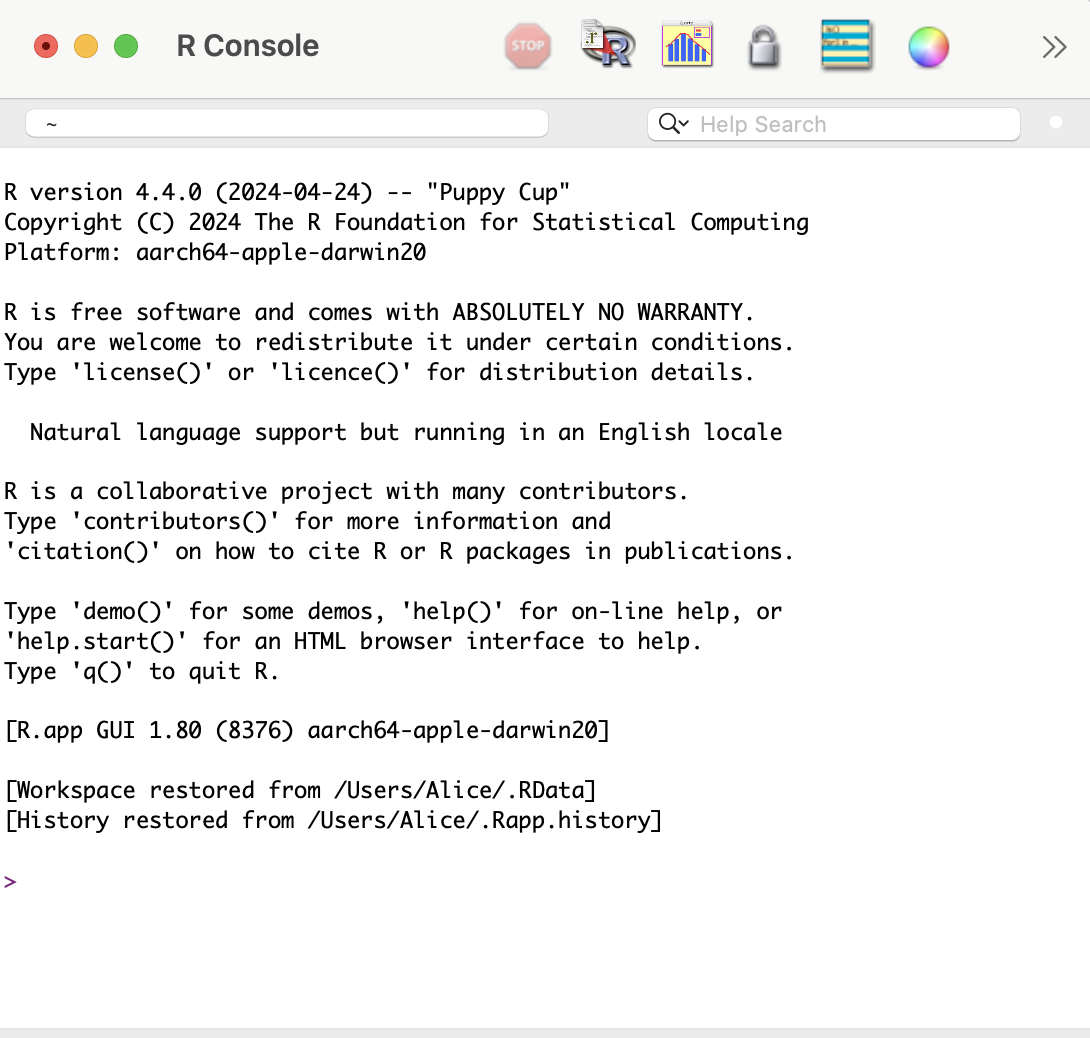
\includegraphics[width=0.75\textwidth,height=\textheight]{book/images/intro_to_r/r-console.png}

}

\caption{\label{fig-r-console}The R Console.}

\end{figure}%

To start, type \texttt{2+3} and press ENTER. You should see that
\texttt{5} is printed below that code and that your cursor is moved to
the next line.

\subsection{Basic Computations and
Objects}\label{basic-computations-and-objects}

In the previous example, we coded a simple addition. Try out some other
basic calculations using the following operators \index{R operators}:

\begin{itemize}
\tightlist
\item
  Addition: \texttt{5+6}\\
\item
  Subtraction: \texttt{7-2}\\
\item
  Multiplication: \texttt{2*3}\\
\item
  Division: \texttt{6/3}\\
\item
  Exponentiation: \texttt{4\^{}2}\\
\item
  Modulo: \texttt{100\ \%\%\ 4}
\end{itemize}

For example, use the modulo operator to find what 100 mod 4 is. It
should return 0 since 100 is divisible by 4.

If we want to save the result of any computation, we need to create an
object to store our value of interest. An \textbf{object}\index{objects}
is simply a named data structure that allows us to reference that data
structure. Objects are also commonly called
\textbf{variables}\index{variables}. In the following code, we create an
object \texttt{x} which stores the value \texttt{5} using the assignment
operator \texttt{\textless{}-}\index{R operators!assignment}. The
assignment operator assigns whatever is on the right-hand side of the
operator to the name on the left-hand side. We can now reference
\texttt{x} by calling its name. Additionally, we can update its value by
adding 1. In the second line of code, the computer first finds the value
of the right-hand side by finding the current value of \texttt{x} before
adding 1 and assigning it back to \texttt{x}.

\begin{Shaded}
\begin{Highlighting}[]
\NormalTok{x }\OtherTok{\textless{}{-}} \DecValTok{2}\SpecialCharTok{+}\DecValTok{3}
\NormalTok{x }\OtherTok{\textless{}{-}}\NormalTok{ x}\SpecialCharTok{+}\DecValTok{1}
\NormalTok{x}
\CommentTok{\#\textgreater{} [1] 6}
\end{Highlighting}
\end{Shaded}

We can create and store multiple objects by using different names. The
following code creates a new object \texttt{y} that is one more than the
value of \texttt{x}. We can see that the value of \texttt{x} is still
\texttt{5} after running this code.

\begin{Shaded}
\begin{Highlighting}[]
\NormalTok{x }\OtherTok{\textless{}{-}} \DecValTok{2}\SpecialCharTok{+}\DecValTok{3}
\NormalTok{y }\OtherTok{\textless{}{-}}\NormalTok{ x}
\NormalTok{y }\OtherTok{\textless{}{-}}\NormalTok{ y }\SpecialCharTok{+} \DecValTok{1}
\NormalTok{x}
\CommentTok{\#\textgreater{} [1] 5}
\end{Highlighting}
\end{Shaded}

\subsection{Naming Conventions}\label{naming-conventions}

As we start creating objects, we want to make sure we use good object
names\index{naming convention}. Here are a few tips for naming objects
effectively:

\begin{itemize}
\tightlist
\item
  Stick to a single format. We use \textbf{snake\_case}, which uses
  underscores between words (e.g., \texttt{my\_var},
  \texttt{class\_year}).\\
\item
  Make your names useful. Try to avoid using names that are too long\\
  (e.g., \texttt{which\_day\_of\_the\_week}) or that do not contain
  enough information (e.g., \texttt{x1}, \texttt{x2}, \texttt{x3}).\\
\item
  Replace unexplained numeric values with named objects. For example, if
  you need to do some calculations using 100 as the number of
  participants, create an object \texttt{n\_part} with value 100 rather
  than repeatedly using the number. This makes the code easy to update
  and helps the user avoid possible errors.
\end{itemize}

\section{RStudio and Quarto}\label{rstudio-and-quarto}

If we made a mistake in the code we typed in the console, we would have
to re-enter everything from the beginning. However, when we write code,
we often want to be able to run it multiple times and develop it in
stages. R Scripts \index{R Script} and R Markdown \index{R Markdown}
files allow us to save all of our R code in files that we can update and
re-run, which allows us to create reproducible and easy-to-share
analyses. We now move to RStudio \index{RStudio!development environment}
as our development environment to demonstrate creating an R Script. When
you open RStudio, there are multiple windows. Start by opening a new R
file by going to File -\textgreater{} New File -\textgreater{} R Script.
You should now see several windows as outlined in
Figure~\ref{fig-rstudio}.

\begin{figure}

\centering{

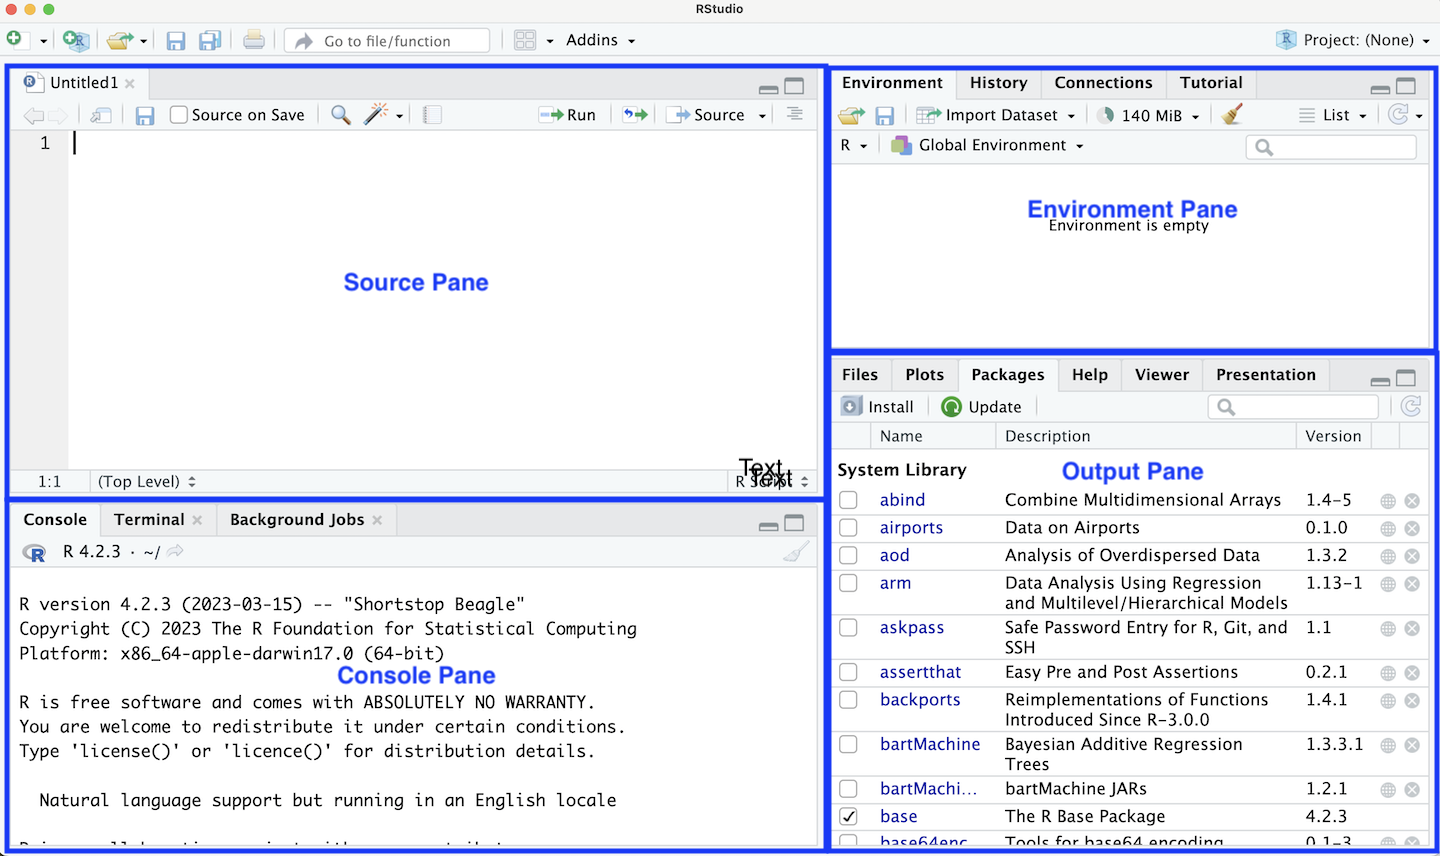
\includegraphics[width=4.86111in,height=\textheight]{book/images/intro_to_r/rstudio.png}

}

\caption{\label{fig-rstudio}RStudio Layout and Panes.}

\end{figure}%

\subsection{Panes}\label{panes}

There are four panes\index{RStudio!panes} shown by default:

\begin{itemize}
\item
  \textbf{Source Pane} - used for editing code files such as R Scripts
  or Quarto documents.
\item
  \textbf{Console Pane} - used to show the live R session.
\item
  \textbf{Environment Pane} - contains the Environment and History tabs,
  used to keep track of the current state.
\item
  \textbf{Output Pane} - contains the Plots and Packages tabs.
\end{itemize}

The source pane is the code editor window in the top left. This shows
your currently blank R Script. Add the following code to your .R file
and save the file as ``test.R''. Note that here we used snake\_case to
name our objects!

\begin{Shaded}
\begin{Highlighting}[]
\CommentTok{\# Calculate primary care physician to specialist ratio}
\NormalTok{pcp\_phys }\OtherTok{\textless{}{-}} \FunctionTok{c}\NormalTok{(}\DecValTok{6300}\NormalTok{, }\DecValTok{1080}\NormalTok{, }\DecValTok{9297}\NormalTok{, }\DecValTok{16433}\NormalTok{)}
\NormalTok{spec\_phys }\OtherTok{\textless{}{-}} \FunctionTok{c}\NormalTok{(}\DecValTok{6750}\NormalTok{, }\DecValTok{837}\NormalTok{, }\DecValTok{10517}\NormalTok{, }\DecValTok{22984}\NormalTok{)}
\NormalTok{pcp\_spec\_ratio }\OtherTok{\textless{}{-}} \DecValTok{1000} \SpecialCharTok{*}\NormalTok{ pcp\_phys }\SpecialCharTok{/}\NormalTok{ spec\_phys}
\end{Highlighting}
\end{Shaded}

The first line starts with \texttt{\#} and does not contain any code.
This is a \textbf{comment} line\index{comments}, which allows us to add
context, intent, or extra information to help the reader understand our
code. A good rule of thumb is that we want to write enough comments so
that we could open our code in 6 months and be able to understand what
we were doing. As we develop longer chunks of code, this will become
more important.

Unlike when we type code into the console, we can write multiple lines
of code in our R Script without running them. In order to run the code
in the script, we need to tell RStudio we are ready to run it. To run a
single line of code, we can either hit Ctrl+Enter when on that line or
we can hit the Run button
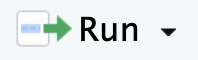
\includegraphics[width=0.55556in,height=\textheight]{book/images/intro_to_r/run-script.png}
at the top right of the source pane. This copies the code to the R
Console. Try this out to run the first line of code that defines
\texttt{pcp\_phys}. You can see that the line of code has been run in
the console pane. Now check your environment
pane\index{RStudio!object environment}. You should see that you have a
new object representing the one we just created. This pane keeps track
of all current objects. Run the second line of code and see how the
environment updates. If you look at the History tab within this pane,
you see the history of R commands run.

If we want to run all lines of code in our script, we can use the Source
button

\includegraphics[width=0.55556in,height=\textheight]{book/images/intro_to_r/source.png}.
Before we do this, we will clear our environment. You can do this by
clicking the broom

\includegraphics[width=0.27778in,height=\textheight]{book/images/intro_to_r/broom.png}
in the environment pane, which deletes all objects in the environment.
Alternatively, you can go to Session -\textgreater{} Restart R in the
main menu, which restarts your whole R session. After clearing your
environment, click the Source button. You will see that in the R Console
it shows that it sourced this file. This means that it runs through all
lines of code in this file. You can see that our objects have been added
back into our environment.

\begin{Shaded}
\begin{Highlighting}[]
\FunctionTok{source}\NormalTok{(}\StringTok{"test.R"}\NormalTok{)}
\end{Highlighting}
\end{Shaded}

Now suppose we want to update our script by adding a plot. Copy the code
in a subsequent code chunk, save your updated file, and then source your
file. You will see that the generated plot will appear in your output
pane.

\begin{Shaded}
\begin{Highlighting}[]
\FunctionTok{plot}\NormalTok{(spec\_phys, pcp\_phys)}
\end{Highlighting}
\end{Shaded}

\begin{center}
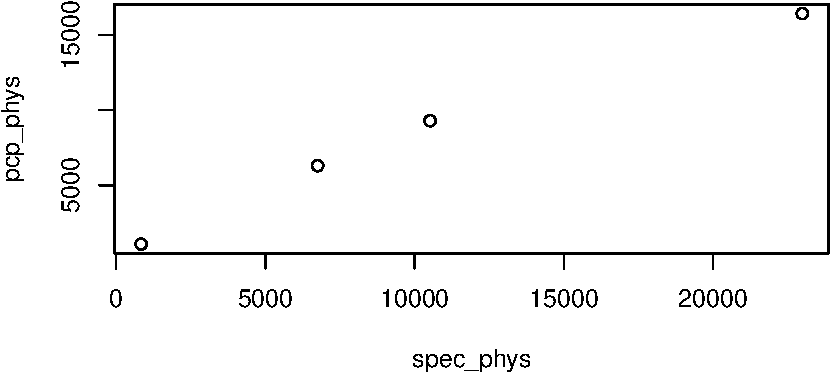
\includegraphics[width=1\textwidth,height=\textheight]{book/intro_to_r_files/figure-pdf/unnamed-chunk-5-1.pdf}
\end{center}

Unlike R Scripts which only contain R code, Quarto
\index{Quarto!documents} documents allow us to intersperse text and
code. This breaks our code into chunks surrounded by text written in
Markdown. Every chapter in this book is available as a Quarto document.
Try opening the Quarto file for Chapter~\ref{sec-data-structures} of
this book. You will see the first \textbf{code chunk}
\index{Quarto!code chunk} as in Figure~\ref{fig-code-chunk}. In order to
run the code in a code chunk, we can again use Ctrl+Enter to run a
single line or selected lines. Additionally, we can use the Play button

\includegraphics[width=0.27778in,height=\textheight]{book/images/intro_to_r/run-current-chunk.png}.
This runs all the code within the chunk. We recommend using the
available Quarto documents to follow along with the text. Writing your
own Quarto documents is covered in Chapter~\ref{sec-quarto}.

\begin{figure}

\centering{

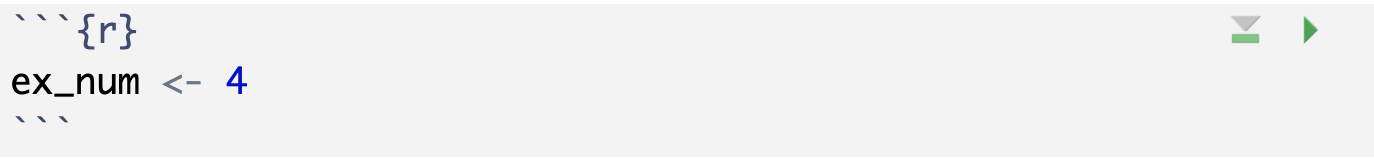
\includegraphics[width=4.16667in,height=\textheight]{book/images/intro_to_r/ex-code-chunk.png}

}

\caption{\label{fig-code-chunk}Example Code Chunk.}

\end{figure}%

\subsection{Calling Functions}\label{calling-functions}

When we use R, we have access to all the functions available in base R.
A \textbf{function}\index{functions} takes in one or more inputs and
returns a single output object. Let's first use the simple function
\texttt{exp()}\index{R functions!exp()@\texttt{exp()}}. This exponential
function takes in one (or more) numeric values and exponentiates them.
The following code computes \(e^3\).

\begin{Shaded}
\begin{Highlighting}[]
\FunctionTok{exp}\NormalTok{(}\DecValTok{3}\NormalTok{)}
\CommentTok{\#\textgreater{} [1] 20.1}
\end{Highlighting}
\end{Shaded}

Some other simple functions are shown that all convert a numeric input
to an integer value. The
\texttt{ceiling()}\index{R functions!ceiling()@\texttt{ceiling()}} and
\texttt{floor()}\index{R functions!floor()@\texttt{floor()}} functions
return the ceiling and floor of your input, and the
\texttt{round()}\index{R functions!round()@\texttt{round()}} function
rounds your input to the closest integer. Note that the \texttt{round()}
function rounds a number ending in 0.5 to the closest even integer.

\begin{Shaded}
\begin{Highlighting}[]
\FunctionTok{ceiling}\NormalTok{(}\FloatTok{3.7}\NormalTok{)}
\CommentTok{\#\textgreater{} [1] 4}
\end{Highlighting}
\end{Shaded}

\begin{Shaded}
\begin{Highlighting}[]
\FunctionTok{floor}\NormalTok{(}\FloatTok{3.7}\NormalTok{)}
\CommentTok{\#\textgreater{} [1] 3}
\end{Highlighting}
\end{Shaded}

\begin{Shaded}
\begin{Highlighting}[]
\FunctionTok{round}\NormalTok{(}\FloatTok{2.5}\NormalTok{)}
\CommentTok{\#\textgreater{} [1] 2}
\FunctionTok{round}\NormalTok{(}\FloatTok{3.5}\NormalTok{)}
\CommentTok{\#\textgreater{} [1] 4}
\end{Highlighting}
\end{Shaded}

If we want to learn about a function, we can use the help operator
\texttt{?} \index{help operator} by typing it in front of the function
we are interested in: this brings up the documentation
\index{functions!documentation} for that particular function. This
documentation often tells you the usage of the function, the
\textbf{arguments} \index{functions!arguments} (the object inputs) and
the \textbf{value} \index{functions!return value} (information about the
returned object), and it gives some examples of how to use the function.
For example, if we want to understand the difference between
\texttt{floor()} and \texttt{ceiling()}, we can call \texttt{?floor} and
\texttt{?ceiling}. This should bring up the documentation in your help
window. We can then read that the floor function rounds a numeric input
down to the nearest integer, whereas the ceiling function rounds a
numeric input up to the nearest integer.

\subsection{Working Directories and
Paths}\label{working-directories-and-paths}

Let's try using another example function:
\texttt{read.csv()}\index{R functions!read.csv()@\texttt{read.csv()}}.
This function reads in a comma-delimited file and returns the
information as a data frame (try typing \texttt{?read.csv} in the
console to read more about this function). We learn more about data
frames in Chapter~\ref{sec-data-structures}. The first argument to this
function is a file, which can be expressed as either a file name or a
path to a file. First, download the file \texttt{fake\_names.csv} from
this book's
\href{https://github.com/alicepaul/health-data-science-using-r/tree/main/book/data}{github
repository}. By default, R looks for the file in your current working
directory\index{working directory} To find the working directory, you
can run \texttt{getwd()}\index{R functions!getwd()@\texttt{getwd()}}.
You can see in the following output that my current working directory is
where the book content is on my computer.

\begin{Shaded}
\begin{Highlighting}[]
\FunctionTok{getwd}\NormalTok{()}
\CommentTok{\#\textgreater{} [1] "/Users/Alice/Dropbox/health{-}data{-}science{-}using{-}r/book"}
\end{Highlighting}
\end{Shaded}

You can either move the .csv file to your current working directory and
load it in, or you can specify the path to the .csv file. Another option
is to update your working directory by using the
\texttt{setwd()}\index{R functions!setwd()@\texttt{setwd()}} function.

\begin{Shaded}
\begin{Highlighting}[]
\FunctionTok{setwd}\NormalTok{(}\StringTok{\textquotesingle{}/Users/Alice/Dropbox/health{-}data{-}science{-}using{-}r/book/data\textquotesingle{}}\NormalTok{)}
\end{Highlighting}
\end{Shaded}

If you receive an error that a file cannot be found, you most likely
have the wrong path to the file or the wrong file name. In the following
code, I chose to specify the path to the downloaded .csv file, saved
this file to an object called \texttt{df}, and then printed that
\texttt{df} object.

\begin{Shaded}
\begin{Highlighting}[]
\CommentTok{\# update this with the path to your file}
\NormalTok{df }\OtherTok{\textless{}{-}} \FunctionTok{read.csv}\NormalTok{(}\StringTok{"data/fake\_names.csv"}\NormalTok{) }
\NormalTok{df}
\CommentTok{\#\textgreater{}                  Name Age     DOB            City State}
\CommentTok{\#\textgreater{} 1           Ken Irwin  37 6/28/85      Providence    RI}
\CommentTok{\#\textgreater{} 2 Delores Whittington  56 4/28/67      Smithfield    RI}
\CommentTok{\#\textgreater{} 3       Daniel Hughes  41 5/22/82      Providence    RI}
\CommentTok{\#\textgreater{} 4         Carlos Fain  83  2/2/40          Warren    RI}
\CommentTok{\#\textgreater{} 5        James Alford  67 2/23/56 East Providence    RI}
\CommentTok{\#\textgreater{} 6        Ruth Alvarez  34 9/22/88      Providence    RI}
\end{Highlighting}
\end{Shaded}

We can see that \texttt{df} contains the information from the .csv file,
and that R has printed the first few observations of the data.

\subsection{Installing and Loading
Packages}\label{installing-and-loading-packages}

When working with data frames, we often use the \textbf{tidyverse}
package (Wickham 2023)\index{R packages!tidyverse}, which is actually a
collection of R packages for data science applications. An R package
\index{R packages} is a collection of functions and/or sample data that
allow us to expand on the functionality of R beyond the base functions.
You can check whether you have the \textbf{tidyverse} package installed
by going to the Package tab in the Output Pane in RStudio or by running
the following command, which displays all your installed packages.

\texttt{installed.packages()}

If you don't already have a package installed, you can install it using
the \texttt{install.packages()}
function\index{R packages!installing}\index{R functions!install.packages()@\texttt{install.packages()}}.
Note that you have to include single or double quotes around the package
name when using this function. You only have to install a package one
time.

\texttt{install.packages(\textquotesingle{}tidyverse\textquotesingle{})}

The function
\texttt{read\_csv()}\index{R functions!read\textunderscore csv()@\texttt{read\textunderscore csv()}}
is another function to read in comma-delimited files that is part of the
\textbf{readr} package\index{R packages!readr} in the \textbf{tidyverse}
(Wickham, Hester, and Bryan 2023). However, if we tried to use this
function to load in our data, we would get an error that the function
cannot be found. That is because we haven't loaded in this package. To
do so, we use the
\texttt{library()}\index{R functions!library()@\texttt{library()}}
function. Unlike the \texttt{install.packages()} function, we do not
have to use quotes around the package name when calling this
\texttt{library()} function. When we load in a package, we see some
messages. For example, in the following output we see that this package
contains the functions \texttt{filter()} and \texttt{lag()} that are
also functions in base R. In future chapters, we suppress these messages
to make the chapter presentation nicer. After loading the
\textbf{tidyverse} package, we can now use the \texttt{read\_csv()}
function.

\begin{Shaded}
\begin{Highlighting}[]
\FunctionTok{library}\NormalTok{(tidyverse)}
\end{Highlighting}
\end{Shaded}

\begin{Shaded}
\begin{Highlighting}[]
\NormalTok{df }\OtherTok{\textless{}{-}} \FunctionTok{read\_csv}\NormalTok{(}\StringTok{"data/fake\_names.csv"}\NormalTok{, }\AttributeTok{show\_col\_types=}\ConstantTok{FALSE}\NormalTok{)}
\NormalTok{df}
\CommentTok{\#\textgreater{} \# A tibble: 6 x 5}
\CommentTok{\#\textgreater{}   Name                  Age DOB     City            State}
\CommentTok{\#\textgreater{}   \textless{}chr\textgreater{}               \textless{}dbl\textgreater{} \textless{}chr\textgreater{}   \textless{}chr\textgreater{}           \textless{}chr\textgreater{}}
\CommentTok{\#\textgreater{} 1 Ken Irwin              37 6/28/85 Providence      RI   }
\CommentTok{\#\textgreater{} 2 Delores Whittington    56 4/28/67 Smithfield      RI   }
\CommentTok{\#\textgreater{} 3 Daniel Hughes          41 5/22/82 Providence      RI   }
\CommentTok{\#\textgreater{} 4 Carlos Fain            83 2/2/40  Warren          RI   }
\CommentTok{\#\textgreater{} 5 James Alford           67 2/23/56 East Providence RI   }
\CommentTok{\#\textgreater{} 6 Ruth Alvarez           34 9/22/88 Providence      RI}
\end{Highlighting}
\end{Shaded}

Alternatively, we could have told R where to locate the function by
adding \texttt{readr::} before the function. This tells it to find
\texttt{read\_csv()} function in the \textbf{readr} package. This can be
helpful even if we have already loaded in the package, since sometimes
multiple packages have functions with the same name.

\begin{Shaded}
\begin{Highlighting}[]
\NormalTok{df }\OtherTok{\textless{}{-}}\NormalTok{ readr}\SpecialCharTok{::}\FunctionTok{read\_csv}\NormalTok{(}\StringTok{"data/fake\_names.csv"}\NormalTok{, }\AttributeTok{show\_col\_types =} \ConstantTok{FALSE}\NormalTok{)}
\end{Highlighting}
\end{Shaded}

\section{RStudio Projects and RStudio Global
Options}\label{rstudio-projects-and-rstudio-global-options}

You have now had a basic tour of RStudio. Once you close RStudio, you
have the option of whether to store your current R environment. We
highly recommend that you update your RStudio options
\index{RStudio!global options} to not save your workspace on exiting or
load it on starting. This ensures that you have a fresh environment
every time you open RStudio and helps you to create fully reproducible
code and avoid possible errors or confusion
(Figure~\ref{fig-global-options}).

\begin{figure}

\centering{

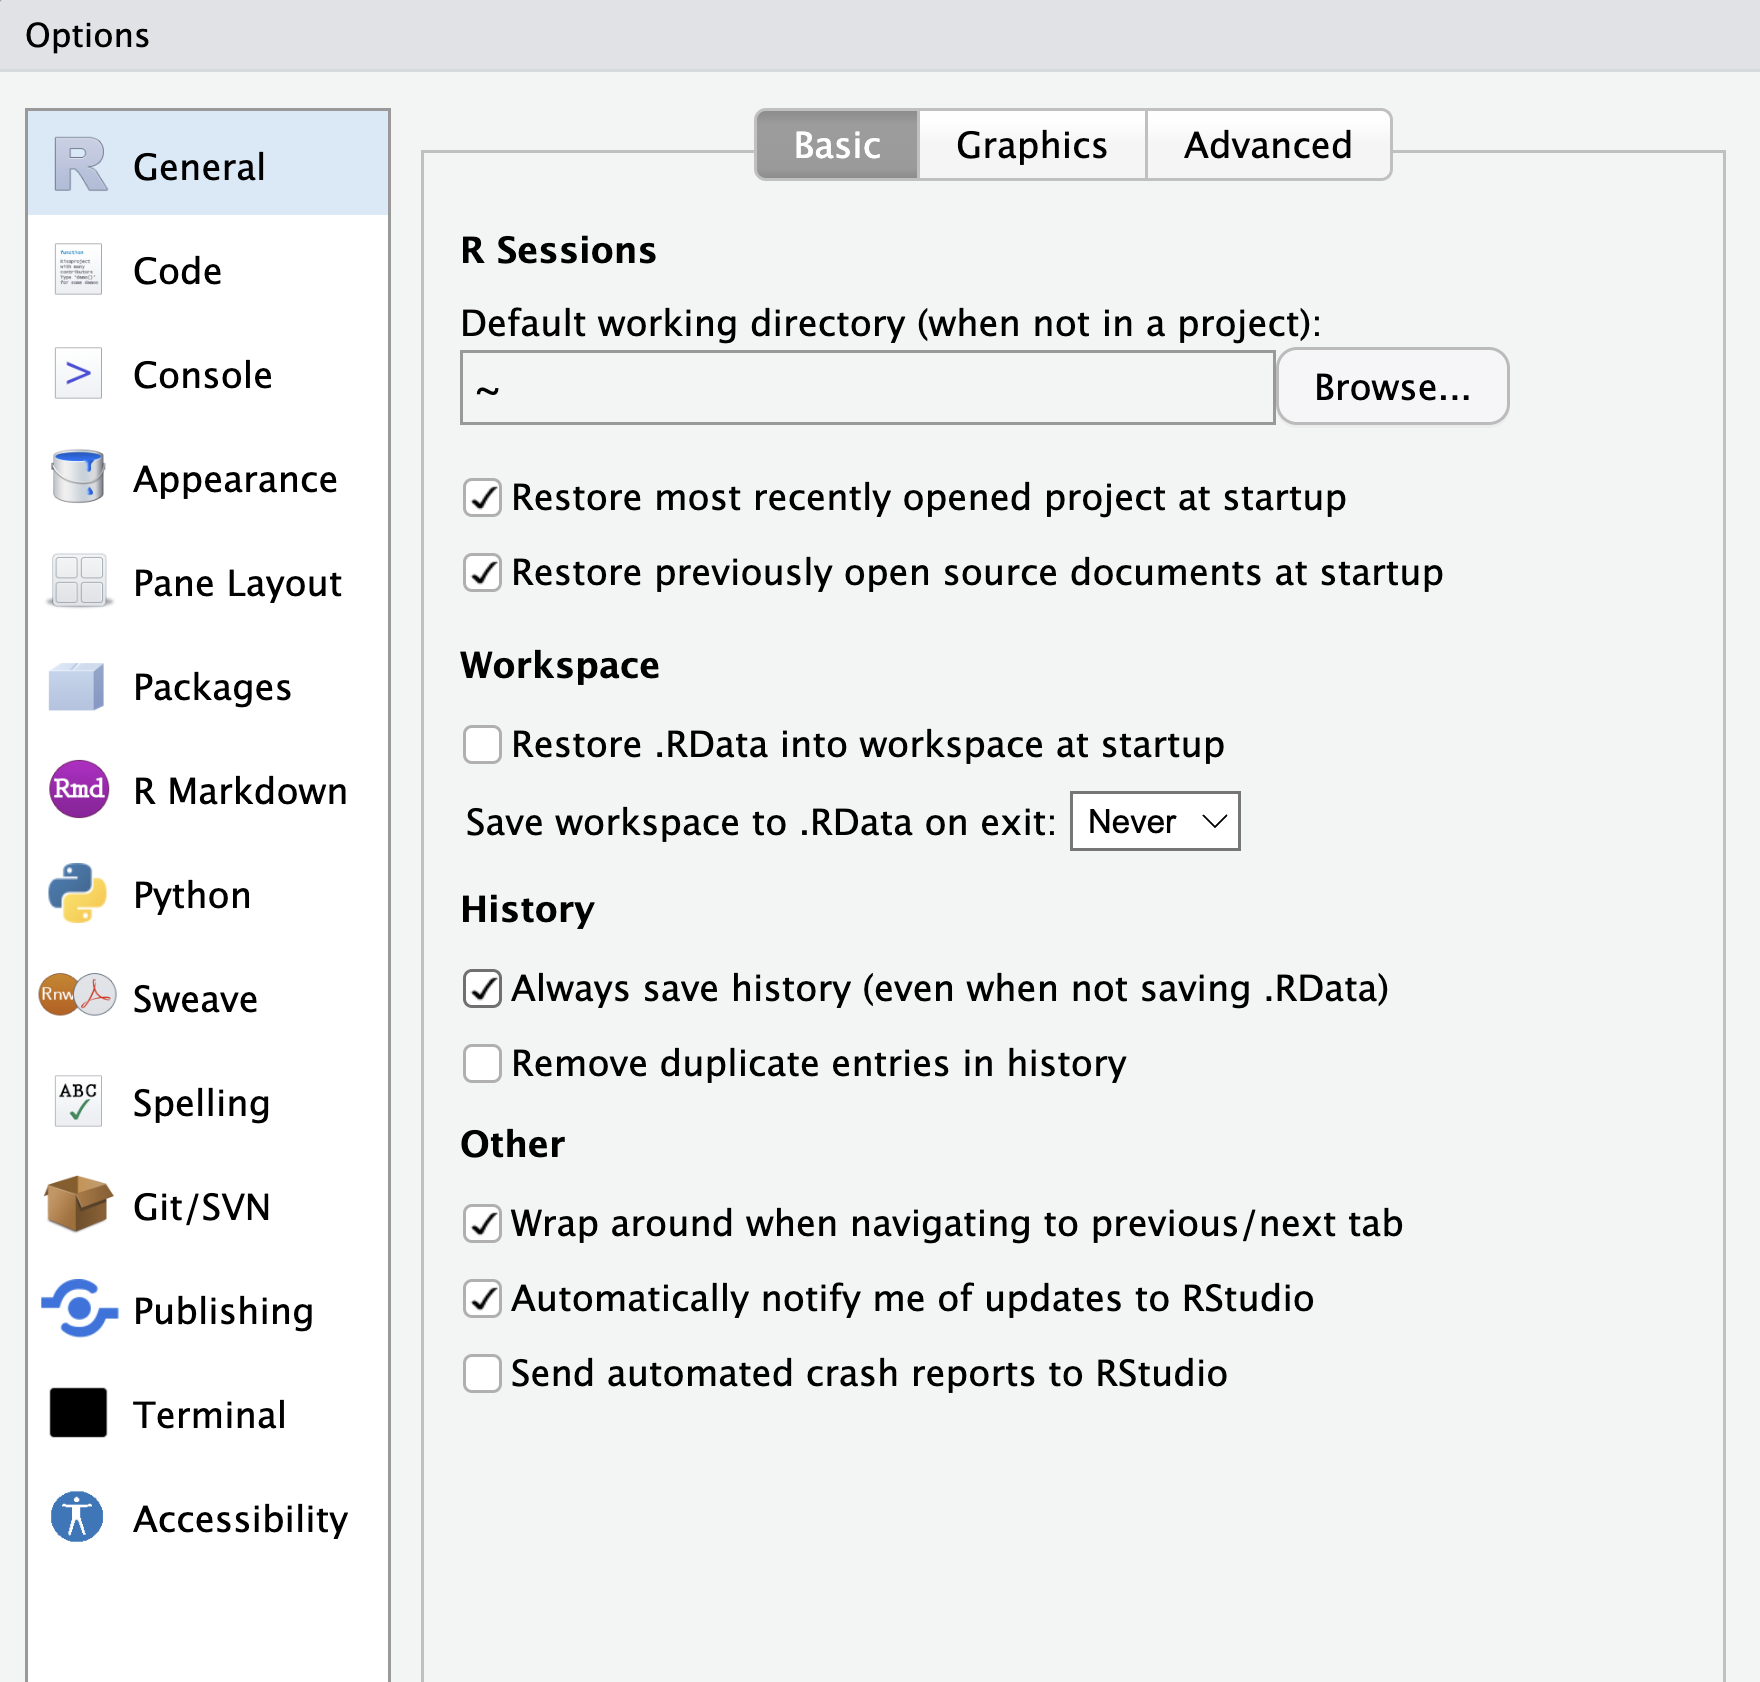
\includegraphics[width=0.7\textwidth,height=\textheight]{book/images/intro_to_r/rstudio-global-opts.png}

}

\caption{\label{fig-global-options}RStudio Global Options.}

\end{figure}%

Now when you re-open RStudio, it opens the files you had open previously
and has your history of commands. This may become confusing when you are
working on different files. RStudio projects allow us to create a folder
that is associated with a single project. This means that when we open
our project, it sets the appropriate work directory for us and only
opens files related to that project. In order to create a new R
project\index{RStudio!projects}, such as one associated with this book,
you can go to File -\textgreater{} New Project. You can then choose
whether to create a new directory or existing directory before selecting
to create an empty project as in Figure~\ref{fig-new-project}. Within
this directory you should see a .RProj file that allows you to re-open
your project.

\begin{figure}

\centering{

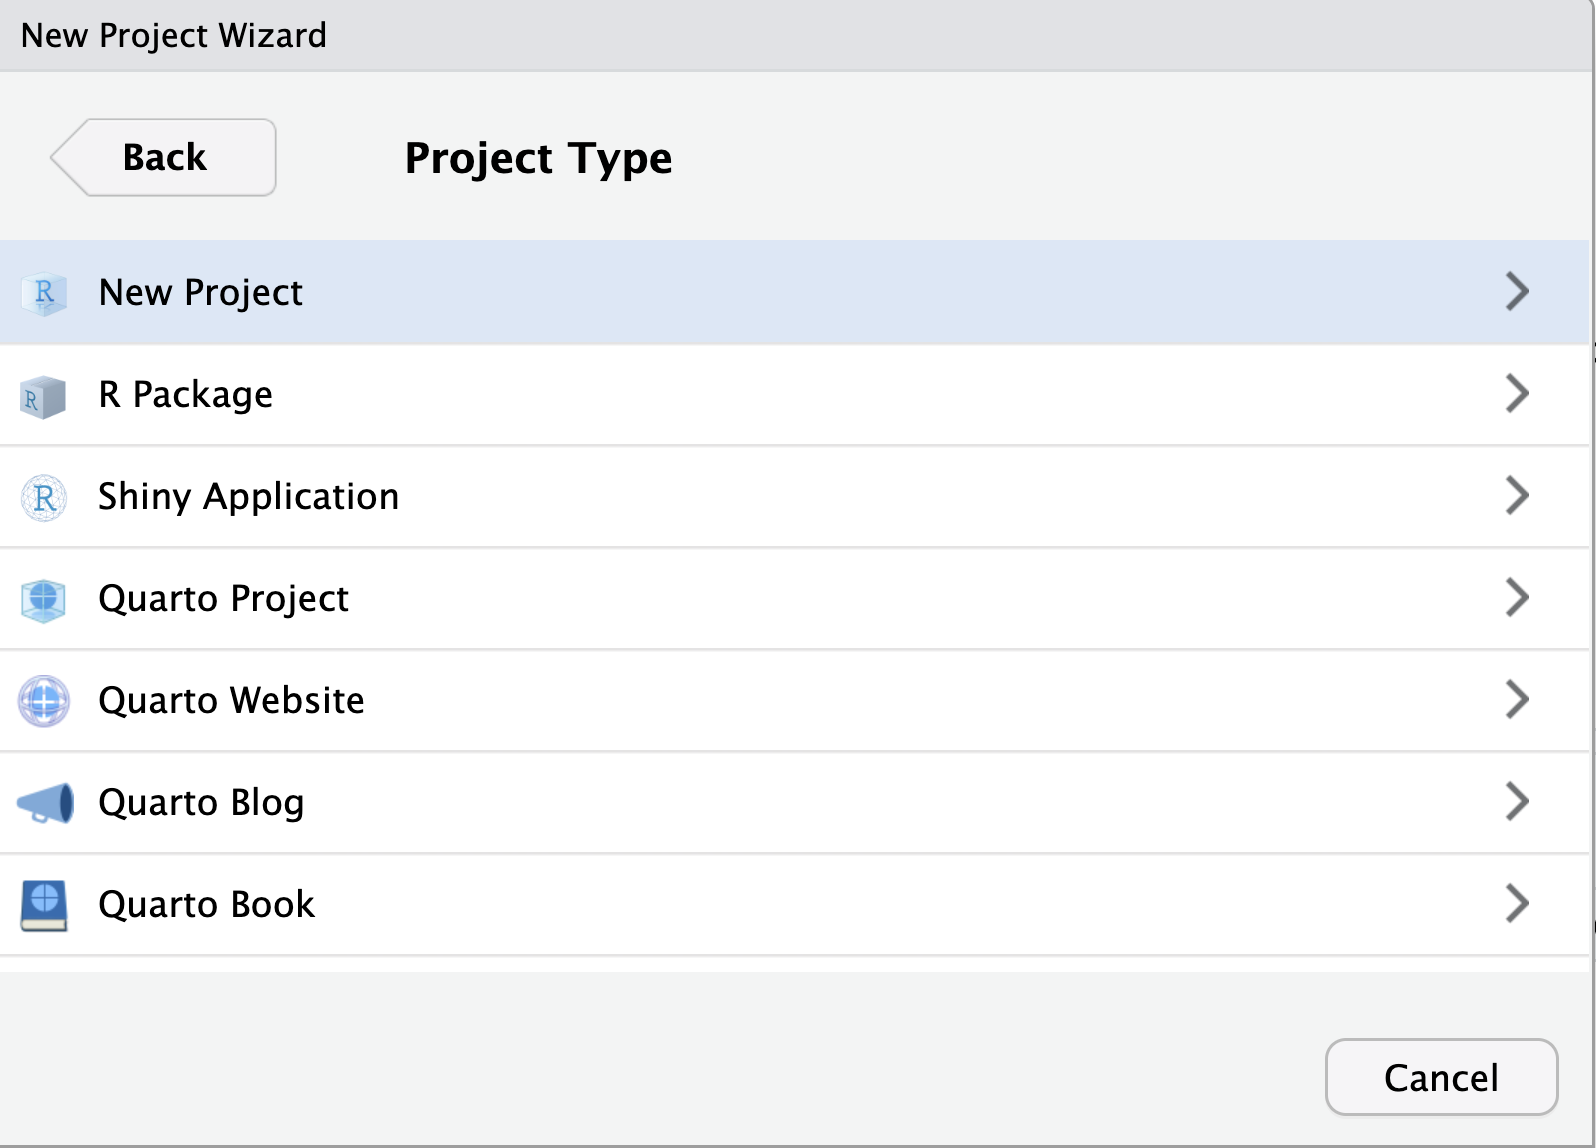
\includegraphics[width=0.7\textwidth,height=\textheight]{book/images/intro_to_r/new-project.png}

}

\caption{\label{fig-new-project}Creating a New RStudio Project.}

\end{figure}%

\section{Tips and Reminders}\label{tips-and-reminders}

We end this chapter with some final tips and reminders.

\begin{itemize}
\item
  \textbf{Keyboard shortcuts}: RStudio has several useful keyboard
  shortcuts that make your programming experience more streamlined. It
  is worth getting familiar with some of the most common keyboard
  shortcuts using this book's
  \href{https://github.com/alicepaul/health-data-science-using-r/blob/main/book/refs/r_studio_keyboard_shortcuts.pdf}{cheat
  sheet}.
\item
  \textbf{Asking for help}: Within R, you can use the \texttt{?}
  operator or the \texttt{help()}
  \index{R functions!help()@\texttt{help()}} function to pull up
  documentation on a given function. This documentation is also
  available \href{https://rdocumentation.org/}{online}.
\item
  \textbf{Finding all objects}: You can use the environment pane or
  \texttt{ls()} \index{R functions!ls()@\texttt{ls()}} function to find
  all current objects. If you have an error that an object you are
  calling does not exist, take a look to find where you defined it.
\item
  \textbf{Checking packages}: If you get an error that a function does
  not exist, check to make sure you have loaded that package using the
  \texttt{library()} function. The list of packages used in this book is
  given on the GitHub repository homepage.
\end{itemize}

\chapter{Data Structures in R}\label{sec-data-structures}

In this chapter, we demonstrate the key \textbf{data
structures}\index{data structures} in R. Data structures are how
information is stored in R and refer to the types of objects we can
create in R. The data structures that we use inform R how to interpret
our code. Any \textbf{object}\index{object} is a named instance of a
data structure. For example, the object \texttt{ex\_num} is a vector of
numeric type.

\begin{Shaded}
\begin{Highlighting}[]
\NormalTok{ex\_num }\OtherTok{\textless{}{-}} \DecValTok{4}
\end{Highlighting}
\end{Shaded}

The main data structures in R are \textbf{vectors}, \textbf{factors},
\textbf{matrices}, \textbf{arrays}, \textbf{lists}, and \textbf{data
frames}. These structures are distinguished by their dimensions and by
the type of data they store. For example, we might have a
one-dimensional vector that contains all numeric values, or we could
have a two-dimensional data frame with rows and columns where we might
have one numeric column and one character column. In
Figure~\ref{fig-data-structures}, there are two vectors with different
types (character and numeric) on top, followed by a matrix and data
frame below. In this chapter, we cover each data structure except for
arrays. Arrays are an extension of matrices that allow for data that is
more than two-dimensional and are not needed for the applications
covered in this book.

\begin{figure}

\centering{

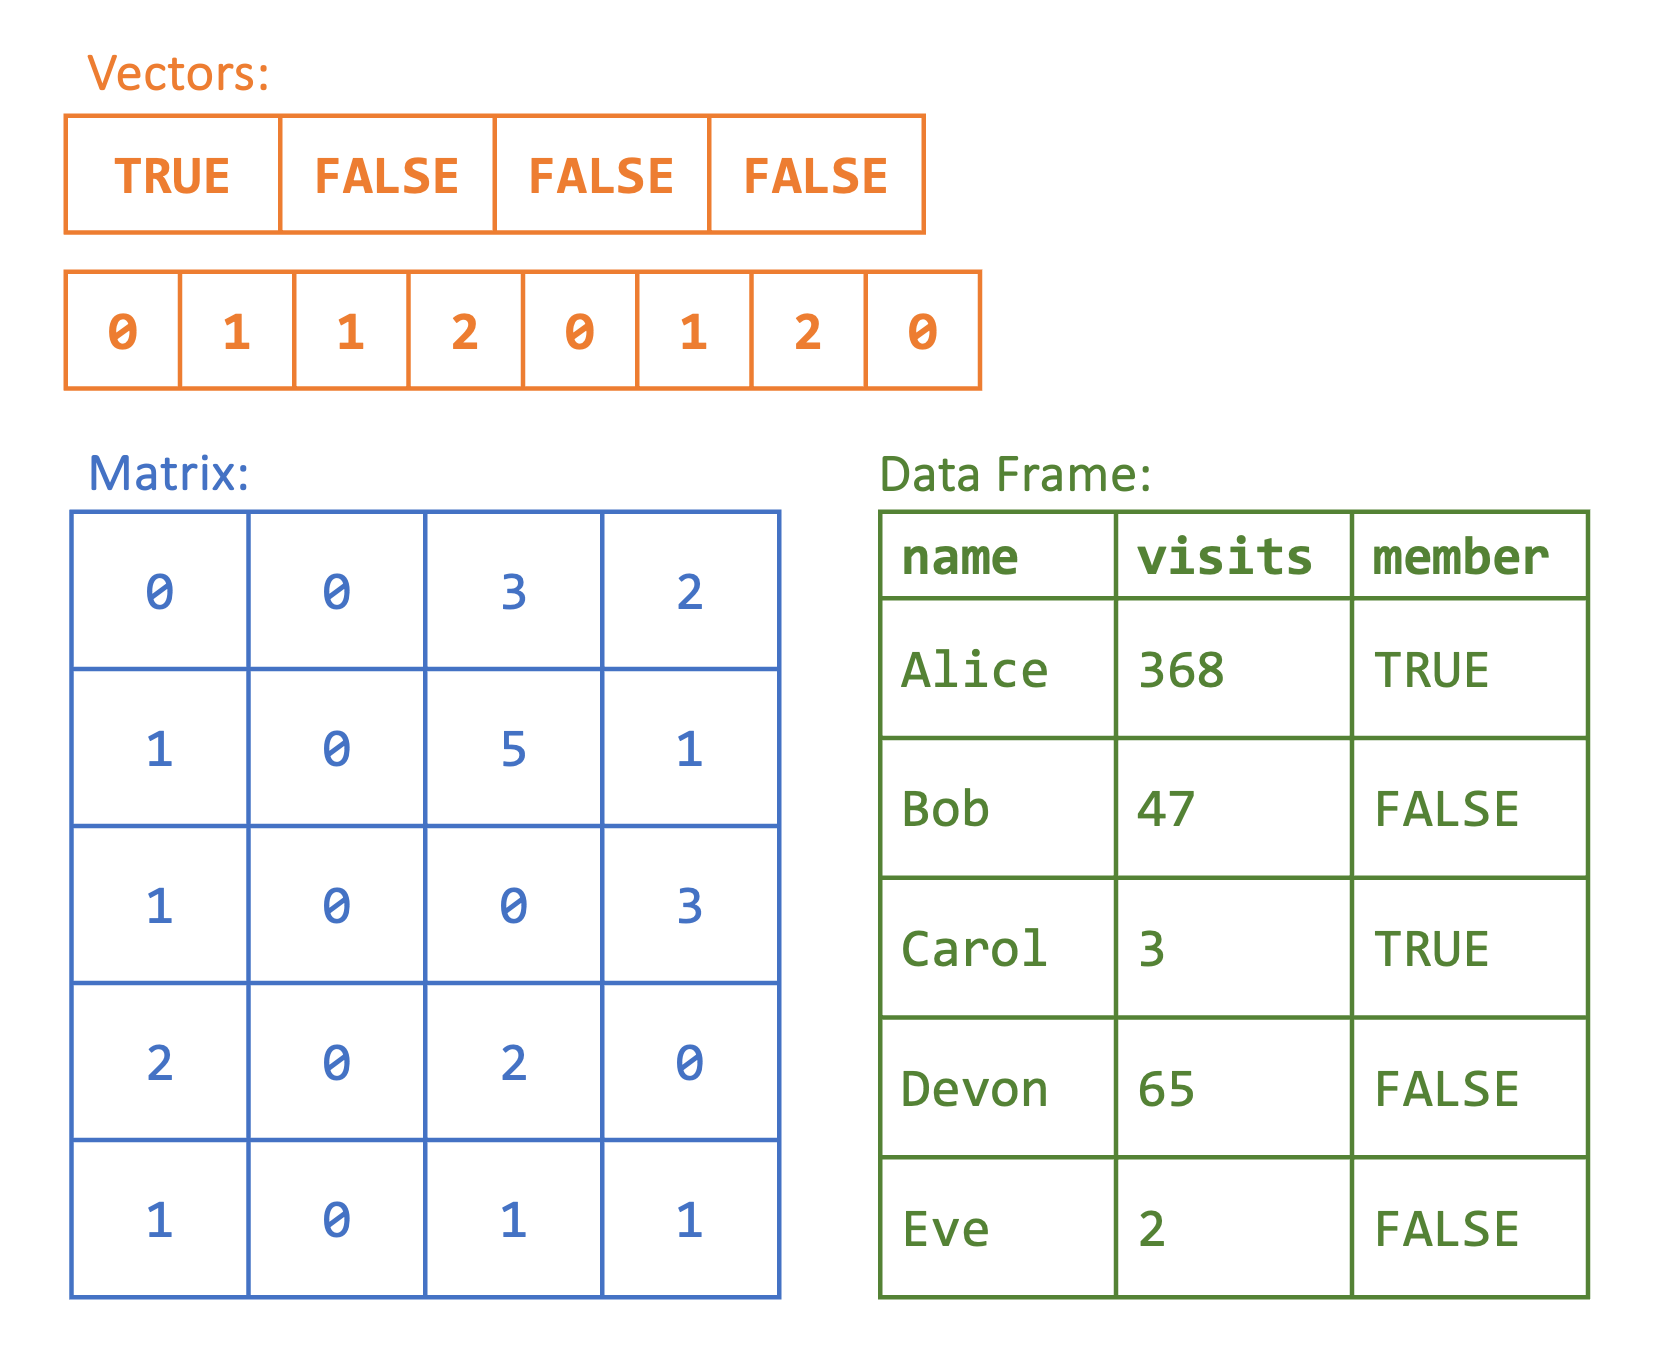
\includegraphics[width=0.8\textwidth,height=\textheight]{book/images/data_structures/data-structures.png}

}

\caption{\label{fig-data-structures}Data Structures.}

\end{figure}%

\section{\texorpdfstring{Data Types
\index{data types}}{Data Types }}\label{data-types}

Each individual value in R has a type: \textbf{logical},
\textbf{integer}, \textbf{double}, or \textbf{character}. We can think
of these as the building blocks of all data structures. We use the
\texttt{typeof()}\index{R functions!typeof()@\texttt{typeof()}} function
to find the type of our vector \texttt{ex\_num}, which shows that the
value of \texttt{ex\_num} is a \textbf{double}\index{data types!double}.
A double is a numeric value with a stored decimal.

\begin{Shaded}
\begin{Highlighting}[]
\FunctionTok{typeof}\NormalTok{(ex\_num)}
\CommentTok{\#\textgreater{} [1] "double"}
\end{Highlighting}
\end{Shaded}

On the other hand, an \textbf{integer}\index{data types!integer} is a
whole number that does not contain a decimal. We now create an integer
object \texttt{ex\_int}. To indicate to R that we want to restrict our
values to integer values, we use an \texttt{L} after the number.

\begin{Shaded}
\begin{Highlighting}[]
\NormalTok{ex\_int }\OtherTok{\textless{}{-}} \DecValTok{4}\NormalTok{L}
\FunctionTok{typeof}\NormalTok{(ex\_int)}
\CommentTok{\#\textgreater{} [1] "integer"}
\end{Highlighting}
\end{Shaded}

Both \texttt{ex\_num} and \texttt{ex\_int} are numeric objects, but we
can also work with two other types of objects:
\textbf{characters}\index{data types!character} (e.g., ``php'',
``stats'') and \textbf{Booleans}\index{data types!Boolean} (e.g., TRUE,
FALSE), also known as \textbf{logicals}\index{data types!logical}.

\begin{Shaded}
\begin{Highlighting}[]
\NormalTok{ex\_bool }\OtherTok{\textless{}{-}} \ConstantTok{TRUE}
\NormalTok{ex\_char }\OtherTok{\textless{}{-}} \StringTok{"Alice"}

\FunctionTok{typeof}\NormalTok{(ex\_bool)}
\CommentTok{\#\textgreater{} [1] "logical"}
\FunctionTok{typeof}\NormalTok{(ex\_char)}
\CommentTok{\#\textgreater{} [1] "character"}
\end{Highlighting}
\end{Shaded}

One important characteristic of logical objects is that R also
interprets them as 0/1. This means they can be added as in the following
example: each \texttt{TRUE} has a value of 1, and each \texttt{FALSE}
has a value of 0.

\begin{Shaded}
\begin{Highlighting}[]
\ConstantTok{TRUE} \SpecialCharTok{+} \ConstantTok{FALSE} \SpecialCharTok{+} \ConstantTok{TRUE}
\CommentTok{\#\textgreater{} [1] 2}
\end{Highlighting}
\end{Shaded}

To create all of these objects, we used the assignment
operator\index{assignment operator} \texttt{\textless{}-}, which we
discussed in Chapter~\ref{sec-intro-to-r}. You may see code elsewhere
that uses an \texttt{=} instead. While \texttt{=} can also be used for
assignment, it is more standard practice to use \texttt{\textless{}-}.

\section{\texorpdfstring{Vectors
\index{vectors}}{Vectors }}\label{vectors}

In the previous examples, we created objects with a single value. R
actually uses a vector of length 1 to store this information.
\textbf{Vectors} are one-dimensional data structures that can store
multiple data values of the same type (e.g., character, Boolean, or
numeric). See Figure~\ref{fig-vectors}.

\begin{figure}

\centering{

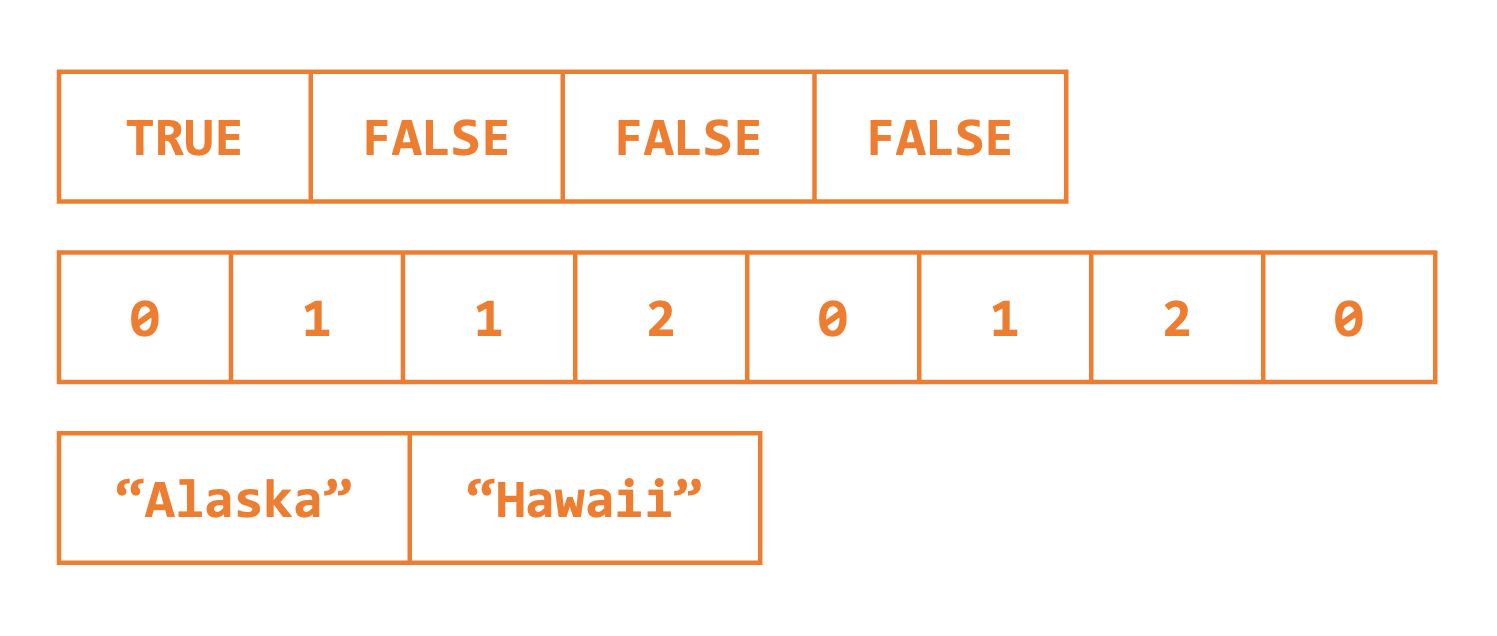
\includegraphics[width=0.6\textwidth,height=\textheight]{book/images/data_structures/vectors.png}

}

\caption{\label{fig-vectors}Vector Examples.}

\end{figure}%

We can confirm this by using the
\texttt{is.vector()}\index{R functions!is.vector()@\texttt{is.vector()}}
function, which returns whether or not the inputted argument is a
vector.

\begin{Shaded}
\begin{Highlighting}[]
\FunctionTok{is.vector}\NormalTok{(ex\_bool)}
\CommentTok{\#\textgreater{} [1] TRUE}
\end{Highlighting}
\end{Shaded}

One way to create a vector\index{vectors!create} with multiple values is
to use the combine function
\texttt{c()}\index{R functions!c()@\texttt{c()}}. In the following code,
we create two vectors: one with the days of the week and one with the
amount of rain on each day. The first vector has all character values,
and the second one has all numeric values.

\begin{Shaded}
\begin{Highlighting}[]
\NormalTok{days }\OtherTok{\textless{}{-}} \FunctionTok{c}\NormalTok{(}\StringTok{"Monday"}\NormalTok{, }\StringTok{"Tuesday"}\NormalTok{, }\StringTok{"Wednesday"}\NormalTok{, }\StringTok{"Thursday"}\NormalTok{, }\StringTok{"Friday"}\NormalTok{)}
\NormalTok{rain }\OtherTok{\textless{}{-}} \FunctionTok{c}\NormalTok{(}\DecValTok{5}\NormalTok{, }\FloatTok{0.1}\NormalTok{, }\DecValTok{0}\NormalTok{, }\DecValTok{0}\NormalTok{, }\FloatTok{0.4}\NormalTok{)}
\end{Highlighting}
\end{Shaded}

Remember, a vector can only store values of the same type. Because of
this, in the following code, R automatically converts the numeric value
to be a character in order to store these values in a vector together.

\begin{Shaded}
\begin{Highlighting}[]
\FunctionTok{c}\NormalTok{(}\StringTok{"Monday"}\NormalTok{, }\DecValTok{5}\NormalTok{)}
\CommentTok{\#\textgreater{} [1] "Monday" "5"}
\end{Highlighting}
\end{Shaded}

The \texttt{class()}\index{R functions!class()@\texttt{class()}}
function returns the data structure of an object. If we check the
classes of these two objects using the \texttt{class()} function, we see
that R tells us that the first is a character vector, and the second is
a numeric vector. This matches the data type in this case.

\begin{Shaded}
\begin{Highlighting}[]
\FunctionTok{class}\NormalTok{(days)}
\CommentTok{\#\textgreater{} [1] "character"}
\FunctionTok{class}\NormalTok{(rain)}
\CommentTok{\#\textgreater{} [1] "numeric"}
\end{Highlighting}
\end{Shaded}

What happens when we create an empty vector? What is the class?

\begin{Shaded}
\begin{Highlighting}[]
\NormalTok{ex\_empty }\OtherTok{\textless{}{-}} \FunctionTok{c}\NormalTok{()}
\FunctionTok{class}\NormalTok{(ex\_empty)}
\CommentTok{\#\textgreater{} [1] "NULL"}
\end{Highlighting}
\end{Shaded}

In this case, there is no specified type yet. If we wanted to specify
the type, we could make an empty vector using the
\texttt{vector()}\index{R functions!vector()@\texttt{vector()}}
function.

\begin{Shaded}
\begin{Highlighting}[]
\NormalTok{ex\_empty }\OtherTok{\textless{}{-}} \FunctionTok{vector}\NormalTok{(}\AttributeTok{mode =} \StringTok{"numeric"}\NormalTok{)}
\FunctionTok{class}\NormalTok{(ex\_empty)}
\CommentTok{\#\textgreater{} [1] "numeric"}
\end{Highlighting}
\end{Shaded}

Another way to create a vector is with the
\texttt{rep()}\index{R functions!rep()@\texttt{rep()}} or
\texttt{seq()}\index{R functions!seq()@\texttt{seq()}} functions. The
first function \texttt{rep(x,\ times)} takes in a vector \texttt{x} and
a number of \texttt{times} and outputs \texttt{x} repeated that many
times. Let's try this with a single value. The second function
\texttt{seq(from,\ to,\ step)} takes in a numeric starting value
\texttt{from}, end value \texttt{to}, and step size \texttt{step} and
returns a sequence starting at \texttt{from} in increments of
\texttt{step} until a maximum value of \texttt{to} is reached.

\begin{Shaded}
\begin{Highlighting}[]
\FunctionTok{rep}\NormalTok{(}\DecValTok{0}\NormalTok{, }\DecValTok{5}\NormalTok{)}
\CommentTok{\#\textgreater{} [1] 0 0 0 0 0}
\FunctionTok{rep}\NormalTok{(}\StringTok{"Monday"}\NormalTok{, }\DecValTok{4}\NormalTok{)}
\CommentTok{\#\textgreater{} [1] "Monday" "Monday" "Monday" "Monday"}
\FunctionTok{seq}\NormalTok{(}\DecValTok{1}\NormalTok{, }\DecValTok{5}\NormalTok{, }\DecValTok{1}\NormalTok{)}
\CommentTok{\#\textgreater{} [1] 1 2 3 4 5}
\FunctionTok{seq}\NormalTok{(}\DecValTok{0}\NormalTok{, }\SpecialCharTok{{-}}\DecValTok{10}\NormalTok{, }\SpecialCharTok{{-}}\DecValTok{2}\NormalTok{)}
\CommentTok{\#\textgreater{} [1]   0  {-}2  {-}4  {-}6  {-}8 {-}10}
\end{Highlighting}
\end{Shaded}

\subsection{\texorpdfstring{Indexing a Vector
\index{vectors!indexing}}{Indexing a Vector }}\label{indexing-a-vector}

Once we have a vector, we may want to access certain values stored in
that vector. To do so, we index the vector using the position of each
value: the first value in the vector has index 1, the second value has
index 2, etc. When we say a vector is one-dimensional, we mean that we
can define the position of each value by a single index. To index the
vector, we then use square brackets \texttt{{[}{]}} after the vector
name and provide the position. We use these indices to find the value at
index 1 and the value at index 4.

\begin{Shaded}
\begin{Highlighting}[]
\NormalTok{days[}\DecValTok{1}\NormalTok{]}
\CommentTok{\#\textgreater{} [1] "Monday"}
\NormalTok{days[}\DecValTok{4}\NormalTok{]}
\CommentTok{\#\textgreater{} [1] "Thursday"}
\end{Highlighting}
\end{Shaded}

We can either access a single value or a subset of values using a vector
of indices. Let's see what happens when we use a vector of indices
\texttt{c(1,4)} and then try using \texttt{-c(1,4)} and see what
happens. In the first case, we get the values at index 1 \emph{and} at
index 4. In the second case, we get all values \emph{except} at those
indices. The \texttt{-} indicates that we want to remove rather than
select these indices.

\begin{Shaded}
\begin{Highlighting}[]
\NormalTok{days[}\FunctionTok{c}\NormalTok{(}\DecValTok{1}\NormalTok{, }\DecValTok{4}\NormalTok{)]}
\CommentTok{\#\textgreater{} [1] "Monday"   "Thursday"}
\NormalTok{days[}\SpecialCharTok{{-}}\FunctionTok{c}\NormalTok{(}\DecValTok{1}\NormalTok{, }\DecValTok{4}\NormalTok{)]}
\CommentTok{\#\textgreater{} [1] "Tuesday"   "Wednesday" "Friday"}
\end{Highlighting}
\end{Shaded}

However, always indexing by the index value can sometimes be difficult
or inefficient. One extra feature of vectors is that we can associate a
name with each value\index{vectors!names}. In the subsequent code, we
update the names of the vector \texttt{rain} to be the days of the week
and then find Friday's rain count by indexing with the name.

\begin{Shaded}
\begin{Highlighting}[]
\FunctionTok{names}\NormalTok{(rain) }\OtherTok{\textless{}{-}}\NormalTok{ days}
\FunctionTok{print}\NormalTok{(rain)}
\CommentTok{\#\textgreater{}    Monday   Tuesday Wednesday  Thursday    Friday }
\CommentTok{\#\textgreater{}       5.0       0.1       0.0       0.0       0.4}
\NormalTok{rain[}\StringTok{"Friday"}\NormalTok{]}
\CommentTok{\#\textgreater{} Friday }
\CommentTok{\#\textgreater{}    0.4}
\end{Highlighting}
\end{Shaded}

The last way to index a vector is to use TRUE and FALSE values. If we
have a vector of Booleans that is the same length as our original
vector, then this returns all the values that correspond to a TRUE
value. For example, indexing the \texttt{days} vector by the logical
vector \texttt{ind\_bools} returns its first and fourth values. We will
see more about using logic to access certain values later on.

\begin{Shaded}
\begin{Highlighting}[]
\NormalTok{ind\_bools }\OtherTok{\textless{}{-}} \FunctionTok{c}\NormalTok{(}\ConstantTok{TRUE}\NormalTok{, }\ConstantTok{FALSE}\NormalTok{, }\ConstantTok{FALSE}\NormalTok{, }\ConstantTok{TRUE}\NormalTok{, }\ConstantTok{FALSE}\NormalTok{)}
\NormalTok{days[ind\_bools]}
\CommentTok{\#\textgreater{} [1] "Monday"   "Thursday"}
\end{Highlighting}
\end{Shaded}

\subsection{\texorpdfstring{Modifying a Vector and Calculations
\index{vectors!modifying}}{Modifying a Vector and Calculations }}\label{modifying-a-vector-and-calculations}

The mathematical operators we saw in the last chapter (\texttt{+},
\texttt{-}, \texttt{*}, \texttt{/}, \texttt{\^{}}, \texttt{\%\%}) can
all be applied to numeric vectors and are applied element-wise. That is,
in the code examples, the two vectors are added together by index. This
holds true for some of the built-in math functions as well:

\begin{itemize}
\tightlist
\item
  \texttt{exp()} - exponential \index{R functions!exp()@\texttt{exp()}}
\item
  \texttt{log()} - log \index{R functions!log()@\texttt{log()}}
\item
  \texttt{sqrt()} - square root
  \index{R functions!sqrt()@\texttt{sqrt()}}
\item
  \texttt{abs()} - absolute value
  \index{R functions!abs()@\texttt{abs()}}
\item
  \texttt{round()} - round to nearest integer value
  \index{R functions!round()@\texttt{round()}}
\item
  \texttt{ceiling()} - round up to the nearest integer value
  \index{R functions!ceiling()@\texttt{ceiling()}}
\item
  \texttt{floor()} - round down to the nearest integer value
  \index{R functions!floor()@\texttt{floor()}}
\item
  \texttt{signif(,\ dig)} - round to \texttt{dig} number of significant
  digits \index{R functions!signif()@\texttt{signif()}}
\end{itemize}

\begin{Shaded}
\begin{Highlighting}[]
\FunctionTok{c}\NormalTok{(}\DecValTok{1}\NormalTok{, }\DecValTok{2}\NormalTok{, }\DecValTok{3}\NormalTok{) }\SpecialCharTok{+} \FunctionTok{c}\NormalTok{(}\DecValTok{1}\NormalTok{, }\DecValTok{1}\NormalTok{, }\DecValTok{1}\NormalTok{)}
\CommentTok{\#\textgreater{} [1] 2 3 4}
\FunctionTok{c}\NormalTok{(}\DecValTok{1}\NormalTok{, }\DecValTok{2}\NormalTok{, }\DecValTok{3}\NormalTok{) }\SpecialCharTok{+} \DecValTok{1} \CommentTok{\# equivalent to the code above}
\CommentTok{\#\textgreater{} [1] 2 3 4}
\FunctionTok{sqrt}\NormalTok{(}\FunctionTok{c}\NormalTok{(}\DecValTok{1}\NormalTok{, }\DecValTok{4}\NormalTok{, }\DecValTok{16}\NormalTok{))}
\CommentTok{\#\textgreater{} [1] 1 2 4}
\FunctionTok{signif}\NormalTok{(}\FunctionTok{c}\NormalTok{(}\FloatTok{0.23}\NormalTok{, }\FloatTok{0.19}\NormalTok{), }\AttributeTok{dig =} \DecValTok{1}\NormalTok{)}
\CommentTok{\#\textgreater{} [1] 0.2 0.2}
\end{Highlighting}
\end{Shaded}

After we create a vector, we may need to update its values. For example,
we may want to change a specific value. We can do so using indexing. We
then update the rain value for Friday using the assignment operator.

\begin{Shaded}
\begin{Highlighting}[]
\NormalTok{rain[}\StringTok{"Friday"}\NormalTok{] }\OtherTok{\textless{}{-}} \FloatTok{0.5}
\NormalTok{rain}
\CommentTok{\#\textgreater{}    Monday   Tuesday Wednesday  Thursday    Friday }
\CommentTok{\#\textgreater{}       5.0       0.1       0.0       0.0       0.5}
\end{Highlighting}
\end{Shaded}

Further, we may need to add extra entries. We can do so using the
\texttt{c()} function again but this time passing in the vector
\texttt{days} as our first argument. This creates a single vector with
all previous and new values. In the following code, we add two days to
both vectors and then check the length of the updated vector
\texttt{rain}. The
\texttt{length()}\index{R functions!length()@\texttt{length()}} function
returns the length of a vector.

\begin{Shaded}
\begin{Highlighting}[]
\FunctionTok{length}\NormalTok{(rain)}
\CommentTok{\#\textgreater{} [1] 5}
\NormalTok{days }\OtherTok{\textless{}{-}} \FunctionTok{c}\NormalTok{(days, }\StringTok{"Saturday"}\NormalTok{, }\StringTok{"Sunday"}\NormalTok{) }\CommentTok{\# add the weekend with no rain}
\NormalTok{rain }\OtherTok{\textless{}{-}} \FunctionTok{c}\NormalTok{(rain,}\DecValTok{0}\NormalTok{,}\DecValTok{0}\NormalTok{)}
\FunctionTok{length}\NormalTok{(rain)}
\CommentTok{\#\textgreater{} [1] 7}
\end{Highlighting}
\end{Shaded}

We can also call some useful functions on vectors. For example, the
\texttt{sum()}, \texttt{max()}\index{R functions!max()@\texttt{max()}},
and \texttt{min()}\index{R functions!min()@\texttt{min()}} functions
returns the sum, maximum value, and minimum value of a vector,
respectively.

\subsection{Practice Question}\label{practice-question}

Create a vector of the odd numbers from 1 to 11 using the \texttt{seq()}
function. Then, find the third value in the vector using indexing, which
should have value 5.

\begin{Shaded}
\begin{Highlighting}[]
\CommentTok{\# Insert your solution here:}
\end{Highlighting}
\end{Shaded}

\subsection{\texorpdfstring{Common Vector Functions
\index{vectors!common functions}}{Common Vector Functions }}\label{common-vector-functions}

The following list contains some of the most common vector functions
that are available in base R. All of these functions assume that the
vector is numeric. If we pass the function a logical vector, R converts
the vector to 0/1 first, and if we pass the function a character vector,
R gives us an error message.

\begin{itemize}
\tightlist
\item
  \texttt{sum()} - summation \index{R functions!sum()@\texttt{sum()}}
\item
  \texttt{median()} - median value
  \index{R functions!median()@\texttt{median()}}
\item
  \texttt{mean()} - mean \index{R functions!mean()@\texttt{mean()}}
\item
  \texttt{sd()} - standard deviation
  \index{R functions!sd()@\texttt{sd()}}
\item
  \texttt{var()} - variance \index{R functions!var()@\texttt{var()}}
\item
  \texttt{max()} - maximum value
  \index{R functions!max()@\texttt{max()}}
\item
  \texttt{which.max()} - index of the first element with the maximum
  value \index{R functions!which.max()@\texttt{which.max()}}
\item
  \texttt{min()} - minimum value
  \index{R functions!min()@\texttt{min()}}
\item
  \texttt{which.min()} - index of the first element with the minimum
  value \index{R functions!which.min()@\texttt{which.min()}}
\end{itemize}

Try these out using the vector \texttt{rain}. Note that R is case
sensitive - \texttt{Mean()} is considered different from
\texttt{mean()}, so if we type \texttt{Mean(rain)}, R tells us that it
cannot find this function.

\begin{Shaded}
\begin{Highlighting}[]
\FunctionTok{mean}\NormalTok{(rain)  }
\CommentTok{\#\textgreater{} [1] 0.8}
\FunctionTok{min}\NormalTok{(rain) }
\CommentTok{\#\textgreater{} [1] 0}
\FunctionTok{which.min}\NormalTok{(rain) }
\CommentTok{\#\textgreater{} Wednesday }
\CommentTok{\#\textgreater{}         3}
\end{Highlighting}
\end{Shaded}

We may also be interested in the order of the values. The
\texttt{sort()}\index{R functions!sort()@\texttt{sort()}} function sorts
the values of a vector, whereas the
\texttt{order()}\index{R functions!order()@\texttt{order()}} function
returns the permutation of the elements to be in sorted order. The last
line of the following code sorts the days of the week from smallest to
largest rain value.

\begin{Shaded}
\begin{Highlighting}[]
\NormalTok{rain}
\CommentTok{\#\textgreater{}    Monday   Tuesday Wednesday  Thursday    Friday                     }
\CommentTok{\#\textgreater{}       5.0       0.1       0.0       0.0       0.5       0.0       0.0}
\FunctionTok{order}\NormalTok{(rain)}
\CommentTok{\#\textgreater{} [1] 3 4 6 7 2 5 1}
\NormalTok{days[}\FunctionTok{order}\NormalTok{(rain)]}
\CommentTok{\#\textgreater{} [1] "Wednesday" "Thursday"  "Saturday"  "Sunday"    "Tuesday"  }
\CommentTok{\#\textgreater{} [6] "Friday"    "Monday"}
\end{Highlighting}
\end{Shaded}

Both of these functions have an extra possible argument
\texttt{decreasing}, which has a default value of FALSE. We can specify
this to be TRUE to find the days of the week sorted from largest to
smallest rainfall. Note that in the case of ties, the first occurrence
gets the higher rank.

\begin{Shaded}
\begin{Highlighting}[]
\NormalTok{days[}\FunctionTok{order}\NormalTok{(rain, }\AttributeTok{decreasing=}\ConstantTok{TRUE}\NormalTok{)]}
\CommentTok{\#\textgreater{} [1] "Monday"    "Friday"    "Tuesday"   "Wednesday" "Thursday" }
\CommentTok{\#\textgreater{} [6] "Saturday"  "Sunday"}
\end{Highlighting}
\end{Shaded}

\section{\texorpdfstring{Factors
\index{factors}}{Factors }}\label{factors}

A \textbf{factor} is a special kind of vector that behaves like a
regular vector except that it represents values from a category. In
particular, a factor keeps track of all possible values of that
category, which are called the \textbf{levels}\index{factors!levels} of
the factor. Factors are especially helpful when we start getting into
data analysis and have categorical columns. The
\texttt{as.factor()}\index{R functions!as.factor()@\texttt{as.factor()}}
function converts a vector to a factor.

\begin{Shaded}
\begin{Highlighting}[]
\NormalTok{days }\OtherTok{\textless{}{-}} \FunctionTok{c}\NormalTok{(}\StringTok{"Monday"}\NormalTok{, }\StringTok{"Tuesday"}\NormalTok{, }\StringTok{"Wednesday"}\NormalTok{, }\StringTok{"Monday"}\NormalTok{, }
          \StringTok{"Thursday"}\NormalTok{, }\StringTok{"Wednesday"}\NormalTok{)}
\NormalTok{days\_fct }\OtherTok{\textless{}{-}} \FunctionTok{as.factor}\NormalTok{(days)}

\FunctionTok{class}\NormalTok{(days\_fct)}
\CommentTok{\#\textgreater{} [1] "factor"}
\FunctionTok{levels}\NormalTok{(days\_fct)}
\CommentTok{\#\textgreater{} [1] "Monday"    "Thursday"  "Tuesday"   "Wednesday"}
\end{Highlighting}
\end{Shaded}

In the previous example, we did not specify the possible levels for our
column. Instead, R found all values in the vector \texttt{days} and set
these equal to the levels of the factor. Because of this, if we try to
change one of the levels to `Friday', we get an error. Uncomment the
following line to see the error message.

\begin{Shaded}
\begin{Highlighting}[]
\CommentTok{\#days\_fct[2] \textless{}{-} "Friday"   }
\end{Highlighting}
\end{Shaded}

We can avoid this error by specifying the levels using the
\texttt{factor()}\index{R functions!factor()@\texttt{factor()}} function
instead of the \texttt{as.factor()} function.

\begin{Shaded}
\begin{Highlighting}[]
\NormalTok{days }\OtherTok{\textless{}{-}} \FunctionTok{c}\NormalTok{(}\StringTok{"Monday"}\NormalTok{, }\StringTok{"Tuesday"}\NormalTok{, }\StringTok{"Wednesday"}\NormalTok{, }\StringTok{"Monday"}\NormalTok{, }\StringTok{"Thursday"}\NormalTok{, }
          \StringTok{"Wednesday"}\NormalTok{)}
\NormalTok{days\_fct }\OtherTok{\textless{}{-}} \FunctionTok{factor}\NormalTok{(days, }
               \AttributeTok{levels =} \FunctionTok{c}\NormalTok{(}\StringTok{"Monday"}\NormalTok{, }\StringTok{"Tuesday"}\NormalTok{, }\StringTok{"Wednesday"}\NormalTok{, }
                          \StringTok{"Thursday"}\NormalTok{, }\StringTok{"Friday"}\NormalTok{, }\StringTok{"Saturday"}\NormalTok{, }\StringTok{"Sunday"}\NormalTok{))}

\FunctionTok{class}\NormalTok{(days\_fct)}
\CommentTok{\#\textgreater{} [1] "factor"}
\FunctionTok{levels}\NormalTok{(days\_fct)}
\CommentTok{\#\textgreater{} [1] "Monday"    "Tuesday"   "Wednesday" "Thursday"  "Friday"   }
\CommentTok{\#\textgreater{} [6] "Saturday"  "Sunday"}
\NormalTok{days\_fct[}\DecValTok{2}\NormalTok{] }\OtherTok{\textless{}{-}} \StringTok{"Friday"}
\end{Highlighting}
\end{Shaded}

Factors can also be used for numeric vectors. For example, we might have
a vector that is 0/1 that represents whether or not a day is a weekend.
This can also only take on certain values (0 or 1).

\begin{Shaded}
\begin{Highlighting}[]
\NormalTok{weekend }\OtherTok{\textless{}{-}} \FunctionTok{as.factor}\NormalTok{(}\FunctionTok{c}\NormalTok{(}\DecValTok{1}\NormalTok{, }\DecValTok{0}\NormalTok{, }\DecValTok{0}\NormalTok{, }\DecValTok{0}\NormalTok{, }\DecValTok{1}\NormalTok{, }\DecValTok{1}\NormalTok{))}
\FunctionTok{levels}\NormalTok{(weekend)}
\CommentTok{\#\textgreater{} [1] "0" "1"}
\end{Highlighting}
\end{Shaded}

\section{\texorpdfstring{Matrices
\index{matrices}}{Matrices }}\label{matrices}

Matrices are similar to vectors in that they store data of the same
type. However, matrices are two-dimensional consisting of both rows and
columns (see Figure~\ref{fig-matrix}), as opposed to one-dimensional
vectors.

\begin{figure}

\centering{

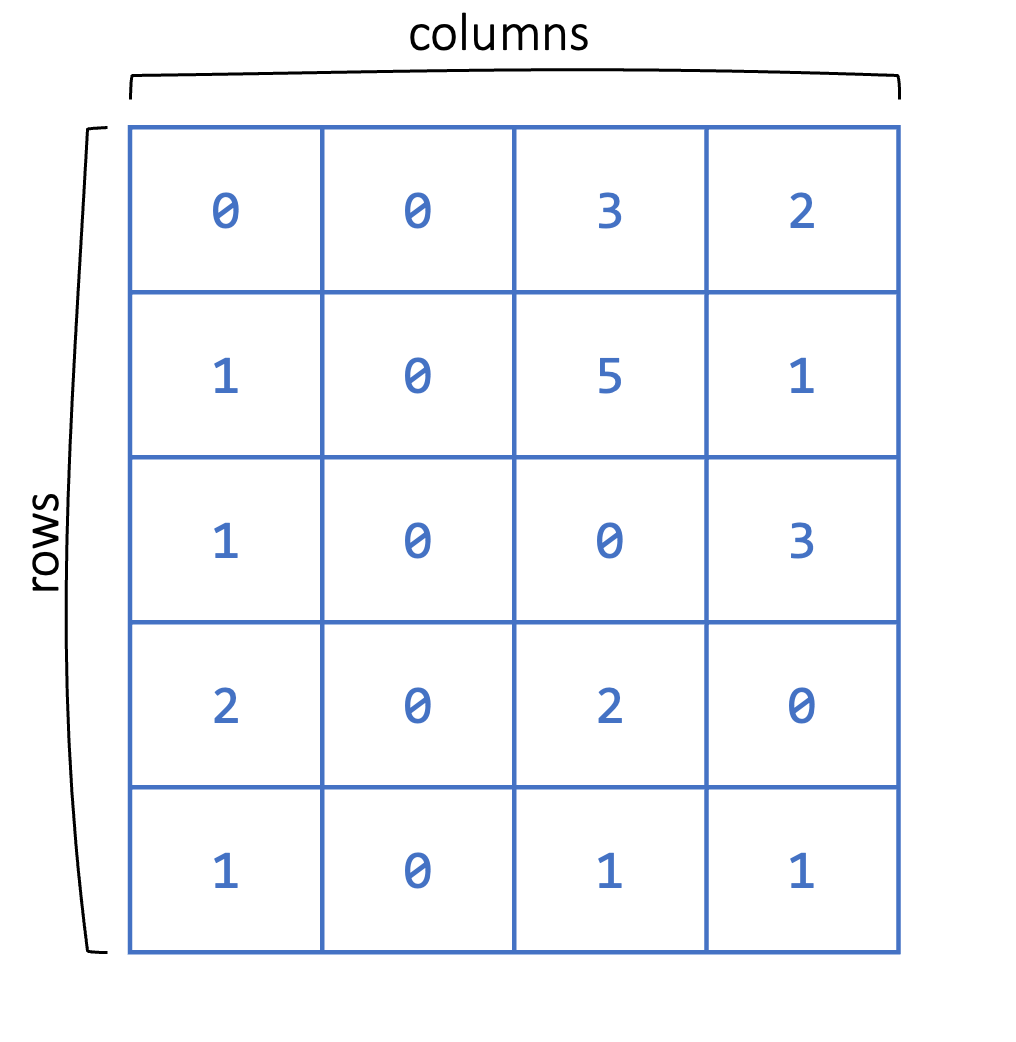
\includegraphics[width=0.4\textwidth,height=\textheight]{book/images/data_structures/matrix.png}

}

\caption{\label{fig-matrix}Matrix Example.}

\end{figure}%

In the following code, we create a matrix reporting the daily rainfall
over multiple weeks. We can create a matrix using the
\texttt{matrix(data,\ nrow,\ ncol,\ byrow)}\index{R functions!matrix()@\texttt{matrix()}}
function. This creates a \texttt{nrow} by \texttt{ncol} matrix from the
vector \texttt{data} values filling in by row if \texttt{byrow} is TRUE
and by column otherwise. Run the code. Then, change the last argument to
\texttt{byrow=FALSE} and see what happens to the values.

\begin{Shaded}
\begin{Highlighting}[]
\NormalTok{rainfall }\OtherTok{\textless{}{-}} \FunctionTok{matrix}\NormalTok{(}\FunctionTok{c}\NormalTok{(}\DecValTok{5}\NormalTok{, }\DecValTok{6}\NormalTok{, }\FloatTok{0.1}\NormalTok{, }\DecValTok{3}\NormalTok{, }\DecValTok{0}\NormalTok{, }\DecValTok{1}\NormalTok{, }\DecValTok{0}\NormalTok{, }\DecValTok{1}\NormalTok{, }\FloatTok{0.4}\NormalTok{, }\FloatTok{0.2}\NormalTok{, }
                     \FloatTok{0.5}\NormalTok{, }\FloatTok{0.3}\NormalTok{, }\DecValTok{0}\NormalTok{, }\DecValTok{0}\NormalTok{), }
                   \AttributeTok{ncol=}\DecValTok{7}\NormalTok{, }\AttributeTok{nrow=}\DecValTok{2}\NormalTok{, }\AttributeTok{byrow=}\ConstantTok{TRUE}\NormalTok{)}
\NormalTok{rainfall}
\CommentTok{\#\textgreater{}      [,1] [,2] [,3] [,4] [,5] [,6] [,7]}
\CommentTok{\#\textgreater{} [1,]    5  6.0  0.1  3.0  0.0    1    0}
\CommentTok{\#\textgreater{} [2,]    1  0.4  0.2  0.5  0.3    0    0}
\end{Highlighting}
\end{Shaded}

We can find the dimensions of a matrix using the
\texttt{nrow()}\index{R functions!nrow()@\texttt{nrow()}},
\texttt{ncol()}\index{R functions!ncol()@\texttt{ncol()}}, or
\texttt{dim()}\index{R functions!dim()@\texttt{dim()}} functions, which
return the number of rows, the number of columns, and both the number of
rows and columns, respectively.

\begin{Shaded}
\begin{Highlighting}[]
\FunctionTok{nrow}\NormalTok{(rainfall)}
\CommentTok{\#\textgreater{} [1] 2}
\FunctionTok{ncol}\NormalTok{(rainfall)}
\CommentTok{\#\textgreater{} [1] 7}
\FunctionTok{dim}\NormalTok{(rainfall)}
\CommentTok{\#\textgreater{} [1] 2 7}
\end{Highlighting}
\end{Shaded}

\subsection{\texorpdfstring{Indexing a Matrix
\index{matrices!indexing}}{Indexing a Matrix }}\label{indexing-a-matrix}

Since matrices are two-dimensional, a single value is indexed by both
its row number and its column number. This means that to access a subset
of values in a matrix, we need to provide row and column indices. In the
subsequent code, we access a single value in the first row and the
fourth column. The first value is always the row index and the second
value is always the column index.

\begin{Shaded}
\begin{Highlighting}[]
\NormalTok{rainfall[}\DecValTok{1}\NormalTok{, }\DecValTok{4}\NormalTok{]}
\CommentTok{\#\textgreater{} [1] 3}
\end{Highlighting}
\end{Shaded}

As before, we can also provide multiple indices to get multiple values.
In the subsequent example, we choose multiple columns, but we can also
choose multiple rows (or multiple rows and multiple columns).

\begin{Shaded}
\begin{Highlighting}[]
\NormalTok{rainfall[}\DecValTok{1}\NormalTok{, }\FunctionTok{c}\NormalTok{(}\DecValTok{4}\NormalTok{, }\DecValTok{5}\NormalTok{, }\DecValTok{7}\NormalTok{)]}
\CommentTok{\#\textgreater{} [1] 3 0 0}
\end{Highlighting}
\end{Shaded}

As with vectors, we can also use Booleans to index a matrix by providing
Boolean values for the rows and/or columns. Note that in the following
example we give a vector for the row indices and no values for the
columns. Since we did not specify any column indices, this selects all
of them.

\begin{Shaded}
\begin{Highlighting}[]
\NormalTok{rainfall[}\FunctionTok{c}\NormalTok{(}\ConstantTok{FALSE}\NormalTok{, }\ConstantTok{TRUE}\NormalTok{), ]}
\CommentTok{\#\textgreater{} [1] 1.0 0.4 0.2 0.5 0.3 0.0 0.0}
\end{Highlighting}
\end{Shaded}

Let's do the opposite and select some columns and all rows.

\begin{Shaded}
\begin{Highlighting}[]
\NormalTok{rainfall[ ,}\FunctionTok{c}\NormalTok{(}\ConstantTok{TRUE}\NormalTok{, }\ConstantTok{TRUE}\NormalTok{, }\ConstantTok{FALSE}\NormalTok{, }\ConstantTok{FALSE}\NormalTok{, }\ConstantTok{FALSE}\NormalTok{, }\ConstantTok{FALSE}\NormalTok{, }\ConstantTok{FALSE}\NormalTok{)]}
\CommentTok{\#\textgreater{}      [,1] [,2]}
\CommentTok{\#\textgreater{} [1,]    5  6.0}
\CommentTok{\#\textgreater{} [2,]    1  0.4}
\end{Highlighting}
\end{Shaded}

As with vectors, we can specify row names and column names
\index{matrices!names} to access entries instead of using indices. The
\texttt{colnames()}\index{R functions!colnames()@\texttt{colnames()}}
and \texttt{rownames()}
\index{R functions!rownames()@\texttt{rownames()}} functions allow us to
specify the column and row names, respectively.

\begin{Shaded}
\begin{Highlighting}[]
\FunctionTok{colnames}\NormalTok{(rainfall) }\OtherTok{\textless{}{-}} \FunctionTok{c}\NormalTok{(}\StringTok{"Monday"}\NormalTok{, }\StringTok{"Tuesday"}\NormalTok{, }\StringTok{"Wednesday"}\NormalTok{, }\StringTok{"Thursday"}\NormalTok{, }
                        \StringTok{"Friday"}\NormalTok{, }\StringTok{"Saturday"}\NormalTok{, }\StringTok{"Sunday"}\NormalTok{)}
\FunctionTok{rownames}\NormalTok{(rainfall) }\OtherTok{\textless{}{-}} \FunctionTok{c}\NormalTok{(}\StringTok{"Week1"}\NormalTok{, }\StringTok{"Week2"}\NormalTok{)}
\NormalTok{rainfall[}\StringTok{"Week1"}\NormalTok{, }\FunctionTok{c}\NormalTok{(}\StringTok{"Friday"}\NormalTok{,}\StringTok{"Saturday"}\NormalTok{)]}
\CommentTok{\#\textgreater{}   Friday Saturday }
\CommentTok{\#\textgreater{}        0        1}
\end{Highlighting}
\end{Shaded}

\subsection{\texorpdfstring{Modifying a Matrix
\index{matrices!modifying}}{Modifying a Matrix }}\label{modifying-a-matrix}

If we want to change the values in a matrix, we need to first index
those values and then assign them the new value(s). In the subsequent
code chunks, we change a single entry to be 3 and then update several
values to all be 0. Note that we do not provide multiple 0's on the
right-hand side, as R infers that all values should be set to 0.

\begin{Shaded}
\begin{Highlighting}[]
\NormalTok{rainfall[}\StringTok{"Week1"}\NormalTok{, }\StringTok{"Friday"}\NormalTok{] }\OtherTok{\textless{}{-}} \DecValTok{3}
\end{Highlighting}
\end{Shaded}

\begin{Shaded}
\begin{Highlighting}[]
\NormalTok{rainfall[}\StringTok{"Week1"}\NormalTok{, }\FunctionTok{c}\NormalTok{(}\StringTok{"Monday"}\NormalTok{, }\StringTok{"Tuesday"}\NormalTok{)] }\OtherTok{\textless{}{-}} \DecValTok{0}
\FunctionTok{print}\NormalTok{(rainfall)}
\CommentTok{\#\textgreater{}       Monday Tuesday Wednesday Thursday Friday Saturday Sunday}
\CommentTok{\#\textgreater{} Week1      0     0.0       0.1      3.0    3.0        1      0}
\CommentTok{\#\textgreater{} Week2      1     0.4       0.2      0.5    0.3        0      0}
\end{Highlighting}
\end{Shaded}

Further, we can append values to our matrix by adding rows or columns
through the \texttt{rbind()}\index{R functions!rbind()@\texttt{rbind()}}
and \texttt{cbind()}\index{R functions!cbind()@\texttt{cbind()}}
functions. The first function appends a row (or multiple rows) to a
matrix and the second appends a column (or multiple columns). Note that
in the following example I provide a row and column name when passing in
the additional data. If I hadn't specified these names, then those rows
and columns would not be named.

\begin{Shaded}
\begin{Highlighting}[]
\NormalTok{rainfall }\OtherTok{\textless{}{-}} \FunctionTok{rbind}\NormalTok{(rainfall, }\StringTok{"Week3"} \OtherTok{=} \FunctionTok{c}\NormalTok{(}\FloatTok{0.4}\NormalTok{, }\FloatTok{0.0}\NormalTok{, }\FloatTok{0.0}\NormalTok{, }\FloatTok{0.0}\NormalTok{, }\FloatTok{1.2}\NormalTok{, }\FloatTok{2.2}\NormalTok{, }
                                        \FloatTok{0.0}\NormalTok{))}
\NormalTok{rainfall }\OtherTok{\textless{}{-}} \FunctionTok{cbind}\NormalTok{(rainfall, }\StringTok{"Total"} \OtherTok{=} \FunctionTok{c}\NormalTok{(}\FloatTok{7.1}\NormalTok{, }\FloatTok{2.4}\NormalTok{, }\FloatTok{3.8}\NormalTok{))}
\FunctionTok{print}\NormalTok{(rainfall)}
\CommentTok{\#\textgreater{}       Monday Tuesday Wednesday Thursday Friday Saturday Sunday Total}
\CommentTok{\#\textgreater{} Week1    0.0     0.0       0.1      3.0    3.0      1.0      0   7.1}
\CommentTok{\#\textgreater{} Week2    1.0     0.4       0.2      0.5    0.3      0.0      0   2.4}
\CommentTok{\#\textgreater{} Week3    0.4     0.0       0.0      0.0    1.2      2.2      0   3.8}
\end{Highlighting}
\end{Shaded}

Here is an example where we bind two matrices by column. Note that
whenever we bind two matrices together, we have to be sure that their
dimensions are compatible and that they are of the same type.

\begin{Shaded}
\begin{Highlighting}[]
\NormalTok{A }\OtherTok{\textless{}{-}} \FunctionTok{matrix}\NormalTok{(}\FunctionTok{c}\NormalTok{(}\DecValTok{1}\NormalTok{, }\DecValTok{2}\NormalTok{, }\DecValTok{3}\NormalTok{, }\DecValTok{4}\NormalTok{), }\AttributeTok{nrow=}\DecValTok{2}\NormalTok{)}
\NormalTok{B }\OtherTok{\textless{}{-}} \FunctionTok{matrix}\NormalTok{(}\FunctionTok{c}\NormalTok{(}\DecValTok{5}\NormalTok{, }\DecValTok{6}\NormalTok{, }\DecValTok{7}\NormalTok{, }\DecValTok{8}\NormalTok{), }\AttributeTok{nrow=}\DecValTok{2}\NormalTok{)}
\NormalTok{C }\OtherTok{\textless{}{-}} \FunctionTok{cbind}\NormalTok{(A, B)}
\NormalTok{C}
\CommentTok{\#\textgreater{}      [,1] [,2] [,3] [,4]}
\CommentTok{\#\textgreater{} [1,]    1    3    5    7}
\CommentTok{\#\textgreater{} [2,]    2    4    6    8}
\end{Highlighting}
\end{Shaded}

As with vectors, most mathematical operators (\texttt{+}, \texttt{-},
\texttt{*}, \texttt{/}, etc.) are applied element-wise in R.

\begin{Shaded}
\begin{Highlighting}[]
\NormalTok{A}\SpecialCharTok{+}\NormalTok{B}
\CommentTok{\#\textgreater{}      [,1] [,2]}
\CommentTok{\#\textgreater{} [1,]    6   10}
\CommentTok{\#\textgreater{} [2,]    8   12}
\end{Highlighting}
\end{Shaded}

\begin{Shaded}
\begin{Highlighting}[]
\FunctionTok{exp}\NormalTok{(C)}
\CommentTok{\#\textgreater{}      [,1] [,2] [,3] [,4]}
\CommentTok{\#\textgreater{} [1,] 2.72 20.1  148 1097}
\CommentTok{\#\textgreater{} [2,] 7.39 54.6  403 2981}
\end{Highlighting}
\end{Shaded}

\subsection{Practice Question}\label{practice-question-1}

Create a \(3 \times 4\) matrix of all 1's using the \texttt{rep()} and
\texttt{matrix()} functions. Then select the first and third columns
using indexing which returns a \(3 \times 2\) matrix of all 1's.

\begin{Shaded}
\begin{Highlighting}[]
\CommentTok{\# Insert your solution here:}
\end{Highlighting}
\end{Shaded}

\section{\texorpdfstring{Data Frames
\index{data frames}}{Data Frames }}\label{data-frames}

Matrices can store data like the rainfall data, where everything is of
the same type. However, if we want to capture more complex data records,
we also want to allow for different measurement types: this is where
data frames come in. A data frame is like a matrix in that data frames
are two-dimensional, but unlike matrices, data frames allow for each
column to be a different type (see Figure~\ref{fig-dataframe}). In this
case, each row corresponds to a single data entry (or observation) and
each column corresponds to a different variable.

\begin{figure}

\centering{

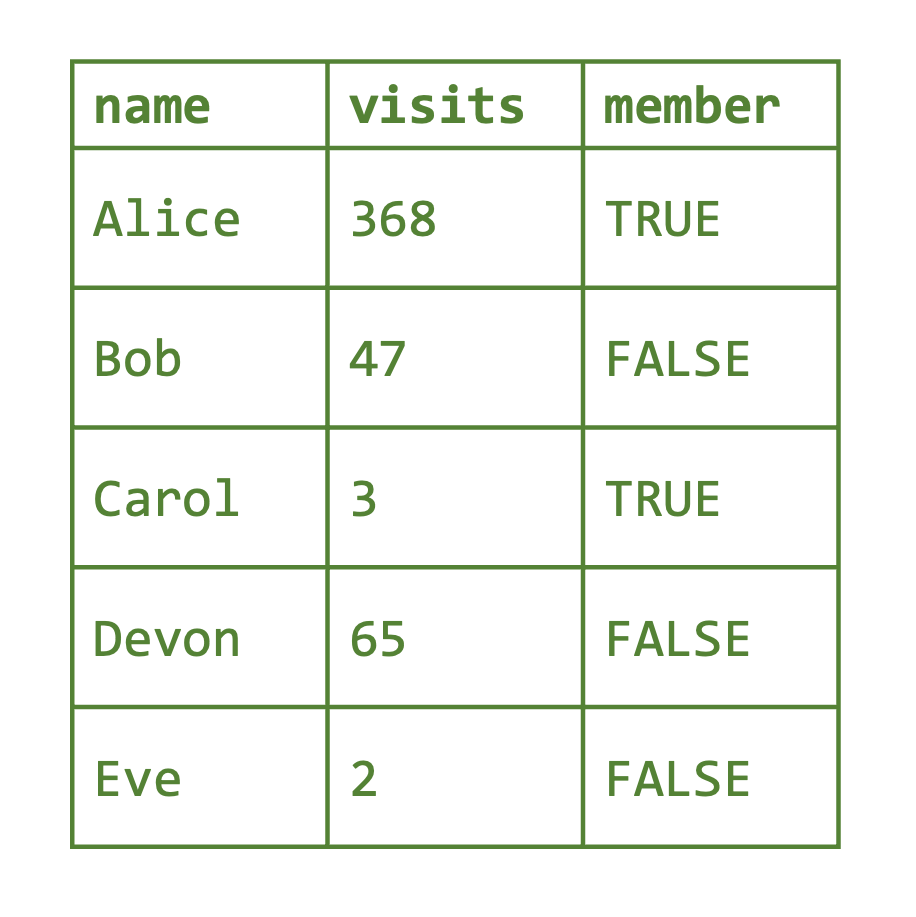
\includegraphics[width=0.4\textwidth,height=\textheight]{book/images/data_structures/dataframe.png}

}

\caption{\label{fig-dataframe}Data Frame Example.}

\end{figure}%

For example, suppose that, for every day in a study, we want to record
the temperature, rainfall, and day of the week. Temperature and rainfall
can be numeric values, but day of the week is character type. We create
a data frame using the
\texttt{data.frame()}\index{R functions!data.frame()@\texttt{data.frame()}}
function. Note that I am providing column names for each vector
(column).

The \texttt{head()}\index{R functions!head()@\texttt{head()}} function
prints the first six rows of a data frame (to avoid printing very large
datasets). In our case, all the data is shown because we only created
four rows. The column names are displayed as well as their type. By
contrast, the \texttt{tail()}\index{R functions!tail()@\texttt{tail()}}
function prints the last six rows of a data frame.

\begin{Shaded}
\begin{Highlighting}[]
\NormalTok{weather\_data }\OtherTok{\textless{}{-}} \FunctionTok{data.frame}\NormalTok{(}\AttributeTok{day\_of\_week =} \FunctionTok{c}\NormalTok{(}\StringTok{"Monday"}\NormalTok{, }\StringTok{"Tuesday"}\NormalTok{,}
                                           \StringTok{"Wednesday"}\NormalTok{, }\StringTok{"Monday"}\NormalTok{), }
                           \AttributeTok{temp =} \FunctionTok{c}\NormalTok{(}\DecValTok{70}\NormalTok{, }\DecValTok{62}\NormalTok{, }\DecValTok{75}\NormalTok{, }\DecValTok{50}\NormalTok{), }
                           \AttributeTok{rain =} \FunctionTok{c}\NormalTok{(}\DecValTok{5}\NormalTok{, }\FloatTok{0.1}\NormalTok{, }\FloatTok{0.0}\NormalTok{, }\FloatTok{0.5}\NormalTok{))}
\FunctionTok{head}\NormalTok{(weather\_data)}
\CommentTok{\#\textgreater{}   day\_of\_week temp rain}
\CommentTok{\#\textgreater{} 1      Monday   70  5.0}
\CommentTok{\#\textgreater{} 2     Tuesday   62  0.1}
\CommentTok{\#\textgreater{} 3   Wednesday   75  0.0}
\CommentTok{\#\textgreater{} 4      Monday   50  0.5}
\end{Highlighting}
\end{Shaded}

The \texttt{dim()}\index{R functions!dim()@\texttt{dim()}},
\texttt{nrow()}\index{R functions!nrow()@\texttt{nrow()}}, and
\texttt{ncol()}\index{R functions!ncol()@\texttt{ncol()}} functions
return the dimensions, number of rows, and number of columns of a data
frame, respectively.

\begin{Shaded}
\begin{Highlighting}[]
\FunctionTok{dim}\NormalTok{(weather\_data)}
\CommentTok{\#\textgreater{} [1] 4 3}
\FunctionTok{nrow}\NormalTok{(weather\_data)}
\CommentTok{\#\textgreater{} [1] 4}
\FunctionTok{ncol}\NormalTok{(weather\_data)}
\CommentTok{\#\textgreater{} [1] 3}
\end{Highlighting}
\end{Shaded}

The column names can be found (or assigned) using the
\texttt{colnames()}\index{R functions!colnames()@\texttt{colnames()}} or
\texttt{names()}\index{R functions!names()@\texttt{names()}} function.
These were specified when I created the data. On the other hand, the row
names are currently the indices.

\begin{Shaded}
\begin{Highlighting}[]
\FunctionTok{colnames}\NormalTok{(weather\_data)}
\CommentTok{\#\textgreater{} [1] "day\_of\_week" "temp"        "rain"}
\FunctionTok{rownames}\NormalTok{(weather\_data)}
\CommentTok{\#\textgreater{} [1] "1" "2" "3" "4"}
\FunctionTok{names}\NormalTok{(weather\_data)}
\CommentTok{\#\textgreater{} [1] "day\_of\_week" "temp"        "rain"}
\end{Highlighting}
\end{Shaded}

We update the row names to be more informative as with a matrix using
the
\texttt{rownames()}\index{R functions!rownames()@\texttt{rownames()}}
function.

\begin{Shaded}
\begin{Highlighting}[]
\FunctionTok{rownames}\NormalTok{(weather\_data) }\OtherTok{\textless{}{-}} \FunctionTok{c}\NormalTok{(}\StringTok{"6/1"}\NormalTok{, }\StringTok{"6/2"}\NormalTok{, }\StringTok{"6/3"}\NormalTok{, }\StringTok{"6/8"}\NormalTok{)}
\FunctionTok{head}\NormalTok{(weather\_data)}
\CommentTok{\#\textgreater{}     day\_of\_week temp rain}
\CommentTok{\#\textgreater{} 6/1      Monday   70  5.0}
\CommentTok{\#\textgreater{} 6/2     Tuesday   62  0.1}
\CommentTok{\#\textgreater{} 6/3   Wednesday   75  0.0}
\CommentTok{\#\textgreater{} 6/8      Monday   50  0.5}
\end{Highlighting}
\end{Shaded}

\subsection{\texorpdfstring{Indexing a Data Frame
\index{data frames!indexing}}{Indexing a Data Frame }}\label{indexing-a-data-frame}

We can select elements of the data frame using its indices in the same
way as we did with matrices. In the subsequent code, we access a single
value and then a subset of our data frame. The subset returned is itself
a data frame. Note that the second line returns a data frame.

\begin{Shaded}
\begin{Highlighting}[]
\NormalTok{weather\_data[}\DecValTok{1}\NormalTok{, }\DecValTok{2}\NormalTok{]}
\CommentTok{\#\textgreater{} [1] 70}
\NormalTok{weather\_data[}\DecValTok{1}\NormalTok{, }\FunctionTok{c}\NormalTok{(}\StringTok{"day\_of\_week"}\NormalTok{, }\StringTok{"temp"}\NormalTok{)]}
\CommentTok{\#\textgreater{}     day\_of\_week temp}
\CommentTok{\#\textgreater{} 6/1      Monday   70}
\end{Highlighting}
\end{Shaded}

Another useful way to access the columns of a data frame is by using the
\texttt{\$} accessor and the column name.

\begin{Shaded}
\begin{Highlighting}[]
\NormalTok{weather\_data}\SpecialCharTok{$}\NormalTok{day\_of\_week}
\CommentTok{\#\textgreater{} [1] "Monday"    "Tuesday"   "Wednesday" "Monday"}
\NormalTok{weather\_data}\SpecialCharTok{$}\NormalTok{temp}
\CommentTok{\#\textgreater{} [1] 70 62 75 50}
\end{Highlighting}
\end{Shaded}

The column \texttt{day\_of\_week} is a categorical column, but it can
only take on a limited number of values. For this kind of column, it is
often useful to convert that column to a factor as we did before.

\begin{Shaded}
\begin{Highlighting}[]
\NormalTok{weather\_data}\SpecialCharTok{$}\NormalTok{day\_of\_week }\OtherTok{\textless{}{-}} \FunctionTok{factor}\NormalTok{(weather\_data}\SpecialCharTok{$}\NormalTok{day\_of\_week)}
\FunctionTok{levels}\NormalTok{(weather\_data}\SpecialCharTok{$}\NormalTok{day\_of\_week)}
\CommentTok{\#\textgreater{} [1] "Monday"    "Tuesday"   "Wednesday"}
\end{Highlighting}
\end{Shaded}

\subsection{\texorpdfstring{Modifying a Data Frame
\index{data frames!modifying}}{Modifying a Data Frame }}\label{modifying-a-data-frame}

As with matrices, we can change values in a data frame by indexing those
entries.

\begin{Shaded}
\begin{Highlighting}[]
\NormalTok{weather\_data[}\DecValTok{1}\NormalTok{, }\StringTok{"rain"}\NormalTok{] }\OtherTok{\textless{}{-}} \FloatTok{2.2}
\NormalTok{weather\_data}
\CommentTok{\#\textgreater{}     day\_of\_week temp rain}
\CommentTok{\#\textgreater{} 6/1      Monday   70  2.2}
\CommentTok{\#\textgreater{} 6/2     Tuesday   62  0.1}
\CommentTok{\#\textgreater{} 6/3   Wednesday   75  0.0}
\CommentTok{\#\textgreater{} 6/8      Monday   50  0.5}
\end{Highlighting}
\end{Shaded}

The \texttt{rbind()}\index{R functions!rbind()@\texttt{rbind()}}
functions and
\texttt{cbind()}\index{R functions!cbind()@\texttt{cbind()}} functions
also work for data frames in the same way as for matrices. However,
another way to add a column is to directly use the
\texttt{\$}\index{\$ accessor} accessor. We add a categorical column
called \texttt{aq\_warning}, indicating whether there was an air quality
warning that day.

\begin{Shaded}
\begin{Highlighting}[]
\NormalTok{weather\_data}\SpecialCharTok{$}\NormalTok{aq\_warning }\OtherTok{\textless{}{-}} \FunctionTok{as.factor}\NormalTok{(}\FunctionTok{c}\NormalTok{(}\DecValTok{1}\NormalTok{, }\DecValTok{0}\NormalTok{, }\DecValTok{0}\NormalTok{, }\DecValTok{0}\NormalTok{))}
\NormalTok{weather\_data}
\CommentTok{\#\textgreater{}     day\_of\_week temp rain aq\_warning}
\CommentTok{\#\textgreater{} 6/1      Monday   70  2.2          1}
\CommentTok{\#\textgreater{} 6/2     Tuesday   62  0.1          0}
\CommentTok{\#\textgreater{} 6/3   Wednesday   75  0.0          0}
\CommentTok{\#\textgreater{} 6/8      Monday   50  0.5          0}
\end{Highlighting}
\end{Shaded}

\subsection{Practice Question}\label{practice-question-2}

Add a column to \texttt{weather\_data} called
\texttt{air\_quality\_index} using the \texttt{rep()} function so that
all values are \texttt{NA} \index{NA values} (the missing value in R).
Then, index the second value of this column and set the value to be 57.
The result should look like Figure~\ref{fig-daily-air-quality}.

\begin{figure}

\centering{

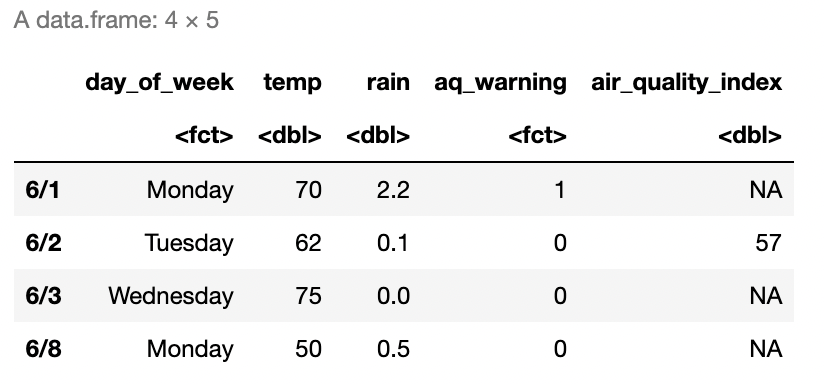
\includegraphics[width=0.7\textwidth,height=\textheight]{book/images/data_structures/daily-air-quality.png}

}

\caption{\label{fig-daily-air-quality}Air Quality Data.}

\end{figure}%

\begin{Shaded}
\begin{Highlighting}[]
\CommentTok{\# Insert your solution here:}
\end{Highlighting}
\end{Shaded}

\section{\texorpdfstring{Lists \index{lists}}{Lists }}\label{lists}

A data frame is actually a special type of another data structure called
a \textbf{list}, which is a collection of objects under the same name.
These objects can be vectors, matrices, data frames, or even other
lists! There does not have to be any relation in size, type, or other
attribute between different members of the list. We create an example
list using the \texttt{list()}
\index{R functions!list()@\texttt{list()}} function, which takes in a
series of objects. What are the types of each element of the following
list?

\begin{Shaded}
\begin{Highlighting}[]
\NormalTok{ex\_list }\OtherTok{\textless{}{-}} \FunctionTok{list}\NormalTok{(}\StringTok{"John"}\NormalTok{, }\FunctionTok{c}\NormalTok{(}\StringTok{"ibuprofen"}\NormalTok{, }\StringTok{"metformin"}\NormalTok{), }
                \FunctionTok{c}\NormalTok{(}\DecValTok{136}\NormalTok{, }\DecValTok{142}\NormalTok{, }\DecValTok{159}\NormalTok{))}
\FunctionTok{print}\NormalTok{(ex\_list)}
\CommentTok{\#\textgreater{} [[1]]}
\CommentTok{\#\textgreater{} [1] "John"}
\CommentTok{\#\textgreater{} }
\CommentTok{\#\textgreater{} [[2]]}
\CommentTok{\#\textgreater{} [1] "ibuprofen" "metformin"}
\CommentTok{\#\textgreater{} }
\CommentTok{\#\textgreater{} [[3]]}
\CommentTok{\#\textgreater{} [1] 136 142 159}
\end{Highlighting}
\end{Shaded}

We can access each element using the index\index{lists!indexing}. Note
unlike indexing vectors, using single brackets will return another list
which is a sub-list containing the object at that index.

\begin{Shaded}
\begin{Highlighting}[]
\FunctionTok{print}\NormalTok{(}\FunctionTok{class}\NormalTok{(ex\_list[}\DecValTok{2}\NormalTok{]))}
\CommentTok{\#\textgreater{} [1] "list"}
\NormalTok{ex\_list[}\DecValTok{2}\NormalTok{]}
\CommentTok{\#\textgreater{} [[1]]}
\CommentTok{\#\textgreater{} [1] "ibuprofen" "metformin"}
\end{Highlighting}
\end{Shaded}

We can access the actual numeric vector at this index using double
brackets.

\begin{Shaded}
\begin{Highlighting}[]
\NormalTok{ex\_list[[}\DecValTok{2}\NormalTok{]]}
\CommentTok{\#\textgreater{} [1] "ibuprofen" "metformin"}
\end{Highlighting}
\end{Shaded}

More often, however, it is useful to name the elements of the list for
easier access\index{lists!naming}. Let's create this list again but,
this time, give names to each object.

\begin{Shaded}
\begin{Highlighting}[]
\NormalTok{ex\_list }\OtherTok{\textless{}{-}} \FunctionTok{list}\NormalTok{(}\AttributeTok{name=}\StringTok{"John"}\NormalTok{, }
                \AttributeTok{medications =} \FunctionTok{c}\NormalTok{(}\StringTok{"ibuprofen"}\NormalTok{, }\StringTok{"metformin"}\NormalTok{), }
                \AttributeTok{past\_weights =} \FunctionTok{c}\NormalTok{(}\DecValTok{136}\NormalTok{, }\DecValTok{142}\NormalTok{, }\DecValTok{159}\NormalTok{))}
\FunctionTok{print}\NormalTok{(ex\_list)}
\CommentTok{\#\textgreater{} $name}
\CommentTok{\#\textgreater{} [1] "John"}
\CommentTok{\#\textgreater{} }
\CommentTok{\#\textgreater{} $medications}
\CommentTok{\#\textgreater{} [1] "ibuprofen" "metformin"}
\CommentTok{\#\textgreater{} }
\CommentTok{\#\textgreater{} $past\_weights}
\CommentTok{\#\textgreater{} [1] 136 142 159}
\NormalTok{ex\_list}\SpecialCharTok{$}\NormalTok{medications}
\CommentTok{\#\textgreater{} [1] "ibuprofen" "metformin"}
\end{Highlighting}
\end{Shaded}

To edit a list, we can use indexing to access different objects in the
list and then assign them to new values. Additionally, we can add
objects to the list using the \texttt{\$} accessor\index{\$ accessor}.

\begin{Shaded}
\begin{Highlighting}[]
\NormalTok{ex\_list}\SpecialCharTok{$}\NormalTok{supplements }\OtherTok{\textless{}{-}} \FunctionTok{c}\NormalTok{(}\StringTok{"vitamin D"}\NormalTok{, }\StringTok{"biotin"}\NormalTok{)}
\NormalTok{ex\_list}\SpecialCharTok{$}\NormalTok{supplements[}\DecValTok{2}\NormalTok{] }\OtherTok{\textless{}{-}} \StringTok{"collagen"}
\NormalTok{ex\_list}
\CommentTok{\#\textgreater{} $name}
\CommentTok{\#\textgreater{} [1] "John"}
\CommentTok{\#\textgreater{} }
\CommentTok{\#\textgreater{} $medications}
\CommentTok{\#\textgreater{} [1] "ibuprofen" "metformin"}
\CommentTok{\#\textgreater{} }
\CommentTok{\#\textgreater{} $past\_weights}
\CommentTok{\#\textgreater{} [1] 136 142 159}
\CommentTok{\#\textgreater{} }
\CommentTok{\#\textgreater{} $supplements}
\CommentTok{\#\textgreater{} [1] "vitamin D" "collagen"}
\end{Highlighting}
\end{Shaded}

\section{Exercises}\label{exercises}

\begin{enumerate}
\def\labelenumi{\arabic{enumi}.}
\tightlist
\item
  Recreate the data frame in Figure~\ref{fig-city-air-quality} in R,
  where \texttt{temperature} and \texttt{co2} represent the average
  temperature in Fahrenheit and the average \(\text{CO}_2\)
  concentrations in \(\text{mg}/\text{m}^3\) for the month of January
  2008, and name it \texttt{city\_air\_quality}.
\end{enumerate}

\begin{figure}

\centering{

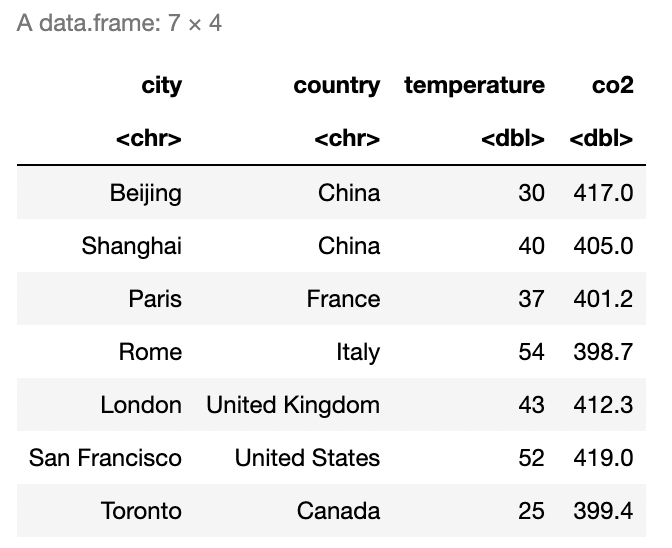
\includegraphics[width=0.7\textwidth,height=\textheight]{book/images/data_structures/city-air-quality.png}

}

\caption{\label{fig-city-air-quality}City Air Quality Data.}

\end{figure}%

\begin{enumerate}
\def\labelenumi{\arabic{enumi}.}
\setcounter{enumi}{1}
\item
  Create a character vector named \texttt{precipitation} with entries
  \texttt{Yes} or \texttt{No} indicating whether or not there was more
  precipitation than average in January 2008 in these cities (you can
  make this information up yourself). Then, append this vector to the
  \texttt{city\_air\_quality} data frame as a new column.
\item
  Convert the categorical column \texttt{precipitation} to a factor.
  Then, add a row to the data frame \texttt{city\_air\_quality} using
  the \texttt{rbind()} function to match
  Figure~\ref{fig-city-air-quality-2}.
\end{enumerate}

\begin{figure}

\centering{

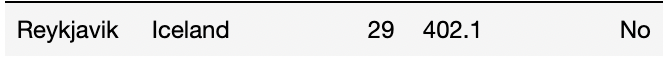
\includegraphics[width=0.7\textwidth,height=\textheight]{book/images/data_structures/city-air-quality-newrow.png}

}

\caption{\label{fig-city-air-quality-2}Updated City Air Quality Data.}

\end{figure}%

\begin{enumerate}
\def\labelenumi{\arabic{enumi}.}
\setcounter{enumi}{3}
\tightlist
\item
  Use single square brackets to access the precipitation and
  \(\text{CO}_2\) concentration entries for San Francisco and Paris in
  your data frame. Then, create a list \texttt{city\_list} which
  contains two lists, one for San Francisco and one for Paris, where
  each inner list contains the city name, precipitation, and
  \(\text{CO}_2\) concentration information for that city.
\end{enumerate}

\chapter{Working with Data Files in R}\label{sec-data-files}

In this chapter, we work with data in R. To start, we need to load our
data into R; this requires identifying the type of data file
\index{data file} we have (e.g., .csv, .xlsx, .dta, .txt) and finding
the appropriate function to load in the data. This creates a data frame
object containing the information from the file. After demonstrating how
to load in such data, this chapter shows you how to find information
about data columns, including finding missing values, summarizing
columns, and subsetting the data. Additionally, we look at how to create
new columns through some simple transformations.

In this chapter and all future chapters, we load in the required
libraries at the start of the chapter; for example, in this particular
chapter, we need a single package \textbf{HDSinRdata}
\index{R packages!HDSinRdata} that contains the sample datasets used in
this book.

\begin{Shaded}
\begin{Highlighting}[]
\FunctionTok{library}\NormalTok{(HDSinRdata)}
\end{Highlighting}
\end{Shaded}

\section{\texorpdfstring{Importing and Exporting Data
\index{importing data}
\index{exporting data}}{Importing and Exporting Data  }}\label{importing-and-exporting-data}

The data we use in this chapter contains information about patients who
visited one of the University of Pittsburgh's seven pain management
clinics. This includes patient-reported pain assessments using the
Collaborative Health Outcomes Information Registry (CHOIR) at baseline
and at a 3-month follow-up (Alter et al. 2021). You can use the help
operator \texttt{?pain} to learn more about the source of this data and
to read its column descriptions\index{Datasets!pain@\texttt{pain}}.
Since this data is available in our R package, we can use the
\texttt{data()}\index{R functions!data()@\texttt{data()}} function to
load this data into our environment. Note that this data has 21,659 rows
and 92 columns.

\begin{Shaded}
\begin{Highlighting}[]
\FunctionTok{data}\NormalTok{(pain)}
\FunctionTok{dim}\NormalTok{(pain)}
\CommentTok{\#\textgreater{} [1] 21659    92}
\end{Highlighting}
\end{Shaded}

In general, the data you will be using is not available in R packages
and will instead exist in one or more data files on your personal
computer. In order to load in this data to R, you need to use the
function that corresponds to the file type you have. For example, you
can load a .csv file \index{data files!.csv} using the
\texttt{read.csv()}\index{R functions!read.csv()@\texttt{read.csv()}}
function in base R or using the
\texttt{read\_csv()}\index{R functions!read\textunderscore csv()@\texttt{read\textunderscore csv()}}
function from the \textbf{readr} package\index{R packages!readr}, both
of which were shown in Chapter~\ref{sec-intro-to-r}. As an example, we
load the \texttt{fake\_names.csv} dataset using both of these functions.
Looking at the print output, we can see that there is a slight
difference in the data structure and data types storing the data between
these two functions. The function \texttt{read.csv()} loads the data as
a data frame, whereas the function \texttt{read\_csv()} loads the data
as a \texttt{spec\_tbl\_df}, a special type of data frame called a
\textbf{tibble}\index{tibble} that is used by the \textbf{tidyverse}
packages\index{R packages!tidyverse}. We cover this data structure in
more detail in Chapter~\ref{sec-transformations-summaries}. For now,
note that you can use either function to read in a .csv file.

\begin{Shaded}
\begin{Highlighting}[]
\FunctionTok{read.csv}\NormalTok{(}\StringTok{"data/fake\_names.csv"}\NormalTok{)}
\CommentTok{\#\textgreater{}                  Name Age     DOB            City State}
\CommentTok{\#\textgreater{} 1           Ken Irwin  37 6/28/85      Providence    RI}
\CommentTok{\#\textgreater{} 2 Delores Whittington  56 4/28/67      Smithfield    RI}
\CommentTok{\#\textgreater{} 3       Daniel Hughes  41 5/22/82      Providence    RI}
\CommentTok{\#\textgreater{} 4         Carlos Fain  83  2/2/40          Warren    RI}
\CommentTok{\#\textgreater{} 5        James Alford  67 2/23/56 East Providence    RI}
\CommentTok{\#\textgreater{} 6        Ruth Alvarez  34 9/22/88      Providence    RI}
\end{Highlighting}
\end{Shaded}

\begin{Shaded}
\begin{Highlighting}[]
\NormalTok{readr}\SpecialCharTok{::}\FunctionTok{read\_csv}\NormalTok{(}\StringTok{"data/fake\_names.csv"}\NormalTok{, }\AttributeTok{show\_col\_types=}\ConstantTok{FALSE}\NormalTok{)}
\CommentTok{\#\textgreater{} \# A tibble: 6 x 5}
\CommentTok{\#\textgreater{}   Name                  Age DOB     City            State}
\CommentTok{\#\textgreater{}   \textless{}chr\textgreater{}               \textless{}dbl\textgreater{} \textless{}chr\textgreater{}   \textless{}chr\textgreater{}           \textless{}chr\textgreater{}}
\CommentTok{\#\textgreater{} 1 Ken Irwin              37 6/28/85 Providence      RI   }
\CommentTok{\#\textgreater{} 2 Delores Whittington    56 4/28/67 Smithfield      RI   }
\CommentTok{\#\textgreater{} 3 Daniel Hughes          41 5/22/82 Providence      RI   }
\CommentTok{\#\textgreater{} 4 Carlos Fain            83 2/2/40  Warren          RI   }
\CommentTok{\#\textgreater{} 5 James Alford           67 2/23/56 East Providence RI   }
\CommentTok{\#\textgreater{} 6 Ruth Alvarez           34 9/22/88 Providence      RI}
\end{Highlighting}
\end{Shaded}

In addition to loading data into R, you may also want to save data from
R into a data file you can access later or share with others. To write a
data frame \index{exporting data} from R to a .csv file, you can use the
\texttt{write.csv()}
\index{R functions!write.csv()@\texttt{write.csv()}} function. This
function has three key arguments: the first argument is the data frame
in R that you want to write to a file, the second argument is the file
name or the full file path where you want to write the data, and the
third argument is whether or not you want to include the row names as an
extra column. In this case, we do not include row names. If you do not
specify a file path, R saves the file in our current working directory.

\begin{Shaded}
\begin{Highlighting}[]
\NormalTok{df }\OtherTok{\textless{}{-}} \FunctionTok{data.frame}\NormalTok{(}\AttributeTok{x =} \FunctionTok{c}\NormalTok{( }\DecValTok{1}\NormalTok{, }\DecValTok{0}\NormalTok{, }\DecValTok{1}\NormalTok{), }\AttributeTok{y =} \FunctionTok{c}\NormalTok{(}\StringTok{"A"}\NormalTok{, }\StringTok{"B"}\NormalTok{, }\StringTok{"C"}\NormalTok{))}
\FunctionTok{write.csv}\NormalTok{(df, }\StringTok{"data/test.csv"}\NormalTok{, }\AttributeTok{row.names=}\ConstantTok{FALSE}\NormalTok{)}
\end{Highlighting}
\end{Shaded}

If your data is not in a .csv file, you may need to use another package
to read in the file. The two most common packages are the
\textbf{readxl} package\index{R packages!readxl} (Wickham and Bryan
2023), which makes it easy to read in Excel files, and the
\textbf{haven} package\index{R packages!haven} (Wickham, Miller, and
Smith 2023), which can import SAS, SPSS, and Stata files. For each
function, you need to specify the file path to the data file.

\begin{itemize}
\item
  \textbf{Tab-Delimited Files}: You can read in a tab-separated .txt
  \index{data files!.txt} file using the
  \texttt{read.delim()}\index{R functions!read.delim()@\texttt{read.delim()}}
  function in base R.
\item
  \textbf{Excel Files}: You can read in a .xls \index{data files!.xls}
  or .xlsx file \index{data files!.xlsx} using
  \texttt{readxl::read\_excel()}\index{R functions!read\textunderscore excel()@\texttt{read\textunderscore excel()}},
  which allows you to specify a sheet and/or cell range within a file
  (e.g.,
  \texttt{read\_excel(\textquotesingle{}test.xlsx\textquotesingle{},\ sheet="Sheet1")}).
\item
  \textbf{SAS}:
  \texttt{haven::read\_sas()}\index{R functions!read\textunderscore sas()@\texttt{read\textunderscore sas()}}
  reads in .sas7bdat\index{data files!.sas7bdat} or .sas7bcat
  files\index{data files!.sas7bcat}, \texttt{haven::read\_xpt()}
  \index{R functions!read\textunderscore xpt()@\texttt{read\textunderscore xpt()}}
  reads in SAS transport files.
\item
  \textbf{Stata}:
  \texttt{haven::read\_dta()}\index{R functions!read\textunderscore dta()@\texttt{read\textunderscore dta()}}
  reads in .dta\index{data files!.dta} files.
\item
  \textbf{SPSS}:
  \texttt{haven::read\_spss()}\index{R functions!read\textunderscore spss()@\texttt{read\textunderscore spss()}}
  reads in .spss\index{data files!.spss} files.
\end{itemize}

\section{Summarizing and Creating Data
Columns}\label{summarizing-and-creating-data-columns}

We now look at the data we have loaded into the data frame called
\texttt{pain}. We use the
\texttt{head()}\index{R functions!head()@\texttt{head()}} function to
print the first six rows. However, note that we have so many columns
that not all of the columns are displayed! For those that are displayed,
we can see the data type for each column under the column name. For
example, we can see that the column \texttt{PATIENT\_NUM} is a numeric
column of type \texttt{dbl}. Because patients identification numbers are
technically nominal in nature, we might consider whether we should make
convert this column to a factor or a character representation later on.
We can use the
\texttt{names()}\index{R functions!names()@\texttt{names()}} function to
print all the column names. Note that columns \texttt{X101} to
\texttt{X238} correspond to numbers on a body pain map (see the data
documentation for the image of this map). Each of these columns has a 1
if the patient indicated that they have pain in that corresponding body
part and a 0 otherwise.

\begin{Shaded}
\begin{Highlighting}[]
\FunctionTok{head}\NormalTok{(pain)}
\CommentTok{\#\textgreater{} \# A tibble: 6 x 92}
\CommentTok{\#\textgreater{}   PATIENT\_NUM  X101  X102  X103  X104  X105  X106  X107  X108  X109}
\CommentTok{\#\textgreater{}         \textless{}dbl\textgreater{} \textless{}dbl\textgreater{} \textless{}dbl\textgreater{} \textless{}dbl\textgreater{} \textless{}dbl\textgreater{} \textless{}dbl\textgreater{} \textless{}dbl\textgreater{} \textless{}dbl\textgreater{} \textless{}dbl\textgreater{} \textless{}dbl\textgreater{}}
\CommentTok{\#\textgreater{} 1       13118     0     0     0     0     0     0     0     0     0}
\CommentTok{\#\textgreater{} 2       21384     0     0     0     0     0     0     0     0     0}
\CommentTok{\#\textgreater{} 3        6240     0     0     0     0     0     0     0     0     0}
\CommentTok{\#\textgreater{} 4        1827     0     0     0     0     0     0     0     0     0}
\CommentTok{\#\textgreater{} 5       11309     0     0     0     0     0     0     0     0     0}
\CommentTok{\#\textgreater{} 6       11093     0     0     0     0     0     0     0     0     0}
\CommentTok{\#\textgreater{} \# i 82 more variables: X110 \textless{}dbl\textgreater{}, X111 \textless{}dbl\textgreater{}, X112 \textless{}dbl\textgreater{}, X113 \textless{}dbl\textgreater{},}
\CommentTok{\#\textgreater{} \#   X114 \textless{}dbl\textgreater{}, X115 \textless{}dbl\textgreater{}, X116 \textless{}dbl\textgreater{}, X117 \textless{}dbl\textgreater{}, X118 \textless{}dbl\textgreater{},}
\CommentTok{\#\textgreater{} \#   X119 \textless{}dbl\textgreater{}, X120 \textless{}dbl\textgreater{}, X121 \textless{}dbl\textgreater{}, X122 \textless{}dbl\textgreater{}, X123 \textless{}dbl\textgreater{},}
\CommentTok{\#\textgreater{} \#   X124 \textless{}dbl\textgreater{}, X125 \textless{}dbl\textgreater{}, X126 \textless{}dbl\textgreater{}, X127 \textless{}dbl\textgreater{}, X128 \textless{}dbl\textgreater{},}
\CommentTok{\#\textgreater{} \#   X129 \textless{}dbl\textgreater{}, X130 \textless{}dbl\textgreater{}, X131 \textless{}dbl\textgreater{}, X132 \textless{}dbl\textgreater{}, X133 \textless{}dbl\textgreater{},}
\CommentTok{\#\textgreater{} \#   X134 \textless{}dbl\textgreater{}, X135 \textless{}dbl\textgreater{}, X136 \textless{}dbl\textgreater{}, X201 \textless{}dbl\textgreater{}, X202 \textless{}dbl\textgreater{},}
\CommentTok{\#\textgreater{} \#   X203 \textless{}dbl\textgreater{}, X204 \textless{}dbl\textgreater{}, X205 \textless{}dbl\textgreater{}, X206 \textless{}dbl\textgreater{}, X207 \textless{}dbl\textgreater{}, ...}
\FunctionTok{names}\NormalTok{(pain)}
\CommentTok{\#\textgreater{}  [1] "PATIENT\_NUM"                     }
\CommentTok{\#\textgreater{}  [2] "X101"                            }
\CommentTok{\#\textgreater{}  [3] "X102"                            }
\CommentTok{\#\textgreater{}  [4] "X103"                            }
\CommentTok{\#\textgreater{}  [5] "X104"                            }
\CommentTok{\#\textgreater{}  [6] "X105"                            }
\CommentTok{\#\textgreater{}  [7] "X106"                            }
\CommentTok{\#\textgreater{}  [8] "X107"                            }
\CommentTok{\#\textgreater{}  [9] "X108"                            }
\CommentTok{\#\textgreater{} [10] "X109"                            }
\CommentTok{\#\textgreater{} [11] "X110"                            }
\CommentTok{\#\textgreater{} [12] "X111"                            }
\CommentTok{\#\textgreater{} [13] "X112"                            }
\CommentTok{\#\textgreater{} [14] "X113"                            }
\CommentTok{\#\textgreater{} [15] "X114"                            }
\CommentTok{\#\textgreater{} [16] "X115"                            }
\CommentTok{\#\textgreater{} [17] "X116"                            }
\CommentTok{\#\textgreater{} [18] "X117"                            }
\CommentTok{\#\textgreater{} [19] "X118"                            }
\CommentTok{\#\textgreater{} [20] "X119"                            }
\CommentTok{\#\textgreater{} [21] "X120"                            }
\CommentTok{\#\textgreater{} [22] "X121"                            }
\CommentTok{\#\textgreater{} [23] "X122"                            }
\CommentTok{\#\textgreater{} [24] "X123"                            }
\CommentTok{\#\textgreater{} [25] "X124"                            }
\CommentTok{\#\textgreater{} [26] "X125"                            }
\CommentTok{\#\textgreater{} [27] "X126"                            }
\CommentTok{\#\textgreater{} [28] "X127"                            }
\CommentTok{\#\textgreater{} [29] "X128"                            }
\CommentTok{\#\textgreater{} [30] "X129"                            }
\CommentTok{\#\textgreater{} [31] "X130"                            }
\CommentTok{\#\textgreater{} [32] "X131"                            }
\CommentTok{\#\textgreater{} [33] "X132"                            }
\CommentTok{\#\textgreater{} [34] "X133"                            }
\CommentTok{\#\textgreater{} [35] "X134"                            }
\CommentTok{\#\textgreater{} [36] "X135"                            }
\CommentTok{\#\textgreater{} [37] "X136"                            }
\CommentTok{\#\textgreater{} [38] "X201"                            }
\CommentTok{\#\textgreater{} [39] "X202"                            }
\CommentTok{\#\textgreater{} [40] "X203"                            }
\CommentTok{\#\textgreater{} [41] "X204"                            }
\CommentTok{\#\textgreater{} [42] "X205"                            }
\CommentTok{\#\textgreater{} [43] "X206"                            }
\CommentTok{\#\textgreater{} [44] "X207"                            }
\CommentTok{\#\textgreater{} [45] "X208"                            }
\CommentTok{\#\textgreater{} [46] "X209"                            }
\CommentTok{\#\textgreater{} [47] "X210"                            }
\CommentTok{\#\textgreater{} [48] "X211"                            }
\CommentTok{\#\textgreater{} [49] "X212"                            }
\CommentTok{\#\textgreater{} [50] "X213"                            }
\CommentTok{\#\textgreater{} [51] "X214"                            }
\CommentTok{\#\textgreater{} [52] "X215"                            }
\CommentTok{\#\textgreater{} [53] "X216"                            }
\CommentTok{\#\textgreater{} [54] "X217"                            }
\CommentTok{\#\textgreater{} [55] "X218"                            }
\CommentTok{\#\textgreater{} [56] "X219"                            }
\CommentTok{\#\textgreater{} [57] "X220"                            }
\CommentTok{\#\textgreater{} [58] "X221"                            }
\CommentTok{\#\textgreater{} [59] "X222"                            }
\CommentTok{\#\textgreater{} [60] "X223"                            }
\CommentTok{\#\textgreater{} [61] "X224"                            }
\CommentTok{\#\textgreater{} [62] "X225"                            }
\CommentTok{\#\textgreater{} [63] "X226"                            }
\CommentTok{\#\textgreater{} [64] "X227"                            }
\CommentTok{\#\textgreater{} [65] "X228"                            }
\CommentTok{\#\textgreater{} [66] "X229"                            }
\CommentTok{\#\textgreater{} [67] "X230"                            }
\CommentTok{\#\textgreater{} [68] "X231"                            }
\CommentTok{\#\textgreater{} [69] "X232"                            }
\CommentTok{\#\textgreater{} [70] "X233"                            }
\CommentTok{\#\textgreater{} [71] "X234"                            }
\CommentTok{\#\textgreater{} [72] "X235"                            }
\CommentTok{\#\textgreater{} [73] "X236"                            }
\CommentTok{\#\textgreater{} [74] "X237"                            }
\CommentTok{\#\textgreater{} [75] "X238"                            }
\CommentTok{\#\textgreater{} [76] "PAIN\_INTENSITY\_AVERAGE"          }
\CommentTok{\#\textgreater{} [77] "PROMIS\_PHYSICAL\_FUNCTION"        }
\CommentTok{\#\textgreater{} [78] "PROMIS\_PAIN\_BEHAVIOR"            }
\CommentTok{\#\textgreater{} [79] "PROMIS\_DEPRESSION"               }
\CommentTok{\#\textgreater{} [80] "PROMIS\_ANXIETY"                  }
\CommentTok{\#\textgreater{} [81] "PROMIS\_SLEEP\_DISTURB\_V1\_0"       }
\CommentTok{\#\textgreater{} [82] "PROMIS\_PAIN\_INTERFERENCE"        }
\CommentTok{\#\textgreater{} [83] "GH\_MENTAL\_SCORE"                 }
\CommentTok{\#\textgreater{} [84] "GH\_PHYSICAL\_SCORE"               }
\CommentTok{\#\textgreater{} [85] "AGE\_AT\_CONTACT"                  }
\CommentTok{\#\textgreater{} [86] "BMI"                             }
\CommentTok{\#\textgreater{} [87] "CCI\_TOTAL\_SCORE"                 }
\CommentTok{\#\textgreater{} [88] "PAIN\_INTENSITY\_AVERAGE.FOLLOW\_UP"}
\CommentTok{\#\textgreater{} [89] "PAT\_SEX"                         }
\CommentTok{\#\textgreater{} [90] "PAT\_RACE"                        }
\CommentTok{\#\textgreater{} [91] "CCI\_BIN"                         }
\CommentTok{\#\textgreater{} [92] "MEDICAID\_BIN"}
\end{Highlighting}
\end{Shaded}

Recall that the \texttt{\$} operator can be used to access a single
column. Alternatively, we can use double brackets \texttt{{[}{[}{]}{]}}
to select a column. We demonstrate both ways to print the first five
values in the column with the patient's average pain intensity.

\begin{Shaded}
\begin{Highlighting}[]
\NormalTok{pain}\SpecialCharTok{$}\NormalTok{PAIN\_INTENSITY\_AVERAGE[}\DecValTok{1}\SpecialCharTok{:}\DecValTok{5}\NormalTok{]}
\CommentTok{\#\textgreater{} [1] 7 5 4 7 8}
\NormalTok{pain[[}\StringTok{"PAIN\_INTENSITY\_AVERAGE"}\NormalTok{]][}\DecValTok{1}\SpecialCharTok{:}\DecValTok{5}\NormalTok{]}
\CommentTok{\#\textgreater{} [1] 7 5 4 7 8}
\end{Highlighting}
\end{Shaded}

\subsection{\texorpdfstring{Column Summaries
\index{column summaries}}{Column Summaries }}\label{column-summaries}

To explore the range and distribution of a column's values, we can use
some of the base R functions. For example, the
\texttt{summary()}\index{R functions!summary()@\texttt{summary()}}
function is a useful way to summarize a numeric column's values. We can
see that the pain intensity values range from 0 to 10 with a median
value of 7 and that there is a NA value.

\begin{Shaded}
\begin{Highlighting}[]
\FunctionTok{summary}\NormalTok{(pain}\SpecialCharTok{$}\NormalTok{PAIN\_INTENSITY\_AVERAGE)}
\CommentTok{\#\textgreater{}    Min. 1st Qu.  Median    Mean 3rd Qu.    Max.    NA\textquotesingle{}s }
\CommentTok{\#\textgreater{}    0.00    5.00    7.00    6.49    8.00   10.00       1}
\end{Highlighting}
\end{Shaded}

We have already seen the \texttt{max()}, \texttt{min()},
\texttt{mean()}, and \texttt{median()} functions that could have
computed some of these values for us separately. Since we do have an NA
value, we add the \texttt{na.rm=TRUE} argument to these functions.
Without this argument, the returned value for all of the functions is
NA.

\begin{Shaded}
\begin{Highlighting}[]
\FunctionTok{min}\NormalTok{(pain}\SpecialCharTok{$}\NormalTok{PAIN\_INTENSITY\_AVERAGE, }\AttributeTok{na.rm=}\ConstantTok{TRUE}\NormalTok{)}
\CommentTok{\#\textgreater{} [1] 0}
\FunctionTok{max}\NormalTok{(pain}\SpecialCharTok{$}\NormalTok{PAIN\_INTENSITY\_AVERAGE, }\AttributeTok{na.rm=}\ConstantTok{TRUE}\NormalTok{)}
\CommentTok{\#\textgreater{} [1] 10}
\FunctionTok{mean}\NormalTok{(pain}\SpecialCharTok{$}\NormalTok{PAIN\_INTENSITY\_AVERAGE, }\AttributeTok{na.rm=}\ConstantTok{TRUE}\NormalTok{)}
\CommentTok{\#\textgreater{} [1] 6.49}
\FunctionTok{median}\NormalTok{(pain}\SpecialCharTok{$}\NormalTok{PAIN\_INTENSITY\_AVERAGE, }\AttributeTok{na.rm=}\ConstantTok{TRUE}\NormalTok{)}
\CommentTok{\#\textgreater{} [1] 7}
\end{Highlighting}
\end{Shaded}

Additionally, the following functions are helpful for summarizing
quantitative columns.

\begin{itemize}
\tightlist
\item
  \texttt{range()}\index{R functions!range()@\texttt{range()}} - returns
  the minimum and maximum values for a numeric vector x.
\item
  \texttt{quantile()}\index{R functions!quantile()@\texttt{quantile()}}
  - returns the sample quantiles for a numeric vector.
\item
  \texttt{IQR()}\index{R functions!IQR()@\texttt{IQR()}} - returns the
  interquartile range for a numeric vector.
\end{itemize}

By default, the \texttt{quantile()} function returns the sample
quantiles.

\begin{Shaded}
\begin{Highlighting}[]
\FunctionTok{quantile}\NormalTok{(pain}\SpecialCharTok{$}\NormalTok{PAIN\_INTENSITY\_AVERAGE, }\AttributeTok{na.rm =} \ConstantTok{TRUE}\NormalTok{)}
\CommentTok{\#\textgreater{}   0\%  25\%  50\%  75\% 100\% }
\CommentTok{\#\textgreater{}    0    5    7    8   10}
\end{Highlighting}
\end{Shaded}

However, we can pass in a list of probabilities to use instead. For
example, in the following code we find the 0.1 and 0.9 quantiles. Again,
we add the \texttt{na.rm=TRUE} argument.

\begin{Shaded}
\begin{Highlighting}[]
\FunctionTok{quantile}\NormalTok{(pain}\SpecialCharTok{$}\NormalTok{PAIN\_INTENSITY\_AVERAGE, }\AttributeTok{probs =} \FunctionTok{c}\NormalTok{(}\FloatTok{0.1}\NormalTok{, }\FloatTok{0.9}\NormalTok{), }\AttributeTok{na.rm=}\ConstantTok{TRUE}\NormalTok{)}
\CommentTok{\#\textgreater{} 10\% 90\% }
\CommentTok{\#\textgreater{}   4   9}
\end{Highlighting}
\end{Shaded}

We can also plot a histogram \index{plots!histogram} of the sample
distribution using the
\texttt{hist()}\index{R functions!hist()@\texttt{hist()}} function. We
look more in depth at how to change aspects of this histogram in
Chapter~\ref{sec-exploratory}.

\begin{Shaded}
\begin{Highlighting}[]
\FunctionTok{hist}\NormalTok{(pain}\SpecialCharTok{$}\NormalTok{PAIN\_INTENSITY\_AVERAGE)}
\end{Highlighting}
\end{Shaded}

\begin{center}
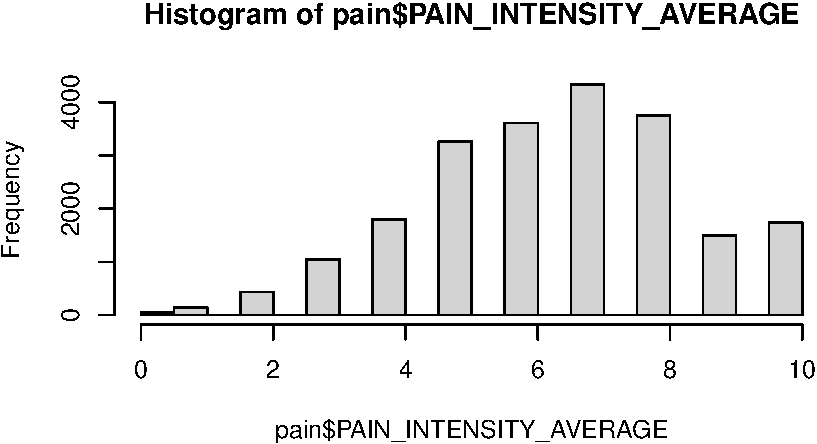
\includegraphics[width=1\textwidth,height=\textheight]{book/working_data_files_files/figure-pdf/unnamed-chunk-12-1.pdf}
\end{center}

\subsection{Practice Question}\label{practice-question-3}

Summarize the \texttt{PROMIS\_SLEEP\_DISTURB\_V1\_0} column both
numerically and visually. Your results should look like the results in
Figure~\ref{fig-sleep-disturb-hist}.

\begin{figure}

\centering{

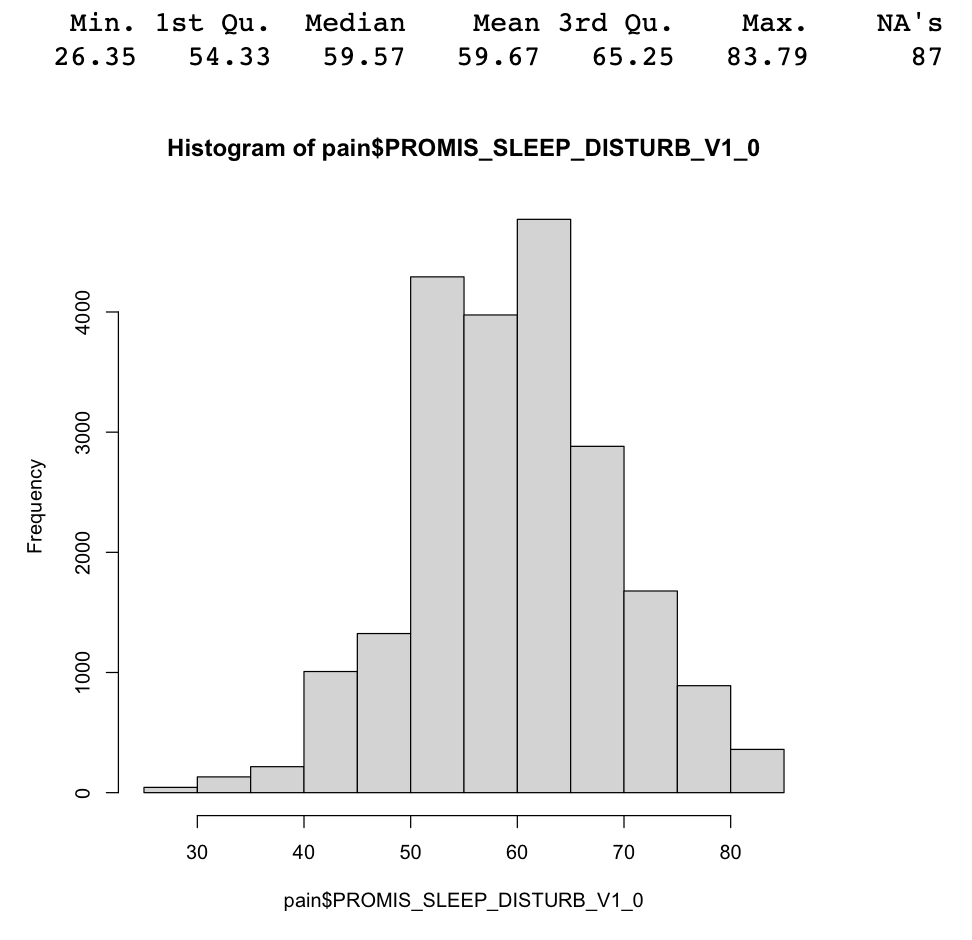
\includegraphics[width=1\textwidth,height=\textheight]{book/images/working_data_files/sleep-disturb-hist.png}

}

\caption{\label{fig-sleep-disturb-hist}Summarizing a Column.}

\end{figure}%

\begin{Shaded}
\begin{Highlighting}[]
\CommentTok{\# Insert your solution here:}
\end{Highlighting}
\end{Shaded}

We can also use the \texttt{summary()} function for categorical
variables. In this case, R finds the counts for each level.

\begin{Shaded}
\begin{Highlighting}[]
\FunctionTok{summary}\NormalTok{(pain}\SpecialCharTok{$}\NormalTok{PAT\_SEX)}
\CommentTok{\#\textgreater{}    Length     Class      Mode }
\CommentTok{\#\textgreater{}     21659 character character}
\end{Highlighting}
\end{Shaded}

For categorical columns, it is also useful to use the
\texttt{table()}\index{R functions!table()@\texttt{table()}} function,
which returns the counts for each possible value, instead of the
\texttt{summary()} function. By default, \texttt{table()} ignores NA
values. However, we can set \texttt{useNA="always"} if we also want to
display the number of NA values in the table output. Additionally, we
can use the
\texttt{prop.table()}\index{R functions!prop.table()@\texttt{prop.table()}}
function to convert the counts to proportions. Using these functions, we
can see that the column \texttt{PAT\_SEX} column, which corresponds to
the reported patient sex, has a single missing value, and we can also
see that around 60\% of patients are female.

\begin{Shaded}
\begin{Highlighting}[]
\FunctionTok{table}\NormalTok{(pain}\SpecialCharTok{$}\NormalTok{PAT\_SEX, }\AttributeTok{useNA=}\StringTok{"always"}\NormalTok{)}
\CommentTok{\#\textgreater{} }
\CommentTok{\#\textgreater{} female   male   \textless{}NA\textgreater{} }
\CommentTok{\#\textgreater{}  13102   8556      1}
\end{Highlighting}
\end{Shaded}

\begin{Shaded}
\begin{Highlighting}[]
\FunctionTok{prop.table}\NormalTok{(}\FunctionTok{table}\NormalTok{(pain}\SpecialCharTok{$}\NormalTok{PAT\_SEX))}
\CommentTok{\#\textgreater{} }
\CommentTok{\#\textgreater{} female   male }
\CommentTok{\#\textgreater{}  0.605  0.395}
\end{Highlighting}
\end{Shaded}

Note that this column is not actually a factor column yet, which we can
check using the \texttt{is.factor()} function. We can convert it to one
using \texttt{as.factor()}.

\begin{Shaded}
\begin{Highlighting}[]
\FunctionTok{is.factor}\NormalTok{(pain}\SpecialCharTok{$}\NormalTok{PAT\_SEX)}
\CommentTok{\#\textgreater{} [1] FALSE}
\end{Highlighting}
\end{Shaded}

\begin{Shaded}
\begin{Highlighting}[]
\NormalTok{pain}\SpecialCharTok{$}\NormalTok{PAT\_SEX }\OtherTok{\textless{}{-}} \FunctionTok{as.factor}\NormalTok{(pain}\SpecialCharTok{$}\NormalTok{PAT\_SEX)}
\FunctionTok{is.factor}\NormalTok{(pain}\SpecialCharTok{$}\NormalTok{PAT\_SEX)}
\CommentTok{\#\textgreater{} [1] TRUE}
\end{Highlighting}
\end{Shaded}

\subsection{Other Summary Functions}\label{other-summary-functions}

Sometimes we want to summarize information across multiple columns or
rows. We can use the
\texttt{rowSums()}\index{R functions!rowSums()@\texttt{rowSums()}} and
\texttt{colSums()}\index{R functions!colSums()@\texttt{colSums()}}
functions to sum over the rows or columns of a matrix or data frame. We
first subset the data to the body pain map regions. In the first line of
code, I select the column names pertaining to these columns. This allows
me to select those columns in the second line of code and store this
subset of the data as a new data frame called \texttt{pain\_body\_map}.

\begin{Shaded}
\begin{Highlighting}[]
\NormalTok{body\_map\_cols }\OtherTok{\textless{}{-}} \FunctionTok{names}\NormalTok{(pain)[}\DecValTok{2}\SpecialCharTok{:}\DecValTok{75}\NormalTok{]}
\NormalTok{pain\_body\_map }\OtherTok{\textless{}{-}}\NormalTok{ pain[, body\_map\_cols]}
\FunctionTok{head}\NormalTok{(pain\_body\_map)}
\CommentTok{\#\textgreater{} \# A tibble: 6 x 74}
\CommentTok{\#\textgreater{}    X101  X102  X103  X104  X105  X106  X107  X108  X109  X110  X111}
\CommentTok{\#\textgreater{}   \textless{}dbl\textgreater{} \textless{}dbl\textgreater{} \textless{}dbl\textgreater{} \textless{}dbl\textgreater{} \textless{}dbl\textgreater{} \textless{}dbl\textgreater{} \textless{}dbl\textgreater{} \textless{}dbl\textgreater{} \textless{}dbl\textgreater{} \textless{}dbl\textgreater{} \textless{}dbl\textgreater{}}
\CommentTok{\#\textgreater{} 1     0     0     0     0     0     0     0     0     0     0     0}
\CommentTok{\#\textgreater{} 2     0     0     0     0     0     0     0     0     0     0     0}
\CommentTok{\#\textgreater{} 3     0     0     0     0     0     0     0     0     0     0     0}
\CommentTok{\#\textgreater{} 4     0     0     0     0     0     0     0     0     0     0     0}
\CommentTok{\#\textgreater{} 5     0     0     0     0     0     0     0     0     0     0     0}
\CommentTok{\#\textgreater{} 6     0     0     0     0     0     0     0     0     0     1     0}
\CommentTok{\#\textgreater{} \# i 63 more variables: X112 \textless{}dbl\textgreater{}, X113 \textless{}dbl\textgreater{}, X114 \textless{}dbl\textgreater{}, X115 \textless{}dbl\textgreater{},}
\CommentTok{\#\textgreater{} \#   X116 \textless{}dbl\textgreater{}, X117 \textless{}dbl\textgreater{}, X118 \textless{}dbl\textgreater{}, X119 \textless{}dbl\textgreater{}, X120 \textless{}dbl\textgreater{},}
\CommentTok{\#\textgreater{} \#   X121 \textless{}dbl\textgreater{}, X122 \textless{}dbl\textgreater{}, X123 \textless{}dbl\textgreater{}, X124 \textless{}dbl\textgreater{}, X125 \textless{}dbl\textgreater{},}
\CommentTok{\#\textgreater{} \#   X126 \textless{}dbl\textgreater{}, X127 \textless{}dbl\textgreater{}, X128 \textless{}dbl\textgreater{}, X129 \textless{}dbl\textgreater{}, X130 \textless{}dbl\textgreater{},}
\CommentTok{\#\textgreater{} \#   X131 \textless{}dbl\textgreater{}, X132 \textless{}dbl\textgreater{}, X133 \textless{}dbl\textgreater{}, X134 \textless{}dbl\textgreater{}, X135 \textless{}dbl\textgreater{},}
\CommentTok{\#\textgreater{} \#   X136 \textless{}dbl\textgreater{}, X201 \textless{}dbl\textgreater{}, X202 \textless{}dbl\textgreater{}, X203 \textless{}dbl\textgreater{}, X204 \textless{}dbl\textgreater{},}
\CommentTok{\#\textgreater{} \#   X205 \textless{}dbl\textgreater{}, X206 \textless{}dbl\textgreater{}, X207 \textless{}dbl\textgreater{}, X208 \textless{}dbl\textgreater{}, X209 \textless{}dbl\textgreater{}, ...}
\end{Highlighting}
\end{Shaded}

I now compute the row sums and column sums on this subset of data. The
row sum for each patient is the total number of body parts in which they
experience pain, whereas the column sum for each pain region is the
total number of patients who experience pain in that area. The following
histogram shows that most people select a low number of total regions.

\begin{Shaded}
\begin{Highlighting}[]
\FunctionTok{hist}\NormalTok{(}\FunctionTok{rowSums}\NormalTok{(pain\_body\_map))}
\end{Highlighting}
\end{Shaded}

\begin{center}
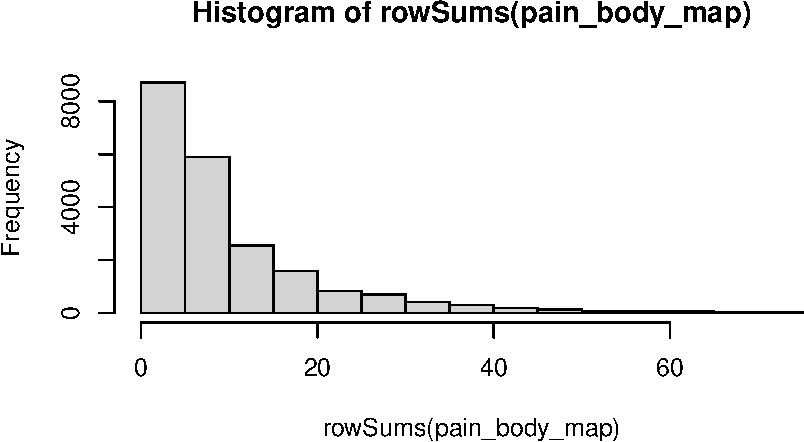
\includegraphics[width=1\textwidth,height=\textheight]{book/working_data_files_files/figure-pdf/unnamed-chunk-20-1.pdf}
\end{center}

We can also see that some body parts are more often selected than
others. We create a vector called \texttt{perc\_patients} by finding the
number of patients who selected each region divided by the total number
of patients. The histogram shows that some body regions are selected by
over 50\% of patients!

\begin{Shaded}
\begin{Highlighting}[]
\NormalTok{perc\_patients }\OtherTok{\textless{}{-}} \FunctionTok{colSums}\NormalTok{(pain\_body\_map, }\AttributeTok{na.rm=}\ConstantTok{TRUE}\NormalTok{) }\SpecialCharTok{/}
  \FunctionTok{nrow}\NormalTok{(pain\_body\_map)}
\FunctionTok{hist}\NormalTok{(perc\_patients)}
\end{Highlighting}
\end{Shaded}

\begin{center}
\includegraphics[width=1\textwidth,height=\textheight]{book/working_data_files_files/figure-pdf/unnamed-chunk-21-1.pdf}
\end{center}

We use the \texttt{which.max()} function to see that the 55th region
\texttt{X219} is selected the most number of times. This corresponds to
lower back pain.

\begin{Shaded}
\begin{Highlighting}[]
\FunctionTok{which.max}\NormalTok{(perc\_patients)}
\CommentTok{\#\textgreater{} X219 }
\CommentTok{\#\textgreater{}   55}
\end{Highlighting}
\end{Shaded}

Another pair of useful functions are
\texttt{pmin()}\index{R functions!pmin()@\texttt{pmin()}} and
\texttt{pmax()}\index{R functions!pmax()@\texttt{pmax()}}. These
functions take at least two vectors and find the pairwise minimum or
maximum across those vectors, as shown in the subsequent code.

\begin{Shaded}
\begin{Highlighting}[]
\NormalTok{v1 }\OtherTok{=} \FunctionTok{c}\NormalTok{(}\DecValTok{5}\NormalTok{, }\DecValTok{9}\NormalTok{, }\DecValTok{12}\NormalTok{)}
\NormalTok{v2 }\OtherTok{=} \FunctionTok{c}\NormalTok{(}\DecValTok{2}\NormalTok{, }\DecValTok{18}\NormalTok{, }\DecValTok{4}\NormalTok{)}
\FunctionTok{pmax}\NormalTok{(v1, v2)  }
\CommentTok{\#\textgreater{} [1]  5 18 12}
\end{Highlighting}
\end{Shaded}

Looking back at the \texttt{pain} data, if we want to create a new
column \texttt{lower\_back\_pain} that corresponds to whether someone
selects \emph{either} X218 or X219 we can use the \texttt{pmax()}
function to find the maximum value between columns \texttt{X218} and
\texttt{X219}. We can see that almost 60\% of patients select at least
one of these regions.

\begin{Shaded}
\begin{Highlighting}[]
\NormalTok{lower\_back }\OtherTok{\textless{}{-}} \FunctionTok{pmax}\NormalTok{(pain\_body\_map}\SpecialCharTok{$}\NormalTok{X218, pain\_body\_map}\SpecialCharTok{$}\NormalTok{X219)}
\FunctionTok{prop.table}\NormalTok{(}\FunctionTok{table}\NormalTok{(lower\_back))}
\CommentTok{\#\textgreater{} lower\_back}
\CommentTok{\#\textgreater{}     0     1 }
\CommentTok{\#\textgreater{} 0.405 0.595}
\end{Highlighting}
\end{Shaded}

We might want to store the total number of pain regions and our
indicator of whether or not a patient has lower back pain as new
columns. We create new columns in the pain data using the \texttt{\$}
operator in the previous code chunk. To be consistent with the column
naming in the data, we use all uppercase for our column names. The
\texttt{dim()} function shows that our data has grown by two columns, as
expected.

\begin{Shaded}
\begin{Highlighting}[]
\NormalTok{pain}\SpecialCharTok{$}\NormalTok{NUM\_REGIONS }\OtherTok{\textless{}{-}} \FunctionTok{rowSums}\NormalTok{(pain\_body\_map)}
\NormalTok{pain}\SpecialCharTok{$}\NormalTok{LOWER\_BACK }\OtherTok{\textless{}{-}}\NormalTok{ lower\_back}
\FunctionTok{dim}\NormalTok{(pain)}
\CommentTok{\#\textgreater{} [1] 21659    94}
\end{Highlighting}
\end{Shaded}

Another useful function that allows us to perform computations over the
rows or columns of a matrix or data frame is the
\texttt{apply(X,\ MARGIN,\ FUN)}
function\index{R functions!apply()@\texttt{apply()}}, which takes in
three arguments. The first argument is a data frame or matrix
\texttt{X}, the second argument \texttt{MARGIN} indicates whether to
compute over the rows (\texttt{1}) or columns (\texttt{2}), and the last
argument is the function \texttt{FUN} to apply across that margin. The
subsequent code finds the maximum value for each row in the data frame
\texttt{pain\_body\_map}. Taking the minimum value of the row maximum
values shows that every patient selected at least one body map region.

\begin{Shaded}
\begin{Highlighting}[]
\NormalTok{any\_selected }\OtherTok{\textless{}{-}} \FunctionTok{apply}\NormalTok{(pain\_body\_map, }\DecValTok{1}\NormalTok{, max)}
\FunctionTok{min}\NormalTok{(any\_selected, }\AttributeTok{na.rm=}\ConstantTok{TRUE}\NormalTok{)}
\CommentTok{\#\textgreater{} [1] 1}
\end{Highlighting}
\end{Shaded}

In a second example, we find the sum of the body pain regions over the
columns, which is equivalent to the previous example using
\texttt{colSums()}. In this case, we added the \texttt{na.rm=TRUE}
argument. The \texttt{apply()} function passes any additional arguments
to the function \texttt{FUN}.

\begin{Shaded}
\begin{Highlighting}[]
\NormalTok{perc\_patients }\OtherTok{\textless{}{-}} \FunctionTok{apply}\NormalTok{(pain\_body\_map, }\DecValTok{2}\NormalTok{, sum, }\AttributeTok{na.rm=}\ConstantTok{TRUE}\NormalTok{) }\SpecialCharTok{/}
  \FunctionTok{nrow}\NormalTok{(pain\_body\_map)}
\FunctionTok{summary}\NormalTok{(perc\_patients)}
\CommentTok{\#\textgreater{}    Min. 1st Qu.  Median    Mean 3rd Qu.    Max. }
\CommentTok{\#\textgreater{}   0.032   0.070   0.136   0.144   0.181   0.542}
\end{Highlighting}
\end{Shaded}

\subsection{Practice Question}\label{practice-question-4}

Find the sum of each of the PROMIS measures across all patients using
\texttt{apply()} and then using \texttt{colSums()}. Verify that these
two methods return the same result, which is given in
Figure~\ref{fig-promis-col-sums}.

\begin{figure}

\centering{

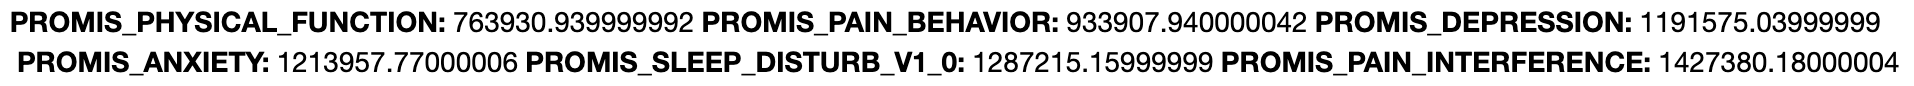
\includegraphics[width=1\textwidth,height=\textheight]{book/images/working_data_files/promis-col-sums.png}

}

\caption{\label{fig-promis-col-sums}Summing Across Columns.}

\end{figure}%

\begin{Shaded}
\begin{Highlighting}[]
\CommentTok{\# Insert your solution here:}
\end{Highlighting}
\end{Shaded}

\subsection{\texorpdfstring{Missing, Infinite, and NaN Values
\index{missing values} \index{NA values} \index{infinite values}
\index{NaN values}}{Missing, Infinite, and NaN Values    }}\label{missing-infinite-and-nan-values}

As we have seen, this data contains some missing values, which are
represented as \texttt{NA} in R. R treats these values as if they were
unknown, which is why we have to add the \texttt{na.rm=TRUE} argument to
functions like \texttt{sum()} and \texttt{max()}. In the following
example, we can see that R figures out that 1 plus an unknown number is
also unknown!

\begin{Shaded}
\begin{Highlighting}[]
\ConstantTok{NA}\SpecialCharTok{+}\DecValTok{1}
\CommentTok{\#\textgreater{} [1] NA}
\end{Highlighting}
\end{Shaded}

We can determine whether a value is missing using the function
\texttt{is.na()}\index{R functions!is.na()@\texttt{is.na()}}. This
function returns \texttt{TRUE} if the value is NA, and \texttt{FALSE}
otherwise. We can then sum up these values for a single column since
each \texttt{TRUE} value corresponds to a value of 1, and each
\texttt{FALSE} corresponds to a value of 0. We observe that there is a
single NA value for the column \texttt{PATIENT\_NUM}, which is the
patient ID number.

\begin{Shaded}
\begin{Highlighting}[]
\FunctionTok{sum}\NormalTok{(}\FunctionTok{is.na}\NormalTok{(pain}\SpecialCharTok{$}\NormalTok{PATIENT\_NUM))}
\CommentTok{\#\textgreater{} [1] 1}
\end{Highlighting}
\end{Shaded}

If we want to calculate the sum of NA values for each column instead of
just a single column, we can use the \texttt{apply()} function. Since we
want to apply this computation over the columns, the second argument has
value 2. Recall that the last argument is the function we want to call
for each column. In this case, we want to apply the combination of the
\texttt{sum()} and \texttt{is.na()} function. To do so, we have to
specify this function ourselves. This is called an \textbf{anonymous
function} \index{anonymous function}, since it doesn't have a name.

\begin{Shaded}
\begin{Highlighting}[]
\NormalTok{num\_missing\_col }\OtherTok{\textless{}{-}} \FunctionTok{apply}\NormalTok{(pain, }\DecValTok{2}\NormalTok{, }\ControlFlowTok{function}\NormalTok{(x) }\FunctionTok{sum}\NormalTok{(}\FunctionTok{is.na}\NormalTok{(x)))}
\FunctionTok{min}\NormalTok{(num\_missing\_col)}
\CommentTok{\#\textgreater{} [1] 1}
\end{Highlighting}
\end{Shaded}

Interestingly, we can see that there is at least one missing value in
each column. It might be the case that there is a row with all NA
values. Let's apply the same function by row. Taking the maximum, we can
see that row 11749 has all NA values.

\begin{Shaded}
\begin{Highlighting}[]
\NormalTok{num\_missing\_row }\OtherTok{\textless{}{-}} \FunctionTok{apply}\NormalTok{(pain, }\DecValTok{1}\NormalTok{, }\ControlFlowTok{function}\NormalTok{(x) }\FunctionTok{sum}\NormalTok{(}\FunctionTok{is.na}\NormalTok{(x)))}
\FunctionTok{max}\NormalTok{(num\_missing\_row)}
\CommentTok{\#\textgreater{} [1] 94}
\FunctionTok{which.max}\NormalTok{(num\_missing\_row)}
\CommentTok{\#\textgreater{} [1] 11749}
\end{Highlighting}
\end{Shaded}

We remove that row and then find the percentage of missing values by
column. We can see that the column with the highest percentage of
missing values is the pain intensity at follow-up. In fact, only 33\% of
patients have a recorded follow-up visit.

\begin{Shaded}
\begin{Highlighting}[]
\NormalTok{pain }\OtherTok{\textless{}{-}}\NormalTok{ pain[}\SpecialCharTok{{-}}\DecValTok{11749}\NormalTok{, ]}
\NormalTok{num\_missing\_col }\OtherTok{\textless{}{-}} \FunctionTok{apply}\NormalTok{(pain, }\DecValTok{2}\NormalTok{, }
                         \ControlFlowTok{function}\NormalTok{(x) }\FunctionTok{sum}\NormalTok{(}\FunctionTok{is.na}\NormalTok{(x))}\SpecialCharTok{/}\FunctionTok{nrow}\NormalTok{(pain))}
\NormalTok{num\_missing\_col}
\CommentTok{\#\textgreater{}                      PATIENT\_NUM                             X101 }
\CommentTok{\#\textgreater{}                          0.00000                          0.00000 }
\CommentTok{\#\textgreater{}                             X102                             X103 }
\CommentTok{\#\textgreater{}                          0.00000                          0.00000 }
\CommentTok{\#\textgreater{}                             X104                             X105 }
\CommentTok{\#\textgreater{}                          0.00000                          0.00000 }
\CommentTok{\#\textgreater{}                             X106                             X107 }
\CommentTok{\#\textgreater{}                          0.00000                          0.00000 }
\CommentTok{\#\textgreater{}                             X108                             X109 }
\CommentTok{\#\textgreater{}                          0.00000                          0.00000 }
\CommentTok{\#\textgreater{}                             X110                             X111 }
\CommentTok{\#\textgreater{}                          0.00000                          0.00000 }
\CommentTok{\#\textgreater{}                             X112                             X113 }
\CommentTok{\#\textgreater{}                          0.00000                          0.00000 }
\CommentTok{\#\textgreater{}                             X114                             X115 }
\CommentTok{\#\textgreater{}                          0.00000                          0.00000 }
\CommentTok{\#\textgreater{}                             X116                             X117 }
\CommentTok{\#\textgreater{}                          0.00000                          0.00000 }
\CommentTok{\#\textgreater{}                             X118                             X119 }
\CommentTok{\#\textgreater{}                          0.00000                          0.00000 }
\CommentTok{\#\textgreater{}                             X120                             X121 }
\CommentTok{\#\textgreater{}                          0.00000                          0.00000 }
\CommentTok{\#\textgreater{}                             X122                             X123 }
\CommentTok{\#\textgreater{}                          0.00000                          0.00000 }
\CommentTok{\#\textgreater{}                             X124                             X125 }
\CommentTok{\#\textgreater{}                          0.00000                          0.00000 }
\CommentTok{\#\textgreater{}                             X126                             X127 }
\CommentTok{\#\textgreater{}                          0.00000                          0.00000 }
\CommentTok{\#\textgreater{}                             X128                             X129 }
\CommentTok{\#\textgreater{}                          0.00000                          0.00000 }
\CommentTok{\#\textgreater{}                             X130                             X131 }
\CommentTok{\#\textgreater{}                          0.00000                          0.00000 }
\CommentTok{\#\textgreater{}                             X132                             X133 }
\CommentTok{\#\textgreater{}                          0.00000                          0.00000 }
\CommentTok{\#\textgreater{}                             X134                             X135 }
\CommentTok{\#\textgreater{}                          0.00000                          0.00000 }
\CommentTok{\#\textgreater{}                             X136                             X201 }
\CommentTok{\#\textgreater{}                          0.00000                          0.00000 }
\CommentTok{\#\textgreater{}                             X202                             X203 }
\CommentTok{\#\textgreater{}                          0.00000                          0.00000 }
\CommentTok{\#\textgreater{}                             X204                             X205 }
\CommentTok{\#\textgreater{}                          0.00000                          0.00000 }
\CommentTok{\#\textgreater{}                             X206                             X207 }
\CommentTok{\#\textgreater{}                          0.00000                          0.00000 }
\CommentTok{\#\textgreater{}                             X208                             X209 }
\CommentTok{\#\textgreater{}                          0.00000                          0.00000 }
\CommentTok{\#\textgreater{}                             X210                             X211 }
\CommentTok{\#\textgreater{}                          0.00000                          0.00000 }
\CommentTok{\#\textgreater{}                             X212                             X213 }
\CommentTok{\#\textgreater{}                          0.00000                          0.00000 }
\CommentTok{\#\textgreater{}                             X214                             X215 }
\CommentTok{\#\textgreater{}                          0.00000                          0.00000 }
\CommentTok{\#\textgreater{}                             X216                             X217 }
\CommentTok{\#\textgreater{}                          0.00000                          0.00000 }
\CommentTok{\#\textgreater{}                             X218                             X219 }
\CommentTok{\#\textgreater{}                          0.00000                          0.00000 }
\CommentTok{\#\textgreater{}                             X220                             X221 }
\CommentTok{\#\textgreater{}                          0.00000                          0.00000 }
\CommentTok{\#\textgreater{}                             X222                             X223 }
\CommentTok{\#\textgreater{}                          0.00000                          0.00000 }
\CommentTok{\#\textgreater{}                             X224                             X225 }
\CommentTok{\#\textgreater{}                          0.00000                          0.00000 }
\CommentTok{\#\textgreater{}                             X226                             X227 }
\CommentTok{\#\textgreater{}                          0.00000                          0.00000 }
\CommentTok{\#\textgreater{}                             X228                             X229 }
\CommentTok{\#\textgreater{}                          0.00000                          0.00000 }
\CommentTok{\#\textgreater{}                             X230                             X231 }
\CommentTok{\#\textgreater{}                          0.00000                          0.00000 }
\CommentTok{\#\textgreater{}                             X232                             X233 }
\CommentTok{\#\textgreater{}                          0.00000                          0.00000 }
\CommentTok{\#\textgreater{}                             X234                             X235 }
\CommentTok{\#\textgreater{}                          0.00000                          0.00000 }
\CommentTok{\#\textgreater{}                             X236                             X237 }
\CommentTok{\#\textgreater{}                          0.00000                          0.00000 }
\CommentTok{\#\textgreater{}                             X238           PAIN\_INTENSITY\_AVERAGE }
\CommentTok{\#\textgreater{}                          0.00000                          0.00000 }
\CommentTok{\#\textgreater{}         PROMIS\_PHYSICAL\_FUNCTION             PROMIS\_PAIN\_BEHAVIOR }
\CommentTok{\#\textgreater{}                          0.00000                          0.29412 }
\CommentTok{\#\textgreater{}                PROMIS\_DEPRESSION                   PROMIS\_ANXIETY }
\CommentTok{\#\textgreater{}                          0.00402                          0.00402 }
\CommentTok{\#\textgreater{}        PROMIS\_SLEEP\_DISTURB\_V1\_0         PROMIS\_PAIN\_INTERFERENCE }
\CommentTok{\#\textgreater{}                          0.00402                          0.00697 }
\CommentTok{\#\textgreater{}                  GH\_MENTAL\_SCORE                GH\_PHYSICAL\_SCORE }
\CommentTok{\#\textgreater{}                          0.13602                          0.13602 }
\CommentTok{\#\textgreater{}                   AGE\_AT\_CONTACT                              BMI }
\CommentTok{\#\textgreater{}                          0.00000                          0.26004 }
\CommentTok{\#\textgreater{}                  CCI\_TOTAL\_SCORE PAIN\_INTENSITY\_AVERAGE.FOLLOW\_UP }
\CommentTok{\#\textgreater{}                          0.00000                          0.67042 }
\CommentTok{\#\textgreater{}                          PAT\_SEX                         PAT\_RACE }
\CommentTok{\#\textgreater{}                          0.00000                          0.00651 }
\CommentTok{\#\textgreater{}                          CCI\_BIN                     MEDICAID\_BIN }
\CommentTok{\#\textgreater{}                          0.00000                          0.01385 }
\CommentTok{\#\textgreater{}                      NUM\_REGIONS                       LOWER\_BACK }
\CommentTok{\#\textgreater{}                          0.00000                          0.00000}
\end{Highlighting}
\end{Shaded}

We create two new columns: first, we create a column for the change in
pain at follow-up, and second, we create a column for the percent change
in pain at follow-up.

\begin{Shaded}
\begin{Highlighting}[]
\NormalTok{pain}\SpecialCharTok{$}\NormalTok{PAIN\_CHANGE }\OtherTok{\textless{}{-}}\NormalTok{ pain}\SpecialCharTok{$}\NormalTok{PAIN\_INTENSITY\_AVERAGE.FOLLOW\_UP }\SpecialCharTok{{-}} 
\NormalTok{  pain}\SpecialCharTok{$}\NormalTok{PAIN\_INTENSITY\_AVERAGE}
\FunctionTok{hist}\NormalTok{(pain}\SpecialCharTok{$}\NormalTok{PAIN\_CHANGE)}
\end{Highlighting}
\end{Shaded}

\begin{center}
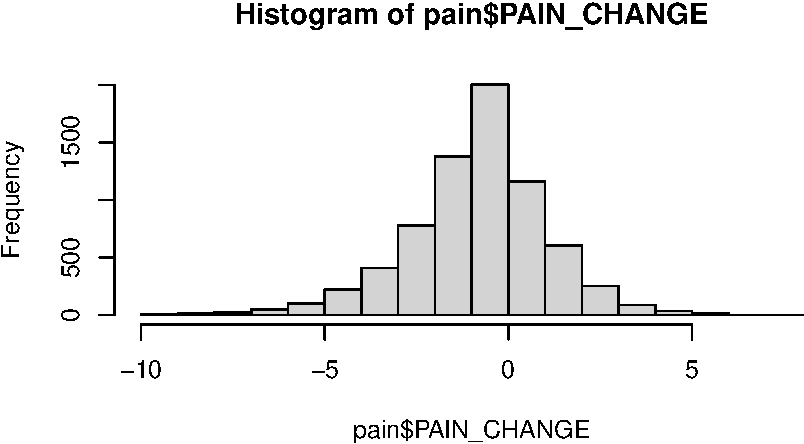
\includegraphics[width=1\textwidth,height=\textheight]{book/working_data_files_files/figure-pdf/unnamed-chunk-34-1.pdf}
\end{center}

\begin{Shaded}
\begin{Highlighting}[]
\NormalTok{pain}\SpecialCharTok{$}\NormalTok{PERC\_PAIN\_CHANGE }\OtherTok{\textless{}{-}}\NormalTok{ pain}\SpecialCharTok{$}\NormalTok{PAIN\_CHANGE }\SpecialCharTok{/} 
\NormalTok{  pain}\SpecialCharTok{$}\NormalTok{PAIN\_INTENSITY\_AVERAGE}
\FunctionTok{summary}\NormalTok{(pain}\SpecialCharTok{$}\NormalTok{PERC\_PAIN\_CHANGE)}
\CommentTok{\#\textgreater{}    Min. 1st Qu.  Median    Mean 3rd Qu.    Max.    NA\textquotesingle{}s }
\CommentTok{\#\textgreater{}      {-}1       0       0     Inf       0     Inf   14520}
\end{Highlighting}
\end{Shaded}

In the summary of the percent change, we can see that the maximum value
is \texttt{Inf}. This is R's representation of infinity. This occurred
because some patients have an initial pain score of 0, which creates
infinite values when we divide through by this value to find the percent
change. We can test whether something is infinite using the
\texttt{is.infinite()}\index{R functions!is.infinite()@\texttt{is.infinite()}}
or
\texttt{is.finite()}\index{R functions!is.finite()@\texttt{is.finite()}}
functions. This shows that there were three patients with infinite
values. The value \texttt{-Inf} is used to represent negative infinity.

\begin{Shaded}
\begin{Highlighting}[]
\FunctionTok{sum}\NormalTok{(}\FunctionTok{is.infinite}\NormalTok{(pain}\SpecialCharTok{$}\NormalTok{PERC\_PAIN\_CHANGE))}
\CommentTok{\#\textgreater{} [1] 3}
\end{Highlighting}
\end{Shaded}

Another special value in R is \texttt{NaN}, which stands for ``Not a
Number''. For example, \texttt{0/0} results in a NaN value. We can test
for \texttt{NaN} values using the \texttt{is.nan()} function.

\begin{Shaded}
\begin{Highlighting}[]
\DecValTok{0}\SpecialCharTok{/}\DecValTok{0}
\CommentTok{\#\textgreater{} [1] NaN}
\end{Highlighting}
\end{Shaded}

Looking back at the missing values, there are two useful functions for
selecting the complete cases in a data frame. The
\texttt{na.omit()}\index{R functions!na.omit()@\texttt{na.omit()}}
function returns the data frame with incomplete cases removed, whereas
\texttt{complete.cases()}\index{R functions!complete.cases()@\texttt{complete.cases()}}
returns TRUE/FALSE values for each row indicating whether each row is
complete, which we can then use to select the rows with TRUE values. In
the following code, we see that both approaches select the same number
of rows.

\begin{Shaded}
\begin{Highlighting}[]
\NormalTok{pain\_sub1 }\OtherTok{\textless{}{-}} \FunctionTok{na.omit}\NormalTok{(pain)}
\NormalTok{pain\_sub2 }\OtherTok{\textless{}{-}}\NormalTok{ pain[}\FunctionTok{complete.cases}\NormalTok{(pain), ]}
\FunctionTok{dim}\NormalTok{(pain\_sub1)}
\CommentTok{\#\textgreater{} [1] 2413   96}
\FunctionTok{dim}\NormalTok{(pain\_sub2)}
\CommentTok{\#\textgreater{} [1] 2413   96}
\end{Highlighting}
\end{Shaded}

\subsection{\texorpdfstring{Dates in R
\index{dates}}{Dates in R }}\label{dates-in-r}

The columns in the \texttt{pain} data contain character and numeric
values. One special type of character column that is not present is a
column that corresponds to a date or date-time. By default,
\texttt{read.csv()} reads these columns in as character columns, whereas
the \texttt{read\_csv()} function from the
\textbf{readr}\index{R packages!readr} package in the \textbf{tidyverse}
family recognizes common date formats. If we have a character column, we
can convert to a date object using
\texttt{as.Date()}\index{R functions!as.Date()@\texttt{as.Date()}} for
date columns and
\texttt{as.POSIXct()}\index{R functions!as.POSIXct()@\texttt{as.POSIXct()}}
for date-time columns. For columns with only a time but no date, you can
add a date or use the \textbf{hms}\index{R packages!hms} package (Müller
2023), which is not demonstrated here. These functions automatically try
to detect the format of the inputted string, but it is often helpful to
provide the \texttt{format} and time zone \texttt{tz}. To input our
format we use the following key\index{date format}.

\begin{longtable}[]{@{}ll@{}}
\toprule\noalign{}
Symbol & Description \\
\midrule\noalign{}
\endhead
\bottomrule\noalign{}
\endlastfoot
\%Y & Four-digit year. \\
\%y & Two-digit year. \\
\%m & Numeric month. \\
\%b\% & Abbreviated name of month. \\
\%B & Full name of month. \\
\%d & Numeric day of the month. \\
\%H & Military time hour (24 hours). \\
\%I & Imperial time hour (12 hours). \\
\%M & Minute. \\
\%S & Seconds. \\
\%p & AM/PM \\
\end{longtable}

\begin{Shaded}
\begin{Highlighting}[]
\NormalTok{date\_example }\OtherTok{\textless{}{-}} \FunctionTok{data.frame}\NormalTok{(}\AttributeTok{x =} \FunctionTok{c}\NormalTok{(}\StringTok{"2020{-}01{-}15"}\NormalTok{, }\StringTok{"2021{-}11{-}16"}\NormalTok{, }
                                 \StringTok{"2019{-}08{-}01"}\NormalTok{),}
                           \AttributeTok{y =} \FunctionTok{c}\NormalTok{(}\StringTok{"2020{-}01{-}15 3:14 PM"}\NormalTok{, }
                                 \StringTok{"2021{-}11{-}16 5:00 AM"}\NormalTok{,}
                                 \StringTok{"2019{-}08{-}01 3:00 PM"}\NormalTok{),}
                           \AttributeTok{z =} \FunctionTok{c}\NormalTok{(}\StringTok{"04:10:00"}\NormalTok{, }\StringTok{"11:35:11"}\NormalTok{, }\StringTok{"18:00:45"}\NormalTok{))}

\CommentTok{\# Convert date and date times using formats}
\NormalTok{date\_example}\SpecialCharTok{$}\NormalTok{x }\OtherTok{\textless{}{-}} \FunctionTok{as.Date}\NormalTok{(date\_example}\SpecialCharTok{$}\NormalTok{x, }\AttributeTok{format =} \StringTok{"\%Y{-}\%m{-}\%d"}\NormalTok{, }
                          \AttributeTok{tz =} \StringTok{"EST"}\NormalTok{)}
\NormalTok{date\_example}\SpecialCharTok{$}\NormalTok{y }\OtherTok{\textless{}{-}} \FunctionTok{as.POSIXct}\NormalTok{(date\_example}\SpecialCharTok{$}\NormalTok{y, }
                             \AttributeTok{format =} \StringTok{"\%Y{-}\%m{-}\%d \%I:\%M \%p"}\NormalTok{)}

\CommentTok{\# Add date to z and convert}
\NormalTok{date\_example}\SpecialCharTok{$}\NormalTok{z }\OtherTok{\textless{}{-}} \FunctionTok{paste}\NormalTok{(}\StringTok{"2024{-}06{-}24"}\NormalTok{, date\_example}\SpecialCharTok{$}\NormalTok{z)}
\NormalTok{date\_example}\SpecialCharTok{$}\NormalTok{z }\OtherTok{\textless{}{-}} \FunctionTok{as.POSIXct}\NormalTok{(date\_example}\SpecialCharTok{$}\NormalTok{z, }
                             \AttributeTok{format =} \StringTok{"\%Y{-}\%m{-}\%d \%H:\%M:\%S"}\NormalTok{)}
\NormalTok{date\_example}
\CommentTok{\#\textgreater{}            x                   y                   z}
\CommentTok{\#\textgreater{} 1 2020{-}01{-}15 2020{-}01{-}15 15:14:00 2024{-}06{-}24 04:10:00}
\CommentTok{\#\textgreater{} 2 2021{-}11{-}16 2021{-}11{-}16 05:00:00 2024{-}06{-}24 11:35:11}
\CommentTok{\#\textgreater{} 3 2019{-}08{-}01 2019{-}08{-}01 15:00:00 2024{-}06{-}24 18:00:45}
\end{Highlighting}
\end{Shaded}

By recognizing these columns as dates, we can find the time between two
dates using the
\texttt{difftime()}\index{R functions!difftime()@\texttt{difftime()}}
function. This function takes in two times \texttt{time1} and
\texttt{time2} and finds the difference \texttt{time1\ -\ time2} in the
given \texttt{units}.

\begin{Shaded}
\begin{Highlighting}[]
\FunctionTok{difftime}\NormalTok{(date\_example}\SpecialCharTok{$}\NormalTok{x[}\DecValTok{2}\NormalTok{], date\_example}\SpecialCharTok{$}\NormalTok{x[}\DecValTok{1}\NormalTok{], }\AttributeTok{units =} \StringTok{"days"}\NormalTok{)}
\CommentTok{\#\textgreater{} Time difference of 671 days}
\end{Highlighting}
\end{Shaded}

Additionally, we can use the \texttt{seq()} function to add or subtract
time by specifying a unit for \texttt{by}.

\begin{Shaded}
\begin{Highlighting}[]
\FunctionTok{seq}\NormalTok{(date\_example}\SpecialCharTok{$}\NormalTok{x[}\DecValTok{1}\NormalTok{], }\AttributeTok{by =} \StringTok{"month"}\NormalTok{, }\AttributeTok{length =} \DecValTok{3}\NormalTok{)}
\CommentTok{\#\textgreater{} [1] "2020{-}01{-}15" "2020{-}02{-}15" "2020{-}03{-}15"}
\end{Highlighting}
\end{Shaded}

For those interested in doing more manipulations with dates, the
\textbf{lubridate} package\index{R packages!lubridate} (Spinu,
Grolemund, and Wickham 2023) in the \textbf{tidyverse} expands upon the
base functionality of R for working with dates. This package uses its
own date-time class and includes functions to easily extract information
from and manipulate dates.

\section{\texorpdfstring{Using Logic to Subset, Summarize, and Transform
\index{subset data}}{Using Logic to Subset, Summarize, and Transform }}\label{using-logic-to-subset-summarize-and-transform}

We have already seen how to use TRUE/FALSE values to select rows in a
data frame. The following logic operators in R allow us to expand on
this capability to write more complex logic\index{logical operators}.

\begin{itemize}
\tightlist
\item
  \texttt{\textless{}} less than
\item
  \texttt{\textless{}=} less than or equal to
\item
  \texttt{\textgreater{}} greater than
\item
  \texttt{\textgreater{}=} greater than or equal to
\item
  \texttt{==} equal to
\item
  \texttt{!=} not equal to
\item
  \texttt{a\ \%in\%\ b} a's value is in a vector of values b
\end{itemize}

The first six operators are a direct comparison between two values.

\begin{Shaded}
\begin{Highlighting}[]
\DecValTok{2} \SpecialCharTok{\textless{}} \DecValTok{2}
\CommentTok{\#\textgreater{} [1] FALSE}
\DecValTok{2} \SpecialCharTok{\textless{}=} \DecValTok{2}
\CommentTok{\#\textgreater{} [1] TRUE}
\DecValTok{3} \SpecialCharTok{\textgreater{}} \DecValTok{2}
\CommentTok{\#\textgreater{} [1] TRUE}
\DecValTok{3} \SpecialCharTok{\textgreater{}=} \DecValTok{2}
\CommentTok{\#\textgreater{} [1] TRUE}
\StringTok{"A"} \SpecialCharTok{==} \StringTok{"B"}
\CommentTok{\#\textgreater{} [1] FALSE}
\StringTok{"A"} \SpecialCharTok{!=} \StringTok{"B"}
\CommentTok{\#\textgreater{} [1] TRUE}
\end{Highlighting}
\end{Shaded}

The operators assume there is a natural ordering or comparison between
values. For example, for strings the ordering is alphabetical and for
logical operators we use their numeric interpretation (TRUE = 1, FALSE =
0).

\begin{Shaded}
\begin{Highlighting}[]
\StringTok{"A"} \SpecialCharTok{\textless{}} \StringTok{"B"}
\CommentTok{\#\textgreater{} [1] TRUE}
\ConstantTok{TRUE} \SpecialCharTok{\textless{}} \ConstantTok{FALSE}
\CommentTok{\#\textgreater{} [1] FALSE}
\end{Highlighting}
\end{Shaded}

The \texttt{\%in\%} operator is slightly different. This operator checks
whether a value is in a set of possible values. For example, we can
check whether values are in the set \texttt{c(4,1,2)}.

\begin{Shaded}
\begin{Highlighting}[]
\DecValTok{1} \SpecialCharTok{\%in\%} \FunctionTok{c}\NormalTok{(}\DecValTok{4}\NormalTok{, }\DecValTok{1}\NormalTok{, }\DecValTok{2}\NormalTok{)}
\CommentTok{\#\textgreater{} [1] TRUE}
\FunctionTok{c}\NormalTok{(}\DecValTok{0}\NormalTok{, }\DecValTok{1}\NormalTok{, }\DecValTok{5}\NormalTok{) }\SpecialCharTok{\%in\%} \FunctionTok{c}\NormalTok{(}\DecValTok{4}\NormalTok{, }\DecValTok{1}\NormalTok{, }\DecValTok{2}\NormalTok{)}
\CommentTok{\#\textgreater{} [1] FALSE  TRUE FALSE}
\end{Highlighting}
\end{Shaded}

Additionally, we can use the following operators, which allow us to
negate or combine logical operators\index{logical operators}.

\begin{itemize}
\tightlist
\item
  \texttt{!x} - the \textbf{NOT} operator \texttt{!} reverses TRUE/FALSE
  values
\item
  \texttt{x\ \textbar{}\ y} - the \textbf{OR} operator
  \texttt{\textbar{}} checks whether \emph{either} x or y is equal to
  TRUE
\item
  \texttt{x\ \&\ y} - the \textbf{AND} operator \texttt{\&} checks
  whether \emph{both} x and y are equal to TRUE
\item
  \texttt{xor(x,y)} - the \textbf{xor} function checks whether exactly
  one of x or y is equal to TRUE (called exclusive or)
  \index{R functions!xor()@\texttt{xor()}}
\item
  \texttt{any(x)} - the \textbf{any} function checks whether any value
  in x is TRUE (equivalent to using an OR operator \texttt{\textbar{}}
  between all values) \index{R functions!any()@\texttt{any()}}
\item
  \texttt{all(x)} - the \textbf{all} function checks whether all values
  in x are TRUE (equivalent to using an AND operator \texttt{\&} between
  all values) \index{R functions!all()@\texttt{all()}}
\end{itemize}

Some simple examples for each are given in the following code chunk.

\begin{Shaded}
\begin{Highlighting}[]
\SpecialCharTok{!}\NormalTok{(}\DecValTok{2} \SpecialCharTok{\textless{}} \DecValTok{3}\NormalTok{)}
\CommentTok{\#\textgreater{} [1] FALSE}
\NormalTok{(}\StringTok{"Alice"} \SpecialCharTok{\textless{}} \StringTok{"Bob"}\NormalTok{) }\SpecialCharTok{|}\NormalTok{ (}\StringTok{"Alice"} \SpecialCharTok{\textless{}} \StringTok{"Aaron"}\NormalTok{)}
\CommentTok{\#\textgreater{} [1] TRUE}
\NormalTok{(}\StringTok{"Alice"} \SpecialCharTok{\textless{}} \StringTok{"Bob"}\NormalTok{) }\SpecialCharTok{\&}\NormalTok{ (}\StringTok{"Alice"} \SpecialCharTok{\textless{}} \StringTok{"Aaron"}\NormalTok{)}
\CommentTok{\#\textgreater{} [1] FALSE}
\FunctionTok{xor}\NormalTok{(}\ConstantTok{TRUE}\NormalTok{, }\ConstantTok{FALSE}\NormalTok{)}
\CommentTok{\#\textgreater{} [1] TRUE}
\FunctionTok{any}\NormalTok{(}\FunctionTok{c}\NormalTok{(}\ConstantTok{FALSE}\NormalTok{, }\ConstantTok{TRUE}\NormalTok{, }\ConstantTok{TRUE}\NormalTok{))}
\CommentTok{\#\textgreater{} [1] TRUE}
\FunctionTok{all}\NormalTok{(}\FunctionTok{c}\NormalTok{(}\ConstantTok{FALSE}\NormalTok{, }\ConstantTok{TRUE}\NormalTok{, }\ConstantTok{TRUE}\NormalTok{))}
\CommentTok{\#\textgreater{} [1] FALSE}
\end{Highlighting}
\end{Shaded}

Let's demonstrate these operators on the pain data. We first update the
Medicaid column by making the character values more informative. The
logic on the left-hand side selects those who do or do not have Medicaid
and then assigns those values to the new ones.

\begin{Shaded}
\begin{Highlighting}[]
\NormalTok{pain}\SpecialCharTok{$}\NormalTok{MEDICAID\_BIN[pain}\SpecialCharTok{$}\NormalTok{MEDICAID\_BIN }\SpecialCharTok{==} \StringTok{"no"}\NormalTok{] }\OtherTok{\textless{}{-}} \StringTok{"No Medicaid"}
\NormalTok{pain}\SpecialCharTok{$}\NormalTok{MEDICAID\_BIN[pain}\SpecialCharTok{$}\NormalTok{MEDICAID\_BIN }\SpecialCharTok{==} \StringTok{"yes"}\NormalTok{] }\OtherTok{\textless{}{-}} \StringTok{"Medicaid"}
\FunctionTok{table}\NormalTok{(pain}\SpecialCharTok{$}\NormalTok{MEDICAID\_BIN)}
\CommentTok{\#\textgreater{} }
\CommentTok{\#\textgreater{}    Medicaid No Medicaid }
\CommentTok{\#\textgreater{}        4601       16757}
\end{Highlighting}
\end{Shaded}

Additionally, we could subset the data to only those who have a
follow-up. The not operator \texttt{!} reverses the TRUE/FALSE values
returned from the \texttt{is.na()} function. Therefore, the new value is
TRUE if the follow-up value is \emph{not} NA.

\begin{Shaded}
\begin{Highlighting}[]
\NormalTok{pain\_follow\_up }\OtherTok{\textless{}{-}}\NormalTok{ pain[}\SpecialCharTok{!}\FunctionTok{is.na}\NormalTok{(pain}\SpecialCharTok{$}\NormalTok{PAIN\_INTENSITY\_AVERAGE.FOLLOW\_UP), ]}
\end{Highlighting}
\end{Shaded}

Earlier, we created a column indicating whether or not a patient has
lower back pain. We now use the \texttt{\textbar{}} operator and the
\texttt{pmax()} function to check whether a patient has general back
pain. If at least one of the back region areas has value 1, then either
of these approaches will return \texttt{TRUE}.

\begin{Shaded}
\begin{Highlighting}[]
\NormalTok{pain}\SpecialCharTok{$}\NormalTok{BACK }\OtherTok{\textless{}{-}} \FunctionTok{pmax}\NormalTok{(pain}\SpecialCharTok{$}\NormalTok{X208, pain}\SpecialCharTok{$}\NormalTok{X209, pain}\SpecialCharTok{$}\NormalTok{X212, }
\NormalTok{                 pain}\SpecialCharTok{$}\NormalTok{X213, pain}\SpecialCharTok{$}\NormalTok{X218, pain}\SpecialCharTok{$}\NormalTok{X219) }\SpecialCharTok{==} \DecValTok{1}
\NormalTok{pain}\SpecialCharTok{$}\NormalTok{BACK }\OtherTok{\textless{}{-}}\NormalTok{ (pain}\SpecialCharTok{$}\NormalTok{X208}\SpecialCharTok{==}\DecValTok{1}\NormalTok{) }\SpecialCharTok{|}\NormalTok{ (pain}\SpecialCharTok{$}\NormalTok{X209}\SpecialCharTok{==}\DecValTok{1}\NormalTok{) }\SpecialCharTok{|}\NormalTok{ (pain}\SpecialCharTok{$}\NormalTok{X212}\SpecialCharTok{==}\DecValTok{1}\NormalTok{) }\SpecialCharTok{|}
\SpecialCharTok{+}\NormalTok{                  (pain}\SpecialCharTok{$}\NormalTok{X213}\SpecialCharTok{==}\DecValTok{1}\NormalTok{) }\SpecialCharTok{|}\NormalTok{ (pain}\SpecialCharTok{$}\NormalTok{X218}\SpecialCharTok{==}\DecValTok{1}\NormalTok{) }\SpecialCharTok{|}\NormalTok{ (pain}\SpecialCharTok{$}\NormalTok{X219}\SpecialCharTok{==}\DecValTok{1}\NormalTok{)}
\end{Highlighting}
\end{Shaded}

\subsection{Practice Question}\label{practice-question-5}

Subset the \texttt{pain} data to those who have a follow-up and have an
initial average pain intensity of 5 or above. Name this subset of the
data \texttt{pain\_subset}. Print the head of this data. The first six
patient IDs in this new dataset should be 13118, 21384, 1827, 11309,
11093, and 14667.

\begin{Shaded}
\begin{Highlighting}[]
\CommentTok{\# Insert your solution here:}
\end{Highlighting}
\end{Shaded}

Lastly, we look at the column for patient race \texttt{PAT\_RACE}. The
\texttt{table()} function shows that most patients are \texttt{WHITE} or
\texttt{BLACK}. Given how few observations are in the other categories,
we may want to combine some of these levels into one.

\begin{Shaded}
\begin{Highlighting}[]
\FunctionTok{table}\NormalTok{(pain}\SpecialCharTok{$}\NormalTok{PAT\_RACE)}
\CommentTok{\#\textgreater{} }
\CommentTok{\#\textgreater{}          ALASKA NATIVE        AMERICAN INDIAN                  BLACK }
\CommentTok{\#\textgreater{}                      2                     58                   3229 }
\CommentTok{\#\textgreater{}                CHINESE               DECLINED               FILIPINO }
\CommentTok{\#\textgreater{}                     21                    121                      6 }
\CommentTok{\#\textgreater{}          GUAM/CHAMORRO               HAWAIIAN         INDIAN (ASIAN) }
\CommentTok{\#\textgreater{}                      1                      1                     49 }
\CommentTok{\#\textgreater{}               JAPANESE                 KOREAN          NOT SPECIFIED }
\CommentTok{\#\textgreater{}                      9                     10                      4 }
\CommentTok{\#\textgreater{}                  OTHER            OTHER ASIAN OTHER PACIFIC ISLANDER }
\CommentTok{\#\textgreater{}                      1                     47                     12 }
\CommentTok{\#\textgreater{}             VIETNAMESE                  WHITE }
\CommentTok{\#\textgreater{}                      6                  17940}
\end{Highlighting}
\end{Shaded}

Another way we could have found all possible values for this column is
to use the
\texttt{unique()}\index{R functions!unique()@\texttt{unique()}}
function. This function takes in a data frame or vector \texttt{x} and
returns \texttt{x} with all duplicate rows or values removed.

\begin{Shaded}
\begin{Highlighting}[]
\FunctionTok{unique}\NormalTok{(pain}\SpecialCharTok{$}\NormalTok{PAT\_RACE)}
\CommentTok{\#\textgreater{}  [1] "WHITE"                  "BLACK"                 }
\CommentTok{\#\textgreater{}  [3] "DECLINED"               "AMERICAN INDIAN"       }
\CommentTok{\#\textgreater{}  [5] "INDIAN (ASIAN)"         "ALASKA NATIVE"         }
\CommentTok{\#\textgreater{}  [7] NA                       "FILIPINO"              }
\CommentTok{\#\textgreater{}  [9] "JAPANESE"               "VIETNAMESE"            }
\CommentTok{\#\textgreater{} [11] "KOREAN"                 "CHINESE"               }
\CommentTok{\#\textgreater{} [13] "OTHER ASIAN"            "NOT SPECIFIED"         }
\CommentTok{\#\textgreater{} [15] "HAWAIIAN"               "OTHER PACIFIC ISLANDER"}
\CommentTok{\#\textgreater{} [17] "OTHER"                  "GUAM/CHAMORRO"}
\end{Highlighting}
\end{Shaded}

To combine some of these levels, we can use the \texttt{\%in\%}
operator. We first create an Asian, Asian American, or Pacific Islander
race category and then create an American Indian or Alaska Native
category.

\begin{Shaded}
\begin{Highlighting}[]
\NormalTok{aapi\_values }\OtherTok{\textless{}{-}} \FunctionTok{c}\NormalTok{(}\StringTok{"CHINESE"}\NormalTok{, }\StringTok{"HAWAIIAN"}\NormalTok{, }\StringTok{"INDIAN (ASIAN)"}\NormalTok{, }\StringTok{"FILIPINO"}\NormalTok{, }
                 \StringTok{"VIETNAMESE"}\NormalTok{, }\StringTok{"JAPANESE"}\NormalTok{, }\StringTok{"KOREAN"}\NormalTok{, }\StringTok{"GUAM/CHAMORRO"}\NormalTok{, }
                 \StringTok{"OTHER ASIAN"}\NormalTok{, }\StringTok{"OTHER PACIFIC ISLANDER"}\NormalTok{)}
\NormalTok{pain}\SpecialCharTok{$}\NormalTok{PAT\_RACE[pain}\SpecialCharTok{$}\NormalTok{PAT\_RACE }\SpecialCharTok{\%in\%}\NormalTok{ aapi\_values] }\OtherTok{\textless{}{-}} \StringTok{"AAPI"}
\NormalTok{pain}\SpecialCharTok{$}\NormalTok{PAT\_RACE[pain}\SpecialCharTok{$}\NormalTok{PAT\_RACE }\SpecialCharTok{\%in\%} 
                \FunctionTok{c}\NormalTok{(}\StringTok{"ALASKA NATIVE"}\NormalTok{, }\StringTok{"AMERICAN INDIAN"}\NormalTok{)] }\OtherTok{\textless{}{-}} \StringTok{"AI/AN"}
\FunctionTok{table}\NormalTok{(pain}\SpecialCharTok{$}\NormalTok{PAT\_RACE)}
\CommentTok{\#\textgreater{} }
\CommentTok{\#\textgreater{}          AAPI         AI/AN         BLACK      DECLINED NOT SPECIFIED }
\CommentTok{\#\textgreater{}           162            60          3229           121             4 }
\CommentTok{\#\textgreater{}         OTHER         WHITE }
\CommentTok{\#\textgreater{}             1         17940}
\end{Highlighting}
\end{Shaded}

\subsection{\texorpdfstring{Other Selection Functions
\index{subsetting data}}{Other Selection Functions }}\label{other-selection-functions}

In the previous code, we selected rows using TRUE/FALSE Boolean values.
Instead, we could have also used the
\texttt{which()}\index{R functions!which()@\texttt{which()}} function.
This function takes TRUE/FALSE values and returns the index values for
all the TRUE values. We use this to treat those with race given as
\texttt{DECLINED} as not specified.

\begin{Shaded}
\begin{Highlighting}[]
\NormalTok{pain}\SpecialCharTok{$}\NormalTok{PAT\_RACE[}\FunctionTok{which}\NormalTok{(pain}\SpecialCharTok{$}\NormalTok{PAT\_RACE }\SpecialCharTok{==} \StringTok{"DECLINED"}\NormalTok{)] }\OtherTok{\textless{}{-}} \StringTok{"NOT SPECIFIED"}
\end{Highlighting}
\end{Shaded}

Another selection function is the
\texttt{subset()}\index{R functions!subset()@\texttt{subset()}}
function. This function takes in two arguments. The first is the vector,
matrix, or data frame to select from, and the second is a vector of
TRUE/FALSE values to use for row selection. We use this to find the
observation with race marked as \texttt{OTHER}. We then update this race
to also be marked as not specified.

\begin{Shaded}
\begin{Highlighting}[]
\FunctionTok{subset}\NormalTok{(pain, pain}\SpecialCharTok{$}\NormalTok{PAT\_RACE }\SpecialCharTok{==} \StringTok{"OTHER"}\NormalTok{)}
\CommentTok{\#\textgreater{} \# A tibble: 1 x 97}
\CommentTok{\#\textgreater{}   PATIENT\_NUM  X101  X102  X103  X104  X105  X106  X107  X108  X109}
\CommentTok{\#\textgreater{}         \textless{}dbl\textgreater{} \textless{}dbl\textgreater{} \textless{}dbl\textgreater{} \textless{}dbl\textgreater{} \textless{}dbl\textgreater{} \textless{}dbl\textgreater{} \textless{}dbl\textgreater{} \textless{}dbl\textgreater{} \textless{}dbl\textgreater{} \textless{}dbl\textgreater{}}
\CommentTok{\#\textgreater{} 1        3588     1     1     1     0     1     1     1     0     0}
\CommentTok{\#\textgreater{} \# i 87 more variables: X110 \textless{}dbl\textgreater{}, X111 \textless{}dbl\textgreater{}, X112 \textless{}dbl\textgreater{}, X113 \textless{}dbl\textgreater{},}
\CommentTok{\#\textgreater{} \#   X114 \textless{}dbl\textgreater{}, X115 \textless{}dbl\textgreater{}, X116 \textless{}dbl\textgreater{}, X117 \textless{}dbl\textgreater{}, X118 \textless{}dbl\textgreater{},}
\CommentTok{\#\textgreater{} \#   X119 \textless{}dbl\textgreater{}, X120 \textless{}dbl\textgreater{}, X121 \textless{}dbl\textgreater{}, X122 \textless{}dbl\textgreater{}, X123 \textless{}dbl\textgreater{},}
\CommentTok{\#\textgreater{} \#   X124 \textless{}dbl\textgreater{}, X125 \textless{}dbl\textgreater{}, X126 \textless{}dbl\textgreater{}, X127 \textless{}dbl\textgreater{}, X128 \textless{}dbl\textgreater{},}
\CommentTok{\#\textgreater{} \#   X129 \textless{}dbl\textgreater{}, X130 \textless{}dbl\textgreater{}, X131 \textless{}dbl\textgreater{}, X132 \textless{}dbl\textgreater{}, X133 \textless{}dbl\textgreater{},}
\CommentTok{\#\textgreater{} \#   X134 \textless{}dbl\textgreater{}, X135 \textless{}dbl\textgreater{}, X136 \textless{}dbl\textgreater{}, X201 \textless{}dbl\textgreater{}, X202 \textless{}dbl\textgreater{},}
\CommentTok{\#\textgreater{} \#   X203 \textless{}dbl\textgreater{}, X204 \textless{}dbl\textgreater{}, X205 \textless{}dbl\textgreater{}, X206 \textless{}dbl\textgreater{}, X207 \textless{}dbl\textgreater{}, ...}
\end{Highlighting}
\end{Shaded}

\begin{Shaded}
\begin{Highlighting}[]
\NormalTok{pain}\SpecialCharTok{$}\NormalTok{PAT\_RACE[pain}\SpecialCharTok{$}\NormalTok{PATIENT\_NUM}\SpecialCharTok{==}\DecValTok{3588}\NormalTok{] }\OtherTok{\textless{}{-}} \StringTok{"NOT SPECIFIED"}
\FunctionTok{table}\NormalTok{(pain}\SpecialCharTok{$}\NormalTok{PAT\_RACE)}
\CommentTok{\#\textgreater{} }
\CommentTok{\#\textgreater{}          AAPI         AI/AN         BLACK NOT SPECIFIED         WHITE }
\CommentTok{\#\textgreater{}           162            60          3229           126         17940}
\end{Highlighting}
\end{Shaded}

\section{Exercises}\label{exercises-1}

For these exercises, we use the \texttt{pain} data from the
\textbf{HDSinRdata} package.

\begin{enumerate}
\def\labelenumi{\arabic{enumi}.}
\item
  Print summary statistics for the \texttt{PROMIS\_PHYSICAL\_FUNCTION}
  and \texttt{PROMIS\_ANXIETY} columns in this dataset. Read the data
  documentation for these two columns, which both have range 0 to 100,
  and then comment on the distributions of these columns.
\item
  Create frequency tables for the values of \texttt{PAT\_SEX} and
  \texttt{PAT\_RACE} and summarize what these tables tell you about the
  distributions of these demographic characteristics.
\item
  Create a new data frame called \texttt{pain.new} that doesn't contain
  patients with NA values for both \texttt{GH\_MENTAL\_SCORE} and
  \texttt{GH\_PHYSICAL\_SCORE}, which are the PROMIS global mental and
  physical scores, respectively.
\item
  Create a vector of the proportion of patients who reported pain in
  each of the pain regions. Then, find the minimum, median, mean,
  maximum, standard deviation, and variance of this vector.
\item
  Calculate the median and interquartile range of the distribution of
  the total number of painful \textbf{leg} regions selected for each
  patient. Then, write a few sentences explaining anything interesting
  you observe about this distribution in the context of this dataset.
\item
  Look at the distribution of average pain intensity between patients
  with only one pain region selected vs.~those with more than one region
  selected. What do you notice?
\item
  Create a histogram to plot the distribution of the
  \texttt{PAIN\_INTENSITY\_AVERAGE.FOLLOW\_UP} column. Then, create a
  table summarizing how many patients had missing values in this column.
  Finally, choose two columns to compare the distribution between those
  with and without missing follow-up. What do you notice?
\end{enumerate}

\part{Exploratory Analysis}

\chapter{Intro to Exploratory Data Analysis}\label{sec-exploratory}

In the last chapter, we learned about loading data into R and practiced
selecting and summarizing columns and rows of the data. In this chapter,
we learn how to conduct more exploratory analysis, focusing on the
univariate and bivariate sample distributions of the data. The first
half focuses on using base R to create basic plots and summaries. In the
second half, we show how to create summary plots using the
\textbf{GGally} package (Schloerke et al. 2021)
\index{R packages!GGally} and tables using the \textbf{gt} (Iannone et
al. 2023) \index{R packages!gt} and \textbf{gtsummary} (Sjoberg et al.
2023) \index{R packages!gtsummary} packages.

\begin{Shaded}
\begin{Highlighting}[]
\FunctionTok{library}\NormalTok{(HDSinRdata)}
\FunctionTok{library}\NormalTok{(GGally) }
\FunctionTok{library}\NormalTok{(gt)}
\FunctionTok{library}\NormalTok{(gtsummary)}
\end{Highlighting}
\end{Shaded}

\section{\texorpdfstring{Univariate Distributions
\index{univariate distributions}
\index{column summaries}}{Univariate Distributions  }}\label{univariate-distributions}

In this chapter, we use a sample of the National Health and Nutrition
Examination Survey (Centers for Disease Control and Prevention (CDC)
1999-2018) containing lead, blood pressure, BMI, smoking status, alcohol
use, and demographic variables from NHANES
1999-2018\index{Datasets!NHANESSample@\texttt{NHANESSample}}. Variable
selection and feature engineering followed the analysis in Huang (2022).
There are 31,625 observations in this sample. Use the help operator
\texttt{?NHANESsample} to read the column descriptions.

\begin{Shaded}
\begin{Highlighting}[]
\FunctionTok{data}\NormalTok{(NHANESsample)}
\FunctionTok{dim}\NormalTok{(NHANESsample)}
\CommentTok{\#\textgreater{} [1] 31265    21}
\FunctionTok{names}\NormalTok{(NHANESsample)}
\CommentTok{\#\textgreater{}  [1] "ID"            "AGE"           "SEX"           "RACE"         }
\CommentTok{\#\textgreater{}  [5] "EDUCATION"     "INCOME"        "SMOKE"         "YEAR"         }
\CommentTok{\#\textgreater{}  [9] "LEAD"          "BMI\_CAT"       "LEAD\_QUANTILE" "HYP"          }
\CommentTok{\#\textgreater{} [13] "ALC"           "DBP1"          "DBP2"          "DBP3"         }
\CommentTok{\#\textgreater{} [17] "DBP4"          "SBP1"          "SBP2"          "SBP3"         }
\CommentTok{\#\textgreater{} [21] "SBP4"}
\end{Highlighting}
\end{Shaded}

To start our exploration, we look at whether there are any missing
values\index{missing data}. We use the
\texttt{complete.cases()}\index{R functions!complete.cases()@\texttt{complete.cases()}}
function to observe that there are no complete cases. We also see that
the subsequent blood pressure measurements and alcohol use have the
highest percentage of missing values. For demonstration, we choose to
only keep the first systolic and diastolic blood pressure measurements
and do a complete case analysis using the
\texttt{na.omit()}\index{R functions!na.omit()@\texttt{na.omit()}}
function to define our complete data frame \texttt{nhanes\_df}.

\begin{Shaded}
\begin{Highlighting}[]
\FunctionTok{sum}\NormalTok{(}\FunctionTok{complete.cases}\NormalTok{(NHANESsample))}
\CommentTok{\#\textgreater{} [1] 0}
\FunctionTok{apply}\NormalTok{(NHANESsample, }\DecValTok{2}\NormalTok{, }\ControlFlowTok{function}\NormalTok{(x) }\FunctionTok{sum}\NormalTok{(}\FunctionTok{is.na}\NormalTok{(x)))}\SpecialCharTok{/}\FunctionTok{nrow}\NormalTok{(NHANESsample)}
\CommentTok{\#\textgreater{}            ID           AGE           SEX          RACE     EDUCATION }
\CommentTok{\#\textgreater{}      0.000000      0.000000      0.000000      0.000000      0.000672 }
\CommentTok{\#\textgreater{}        INCOME         SMOKE          YEAR          LEAD       BMI\_CAT }
\CommentTok{\#\textgreater{}      0.000000      0.000000      0.000000      0.000000      0.000000 }
\CommentTok{\#\textgreater{} LEAD\_QUANTILE           HYP           ALC          DBP1          DBP2 }
\CommentTok{\#\textgreater{}      0.000000      0.000000      0.026867      0.060035      0.063905 }
\CommentTok{\#\textgreater{}          DBP3          DBP4          SBP1          SBP2          SBP3 }
\CommentTok{\#\textgreater{}      0.070974      0.891124      0.060035      0.063905      0.070942 }
\CommentTok{\#\textgreater{}          SBP4 }
\CommentTok{\#\textgreater{}      0.891124}
\end{Highlighting}
\end{Shaded}

\begin{Shaded}
\begin{Highlighting}[]
\NormalTok{nhanes\_df }\OtherTok{\textless{}{-}} \FunctionTok{na.omit}\NormalTok{(}\FunctionTok{subset}\NormalTok{(NHANESsample, }
                            \AttributeTok{select =} \SpecialCharTok{{-}}\FunctionTok{c}\NormalTok{(SBP2, SBP3, SBP4, DBP2, DBP3, }
\NormalTok{                                       DBP4)))}
\end{Highlighting}
\end{Shaded}

In the last chapter, we introduced the
\texttt{table()}\index{R functions!table()@\texttt{table()}} and
\texttt{summary()}\index{R functions!summary()@\texttt{summary()}}
functions to quickly summarize categorical and quantitative vectors. We
can observe that over half of the observations never smoked and that the
most recent NHANES cycle in the data is 2017-2018.

\begin{Shaded}
\begin{Highlighting}[]
\FunctionTok{table}\NormalTok{(nhanes\_df}\SpecialCharTok{$}\NormalTok{SMOKE)}
\CommentTok{\#\textgreater{} }
\CommentTok{\#\textgreater{} NeverSmoke  QuitSmoke StillSmoke }
\CommentTok{\#\textgreater{}      13774       8019       6799}
\FunctionTok{summary}\NormalTok{(nhanes\_df}\SpecialCharTok{$}\NormalTok{YEAR)}
\CommentTok{\#\textgreater{}    Min. 1st Qu.  Median    Mean 3rd Qu.    Max. }
\CommentTok{\#\textgreater{}    1999    2003    2007    2008    2011    2017}
\end{Highlighting}
\end{Shaded}

We decide to select the most recent observations from NHANES 2017-2018
for our analysis in this chapter. We use the \texttt{subset()}
\index{R functions!subset()@\texttt{subset()}} function to select these
rows.

\begin{Shaded}
\begin{Highlighting}[]
\NormalTok{nhanes\_df }\OtherTok{\textless{}{-}} \FunctionTok{subset}\NormalTok{(nhanes\_df, nhanes\_df}\SpecialCharTok{$}\NormalTok{YEAR }\SpecialCharTok{==} \DecValTok{2017}\NormalTok{)}
\end{Highlighting}
\end{Shaded}

As shown, smoking status has been coded into three categories:
``NeverSmoke'', ``QuitSmoke'', and ``StillSmoke''. We want to create a
new column to represent whether someone has ever smoked. To do so, we
use the \texttt{ifelse()} \index{R functions!ifelse()@\texttt{ifelse()}}
function, which allows us to create a new vector using logic. The logic
captured by this function is that we want to use one value if we meet
some condition, and we want to use a second value if the condition is
not met. The first argument is a vector of TRUE/FALSE values
representing the conditions, the next argument is the value or vector to
use if we meet the condition(s), and the last argument is the value or
vector to use otherwise. We use this function to create a new vector
\texttt{EVER\_SMOKE} that is equal to ``Yes'' for those who are either
still smoking or quit smoking and equal to ``No'' otherwise.

\begin{Shaded}
\begin{Highlighting}[]
\NormalTok{nhanes\_df}\SpecialCharTok{$}\NormalTok{EVER\_SMOKE }\OtherTok{\textless{}{-}} \FunctionTok{ifelse}\NormalTok{(nhanes\_df}\SpecialCharTok{$}\NormalTok{SMOKE }\SpecialCharTok{\%in\%} \FunctionTok{c}\NormalTok{(}\StringTok{"QuitSmoke"}\NormalTok{, }
                                                      \StringTok{"StillSmoke"}\NormalTok{), }
                               \StringTok{"Yes"}\NormalTok{, }\StringTok{"No"}\NormalTok{)}
\FunctionTok{table}\NormalTok{(nhanes\_df}\SpecialCharTok{$}\NormalTok{EVER\_SMOKE)}
\CommentTok{\#\textgreater{} }
\CommentTok{\#\textgreater{}   No  Yes }
\CommentTok{\#\textgreater{} 1411 1173}
\end{Highlighting}
\end{Shaded}

If we did not want to store this new column, we could use the pipe
operator \texttt{\textbar{}\textgreater{}} to send the output directly
to the \texttt{table()} function. The pipe operator takes the result on
the left-hand side and passes it as the first argument to the function
on the right-hand side.

\begin{Shaded}
\begin{Highlighting}[]
\FunctionTok{ifelse}\NormalTok{(nhanes\_df}\SpecialCharTok{$}\NormalTok{SMOKE }\SpecialCharTok{\%in\%} \FunctionTok{c}\NormalTok{(}\StringTok{"QuitSmoke"}\NormalTok{, }\StringTok{"StillSmoke"}\NormalTok{), }
       \StringTok{"Yes"}\NormalTok{, }\StringTok{"No"}\NormalTok{) }\SpecialCharTok{|\textgreater{}}
  \FunctionTok{table}\NormalTok{()}
\CommentTok{\#\textgreater{} }
\CommentTok{\#\textgreater{}   No  Yes }
\CommentTok{\#\textgreater{} 1411 1173}
\end{Highlighting}
\end{Shaded}

The \texttt{summary()} and \texttt{table()} functions allow us to
summarize the univariate sample distributions of columns. We may also
want to plot these distributions. We saw in Chapter~\ref{sec-data-files}
that the \texttt{hist()}\index{R functions!hist()@\texttt{hist()}}
function creates a histogram plot\index{plots!histogram}. We use this
function to plot a histogram of the log transformation of the lead
column.

\begin{Shaded}
\begin{Highlighting}[]
\FunctionTok{hist}\NormalTok{(}\FunctionTok{log}\NormalTok{(nhanes\_df}\SpecialCharTok{$}\NormalTok{LEAD))}
\end{Highlighting}
\end{Shaded}

\begin{center}
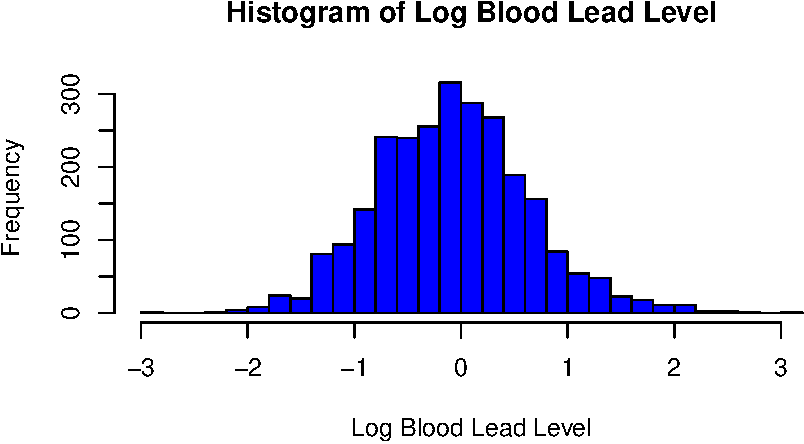
\includegraphics[width=1\textwidth,height=\textheight]{book/exploratory_analysis_files/figure-pdf/unnamed-chunk-9-1.pdf}
\end{center}

If we want to polish this figure, we can use some of the other optional
arguments \index{plots!extra arguments} to the \texttt{hist()} function.
For example, we may want to update the text
\texttt{log(nhanes\_df\$lead)} in the title and x-axis. In the following
code, we update the color, labels, and number of bins for the plot. The
function \texttt{colors()} returns all recognized colors in R. The
argument \texttt{breaks} specifies the number of bins to use to create
the histogram, \texttt{col} specifies the color, \texttt{main} specifies
the title of the plot, and \texttt{xlab} specifies the x-axis label
(using \texttt{ylab} would specify the y-axis label). Read the
documentation \texttt{?hist} for the full list of arguments available.

\begin{Shaded}
\begin{Highlighting}[]
\FunctionTok{hist}\NormalTok{(}\FunctionTok{log}\NormalTok{(nhanes\_df}\SpecialCharTok{$}\NormalTok{LEAD), }\AttributeTok{breaks =} \DecValTok{30}\NormalTok{, }\AttributeTok{col =} \StringTok{"blue"}\NormalTok{, }
     \AttributeTok{main =} \StringTok{"Histogram of Log Blood Lead Level"}\NormalTok{,}
     \AttributeTok{xlab =} \StringTok{"Log Blood Lead Level"}\NormalTok{)}
\end{Highlighting}
\end{Shaded}

\begin{center}
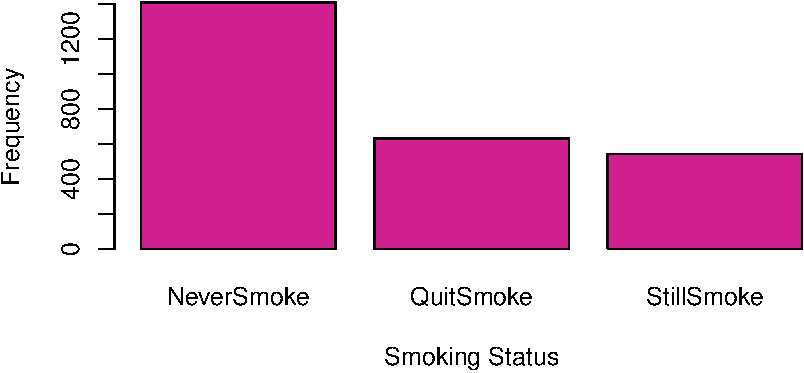
\includegraphics[width=1\textwidth,height=\textheight]{book/exploratory_analysis_files/figure-pdf/unnamed-chunk-10-1.pdf}
\end{center}

For categorical columns, we may want to plot the counts in each category
using a barplot\index{plots!barplot}. The function
\texttt{barplot()}\index{R functions!barplot()@\texttt{barplot()}} asks
us to specify the \texttt{names} and \texttt{heights} of the bars. To do
so, we need to store the counts for each category. Again, we update the
color and labels.

\begin{Shaded}
\begin{Highlighting}[]
\NormalTok{smoke\_counts }\OtherTok{\textless{}{-}} \FunctionTok{table}\NormalTok{(nhanes\_df}\SpecialCharTok{$}\NormalTok{SMOKE)}
\FunctionTok{barplot}\NormalTok{(}\AttributeTok{height =}\NormalTok{ smoke\_counts, }\AttributeTok{names =} \FunctionTok{names}\NormalTok{(smoke\_counts), }
        \AttributeTok{col =} \StringTok{"violetred"}\NormalTok{, }\AttributeTok{xlab=}\StringTok{"Smoking Status"}\NormalTok{, }\AttributeTok{ylab=}\StringTok{"Frequency"}\NormalTok{)}
\end{Highlighting}
\end{Shaded}

\begin{center}
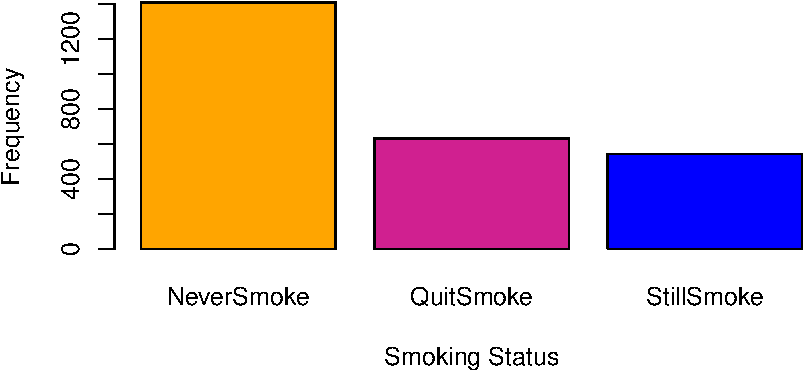
\includegraphics[width=1\textwidth,height=\textheight]{book/exploratory_analysis_files/figure-pdf/unnamed-chunk-11-1.pdf}
\end{center}

With a barplot, we can even specify a different color for each bar. To
do so, \texttt{col} must be a vector of specified colors with the same
length as the number of categories.

\begin{Shaded}
\begin{Highlighting}[]
\FunctionTok{barplot}\NormalTok{(}\AttributeTok{height =}\NormalTok{ smoke\_counts, }\AttributeTok{names =} \FunctionTok{names}\NormalTok{(smoke\_counts), }
        \AttributeTok{col =} \FunctionTok{c}\NormalTok{(}\StringTok{"orange"}\NormalTok{, }\StringTok{"violetred"}\NormalTok{, }\StringTok{"blue"}\NormalTok{),}
        \AttributeTok{xlab =} \StringTok{"Smoking Status"}\NormalTok{, }\AttributeTok{ylab =} \StringTok{"Frequency"}\NormalTok{)}
\end{Highlighting}
\end{Shaded}

\begin{center}
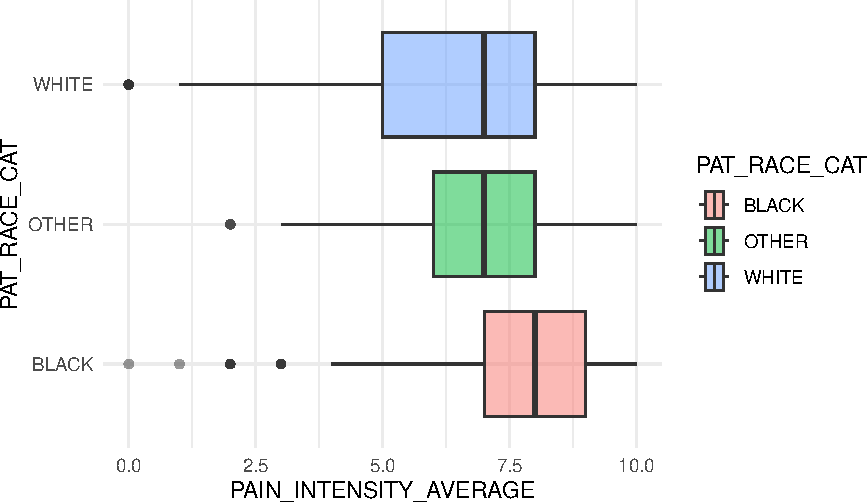
\includegraphics[width=1\textwidth,height=\textheight]{book/exploratory_analysis_files/figure-pdf/unnamed-chunk-12-1.pdf}
\end{center}

\subsection{Practice Question}\label{practice-question-6}

Recreate the barplot in Figure~\ref{fig-lead-quantile-bar-plot} below
showing the proportion of values in each \texttt{LEAD\_QUANTILE}
category.

\begin{figure}

\centering{

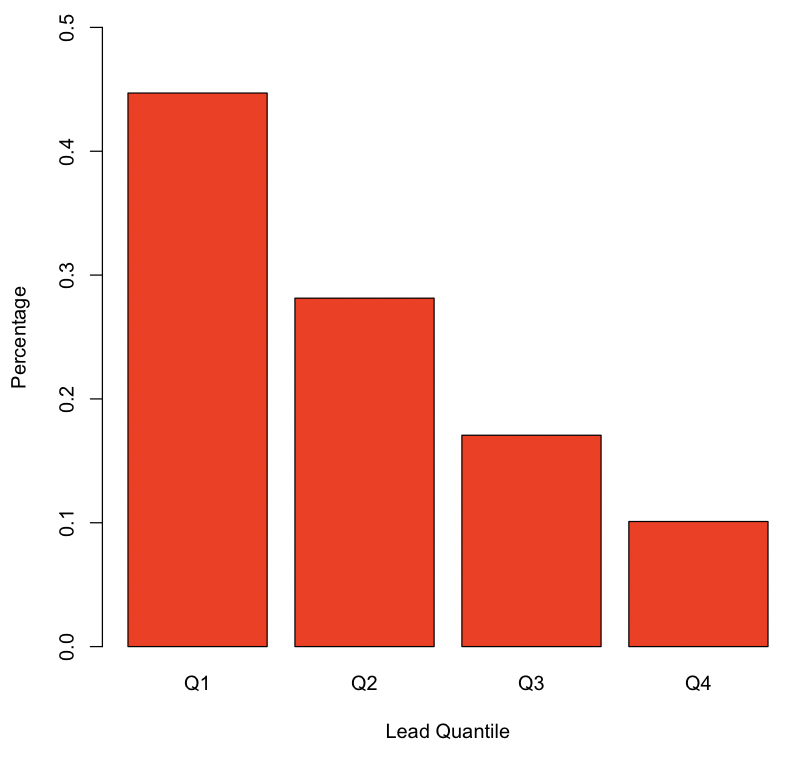
\includegraphics[width=0.7\textwidth,height=\textheight]{book/images/exploratory_analysis/lead-quantile-bar-plot.png}

}

\caption{\label{fig-lead-quantile-bar-plot}Lead Quantile Barplot.}

\end{figure}%

\begin{Shaded}
\begin{Highlighting}[]
\CommentTok{\# Insert your solution here:}
\end{Highlighting}
\end{Shaded}

\section{\texorpdfstring{Bivariate Distributions
\index{bivariate distributions}}{Bivariate Distributions }}\label{bivariate-distributions}

We now turn our attention to relationships among multiple columns. When
we have two categorical columns, we can use the \texttt{table()}
function to find the counts across all combinations. For example, we
look at the distribution of smoking status levels by sex. We observe
that a higher percentage of female participants have never smoked.

\begin{Shaded}
\begin{Highlighting}[]
\FunctionTok{table}\NormalTok{(nhanes\_df}\SpecialCharTok{$}\NormalTok{SMOKE, nhanes\_df}\SpecialCharTok{$}\NormalTok{SEX)}
\CommentTok{\#\textgreater{}             }
\CommentTok{\#\textgreater{}              Male Female}
\CommentTok{\#\textgreater{}   NeverSmoke  596    815}
\CommentTok{\#\textgreater{}   QuitSmoke   390    241}
\CommentTok{\#\textgreater{}   StillSmoke  324    218}
\end{Highlighting}
\end{Shaded}

To look at the sample distribution of a continuous column stratified by
a categorical column, we can call the \texttt{summary()} function for
each subset of the data. In the subsequent code, we look at the
distribution of blood lead level by sex and observe higher blood lead
levels in male observations.

\begin{Shaded}
\begin{Highlighting}[]
\FunctionTok{summary}\NormalTok{(nhanes\_df}\SpecialCharTok{$}\NormalTok{LEAD[nhanes\_df}\SpecialCharTok{$}\NormalTok{SEX }\SpecialCharTok{==} \StringTok{"Female"}\NormalTok{])}
\CommentTok{\#\textgreater{}    Min. 1st Qu.  Median    Mean 3rd Qu.    Max. }
\CommentTok{\#\textgreater{}    0.10    0.47    0.77    0.98    1.21    8.67}
\FunctionTok{summary}\NormalTok{(nhanes\_df}\SpecialCharTok{$}\NormalTok{LEAD[nhanes\_df}\SpecialCharTok{$}\NormalTok{SEX }\SpecialCharTok{==} \StringTok{"Male"}\NormalTok{])}
\CommentTok{\#\textgreater{}    Min. 1st Qu.  Median    Mean 3rd Qu.    Max. }
\CommentTok{\#\textgreater{}    0.05    0.70    1.09    1.46    1.66   22.01}
\end{Highlighting}
\end{Shaded}

We can also observe this visually through a
boxplot\index{plots!boxplot}. When given one categorical column and one
continuous column, the
\texttt{plot()}\index{R functions!plot()@\texttt{plot()}} function
creates a boxplot. By default, the first argument is the x-axis and the
second argument is the y-axis.

\begin{Shaded}
\begin{Highlighting}[]
\FunctionTok{plot}\NormalTok{(nhanes\_df}\SpecialCharTok{$}\NormalTok{SEX, }\FunctionTok{log}\NormalTok{(nhanes\_df}\SpecialCharTok{$}\NormalTok{LEAD), }\AttributeTok{ylab =} \StringTok{"Log Blood Lead Level"}\NormalTok{, }
     \AttributeTok{xlab =} \StringTok{"Sex"}\NormalTok{)}
\end{Highlighting}
\end{Shaded}

\begin{center}
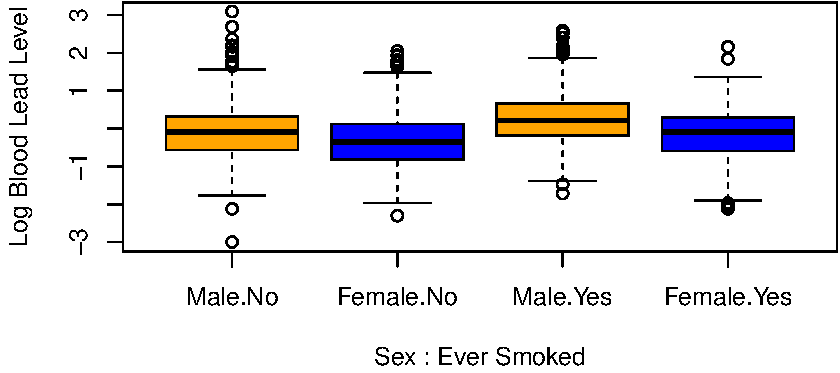
\includegraphics[width=1\textwidth,height=\textheight]{book/exploratory_analysis_files/figure-pdf/unnamed-chunk-16-1.pdf}
\end{center}

Alternatively, we can use the
\texttt{boxplot()}\index{R functions!boxplot()@\texttt{boxplot()}}
function, which can be passed a formula. A formula is a string
representation of how to group the data, where the left-hand side is the
continuous column, and the right-hand side is one or more categorical
columns to group by. In the following case, we group by multiple
columns, \texttt{SEX} and \texttt{EVER\_SMOKE}, so our formula is
\texttt{log(LEAD)\ \textasciitilde{}\ SEX\ +\ EVER\_SMOKE}. The second
argument to the function specifies the data. We specify the column
colors to show the link between the boxplots shown.

\begin{Shaded}
\begin{Highlighting}[]
\FunctionTok{boxplot}\NormalTok{(}\FunctionTok{log}\NormalTok{(LEAD) }\SpecialCharTok{\textasciitilde{}}\NormalTok{ SEX }\SpecialCharTok{+}\NormalTok{ EVER\_SMOKE, }\AttributeTok{data =}\NormalTok{ nhanes\_df, }
        \AttributeTok{col=}\FunctionTok{c}\NormalTok{(}\StringTok{"orange"}\NormalTok{, }\StringTok{"blue"}\NormalTok{, }\StringTok{"orange"}\NormalTok{, }\StringTok{"blue"}\NormalTok{),}
        \AttributeTok{xlab =} \StringTok{"Sex : Ever Smoked"}\NormalTok{, }\AttributeTok{ylab =} \StringTok{"Log Blood Lead Level"}\NormalTok{)}
\end{Highlighting}
\end{Shaded}

\begin{center}
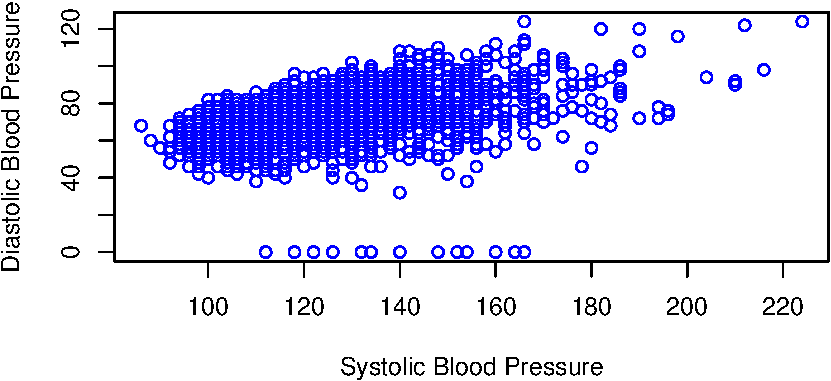
\includegraphics[width=1\textwidth,height=\textheight]{book/exploratory_analysis_files/figure-pdf/unnamed-chunk-17-1.pdf}
\end{center}

To visualize the bivariate distributions between two continuous columns,
we can use scatter plots\index{plots!scatter plot}. To create a scatter
plot, we use the
\texttt{plot()}\index{R functions!plot()@\texttt{plot()}} function
again. We use this function to show the relationship between systolic
and diastolic blood pressure.

\begin{Shaded}
\begin{Highlighting}[]
\FunctionTok{plot}\NormalTok{(nhanes\_df}\SpecialCharTok{$}\NormalTok{SBP1, nhanes\_df}\SpecialCharTok{$}\NormalTok{DBP1, }\AttributeTok{col =} \StringTok{"blue"}\NormalTok{, }
    \AttributeTok{xlab =} \StringTok{"Systolic Blood Pressure"}\NormalTok{,}
    \AttributeTok{ylab =} \StringTok{"Diastolic Blood Pressure"}\NormalTok{)}
\end{Highlighting}
\end{Shaded}

\begin{center}
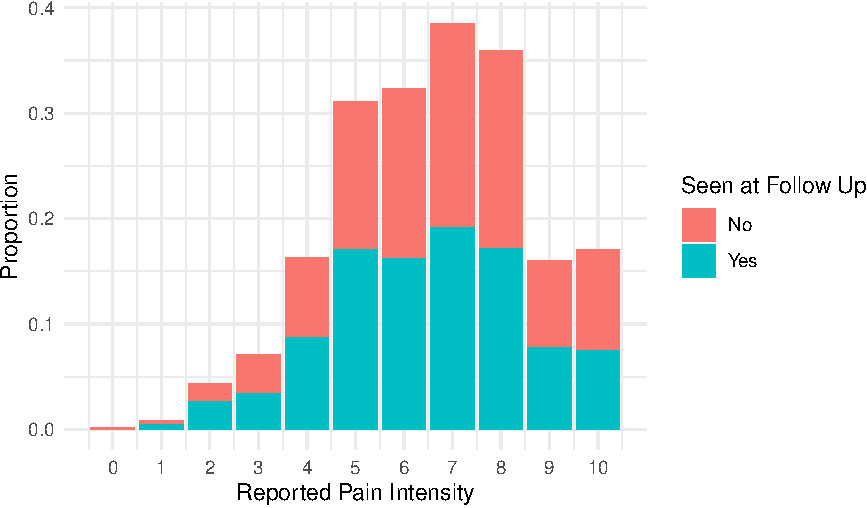
\includegraphics[width=1\textwidth,height=\textheight]{book/exploratory_analysis_files/figure-pdf/unnamed-chunk-18-1.pdf}
\end{center}

The two measures of blood pressure look highly correlated. We can
calculate their Pearson and Spearman correlation using the
\texttt{cor()}\index{R functions!cor()@\texttt{cor()}} function. The
default method is the Pearson correlation, but we can also calculate the
Kendall or Spearman correlation by specifying the method.

\begin{Shaded}
\begin{Highlighting}[]
\FunctionTok{cor}\NormalTok{(nhanes\_df}\SpecialCharTok{$}\NormalTok{SBP1, nhanes\_df}\SpecialCharTok{$}\NormalTok{DBP1)}
\CommentTok{\#\textgreater{} [1] 0.417}
\FunctionTok{cor}\NormalTok{(nhanes\_df}\SpecialCharTok{$}\NormalTok{SBP1, nhanes\_df}\SpecialCharTok{$}\NormalTok{DBP1, }\AttributeTok{method =} \StringTok{"spearman"}\NormalTok{)}
\CommentTok{\#\textgreater{} [1] 0.471}
\end{Highlighting}
\end{Shaded}

We may also want to add some extra information to our plot. This time,
instead of specifying the color manually, we use the column
\texttt{hyp}, an indicator for hypertension, to specify the color. We
have to make sure this vector is a factor for R to color by group.
Additionally, we add a blue vertical and horizontal line using the
\texttt{abline()}\index{R functions!abline()@\texttt{abline()}} function
to mark cutoffs for hypertension. Even though this function is called
after \texttt{plot()}, the lines are automatically added to the current
plot. We can see that most of those with hypertension have systolic or
diastolic blood pressure measurements above this threshold.

\begin{Shaded}
\begin{Highlighting}[]
\FunctionTok{plot}\NormalTok{(nhanes\_df}\SpecialCharTok{$}\NormalTok{SBP1, nhanes\_df}\SpecialCharTok{$}\NormalTok{DBP1, }\AttributeTok{col =} \FunctionTok{as.factor}\NormalTok{(nhanes\_df}\SpecialCharTok{$}\NormalTok{HYP), }
     \AttributeTok{xlab =} \StringTok{"Systolic Blood Pressure"}\NormalTok{,}
     \AttributeTok{ylab =} \StringTok{"Diastolic Blood Pressure"}\NormalTok{)}
\FunctionTok{abline}\NormalTok{(}\AttributeTok{v =} \DecValTok{130}\NormalTok{, }\AttributeTok{col =} \StringTok{"blue"}\NormalTok{)}
\FunctionTok{abline}\NormalTok{(}\AttributeTok{h =} \DecValTok{80}\NormalTok{, }\AttributeTok{col =} \StringTok{"blue"}\NormalTok{)}
\end{Highlighting}
\end{Shaded}

\begin{center}
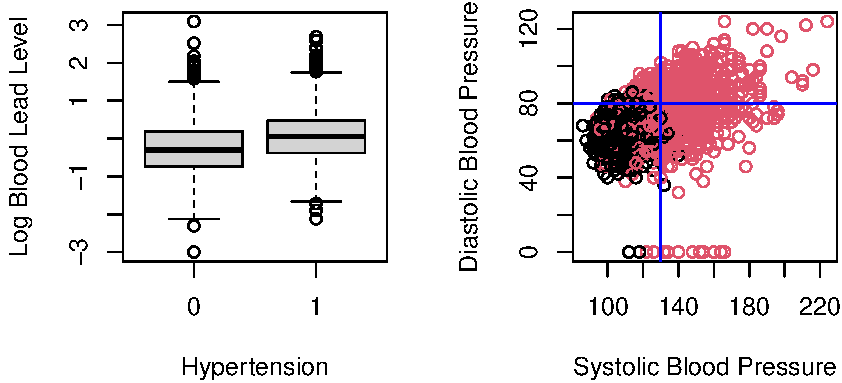
\includegraphics[width=1\textwidth,height=\textheight]{book/exploratory_analysis_files/figure-pdf/unnamed-chunk-20-1.pdf}
\end{center}

\newpage

The previous plots are all displayed as a single
figure\index{plots!combining plots}. If we want to display multiple
plots next to each other, we can specify the graphical parameters using
the \texttt{par()}\index{R functions!par()@\texttt{par()}} function by
updating the argument \texttt{mfrow\ =\ c(nrow,\ ncol)} with the number
of columns and rows we would like to use for our figures. We use this to
display the distribution of log blood lead level between those with and
without hypertension next to the previous plot.

\begin{Shaded}
\begin{Highlighting}[]
\FunctionTok{par}\NormalTok{(}\AttributeTok{mfrow =} \FunctionTok{c}\NormalTok{(}\DecValTok{1}\NormalTok{, }\DecValTok{2}\NormalTok{))}

\CommentTok{\# boxplot}
\FunctionTok{boxplot}\NormalTok{(}\FunctionTok{log}\NormalTok{(LEAD) }\SpecialCharTok{\textasciitilde{}}\NormalTok{ HYP, }\AttributeTok{data =}\NormalTok{ nhanes\_df, }\AttributeTok{xlab =} \StringTok{"Hypertension"}\NormalTok{, }
        \AttributeTok{ylab =} \StringTok{"Log Blood Lead Level"}\NormalTok{)}

\CommentTok{\# scatter plot}
\FunctionTok{plot}\NormalTok{(nhanes\_df}\SpecialCharTok{$}\NormalTok{SBP1, nhanes\_df}\SpecialCharTok{$}\NormalTok{DBP1, }\AttributeTok{col =} \FunctionTok{as.factor}\NormalTok{(nhanes\_df}\SpecialCharTok{$}\NormalTok{HYP), }
     \AttributeTok{xlab =} \StringTok{"Systolic Blood Pressure"}\NormalTok{,}
     \AttributeTok{ylab =} \StringTok{"Diastolic Blood Pressure"}\NormalTok{)}
\FunctionTok{abline}\NormalTok{(}\AttributeTok{v =} \DecValTok{130}\NormalTok{, }\AttributeTok{col =} \StringTok{"blue"}\NormalTok{)}
\FunctionTok{abline}\NormalTok{(}\AttributeTok{h =} \DecValTok{80}\NormalTok{, }\AttributeTok{col =} \StringTok{"blue"}\NormalTok{)}
\end{Highlighting}
\end{Shaded}

\begin{center}
\includegraphics[width=1\textwidth,height=\textheight]{book/exploratory_analysis_files/figure-pdf/unnamed-chunk-21-1.pdf}
\end{center}

We then reset to only display a single plot for future images using the
\texttt{par()} function again.

\begin{Shaded}
\begin{Highlighting}[]
\FunctionTok{par}\NormalTok{(}\AttributeTok{mfrow =} \FunctionTok{c}\NormalTok{(}\DecValTok{1}\NormalTok{, }\DecValTok{1}\NormalTok{))}
\end{Highlighting}
\end{Shaded}

\subsection{Practice Question}\label{practice-question-7}

Recreate the three boxplots in Figure~\ref{fig-box-plot} (one for each
education level) of income by BMI category and arrange them next to each
other using the \texttt{par()} function.

\begin{figure}

\centering{

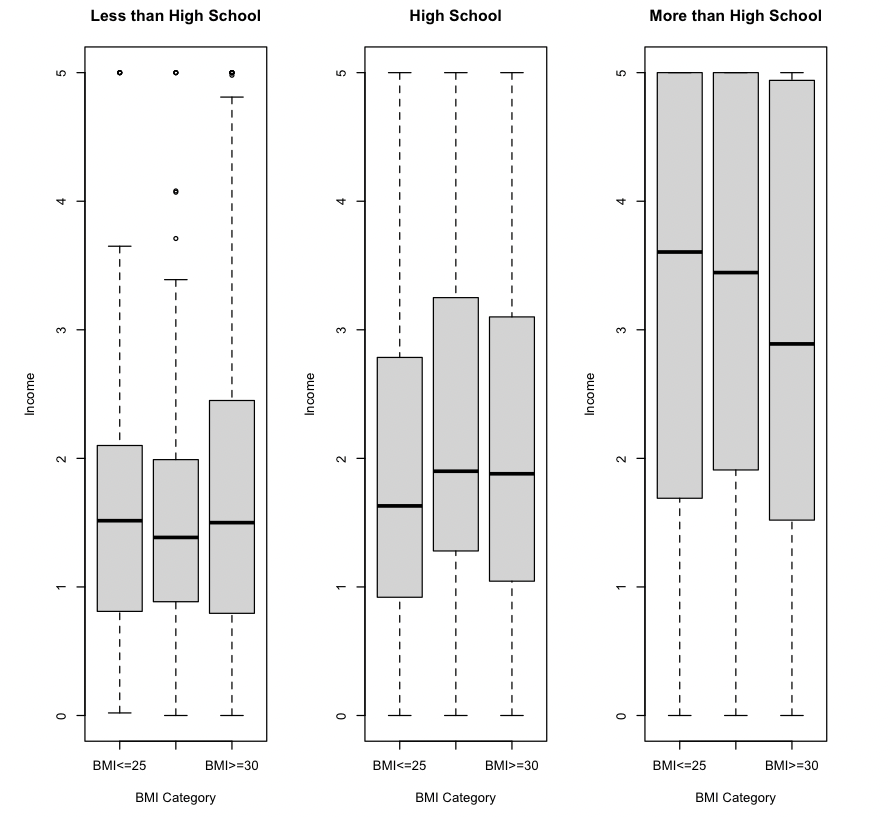
\includegraphics[width=1\textwidth,height=\textheight]{book/images/exploratory_analysis/box-plot.png}

}

\caption{\label{fig-box-plot}Boxplot Example.}

\end{figure}%

\begin{Shaded}
\begin{Highlighting}[]
\CommentTok{\# Insert your solution here:}
\end{Highlighting}
\end{Shaded}

\section{\texorpdfstring{Autogenerated Plots
\index{plots:data summary plots}}{Autogenerated Plots }}\label{autogenerated-plots}

In the previous sections, we learned some new functions for visualizing
the relationship between columns. The
\textbf{GGally}\index{R packages!GGally} package contains some useful
functions for looking at multiple univariate and bivariate relationships
at the same time, such as the
\texttt{ggpairs()}\index{R functions!ggpairs()@\texttt{ggpairs()}}
function. The function \texttt{ggpairs()} takes the data as its first
argument. By default, it plots the pairwise distributions for all
columns, but we can also specify to only select a subset of columns
using the \texttt{columns} argument. You can see in the following
example that it plots barplots and density plots for each univariate
sample distribution. It then plots the bivariate distributions and
calculates the Pearson correlation for all pairs of continuous columns.
That's a lot of information!

\begin{Shaded}
\begin{Highlighting}[]
\FunctionTok{ggpairs}\NormalTok{(nhanes\_df, }\AttributeTok{columns =} \FunctionTok{c}\NormalTok{(}\StringTok{"SEX"}\NormalTok{, }\StringTok{"AGE"}\NormalTok{, }\StringTok{"LEAD"}\NormalTok{, }\StringTok{"SBP1"}\NormalTok{, }\StringTok{"DBP1"}\NormalTok{))}
\end{Highlighting}
\end{Shaded}

\begin{center}
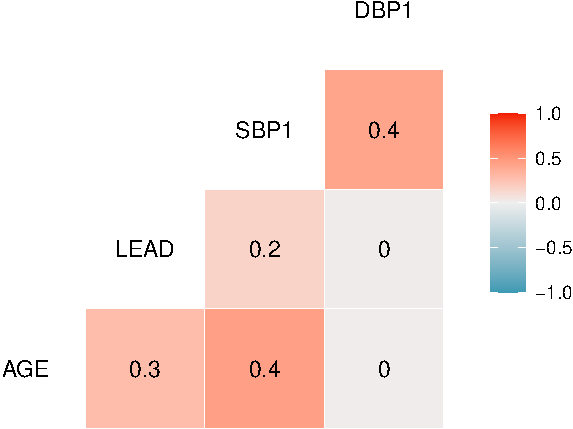
\includegraphics[width=1\textwidth,height=\textheight]{book/exploratory_analysis_files/figure-pdf/unnamed-chunk-24-1.pdf}
\end{center}

Another useful function in this package is the
\texttt{ggcorr()}\index{R functions!ggcorr()@\texttt{ggcorr()}}
function. This function takes in a data frame with only numeric columns
and displays the correlation between all pairs of columns, where the
color of each grid cell indicates the strength of the correlation. The
additional argument \texttt{label=TRUE} prints the actual correlation
value on each grid cell. This is a useful way to identify pairs of
strongly correlated columns. Note that we used the pipe operator again
to find the correlation on the continuous columns without saving this
subset of data.

\begin{Shaded}
\begin{Highlighting}[]
\NormalTok{nhanes\_df[, }\FunctionTok{c}\NormalTok{(}\StringTok{"AGE"}\NormalTok{, }\StringTok{"LEAD"}\NormalTok{, }\StringTok{"SBP1"}\NormalTok{, }\StringTok{"DBP1"}\NormalTok{)] }\SpecialCharTok{|\textgreater{}}
  \FunctionTok{ggcorr}\NormalTok{(}\AttributeTok{label =} \ConstantTok{TRUE}\NormalTok{)}
\end{Highlighting}
\end{Shaded}

\begin{center}
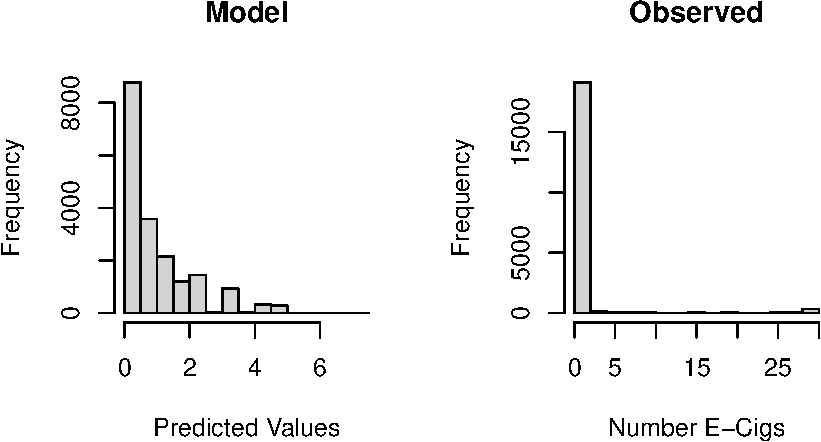
\includegraphics[width=1\textwidth,height=\textheight]{book/exploratory_analysis_files/figure-pdf/unnamed-chunk-25-1.pdf}
\end{center}

\section{\texorpdfstring{Tables \index{tables}}{Tables }}\label{tables}

Another useful way to display information about your data is through
tables. For example, it is standard practice in articles to have the
first table in the paper give information about the study sample, such
as the mean and standard deviation for all continuous columns and the
proportions for categorical columns. The \textbf{gt} package
\index{R packages!gt} is designed to create polished tables that can
include footnotes, titles, column labels, etc. The \textbf{gtsummary}
package \index{R packages!gtsummary} is an extension of this package
that can create summary tables. We focus on the latter but come back to
creating nice tables in Chapter~\ref{sec-quarto}.

To start, we create a gt object (a special type of table) of the first
six rows of our data using the
\texttt{gt()}\index{R functions!gt()@\texttt{gt()}} function. You can
see the difference in the formatting as opposed to printing the data.

\begin{Shaded}
\begin{Highlighting}[]
\FunctionTok{gt}\NormalTok{(}\FunctionTok{head}\NormalTok{(nhanes\_df[, }\FunctionTok{c}\NormalTok{(}\StringTok{"ID"}\NormalTok{, }\StringTok{"AGE"}\NormalTok{, }\StringTok{"SEX"}\NormalTok{, }\StringTok{"RACE"}\NormalTok{)])) }
\end{Highlighting}
\end{Shaded}

\begin{longtable*}{rrcc}
\toprule
ID & AGE & SEX & RACE \\ 
\midrule\addlinespace[2.5pt]
93711 & 56 & Male & Other Race \\ 
93713 & 67 & Male & Non-Hispanic White \\ 
93716 & 61 & Male & Other Race \\ 
93717 & 22 & Male & Non-Hispanic White \\ 
93721 & 60 & Female & Mexican American \\ 
93722 & 60 & Female & Non-Hispanic White \\ 
\bottomrule
\end{longtable*}

We now show you how to use the
\texttt{tbl\_summary()}\index{R functions!tbl\textunderscore summary()@\texttt{tbl\textunderscore summary()}}
function in the \textbf{gtsummary} package\index{tables!summary tables}.
The first argument to this function is again the data frame. By default,
this function summarizes all the columns in the data. Instead, we use
the \texttt{include} argument to specify a list of columns to include.
We then pipe this output to the function
\texttt{as\_gt()}\index{R functions!as\textunderscore gt()@\texttt{as\textunderscore gt()}},
which creates a gt table from the summary output. Note that the table
computes the total number of observations and the proportions for
categorical columns and the median and interquartile range for
continuous columns.

\begin{Shaded}
\begin{Highlighting}[]
\FunctionTok{tbl\_summary}\NormalTok{(nhanes\_df, }
            \AttributeTok{include =} \FunctionTok{c}\NormalTok{(}\StringTok{"SEX"}\NormalTok{, }\StringTok{"RACE"}\NormalTok{, }\StringTok{"AGE"}\NormalTok{, }\StringTok{"EDUCATION"}\NormalTok{, }\StringTok{"SMOKE"}\NormalTok{, }
                        \StringTok{"BMI\_CAT"}\NormalTok{, }\StringTok{"LEAD"}\NormalTok{, }\StringTok{"SBP1"}\NormalTok{, }\StringTok{"DBP1"}\NormalTok{, }\StringTok{"HYP"}\NormalTok{)) }\SpecialCharTok{|\textgreater{}}
  \FunctionTok{as\_gt}\NormalTok{()}
\end{Highlighting}
\end{Shaded}

\setlength{\LTpost}{0mm}
\begin{longtable*}{lc}
\toprule
\textbf{Characteristic} & \textbf{N = 2,584}\textsuperscript{\textit{1}} \\ 
\midrule\addlinespace[2.5pt]
SEX &  \\ 
    Male & 1,310 (51\%) \\ 
    Female & 1,274 (49\%) \\ 
RACE &  \\ 
    Mexican American & 358 (14\%) \\ 
    Other Hispanic & 225 (8.7\%) \\ 
    Non-Hispanic White & 992 (38\%) \\ 
    Non-Hispanic Black & 568 (22\%) \\ 
    Other Race & 441 (17\%) \\ 
AGE & 48 (33, 62) \\ 
EDUCATION &  \\ 
    LessThanHS & 373 (14\%) \\ 
    HS & 593 (23\%) \\ 
    MoreThanHS & 1,618 (63\%) \\ 
SMOKE &  \\ 
    NeverSmoke & 1,411 (55\%) \\ 
    QuitSmoke & 631 (24\%) \\ 
    StillSmoke & 542 (21\%) \\ 
BMI\_CAT &  \\ 
    BMI<=25 & 663 (26\%) \\ 
    25<BMI<30 & 808 (31\%) \\ 
    BMI>=30 & 1,113 (43\%) \\ 
LEAD & 0.93 (0.56, 1.44) \\ 
SBP1 & 122 (112, 134) \\ 
DBP1 & 72 (66, 80) \\ 
HYP & 1,451 (56\%) \\ 
\bottomrule
\end{longtable*}
\begin{minipage}{\linewidth}
\textsuperscript{\textit{1}}n (\%); Median (IQR)\\
\end{minipage}

We can update our table by changing some of its arguments. This time, we
specify that we want to stratify our table by hypertension status so
that the table summarizes the data by this grouping. Additionally, we
change how continuous columns are summarized by specifying that we want
to report the mean and standard deviation instead of the median and
interquartile range. We do this using the \texttt{statistic} argument.
The documentation for the \texttt{tbl\_summary()} function can help you
format this argument depending on which statistics you would like to
display.

\begin{Shaded}
\begin{Highlighting}[]
\FunctionTok{tbl\_summary}\NormalTok{(nhanes\_df, }
            \AttributeTok{include =} \FunctionTok{c}\NormalTok{(}\StringTok{"SEX"}\NormalTok{, }\StringTok{"RACE"}\NormalTok{, }\StringTok{"AGE"}\NormalTok{, }\StringTok{"EDUCATION"}\NormalTok{, }\StringTok{"SMOKE"}\NormalTok{, }
                        \StringTok{"BMI\_CAT"}\NormalTok{, }\StringTok{"LEAD"}\NormalTok{, }\StringTok{"SBP1"}\NormalTok{, }\StringTok{"DBP1"}\NormalTok{, }\StringTok{"HYP"}\NormalTok{),}
            \AttributeTok{by =} \StringTok{"HYP"}\NormalTok{,}
            \AttributeTok{statistic =} \FunctionTok{list}\NormalTok{(}\FunctionTok{all\_continuous}\NormalTok{() }\SpecialCharTok{\textasciitilde{}} \StringTok{"\{mean\} (\{sd\})"}\NormalTok{)) }\SpecialCharTok{|\textgreater{}}
\FunctionTok{as\_gt}\NormalTok{() }
\end{Highlighting}
\end{Shaded}

\setlength{\LTpost}{0mm}
\begin{longtable*}{lcc}
\toprule
\textbf{Characteristic} & \textbf{0}, N = 1,133\textsuperscript{\textit{1}} & \textbf{1}, N = 1,451\textsuperscript{\textit{1}} \\ 
\midrule\addlinespace[2.5pt]
SEX &  &  \\ 
    Male & 472 (42\%) & 838 (58\%) \\ 
    Female & 661 (58\%) & 613 (42\%) \\ 
RACE &  &  \\ 
    Mexican American & 186 (16\%) & 172 (12\%) \\ 
    Other Hispanic & 104 (9.2\%) & 121 (8.3\%) \\ 
    Non-Hispanic White & 429 (38\%) & 563 (39\%) \\ 
    Non-Hispanic Black & 203 (18\%) & 365 (25\%) \\ 
    Other Race & 211 (19\%) & 230 (16\%) \\ 
AGE & 40 (15) & 55 (16) \\ 
EDUCATION &  &  \\ 
    LessThanHS & 151 (13\%) & 222 (15\%) \\ 
    HS & 250 (22\%) & 343 (24\%) \\ 
    MoreThanHS & 732 (65\%) & 886 (61\%) \\ 
SMOKE &  &  \\ 
    NeverSmoke & 678 (60\%) & 733 (51\%) \\ 
    QuitSmoke & 220 (19\%) & 411 (28\%) \\ 
    StillSmoke & 235 (21\%) & 307 (21\%) \\ 
BMI\_CAT &  &  \\ 
    BMI<=25 & 392 (35\%) & 271 (19\%) \\ 
    25<BMI<30 & 351 (31\%) & 457 (31\%) \\ 
    BMI>=30 & 390 (34\%) & 723 (50\%) \\ 
LEAD & 1.03 (1.15) & 1.37 (1.25) \\ 
SBP1 & 112 (10) & 134 (18) \\ 
DBP1 & 67 (9) & 77 (14) \\ 
\bottomrule
\end{longtable*}
\begin{minipage}{\linewidth}
\textsuperscript{\textit{1}}n (\%); Mean (SD)\\
\end{minipage}

Outside of the \textbf{gt} and \textbf{gtsummary} packages, another
common package used to create summary tables is the \textbf{tableone}
\index{R packages!tableone} package (Yoshida and Bartel 2022), which is
not covered in this book.

\section{Exercises}\label{exercises-2}

For these exercises, we continue using the \texttt{nhanes\_df} data.

\begin{enumerate}
\def\labelenumi{\arabic{enumi}.}
\item
  Using both numerical and graphical summaries, describe the
  distribution of the first diastolic blood pressure reading
  \texttt{DBP1} among study participants. Then, create a column called
  \texttt{INCOME\_CAT} with two categories: ``low'' for those whose
  income is at most 2 and ``not low'' otherwise, and examine the
  bivariate distribution of \texttt{DBP1} and \texttt{INCOME\_CAT}.
  Arrange the two plots next to each other. What do you notice?
\item
  Create a subset of the data containing only adults between the ages of
  20 and 55, inclusive. Then, explore how blood pressure varies by age
  and gender among this age group. Is there a visible trend in blood
  pressure with increasing age among either sex?
\item
  For males between the ages of 50 and 59, compare blood pressure across
  race as reported in the race column. Then, create a summary table
  stratified by the race column and report the mean, standard deviation,
  minimum, and maximum values for all continuous columns.
\item
  Recreate the plots in Figure~\ref{fig-education-over-time} and
  Figure~\ref{fig-bll-by-education}. Based on these plots, what trend do
  you expect to see in blood lead levels over time? Check your answer to
  the previous question by plotting these two columns against each
  other.
\end{enumerate}

\begin{figure}

\centering{

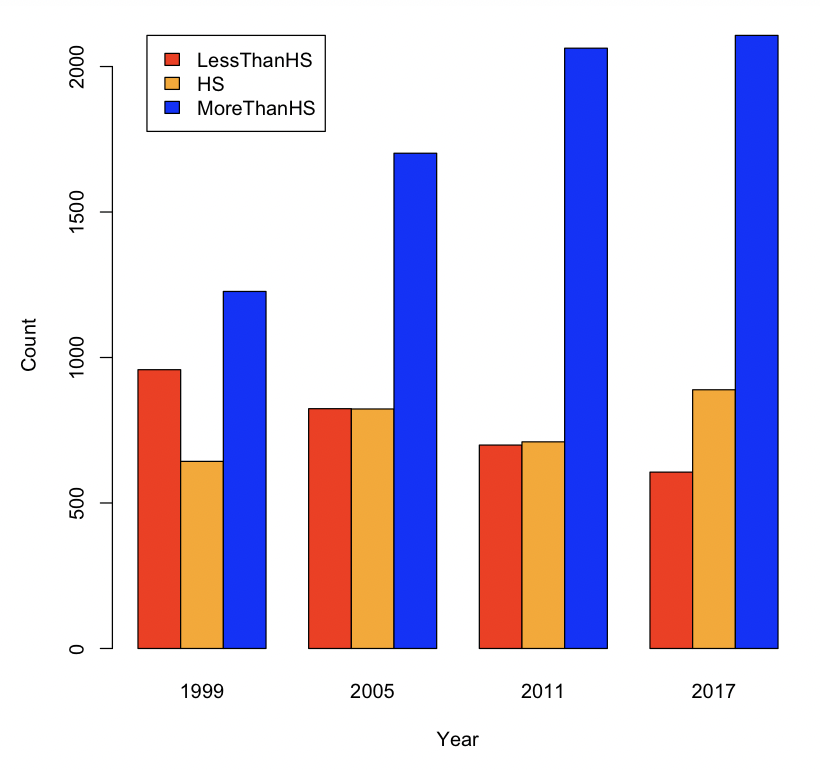
\includegraphics[width=0.8\textwidth,height=\textheight]{book/images/exploratory_analysis/education-over-time.png}

}

\caption{\label{fig-education-over-time}Education Levels Over Time.}

\end{figure}%

\begin{figure}

\centering{

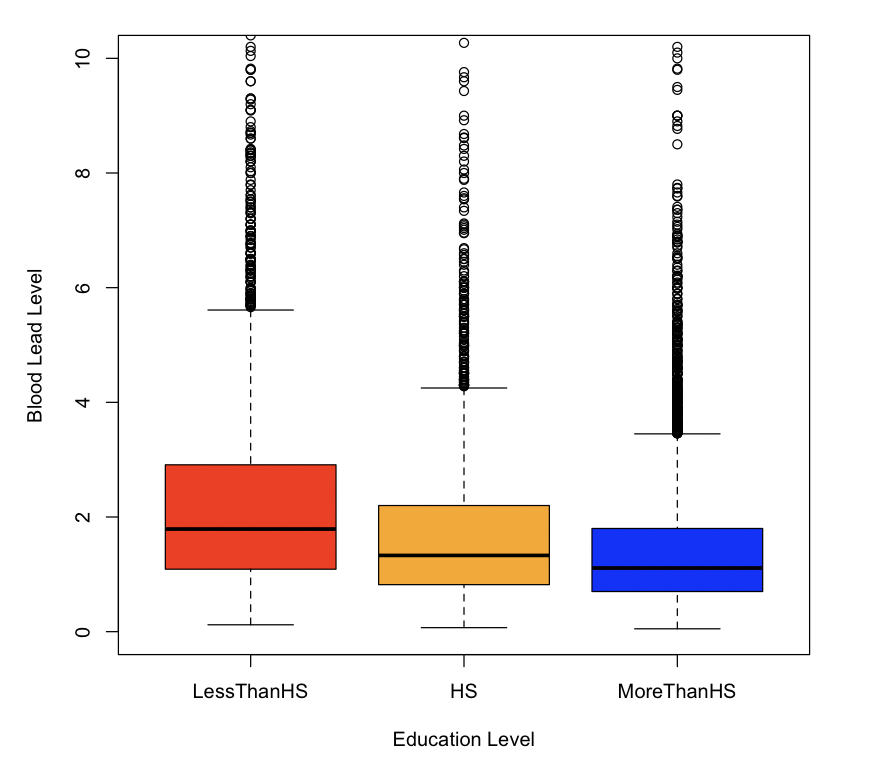
\includegraphics[width=0.8\textwidth,height=\textheight]{book/images/exploratory_analysis/bll-by-education.png}

}

\caption{\label{fig-bll-by-education}Blood Lead Level by Education
Level.}

\end{figure}%

\chapter{Data Transformations and
Summaries}\label{sec-transformations-summaries}

In this chapter, we introduce the \textbf{dplyr}\index{R packages!dplyr}
package (Wickham et al. 2023), which is part of the
\textbf{tidyverse}\index{R packages!tidyverse} group of packages, to
expand our tools in exploring and transforming our data. We learn how to
do some basic manipulations of data (e.g., adding or removing columns,
filtering data, arranging by one or multiple columns) as well as how to
summarize data (e.g., grouping by values, calculating summary
statistics). We also practice combining these operations using the pipe
operator \texttt{\%\textgreater{}\%} from the \textbf{tidyverse}. We use
the same sample of the National Health and Nutrition Examination Survey
(Centers for Disease Control and Prevention (CDC) 1999-2018)
\index{Datasets!NHANESSample@\texttt{NHANESSample}} as in
Chapter~\ref{sec-exploratory}.

\begin{Shaded}
\begin{Highlighting}[]
\FunctionTok{library}\NormalTok{(HDSinRdata)}
\FunctionTok{library}\NormalTok{(tidyverse)}

\FunctionTok{data}\NormalTok{(NHANESsample)}
\end{Highlighting}
\end{Shaded}

\section{Tibbles and Data Frames}\label{tibbles-and-data-frames}

Take a look at the class of \texttt{NHANESsample}. As we might expect,
the data is stored as a data frame.

\begin{Shaded}
\begin{Highlighting}[]
\FunctionTok{class}\NormalTok{(NHANESsample)}
\CommentTok{\#\textgreater{} [1] "data.frame"}
\end{Highlighting}
\end{Shaded}

However, \textbf{tidyverse} packages also work with another data
structure called a \textbf{tibble}\index{tibble}. A \textbf{tibble} has
all the properties of data frames that we have learned so far, but they
are a more modern version of a data frame. To convert our data to this
data structure, we use the
\texttt{as\_tibble()}\index{R functions!as\textunderscore tibble()@\texttt{as\textunderscore tibble()}}
function. In practice, there are only very slight differences between
the two data structures, and you generally do not need to convert data
frames to tibbles. In the following code chunks, we convert our data
from a data frame to a tibble and print the head of the data before
converting it back to a data frame and repeating. You can see the two
structures have a slightly different print statement but are otherwise
very similar.

\begin{Shaded}
\begin{Highlighting}[]
\NormalTok{nhanes\_df }\OtherTok{\textless{}{-}} \FunctionTok{as\_tibble}\NormalTok{(NHANESsample)}
\FunctionTok{print}\NormalTok{(}\FunctionTok{head}\NormalTok{(nhanes\_df))}
\CommentTok{\#\textgreater{} \# A tibble: 6 x 21}
\CommentTok{\#\textgreater{}      ID   AGE SEX    RACE     EDUCATION INCOME SMOKE  YEAR  LEAD BMI\_CAT}
\CommentTok{\#\textgreater{}   \textless{}dbl\textgreater{} \textless{}dbl\textgreater{} \textless{}fct\textgreater{}  \textless{}fct\textgreater{}    \textless{}fct\textgreater{}      \textless{}dbl\textgreater{} \textless{}fct\textgreater{} \textless{}dbl\textgreater{} \textless{}dbl\textgreater{} \textless{}fct\textgreater{}  }
\CommentTok{\#\textgreater{} 1     2    77 Male   Non{-}His\textasciitilde{} MoreThan\textasciitilde{}   5    Neve\textasciitilde{}  1999   5   BMI\textless{}=25}
\CommentTok{\#\textgreater{} 2     5    49 Male   Non{-}His\textasciitilde{} MoreThan\textasciitilde{}   5    Quit\textasciitilde{}  1999   1.6 25\textless{}BMI\textasciitilde{}}
\CommentTok{\#\textgreater{} 3    12    37 Male   Non{-}His\textasciitilde{} MoreThan\textasciitilde{}   4.93 Neve\textasciitilde{}  1999   2.4 BMI\textgreater{}=30}
\CommentTok{\#\textgreater{} 4    13    70 Male   Mexican\textasciitilde{} LessThan\textasciitilde{}   1.07 Quit\textasciitilde{}  1999   1.6 25\textless{}BMI\textasciitilde{}}
\CommentTok{\#\textgreater{} 5    14    81 Male   Non{-}His\textasciitilde{} LessThan\textasciitilde{}   2.67 Stil\textasciitilde{}  1999   5.5 25\textless{}BMI\textasciitilde{}}
\CommentTok{\#\textgreater{} 6    15    38 Female Non{-}His\textasciitilde{} MoreThan\textasciitilde{}   4.52 Stil\textasciitilde{}  1999   1.5 25\textless{}BMI\textasciitilde{}}
\CommentTok{\#\textgreater{} \# i 11 more variables: LEAD\_QUANTILE \textless{}fct\textgreater{}, HYP \textless{}dbl\textgreater{}, ALC \textless{}chr\textgreater{},}
\CommentTok{\#\textgreater{} \#   DBP1 \textless{}dbl\textgreater{}, DBP2 \textless{}dbl\textgreater{}, DBP3 \textless{}dbl\textgreater{}, DBP4 \textless{}dbl\textgreater{}, SBP1 \textless{}dbl\textgreater{},}
\CommentTok{\#\textgreater{} \#   SBP2 \textless{}dbl\textgreater{}, SBP3 \textless{}dbl\textgreater{}, SBP4 \textless{}dbl\textgreater{}}
\end{Highlighting}
\end{Shaded}

\begin{Shaded}
\begin{Highlighting}[]
\NormalTok{nhanes\_df }\OtherTok{\textless{}{-}} \FunctionTok{as.data.frame}\NormalTok{(nhanes\_df)}
\FunctionTok{print}\NormalTok{(}\FunctionTok{head}\NormalTok{(nhanes\_df))}
\CommentTok{\#\textgreater{}   ID AGE    SEX               RACE  EDUCATION INCOME      SMOKE YEAR}
\CommentTok{\#\textgreater{} 1  2  77   Male Non{-}Hispanic White MoreThanHS   5.00 NeverSmoke 1999}
\CommentTok{\#\textgreater{} 2  5  49   Male Non{-}Hispanic White MoreThanHS   5.00  QuitSmoke 1999}
\CommentTok{\#\textgreater{} 3 12  37   Male Non{-}Hispanic White MoreThanHS   4.93 NeverSmoke 1999}
\CommentTok{\#\textgreater{} 4 13  70   Male   Mexican American LessThanHS   1.07  QuitSmoke 1999}
\CommentTok{\#\textgreater{} 5 14  81   Male Non{-}Hispanic White LessThanHS   2.67 StillSmoke 1999}
\CommentTok{\#\textgreater{} 6 15  38 Female Non{-}Hispanic White MoreThanHS   4.52 StillSmoke 1999}
\CommentTok{\#\textgreater{}   LEAD   BMI\_CAT LEAD\_QUANTILE HYP ALC DBP1 DBP2 DBP3 DBP4 SBP1 SBP2}
\CommentTok{\#\textgreater{} 1  5.0   BMI\textless{}=25            Q4   0 Yes   58   56   56   NA  106   98}
\CommentTok{\#\textgreater{} 2  1.6 25\textless{}BMI\textless{}30            Q3   1 Yes   82   84   82   NA  122  122}
\CommentTok{\#\textgreater{} 3  2.4   BMI\textgreater{}=30            Q4   1 Yes  108   98  100   NA  182  172}
\CommentTok{\#\textgreater{} 4  1.6 25\textless{}BMI\textless{}30            Q3   1 Yes   78   62   70   NA  140  130}
\CommentTok{\#\textgreater{} 5  5.5 25\textless{}BMI\textless{}30            Q4   1 Yes   56   NA   58   64  142   NA}
\CommentTok{\#\textgreater{} 6  1.5 25\textless{}BMI\textless{}30            Q3   0 Yes   68   68   70   NA  106  112}
\CommentTok{\#\textgreater{}   SBP3 SBP4}
\CommentTok{\#\textgreater{} 1   98   NA}
\CommentTok{\#\textgreater{} 2  122   NA}
\CommentTok{\#\textgreater{} 3  176   NA}
\CommentTok{\#\textgreater{} 4  130   NA}
\CommentTok{\#\textgreater{} 5  134  138}
\CommentTok{\#\textgreater{} 6  106   NA}
\end{Highlighting}
\end{Shaded}

We mention tibbles here since some functions in the \textbf{tidyverse}
convert data frames to tibbles in their output. In particular, when we
later summarize over groups we can expect a tibble to be returned. It is
useful to be aware that our data may change data structure with such
functions and to know that we can always convert back if needed.

\section{\texorpdfstring{Subsetting Data \index{subsetting data}
\index{selecting data}
\index{filtering data}}{Subsetting Data   }}\label{subsetting-data}

In earlier chapters, we have seen how to select and filter data using
row and column indices as well as using the
\texttt{subset()}\index{R functions!subset()@\texttt{subset()}}
function. The \textbf{dplyr} package has its own functions that are
useful for subsetting data. The
\texttt{select()}\index{R functions!select()@\texttt{select()}} function
allows us to select a subset of columns: this function takes in the data
frame (or tibble) and the names or indices of the columns we want to
select. For example, if we only wanted to select the variables for race
and blood lead level, we could specify these two columns. To display the
result of this selection, we use the pipe operator
\texttt{\%\textgreater{}\%} \index{pipe operator} from the
\textbf{magittr} \index{R packages!magittr} package of the
\textbf{tidyverse}. Similar to the pipe operator
\texttt{\textbar{}\textgreater{}} in base R, the pipe operator
\texttt{\%\textgreater{}\%} takes the result on the left-hand side and
passes it as the first argument to the function on the right-hand side.
The following output shows that there are only two columns in the
filtered data.

\begin{Shaded}
\begin{Highlighting}[]
\FunctionTok{select}\NormalTok{(nhanes\_df, }\FunctionTok{c}\NormalTok{(RACE, LEAD)) }\SpecialCharTok{\%\textgreater{}\%} \FunctionTok{head}\NormalTok{()}
\CommentTok{\#\textgreater{}                 RACE LEAD}
\CommentTok{\#\textgreater{} 1 Non{-}Hispanic White  5.0}
\CommentTok{\#\textgreater{} 2 Non{-}Hispanic White  1.6}
\CommentTok{\#\textgreater{} 3 Non{-}Hispanic White  2.4}
\CommentTok{\#\textgreater{} 4   Mexican American  1.6}
\CommentTok{\#\textgreater{} 5 Non{-}Hispanic White  5.5}
\CommentTok{\#\textgreater{} 6 Non{-}Hispanic White  1.5}
\end{Highlighting}
\end{Shaded}

The \texttt{select()} function can also be used to \emph{remove} columns
by adding a negative sign in front of the vector of column names in its
arguments. For example, we keep all columns except \texttt{ID} and
\texttt{LEAD\_QUANTILE}. Note that in this case we have saved the
selected data back to our data frame \texttt{nhanes\_df}. Additionally,
this time we used a pipe operator to pipe the data to the select
function itself.

\begin{Shaded}
\begin{Highlighting}[]
\NormalTok{nhanes\_df }\OtherTok{\textless{}{-}}\NormalTok{ nhanes\_df }\SpecialCharTok{\%\textgreater{}\%} \FunctionTok{select}\NormalTok{(}\SpecialCharTok{{-}}\FunctionTok{c}\NormalTok{(ID, LEAD\_QUANTILE))}
\FunctionTok{names}\NormalTok{(nhanes\_df)}
\CommentTok{\#\textgreater{}  [1] "AGE"       "SEX"       "RACE"      "EDUCATION" "INCOME"   }
\CommentTok{\#\textgreater{}  [6] "SMOKE"     "YEAR"      "LEAD"      "BMI\_CAT"   "HYP"      }
\CommentTok{\#\textgreater{} [11] "ALC"       "DBP1"      "DBP2"      "DBP3"      "DBP4"     }
\CommentTok{\#\textgreater{} [16] "SBP1"      "SBP2"      "SBP3"      "SBP4"}
\end{Highlighting}
\end{Shaded}

While \texttt{select()} allows us to choose a subset of columns, the
\texttt{filter()}\index{R functions!filter()@\texttt{filter()}} function
allows us to choose a subset of rows. The \texttt{filter()} function
takes a data frame as the first argument and a vector of Booleans as the
second argument. This vector of Booleans can be generated using
conditional statements as we used in Chapter~\ref{sec-exploratory}. We
choose to filter the data to only observations after 2008.

\begin{Shaded}
\begin{Highlighting}[]
\NormalTok{nhanes\_df\_recent }\OtherTok{\textless{}{-}}\NormalTok{ nhanes\_df }\SpecialCharTok{\%\textgreater{}\%} \FunctionTok{filter}\NormalTok{(YEAR }\SpecialCharTok{\textgreater{}=} \DecValTok{2008}\NormalTok{)}
\end{Highlighting}
\end{Shaded}

We can combine conditions by using multiple \texttt{filter()} calls, by
creating a more complicated conditional statement using the \texttt{\&}
(and), \texttt{\textbar{}} (or), and \texttt{\%in\%} (in) operators, or
by separating the conditions with commas within filter. In the following
code, we demonstrate these three ways to filter the data to males
between 2008 and 2012. Note that the
\texttt{between()}\index{R functions!between()@\texttt{between()}}
function allows us to capture the logic
\texttt{YEAR\ \textgreater{}=\ 2008\ \&\ YEAR\ \textless{}=\ 2012}.

\begin{Shaded}
\begin{Highlighting}[]
\CommentTok{\# Example 1: multiple filter calls}
\NormalTok{nhanes\_df\_males1 }\OtherTok{\textless{}{-}}\NormalTok{ nhanes\_df }\SpecialCharTok{\%\textgreater{}\%}
  \FunctionTok{filter}\NormalTok{(YEAR }\SpecialCharTok{\textless{}=} \DecValTok{2012}\NormalTok{) }\SpecialCharTok{\%\textgreater{}\%}
  \FunctionTok{filter}\NormalTok{(YEAR }\SpecialCharTok{\textgreater{}=} \DecValTok{2008}\NormalTok{) }\SpecialCharTok{\%\textgreater{}\%}
  \FunctionTok{filter}\NormalTok{(SEX }\SpecialCharTok{==} \StringTok{"Male"}\NormalTok{)}

\CommentTok{\# Example 2: combine with \& operator}
\NormalTok{nhanes\_df\_males2 }\OtherTok{\textless{}{-}}\NormalTok{ nhanes\_df }\SpecialCharTok{\%\textgreater{}\%}
  \FunctionTok{filter}\NormalTok{((YEAR }\SpecialCharTok{\textless{}=} \DecValTok{2012}\NormalTok{) }\SpecialCharTok{\&}\NormalTok{ (YEAR }\SpecialCharTok{\textgreater{}=} \DecValTok{2008}\NormalTok{) }\SpecialCharTok{\&}\NormalTok{ (SEX }\SpecialCharTok{==} \StringTok{"Male"}\NormalTok{))}

\CommentTok{\# Example 3: combine into one filter call with commas}
\NormalTok{nhanes\_df\_males3 }\OtherTok{\textless{}{-}}\NormalTok{ nhanes\_df }\SpecialCharTok{\%\textgreater{}\%}
  \FunctionTok{filter}\NormalTok{(}\FunctionTok{between}\NormalTok{(YEAR, }\DecValTok{2008}\NormalTok{, }\DecValTok{2012}\NormalTok{), SEX }\SpecialCharTok{==} \StringTok{"Male"}\NormalTok{)}
\end{Highlighting}
\end{Shaded}

The use of parentheses in the previous code is especially important in
order to capture our desired logic. In all these examples, we broke our
code up into multiple lines, which makes it easier to read. A good rule
of thumb is to not go past 80 characters in a line, and R Studio
conveniently has a vertical gray line at this limit. To create a new
line, you can hit enter either after an operator (e.g.,
\texttt{\%\textgreater{}\%}, \texttt{+}, \texttt{\textbar{}}) or within
a set of unfinished brackets or parentheses. Either of these breaks lets
R know that your code is not finished yet.

Lastly, we can subset the data using the
\texttt{slice()}\index{R functions!slice()@\texttt{slice()}} function to
select a slice of rows by their index. The function takes in the dataset
and a vector of indices. In the following example, we find the first and
last rows of the data.

\begin{Shaded}
\begin{Highlighting}[]
\FunctionTok{slice}\NormalTok{(nhanes\_df, }\FunctionTok{c}\NormalTok{(}\DecValTok{1}\NormalTok{, }\FunctionTok{nrow}\NormalTok{(nhanes\_df)))}
\CommentTok{\#\textgreater{}   AGE  SEX               RACE  EDUCATION INCOME      SMOKE YEAR LEAD}
\CommentTok{\#\textgreater{} 1  77 Male Non{-}Hispanic White MoreThanHS   5.00 NeverSmoke 1999  5.0}
\CommentTok{\#\textgreater{} 2  38 Male Non{-}Hispanic White MoreThanHS   1.56 StillSmoke 2017  0.9}
\CommentTok{\#\textgreater{}   BMI\_CAT HYP ALC DBP1 DBP2 DBP3 DBP4 SBP1 SBP2 SBP3 SBP4}
\CommentTok{\#\textgreater{} 1 BMI\textless{}=25   0 Yes   58   56   56   NA  106   98   98   NA}
\CommentTok{\#\textgreater{} 2 BMI\textgreater{}=30   1 Yes   98   92   98   NA  150  146  148   NA}
\end{Highlighting}
\end{Shaded}

A few other useful slice functions are
\texttt{slice\_sample()}\index{R functions!slice\textunderscore sample()@\texttt{slice\textunderscore sample()}},
\texttt{slice\_max()}\index{R functions!slice\textunderscore max()@\texttt{slice\textunderscore max()}},
and
\texttt{slice\_min()}\index{R functions!slice\textunderscore min()@\texttt{slice\textunderscore min()}}.
The first takes in an argument \texttt{n} which specifies the number of
\emph{random} rows to sample from the data. For example, we could
randomly sample 100 rows from our data. The latter two allow us to
specify a column through the argument \texttt{order\_by} and return the
\texttt{n} rows with either the highest or lowest values in that column.
For example, we can find the three male observations from 2007 with the
highest and lowest blood lead levels and select a subset of columns to
display.

\begin{Shaded}
\begin{Highlighting}[]
\CommentTok{\# three male observations with highest blood lead level in 2007}
\NormalTok{nhanes\_df }\SpecialCharTok{\%\textgreater{}\%}
  \FunctionTok{filter}\NormalTok{(YEAR }\SpecialCharTok{==} \DecValTok{2007}\NormalTok{, SEX }\SpecialCharTok{==} \StringTok{"Male"}\NormalTok{) }\SpecialCharTok{\%\textgreater{}\%}
  \FunctionTok{select}\NormalTok{(}\FunctionTok{c}\NormalTok{(RACE, EDUCATION, SMOKE, LEAD, SBP1, DBP1)) }\SpecialCharTok{\%\textgreater{}\%}
  \FunctionTok{slice\_max}\NormalTok{(}\AttributeTok{order\_by =}\NormalTok{ LEAD, }\AttributeTok{n =} \DecValTok{3}\NormalTok{)}
\CommentTok{\#\textgreater{}                 RACE  EDUCATION      SMOKE LEAD SBP1 DBP1}
\CommentTok{\#\textgreater{} 1 Non{-}Hispanic Black LessThanHS NeverSmoke 33.1  106   66}
\CommentTok{\#\textgreater{} 2     Other Hispanic LessThanHS StillSmoke 26.8  106   72}
\CommentTok{\#\textgreater{} 3     Other Hispanic LessThanHS StillSmoke 25.7  112   60}

\CommentTok{\# three male observations with lowest blood lead level in 2007}
\NormalTok{nhanes\_df }\SpecialCharTok{\%\textgreater{}\%}
  \FunctionTok{filter}\NormalTok{(YEAR }\SpecialCharTok{==} \DecValTok{2007}\NormalTok{, SEX }\SpecialCharTok{==} \StringTok{"Male"}\NormalTok{) }\SpecialCharTok{\%\textgreater{}\%}
  \FunctionTok{select}\NormalTok{(}\FunctionTok{c}\NormalTok{(RACE, EDUCATION, SMOKE, LEAD, SBP1, DBP1)) }\SpecialCharTok{\%\textgreater{}\%}
  \FunctionTok{slice\_min}\NormalTok{(}\AttributeTok{order\_by =}\NormalTok{ LEAD, }\AttributeTok{n =} \DecValTok{3}\NormalTok{)}
\CommentTok{\#\textgreater{}                 RACE  EDUCATION      SMOKE  LEAD SBP1 DBP1}
\CommentTok{\#\textgreater{} 1 Non{-}Hispanic White LessThanHS NeverSmoke 0.177  114   80}
\CommentTok{\#\textgreater{} 2     Other Hispanic LessThanHS  QuitSmoke 0.280  122   62}
\CommentTok{\#\textgreater{} 3   Mexican American MoreThanHS  QuitSmoke 0.320  112   66}
\end{Highlighting}
\end{Shaded}

\subsection{Practice Question}\label{practice-question-8}

Filter the data to only those with an education level of more than HS
who report alcohol use. Then, select only the diastolic blood pressure
variables and display the fourth and tenth rows. Your result should
match the result in Figure~\ref{fig-filtering-and-selecting}.

\begin{figure}

\centering{

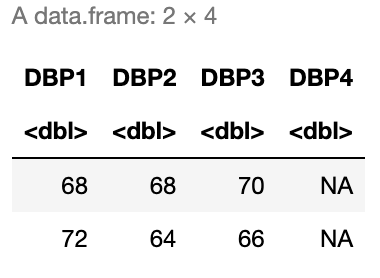
\includegraphics[width=2.08333in,height=\textheight]{book/images/data_transformations_summaries/filtering-and-selecting.png}

}

\caption{\label{fig-filtering-and-selecting}Filtering and Selecting
Data.}

\end{figure}%

\begin{Shaded}
\begin{Highlighting}[]
\CommentTok{\# Insert your solution here:}
\end{Highlighting}
\end{Shaded}

\section{\texorpdfstring{Updating Rows and Columns
\index{rename columns} \index{modify columns}
\index{sorting data}}{Updating Rows and Columns   }}\label{updating-rows-and-columns}

The next few functions we look at allow us to update the rows and
columns in our data. For example, the
\texttt{rename()}\index{R functions!rename()@\texttt{rename()}} function
allows us to change the names of columns. In the following code, we
change the name of \texttt{INCOME} to \texttt{PIR} since this variable
is the poverty income ratio and also update the name of \texttt{SMOKE}
to be \texttt{SMOKE\_STATUS}. When specifying these names, the new name
is on the left of the \texttt{=} and the old name is on the right.

\begin{Shaded}
\begin{Highlighting}[]
\NormalTok{nhanes\_df }\OtherTok{\textless{}{-}}\NormalTok{ nhanes\_df }\SpecialCharTok{\%\textgreater{}\%} \FunctionTok{rename}\NormalTok{(}\AttributeTok{PIR =}\NormalTok{ INCOME, }\AttributeTok{SMOKE\_STATUS =}\NormalTok{ SMOKE)}
\FunctionTok{names}\NormalTok{(nhanes\_df)}
\CommentTok{\#\textgreater{}  [1] "AGE"          "SEX"          "RACE"         "EDUCATION"   }
\CommentTok{\#\textgreater{}  [5] "PIR"          "SMOKE\_STATUS" "YEAR"         "LEAD"        }
\CommentTok{\#\textgreater{}  [9] "BMI\_CAT"      "HYP"          "ALC"          "DBP1"        }
\CommentTok{\#\textgreater{} [13] "DBP2"         "DBP3"         "DBP4"         "SBP1"        }
\CommentTok{\#\textgreater{} [17] "SBP2"         "SBP3"         "SBP4"}
\end{Highlighting}
\end{Shaded}

In the last chapter, we created a new variable called
\texttt{EVER\_SMOKE} based on the smoking status variable using the
\texttt{ifelse()}\index{R functions!ifelse()@\texttt{ifelse()}}
function. Recall that this function allows us to specify a condition,
and then two alternative values based on whether we meet or do not meet
this condition. We see that there are about 15,000 subjects in our data
who never smoked.

\begin{Shaded}
\begin{Highlighting}[]
\FunctionTok{ifelse}\NormalTok{(nhanes\_df}\SpecialCharTok{$}\NormalTok{SMOKE\_STATUS }\SpecialCharTok{==} \StringTok{"NeverSmoke"}\NormalTok{, }\StringTok{"No"}\NormalTok{, }\StringTok{"Yes"}\NormalTok{) }\SpecialCharTok{\%\textgreater{}\%} 
  \FunctionTok{table}\NormalTok{()}
\CommentTok{\#\textgreater{} .}
\CommentTok{\#\textgreater{}    No   Yes }
\CommentTok{\#\textgreater{} 15087 16178}
\end{Highlighting}
\end{Shaded}

Another useful function from the \textbf{tidyverse} is the
\texttt{case\_when()}\index{R functions!case\textunderscore when()@\texttt{case\textunderscore when()}}
function, which is an extension of the \texttt{ifelse()} function but
allows to specify more than two cases. We demonstrate this function to
show how we could relabel the levels of the \texttt{SMOKE\_STATUS}
column. For each condition, we use the right side of the
\texttt{\textasciitilde{}} to specify the value to be assigned when that
condition is TRUE.

\begin{Shaded}
\begin{Highlighting}[]
\FunctionTok{case\_when}\NormalTok{(nhanes\_df}\SpecialCharTok{$}\NormalTok{SMOKE\_STATUS }\SpecialCharTok{==} \StringTok{"NeverSmoke"} \SpecialCharTok{\textasciitilde{}} \StringTok{"Never Smoked"}\NormalTok{,}
\NormalTok{          nhanes\_df}\SpecialCharTok{$}\NormalTok{SMOKE\_STATUS }\SpecialCharTok{==} \StringTok{"QuitSmoke"} \SpecialCharTok{\textasciitilde{}} \StringTok{"Quit Smoking"}\NormalTok{,}
\NormalTok{          nhanes\_df}\SpecialCharTok{$}\NormalTok{SMOKE\_STATUS }\SpecialCharTok{==} 
            \StringTok{"StillSmoke"} \SpecialCharTok{\textasciitilde{}} \StringTok{"Current Smoker"}\NormalTok{) }\SpecialCharTok{\%\textgreater{}\%} 
  \FunctionTok{table}\NormalTok{()}
\CommentTok{\#\textgreater{} .}
\CommentTok{\#\textgreater{} Current Smoker   Never Smoked   Quit Smoking }
\CommentTok{\#\textgreater{}           7317          15087           8861}
\end{Highlighting}
\end{Shaded}

In the previous example, we did not store the columns we created. To do
so, we could use the \texttt{\$} operator or the \texttt{cbind()}
function. The \textbf{tidyverse} also includes an alternative function
to add columns called
\texttt{mutate()}\index{R functions!mutate()@\texttt{mutate()}}. This
function takes in a data frame and a set of columns with associated
names to add to the data or update. In the subsequent example, we create
the column \texttt{EVER\_SMOKE} and update the column
\texttt{SMOKE\_STATUS}. Within the \texttt{mutate()} function, we do not
have to use the \texttt{\$} operator to reference the column
\texttt{SMOKE\_STATUS}. Instead, we can specify just the column name,
and the function interprets it as that column.

\begin{Shaded}
\begin{Highlighting}[]
\NormalTok{nhanes\_df }\OtherTok{\textless{}{-}}\NormalTok{ nhanes\_df }\SpecialCharTok{\%\textgreater{}\%} 
  \FunctionTok{mutate}\NormalTok{(}\AttributeTok{EVER\_SMOKE =} \FunctionTok{ifelse}\NormalTok{(SMOKE\_STATUS }\SpecialCharTok{==} \StringTok{"NeverSmoke"}\NormalTok{, }
                             \StringTok{"No"}\NormalTok{, }\StringTok{"Yes"}\NormalTok{), }
         \AttributeTok{SMOKE\_STATUS =} 
           \FunctionTok{case\_when}\NormalTok{(SMOKE\_STATUS }\SpecialCharTok{==} \StringTok{"NeverSmoke"} \SpecialCharTok{\textasciitilde{}} \StringTok{"Never Smoked"}\NormalTok{,}
\NormalTok{                     SMOKE\_STATUS }\SpecialCharTok{==} \StringTok{"QuitSmoke"} \SpecialCharTok{\textasciitilde{}} \StringTok{"Quit Smoking"}\NormalTok{,}
\NormalTok{                     SMOKE\_STATUS }\SpecialCharTok{==} \StringTok{"StillSmoke"} \SpecialCharTok{\textasciitilde{}} \StringTok{"Current Smoker"}\NormalTok{)) }
\end{Highlighting}
\end{Shaded}

The last function we demonstrate in this section is the
\texttt{arrange()}\index{R functions!arrange()@\texttt{arrange()}}
function, which takes in a data frame and a vector of columns used to
sort the data (data is sorted by the first column with ties sorted by
the second column, etc.). By default, the \texttt{arrange()} function
sorts the data in increasing order, but we can use the \texttt{desc()}
function to instead sort in descending order. For example, the following
code filters the data to male smokers before sorting by decreasing
systolic and diastolic blood pressure in descending order. That is, the
value of \texttt{DBP1} is used to sort rows that have the same systolic
blood pressure values.

\begin{Shaded}
\begin{Highlighting}[]
\NormalTok{nhanes\_df }\SpecialCharTok{\%\textgreater{}\%} 
  \FunctionTok{select}\NormalTok{(}\FunctionTok{c}\NormalTok{(YEAR, SEX, SMOKE\_STATUS, SBP1, DBP1, LEAD)) }\SpecialCharTok{\%\textgreater{}\%}
  \FunctionTok{filter}\NormalTok{(SEX }\SpecialCharTok{==} \StringTok{"Male"}\NormalTok{, SMOKE\_STATUS }\SpecialCharTok{==} \StringTok{"Current Smoker"}\NormalTok{) }\SpecialCharTok{\%\textgreater{}\%}
  \FunctionTok{arrange}\NormalTok{(}\FunctionTok{desc}\NormalTok{(SBP1), }\FunctionTok{desc}\NormalTok{(DBP1)) }\SpecialCharTok{\%\textgreater{}\%}
  \FunctionTok{head}\NormalTok{(}\DecValTok{8}\NormalTok{)}
\CommentTok{\#\textgreater{}   YEAR  SEX   SMOKE\_STATUS SBP1 DBP1 LEAD}
\CommentTok{\#\textgreater{} 1 2011 Male Current Smoker  230  120 5.84}
\CommentTok{\#\textgreater{} 2 2015 Male Current Smoker  230   98 1.56}
\CommentTok{\#\textgreater{} 3 2009 Male Current Smoker  220   80 4.84}
\CommentTok{\#\textgreater{} 4 2001 Male Current Smoker  218  118 3.70}
\CommentTok{\#\textgreater{} 5 2017 Male Current Smoker  212  122 2.20}
\CommentTok{\#\textgreater{} 6 2003 Male Current Smoker  212   54 4.00}
\CommentTok{\#\textgreater{} 7 2011 Male Current Smoker  210   92 5.37}
\CommentTok{\#\textgreater{} 8 2007 Male Current Smoker  210   80 2.18}
\end{Highlighting}
\end{Shaded}

If instead we had only sorted by \texttt{SBP1}, then the rows with the
same value for systolic blood pressure would appear in their original
order. You can see the difference in the following output.

\begin{Shaded}
\begin{Highlighting}[]
\NormalTok{nhanes\_df }\SpecialCharTok{\%\textgreater{}\%} 
  \FunctionTok{select}\NormalTok{(}\FunctionTok{c}\NormalTok{(YEAR, SEX, SMOKE\_STATUS, SBP1, DBP1, LEAD)) }\SpecialCharTok{\%\textgreater{}\%}
  \FunctionTok{filter}\NormalTok{(SEX }\SpecialCharTok{==} \StringTok{"Male"}\NormalTok{, SMOKE\_STATUS }\SpecialCharTok{==} \StringTok{"Current Smoker"}\NormalTok{) }\SpecialCharTok{\%\textgreater{}\%}
  \FunctionTok{arrange}\NormalTok{(}\FunctionTok{desc}\NormalTok{(SBP1)) }\SpecialCharTok{\%\textgreater{}\%}
  \FunctionTok{head}\NormalTok{(}\DecValTok{8}\NormalTok{)}
\CommentTok{\#\textgreater{}   YEAR  SEX   SMOKE\_STATUS SBP1 DBP1 LEAD}
\CommentTok{\#\textgreater{} 1 2011 Male Current Smoker  230  120 5.84}
\CommentTok{\#\textgreater{} 2 2015 Male Current Smoker  230   98 1.56}
\CommentTok{\#\textgreater{} 3 2009 Male Current Smoker  220   80 4.84}
\CommentTok{\#\textgreater{} 4 2001 Male Current Smoker  218  118 3.70}
\CommentTok{\#\textgreater{} 5 2003 Male Current Smoker  212   54 4.00}
\CommentTok{\#\textgreater{} 6 2017 Male Current Smoker  212  122 2.20}
\CommentTok{\#\textgreater{} 7 2007 Male Current Smoker  210   80 2.18}
\CommentTok{\#\textgreater{} 8 2011 Male Current Smoker  210   92 5.37}
\end{Highlighting}
\end{Shaded}

\subsection{Practice Question}\label{practice-question-9}

Create a new column called \texttt{DBP\_CHANGE} that is equal to the
difference between a patient's first and fourth diastolic blood pressure
readings. Then, sort the data frame by this new column in increasing
order and print the first four rows. The first four \texttt{DBP\_CHANGE}
values in the head of the resulting data frame should be \(-66\),
\(-64\), \(-64\), and \(-62\).

\begin{Shaded}
\begin{Highlighting}[]
\CommentTok{\# Insert your solution here:                    }
\end{Highlighting}
\end{Shaded}

\section{\texorpdfstring{Summarizing and Grouping \index{grouping data}
\index{summarizing data}}{Summarizing and Grouping  }}\label{summarizing-and-grouping}

If we want to understand how many observations there are for each given
race category, we could use the \texttt{table()} function as we
described in earlier chapters. Another similar function is the
\texttt{count()}\index{R functions!count()@\texttt{count()}} function.
This function takes in a data frame and one or more columns and counts
the number of rows for each combination of unique values in these
columns. If no columns are specified, it counts the total number of rows
in the data frame. In the following code, we find the total number of
rows (31,265) and the number of observations by race and year. We can
see that the number in each group fluctuates quite a bit!

\begin{Shaded}
\begin{Highlighting}[]
\FunctionTok{count}\NormalTok{(nhanes\_df)}
\CommentTok{\#\textgreater{}       n}
\CommentTok{\#\textgreater{} 1 31265}
\FunctionTok{count}\NormalTok{(nhanes\_df, RACE, YEAR)}
\CommentTok{\#\textgreater{}                  RACE YEAR    n}
\CommentTok{\#\textgreater{} 1    Mexican American 1999  713}
\CommentTok{\#\textgreater{} 2    Mexican American 2001  674}
\CommentTok{\#\textgreater{} 3    Mexican American 2003  627}
\CommentTok{\#\textgreater{} 4    Mexican American 2005  634}
\CommentTok{\#\textgreater{} 5    Mexican American 2007  639}
\CommentTok{\#\textgreater{} 6    Mexican American 2009  672}
\CommentTok{\#\textgreater{} 7    Mexican American 2011  322}
\CommentTok{\#\textgreater{} 8    Mexican American 2013  234}
\CommentTok{\#\textgreater{} 9    Mexican American 2015  287}
\CommentTok{\#\textgreater{} 10   Mexican American 2017  475}
\CommentTok{\#\textgreater{} 11     Other Hispanic 1999  181}
\CommentTok{\#\textgreater{} 12     Other Hispanic 2001  129}
\CommentTok{\#\textgreater{} 13     Other Hispanic 2003   80}
\CommentTok{\#\textgreater{} 14     Other Hispanic 2005   96}
\CommentTok{\#\textgreater{} 15     Other Hispanic 2007  395}
\CommentTok{\#\textgreater{} 16     Other Hispanic 2009  367}
\CommentTok{\#\textgreater{} 17     Other Hispanic 2011  337}
\CommentTok{\#\textgreater{} 18     Other Hispanic 2013  167}
\CommentTok{\#\textgreater{} 19     Other Hispanic 2015  214}
\CommentTok{\#\textgreater{} 20     Other Hispanic 2017  313}
\CommentTok{\#\textgreater{} 21 Non{-}Hispanic White 1999 1401}
\CommentTok{\#\textgreater{} 22 Non{-}Hispanic White 2001 1882}
\CommentTok{\#\textgreater{} 23 Non{-}Hispanic White 2003 1785}
\CommentTok{\#\textgreater{} 24 Non{-}Hispanic White 2005 1818}
\CommentTok{\#\textgreater{} 25 Non{-}Hispanic White 2007 1940}
\CommentTok{\#\textgreater{} 26 Non{-}Hispanic White 2009 2169}
\CommentTok{\#\textgreater{} 27 Non{-}Hispanic White 2011 1463}
\CommentTok{\#\textgreater{} 28 Non{-}Hispanic White 2013  917}
\CommentTok{\#\textgreater{} 29 Non{-}Hispanic White 2015  685}
\CommentTok{\#\textgreater{} 30 Non{-}Hispanic White 2017 1413}
\CommentTok{\#\textgreater{} 31 Non{-}Hispanic Black 1999  463}
\CommentTok{\#\textgreater{} 32 Non{-}Hispanic Black 2001  542}
\CommentTok{\#\textgreater{} 33 Non{-}Hispanic Black 2003  576}
\CommentTok{\#\textgreater{} 34 Non{-}Hispanic Black 2005  679}
\CommentTok{\#\textgreater{} 35 Non{-}Hispanic Black 2007  728}
\CommentTok{\#\textgreater{} 36 Non{-}Hispanic Black 2009  661}
\CommentTok{\#\textgreater{} 37 Non{-}Hispanic Black 2011  876}
\CommentTok{\#\textgreater{} 38 Non{-}Hispanic Black 2013  357}
\CommentTok{\#\textgreater{} 39 Non{-}Hispanic Black 2015  351}
\CommentTok{\#\textgreater{} 40 Non{-}Hispanic Black 2017  808}
\CommentTok{\#\textgreater{} 41         Other Race 1999   76}
\CommentTok{\#\textgreater{} 42         Other Race 2001   88}
\CommentTok{\#\textgreater{} 43         Other Race 2003  109}
\CommentTok{\#\textgreater{} 44         Other Race 2005  122}
\CommentTok{\#\textgreater{} 45         Other Race 2007  123}
\CommentTok{\#\textgreater{} 46         Other Race 2009  175}
\CommentTok{\#\textgreater{} 47         Other Race 2011  475}
\CommentTok{\#\textgreater{} 48         Other Race 2013  223}
\CommentTok{\#\textgreater{} 49         Other Race 2015  209}
\CommentTok{\#\textgreater{} 50         Other Race 2017  595}
\end{Highlighting}
\end{Shaded}

Finding the counts like we did previously is a form of a summary
statistic for our data. The
\texttt{summarize()}\index{R functions!summarize()@\texttt{summarize()}}
function in the \textbf{tidyverse} is used to compute summary statistics
of the data and allows us to compute multiple statistics: this function
takes in a data frame and one or more summary functions based on the
given column names. In the subsequent example, we find the total number
of observations as well as the mean and median systolic blood pressure
for Non-Hispanic Blacks. Note that the
\texttt{n()}\index{R functions!n()@\texttt{n()}} function is the
function within \texttt{summarize()} that finds the number of
observations. In the \texttt{mean()} and \texttt{median()} functions we
set \texttt{na.rm=TRUE} to remove NAs before computing these values
(otherwise, we could get NA as our output).

\begin{Shaded}
\begin{Highlighting}[]
\NormalTok{nhanes\_df }\SpecialCharTok{\%\textgreater{}\%}
  \FunctionTok{filter}\NormalTok{(RACE }\SpecialCharTok{==} \StringTok{"Non{-}Hispanic Black"}\NormalTok{) }\SpecialCharTok{\%\textgreater{}\%}
  \FunctionTok{summarize}\NormalTok{(}\AttributeTok{TOT =} \FunctionTok{n}\NormalTok{(), }\AttributeTok{MEAN\_SBP =} \FunctionTok{mean}\NormalTok{(SBP1, }\AttributeTok{na.rm=}\ConstantTok{TRUE}\NormalTok{), }
            \AttributeTok{MEAN\_DBP =} \FunctionTok{mean}\NormalTok{(DBP1, }\AttributeTok{na.rm=}\ConstantTok{TRUE}\NormalTok{))}
\CommentTok{\#\textgreater{}    TOT MEAN\_SBP MEAN\_DBP}
\CommentTok{\#\textgreater{} 1 6041      129     72.6}
\end{Highlighting}
\end{Shaded}

If we wanted to repeat this for the other race groups, we would have to
change the arguments to the \texttt{filter()} function each time. To
avoid having to repeat our code and/or do this multiple times, we can
use the
\texttt{group\_by()}\index{R functions!group\textunderscore by()@\texttt{group\textunderscore by()}}
function, which takes a data frame and one or more columns with which to
group the data. In the following code, we group using the \texttt{RACE}
variable. When we look at printed output, it looks almost the same as it
did before except that we can see that its class is now a grouped data
frame, which is printed at the top. In fact, a grouped data frame (or
grouped tibble) acts like a set of data frames: one for each group. If
we use the \texttt{slice()}\index{R functions!slice()@\texttt{slice()}}
function with index 1, it returns the first row for each group.

\begin{Shaded}
\begin{Highlighting}[]
\NormalTok{nhanes\_df }\SpecialCharTok{\%\textgreater{}\%} 
  \FunctionTok{group\_by}\NormalTok{(RACE) }\SpecialCharTok{\%\textgreater{}\%}
  \FunctionTok{slice}\NormalTok{(}\DecValTok{1}\NormalTok{)}
\CommentTok{\#\textgreater{} \# A tibble: 5 x 20}
\CommentTok{\#\textgreater{} \# Groups:   RACE [5]}
\CommentTok{\#\textgreater{}     AGE SEX    RACE     EDUCATION   PIR SMOKE\_STATUS  YEAR  LEAD BMI\_CAT}
\CommentTok{\#\textgreater{}   \textless{}dbl\textgreater{} \textless{}fct\textgreater{}  \textless{}fct\textgreater{}    \textless{}fct\textgreater{}     \textless{}dbl\textgreater{} \textless{}chr\textgreater{}        \textless{}dbl\textgreater{} \textless{}dbl\textgreater{} \textless{}fct\textgreater{}  }
\CommentTok{\#\textgreater{} 1    70 Male   Mexican\textasciitilde{} LessThan\textasciitilde{}  1.07 Quit Smoking  1999   1.6 25\textless{}BMI\textasciitilde{}}
\CommentTok{\#\textgreater{} 2    61 Female Other H\textasciitilde{} MoreThan\textasciitilde{}  3.33 Current Smo\textasciitilde{}  1999   2.2 BMI\textless{}=25}
\CommentTok{\#\textgreater{} 3    77 Male   Non{-}His\textasciitilde{} MoreThan\textasciitilde{}  5    Never Smoked  1999   5   BMI\textless{}=25}
\CommentTok{\#\textgreater{} 4    38 Female Non{-}His\textasciitilde{} HS         0.92 Current Smo\textasciitilde{}  1999   1.8 25\textless{}BMI\textasciitilde{}}
\CommentTok{\#\textgreater{} 5    63 Female Other R\textasciitilde{} MoreThan\textasciitilde{}  5    Never Smoked  1999   1.2 BMI\textless{}=25}
\CommentTok{\#\textgreater{} \# i 11 more variables: HYP \textless{}dbl\textgreater{}, ALC \textless{}chr\textgreater{}, DBP1 \textless{}dbl\textgreater{}, DBP2 \textless{}dbl\textgreater{},}
\CommentTok{\#\textgreater{} \#   DBP3 \textless{}dbl\textgreater{}, DBP4 \textless{}dbl\textgreater{}, SBP1 \textless{}dbl\textgreater{}, SBP2 \textless{}dbl\textgreater{}, SBP3 \textless{}dbl\textgreater{},}
\CommentTok{\#\textgreater{} \#   SBP4 \textless{}dbl\textgreater{}, EVER\_SMOKE \textless{}chr\textgreater{}}
\end{Highlighting}
\end{Shaded}

Grouping data is very helpful in combination with the
\texttt{summarize()} function. Like with the \texttt{slice()} function,
\texttt{summarize()}\index{R functions!summarize()@\texttt{summarize()}}
calculates the summary values for each group. We can now find the total
number of observations as well as the mean systolic and diastolic blood
pressure values for each racial group. Note that the returned summarized
data is in a tibble.

\begin{Shaded}
\begin{Highlighting}[]
\NormalTok{nhanes\_df }\SpecialCharTok{\%\textgreater{}\%} 
  \FunctionTok{group\_by}\NormalTok{(RACE) }\SpecialCharTok{\%\textgreater{}\%}
  \FunctionTok{summarize}\NormalTok{(}\AttributeTok{TOT =} \FunctionTok{n}\NormalTok{(), }\AttributeTok{MEAN\_SBP =} \FunctionTok{mean}\NormalTok{(SBP1, }\AttributeTok{na.rm=}\ConstantTok{TRUE}\NormalTok{), }
            \AttributeTok{MEAN\_DBP =} \FunctionTok{mean}\NormalTok{(DBP1, }\AttributeTok{na.rm=}\ConstantTok{TRUE}\NormalTok{))}
\CommentTok{\#\textgreater{} \# A tibble: 5 x 4}
\CommentTok{\#\textgreater{}   RACE                 TOT MEAN\_SBP MEAN\_DBP}
\CommentTok{\#\textgreater{}   \textless{}fct\textgreater{}              \textless{}int\textgreater{}    \textless{}dbl\textgreater{}    \textless{}dbl\textgreater{}}
\CommentTok{\#\textgreater{} 1 Mexican American    5277     124.     70.4}
\CommentTok{\#\textgreater{} 2 Other Hispanic      2279     123.     70.1}
\CommentTok{\#\textgreater{} 3 Non{-}Hispanic White 15473     125.     70.4}
\CommentTok{\#\textgreater{} 4 Non{-}Hispanic Black  6041     129.     72.6}
\CommentTok{\#\textgreater{} 5 Other Race          2195     122.     72.6}
\end{Highlighting}
\end{Shaded}

After summarizing, the data is no longer grouped by race. If we ever
want to remove the group structure from our data, we can use the
\texttt{ungroup()}\index{R functions!ungroup()@\texttt{ungroup()}}
function, which restores the data to a single data frame. After
ungrouping by race, we can see that we get a single observation returned
by the \texttt{slice()} function.

\begin{Shaded}
\begin{Highlighting}[]
\NormalTok{nhanes\_df }\SpecialCharTok{\%\textgreater{}\%} 
  \FunctionTok{select}\NormalTok{(SEX, RACE, SBP1, DBP1) }\SpecialCharTok{\%\textgreater{}\%}
  \FunctionTok{group\_by}\NormalTok{(RACE) }\SpecialCharTok{\%\textgreater{}\%}
  \FunctionTok{ungroup}\NormalTok{() }\SpecialCharTok{\%\textgreater{}\%}
  \FunctionTok{arrange}\NormalTok{(}\FunctionTok{desc}\NormalTok{(SBP1)) }\SpecialCharTok{\%\textgreater{}\%}
  \FunctionTok{slice}\NormalTok{(}\DecValTok{1}\NormalTok{)}
\CommentTok{\#\textgreater{} \# A tibble: 1 x 4}
\CommentTok{\#\textgreater{}   SEX    RACE                SBP1  DBP1}
\CommentTok{\#\textgreater{}   \textless{}fct\textgreater{}  \textless{}fct\textgreater{}              \textless{}dbl\textgreater{} \textless{}dbl\textgreater{}}
\CommentTok{\#\textgreater{} 1 Female Non{-}Hispanic White   270   124}
\end{Highlighting}
\end{Shaded}

\subsection{Practice Question}\label{practice-question-10}

Create a data frame summarizing the percent of patients with
hypertension by smoking status. The result should look like
Figure~\ref{fig-grouping-and-summarizing}.

\begin{figure}

\centering{

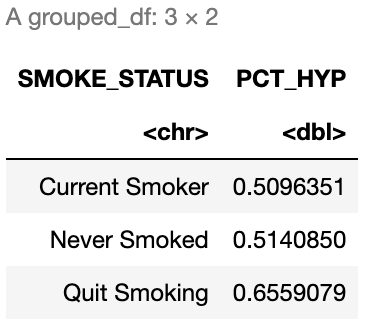
\includegraphics[width=2.08333in,height=\textheight]{book/images/data_transformations_summaries/grouping-and-summarizing.png}

}

\caption{\label{fig-grouping-and-summarizing}Grouping and Summarizing
Data.}

\end{figure}%

\begin{Shaded}
\begin{Highlighting}[]
\CommentTok{\# Insert your solution here:}
\end{Highlighting}
\end{Shaded}

\section{Exercises}\label{exercises-3}

The following exercises use the \texttt{covidcases} dataset
\index{Datasets!covidcases@\texttt{covidcases}} from the
\textbf{HDSinRdata} package\index{R packages!HDSinRdata}. Before
completing the exercises, be sure to read the documentation for this
data (\texttt{?covidcases}).

\begin{Shaded}
\begin{Highlighting}[]
\FunctionTok{data}\NormalTok{(covidcases)}
\end{Highlighting}
\end{Shaded}

\begin{enumerate}
\def\labelenumi{\arabic{enumi}.}
\item
  Suppose we are interested in the distribution of weekly cases by
  state. First, create a new column in \texttt{covidcases} called
  \texttt{region} specifying whether each state is in the Northeast,
  Midwest, South, or West (you can either do this by hand using
  \href{https://en.wikipedia.org/wiki/List_of_regions_of_the_United_States}{this
  list} of which states are in which region, or you can use
  \texttt{state.region} from the \textbf{datasets} package in R). Then,
  create a data frame summarizing the average and standard deviation of
  the weekly cases for the Northeast.
\item
  Now, create a data frame with the average and standard deviation
  summarized for each region rather than for just one selected region as
  in Question 1. Sort this data frame from highest to lowest average
  weekly cases. What other information would you need in order to more
  accurately compare these regions in terms of their average cases?
\item
  Find the ten counties in the Midwest with the lowest weekly deaths in
  week 15 of this data ignoring ties (use \texttt{slice\_min()} to find
  the argument needed for this). What do you notice about the minimum
  values? See the data documentation for why we observe these values.
\item
  Filter the data to include weeks 9 and 20 (around the start of the
  pandemic), get the total cases per county during that time frame, and
  then find the county in each state that had the highest number of
  total cases.
\end{enumerate}

\chapter{Case Study: Cleaning Tuberculosis Screening
Data}\label{sec-cs-preprocessing}

In this chapter, we put some of our R skills together in a case
study\index{Case study:data cleaning and pre-processing}. This case
study focuses on data cleaning and pre-processing. We use the
\texttt{tb\_diagnosis\_raw}\index{R packages!readr}
\index{Datasets!tb\textunderscore diagnosis\textunderscore raw@\texttt{tb\textunderscore diagnosis\textunderscore raw}}
data from the \textbf{HDSinRdata} package\index{R packages!HDSinRdata}.
This data contains information on 1,634 patients in rural South Africa
who presented at a health clinic with tuberculosis-related symptoms and
were tested for tuberculosis (TB) using Xpert MTB/RIF. Our goal is to
clean this data to reflect the pre-processing described in Baik et al.
(2020). This paper uses this data to derive a simple risk score model
for screening patients for treatment while awaiting Xpert results. We
use the \textbf{tidyverse}\index{R packages!tidyverse} packages as well
as the summary tables from
\textbf{gtsummary}\index{R packages!gtsummary}.

\begin{Shaded}
\begin{Highlighting}[]
\FunctionTok{library}\NormalTok{(HDSinRdata)}
\FunctionTok{library}\NormalTok{(tidyverse)}
\FunctionTok{library}\NormalTok{(gt)}
\FunctionTok{library}\NormalTok{(gtsummary)}
\end{Highlighting}
\end{Shaded}

To begin, read in the data and review the description of the original
columns. Some things to note in the data documentation are the ways
unknown, missing, or refused values are coded as well as how some of the
columns are related to each other.

\begin{Shaded}
\begin{Highlighting}[]
\CommentTok{\# Read in data}
\FunctionTok{data}\NormalTok{(}\StringTok{"tb\_diagnosis\_raw"}\NormalTok{)}

\CommentTok{\# Inspect variable descriptions}
\CommentTok{\# ?tb\_diagnosis\_raw}
\end{Highlighting}
\end{Shaded}

To start, we select variables needed for our analysis. In particular, we
drop columns related to the participation in the survey and about
seeking care. Since some of these variables contain long or vague names,
we also rename most of the variables\index{renaming columns}.

\begin{Shaded}
\begin{Highlighting}[]
\CommentTok{\# Select variables and rename}
\NormalTok{tb\_df }\OtherTok{\textless{}{-}}\NormalTok{ tb\_diagnosis\_raw }\SpecialCharTok{\%\textgreater{}\%} 
  \FunctionTok{select}\NormalTok{(}\FunctionTok{c}\NormalTok{(xpert\_status\_fac, age\_group, sex, hiv\_status\_fac,}
\NormalTok{           other\_conditions\_fac\_\_\_1, other\_conditions\_fac\_\_\_3,}
\NormalTok{           other\_conditions\_fac\_\_\_88, other\_conditions\_fac\_\_\_99,}
\NormalTok{           symp\_fac\_\_\_1, symp\_fac\_\_\_2, symp\_fac\_\_\_3, symp\_fac\_\_\_4, }
\NormalTok{           symp\_fac\_\_\_99, length\_symp\_unit\_fac, length\_symp\_days\_fac,}
\NormalTok{           length\_symp\_wk\_fac, length\_symp\_mnt\_fac, length\_symp\_yr\_fac,}
\NormalTok{           smk\_fac, dx\_tb\_past\_fac, educ\_fac)) }\SpecialCharTok{\%\textgreater{}\%}
    \FunctionTok{rename}\NormalTok{(}\AttributeTok{tb =}\NormalTok{ xpert\_status\_fac, }\AttributeTok{hiv\_pos =}\NormalTok{ hiv\_status\_fac,}
           \AttributeTok{cough =}\NormalTok{ symp\_fac\_\_\_1, }\AttributeTok{fever =}\NormalTok{ symp\_fac\_\_\_2, }
           \AttributeTok{weight\_loss =}\NormalTok{ symp\_fac\_\_\_3, }\AttributeTok{night\_sweats =}\NormalTok{ symp\_fac\_\_\_4, }
           \AttributeTok{symptoms\_missing =}\NormalTok{ symp\_fac\_\_\_99,}
           \AttributeTok{ever\_smoke =}\NormalTok{ smk\_fac, }
           \AttributeTok{past\_tb =}\NormalTok{ dx\_tb\_past\_fac, }\AttributeTok{education =}\NormalTok{ educ\_fac)}
\end{Highlighting}
\end{Shaded}

We then use a summary table \index{tables!summary table} to understand
the initial distributions of the variables observed. This also
highlights where we have missing or unknown data.

\begin{Shaded}
\begin{Highlighting}[]
\FunctionTok{tbl\_summary}\NormalTok{(tb\_df) }\SpecialCharTok{\%\textgreater{}\%}
  \FunctionTok{as\_gt}\NormalTok{()}
\end{Highlighting}
\end{Shaded}

\setlength{\LTpost}{0mm}
\begin{longtable*}{lc}
\toprule
\textbf{Characteristic} & \textbf{N = 1,634}\textsuperscript{\textit{1}} \\ 
\midrule\addlinespace[2.5pt]
tb &  \\ 
    1 & 765 (47\%) \\ 
    2 & 869 (53\%) \\ 
age\_group &  \\ 
    [15,25) & 240 (15\%) \\ 
    [25,35) & 333 (20\%) \\ 
    [35,45) & 385 (24\%) \\ 
    [45,55) & 343 (21\%) \\ 
    [55,99) & 333 (20\%) \\ 
sex &  \\ 
    1 & 830 (51\%) \\ 
    2 & 804 (49\%) \\ 
hiv\_pos &  \\ 
    1 & 632 (39\%) \\ 
    2 & 815 (50\%) \\ 
    77 & 139 (8.5\%) \\ 
    88 & 48 (2.9\%) \\ 
other\_conditions\_fac\_\_\_1 & 895 (55\%) \\ 
other\_conditions\_fac\_\_\_3 & 52 (3.2\%) \\ 
other\_conditions\_fac\_\_\_88 & 11 (0.7\%) \\ 
other\_conditions\_fac\_\_\_99 & 30 (1.8\%) \\ 
cough & 1,279 (78\%) \\ 
fever & 479 (29\%) \\ 
weight\_loss & 534 (33\%) \\ 
night\_sweats & 579 (35\%) \\ 
symptoms\_missing & 22 (1.3\%) \\ 
length\_symp\_unit\_fac &  \\ 
    1 & 207 (14\%) \\ 
    2 & 603 (39\%) \\ 
    3 & 538 (35\%) \\ 
    4 & 83 (5.4\%) \\ 
    77 & 98 (6.4\%) \\ 
    Unknown & 105 \\ 
length\_symp\_days\_fac & 3 (3, 4) \\ 
    Unknown & 1,427 \\ 
length\_symp\_wk\_fac &  \\ 
    1 & 183 (30\%) \\ 
    2 & 237 (39\%) \\ 
    3 & 147 (24\%) \\ 
    4 & 15 (2.5\%) \\ 
    5 & 5 (0.8\%) \\ 
    6 & 13 (2.2\%) \\ 
    7 & 3 (0.5\%) \\ 
    Unknown & 1,031 \\ 
length\_symp\_mnt\_fac & 2 (1, 3) \\ 
    Unknown & 1,096 \\ 
length\_symp\_yr\_fac & 2 (1, 4) \\ 
    Unknown & 1,551 \\ 
ever\_smoke &  \\ 
    1 & 294 (18\%) \\ 
    2 & 252 (15\%) \\ 
    3 & 1,072 (66\%) \\ 
    99 & 16 (1.0\%) \\ 
past\_tb &  \\ 
    1 & 255 (16\%) \\ 
    2 & 1,354 (83\%) \\ 
    77 & 25 (1.5\%) \\ 
education & 10 (7, 12) \\ 
\bottomrule
\end{longtable*}
\begin{minipage}{\linewidth}
\textsuperscript{\textit{1}}n (\%); Median (IQR)\\
\end{minipage}

One observation from the table is that the coding of variables is
inconsistent, with some using 0/1 and others using 1/2. We want to
standardize how these variables are represented\index{re-coding}. To
start, we update our \texttt{tb} column. Additionally, we create a
column \texttt{male} from the previous column \texttt{sex} to make the
reference level clear. We can then drop the \texttt{sex} column.

\begin{Shaded}
\begin{Highlighting}[]
\CommentTok{\# Re{-}code binary variables to 0/1 instead of 1/2}
\NormalTok{tb\_df}\SpecialCharTok{$}\NormalTok{tb }\OtherTok{\textless{}{-}} \FunctionTok{case\_when}\NormalTok{(tb\_df}\SpecialCharTok{$}\NormalTok{tb }\SpecialCharTok{==} \DecValTok{1} \SpecialCharTok{\textasciitilde{}} \StringTok{"TB Positive"}\NormalTok{, }
\NormalTok{                      tb\_df}\SpecialCharTok{$}\NormalTok{tb }\SpecialCharTok{==} \DecValTok{2} \SpecialCharTok{\textasciitilde{}} \StringTok{"TB Negative"}\NormalTok{)}

\NormalTok{tb\_df}\SpecialCharTok{$}\NormalTok{male }\OtherTok{\textless{}{-}} \FunctionTok{case\_when}\NormalTok{(tb\_df}\SpecialCharTok{$}\NormalTok{sex }\SpecialCharTok{==} \DecValTok{1} \SpecialCharTok{\textasciitilde{}} \DecValTok{1}\NormalTok{, }
\NormalTok{                        tb\_df}\SpecialCharTok{$}\NormalTok{sex }\SpecialCharTok{==} \DecValTok{2} \SpecialCharTok{\textasciitilde{}} \DecValTok{0}\NormalTok{)}
\NormalTok{tb\_df }\OtherTok{\textless{}{-}}\NormalTok{ tb\_df }\SpecialCharTok{\%\textgreater{}\%} \FunctionTok{select}\NormalTok{(}\SpecialCharTok{{-}}\FunctionTok{c}\NormalTok{(sex))}
\end{Highlighting}
\end{Shaded}

Diabetes is another variable that should be coded this way. In the raw
data, several columns correspond to this question about other medical
conditions. Therefore, we need to use the columns
\texttt{other\_conditions\_fac\_\_\_88} and
\texttt{other\_conditions\_fac\_\_\_99} to check whether the participant
did not answer the question when interpreting the 0/1 value for
diabetes.

\begin{Shaded}
\begin{Highlighting}[]
\CommentTok{\# Re{-}code diabetes to check if missing}
\NormalTok{tb\_df}\SpecialCharTok{$}\NormalTok{diabetes }\OtherTok{\textless{}{-}} \FunctionTok{case\_when}\NormalTok{(tb\_df}\SpecialCharTok{$}\NormalTok{other\_conditions\_fac\_\_\_3 }\SpecialCharTok{==} \DecValTok{1} \SpecialCharTok{\textasciitilde{}} \DecValTok{1}\NormalTok{,}
\NormalTok{                            tb\_df}\SpecialCharTok{$}\NormalTok{other\_conditions\_fac\_\_\_1 }\SpecialCharTok{==} \DecValTok{1} \SpecialCharTok{\textasciitilde{}} \DecValTok{0}\NormalTok{,}
\NormalTok{                            tb\_df}\SpecialCharTok{$}\NormalTok{other\_conditions\_fac\_\_\_88 }\SpecialCharTok{==} \DecValTok{1} \SpecialCharTok{\textasciitilde{}} \ConstantTok{NA}\NormalTok{,}
\NormalTok{                            tb\_df}\SpecialCharTok{$}\NormalTok{other\_conditions\_fac\_\_\_99 }\SpecialCharTok{==} \DecValTok{1} \SpecialCharTok{\textasciitilde{}} \ConstantTok{NA}\NormalTok{,}
                            \ConstantTok{TRUE} \SpecialCharTok{\textasciitilde{}} \DecValTok{0}\NormalTok{)}
\NormalTok{tb\_df }\OtherTok{\textless{}{-}}\NormalTok{ tb\_df }\SpecialCharTok{\%\textgreater{}\%} \FunctionTok{select}\NormalTok{(}\SpecialCharTok{{-}}\FunctionTok{c}\NormalTok{(other\_conditions\_fac\_\_\_1,}
\NormalTok{                             other\_conditions\_fac\_\_\_3,}
\NormalTok{                             other\_conditions\_fac\_\_\_88,}
\NormalTok{                             other\_conditions\_fac\_\_\_99))}
\FunctionTok{table}\NormalTok{(tb\_df}\SpecialCharTok{$}\NormalTok{diabetes)}
\CommentTok{\#\textgreater{} }
\CommentTok{\#\textgreater{}    0    1 }
\CommentTok{\#\textgreater{} 1541   52}
\end{Highlighting}
\end{Shaded}

Next, we similarly code our variables about HIV status, smoking, and
whether the patient has ever been diagnosed with tuberculosis before.
For these variables, if the patient answered that they did not know
their HIV status or if they had tested positive for TB, we code these as
0 to be consistent with the paper.

\begin{Shaded}
\begin{Highlighting}[]
\CommentTok{\# Re{-}code variables with missing or refused values}
\NormalTok{tb\_df}\SpecialCharTok{$}\NormalTok{hiv\_pos }\OtherTok{\textless{}{-}} \FunctionTok{case\_when}\NormalTok{((tb\_df}\SpecialCharTok{$}\NormalTok{hiv\_pos }\SpecialCharTok{==} \DecValTok{1}\NormalTok{) }\SpecialCharTok{\textasciitilde{}} \DecValTok{1}\NormalTok{, }
\NormalTok{                           tb\_df}\SpecialCharTok{$}\NormalTok{hiv\_pos }\SpecialCharTok{\%in\%} \FunctionTok{c}\NormalTok{(}\DecValTok{2}\NormalTok{,}\DecValTok{77}\NormalTok{) }\SpecialCharTok{\textasciitilde{}} \DecValTok{0}\NormalTok{,}
\NormalTok{                           tb\_df}\SpecialCharTok{$}\NormalTok{hiv\_pos }\SpecialCharTok{==} \DecValTok{88} \SpecialCharTok{\textasciitilde{}} \ConstantTok{NA}\NormalTok{)}

\NormalTok{tb\_df}\SpecialCharTok{$}\NormalTok{ever\_smoke }\OtherTok{\textless{}{-}} \FunctionTok{case\_when}\NormalTok{(tb\_df}\SpecialCharTok{$}\NormalTok{ever\_smoke }\SpecialCharTok{\%in\%} \FunctionTok{c}\NormalTok{(}\DecValTok{1}\NormalTok{,}\DecValTok{2}\NormalTok{) }\SpecialCharTok{\textasciitilde{}} \DecValTok{1}\NormalTok{,}
\NormalTok{                              tb\_df}\SpecialCharTok{$}\NormalTok{ever\_smoke }\SpecialCharTok{==} \DecValTok{3} \SpecialCharTok{\textasciitilde{}} \DecValTok{0}\NormalTok{,}
\NormalTok{                              tb\_df}\SpecialCharTok{$}\NormalTok{ever\_smoke }\SpecialCharTok{==} \DecValTok{99} \SpecialCharTok{\textasciitilde{}} \ConstantTok{NA}\NormalTok{)}

\NormalTok{tb\_df}\SpecialCharTok{$}\NormalTok{past\_tb }\OtherTok{\textless{}{-}} \FunctionTok{case\_when}\NormalTok{(tb\_df}\SpecialCharTok{$}\NormalTok{past\_tb }\SpecialCharTok{==} \DecValTok{1} \SpecialCharTok{\textasciitilde{}} \DecValTok{1}\NormalTok{, }
\NormalTok{                           tb\_df}\SpecialCharTok{$}\NormalTok{past\_tb }\SpecialCharTok{\%in\%} \FunctionTok{c}\NormalTok{(}\DecValTok{2}\NormalTok{,}\DecValTok{77}\NormalTok{) }\SpecialCharTok{\textasciitilde{}} \DecValTok{0}\NormalTok{)}
\end{Highlighting}
\end{Shaded}

The next variable we clean is \texttt{education}. First, we need to code
NA values correctly. We can then observe the distribution of years of
education.

\begin{Shaded}
\begin{Highlighting}[]
\CommentTok{\# Code NA values and look at education distribution}
\NormalTok{tb\_df}\SpecialCharTok{$}\NormalTok{education[tb\_df}\SpecialCharTok{$}\NormalTok{education }\SpecialCharTok{==} \DecValTok{99}\NormalTok{] }\OtherTok{\textless{}{-}} \ConstantTok{NA}
\FunctionTok{hist}\NormalTok{(tb\_df}\SpecialCharTok{$}\NormalTok{education, }\AttributeTok{xlab =} \StringTok{"Years of Education"}\NormalTok{, }
     \AttributeTok{main =} \StringTok{"Histogram of Education Years"}\NormalTok{)}
\end{Highlighting}
\end{Shaded}

\begin{center}
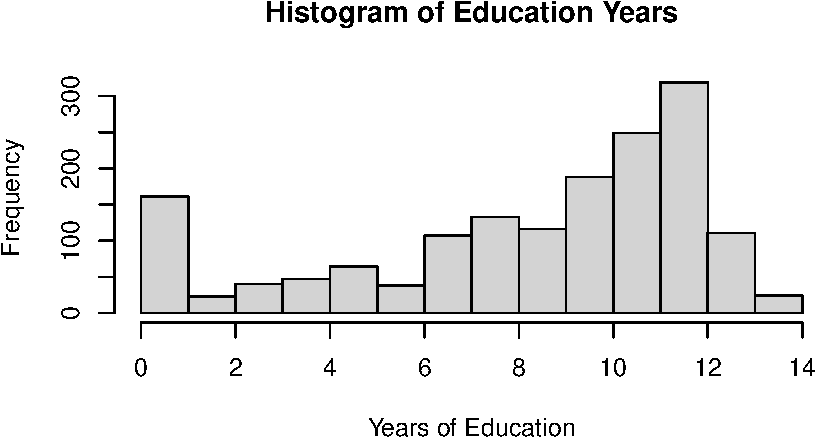
\includegraphics[width=1\textwidth,height=\textheight]{book/cs_preprocessing_files/figure-pdf/unnamed-chunk-8-1.pdf}
\end{center}

For our purposes, we want to represent education as whether a person has
a high school education or less.

\begin{Shaded}
\begin{Highlighting}[]
\CommentTok{\# Categorize education to HS and above}
\NormalTok{tb\_df}\SpecialCharTok{$}\NormalTok{hs\_less }\OtherTok{\textless{}{-}} \FunctionTok{case\_when}\NormalTok{(tb\_df}\SpecialCharTok{$}\NormalTok{education }\SpecialCharTok{\textless{}=} \DecValTok{12} \SpecialCharTok{\textasciitilde{}} \DecValTok{1}\NormalTok{,}
\NormalTok{                           tb\_df}\SpecialCharTok{$}\NormalTok{education }\SpecialCharTok{\textgreater{}} \DecValTok{12} \SpecialCharTok{\textasciitilde{}} \DecValTok{0}\NormalTok{,}
                           \ConstantTok{TRUE} \SpecialCharTok{\textasciitilde{}} \ConstantTok{NA}\NormalTok{)}
\NormalTok{tb\_df }\OtherTok{\textless{}{-}}\NormalTok{ tb\_df }\SpecialCharTok{\%\textgreater{}\%} \FunctionTok{select}\NormalTok{(}\SpecialCharTok{{-}}\FunctionTok{c}\NormalTok{(education))}
\end{Highlighting}
\end{Shaded}

There are several variables in the data related to how long a person has
experienced symptoms. In the following code, we can see that the unit of
the symptoms, recorded in \texttt{length\_symp\_unit\_fac}, determines
which other column is entered. For example, if
\texttt{length\_symp\_unit\_fac\ ==\ 1}, then the only column without an
NA value is \texttt{length\_symp\_days\_fc}.

\begin{Shaded}
\begin{Highlighting}[]
\NormalTok{tb\_df }\SpecialCharTok{\%\textgreater{}\%}
  \FunctionTok{group\_by}\NormalTok{(length\_symp\_unit\_fac) }\SpecialCharTok{\%\textgreater{}\%}
  \FunctionTok{summarize}\NormalTok{(}\AttributeTok{missing\_days =} \FunctionTok{sum}\NormalTok{(}\FunctionTok{is.na}\NormalTok{(length\_symp\_days\_fac))}\SpecialCharTok{/}\FunctionTok{n}\NormalTok{(),}
            \AttributeTok{missing\_wks =} \FunctionTok{sum}\NormalTok{(}\FunctionTok{is.na}\NormalTok{(length\_symp\_wk\_fac))}\SpecialCharTok{/}\FunctionTok{n}\NormalTok{(),}
            \AttributeTok{missing\_mnt =} \FunctionTok{sum}\NormalTok{(}\FunctionTok{is.na}\NormalTok{(length\_symp\_mnt\_fac))}\SpecialCharTok{/}\FunctionTok{n}\NormalTok{(),}
            \AttributeTok{missing\_yr =} \FunctionTok{sum}\NormalTok{(}\FunctionTok{is.na}\NormalTok{(length\_symp\_yr\_fac))}\SpecialCharTok{/}\FunctionTok{n}\NormalTok{())}
\CommentTok{\#\textgreater{} \# A tibble: 6 x 5}
\CommentTok{\#\textgreater{}   length\_symp\_unit\_fac missing\_days missing\_wks missing\_mnt missing\_yr}
\CommentTok{\#\textgreater{}                  \textless{}int\textgreater{}        \textless{}dbl\textgreater{}       \textless{}dbl\textgreater{}       \textless{}dbl\textgreater{}      \textless{}dbl\textgreater{}}
\CommentTok{\#\textgreater{} 1                    1            0           1           1          1}
\CommentTok{\#\textgreater{} 2                    2            1           0           1          1}
\CommentTok{\#\textgreater{} 3                    3            1           1           0          1}
\CommentTok{\#\textgreater{} 4                    4            1           1           1          0}
\CommentTok{\#\textgreater{} 5                   77            1           1           1          1}
\CommentTok{\#\textgreater{} 6                   NA            1           1           1          1}
\end{Highlighting}
\end{Shaded}

Additionally, these measurements are positive integer values.

\begin{Shaded}
\begin{Highlighting}[]
\FunctionTok{min}\NormalTok{(tb\_df}\SpecialCharTok{$}\NormalTok{length\_symp\_days\_fac, }\AttributeTok{na.rm =} \ConstantTok{TRUE}\NormalTok{)}
\CommentTok{\#\textgreater{} [1] 1}
\FunctionTok{is.integer}\NormalTok{(tb\_df}\SpecialCharTok{$}\NormalTok{length\_symp\_days\_fac)}
\CommentTok{\#\textgreater{} [1] TRUE}
\end{Highlighting}
\end{Shaded}

This allows us to create a new variable that represents whether or not
someone has had symptoms for more than two weeks. In our
\texttt{case\_when()}\index{R functions!case\textunderscore when()@\texttt{case\textunderscore when()}}
function call, we first check whether the duration is missing before
checking for the cases when symptoms would be less than two weeks.

\begin{Shaded}
\begin{Highlighting}[]
\CommentTok{\# Categorize number of weeks experiencing symptoms}
\NormalTok{tb\_df }\OtherTok{\textless{}{-}}\NormalTok{ tb\_df }\SpecialCharTok{\%\textgreater{}\%}
  \FunctionTok{mutate}\NormalTok{(}\AttributeTok{two\_weeks =} \FunctionTok{case\_when}\NormalTok{((length\_symp\_unit\_fac }\SpecialCharTok{==} \DecValTok{77} \SpecialCharTok{|}
                      \FunctionTok{is.na}\NormalTok{(length\_symp\_unit\_fac)) }\SpecialCharTok{\textasciitilde{}} \ConstantTok{NA}\NormalTok{,}
\NormalTok{                   (length\_symp\_unit\_fac }\SpecialCharTok{==} \DecValTok{1} \SpecialCharTok{\&} 
\NormalTok{                      length\_symp\_days\_fac }\SpecialCharTok{\textless{}=} \DecValTok{14}\NormalTok{) }\SpecialCharTok{\textasciitilde{}} \DecValTok{0}\NormalTok{,}
\NormalTok{                   (length\_symp\_unit\_fac }\SpecialCharTok{==} \DecValTok{2} \SpecialCharTok{\&}
\NormalTok{                      length\_symp\_wk\_fac }\SpecialCharTok{\textless{}=} \DecValTok{2}\NormalTok{) }\SpecialCharTok{\textasciitilde{}} \DecValTok{0}\NormalTok{,}
                   \ConstantTok{TRUE} \SpecialCharTok{\textasciitilde{}} \DecValTok{1}\NormalTok{))}

\NormalTok{tb\_df }\OtherTok{\textless{}{-}}\NormalTok{ tb\_df }\SpecialCharTok{\%\textgreater{}\%} 
  \FunctionTok{select}\NormalTok{(}\SpecialCharTok{{-}}\FunctionTok{c}\NormalTok{(length\_symp\_wk\_fac, length\_symp\_days\_fac, }
\NormalTok{            length\_symp\_mnt\_fac, length\_symp\_yr\_fac, }
\NormalTok{            length\_symp\_unit\_fac))}
\end{Highlighting}
\end{Shaded}

Last, we update our symptom variables to have a summary column
\texttt{num\_symptoms} that represents the total number of classic TB
symptoms rather than keeping track of individual symptoms. We also
exclude anyone who does not have any TB symptoms.

\begin{Shaded}
\begin{Highlighting}[]
\CommentTok{\# Count total number of symptoms}
\NormalTok{tb\_df}\SpecialCharTok{$}\NormalTok{num\_symptoms }\OtherTok{\textless{}{-}}\NormalTok{ tb\_df}\SpecialCharTok{$}\NormalTok{fever }\SpecialCharTok{+}\NormalTok{ tb\_df}\SpecialCharTok{$}\NormalTok{weight\_loss }\SpecialCharTok{+}\NormalTok{ tb\_df}\SpecialCharTok{$}\NormalTok{cough }\SpecialCharTok{+} 
\NormalTok{  tb\_df}\SpecialCharTok{$}\NormalTok{night\_sweats}
\NormalTok{tb\_df}\SpecialCharTok{$}\NormalTok{num\_symptoms[tb\_df}\SpecialCharTok{$}\NormalTok{symptoms\_missing }\SpecialCharTok{==} \DecValTok{1}\NormalTok{] }\OtherTok{\textless{}{-}} \ConstantTok{NA}
\NormalTok{tb\_df }\OtherTok{\textless{}{-}}\NormalTok{ tb\_df }\SpecialCharTok{\%\textgreater{}\%} \FunctionTok{select}\NormalTok{(}\SpecialCharTok{{-}}\FunctionTok{c}\NormalTok{(night\_sweats, weight\_loss, cough, fever,}
\NormalTok{                             symptoms\_missing))}

\CommentTok{\# Exclude observations with no TB symptoms }
\NormalTok{tb\_df }\OtherTok{\textless{}{-}}\NormalTok{ tb\_df }\SpecialCharTok{\%\textgreater{}\%}
  \FunctionTok{filter}\NormalTok{(num\_symptoms }\SpecialCharTok{!=} \DecValTok{0}\NormalTok{)}

\FunctionTok{table}\NormalTok{(tb\_df}\SpecialCharTok{$}\NormalTok{num\_symptoms)}
\CommentTok{\#\textgreater{} }
\CommentTok{\#\textgreater{}   1   2   3   4 }
\CommentTok{\#\textgreater{} 600 344 265 196}
\end{Highlighting}
\end{Shaded}

Last, we convert all variables to factors.

\begin{Shaded}
\begin{Highlighting}[]
\CommentTok{\# Convert all variables to factors }
\NormalTok{tb\_df[] }\OtherTok{\textless{}{-}} \FunctionTok{lapply}\NormalTok{(tb\_df, }\ControlFlowTok{function}\NormalTok{(x)\{}\FunctionTok{return}\NormalTok{(}\FunctionTok{as.factor}\NormalTok{(x))\})}
\end{Highlighting}
\end{Shaded}

Our final data is summarized in the following table. The
\texttt{add\_overall()}\index{R functions!add\textunderscore overall()@\texttt{add\textunderscore overall()}}
function includes the overall summary statistics in addition to our
stratified summaries. Our summary table looks similar to the one in the
paper. However, it looks like we have a few more observations included.
Additionally, our education variable shows a lower percentage of
observations with post-high school education and positive HIV status.

\begin{Shaded}
\begin{Highlighting}[]
\FunctionTok{tbl\_summary}\NormalTok{(tb\_df, }\AttributeTok{by =} \StringTok{"tb"}\NormalTok{,}
            \AttributeTok{label =} \FunctionTok{list}\NormalTok{(}
              \AttributeTok{tb=} \StringTok{"Tuberculosis"}\NormalTok{,}
              \AttributeTok{age\_group =} \StringTok{"Age Group"}\NormalTok{,}
              \AttributeTok{hiv\_pos =} \StringTok{"HIV Positive"}\NormalTok{,}
              \AttributeTok{ever\_smoke =} \StringTok{"Ever Smoked"}\NormalTok{,}
              \AttributeTok{past\_tb =} \StringTok{"Past TB"}\NormalTok{,}
              \AttributeTok{male =} \StringTok{"Male"}\NormalTok{,}
              \AttributeTok{hs\_less =} \StringTok{"High School or Less Educ."}\NormalTok{,}
              \AttributeTok{two\_weeks =} \StringTok{"Two Weeks Symptoms"}\NormalTok{,}
              \AttributeTok{diabetes =} \StringTok{"Diabetes"}\NormalTok{,}
              \AttributeTok{num\_symptoms =} \StringTok{"Number of Symptoms"}
\NormalTok{            )) }\SpecialCharTok{\%\textgreater{}\%}
  \FunctionTok{add\_overall}\NormalTok{() }\SpecialCharTok{\%\textgreater{}\%}
  \FunctionTok{as\_gt}\NormalTok{() }\SpecialCharTok{\%\textgreater{}\%}
  \FunctionTok{cols\_width}\NormalTok{(}\FunctionTok{everything}\NormalTok{() }\SpecialCharTok{\textasciitilde{}} \StringTok{"55pt"}\NormalTok{)}
\end{Highlighting}
\end{Shaded}

\setlength{\LTpost}{0mm}
\begin{longtable*}{>{\raggedright\arraybackslash}p{55pt}>{\centering\arraybackslash}p{55pt}>{\centering\arraybackslash}p{55pt}>{\centering\arraybackslash}p{55pt}}
\toprule
\textbf{Characteristic} & \textbf{Overall}, N = 1,405\textsuperscript{\textit{1}} & \textbf{TB Negative}, N = 704\textsuperscript{\textit{1}} & \textbf{TB Positive}, N = 701\textsuperscript{\textit{1}} \\ 
\midrule\addlinespace[2.5pt]
Age Group &  &  &  \\ 
    [15,25) & 205 (15\%) & 121 (17\%) & 84 (12\%) \\ 
    [25,35) & 286 (20\%) & 120 (17\%) & 166 (24\%) \\ 
    [35,45) & 338 (24\%) & 136 (19\%) & 202 (29\%) \\ 
    [45,55) & 305 (22\%) & 158 (22\%) & 147 (21\%) \\ 
    [55,99) & 271 (19\%) & 169 (24\%) & 102 (15\%) \\ 
HIV Positive &  &  &  \\ 
    0 & 808 (59\%) & 503 (73\%) & 305 (45\%) \\ 
    1 & 556 (41\%) & 186 (27\%) & 370 (55\%) \\ 
    Unknown & 41 & 15 & 26 \\ 
Ever Smoked &  &  &  \\ 
    0 & 899 (64\%) & 483 (69\%) & 416 (60\%) \\ 
    1 & 496 (36\%) & 213 (31\%) & 283 (40\%) \\ 
    Unknown & 10 & 8 & 2 \\ 
Past TB &  &  &  \\ 
    0 & 1,186 (84\%) & 613 (87\%) & 573 (82\%) \\ 
    1 & 219 (16\%) & 91 (13\%) & 128 (18\%) \\ 
Male &  &  &  \\ 
    0 & 669 (48\%) & 394 (56\%) & 275 (39\%) \\ 
    1 & 736 (52\%) & 310 (44\%) & 426 (61\%) \\ 
Diabetes &  &  &  \\ 
    0 & 1,326 (97\%) & 658 (97\%) & 668 (96\%) \\ 
    1 & 47 (3.4\%) & 22 (3.2\%) & 25 (3.6\%) \\ 
    Unknown & 32 & 24 & 8 \\ 
High School or Less Educ. &  &  &  \\ 
    0 & 119 (8.5\%) & 73 (10\%) & 46 (6.6\%) \\ 
    1 & 1,276 (91\%) & 625 (90\%) & 651 (93\%) \\ 
    Unknown & 10 & 6 & 4 \\ 
Two Weeks Symptoms &  &  &  \\ 
    0 & 592 (44\%) & 386 (57\%) & 206 (31\%) \\ 
    1 & 760 (56\%) & 294 (43\%) & 466 (69\%) \\ 
    Unknown & 53 & 24 & 29 \\ 
Number of Symptoms &  &  &  \\ 
    1 & 600 (43\%) & 426 (61\%) & 174 (25\%) \\ 
    2 & 344 (24\%) & 181 (26\%) & 163 (23\%) \\ 
    3 & 265 (19\%) & 67 (9.5\%) & 198 (28\%) \\ 
    4 & 196 (14\%) & 30 (4.3\%) & 166 (24\%) \\ 
\bottomrule
\end{longtable*}
\begin{minipage}{\linewidth}
\textsuperscript{\textit{1}}n (\%)\\
\end{minipage}

\chapter{Merging and Reshaping Data}\label{sec-merging-reshaping}

In this chapter, we continue to look at some of the ways to manipulate
data using the \textbf{tidyr}\index{R packages!tidyr} and
\textbf{dplyr}\index{R packages!dplyr} packages, which are part of the
\textbf{tidyverse} group of packages\index{R packages!tidyverse}. In
particular, we look at reshaping and merging data frames in order to get
the data in the format we want. When reshaping data, we can convert
between \emph{wide form}\index{wide form} (more columns, fewer rows) and
\emph{long form}\index{long form} (fewer columns, more rows). We can
also use data pivots to put our data into what is called \emph{tidy
form}\index{tidy data}. Additionally, we look at combining information
from multiple data frames into a single data frame. The key ideas when
merging data are to think about what the common information is between
the data frames and to consider which values we want to keep.

For this chapter, we use three datasets. The first dataset is
\texttt{covidcases}\index{Datasets!covidcases@\texttt{covidcases}},
which contains the weekly COVID-19 case and death counts by county in
the United States for 2020 (Guidotti and Ardia 2020; Guidotti 2022); the
second dataset is
\texttt{mobility}\index{Datasets!mobility@\texttt{mobility}}, which
contains daily mobility estimates by state in 2020 (Warren and Skillman
2020); and the third dataset is
\texttt{lockdowndates}\index{Datasets!lockdowndates@\texttt{lockdowndates}},
which contains the start and end dates for statewide stay-at-home orders
(Raifman et al. 2022). Take a look at the first few rows of each data
frame and read the documentation for the column descriptions.

\begin{Shaded}
\begin{Highlighting}[]
\FunctionTok{library}\NormalTok{(tidyverse)}
\FunctionTok{library}\NormalTok{(HDSinRdata)}

\FunctionTok{data}\NormalTok{(covidcases)}
\FunctionTok{data}\NormalTok{(lockdowndates)}
\FunctionTok{data}\NormalTok{(mobility)}
\end{Highlighting}
\end{Shaded}

\begin{Shaded}
\begin{Highlighting}[]
\FunctionTok{head}\NormalTok{(covidcases)}
\CommentTok{\#\textgreater{} \# A tibble: 6 x 5}
\CommentTok{\#\textgreater{}   state         county   week weekly\_cases weekly\_deaths}
\CommentTok{\#\textgreater{}   \textless{}chr\textgreater{}         \textless{}chr\textgreater{}   \textless{}dbl\textgreater{}        \textless{}int\textgreater{}         \textless{}int\textgreater{}}
\CommentTok{\#\textgreater{} 1 California    Marin       9            1             0}
\CommentTok{\#\textgreater{} 2 California    Orange      9            3             0}
\CommentTok{\#\textgreater{} 3 Florida       Manatee     9            1             0}
\CommentTok{\#\textgreater{} 4 California    Napa        9            1             0}
\CommentTok{\#\textgreater{} 5 New Hampshire Grafton     9            2             0}
\CommentTok{\#\textgreater{} 6 Washington    Spokane     9            4             0}
\end{Highlighting}
\end{Shaded}

\begin{Shaded}
\begin{Highlighting}[]
\FunctionTok{head}\NormalTok{(mobility)}
\CommentTok{\#\textgreater{} \# A tibble: 6 x 5}
\CommentTok{\#\textgreater{} \# Groups:   state [1]}
\CommentTok{\#\textgreater{}   state   date       samples   m50 m50\_index}
\CommentTok{\#\textgreater{}   \textless{}chr\textgreater{}   \textless{}chr\textgreater{}        \textless{}int\textgreater{} \textless{}dbl\textgreater{}     \textless{}dbl\textgreater{}}
\CommentTok{\#\textgreater{} 1 Alabama 2020{-}03{-}01  267652  10.9      76.9}
\CommentTok{\#\textgreater{} 2 Alabama 2020{-}03{-}02  287264  14.3      98.6}
\CommentTok{\#\textgreater{} 3 Alabama 2020{-}03{-}03  292018  14.2      98.2}
\CommentTok{\#\textgreater{} 4 Alabama 2020{-}03{-}04  298704  13.1      89.7}
\CommentTok{\#\textgreater{} 5 Alabama 2020{-}03{-}05  288218  14.8     102. }
\CommentTok{\#\textgreater{} 6 Alabama 2020{-}03{-}06  282982  17.9     126.}
\end{Highlighting}
\end{Shaded}

\begin{Shaded}
\begin{Highlighting}[]
\FunctionTok{head}\NormalTok{(lockdowndates)}
\CommentTok{\#\textgreater{} \# A tibble: 6 x 3}
\CommentTok{\#\textgreater{}   State      Lockdown\_Start Lockdown\_End}
\CommentTok{\#\textgreater{}   \textless{}chr\textgreater{}      \textless{}chr\textgreater{}          \textless{}chr\textgreater{}       }
\CommentTok{\#\textgreater{} 1 Alabama    2020{-}04{-}04     2020{-}04{-}30  }
\CommentTok{\#\textgreater{} 2 Alaska     2020{-}03{-}28     2020{-}04{-}24  }
\CommentTok{\#\textgreater{} 3 Arizona    2020{-}03{-}31     2020{-}05{-}16  }
\CommentTok{\#\textgreater{} 4 Arkansas   None           None        }
\CommentTok{\#\textgreater{} 5 California 2020{-}03{-}19     2021{-}01{-}25  }
\CommentTok{\#\textgreater{} 6 Colorado   2020{-}03{-}26     2020{-}04{-}27}
\end{Highlighting}
\end{Shaded}

Both the mobility and lockdown data frames contain date columns. Right
now, these columns in both datasets are of the class character, which we
can see in the printed output. We can use the
\texttt{as.Date()}\index{R functions!as.Date()@\texttt{as.Date()}}
function to tell R to treat these columns as dates instead of
characters. When using this function, we need to specify the date format
\index{date format} as an argument so that R knows how to parse this
text to a date. Our format is given as \texttt{\%Y-\%M-\%D}, where the
\texttt{\%Y} stands for the full four-digit year, \texttt{\%M} is a
two-digit month (e.g., January is coded ``01'' vs.~``1''), and
\texttt{\%D} stands for the two-digit day (e.g., the third day is coded
``03'' vs.~``3''). In the following code, we convert the classes of
these columns to dates.

\begin{Shaded}
\begin{Highlighting}[]
\NormalTok{mobility}\SpecialCharTok{$}\NormalTok{date }\OtherTok{\textless{}{-}} \FunctionTok{as.Date}\NormalTok{(mobility}\SpecialCharTok{$}\NormalTok{date, }\AttributeTok{formula =} \StringTok{"\%Y{-}\%M{-}\%D"}\NormalTok{)}
\NormalTok{lockdowndates}\SpecialCharTok{$}\NormalTok{Lockdown\_Start }\OtherTok{\textless{}{-}} \FunctionTok{as.Date}\NormalTok{(lockdowndates}\SpecialCharTok{$}\NormalTok{Lockdown\_Start, }
                                        \AttributeTok{formula =} \StringTok{"\%Y{-}\%M{-}\%D"}\NormalTok{)}
\NormalTok{lockdowndates}\SpecialCharTok{$}\NormalTok{Lockdown\_End }\OtherTok{\textless{}{-}} \FunctionTok{as.Date}\NormalTok{(lockdowndates}\SpecialCharTok{$}\NormalTok{Lockdown\_End, }
                                      \AttributeTok{formula =} \StringTok{"\%Y{-}\%M{-}\%D"}\NormalTok{)}
\FunctionTok{class}\NormalTok{(mobility}\SpecialCharTok{$}\NormalTok{date)}
\CommentTok{\#\textgreater{} [1] "Date"}
\FunctionTok{class}\NormalTok{(lockdowndates}\SpecialCharTok{$}\NormalTok{Lockdown\_Start)}
\CommentTok{\#\textgreater{} [1] "Date"}
\FunctionTok{class}\NormalTok{(lockdowndates}\SpecialCharTok{$}\NormalTok{Lockdown\_End)}
\CommentTok{\#\textgreater{} [1] "Date"}
\end{Highlighting}
\end{Shaded}

After coding these columns as dates, we can access information such as
the day, month, year, or week from them. These functions are all
available in the \textbf{lubridate} package (Spinu, Grolemund, and
Wickham 2023)\index{R packages!lubridate}, which is a package in the
\textbf{tidyverse} that allows us to manipulate dates.

\begin{Shaded}
\begin{Highlighting}[]
\FunctionTok{month}\NormalTok{(mobility}\SpecialCharTok{$}\NormalTok{date[}\DecValTok{1}\NormalTok{])}
\CommentTok{\#\textgreater{} [1] 3}
\FunctionTok{week}\NormalTok{(mobility}\SpecialCharTok{$}\NormalTok{date[}\DecValTok{1}\NormalTok{])}
\CommentTok{\#\textgreater{} [1] 9}
\end{Highlighting}
\end{Shaded}

Next, we add a date column to \texttt{covidcases}. In this case, we need
to use the week number to find the date. Luckily, we can add days,
months, weeks, or years to dates using the
\textbf{lubridate}\index{R packages!lubridate} package. January 1, 2020
was a Wednesday and is counted as the first week; so to find the
corresponding Sunday for each week, we add the recorded week number
minus 1 to December 29, 2019 (the last Sunday before 2020). We show a
simple example of adding one week to this date before doing this
conversion for the entire column.

\begin{Shaded}
\begin{Highlighting}[]
\FunctionTok{as.Date}\NormalTok{(}\StringTok{"2019{-}12{-}29"}\NormalTok{) }\SpecialCharTok{+} \FunctionTok{weeks}\NormalTok{(}\DecValTok{1}\NormalTok{)}
\CommentTok{\#\textgreater{} [1] "2020{-}01{-}05"}
\end{Highlighting}
\end{Shaded}

\begin{Shaded}
\begin{Highlighting}[]
\NormalTok{covidcases}\SpecialCharTok{$}\NormalTok{date }\OtherTok{\textless{}{-}} \FunctionTok{as.Date}\NormalTok{(}\StringTok{"2019{-}12{-}29"}\NormalTok{) }\SpecialCharTok{+} \FunctionTok{weeks}\NormalTok{(covidcases}\SpecialCharTok{$}\NormalTok{week }\SpecialCharTok{{-}} \DecValTok{1}\NormalTok{)}
\FunctionTok{head}\NormalTok{(covidcases)}
\CommentTok{\#\textgreater{} \# A tibble: 6 x 6}
\CommentTok{\#\textgreater{}   state         county   week weekly\_cases weekly\_deaths date      }
\CommentTok{\#\textgreater{}   \textless{}chr\textgreater{}         \textless{}chr\textgreater{}   \textless{}dbl\textgreater{}        \textless{}int\textgreater{}         \textless{}int\textgreater{} \textless{}date\textgreater{}    }
\CommentTok{\#\textgreater{} 1 California    Marin       9            1             0 2020{-}02{-}23}
\CommentTok{\#\textgreater{} 2 California    Orange      9            3             0 2020{-}02{-}23}
\CommentTok{\#\textgreater{} 3 Florida       Manatee     9            1             0 2020{-}02{-}23}
\CommentTok{\#\textgreater{} 4 California    Napa        9            1             0 2020{-}02{-}23}
\CommentTok{\#\textgreater{} 5 New Hampshire Grafton     9            2             0 2020{-}02{-}23}
\CommentTok{\#\textgreater{} 6 Washington    Spokane     9            4             0 2020{-}02{-}23}
\end{Highlighting}
\end{Shaded}

\section{Tidy Data}\label{tidy-data}

The \textbf{tidyverse} is designed around interacting with \textbf{tidy
data} \index{tidy data} with the premise that using data in a tidy
format can streamline our analysis. Data is considered \textbf{tidy} if:

\begin{itemize}
\item
  Each variable is associated with a single column.
\item
  Each observation is associated with a single row.
\item
  Each value has its own cell.
\end{itemize}

Take a look at the sample data which stores information about the
maternal mortality rate for five countries over time (Roser and Ritchie
2013). This data is \emph{not} tidy because the variable for maternity
mortality rate is associated with multiple columns. Every row should
correspond to one class observation.

\begin{Shaded}
\begin{Highlighting}[]
\NormalTok{mat\_mort1 }\OtherTok{\textless{}{-}} \FunctionTok{data.frame}\NormalTok{(}\AttributeTok{country =} \FunctionTok{c}\NormalTok{(}\StringTok{"Turkey"}\NormalTok{, }\StringTok{"United States"}\NormalTok{, }
                                    \StringTok{"Sweden"}\NormalTok{, }\StringTok{"Japan"}\NormalTok{),}
                       \AttributeTok{y2002 =} \FunctionTok{c}\NormalTok{(}\DecValTok{64}\NormalTok{, }\FloatTok{9.9}\NormalTok{, }\FloatTok{4.17}\NormalTok{, }\FloatTok{7.8}\NormalTok{),}
                       \AttributeTok{y2007 =} \FunctionTok{c}\NormalTok{(}\FloatTok{21.9}\NormalTok{, }\FloatTok{12.7}\NormalTok{, }\FloatTok{1.86}\NormalTok{, }\FloatTok{3.6}\NormalTok{),}
                       \AttributeTok{y2012 =} \FunctionTok{c}\NormalTok{(}\FloatTok{15.2}\NormalTok{, }\DecValTok{16}\NormalTok{, }\FloatTok{5.4}\NormalTok{, }\FloatTok{4.8}\NormalTok{))}
\FunctionTok{head}\NormalTok{(mat\_mort1)}
\CommentTok{\#\textgreater{}         country y2002 y2007 y2012}
\CommentTok{\#\textgreater{} 1        Turkey 64.00 21.90  15.2}
\CommentTok{\#\textgreater{} 2 United States  9.90 12.70  16.0}
\CommentTok{\#\textgreater{} 3        Sweden  4.17  1.86   5.4}
\CommentTok{\#\textgreater{} 4         Japan  7.80  3.60   4.8}
\end{Highlighting}
\end{Shaded}

However, we can make this data tidy by creating separate columns for
country, year, and maternity mortality rate as we demonstrate in the
following code. Now every observation is associated with an individual
row.

\begin{Shaded}
\begin{Highlighting}[]
\NormalTok{mat\_mort2 }\OtherTok{\textless{}{-}} \FunctionTok{data.frame}\NormalTok{(}
    \AttributeTok{country =} \FunctionTok{rep}\NormalTok{(}\FunctionTok{c}\NormalTok{(}\StringTok{"Turkey"}\NormalTok{, }\StringTok{"United States"}\NormalTok{, }\StringTok{"Sweden"}\NormalTok{, }\StringTok{"Japan"}\NormalTok{), }\DecValTok{3}\NormalTok{),}
    \AttributeTok{year =} \FunctionTok{c}\NormalTok{(}\FunctionTok{rep}\NormalTok{(}\DecValTok{2002}\NormalTok{, }\DecValTok{4}\NormalTok{), }\FunctionTok{rep}\NormalTok{(}\DecValTok{2007}\NormalTok{, }\DecValTok{4}\NormalTok{), }\FunctionTok{rep}\NormalTok{(}\DecValTok{2012}\NormalTok{, }\DecValTok{4}\NormalTok{)),}
    \AttributeTok{mat\_mort\_rate =} \FunctionTok{c}\NormalTok{(}\FloatTok{64.0}\NormalTok{, }\FloatTok{9.9}\NormalTok{, }\FloatTok{4.17}\NormalTok{, }\FloatTok{7.8}\NormalTok{, }\FloatTok{21.9}\NormalTok{, }\FloatTok{12.7}\NormalTok{, }\FloatTok{1.86}\NormalTok{, }\FloatTok{3.6}\NormalTok{, }
                      \FloatTok{15.2}\NormalTok{, }\DecValTok{16}\NormalTok{, }\FloatTok{5.4}\NormalTok{, }\FloatTok{4.8}\NormalTok{))}
\FunctionTok{head}\NormalTok{(mat\_mort2)}
\CommentTok{\#\textgreater{}         country year mat\_mort\_rate}
\CommentTok{\#\textgreater{} 1        Turkey 2002         64.00}
\CommentTok{\#\textgreater{} 2 United States 2002          9.90}
\CommentTok{\#\textgreater{} 3        Sweden 2002          4.17}
\CommentTok{\#\textgreater{} 4         Japan 2002          7.80}
\CommentTok{\#\textgreater{} 5        Turkey 2007         21.90}
\CommentTok{\#\textgreater{} 6 United States 2007         12.70}
\end{Highlighting}
\end{Shaded}

\section{\texorpdfstring{Reshaping Data \index{pivoting data}
\index{reshaping data}}{Reshaping Data  }}\label{reshaping-data}

The mobility and COVID-19 case data are both already in tidy form: each
observation corresponds to a single row, and every column is a single
variable. We might consider whether the lockdown dates should be
re-formatted to be tidy. Another way to represent this data would be to
have each observation be the start or end of a stay-at-home order.

To reshape our data, we use the
\texttt{pivot\_longer()}\index{R functions!pivot\textunderscore longer()@\texttt{pivot\textunderscore longer()}}
function to change the data from what is called \textbf{wide form}
\index{wide form} to what is called \textbf{long form}\index{long form}.
This kind of pivot\index{data pivots} involves taking a subset of
columns that we want to \emph{gather} into a single column while
increasing the number of rows in the dataset. Before pivoting, we have
to think about which columns we are transforming. The image in
Figure~\ref{fig-pivot-long} shows a picture of some data on whether
students have completed a physical, hearing, or eye exam. The data is
presented in wide form on the left and long form on the right. To
transform wide data to long data, we have identified a subset of columns
\texttt{cols} that we want to transform (these \texttt{cols} are
\texttt{phys}, \texttt{hear}, and \texttt{eye} in the left table). The
long form contains a new column \texttt{names\_to} that contains the
exam type, and \texttt{values\_to} that contains a binary variable
indicating whether or not each exam was completed.

\begin{figure}

\centering{

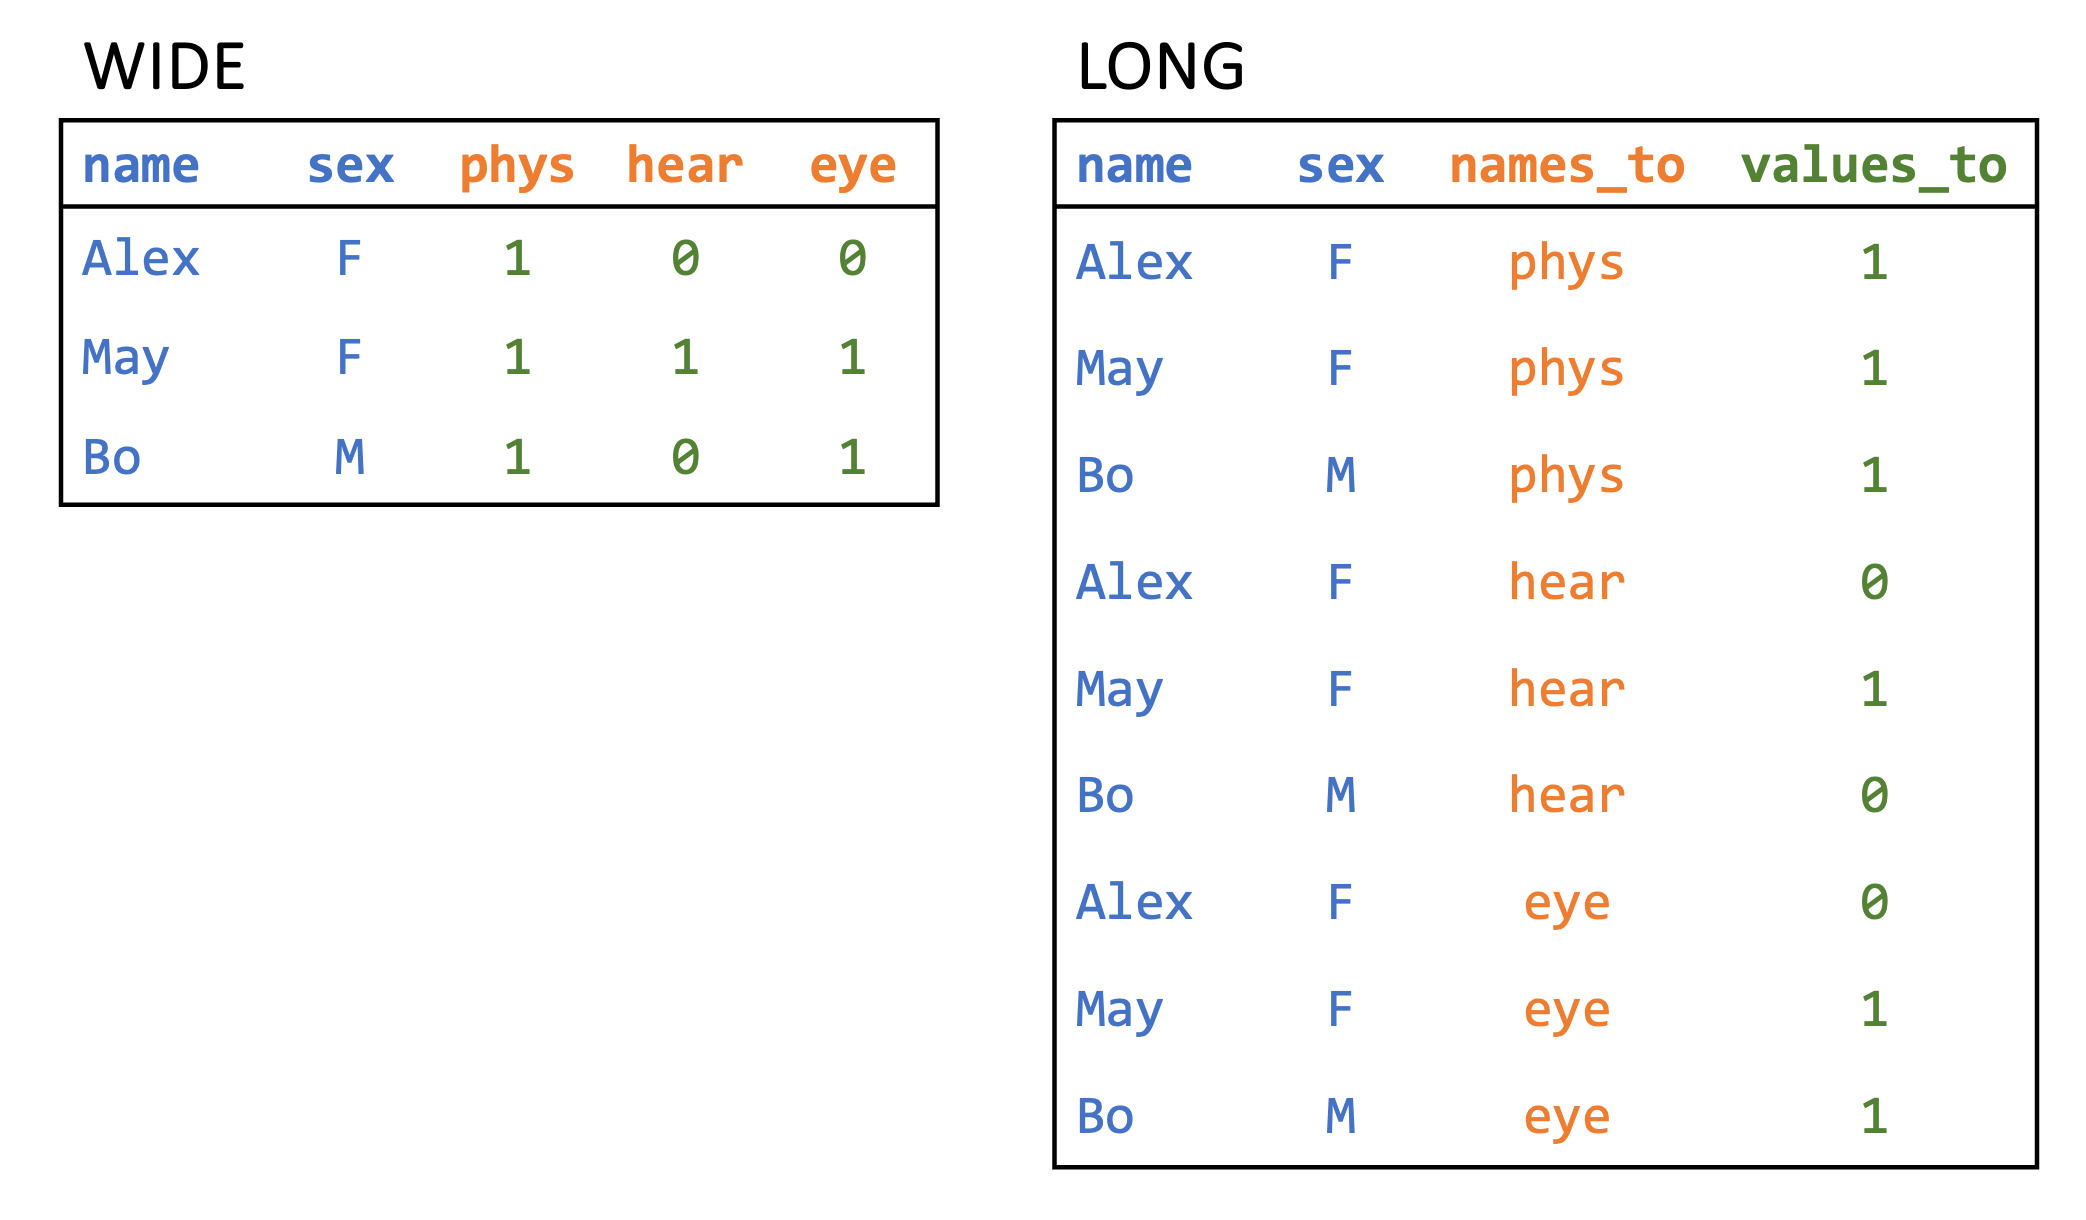
\includegraphics[width=4.16667in,height=\textheight]{book/images/merging_data/pivot-long.png}

}

\caption{\label{fig-pivot-long}Pivoting Longer.}

\end{figure}%

In our case, we want to take the lockdown start and end columns and
create two new columns: one column will indicate whether or not a date
represents the start or end of a lockdown, and the other will contain
the date itself. These are called the \emph{key} and \emph{value}
columns, respectively. The key column gets its values from the names of
the columns we are transforming (or the keys), whereas the value column
gets its values from the entries in those columns (or the values).

The \texttt{pivot\_longer()} function takes in a data table, the columns
\texttt{cols} that we are pivoting to longer form, the column name
\texttt{names\_to} that will store the data from the previous column
names, and the column name \texttt{values\_to} that will store the
information from the columns gathered. In our case, we name the first
column \texttt{Lockdown\_Event}, since it will contain whether each date
is the start or end of a lockdown, and we name the second column
\texttt{Date}. Take a look at the result.

\begin{Shaded}
\begin{Highlighting}[]
\NormalTok{lockdown\_long }\OtherTok{\textless{}{-}}\NormalTok{ lockdowndates }\SpecialCharTok{\%\textgreater{}\%}
  \FunctionTok{pivot\_longer}\NormalTok{(}\AttributeTok{cols =} \FunctionTok{c}\NormalTok{(}\StringTok{"Lockdown\_Start"}\NormalTok{, }\StringTok{"Lockdown\_End"}\NormalTok{), }
               \AttributeTok{names\_to =} \StringTok{"Lockdown\_Event"}\NormalTok{, }\AttributeTok{values\_to =} \StringTok{"Date"}\NormalTok{) }\SpecialCharTok{\%\textgreater{}\%}
  \FunctionTok{mutate}\NormalTok{(}\AttributeTok{Date =} \FunctionTok{as.Date}\NormalTok{(Date, }\AttributeTok{formula =}\StringTok{"\%Y{-}\%M{-}\%D"}\NormalTok{), }
         \AttributeTok{Lockdown\_Event =} \FunctionTok{ifelse}\NormalTok{(Lockdown\_Event}\SpecialCharTok{==}\StringTok{"Lockdown\_Start"}\NormalTok{, }
                                 \StringTok{"Start"}\NormalTok{, }\StringTok{"End"}\NormalTok{)) }\SpecialCharTok{\%\textgreater{}\%}
  \FunctionTok{na.omit}\NormalTok{()}
\FunctionTok{head}\NormalTok{(lockdown\_long)}
\CommentTok{\#\textgreater{} \# A tibble: 6 x 3}
\CommentTok{\#\textgreater{}   State   Lockdown\_Event Date      }
\CommentTok{\#\textgreater{}   \textless{}chr\textgreater{}   \textless{}chr\textgreater{}          \textless{}date\textgreater{}    }
\CommentTok{\#\textgreater{} 1 Alabama Start          2020{-}04{-}04}
\CommentTok{\#\textgreater{} 2 Alabama End            2020{-}04{-}30}
\CommentTok{\#\textgreater{} 3 Alaska  Start          2020{-}03{-}28}
\CommentTok{\#\textgreater{} 4 Alaska  End            2020{-}04{-}24}
\CommentTok{\#\textgreater{} 5 Arizona Start          2020{-}03{-}31}
\CommentTok{\#\textgreater{} 6 Arizona End            2020{-}05{-}16}
\end{Highlighting}
\end{Shaded}

In R, we can also transform our data in the opposite direction (from
long form to wide form instead of from wide form to long form) using the
function
\texttt{pivot\_wider()}\index{R functions!pivot\textunderscore wider()@\texttt{pivot\textunderscore wider()}}.
This function again first takes in a data table, but now we specify the
arguments \texttt{names\_from} and \texttt{values\_from}. The former
indicates the column that R should get the new column names from, and
the latter indicates where the row values should be taken from. For
example, in order to pivot our lockdown data back to wide form in the
following code, we specify that \texttt{names\_from} is the lockdown
event and \texttt{values\_from} is the date itself. Now we are back to
the same form as before!

\begin{Shaded}
\begin{Highlighting}[]
\NormalTok{lockdown\_wide }\OtherTok{\textless{}{-}} \FunctionTok{pivot\_wider}\NormalTok{(lockdown\_long, }
                             \AttributeTok{names\_from =}\NormalTok{ Lockdown\_Event, }
                             \AttributeTok{values\_from =}\NormalTok{ Date)}
\FunctionTok{head}\NormalTok{(lockdown\_wide)}
\CommentTok{\#\textgreater{} \# A tibble: 6 x 3}
\CommentTok{\#\textgreater{}   State       Start      End       }
\CommentTok{\#\textgreater{}   \textless{}chr\textgreater{}       \textless{}date\textgreater{}     \textless{}date\textgreater{}    }
\CommentTok{\#\textgreater{} 1 Alabama     2020{-}04{-}04 2020{-}04{-}30}
\CommentTok{\#\textgreater{} 2 Alaska      2020{-}03{-}28 2020{-}04{-}24}
\CommentTok{\#\textgreater{} 3 Arizona     2020{-}03{-}31 2020{-}05{-}16}
\CommentTok{\#\textgreater{} 4 California  2020{-}03{-}19 2021{-}01{-}25}
\CommentTok{\#\textgreater{} 5 Colorado    2020{-}03{-}26 2020{-}04{-}27}
\CommentTok{\#\textgreater{} 6 Connecticut 2020{-}03{-}23 2020{-}05{-}20}
\end{Highlighting}
\end{Shaded}

Here's another example: suppose that I want to create a data frame where
the columns correspond to the number of cases for each state in New
England, and the rows correspond to the numbered months. First, I need
to filter my data to New England and then summarize my data to find the
number of cases per month. I use the
\texttt{month()}\index{R functions!month()@\texttt{month()}} function to
be able to group by month and state. Additionally, you can see that I
add an \texttt{ungroup()} at the end. When we summarize on data grouped
by more than one variable, the summarized output is still grouped. In
this case, the warning message states that the data is still grouped by
state.

\begin{Shaded}
\begin{Highlighting}[]
\NormalTok{ne\_cases }\OtherTok{\textless{}{-}}\NormalTok{ covidcases }\SpecialCharTok{\%\textgreater{}\%} 
  \FunctionTok{filter}\NormalTok{(state }\SpecialCharTok{\%in\%} \FunctionTok{c}\NormalTok{(}\StringTok{"Maine"}\NormalTok{, }\StringTok{"Vermont"}\NormalTok{, }\StringTok{"New Hampshire"}\NormalTok{, }
                      \StringTok{"Connecticut"}\NormalTok{, }\StringTok{"Rhode Island"}\NormalTok{, }
                      \StringTok{"Massachusetts"}\NormalTok{)) }\SpecialCharTok{\%\textgreater{}\%}
  \FunctionTok{mutate}\NormalTok{(}\AttributeTok{month =} \FunctionTok{month}\NormalTok{(date)) }\SpecialCharTok{\%\textgreater{}\%}
  \FunctionTok{group\_by}\NormalTok{(state, month) }\SpecialCharTok{\%\textgreater{}\%}
  \FunctionTok{summarize}\NormalTok{(}\AttributeTok{total\_cases =} \FunctionTok{sum}\NormalTok{(weekly\_cases)) }\SpecialCharTok{\%\textgreater{}\%}
  \FunctionTok{ungroup}\NormalTok{()}
\FunctionTok{head}\NormalTok{(ne\_cases)}
\CommentTok{\#\textgreater{} \# A tibble: 6 x 3}
\CommentTok{\#\textgreater{}   state       month total\_cases}
\CommentTok{\#\textgreater{}   \textless{}chr\textgreater{}       \textless{}dbl\textgreater{}       \textless{}int\textgreater{}}
\CommentTok{\#\textgreater{} 1 Connecticut     3        7489}
\CommentTok{\#\textgreater{} 2 Connecticut     4       22764}
\CommentTok{\#\textgreater{} 3 Connecticut     5       13640}
\CommentTok{\#\textgreater{} 4 Connecticut     6        2913}
\CommentTok{\#\textgreater{} 5 Connecticut     7        3062}
\CommentTok{\#\textgreater{} 6 Connecticut     8        3031}
\end{Highlighting}
\end{Shaded}

Now, I need to convert this data to wide format with a column for each
state, so my \texttt{names\_from} argument is \texttt{state}. Further, I
want each row to have the case values for each state, so my
\texttt{values\_from} argument is \texttt{total\_cases}. The format of
this data may not be tidy, but it allows me to quickly compare cases
across states.

\begin{Shaded}
\begin{Highlighting}[]
\FunctionTok{pivot\_wider}\NormalTok{(ne\_cases, }\AttributeTok{names\_from =}\NormalTok{ state, }\AttributeTok{values\_from =}\NormalTok{ total\_cases)}
\CommentTok{\#\textgreater{} \# A tibble: 7 x 7}
\CommentTok{\#\textgreater{}   month Connecticut Maine Massachusetts \textasciigrave{}New Hampshire\textasciigrave{} \textasciigrave{}Rhode Island\textasciigrave{}}
\CommentTok{\#\textgreater{}   \textless{}dbl\textgreater{}       \textless{}int\textgreater{} \textless{}int\textgreater{}         \textless{}int\textgreater{}           \textless{}int\textgreater{}          \textless{}int\textgreater{}}
\CommentTok{\#\textgreater{} 1     3        7489   510         14971             744           1006}
\CommentTok{\#\textgreater{} 2     4       22764   716         54704            1875           7513}
\CommentTok{\#\textgreater{} 3     5       13640  1378         33913            2503           5558}
\CommentTok{\#\textgreater{} 4     6        2913   831          6454             807           1426}
\CommentTok{\#\textgreater{} 5     7        3062   540          8841             758           1741}
\CommentTok{\#\textgreater{} \# i 2 more rows}
\CommentTok{\#\textgreater{} \# i 1 more variable: Vermont \textless{}int\textgreater{}}
\end{Highlighting}
\end{Shaded}

\subsection{Practice Question}\label{practice-question-11}

Create a similar data frame as we did in the previous example but this
time using the \texttt{mobility} dataset. In other words, create a data
frame where the columns correspond to the average mobility for each
state in New England, and the rows correspond to the numbered months.
You should get a result that looks like in
Figure~\ref{fig-mobility-pivot}.

\begin{figure}

\centering{

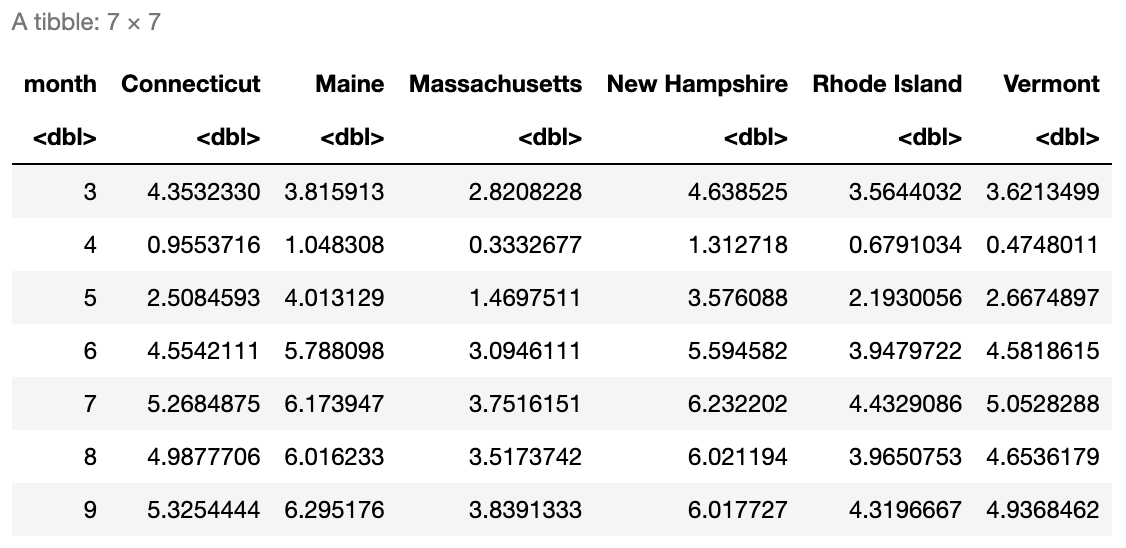
\includegraphics[width=1\textwidth,height=\textheight]{book/images/merging_data/mobility-pivot.png}

}

\caption{\label{fig-mobility-pivot}Pivoting Mobility Data.}

\end{figure}%

\begin{Shaded}
\begin{Highlighting}[]
\CommentTok{\# Insert your solution here:}
\end{Highlighting}
\end{Shaded}

The pivots seen so far were relatively simple in that there was only one
set of values we were pivoting on (e.g., the lockdown date, COVID-19
cases). The
\href{https://tidyr.tidyverse.org/articles/pivot.html}{\textbf{tidyr}
package} provides examples of more complex pivots that you might want to
apply to your data (Wickham, Vaughan, and Girlich
2023)\index{R packages!tidyr}.

\section{\texorpdfstring{Merging Data with Joins \index{data joins}
\index{merging data}}{Merging Data with Joins  }}\label{merging-data-with-joins}

In the last section, we saw how to manipulate our current data into new
formats. Now, we see how we can combine multiple data sources. Merging
two data frames is called \emph{joining}, and the functions we use to
perform this joining depends on how we want to match values between the
data frames. For example, we can join information about age and statin
use from \texttt{table1} and \texttt{table2} matching by name.

\begin{Shaded}
\begin{Highlighting}[]
\NormalTok{table1 }\OtherTok{\textless{}{-}} \FunctionTok{data.frame}\NormalTok{(}\AttributeTok{age =} \FunctionTok{c}\NormalTok{(}\DecValTok{14}\NormalTok{, }\DecValTok{26}\NormalTok{, }\DecValTok{32}\NormalTok{), }
                     \AttributeTok{name =} \FunctionTok{c}\NormalTok{(}\StringTok{"Alice"}\NormalTok{, }\StringTok{"Bob"}\NormalTok{, }\StringTok{"Alice"}\NormalTok{))}
\NormalTok{table2 }\OtherTok{\textless{}{-}} \FunctionTok{data.frame}\NormalTok{(}\AttributeTok{name =} \FunctionTok{c}\NormalTok{(}\StringTok{"Carol"}\NormalTok{, }\StringTok{"Bob"}\NormalTok{), }
                     \AttributeTok{statins =} \FunctionTok{c}\NormalTok{(}\ConstantTok{TRUE}\NormalTok{, }\ConstantTok{FALSE}\NormalTok{))}
\FunctionTok{full\_join}\NormalTok{(table1, table2, }\AttributeTok{by =} \StringTok{"name"}\NormalTok{)}
\CommentTok{\#\textgreater{}   age  name statins}
\CommentTok{\#\textgreater{} 1  14 Alice      NA}
\CommentTok{\#\textgreater{} 2  26   Bob   FALSE}
\CommentTok{\#\textgreater{} 3  32 Alice      NA}
\CommentTok{\#\textgreater{} 4  NA Carol    TRUE}
\end{Highlighting}
\end{Shaded}

The following list gives an overview of the different possible joins.
For each join type, we specify two tables, \texttt{table1} and
\texttt{table2}, and the \texttt{by} argument, which specifies the
columns used to match rows between tables.

\newpage

\textbf{Types of Joins}\index{data joins!types}:

\begin{itemize}
\tightlist
\item
  \texttt{left\_join(table1,\ table2,\ by)}: Joins each row of table1
  with all matches in table2.
  \index{R functions!left\textunderscore join()@\texttt{left\textunderscore join()}}\\
\item
  \texttt{right\_join(table1,\ table2,\ by)}: Joins each row of table2
  with all matches in table1 (the opposite of a left join)
  \index{R functions!right\textunderscore join()@\texttt{right\textunderscore join()}}\\
\item
  \texttt{inner\_join(table1,\ table2,\ by)}: Looks for all matches
  between rows in table1 and table2. Rows that do not find a match are
  dropped.
  \index{R functions!inner\textunderscore join()@\texttt{inner\textunderscore join()}}\\
\item
  \texttt{full\_join(table1,\ table2,\ by)}: Keeps all rows from both
  tables and joins those that match. Rows that do not find a match have
  NA values filled in.
  \index{R functions!full\textunderscore join()@\texttt{full\textunderscore join()}}\\
\item
  \texttt{semi\_join(table1,\ table2,\ by)}: Keeps all rows in table1
  that have a match in table2 but does not join to any information from
  table2.
  \index{R functions!semi\textunderscore join()@\texttt{semi\textunderscore join()}}\\
\item
  \texttt{anti\_join(table1,\ table2,\ by)}: Keeps all rows in table1
  that \emph{do not} have a match in table2 but does not join to any
  information from table2. The opposite of a semi-join.
  \index{R functions!anti\textunderscore join()@\texttt{anti\textunderscore join()}}
\end{itemize}

We first demonstrate a left-join using the
\texttt{left\_join()}\index{R functions!left\textunderscore join()@\texttt{left\textunderscore join()}}
function. This function takes in two data tables (table1 and table2) and
the columns to match rows by. In a left-join, for every row of table1,
we look for all matching rows in table2 and add any columns not used to
do the matching. Thus, every row in table1 corresponds to at least one
entry in the resulting table but possibly more if there are multiple
matches. In the subsequent code chunk, we use a left-join to add the
lockdown information to our \texttt{covidcases} data. In this case, the
first table is \texttt{covidcases} and we match by \texttt{state}. Since
the state column has a slightly different name in the two data frames
(``state'' in \texttt{covidcases} and ``State'' in
\texttt{lockdowndates}), we specify that \texttt{state} is equivalent to
\texttt{State} in the \texttt{by} argument.

\begin{Shaded}
\begin{Highlighting}[]
\NormalTok{covidcases\_full }\OtherTok{\textless{}{-}} \FunctionTok{left\_join}\NormalTok{(covidcases, lockdowndates, }
                             \AttributeTok{by =} \FunctionTok{c}\NormalTok{(}\StringTok{"state"} \OtherTok{=} \StringTok{"State"}\NormalTok{))}
\FunctionTok{head}\NormalTok{(covidcases\_full)}
\CommentTok{\#\textgreater{} \# A tibble: 6 x 8}
\CommentTok{\#\textgreater{}   state         county   week weekly\_cases weekly\_deaths date      }
\CommentTok{\#\textgreater{}   \textless{}chr\textgreater{}         \textless{}chr\textgreater{}   \textless{}dbl\textgreater{}        \textless{}int\textgreater{}         \textless{}int\textgreater{} \textless{}date\textgreater{}    }
\CommentTok{\#\textgreater{} 1 California    Marin       9            1             0 2020{-}02{-}23}
\CommentTok{\#\textgreater{} 2 California    Orange      9            3             0 2020{-}02{-}23}
\CommentTok{\#\textgreater{} 3 Florida       Manatee     9            1             0 2020{-}02{-}23}
\CommentTok{\#\textgreater{} 4 California    Napa        9            1             0 2020{-}02{-}23}
\CommentTok{\#\textgreater{} 5 New Hampshire Grafton     9            2             0 2020{-}02{-}23}
\CommentTok{\#\textgreater{} 6 Washington    Spokane     9            4             0 2020{-}02{-}23}
\CommentTok{\#\textgreater{} \# i 2 more variables: Lockdown\_Start \textless{}date\textgreater{}, Lockdown\_End \textless{}date\textgreater{}}
\end{Highlighting}
\end{Shaded}

These two new columns allow us to determine whether the start of each
recorded week was during a lockdown. We use the
\texttt{between()}\index{R functions!between()@\texttt{between()}}
function to create a new column \texttt{lockdown} before dropping the
two date columns. We can check that this column worked as expected by
choosing a single county to look at.

\begin{Shaded}
\begin{Highlighting}[]
\NormalTok{covidcases\_full }\OtherTok{\textless{}{-}}\NormalTok{ covidcases\_full }\SpecialCharTok{\%\textgreater{}\%}
  \FunctionTok{mutate}\NormalTok{(}\AttributeTok{lockdown =} \FunctionTok{between}\NormalTok{(date, Lockdown\_Start, Lockdown\_End)) }\SpecialCharTok{\%\textgreater{}\%}
  \FunctionTok{select}\NormalTok{(}\SpecialCharTok{{-}}\FunctionTok{c}\NormalTok{(Lockdown\_Start, Lockdown\_End)) }
\NormalTok{covidcases\_full }\SpecialCharTok{\%\textgreater{}\%}
  \FunctionTok{filter}\NormalTok{(state }\SpecialCharTok{==} \StringTok{"Alabama"}\NormalTok{, county }\SpecialCharTok{==} \StringTok{"Jefferson"}\NormalTok{, }
\NormalTok{         date }\SpecialCharTok{\textless{}=} \FunctionTok{as.Date}\NormalTok{(}\StringTok{"2020{-}05{-}10"}\NormalTok{))}
\CommentTok{\#\textgreater{} \# A tibble: 10 x 7}
\CommentTok{\#\textgreater{}   state   county     week weekly\_cases weekly\_deaths date       lockdown}
\CommentTok{\#\textgreater{}   \textless{}chr\textgreater{}   \textless{}chr\textgreater{}     \textless{}dbl\textgreater{}        \textless{}int\textgreater{}         \textless{}int\textgreater{} \textless{}date\textgreater{}     \textless{}lgl\textgreater{}   }
\CommentTok{\#\textgreater{} 1 Alabama Jefferson    11           21             0 2020{-}03{-}08 FALSE   }
\CommentTok{\#\textgreater{} 2 Alabama Jefferson    12           70             0 2020{-}03{-}15 FALSE   }
\CommentTok{\#\textgreater{} 3 Alabama Jefferson    13          191             0 2020{-}03{-}22 FALSE   }
\CommentTok{\#\textgreater{} 4 Alabama Jefferson    14          179            12 2020{-}03{-}29 FALSE   }
\CommentTok{\#\textgreater{} 5 Alabama Jefferson    15          159             4 2020{-}04{-}05 TRUE    }
\CommentTok{\#\textgreater{} \# i 5 more rows}
\end{Highlighting}
\end{Shaded}

We now want to add in the mobility data. In the previous join, we wanted
to keep any observation in \texttt{covidcases} regardless if it was in
the \texttt{lockdowndates} data frame. Therefore, we used a left-join.
In this case, we only want to keep observations that have mobility data
for that state on each date. This indicates that we want to use an
\emph{inner-join}. The function
\texttt{inner\_join()}\index{R functions!inner\textunderscore join()@\texttt{inner\textunderscore join()}}
takes in two data tables (table1 and table2) and the columns to match
rows by. The function only keeps rows in table1 that match to a row in
table2. Again, those columns in table2 not used to match with table1 are
added to the resulting outcome. In this case, we match by both state and
date.

\begin{Shaded}
\begin{Highlighting}[]
\NormalTok{covidcases\_full }\OtherTok{\textless{}{-}} \FunctionTok{inner\_join}\NormalTok{(covidcases\_full, mobility, }
                              \AttributeTok{by =} \FunctionTok{c}\NormalTok{(}\StringTok{"state"}\NormalTok{, }\StringTok{"date"}\NormalTok{)) }\SpecialCharTok{\%\textgreater{}\%}
  \FunctionTok{select}\NormalTok{(}\SpecialCharTok{{-}}\FunctionTok{c}\NormalTok{(samples, m50\_index))}
\FunctionTok{head}\NormalTok{(covidcases\_full)}
\CommentTok{\#\textgreater{} \# A tibble: 6 x 8}
\CommentTok{\#\textgreater{}   state      county  week weekly\_cases weekly\_deaths date       lockdown}
\CommentTok{\#\textgreater{}   \textless{}chr\textgreater{}      \textless{}chr\textgreater{}  \textless{}dbl\textgreater{}        \textless{}int\textgreater{}         \textless{}int\textgreater{} \textless{}date\textgreater{}     \textless{}lgl\textgreater{}   }
\CommentTok{\#\textgreater{} 1 Florida    Okalo\textasciitilde{}    10            1             0 2020{-}03{-}01 FALSE   }
\CommentTok{\#\textgreater{} 2 Georgia    Charl\textasciitilde{}    10            1             0 2020{-}03{-}01 FALSE   }
\CommentTok{\#\textgreater{} 3 Massachus\textasciitilde{} Essex     10            1             0 2020{-}03{-}01 FALSE   }
\CommentTok{\#\textgreater{} 4 New York   Rockl\textasciitilde{}    10            6             0 2020{-}03{-}01 FALSE   }
\CommentTok{\#\textgreater{} 5 Indiana    Hendr\textasciitilde{}    10            2             0 2020{-}03{-}01 FALSE   }
\CommentTok{\#\textgreater{} 6 California Marin     10            1             0 2020{-}03{-}01 FALSE   }
\CommentTok{\#\textgreater{} \# i 1 more variable: m50 \textless{}dbl\textgreater{}}
\end{Highlighting}
\end{Shaded}

\subsection{Practice Question}\label{practice-question-12}

Look at the two data frames, \texttt{df\_A} and \texttt{df\_B}, defined
in the following code. What kind of join would produce the data frame in
Figure~\ref{fig-joining-data}? Perform this join yourself.

\begin{figure}

\centering{

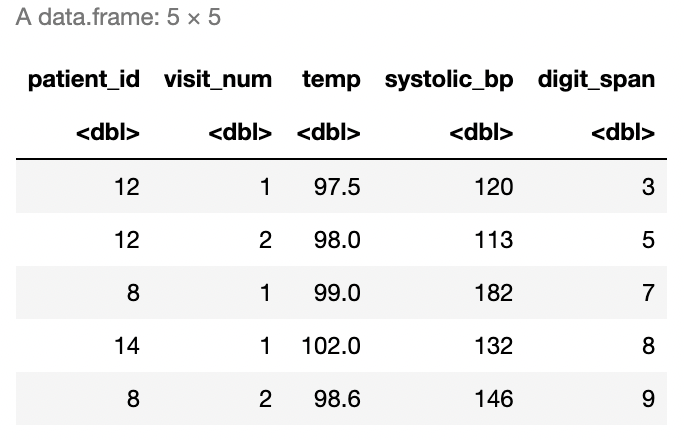
\includegraphics[width=0.8\textwidth,height=\textheight]{book/images/merging_data/joining-data.png}

}

\caption{\label{fig-joining-data}Joining Data.}

\end{figure}%

\begin{Shaded}
\begin{Highlighting}[]
\NormalTok{df\_A }\OtherTok{\textless{}{-}} \FunctionTok{data.frame}\NormalTok{(}\AttributeTok{patient\_id =} \FunctionTok{c}\NormalTok{(}\DecValTok{12}\NormalTok{, }\DecValTok{9}\NormalTok{, }\DecValTok{12}\NormalTok{, }\DecValTok{8}\NormalTok{, }\DecValTok{14}\NormalTok{, }\DecValTok{8}\NormalTok{), }
                  \AttributeTok{visit\_num =} \FunctionTok{c}\NormalTok{(}\DecValTok{1}\NormalTok{, }\DecValTok{1}\NormalTok{, }\DecValTok{2}\NormalTok{, }\DecValTok{1}\NormalTok{, }\DecValTok{1}\NormalTok{, }\DecValTok{2}\NormalTok{), }
                  \AttributeTok{temp =} \FunctionTok{c}\NormalTok{(}\FloatTok{97.5}\NormalTok{, }\DecValTok{96}\NormalTok{, }\DecValTok{98}\NormalTok{, }\DecValTok{99}\NormalTok{, }\DecValTok{102}\NormalTok{, }\FloatTok{98.6}\NormalTok{), }
                  \AttributeTok{systolic\_bp =} \FunctionTok{c}\NormalTok{(}\DecValTok{120}\NormalTok{, }\DecValTok{138}\NormalTok{, }\DecValTok{113}\NormalTok{, }\DecValTok{182}\NormalTok{, }\DecValTok{132}\NormalTok{, }\DecValTok{146}\NormalTok{))}
\NormalTok{df\_A}
\CommentTok{\#\textgreater{}   patient\_id visit\_num  temp systolic\_bp}
\CommentTok{\#\textgreater{} 1         12         1  97.5         120}
\CommentTok{\#\textgreater{} 2          9         1  96.0         138}
\CommentTok{\#\textgreater{} 3         12         2  98.0         113}
\CommentTok{\#\textgreater{} 4          8         1  99.0         182}
\CommentTok{\#\textgreater{} 5         14         1 102.0         132}
\CommentTok{\#\textgreater{} 6          8         2  98.6         146}
\NormalTok{df\_B }\OtherTok{\textless{}{-}} \FunctionTok{data.frame}\NormalTok{(}\AttributeTok{patient\_id =} \FunctionTok{c}\NormalTok{(}\DecValTok{12}\NormalTok{, }\DecValTok{12}\NormalTok{, }\DecValTok{12}\NormalTok{, }\DecValTok{8}\NormalTok{, }\DecValTok{8}\NormalTok{, }\DecValTok{8}\NormalTok{, }\DecValTok{14}\NormalTok{, }\DecValTok{14}\NormalTok{), }
                   \AttributeTok{visit\_num =} \FunctionTok{c}\NormalTok{(}\DecValTok{1}\NormalTok{, }\DecValTok{2}\NormalTok{, }\DecValTok{3}\NormalTok{, }\DecValTok{1}\NormalTok{, }\DecValTok{2}\NormalTok{, }\DecValTok{3}\NormalTok{, }\DecValTok{1}\NormalTok{, }\DecValTok{2}\NormalTok{),}
                   \AttributeTok{digit\_span =} \FunctionTok{c}\NormalTok{(}\DecValTok{3}\NormalTok{, }\DecValTok{5}\NormalTok{, }\DecValTok{7}\NormalTok{, }\DecValTok{7}\NormalTok{, }\DecValTok{9}\NormalTok{, }\DecValTok{5}\NormalTok{, }\DecValTok{8}\NormalTok{, }\DecValTok{7}\NormalTok{))}
\NormalTok{df\_B}
\CommentTok{\#\textgreater{}   patient\_id visit\_num digit\_span}
\CommentTok{\#\textgreater{} 1         12         1          3}
\CommentTok{\#\textgreater{} 2         12         2          5}
\CommentTok{\#\textgreater{} 3         12         3          7}
\CommentTok{\#\textgreater{} 4          8         1          7}
\CommentTok{\#\textgreater{} 5          8         2          9}
\CommentTok{\#\textgreater{} 6          8         3          5}
\CommentTok{\#\textgreater{} 7         14         1          8}
\CommentTok{\#\textgreater{} 8         14         2          7}
\end{Highlighting}
\end{Shaded}

\begin{Shaded}
\begin{Highlighting}[]
\CommentTok{\# Insert your solution here:}
\end{Highlighting}
\end{Shaded}

\section{Exercises}\label{exercises-4}

\begin{enumerate}
\def\labelenumi{\arabic{enumi}.}
\item
  Take a look at the provided code. What is wrong with it? Hint: think
  about what causes the warning message.

\begin{Shaded}
\begin{Highlighting}[]
\NormalTok{visit\_info }\OtherTok{\textless{}{-}} \FunctionTok{data.frame}\NormalTok{(}
  \AttributeTok{name.f =} \FunctionTok{c}\NormalTok{(}\StringTok{"Phillip"}\NormalTok{, }\StringTok{"Phillip"}\NormalTok{, }\StringTok{"Phillip"}\NormalTok{, }\StringTok{"Jessica"}\NormalTok{, }
             \StringTok{"Jessica"}\NormalTok{),}
  \AttributeTok{name.l =} \FunctionTok{c}\NormalTok{(}\StringTok{"Johnson"}\NormalTok{, }\StringTok{"Johnson"}\NormalTok{, }\StringTok{"Richards"}\NormalTok{, }\StringTok{"Smith"}\NormalTok{, }
             \StringTok{"Abrams"}\NormalTok{),}
  \AttributeTok{measure =} \FunctionTok{c}\NormalTok{(}\StringTok{"height"}\NormalTok{, }\StringTok{"age"}\NormalTok{, }\StringTok{"age"}\NormalTok{, }\StringTok{"age"}\NormalTok{, }\StringTok{"height"}\NormalTok{),}
  \AttributeTok{measurement =} \FunctionTok{c}\NormalTok{(}\DecValTok{45}\NormalTok{, }\DecValTok{186}\NormalTok{, }\DecValTok{50}\NormalTok{, }\DecValTok{37}\NormalTok{, }\DecValTok{156}\NormalTok{)}
\NormalTok{)}

\NormalTok{contact\_info }\OtherTok{\textless{}{-}} \FunctionTok{data.frame}\NormalTok{(}
\AttributeTok{first\_name =} \FunctionTok{c}\NormalTok{(}\StringTok{"Phillip"}\NormalTok{, }\StringTok{"Phillip"}\NormalTok{, }\StringTok{"Jessica"}\NormalTok{, }\StringTok{"Margaret"}\NormalTok{),}
\AttributeTok{last\_name =} \FunctionTok{c}\NormalTok{(}\StringTok{"Richards"}\NormalTok{, }\StringTok{"Johnson"}\NormalTok{, }\StringTok{"Smith"}\NormalTok{, }\StringTok{"Reynolds"}\NormalTok{),}
\AttributeTok{email =} \FunctionTok{c}\NormalTok{(}\StringTok{"pr@aol.com"}\NormalTok{, }\StringTok{"phillipj@gmail.com"}\NormalTok{, }
          \StringTok{"jesssmith@brown.edu"}\NormalTok{, }\StringTok{"marg@hotmail.com"}\NormalTok{)}
\NormalTok{)}

\FunctionTok{left\_join}\NormalTok{(visit\_info, contact\_info, }
          \AttributeTok{by =} \FunctionTok{c}\NormalTok{(}\StringTok{"name.f"} \OtherTok{=} \StringTok{"first\_name"}\NormalTok{))}
\CommentTok{\#\textgreater{} Warning in left\_join(visit\_info, contact\_info, by = c(name.f = "first\_name")): Detected an unexpected many{-}to{-}many relationship between \textasciigrave{}x\textasciigrave{} and \textasciigrave{}y\textasciigrave{}.}
\CommentTok{\#\textgreater{} i Row 1 of \textasciigrave{}x\textasciigrave{} matches multiple rows in \textasciigrave{}y\textasciigrave{}.}
\CommentTok{\#\textgreater{} i Row 1 of \textasciigrave{}y\textasciigrave{} matches multiple rows in \textasciigrave{}x\textasciigrave{}.}
\CommentTok{\#\textgreater{} i If a many{-}to{-}many relationship is expected, set \textasciigrave{}relationship =}
\CommentTok{\#\textgreater{}   "many{-}to{-}many"\textasciigrave{} to silence this warning.}
\CommentTok{\#\textgreater{}    name.f   name.l measure measurement last\_name               email}
\CommentTok{\#\textgreater{} 1 Phillip  Johnson  height          45  Richards          pr@aol.com}
\CommentTok{\#\textgreater{} 2 Phillip  Johnson  height          45   Johnson  phillipj@gmail.com}
\CommentTok{\#\textgreater{} 3 Phillip  Johnson     age         186  Richards          pr@aol.com}
\CommentTok{\#\textgreater{} 4 Phillip  Johnson     age         186   Johnson  phillipj@gmail.com}
\CommentTok{\#\textgreater{} 5 Phillip Richards     age          50  Richards          pr@aol.com}
\CommentTok{\#\textgreater{} 6 Phillip Richards     age          50   Johnson  phillipj@gmail.com}
\CommentTok{\#\textgreater{} 7 Jessica    Smith     age          37     Smith jesssmith@brown.edu}
\CommentTok{\#\textgreater{} 8 Jessica   Abrams  height         156     Smith jesssmith@brown.edu}
\end{Highlighting}
\end{Shaded}
\item
  First, use the \texttt{covidcases} data to create a new data frame
  called \texttt{sub\_cases} containing the total number of cases by
  month for the states of California, Michigan, Connecticut, Rhode
  Island, Ohio, New York, and Massachusetts. Then, manipulate the
  \texttt{mobility} data to calculate the average \texttt{m50} mobility
  measure for each month. Finally, merge these two datasets using an
  appropriate joining function.
\item
  Convert the \texttt{sub\_cases} data frame from the previous exercise
  to wide format so that each row displays the cases in each state for a
  single month. Then, add on the average m50 overall for each month as
  an additional column using a join function.
\end{enumerate}

\chapter{Visualization with ggplot2}\label{sec-ggplot2}

The package \textbf{ggplot2} (Wickham 2016) \index{R packages!ggplot2}
is another useful package in the
\textbf{tidyverse}\index{R packages!tidyverse} that allows statisticians
to use visualizations to communicate key findings and results in a
compelling format. In this chapter, we learn about the three main
components in a ggplot object and then expand on that format by learning
more about the different layers we can use to create various plots. As
with the \textbf{dplyr} functions, there are many functions to cover,
and they build upon one another.

The three packages we use in this chapter are \textbf{tidyverse},
\textbf{HDSinRdata}\index{R packages!HDSinRdata}, and
\textbf{patchwork}\index{R packages!patchwork} (Pedersen 2022), the last
of which is a nice package for combining multiple plots together into a
single figure. We use the data from the Pittsburgh pain clinic (Alter et
al. 2021) \index{Datasets!pain@\texttt{pain}} introduced in
Chapter~\ref{sec-data-files} to create our visuals. You can refresh your
memory about this data by reading the data documentation. For the
purposes of this chapter, we take a sample of 5,000 patients that are
complete cases at baseline to reduce the computation time to display
each plot. You can ignore how the code used to find this sample works.

\begin{Shaded}
\begin{Highlighting}[]
\FunctionTok{library}\NormalTok{(tidyverse)}
\FunctionTok{library}\NormalTok{(HDSinRdata)}
\FunctionTok{library}\NormalTok{(patchwork)}
\FunctionTok{data}\NormalTok{(pain)}

\CommentTok{\# sampling data}
\FunctionTok{set.seed}\NormalTok{(}\DecValTok{5}\NormalTok{)}
\NormalTok{pain\_df\_sub }\OtherTok{\textless{}{-}} \FunctionTok{subset}\NormalTok{(pain, }
                      \AttributeTok{select =} \SpecialCharTok{{-}}\FunctionTok{c}\NormalTok{(PAIN\_INTENSITY\_AVERAGE.FOLLOW\_UP))}
\NormalTok{pain\_df }\OtherTok{\textless{}{-}}\NormalTok{ pain[}\FunctionTok{complete.cases}\NormalTok{(pain\_df\_sub), ]}
\NormalTok{pain\_df }\OtherTok{\textless{}{-}}\NormalTok{ pain\_df[}\FunctionTok{sample}\NormalTok{(}\DecValTok{1}\SpecialCharTok{:}\FunctionTok{nrow}\NormalTok{(pain\_df), }\DecValTok{5000}\NormalTok{, }\AttributeTok{replace =} \ConstantTok{FALSE}\NormalTok{),] }
\end{Highlighting}
\end{Shaded}

\section{Intro to ggplot}\label{intro-to-ggplot}

We'll begin by demonstrating how to create a scatter plot
\index{plots!scatter plot} in \textbf{ggplot2} to introduce the three
key elements of a \texttt{ggplot2}
object\index{ggplot2!ggplot2 objects}. Specifically, we create a scatter
plot of a patient's depression vs.~anxiety score. To start a graph, we
can use the
\texttt{ggplot()}\index{R functions!ggplot()@\texttt{ggplot()}} function
to create a \texttt{ggplot} object as shown in the following code. Note
that this brings up a gray box; this is the base that we build up from.

\begin{Shaded}
\begin{Highlighting}[]
\FunctionTok{ggplot}\NormalTok{()}
\end{Highlighting}
\end{Shaded}

\begin{center}

\includegraphics[width=1\textwidth,height=\textheight]{book/visualization_ggplot_files/figure-pdf/unnamed-chunk-2-1.pdf}
\end{center}

Next, we can begin adding layers to our \texttt{ggplot} object. One type
of layer is a \textbf{geom}\index{ggplot2!geoms}, which creates a
geometric object. In the next code chunk, we use the
\texttt{geom\_point()}\index{R functions!geom\textunderscore point()@\texttt{geom\textunderscore point()}}
function to add a scatter plot layer. For this function, we first need
to specify which data we want to use, and then we need to tell R how to
use that data to create the scatter plot using the \texttt{aes()}
function, which creates an \textbf{aesthetic}\index{ggplot2!aesthetic}.
For a scatter plot, we need to at least specify the x-axis and y-axis in
the aesthetic. Both the data and the aesthetic can either be specified
in our initial \texttt{ggplot()} function, which passes this information
to all future layers, or in the \texttt{geom\_point()} function itself.
In the following code, we specify the aesthetic in the geom function but
also include two alternative ways to code the same image in the
subsequent code chunk. The resulting plot shows a fairly linear
relationship between anxiety and depression.

\begin{Shaded}
\begin{Highlighting}[]
\FunctionTok{ggplot}\NormalTok{(pain\_df) }\SpecialCharTok{+} \FunctionTok{geom\_point}\NormalTok{(}\FunctionTok{aes}\NormalTok{(}\AttributeTok{x=}\NormalTok{PROMIS\_ANXIETY, }
                                 \AttributeTok{y =}\NormalTok{ PROMIS\_DEPRESSION))}
\end{Highlighting}
\end{Shaded}

\begin{center}
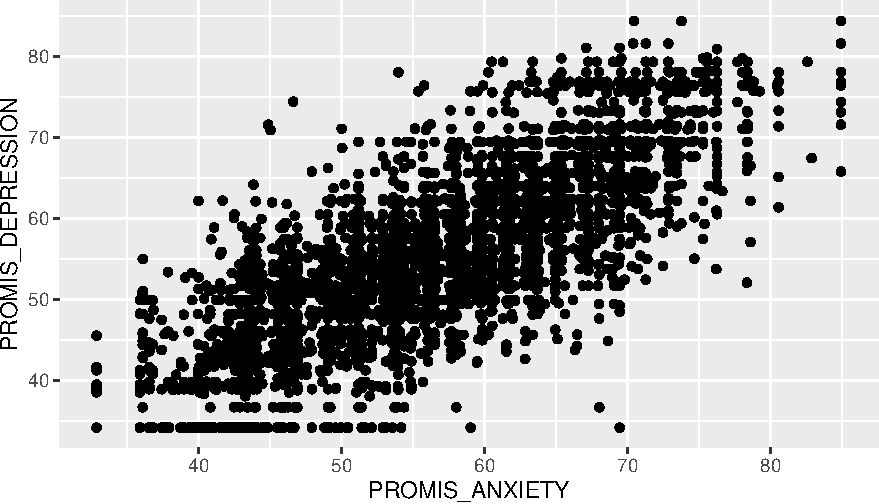
\includegraphics[width=1\textwidth,height=\textheight]{book/visualization_ggplot_files/figure-pdf/unnamed-chunk-3-1.pdf}
\end{center}

\begin{Shaded}
\begin{Highlighting}[]
\CommentTok{\# Alternative 1:}
\FunctionTok{ggplot}\NormalTok{(pain\_df, }\FunctionTok{aes}\NormalTok{(}\AttributeTok{x =}\NormalTok{ PROMIS\_ANXIETY, }\AttributeTok{y =}\NormalTok{ PROMIS\_DEPRESSION)) }\SpecialCharTok{+} 
  \FunctionTok{geom\_point}\NormalTok{()}
\CommentTok{\# Alternative 2:}
\FunctionTok{ggplot}\NormalTok{() }\SpecialCharTok{+} 
  \FunctionTok{geom\_point}\NormalTok{(}\AttributeTok{data =}\NormalTok{ pain\_df, }\FunctionTok{aes}\NormalTok{(}\AttributeTok{x =}\NormalTok{ PROMIS\_ANXIETY, }
                                 \AttributeTok{y =}\NormalTok{ PROMIS\_DEPRESSION))}
\end{Highlighting}
\end{Shaded}

If we want to improve our plot, we may want to add different labels
\index{ggplot2!labels} and a title. To do so, we use the
\texttt{labs()}\index{R functions!labs()@\texttt{labs()}} function to
add a layer in which we can specify all labels. Additionally, I have
passed more information to the geometry layer by changing the color,
size, and shape of the points. These things are specified outside of the
\texttt{aes()}\index{R functions!aes()@\texttt{aes()}} function since
they do not come from the data; every point has the same color, size,
and shape in this example.

\begin{Shaded}
\begin{Highlighting}[]
\FunctionTok{ggplot}\NormalTok{(pain\_df)}\SpecialCharTok{+}
  \FunctionTok{geom\_point}\NormalTok{(}\FunctionTok{aes}\NormalTok{(}\AttributeTok{x =}\NormalTok{ PROMIS\_ANXIETY, }\AttributeTok{y =}\NormalTok{ PROMIS\_DEPRESSION), }
             \AttributeTok{color =} \StringTok{"blue"}\NormalTok{, }\AttributeTok{size =} \DecValTok{2}\NormalTok{, }\AttributeTok{shape =} \DecValTok{5}\NormalTok{) }\SpecialCharTok{+} 
  \FunctionTok{labs}\NormalTok{(}\AttributeTok{x =} \StringTok{"PROMIS Anxiety Score"}\NormalTok{, }\AttributeTok{y =} \StringTok{"PROMIS Depression Score"}\NormalTok{, }
       \AttributeTok{title =} \StringTok{"Depression vs Anxiety Scores"}\NormalTok{)}
\end{Highlighting}
\end{Shaded}

\begin{center}
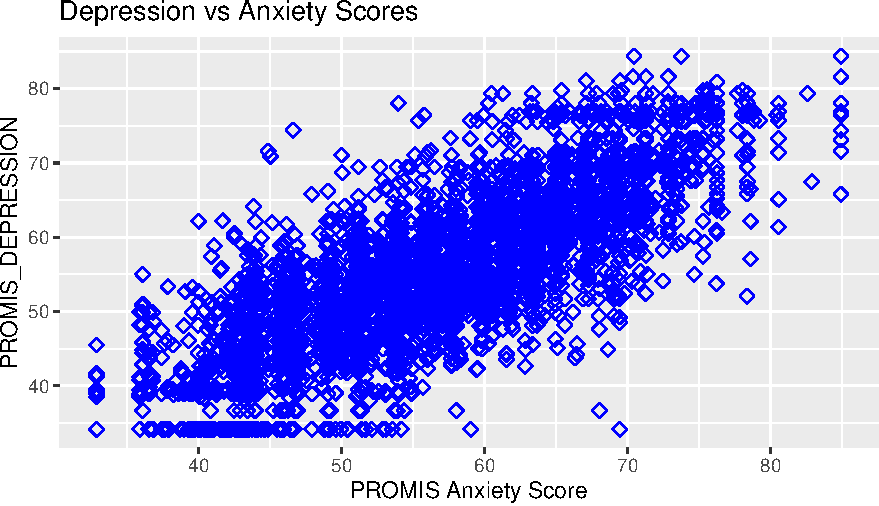
\includegraphics[width=1\textwidth,height=\textheight]{book/visualization_ggplot_files/figure-pdf/unnamed-chunk-5-1.pdf}
\end{center}

Let's create another example. This time, I create a histogram for
initial recorded pain level. To find the corresponding geom for the type
of plot we'd like to make, we can use the
\href{https://posit.co/wp-content/uploads/2022/10/data-visualization-1.pdf}{data
visualization cheat sheet from Posit}. The first page lists all the geom
options available along with what aesthetics we can set for each option.
For example, here we are interested in plotting the distribution of one
continuous variable, and under the
\texttt{geom\_histogram()}\index{R functions!geom\textunderscore histogram()@\texttt{geom\textunderscore histogram()}}
function we can see that we can specify \texttt{x} (the variable whose
distribution we want to plot) as well as \texttt{binwidth}, \texttt{y},
\texttt{alpha}, \texttt{color}, \texttt{fill}, \texttt{linetype},
\texttt{size}, and \texttt{weight}. By default, the \texttt{y} value in
a histogram is the count for each bin.

In the following code, you can see that we updated the color
(\texttt{color}), fill (\texttt{fill}), and opacity (\texttt{alpha}) of
our histogram bars and updated the number of bins to be 11 (to account
for the possible values 0-10). Additionally, we used the
\texttt{theme\_minimal()}\index{R functions!theme\textunderscore minimal()@\texttt{theme\textunderscore minimal()}}
function to change the background colors used. You can find the
available themes \index{ggplot2!themes} on the second page of the cheat
sheet. Try changing the theme of the following plot to
\texttt{theme\_bw()}.

\begin{Shaded}
\begin{Highlighting}[]
\FunctionTok{ggplot}\NormalTok{(pain\_df)}\SpecialCharTok{+}
  \FunctionTok{geom\_histogram}\NormalTok{(}\FunctionTok{aes}\NormalTok{(}\AttributeTok{x =}\NormalTok{ PAIN\_INTENSITY\_AVERAGE), }\AttributeTok{color =} \StringTok{"violetred"}\NormalTok{, }
                 \AttributeTok{fill =} \StringTok{"lightblue"}\NormalTok{, }\AttributeTok{alpha =} \FloatTok{0.5}\NormalTok{, }\AttributeTok{bins =} \DecValTok{11}\NormalTok{) }\SpecialCharTok{+}
  \FunctionTok{labs}\NormalTok{(}\AttributeTok{x =} \StringTok{"Patient Reported Pain Intensity"}\NormalTok{, }\AttributeTok{y =} \StringTok{"Count"}\NormalTok{)}\SpecialCharTok{+}
  \FunctionTok{theme\_minimal}\NormalTok{()}
\end{Highlighting}
\end{Shaded}

\begin{center}
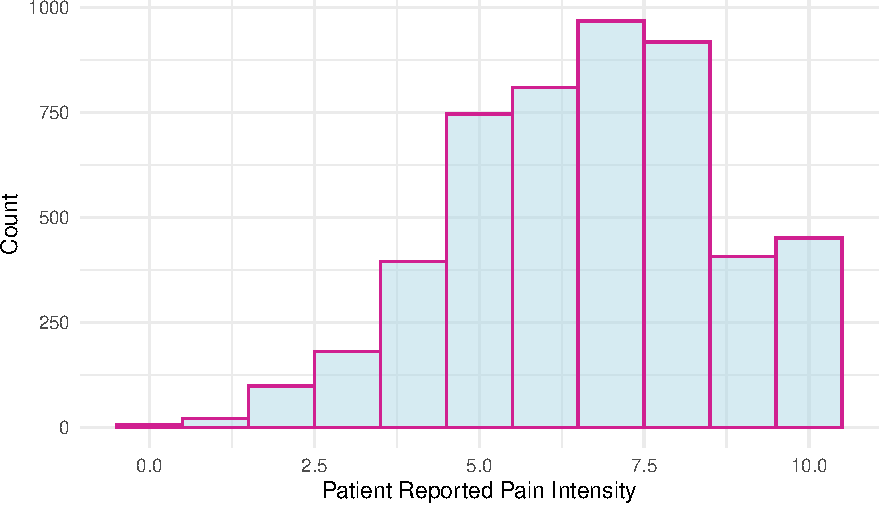
\includegraphics[width=1\textwidth,height=\textheight]{book/visualization_ggplot_files/figure-pdf/unnamed-chunk-6-1.pdf}
\end{center}

\subsection{Practice Question}\label{practice-question-13}

Recreate Figure~\ref{fig-line-plot}.

\begin{figure}

\centering{

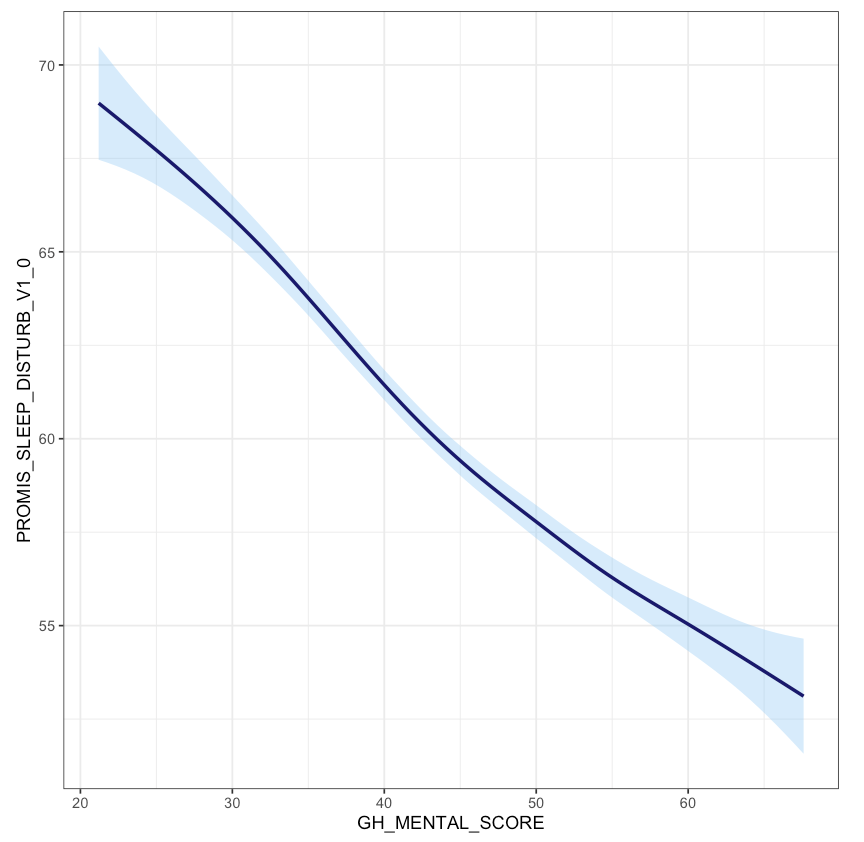
\includegraphics[width=0.8\textwidth,height=\textheight]{book/images/visualization_ggplot/line-plot.png}

}

\caption{\label{fig-line-plot}Line Plot.}

\end{figure}%

\begin{Shaded}
\begin{Highlighting}[]
\CommentTok{\# Insert your solution here: }
\end{Highlighting}
\end{Shaded}

\section{Adjusting the Axes and
Aesthetics}\label{adjusting-the-axes-and-aesthetics}

We can further control how each aesthetic element is displayed using
\emph{scale}
functions\index{ggplot2!scale functions}\index{ggplot2!aesthetics}. For
example, suppose that I want to update the previous plot. In particular,
I first want to update the x-axis to display all of the values 0 to 10
instead of 0, 2.5, 5, etc.. To update the x-axis, I need to find the
corresponding scale function for x with continuous values. This function
is
\texttt{scale\_x\_continuous()}\index{R functions!scale\textunderscore x\textunderscore continuous()@\texttt{scale\textunderscore x\textunderscore continuous()}},
which allows me to specify limits (\texttt{limits}), breaks
(\texttt{breaks}), and labels (\texttt{labels}). The scale functions can
be found on the second sheet of the cheat sheet. In this case, I just
want to update the breaks to be all integer values from 0 to 10.

\begin{Shaded}
\begin{Highlighting}[]
\FunctionTok{ggplot}\NormalTok{(pain\_df)}\SpecialCharTok{+}
  \FunctionTok{geom\_histogram}\NormalTok{(}\FunctionTok{aes}\NormalTok{(}\AttributeTok{x =}\NormalTok{ PAIN\_INTENSITY\_AVERAGE), }\AttributeTok{color =} \StringTok{"violetred"}\NormalTok{, }
                 \AttributeTok{fill =} \StringTok{"lightblue"}\NormalTok{, }\AttributeTok{alpha =} \FloatTok{0.5}\NormalTok{, }\AttributeTok{bins =} \DecValTok{11}\NormalTok{) }\SpecialCharTok{+}
  \FunctionTok{labs}\NormalTok{(}\AttributeTok{x =} \StringTok{"Patient Reported Pain Intensity"}\NormalTok{, }\AttributeTok{y =} \StringTok{"Count"}\NormalTok{)}\SpecialCharTok{+}
  \FunctionTok{scale\_x\_continuous}\NormalTok{(}\AttributeTok{breaks =} \DecValTok{0}\SpecialCharTok{:}\DecValTok{10}\NormalTok{)}\SpecialCharTok{+}
  \FunctionTok{theme\_minimal}\NormalTok{()}
\end{Highlighting}
\end{Shaded}

\begin{center}
\includegraphics[width=1\textwidth,height=\textheight]{book/visualization_ggplot_files/figure-pdf/unnamed-chunk-8-1.pdf}
\end{center}

Now, let's take a more complex example. The following plot shows each
patient's reported sleep disturbance vs.~physical function and colors
each point by their reported pain intensity. Since some points might
overlap in values, we added \texttt{position="jitter"} to the
\texttt{geom\_point()} function to jitter the points, which corresponds
to adding some random noise to each point's position. As presented, this
plot is difficult to interpret. For example, the color of pain intensity
makes it hard to see how pain changes, and the legend title needs to be
simpler.

\begin{Shaded}
\begin{Highlighting}[]
\FunctionTok{ggplot}\NormalTok{(pain\_df)}\SpecialCharTok{+}
  \FunctionTok{geom\_point}\NormalTok{(}\FunctionTok{aes}\NormalTok{(}\AttributeTok{x =}\NormalTok{ PROMIS\_PHYSICAL\_FUNCTION, }
                 \AttributeTok{y =}\NormalTok{ PROMIS\_SLEEP\_DISTURB\_V1\_0, }
                 \AttributeTok{color =}\NormalTok{ PAIN\_INTENSITY\_AVERAGE), }\AttributeTok{position=}\StringTok{"jitter"}\NormalTok{)}
\end{Highlighting}
\end{Shaded}

\begin{center}
\includegraphics[width=1\textwidth,height=\textheight]{book/visualization_ggplot_files/figure-pdf/unnamed-chunk-9-1.pdf}
\end{center}

Suppose that we wanted to visualize the pain intensity and sleep
disturbance for patients with below-average physical function. Note that
both sleep disturbance and physical function are reported as T-Scores,
meaning that the raw scores have been converted to a standardized score
with mean 50 and standard deviation 10 within the population. We can use
the scale functions to update our axes and labels to reflect this
information. As before, we need to use the
\texttt{scale\_x\_continuous()} function to update the x-axis for a
continuous variable. In this case, we update the limits (to restrict to
below-average physical function), breaks, and labels. We similarly
update the y-axis.

Lastly, suppose we want to update the color aesthetic. As before, this
aesthetic corresponds to a continuous variable. The cheat sheet provides
several possible scale functions depending on how we want to specify the
color gradient. We choose the
\texttt{scale\_color\_gradient()}\index{R functions!scale\textunderscore color\textunderscore gradient()@\texttt{scale\textunderscore color\textunderscore gradient()}}
function, since this allows us to specify the low and high end colors.
We can also specify the breaks for the legend values similar to how we
specified the breaks for the x- and y-axes. The argument \texttt{name}
also allows us to rename this legend. The palette then converts this to
a continuous color gradient. Note that in contrast to the
\texttt{scale\_color\_gradient()} function that we chose to use for this
example, the functions
\texttt{scale\_color\_gradient2()}\index{R functions!scale\textunderscore color\textunderscore gradient2()@\texttt{scale\textunderscore color\textunderscore gradient2()}}
and
\texttt{scale\_color\_gradientn()}\index{R functions!scale\textunderscore color\textunderscore gradientn()@\texttt{scale\textunderscore color\textunderscore gradientn()}}
allow you to specify more color points in the gradient rather than just
the two extreme colors.

We can observe that decreased physical function is associated with
higher sleep disturbance, and that those with worse physical function
and worse sleep disturbance tend to have higher reported pain. Note that
this time we receive a warning message, which is because our axis limits
have cut off some points. To avoid this message, we could use the
function
\texttt{coord\_cartesian()}\index{R functions!coord\textunderscore cartesian()@\texttt{coord\textunderscore cartesian()}}
to specify our limits which clips the values rather than removing points
outside the limits.

\begin{Shaded}
\begin{Highlighting}[]
\FunctionTok{ggplot}\NormalTok{(pain\_df)}\SpecialCharTok{+}
  \FunctionTok{geom\_point}\NormalTok{(}\FunctionTok{aes}\NormalTok{(}\AttributeTok{x =}\NormalTok{ PROMIS\_PHYSICAL\_FUNCTION, }
                 \AttributeTok{y =}\NormalTok{ PROMIS\_SLEEP\_DISTURB\_V1\_0, }
                 \AttributeTok{color =}\NormalTok{ PAIN\_INTENSITY\_AVERAGE), }
             \AttributeTok{position =} \StringTok{"jitter"}\NormalTok{, }\AttributeTok{alpha =} \FloatTok{0.5}\NormalTok{) }\SpecialCharTok{+}
  \FunctionTok{scale\_x\_continuous}\NormalTok{(}\AttributeTok{limits =} \FunctionTok{c}\NormalTok{(}\DecValTok{15}\NormalTok{,}\DecValTok{50}\NormalTok{), }\AttributeTok{breaks =} \FunctionTok{c}\NormalTok{(}\DecValTok{20}\NormalTok{, }\DecValTok{30}\NormalTok{, }\DecValTok{40}\NormalTok{, }\DecValTok{50}\NormalTok{), }
                     \AttributeTok{labels =} \FunctionTok{c}\NormalTok{(}\StringTok{"{-}3 SD"}\NormalTok{, }\StringTok{"{-}2 SD"}\NormalTok{, }\StringTok{"{-}1 SD"}\NormalTok{, }
                                \StringTok{"Pop Mean"}\NormalTok{)) }\SpecialCharTok{+} 
  \FunctionTok{scale\_y\_continuous}\NormalTok{(}\AttributeTok{breaks =} \FunctionTok{c}\NormalTok{(}\DecValTok{40}\NormalTok{, }\DecValTok{50}\NormalTok{, }\DecValTok{60}\NormalTok{, }\DecValTok{70}\NormalTok{, }\DecValTok{80}\NormalTok{), }
                     \AttributeTok{labels =} \FunctionTok{c}\NormalTok{(}\StringTok{"{-}1 SD"}\NormalTok{, }\StringTok{"Pop Mean"}\NormalTok{, }\StringTok{"+1 SD"}\NormalTok{, }\StringTok{"+2 SD"}\NormalTok{, }
                                \StringTok{"+3 SD"}\NormalTok{)) }\SpecialCharTok{+}
  \FunctionTok{scale\_color\_gradient}\NormalTok{(}\AttributeTok{breaks =} \FunctionTok{seq}\NormalTok{(}\DecValTok{0}\NormalTok{,}\DecValTok{10}\NormalTok{,}\DecValTok{2}\NormalTok{), }\AttributeTok{low =} \StringTok{"green"}\NormalTok{, }
                       \AttributeTok{high =} \StringTok{"red"}\NormalTok{, }\StringTok{"Reported Pain"}\NormalTok{) }\SpecialCharTok{+}
  \FunctionTok{labs}\NormalTok{(}\AttributeTok{x =} \StringTok{"PROMIS Physical Function T{-}Score"}\NormalTok{, }
       \AttributeTok{y =} \StringTok{"PROMIS Sleep Disturbance T{-}Score"}\NormalTok{) }\SpecialCharTok{+} 
  \FunctionTok{theme\_minimal}\NormalTok{()}
\CommentTok{\#\textgreater{} Warning: Removed 121 rows containing missing values or values outside the scale}
\CommentTok{\#\textgreater{} range (\textasciigrave{}geom\_point()\textasciigrave{}).}
\end{Highlighting}
\end{Shaded}

\begin{center}
\includegraphics[width=1\textwidth,height=\textheight]{book/visualization_ggplot_files/figure-pdf/unnamed-chunk-10-1.pdf}
\end{center}

We now demonstrate these scale functions for discrete variables. In the
subsequent example, we first create a new race variable that has only
three categories since other groups have limited observations. We then
create a boxplot for pain intensity by race. There are two discrete
aesthetics here: color and the y-axis. This plot shows a higher median
pain for black patients compared to other races.

\begin{Shaded}
\begin{Highlighting}[]
\NormalTok{pain\_df}\SpecialCharTok{$}\NormalTok{PAT\_RACE\_CAT }\OtherTok{\textless{}{-}} \FunctionTok{ifelse}\NormalTok{(pain\_df}\SpecialCharTok{$}\NormalTok{PAT\_RACE }\SpecialCharTok{\%in\%} \FunctionTok{c}\NormalTok{(}\StringTok{"BLACK"}\NormalTok{, }
                                                       \StringTok{"WHITE"}\NormalTok{), }
\NormalTok{                               pain\_df}\SpecialCharTok{$}\NormalTok{PAT\_RACE, }\StringTok{"OTHER"}\NormalTok{)}
\NormalTok{pain\_df}\SpecialCharTok{$}\NormalTok{PAT\_RACE\_CAT }\OtherTok{\textless{}{-}} \FunctionTok{as.factor}\NormalTok{(pain\_df}\SpecialCharTok{$}\NormalTok{PAT\_RACE\_CAT)}
\end{Highlighting}
\end{Shaded}

\begin{Shaded}
\begin{Highlighting}[]
\FunctionTok{ggplot}\NormalTok{(pain\_df)}\SpecialCharTok{+}
  \FunctionTok{geom\_boxplot}\NormalTok{(}\FunctionTok{aes}\NormalTok{(}\AttributeTok{y =}\NormalTok{ PAT\_RACE\_CAT, }\AttributeTok{x =}\NormalTok{ PAIN\_INTENSITY\_AVERAGE, }
                   \AttributeTok{fill =}\NormalTok{ PAT\_RACE\_CAT), }\AttributeTok{alpha =} \FloatTok{0.5}\NormalTok{) }\SpecialCharTok{+}
  \FunctionTok{theme\_minimal}\NormalTok{()}
\end{Highlighting}
\end{Shaded}

\begin{center}
\includegraphics[width=1\textwidth,height=\textheight]{book/visualization_ggplot_files/figure-pdf/unnamed-chunk-12-1.pdf}
\end{center}

The function
\texttt{scale\_y\_discrete()}\index{R functions!scale\textunderscore y\textunderscore discrete()@\texttt{scale\textunderscore y\textunderscore discrete()}}
is the scale function that corresponds to a discrete y-axis. In this
case, we want to update the order and labels of this y-axis. To update
the order, we can either re-factor the variable using \texttt{factor()}
prior to plotting or update the \texttt{limits} argument of the scale
function. The function
\texttt{scale\_fill\_brewer()}\index{R functions!scale\textunderscore fill\textunderscore brewer()@\texttt{scale\textunderscore fill\textunderscore brewer()}}
is a scale function to control the color palette of a discrete variable
used for the fill aesthetic. We use this function to specify the color
palette (\texttt{palette}) and to specify that we do not want a legend
(\texttt{guide}). Since we do not have a legend, we do not update the
values and labels in this function.

\begin{Shaded}
\begin{Highlighting}[]
\FunctionTok{ggplot}\NormalTok{(pain\_df)}\SpecialCharTok{+}
  \FunctionTok{geom\_boxplot}\NormalTok{(}\FunctionTok{aes}\NormalTok{(}\AttributeTok{y =}\NormalTok{ PAT\_RACE\_CAT, }\AttributeTok{x =}\NormalTok{ PAIN\_INTENSITY\_AVERAGE, }
                   \AttributeTok{fill =}\NormalTok{ PAT\_RACE\_CAT), }\AttributeTok{alpha =} \FloatTok{0.5}\NormalTok{) }\SpecialCharTok{+}
  \FunctionTok{scale\_x\_continuous}\NormalTok{(}\AttributeTok{breaks =} \FunctionTok{c}\NormalTok{(}\DecValTok{0}\SpecialCharTok{:}\DecValTok{10}\NormalTok{)) }\SpecialCharTok{+}
  \FunctionTok{scale\_y\_discrete}\NormalTok{(}\AttributeTok{limits =} \FunctionTok{c}\NormalTok{(}\StringTok{"OTHER"}\NormalTok{, }\StringTok{"WHITE"}\NormalTok{, }\StringTok{"BLACK"}\NormalTok{), }
                   \AttributeTok{labels =} \FunctionTok{c}\NormalTok{(}\StringTok{"Other"}\NormalTok{, }\StringTok{"White"}\NormalTok{, }\StringTok{"Black"}\NormalTok{)) }\SpecialCharTok{+}
  \FunctionTok{scale\_fill\_brewer}\NormalTok{(}\AttributeTok{palette =} \StringTok{"Dark2"}\NormalTok{, }\AttributeTok{guide =} \StringTok{"none"}\NormalTok{) }\SpecialCharTok{+}
  \FunctionTok{labs}\NormalTok{(}\AttributeTok{x =} \StringTok{"Reported Pain Intensity"}\NormalTok{, }\AttributeTok{y =} \StringTok{"Reported Race"}\NormalTok{) }\SpecialCharTok{+}
  \FunctionTok{theme\_minimal}\NormalTok{()}
\end{Highlighting}
\end{Shaded}

\begin{center}
\includegraphics[width=1\textwidth,height=\textheight]{book/visualization_ggplot_files/figure-pdf/unnamed-chunk-13-1.pdf}
\end{center}

The \textbf{RColorBrewer} package \index{R packages!RColorBrewer}
(Neuwirth 2022) contains several default palettes to choose from, shown
in the following output. You can also create your own palette using the
\texttt{brewer.pal()}\index{R functions!brewer.pal()@\texttt{brewer.pal()}}
function from this package. To visualize a palette, you can use the
available \href{https://colorbrewer2.org/}{online tool}.

\begin{Shaded}
\begin{Highlighting}[]
\FunctionTok{library}\NormalTok{(RColorBrewer)}
\FunctionTok{display.brewer.all}\NormalTok{()}
\end{Highlighting}
\end{Shaded}

\begin{figure}[H]

{\centering \includegraphics[width=0.75\textwidth,height=\textheight]{book/images/visualization_ggplot/palettes.png}

}

\caption{\textbf{RColorBrewer} Palettes.}

\end{figure}%

Here is one more example of how you can use the scale functions; take a
look at the next plot example. We used two \texttt{geom\_histogram()}
calls, or layers, to plot a histogram of pain at baseline and at
follow-up. This allows us to visualize that pain at follow-up tends to
be lower than at baseline.

We also specify the fill to be by ``Baseline'' and ``Follow-up'' within
the aesthetic, even though this isn't a column in the data: this is a
sort of manual way to color the bars. We use the
\texttt{scale\_fill\_manual()}\index{R functions!scale\textunderscore fill\textunderscore manual()@\texttt{scale\textunderscore fill\textunderscore manual()}}
function to then specify the colors we want to use for these two
categories using the \texttt{values} argument. We received three
warnings when creating this plot! This is because we have many NA values
for follow-up and because we did not specify the bin size for either
histogram. C'est la vie.

\begin{Shaded}
\begin{Highlighting}[]
\FunctionTok{ggplot}\NormalTok{(pain\_df)}\SpecialCharTok{+}
  \FunctionTok{geom\_histogram}\NormalTok{(}\FunctionTok{aes}\NormalTok{(}\AttributeTok{x =}\NormalTok{ PAIN\_INTENSITY\_AVERAGE, }\AttributeTok{fill =} \StringTok{"Baseline"}\NormalTok{)) }\SpecialCharTok{+}
  \FunctionTok{geom\_histogram}\NormalTok{(}\FunctionTok{aes}\NormalTok{(}\AttributeTok{x =}\NormalTok{ PAIN\_INTENSITY\_AVERAGE.FOLLOW\_UP, }
                     \AttributeTok{fill =} \StringTok{"Follow{-}Up"}\NormalTok{)) }\SpecialCharTok{+}
  \FunctionTok{scale\_x\_continuous}\NormalTok{(}\AttributeTok{breaks =} \FunctionTok{c}\NormalTok{(}\DecValTok{0}\SpecialCharTok{:}\DecValTok{10}\NormalTok{)) }\SpecialCharTok{+} 
  \FunctionTok{scale\_fill\_manual}\NormalTok{(}\AttributeTok{values =} \FunctionTok{c}\NormalTok{(}\StringTok{"violetred"}\NormalTok{, }\StringTok{"pink"}\NormalTok{), }
                    \AttributeTok{name =} \StringTok{"Measurement"}\NormalTok{) }\SpecialCharTok{+}
  \FunctionTok{labs}\NormalTok{(}\AttributeTok{x =} \StringTok{"Reported Pain Intensity"}\NormalTok{, }\AttributeTok{y =} \StringTok{"Count"}\NormalTok{) }\SpecialCharTok{+}
  \FunctionTok{theme\_minimal}\NormalTok{()}
\CommentTok{\#\textgreater{} Warning: Removed 3604 rows containing non{-}finite outside the scale range}
\CommentTok{\#\textgreater{} (\textasciigrave{}stat\_bin()\textasciigrave{}).}
\end{Highlighting}
\end{Shaded}

\begin{center}
\includegraphics[width=1\textwidth,height=\textheight]{book/visualization_ggplot_files/figure-pdf/unnamed-chunk-15-1.pdf}
\end{center}

\section{\texorpdfstring{Adding Groups
\index{ggplot2!groups}}{Adding Groups }}\label{adding-groups}

In the previous example, we created two histograms using two calls to
the \texttt{geom\_histogram()} function. However, there is another way
to create multiple layers like this when you want to separate the geom
layer based on a variable. For example, suppose we want to visualize the
distribution of physical function by whether someone has follow-up
information. In the following code, we create the variable
\texttt{HAS\_FOLLOW\_UP} before using it in our aesthetic for
\texttt{geom\_density()}\index{R functions!geom\textunderscore density()@\texttt{geom\textunderscore density()}}
as both the color and group. In fact, we do not have to add the
\texttt{group} argument because as soon as we specify to \textbf{ggplot}
that we want to color the density plots by this variable, it creates the
grouping. Finally, we update the legend for this grouping using the
\texttt{scale\_color\_discrete()}\index{R functions!scale\textunderscore color\textunderscore discrete()@\texttt{scale\textunderscore color\textunderscore discrete()}}
function, as the discrete variable \texttt{HAS\_FOLLOW\_UP} determines
the color.

\begin{Shaded}
\begin{Highlighting}[]
\NormalTok{pain\_df}\SpecialCharTok{$}\NormalTok{HAS\_FOLLOW\_UP }\OtherTok{\textless{}{-}} 
  \SpecialCharTok{!}\FunctionTok{is.na}\NormalTok{(pain\_df}\SpecialCharTok{$}\NormalTok{PAIN\_INTENSITY\_AVERAGE.FOLLOW\_UP)}
\FunctionTok{ggplot}\NormalTok{(pain\_df) }\SpecialCharTok{+}
  \FunctionTok{geom\_density}\NormalTok{(}\FunctionTok{aes}\NormalTok{(}\AttributeTok{x =}\NormalTok{ PROMIS\_PHYSICAL\_FUNCTION, }
                   \AttributeTok{group =}\NormalTok{ HAS\_FOLLOW\_UP, }
                   \AttributeTok{color=}\NormalTok{ HAS\_FOLLOW\_UP)) }\SpecialCharTok{+}
  \FunctionTok{scale\_x\_continuous}\NormalTok{(}\AttributeTok{breaks =} \FunctionTok{c}\NormalTok{(}\DecValTok{0}\SpecialCharTok{:}\DecValTok{10}\NormalTok{)) }\SpecialCharTok{+} 
  \FunctionTok{scale\_color\_discrete}\NormalTok{(}\AttributeTok{name =} \StringTok{"Follow{-}Up"}\NormalTok{, }\AttributeTok{labels =} \FunctionTok{c}\NormalTok{(}\StringTok{"No"}\NormalTok{, }\StringTok{"Yes"}\NormalTok{)) }\SpecialCharTok{+}
  \FunctionTok{labs}\NormalTok{(}\AttributeTok{x =} \StringTok{"PROMIS Physical Function T{-}Score"}\NormalTok{, }
       \AttributeTok{y =} \StringTok{"Estimated Density"}\NormalTok{) }\SpecialCharTok{+}
  \FunctionTok{theme\_minimal}\NormalTok{()}
\end{Highlighting}
\end{Shaded}

\begin{center}
\includegraphics[width=1\textwidth,height=\textheight]{book/visualization_ggplot_files/figure-pdf/unnamed-chunk-16-1.pdf}
\end{center}

Let's try another example. Suppose that we want to find the distribution
of initial overall pain by those that do and do not have a follow-up. In
this case, we want to plot the proportion of each pain score for each
group rather than compare counts. We first need to find these
proportions, which we do by grouping and summarizing over our data.

\begin{Shaded}
\begin{Highlighting}[]
\NormalTok{pain\_df\_grp }\OtherTok{\textless{}{-}}\NormalTok{ pain\_df }\SpecialCharTok{\%\textgreater{}\%}
  \FunctionTok{group\_by}\NormalTok{(HAS\_FOLLOW\_UP, PAIN\_INTENSITY\_AVERAGE) }\SpecialCharTok{\%\textgreater{}\%}
  \FunctionTok{summarize}\NormalTok{(}\AttributeTok{tot =} \FunctionTok{n}\NormalTok{()) }\SpecialCharTok{\%\textgreater{}\%}
  \FunctionTok{mutate}\NormalTok{(}\AttributeTok{prop =}\NormalTok{ tot}\SpecialCharTok{/}\FunctionTok{sum}\NormalTok{(tot)) }\SpecialCharTok{\%\textgreater{}\%}
  \FunctionTok{ungroup}\NormalTok{()}
\FunctionTok{head}\NormalTok{(pain\_df\_grp)}
\CommentTok{\#\textgreater{} \# A tibble: 6 x 4}
\CommentTok{\#\textgreater{}   HAS\_FOLLOW\_UP PAIN\_INTENSITY\_AVERAGE   tot    prop}
\CommentTok{\#\textgreater{}   \textless{}lgl\textgreater{}                          \textless{}dbl\textgreater{} \textless{}int\textgreater{}   \textless{}dbl\textgreater{}}
\CommentTok{\#\textgreater{} 1 FALSE                              0     8 0.00222}
\CommentTok{\#\textgreater{} 2 FALSE                              1    16 0.00444}
\CommentTok{\#\textgreater{} 3 FALSE                              2    62 0.0172 }
\CommentTok{\#\textgreater{} 4 FALSE                              3   132 0.0366 }
\CommentTok{\#\textgreater{} 5 FALSE                              4   273 0.0757 }
\CommentTok{\#\textgreater{} 6 FALSE                              5   508 0.141}
\end{Highlighting}
\end{Shaded}

We can now use the
\texttt{geom\_col()}\index{R functions!geom\textunderscore col()@\texttt{geom\textunderscore col()}}
function to create a barplot of these proportions. By default, this
function stacks the bars on top of each other when there is grouping.
Try adding \texttt{position="dodge"} to the \texttt{geom\_col()}
function to place the bars side by side instead of on top of each other.

\begin{Shaded}
\begin{Highlighting}[]
\FunctionTok{ggplot}\NormalTok{(pain\_df\_grp)}\SpecialCharTok{+}
  \FunctionTok{geom\_col}\NormalTok{(}\FunctionTok{aes}\NormalTok{(}\AttributeTok{x =}\NormalTok{ PAIN\_INTENSITY\_AVERAGE, }\AttributeTok{y =}\NormalTok{ prop, }
               \AttributeTok{fill =}\NormalTok{ HAS\_FOLLOW\_UP)) }\SpecialCharTok{+}
  \FunctionTok{scale\_x\_continuous}\NormalTok{(}\AttributeTok{breaks =} \FunctionTok{c}\NormalTok{(}\DecValTok{0}\SpecialCharTok{:}\DecValTok{10}\NormalTok{)) }\SpecialCharTok{+} 
  \FunctionTok{scale\_fill\_discrete}\NormalTok{(}\AttributeTok{name =} \StringTok{"Seen at Follow Up"}\NormalTok{, }
                      \AttributeTok{labels =} \FunctionTok{c}\NormalTok{(}\StringTok{"No"}\NormalTok{, }\StringTok{"Yes"}\NormalTok{)) }\SpecialCharTok{+}
  \FunctionTok{labs}\NormalTok{(}\AttributeTok{x =} \StringTok{"Reported Pain Intensity"}\NormalTok{, }\AttributeTok{y =} \StringTok{"Proportion"}\NormalTok{) }\SpecialCharTok{+}
  \FunctionTok{theme\_minimal}\NormalTok{()}
\end{Highlighting}
\end{Shaded}

\begin{center}
\includegraphics[width=1\textwidth,height=\textheight]{book/visualization_ggplot_files/figure-pdf/unnamed-chunk-18-1.pdf}
\end{center}

\subsection{Practice Question}\label{practice-question-14}

Recreate Figure~\ref{fig-bmi-distribution}.

\begin{figure}

\centering{

\includegraphics[width=1\textwidth,height=\textheight]{book/images/visualization_ggplot/bmi-distribution.png}

}

\caption{\label{fig-bmi-distribution}BMI Distribution.}

\end{figure}%

\begin{Shaded}
\begin{Highlighting}[]
\CommentTok{\# Insert your solution here:}
\end{Highlighting}
\end{Shaded}

Another way to visualize data by group is to add a facet wrap to your
ggplot object\index{ggplot2!facets}. Facets divide a plot into subplots
based on one or more discrete variable values. We can arrange these
plots as a grid where the rows and/or columns correspond to the
variables we are grouping by using
\texttt{facet\_grid()}\index{R functions!facet\textunderscore grid()@\texttt{facet\textunderscore grid()}}
and specifying the column and row variables using the \texttt{col} and
\texttt{row} arguments respectively. Or we can wrap the plots into a
rectangular format using
\texttt{facet\_wrap()}\index{R functions!facet\textunderscore wrap()@\texttt{facet\textunderscore wrap()}}
and specifying the columns using the \texttt{facet} argument. In the
following code, we take one of our previous plots and add a facet grid
where the columns of the grid are given by a racial group. If we had set
\texttt{row=vars(PAT\_RACE\_CAT)}, then this would stack the plots
vertically. Note that we have to specify the variables inside the
\texttt{vars()}\index{R functions!vars()@\texttt{vars()}} function.

\begin{Shaded}
\begin{Highlighting}[]
\FunctionTok{ggplot}\NormalTok{(pain\_df)}\SpecialCharTok{+}
  \FunctionTok{geom\_histogram}\NormalTok{(}\FunctionTok{aes}\NormalTok{(}\AttributeTok{x =}\NormalTok{ PAIN\_INTENSITY\_AVERAGE, }\AttributeTok{fill =} \StringTok{"Baseline"}\NormalTok{)) }\SpecialCharTok{+}
  \FunctionTok{geom\_histogram}\NormalTok{(}\FunctionTok{aes}\NormalTok{(}\AttributeTok{x =}\NormalTok{ PAIN\_INTENSITY\_AVERAGE.FOLLOW\_UP, }
                     \AttributeTok{fill =} \StringTok{"Follow{-}Up"}\NormalTok{)) }\SpecialCharTok{+}
  \FunctionTok{scale\_x\_continuous}\NormalTok{(}\AttributeTok{breaks =} \FunctionTok{c}\NormalTok{(}\DecValTok{0}\SpecialCharTok{:}\DecValTok{10}\NormalTok{)) }\SpecialCharTok{+} 
  \FunctionTok{scale\_fill\_manual}\NormalTok{(}\AttributeTok{values =} \FunctionTok{c}\NormalTok{(}\StringTok{"violetred"}\NormalTok{, }\StringTok{"pink"}\NormalTok{), }
                    \AttributeTok{name =} \StringTok{"Measurement"}\NormalTok{) }\SpecialCharTok{+}
  \FunctionTok{labs}\NormalTok{(}\AttributeTok{x=} \StringTok{"Reported Pain Intensity"}\NormalTok{, }\AttributeTok{y =} \StringTok{"Count"}\NormalTok{) }\SpecialCharTok{+}
  \FunctionTok{facet\_grid}\NormalTok{(}\AttributeTok{row =} \FunctionTok{vars}\NormalTok{(PAT\_RACE\_CAT))}\SpecialCharTok{+}
  \FunctionTok{theme\_minimal}\NormalTok{()}
\CommentTok{\#\textgreater{} Warning: Removed 3604 rows containing non{-}finite outside the scale range}
\CommentTok{\#\textgreater{} (\textasciigrave{}stat\_bin()\textasciigrave{}).}
\end{Highlighting}
\end{Shaded}

\begin{center}
\includegraphics[width=1\textwidth,height=\textheight]{book/visualization_ggplot_files/figure-pdf/unnamed-chunk-20-1.pdf}
\end{center}

\section{Extra Options}\label{extra-options}

For our final plot, we will demonstrate additional features not yet
covered in this chapter. To create this plot, we first find the number
of participants who selected each body region as well as the average
pain intensity for those patients. We also classify each body part
region into larger groups.

\begin{Shaded}
\begin{Highlighting}[]
\NormalTok{pain\_body\_map }\OtherTok{\textless{}{-}} \FunctionTok{data.frame}\NormalTok{(}\AttributeTok{part =} \FunctionTok{names}\NormalTok{(pain\_df)[}\DecValTok{2}\SpecialCharTok{:}\DecValTok{75}\NormalTok{])}
\NormalTok{pain\_body\_map}\SpecialCharTok{$}\NormalTok{num\_patients }\OtherTok{\textless{}{-}} \FunctionTok{colSums}\NormalTok{(pain\_df[, }\DecValTok{2}\SpecialCharTok{:}\DecValTok{75}\NormalTok{])}
\NormalTok{pain\_body\_map}\SpecialCharTok{$}\NormalTok{perc\_patients }\OtherTok{\textless{}{-}}\NormalTok{ pain\_body\_map}\SpecialCharTok{$}\NormalTok{num\_patients }\SpecialCharTok{/} 
                               \FunctionTok{nrow}\NormalTok{(pain\_df)}
\NormalTok{pain\_body\_map}\SpecialCharTok{$}\NormalTok{avg\_pain }\OtherTok{\textless{}{-}} \FunctionTok{colSums}\NormalTok{(pain\_df[, }\DecValTok{2}\SpecialCharTok{:}\DecValTok{75}\NormalTok{] }\SpecialCharTok{*} 
\NormalTok{                                pain\_df}\SpecialCharTok{$}\NormalTok{PAIN\_INTENSITY\_AVERAGE) }\SpecialCharTok{/}
\NormalTok{                                pain\_body\_map}\SpecialCharTok{$}\NormalTok{num\_patients}
\NormalTok{pain\_body\_map }\OtherTok{\textless{}{-}}\NormalTok{ pain\_body\_map }\SpecialCharTok{\%\textgreater{}\%} 
    \FunctionTok{mutate}\NormalTok{(}\AttributeTok{region =} \FunctionTok{case\_when}\NormalTok{(}
\NormalTok{    part }\SpecialCharTok{\%in\%} \FunctionTok{c}\NormalTok{(}\StringTok{"X208"}\NormalTok{, }\StringTok{"X209"}\NormalTok{, }\StringTok{"X218"}\NormalTok{, }\StringTok{"X219"}\NormalTok{, }\StringTok{"X212"}\NormalTok{,}
                \StringTok{"X213"}\NormalTok{) }\SpecialCharTok{\textasciitilde{}} \StringTok{"Back"}\NormalTok{,}
\NormalTok{    part }\SpecialCharTok{\%in\%} \FunctionTok{c}\NormalTok{(}\StringTok{"X105"}\NormalTok{, }\StringTok{"X106"}\NormalTok{, }\StringTok{"X205"}\NormalTok{, }\StringTok{"X206"}\NormalTok{) }\SpecialCharTok{\textasciitilde{}} \StringTok{"Neck"}\NormalTok{,}
\NormalTok{    part }\SpecialCharTok{\%in\%} \FunctionTok{c}\NormalTok{(}\StringTok{"X107"}\NormalTok{, }\StringTok{"X110"}\NormalTok{, }\StringTok{"X207"}\NormalTok{, }\StringTok{"X210"}\NormalTok{) }\SpecialCharTok{\textasciitilde{}} \StringTok{"Shoulders"}\NormalTok{,}
\NormalTok{    part }\SpecialCharTok{\%in\%} \FunctionTok{c}\NormalTok{(}\StringTok{"X108"}\NormalTok{, }\StringTok{"X109"}\NormalTok{, }\StringTok{"X112"}\NormalTok{, }\StringTok{"X113"}\NormalTok{) }\SpecialCharTok{\textasciitilde{}} \StringTok{"Chest/Abs"}\NormalTok{,}
\NormalTok{    part }\SpecialCharTok{\%in\%} \FunctionTok{c}\NormalTok{(}\StringTok{"X126"}\NormalTok{, }\StringTok{"X127"}\NormalTok{, }\StringTok{"X228"}\NormalTok{, }\StringTok{"X229"}\NormalTok{,}
                \StringTok{"X131"}\NormalTok{, }\StringTok{"X132"}\NormalTok{, }\StringTok{"X233"}\NormalTok{, }\StringTok{"X234"}\NormalTok{) }\SpecialCharTok{\textasciitilde{}} \StringTok{"Legs"}\NormalTok{,}
\NormalTok{    part }\SpecialCharTok{\%in\%} \FunctionTok{c}\NormalTok{(}\StringTok{"X111"}\NormalTok{, }\StringTok{"X114"}\NormalTok{, }\StringTok{"X211"}\NormalTok{, }\StringTok{"X214"}\NormalTok{, }\StringTok{"X115"}\NormalTok{, }\StringTok{"X116"}\NormalTok{,}
                \StringTok{"X117"}\NormalTok{, }\StringTok{"X118"}\NormalTok{, }\StringTok{"X217"}\NormalTok{, }\StringTok{"X220"}\NormalTok{) }\SpecialCharTok{\textasciitilde{}} \StringTok{"Arms"}\NormalTok{,}
\NormalTok{    part }\SpecialCharTok{\%in\%} \FunctionTok{c}\NormalTok{(}\StringTok{"X119"}\NormalTok{, }\StringTok{"X124"}\NormalTok{, }\StringTok{"X221"}\NormalTok{, }\StringTok{"X226"}\NormalTok{, }\StringTok{"X125"}\NormalTok{, }\StringTok{"X128"}\NormalTok{,}
                \StringTok{"X227"}\NormalTok{, }\StringTok{"X230"}\NormalTok{) }\SpecialCharTok{\textasciitilde{}} \StringTok{"Wrists/Hands"}\NormalTok{,}
\NormalTok{    part }\SpecialCharTok{\%in\%} \FunctionTok{c}\NormalTok{(}\StringTok{"X215"}\NormalTok{, }\StringTok{"X216"}\NormalTok{) }\SpecialCharTok{\textasciitilde{}} \StringTok{"Elbows"}\NormalTok{,}
\NormalTok{    part }\SpecialCharTok{\%in\%} \FunctionTok{c}\NormalTok{(}\StringTok{"X135"}\NormalTok{, }\StringTok{"X136"}\NormalTok{, }\StringTok{"X237"}\NormalTok{, }\StringTok{"X238"}\NormalTok{, }\StringTok{"X133"}\NormalTok{, }\StringTok{"X134"}\NormalTok{,}
                \StringTok{"X235"}\NormalTok{, }\StringTok{"X236"}\NormalTok{) }\SpecialCharTok{\textasciitilde{}} \StringTok{"Feet/Ankles"}\NormalTok{,}
\NormalTok{    part }\SpecialCharTok{\%in\%} \FunctionTok{c}\NormalTok{(}\StringTok{"X129"}\NormalTok{, }\StringTok{"X130"}\NormalTok{, }\StringTok{"X231"}\NormalTok{, }\StringTok{"X232"}\NormalTok{) }\SpecialCharTok{\textasciitilde{}} \StringTok{"Knees"}\NormalTok{,}
\NormalTok{    part }\SpecialCharTok{\%in\%} \FunctionTok{c}\NormalTok{(}\StringTok{"X101"}\NormalTok{, }\StringTok{"X102"}\NormalTok{, }\StringTok{"X103"}\NormalTok{, }\StringTok{"X104"}\NormalTok{, }\StringTok{"X201"}\NormalTok{, }\StringTok{"X203"}\NormalTok{,}
                \StringTok{"X202"}\NormalTok{, }\StringTok{"X204"}\NormalTok{) }\SpecialCharTok{\textasciitilde{}} \StringTok{"Head"}\NormalTok{,}
\NormalTok{    part }\SpecialCharTok{\%in\%} \FunctionTok{c}\NormalTok{(}\StringTok{"X120"}\NormalTok{, }\StringTok{"X121"}\NormalTok{, }\StringTok{"X122"}\NormalTok{, }\StringTok{"X123"}\NormalTok{, }\StringTok{"X222"}\NormalTok{, }\StringTok{"X223"}\NormalTok{,}
                \StringTok{"X224"}\NormalTok{, }\StringTok{"X225"}\NormalTok{) }\SpecialCharTok{\textasciitilde{}} \StringTok{"Hips"}\NormalTok{))}
    
\FunctionTok{head}\NormalTok{(pain\_body\_map)}
\CommentTok{\#\textgreater{}   part num\_patients perc\_patients avg\_pain region}
\CommentTok{\#\textgreater{} 1 X101          323        0.0646     6.69   Head}
\CommentTok{\#\textgreater{} 2 X102          322        0.0644     6.82   Head}
\CommentTok{\#\textgreater{} 3 X103          165        0.0330     6.86   Head}
\CommentTok{\#\textgreater{} 4 X104          165        0.0330     6.95   Head}
\CommentTok{\#\textgreater{} 5 X105          493        0.0986     6.90   Neck}
\CommentTok{\#\textgreater{} 6 X106          507        0.1014     6.92   Neck}
\end{Highlighting}
\end{Shaded}

Within the theme we've chosen, we are able to update any of the theme
options (see \texttt{?theme}). In the following code, we use the
\texttt{theme()}\index{R functions!theme()@\texttt{theme()}} function
\index{ggplot2!theme} to update the legend position to the bottom and
the grid lines to light pink. Additionally, we add a horizontal line
using the
\texttt{geom\_hline()}\index{R functions!geom\textunderscore hline()@\texttt{geom\textunderscore hline()}}
function
(\texttt{geom\_vline()}\index{R functions!geom\textunderscore vline()@\texttt{geom\textunderscore vline()}}
and
\texttt{geom\_abline()}\index{R functions!geom\textunderscore abline()@\texttt{geom\textunderscore abline()}}
can add vertical or diagonal lines, respectively) and add a text
annotation using the
\texttt{annotate()}\index{R functions!annotate()@\texttt{annotate()}}
function. The resulting plot shows the average pain value for each body
part as well as the proportion of patients who categorized it as being
painful.

\begin{Shaded}
\begin{Highlighting}[]
\FunctionTok{ggplot}\NormalTok{(pain\_body\_map) }\SpecialCharTok{+}
  \FunctionTok{geom\_label}\NormalTok{(}\FunctionTok{aes}\NormalTok{(}\AttributeTok{x =}\NormalTok{ perc\_patients, }\AttributeTok{y =}\NormalTok{ avg\_pain, }\AttributeTok{label =}\NormalTok{ part, }
                 \AttributeTok{color =}\NormalTok{ region)) }\SpecialCharTok{+} 
  \FunctionTok{geom\_hline}\NormalTok{(}\AttributeTok{yintercept =} \FunctionTok{mean}\NormalTok{(pain\_body\_map}\SpecialCharTok{$}\NormalTok{avg\_pain)) }\SpecialCharTok{+}
  \FunctionTok{annotate}\NormalTok{(}\AttributeTok{geom =} \StringTok{"text"}\NormalTok{, }\AttributeTok{label =} \StringTok{"Average Pain Value"}\NormalTok{, }
           \AttributeTok{x =} \FloatTok{0.35}\NormalTok{, }\AttributeTok{y =} \FloatTok{7.0}\NormalTok{) }\SpecialCharTok{+} 
  \FunctionTok{labs}\NormalTok{(}\AttributeTok{x =} \StringTok{"Proportion Patients Selected Region"}\NormalTok{, }
       \AttributeTok{y =} \StringTok{"Average Pain of Patients"}\NormalTok{) }\SpecialCharTok{+}
  \FunctionTok{theme\_minimal}\NormalTok{()}\SpecialCharTok{+}
  \FunctionTok{theme}\NormalTok{(}\AttributeTok{legend.position=}\StringTok{"bottom"}\NormalTok{, }
        \AttributeTok{panel.grid.major =} \FunctionTok{element\_line}\NormalTok{(}\AttributeTok{color =} \StringTok{"lightpink"}\NormalTok{))}
\end{Highlighting}
\end{Shaded}

\begin{center}
\includegraphics[width=1\textwidth,height=\textheight]{book/visualization_ggplot_files/figure-pdf/unnamed-chunk-22-1.pdf}
\end{center}

So far, we have not saved any of our figures as objects. In the next
example, I create two plots and save them as objects named \texttt{p1}
and \texttt{p2}. If we want to save these plots, we can use the
\texttt{ggsave()}\index{R functions!ggsave()@\texttt{ggsave()}}
function\index{ggplot2!saving plots}, which saves the last plot
generated under the file name provided. Additionally, I can use the
\textbf{patchwork} package \index{R packages!patchwork} to incorporate
multiple plots together\index{ggplot2!plot layout}. A \texttt{+} between
plots adds them together into a single figure, and then the
\texttt{plot\_layout()}\index{R functions!plot\textunderscore layout()@\texttt{plot\textunderscore layout()}}
function allows us to specify the grid used to arrange our figures. We
have added an extra element using the
\texttt{guide\_area()}\index{R functions!guide\textunderscore area()@\texttt{guide\textunderscore area()}}
function to create a placeholder for the legends and then used the
\texttt{guide\ =\ "collect"} argument in the \texttt{plot\_layout()}
function to specify that all guides should be put together.

\begin{Shaded}
\begin{Highlighting}[]
\NormalTok{p1 }\OtherTok{\textless{}{-}} \FunctionTok{ggplot}\NormalTok{(pain\_body\_map) }\SpecialCharTok{+}
  \FunctionTok{geom\_label}\NormalTok{(}\FunctionTok{aes}\NormalTok{(}\AttributeTok{x =}\NormalTok{ perc\_patients, }\AttributeTok{y =}\NormalTok{ avg\_pain, }\AttributeTok{label =}\NormalTok{ part, }
                 \AttributeTok{color =}\NormalTok{ region)) }\SpecialCharTok{+} 
  \FunctionTok{geom\_hline}\NormalTok{(}\AttributeTok{yintercept =} \FunctionTok{mean}\NormalTok{(pain\_body\_map}\SpecialCharTok{$}\NormalTok{avg\_pain)) }\SpecialCharTok{+}
  \FunctionTok{annotate}\NormalTok{(}\AttributeTok{geom =} \StringTok{"text"}\NormalTok{, }\AttributeTok{label =} \StringTok{"Average Pain Value"}\NormalTok{, }
           \AttributeTok{x =} \FloatTok{0.35}\NormalTok{, }\AttributeTok{y =} \FloatTok{7.0}\NormalTok{) }\SpecialCharTok{+} 
  \FunctionTok{labs}\NormalTok{(}\AttributeTok{x =} \StringTok{"Proportion of Patients Selecting Region"}\NormalTok{, }
       \AttributeTok{y =} \StringTok{"Average Pain of Patients"}\NormalTok{) }\SpecialCharTok{+}
  \FunctionTok{scale\_color\_discrete}\NormalTok{(}\AttributeTok{name=}\StringTok{"Body Part"}\NormalTok{)}\SpecialCharTok{+}
  \FunctionTok{theme\_minimal}\NormalTok{()}\SpecialCharTok{+}
  \FunctionTok{theme}\NormalTok{(}\AttributeTok{legend.position =} \StringTok{"bottom"}\NormalTok{, }
        \AttributeTok{panel.grid.major =} \FunctionTok{element\_line}\NormalTok{(}\AttributeTok{color =} \StringTok{"lightpink"}\NormalTok{))}

\NormalTok{p2 }\OtherTok{\textless{}{-}} \FunctionTok{ggplot}\NormalTok{(pain\_body\_map) }\SpecialCharTok{+}
  \FunctionTok{geom\_histogram}\NormalTok{(}\FunctionTok{aes}\NormalTok{(}\AttributeTok{x =}\NormalTok{ perc\_patients), }\AttributeTok{color =} \StringTok{"violetred"}\NormalTok{, }
                 \AttributeTok{fill =} \StringTok{"lightpink"}\NormalTok{) }\SpecialCharTok{+} 
  \FunctionTok{labs}\NormalTok{(}\AttributeTok{x =} \StringTok{"Proportion of Patients Selecting Region"}\NormalTok{, }\AttributeTok{y =} \StringTok{"Count"}\NormalTok{) }\SpecialCharTok{+}
  \FunctionTok{theme\_minimal}\NormalTok{()}\SpecialCharTok{+}
  \FunctionTok{theme}\NormalTok{(}\AttributeTok{panel.grid.major =} \FunctionTok{element\_line}\NormalTok{(}\AttributeTok{color =} \StringTok{"lightpink"}\NormalTok{))}
\end{Highlighting}
\end{Shaded}

\begin{Shaded}
\begin{Highlighting}[]
\NormalTok{p1 }\SpecialCharTok{+}\NormalTok{ p2 }\SpecialCharTok{+} \FunctionTok{guide\_area}\NormalTok{() }\SpecialCharTok{+} \FunctionTok{plot\_layout}\NormalTok{(}\AttributeTok{ncol=}\DecValTok{1}\NormalTok{, }\AttributeTok{guides =} \StringTok{"collect"}\NormalTok{,}
                                     \AttributeTok{axes =} \StringTok{"collect"}\NormalTok{)}
\end{Highlighting}
\end{Shaded}

\begin{center}
\includegraphics[width=1\textwidth,height=\textheight]{book/visualization_ggplot_files/figure-pdf/unnamed-chunk-24-1.pdf}
\end{center}

\begin{Shaded}
\begin{Highlighting}[]
\FunctionTok{ggsave}\NormalTok{(}\StringTok{"images/visualization\_ggplot/myplot.png"}\NormalTok{, }\AttributeTok{height=}\DecValTok{10}\NormalTok{) }
\end{Highlighting}
\end{Shaded}

\section{Exercises}\label{exercises-5}

For this chapter's exercises, use the
\texttt{covidcases}\index{Datasets!covidcases@\texttt{covidcases}}
dataset that we first introduced in
Chapter~\ref{sec-transformations-summaries} to recreate some plots.
These are complex plots, so try to build them up one step at a time and
just try to get as close as possible to the given examples.

\begin{enumerate}
\def\labelenumi{\arabic{enumi}.}
\tightlist
\item
  Replicate the following combined plot in
  Figure~\ref{fig-covid-heatmap}, which shows the weekly COVID-19 cases
  in the U.S. as well as the weekly cases by U.S. division. Hint: use
  the \texttt{scale\_color\_gradientn()} function to replicate the color
  scale.
\end{enumerate}

\begin{figure}

\centering{

\includegraphics[width=4.16667in,height=\textheight]{book/images/visualization_ggplot/covid-heatmap.png}

}

\caption{\label{fig-covid-heatmap}COVID-19 Cases Over Time by State.}

\end{figure}%

\begin{enumerate}
\def\labelenumi{\arabic{enumi}.}
\setcounter{enumi}{1}
\tightlist
\item
  Replicate the plot in Figure~\ref{fig-covid-area-chart}, which is a
  stacked area chart for the total deaths from COVID-19 in the states
  with the top ten total death counts overall.
\end{enumerate}

\begin{figure}

\centering{

\includegraphics[width=4.16667in,height=\textheight]{book/images/visualization_ggplot/covid-area-chart.png}

}

\caption{\label{fig-covid-area-chart}COVID-19 Cases Over Time by State.}

\end{figure}%

\chapter{Case Study: Exploring Early COVID-19 Data}\label{sec-cs-eda}

In this chapter, we demonstrate a short exploratory analysis as a case
study\index{Case study!exploratory analysis}. This case study focuses on
COVID-19 cases and deaths during 2020 using the
\texttt{covidcases}\index{Datasets!covidcases@\texttt{covidcases}} and
\texttt{mobility}\index{Datasets!mobility@\texttt{mobility}} datasets
from the \textbf{HDSinRdata} package\index{R packages!HDSinRdata}. A new
package that is used in this case study is
\textbf{usmap}\index{R packages!usmap} package (Di Lorenzo 2024), which
allows us to easily create spatial plots of the United States.

\begin{Shaded}
\begin{Highlighting}[]
\FunctionTok{library}\NormalTok{(HDSinRdata)}
\FunctionTok{library}\NormalTok{(tidyverse)}
\FunctionTok{library}\NormalTok{(patchwork)}
\FunctionTok{library}\NormalTok{(gt)}
\FunctionTok{library}\NormalTok{(gtsummary)}
\FunctionTok{library}\NormalTok{(usmap)}
\end{Highlighting}
\end{Shaded}

\section{Pre-processing}\label{pre-processing}

We start by cleaning and merging our data. The \texttt{covidcases} data
contains weekly confirmed COVID-19 cases and deaths at the state and
county level in 2020. As the data description notes, some of these
values may be negative due to data discrepancies in the cumulative
counts data. The \texttt{mobility} data contains daily mobility
statistics by state.

\begin{Shaded}
\begin{Highlighting}[]
\CommentTok{\# Read in data}
\FunctionTok{data}\NormalTok{(covidcases)}
\FunctionTok{data}\NormalTok{(mobility)}
\end{Highlighting}
\end{Shaded}

First, we look at the columns in our data. We convert the date columns
in the mobility data to be recognized as a date using the
\texttt{as.Date()}\index{R functions!as.Date()@\texttt{as.Date()}}
function. The \texttt{covidcases} data has the week number of 2020. We
create a similar column for the mobility data.

\begin{Shaded}
\begin{Highlighting}[]
\CommentTok{\# Convert to date format and find week}
\NormalTok{mobility}\SpecialCharTok{$}\NormalTok{date }\OtherTok{\textless{}{-}} \FunctionTok{as.Date}\NormalTok{(mobility}\SpecialCharTok{$}\NormalTok{date, }\AttributeTok{formula =} \StringTok{"\%Y{-}\%M{-}\%D"}\NormalTok{)}
\NormalTok{mobility}\SpecialCharTok{$}\NormalTok{week }\OtherTok{\textless{}{-}} \FunctionTok{week}\NormalTok{(mobility}\SpecialCharTok{$}\NormalTok{date)}
\end{Highlighting}
\end{Shaded}

This allows us to summarize the mobility for a state across each week.

\begin{Shaded}
\begin{Highlighting}[]
\CommentTok{\# Find average mobility for week}
\NormalTok{mobility\_week }\OtherTok{\textless{}{-}}\NormalTok{ mobility }\SpecialCharTok{\%\textgreater{}\%}
  \FunctionTok{group\_by}\NormalTok{(state, week) }\SpecialCharTok{\%\textgreater{}\%}
  \FunctionTok{summarize}\NormalTok{(}\AttributeTok{m50 =} \FunctionTok{mean}\NormalTok{(m50, }\AttributeTok{na.rm=}\ConstantTok{TRUE}\NormalTok{), }\AttributeTok{.groups =} \StringTok{"drop"}\NormalTok{) }
\FunctionTok{head}\NormalTok{(mobility\_week)}
\CommentTok{\#\textgreater{} \# A tibble: 6 x 3}
\CommentTok{\#\textgreater{}   state    week   m50}
\CommentTok{\#\textgreater{}   \textless{}chr\textgreater{}   \textless{}dbl\textgreater{} \textless{}dbl\textgreater{}}
\CommentTok{\#\textgreater{} 1 Alabama     9 13.2 }
\CommentTok{\#\textgreater{} 2 Alabama    10 14.6 }
\CommentTok{\#\textgreater{} 3 Alabama    11 13.4 }
\CommentTok{\#\textgreater{} 4 Alabama    12  8.98}
\CommentTok{\#\textgreater{} 5 Alabama    13  7.81}
\CommentTok{\#\textgreater{} 6 Alabama    14  6.73}
\end{Highlighting}
\end{Shaded}

For both of our datasets, we want to check whether each state was
observed across all dates and how the state's name is represented. For
the mobility data, our data is at the state level, so we can use the
\texttt{table()} function.

\begin{Shaded}
\begin{Highlighting}[]
\CommentTok{\# Find number of dates recorded for each state}
\FunctionTok{table}\NormalTok{(mobility\_week}\SpecialCharTok{$}\NormalTok{state)}
\CommentTok{\#\textgreater{} }
\CommentTok{\#\textgreater{}          Alabama           Alaska          Arizona         Arkansas }
\CommentTok{\#\textgreater{}               27               27               27               27 }
\CommentTok{\#\textgreater{}       California         Colorado      Connecticut         Delaware }
\CommentTok{\#\textgreater{}               27               27               27               27 }
\CommentTok{\#\textgreater{}          Florida          Georgia           Hawaii            Idaho }
\CommentTok{\#\textgreater{}               27               27               27               27 }
\CommentTok{\#\textgreater{}         Illinois          Indiana             Iowa           Kansas }
\CommentTok{\#\textgreater{}               27               27               27               27 }
\CommentTok{\#\textgreater{}         Kentucky        Louisiana            Maine         Maryland }
\CommentTok{\#\textgreater{}               27               27               27               27 }
\CommentTok{\#\textgreater{}    Massachusetts         Michigan        Minnesota      Mississippi }
\CommentTok{\#\textgreater{}               27               27               27               27 }
\CommentTok{\#\textgreater{}         Missouri          Montana         Nebraska           Nevada }
\CommentTok{\#\textgreater{}               27               27               27               27 }
\CommentTok{\#\textgreater{}    New Hampshire       New Jersey       New Mexico         New York }
\CommentTok{\#\textgreater{}               27               27               27               27 }
\CommentTok{\#\textgreater{}   North Carolina     North Dakota             Ohio         Oklahoma }
\CommentTok{\#\textgreater{}               27               27               27               27 }
\CommentTok{\#\textgreater{}           Oregon     Pennsylvania     Rhode Island   South Carolina }
\CommentTok{\#\textgreater{}               27               27               27               27 }
\CommentTok{\#\textgreater{}     South Dakota        Tennessee            Texas             Utah }
\CommentTok{\#\textgreater{}               27               27               27               27 }
\CommentTok{\#\textgreater{}          Vermont         Virginia       Washington Washington, D.C. }
\CommentTok{\#\textgreater{}               27               27               27               27 }
\CommentTok{\#\textgreater{}    West Virginia        Wisconsin          Wyoming }
\CommentTok{\#\textgreater{}               27               27               27}
\end{Highlighting}
\end{Shaded}

For the \texttt{covidcases} data, our data is at the county level. We
need to summarize the data instead. In this case, some states were
observed for fewer weeks than others.

\begin{Shaded}
\begin{Highlighting}[]
\CommentTok{\# Find state names and number of weeks recorded for each state}
\FunctionTok{unique}\NormalTok{(covidcases}\SpecialCharTok{$}\NormalTok{state)}
\CommentTok{\#\textgreater{}  [1] "California"           "Florida"             }
\CommentTok{\#\textgreater{}  [3] "New Hampshire"        "Washington"          }
\CommentTok{\#\textgreater{}  [5] "Massachusetts"        "Arizona"             }
\CommentTok{\#\textgreater{}  [7] "Texas"                "Georgia"             }
\CommentTok{\#\textgreater{}  [9] "New York"             "Wisconsin"           }
\CommentTok{\#\textgreater{} [11] "Oregon"               "North Carolina"      }
\CommentTok{\#\textgreater{} [13] "Nebraska"             "Illinois"            }
\CommentTok{\#\textgreater{} [15] "Utah"                 "Indiana"             }
\CommentTok{\#\textgreater{} [17] "Tennessee"            "Pennsylvania"        }
\CommentTok{\#\textgreater{} [19] "Michigan"             "Oklahoma"            }
\CommentTok{\#\textgreater{} [21] "Kentucky"             "Connecticut"         }
\CommentTok{\#\textgreater{} [23] "Colorado"             "Virginia"            }
\CommentTok{\#\textgreater{} [25] "Nevada"               "South Dakota"        }
\CommentTok{\#\textgreater{} [27] "Minnesota"            "Ohio"                }
\CommentTok{\#\textgreater{} [29] "Vermont"              "New Jersey"          }
\CommentTok{\#\textgreater{} [31] "Maryland"             "Iowa"                }
\CommentTok{\#\textgreater{} [33] "Missouri"             "South Carolina"      }
\CommentTok{\#\textgreater{} [35] "Hawaii"               "District of Columbia"}
\CommentTok{\#\textgreater{} [37] "Louisiana"            "Kansas"              }
\CommentTok{\#\textgreater{} [39] "Maine"                "Arkansas"            }
\CommentTok{\#\textgreater{} [41] "Idaho"                "Alabama"             }
\CommentTok{\#\textgreater{} [43] "Montana"              "Mississippi"         }
\CommentTok{\#\textgreater{} [45] "North Dakota"         "New Mexico"          }
\CommentTok{\#\textgreater{} [47] "Alaska"               "Wyoming"             }
\CommentTok{\#\textgreater{} [49] "Delaware"             "West Virginia"       }
\CommentTok{\#\textgreater{} [51] "Rhode Island"}
\NormalTok{num\_wks }\OtherTok{\textless{}{-}}\NormalTok{ covidcases }\SpecialCharTok{\%\textgreater{}\%}
  \FunctionTok{group\_by}\NormalTok{(state) }\SpecialCharTok{\%\textgreater{}\%}
  \FunctionTok{summarize}\NormalTok{(}\AttributeTok{num\_weeks =} \FunctionTok{n\_distinct}\NormalTok{(week), }\AttributeTok{.groups =} \StringTok{"drop"}\NormalTok{)}
\FunctionTok{summary}\NormalTok{(num\_wks)}
\CommentTok{\#\textgreater{}     state             num\_weeks   }
\CommentTok{\#\textgreater{}  Length:51          Min.   :23.0  }
\CommentTok{\#\textgreater{}  Class :character   1st Qu.:25.5  }
\CommentTok{\#\textgreater{}  Mode  :character   Median :26.0  }
\CommentTok{\#\textgreater{}                     Mean   :26.0  }
\CommentTok{\#\textgreater{}                     3rd Qu.:27.0  }
\CommentTok{\#\textgreater{}                     Max.   :27.0}
\end{Highlighting}
\end{Shaded}

Note that D.C. is written differently for each data source. We update
this name in the mobility data.

\begin{Shaded}
\begin{Highlighting}[]
\NormalTok{mobility\_week}\SpecialCharTok{$}\NormalTok{state[mobility\_week}\SpecialCharTok{$}\NormalTok{state }\SpecialCharTok{==} \StringTok{"Washington, D.C."}\NormalTok{] }\OtherTok{\textless{}{-}} 
  \StringTok{"District of Columbia"}
\end{Highlighting}
\end{Shaded}

After checking the formatting of the \texttt{state} and \texttt{week}
columns, we can now merge our data together. In this case, we want to
add the mobility data to the case data and use a \texttt{left\_join()}.

\begin{Shaded}
\begin{Highlighting}[]
\CommentTok{\# Join cases and mobility data}
\NormalTok{covid }\OtherTok{\textless{}{-}} \FunctionTok{left\_join}\NormalTok{(covidcases, mobility\_week, }\AttributeTok{by =} \FunctionTok{c}\NormalTok{(}\StringTok{"state"}\NormalTok{, }\StringTok{"week"}\NormalTok{))}
\end{Highlighting}
\end{Shaded}

Next, we want to get some simple information about the continuous
variables in our data. We observe two key points. First, we can see the
negative values the data description warned us about, and second, there
is no missing data.

\begin{Shaded}
\begin{Highlighting}[]
\FunctionTok{summary}\NormalTok{(covid[, }\FunctionTok{c}\NormalTok{(}\StringTok{"weekly\_cases"}\NormalTok{, }\StringTok{"weekly\_deaths"}\NormalTok{, }\StringTok{"m50"}\NormalTok{)])}
\CommentTok{\#\textgreater{}   weekly\_cases   weekly\_deaths       m50      }
\CommentTok{\#\textgreater{}  Min.   : {-}188   Min.   :{-}511   Min.   : 0.0  }
\CommentTok{\#\textgreater{}  1st Qu.:    2   1st Qu.:   0   1st Qu.: 5.0  }
\CommentTok{\#\textgreater{}  Median :    9   Median :   0   Median : 7.7  }
\CommentTok{\#\textgreater{}  Mean   :   87   Mean   :   3   Mean   : 7.7  }
\CommentTok{\#\textgreater{}  3rd Qu.:   39   3rd Qu.:   1   3rd Qu.: 9.9  }
\CommentTok{\#\textgreater{}  Max.   :35134   Max.   :5226   Max.   :49.4}
\end{Highlighting}
\end{Shaded}

These negative numbers are clear data discrepancies. When showing the
distribution of cases in our exploratory analysis, we may choose to
either code these as 0 or NA. We decide to re-code these negative values
as NA.

\begin{Shaded}
\begin{Highlighting}[]
\CommentTok{\# Set negative counts to NA}
\NormalTok{covid}\SpecialCharTok{$}\NormalTok{weekly\_cases }\OtherTok{\textless{}{-}} \FunctionTok{replace}\NormalTok{(covid}\SpecialCharTok{$}\NormalTok{weekly\_cases, }
                                   \FunctionTok{which}\NormalTok{(covid}\SpecialCharTok{$}\NormalTok{weekly\_cases }\SpecialCharTok{\textless{}} \DecValTok{0}\NormalTok{),}
                                   \ConstantTok{NA}\NormalTok{)}

\NormalTok{covid}\SpecialCharTok{$}\NormalTok{weekly\_deaths }\OtherTok{\textless{}{-}} \FunctionTok{replace}\NormalTok{(covid}\SpecialCharTok{$}\NormalTok{weekly\_deaths, }
                                   \FunctionTok{which}\NormalTok{(covid}\SpecialCharTok{$}\NormalTok{weekly\_deaths }\SpecialCharTok{\textless{}} \DecValTok{0}\NormalTok{),}
                                   \ConstantTok{NA}\NormalTok{)}
\end{Highlighting}
\end{Shaded}

As the last step in our pre-processing, we add in the state abbreviation
and region for each state using the \texttt{state.name} and
\texttt{state.region} vectors available in R. We code D.C. to be in the
same region as Maryland and Virginia.

\begin{Shaded}
\begin{Highlighting}[]
\CommentTok{\# Add region and abbreviation and remove county}
\NormalTok{region\_key }\OtherTok{\textless{}{-}} \FunctionTok{data.frame}\NormalTok{(}\AttributeTok{state =} \FunctionTok{c}\NormalTok{(state.name, }
                                   \StringTok{"District of Columbia"}\NormalTok{), }
                         \AttributeTok{state\_abb =} \FunctionTok{c}\NormalTok{(state.abb, }\StringTok{"DC"}\NormalTok{),}
                         \AttributeTok{region =} \FunctionTok{c}\NormalTok{(}\FunctionTok{as.character}\NormalTok{(state.region), }
                                    \StringTok{"South"}\NormalTok{))}

\NormalTok{covid }\OtherTok{\textless{}{-}}\NormalTok{ covid }\SpecialCharTok{\%\textgreater{}\%}
  \FunctionTok{left\_join}\NormalTok{(region\_key, }\AttributeTok{by =} \FunctionTok{c}\NormalTok{(}\StringTok{"state"}\NormalTok{)) }

\FunctionTok{head}\NormalTok{(covid)}
\CommentTok{\#\textgreater{} \# A tibble: 6 x 8}
\CommentTok{\#\textgreater{}   state   county  week weekly\_cases weekly\_deaths   m50 state\_abb region}
\CommentTok{\#\textgreater{}   \textless{}chr\textgreater{}   \textless{}chr\textgreater{}  \textless{}dbl\textgreater{}        \textless{}int\textgreater{}         \textless{}int\textgreater{} \textless{}dbl\textgreater{} \textless{}chr\textgreater{}     \textless{}chr\textgreater{} }
\CommentTok{\#\textgreater{} 1 Califo\textasciitilde{} Marin      9            1             0  7.50 CA        West  }
\CommentTok{\#\textgreater{} 2 Califo\textasciitilde{} Orange     9            3             0  7.50 CA        West  }
\CommentTok{\#\textgreater{} 3 Florida Manat\textasciitilde{}     9            1             0  9.68 FL        South }
\CommentTok{\#\textgreater{} 4 Califo\textasciitilde{} Napa       9            1             0  7.50 CA        West  }
\CommentTok{\#\textgreater{} 5 New Ha\textasciitilde{} Graft\textasciitilde{}     9            2             0  7.67 NH        North\textasciitilde{}}
\CommentTok{\#\textgreater{} 6 Washin\textasciitilde{} Spoka\textasciitilde{}     9            4             0  4.01 WA        West}
\end{Highlighting}
\end{Shaded}

\section{Mobility and Cases Over
Time}\label{mobility-and-cases-over-time}

Now that our data are merged and cleaned, we start exploring mobility
and cases by region. The following summary table shows that these
measures did differ by region overall.

\begin{Shaded}
\begin{Highlighting}[]
\NormalTok{covid }\SpecialCharTok{\%\textgreater{}\%}
  \FunctionTok{select}\NormalTok{(}\FunctionTok{c}\NormalTok{(}\StringTok{"region"}\NormalTok{, }\StringTok{"m50"}\NormalTok{, }\StringTok{"weekly\_cases"}\NormalTok{, }\StringTok{"weekly\_deaths"}\NormalTok{)) }\SpecialCharTok{\%\textgreater{}\%}
  \FunctionTok{tbl\_summary}\NormalTok{(}\AttributeTok{by =} \StringTok{"region"}\NormalTok{, }\AttributeTok{missing =} \StringTok{"no"}\NormalTok{) }\SpecialCharTok{\%\textgreater{}\%}
  \FunctionTok{as\_gt}\NormalTok{() }\SpecialCharTok{\%\textgreater{}\%}
  \FunctionTok{cols\_width}\NormalTok{(}\FunctionTok{everything}\NormalTok{() }\SpecialCharTok{\textasciitilde{}} \StringTok{"55pt"}\NormalTok{)}
\end{Highlighting}
\end{Shaded}

\setlength{\LTpost}{0mm}
\begin{longtable*}{>{\raggedright\arraybackslash}p{55pt}>{\centering\arraybackslash}p{55pt}>{\centering\arraybackslash}p{55pt}>{\centering\arraybackslash}p{55pt}>{\centering\arraybackslash}p{55pt}}
\toprule
\textbf{Characteristic} & \textbf{North Central}, N = 22,653\textsuperscript{\textit{1}} & \textbf{Northeast}, N = 5,165\textsuperscript{\textit{1}} & \textbf{South}, N = 32,276\textsuperscript{\textit{1}} & \textbf{West}, N = 9,436\textsuperscript{\textit{1}} \\ 
\midrule\addlinespace[2.5pt]
m50 & 7.4 (5.4, 8.8) & 4.2 (1.6, 5.2) & 9.7 (7.1, 11.3) & 4.3 (2.9, 7.0) \\ 
weekly\_cases & 5 (1, 22) & 15 (3, 91) & 13 (3, 50) & 5 (1, 38) \\ 
weekly\_deaths & 0 (0, 0) & 0 (0, 4) & 0 (0, 1) & 0 (0, 1) \\ 
\bottomrule
\end{longtable*}
\begin{minipage}{\linewidth}
\textsuperscript{\textit{1}}Median (IQR)\\
\end{minipage}

We then plot mobility over time both for the whole country and by
region. Across the country, we see a similar pattern in how mobility
fluctuated, but certain regions had overall higher mobility than others.

\begin{Shaded}
\begin{Highlighting}[]
\CommentTok{\# Average mobility in the US over time {-} overall }
\NormalTok{pmob1 }\OtherTok{\textless{}{-}}\NormalTok{ covid }\SpecialCharTok{\%\textgreater{}\%}
  \FunctionTok{select}\NormalTok{(}\FunctionTok{c}\NormalTok{(region, state, week, m50)) }\SpecialCharTok{\%\textgreater{}\%}
  \FunctionTok{distinct}\NormalTok{() }\SpecialCharTok{\%\textgreater{}\%}
  \FunctionTok{group\_by}\NormalTok{(week) }\SpecialCharTok{\%\textgreater{}\%}
  \FunctionTok{summarize}\NormalTok{(}\AttributeTok{avg\_m50 =} \FunctionTok{mean}\NormalTok{(m50, }\AttributeTok{na.rm=}\ConstantTok{TRUE}\NormalTok{), }\AttributeTok{.groups=}\StringTok{"drop"}\NormalTok{) }\SpecialCharTok{\%\textgreater{}\%}
  \FunctionTok{ggplot}\NormalTok{() }\SpecialCharTok{+} 
  \FunctionTok{geom\_line}\NormalTok{(}\FunctionTok{aes}\NormalTok{(}\AttributeTok{x =}\NormalTok{ week, }\AttributeTok{y =}\NormalTok{ avg\_m50)) }\SpecialCharTok{+}
  \FunctionTok{labs}\NormalTok{(}\AttributeTok{x =} \StringTok{"Week in 2020"}\NormalTok{, }\AttributeTok{y =} \StringTok{"Average Mobility"}\NormalTok{, }
       \AttributeTok{title =} \StringTok{"Average Mobility in the US"}\NormalTok{) }\SpecialCharTok{+} 
  \FunctionTok{theme\_bw}\NormalTok{()}

\CommentTok{\# Average mobility in the US over time {-} by region}
\NormalTok{pmob2 }\OtherTok{\textless{}{-}}\NormalTok{ covid }\SpecialCharTok{\%\textgreater{}\%}
  \FunctionTok{select}\NormalTok{(}\FunctionTok{c}\NormalTok{(region, state, week, m50)) }\SpecialCharTok{\%\textgreater{}\%}
  \FunctionTok{distinct}\NormalTok{() }\SpecialCharTok{\%\textgreater{}\%}
  \FunctionTok{group\_by}\NormalTok{(region, week) }\SpecialCharTok{\%\textgreater{}\%}
  \FunctionTok{summarize}\NormalTok{(}\AttributeTok{avg\_m50 =} \FunctionTok{mean}\NormalTok{(m50, }\AttributeTok{na.rm=}\ConstantTok{TRUE}\NormalTok{), }\AttributeTok{.groups=}\StringTok{"drop"}\NormalTok{) }\SpecialCharTok{\%\textgreater{}\%}
  \FunctionTok{ggplot}\NormalTok{() }\SpecialCharTok{+} 
  \FunctionTok{geom\_line}\NormalTok{(}\FunctionTok{aes}\NormalTok{(}\AttributeTok{x =}\NormalTok{ week, }\AttributeTok{y =}\NormalTok{ avg\_m50, }\AttributeTok{color =}\NormalTok{ region)) }\SpecialCharTok{+}
  \FunctionTok{labs}\NormalTok{(}\AttributeTok{x =} \StringTok{"Week in 2020"}\NormalTok{, }\AttributeTok{y =} \StringTok{"Average Mobility"}\NormalTok{, }
       \AttributeTok{title =} \StringTok{"Average Mobility by Region in the US"}\NormalTok{,}
       \AttributeTok{color =} \StringTok{"Region"}\NormalTok{) }\SpecialCharTok{+} 
  \FunctionTok{theme\_bw}\NormalTok{() }\SpecialCharTok{+}
  \FunctionTok{theme}\NormalTok{(}\AttributeTok{legend.position =} \StringTok{"bottom"}\NormalTok{) }

\NormalTok{pmob1}\SpecialCharTok{+}\NormalTok{pmob2}
\end{Highlighting}
\end{Shaded}

\begin{center}
\includegraphics[width=1\textwidth,height=\textheight]{book/cs_eda_files/figure-pdf/unnamed-chunk-13-1.pdf}
\end{center}

We then look at cases and deaths by region. A limitation of these data
are that we do not have population counts which would allow us to
standardize these numbers. However, a secondary y-axis using the
\texttt{sec\_axis()}\index{R functions!sec\textunderscore axis()@\texttt{sec\textunderscore axis()}}
function within \texttt{scale\_y\_continuous()} allows us to plot deaths
and cases together. In this case, the secondary
axis\index{secondary axis} is scaled by 1/10th of the primary axis.

\begin{Shaded}
\begin{Highlighting}[]
\CommentTok{\# Change in number cases over time, per region}
\NormalTok{covid }\SpecialCharTok{\%\textgreater{}\%}
  \FunctionTok{filter}\NormalTok{(}\SpecialCharTok{!}\FunctionTok{is.na}\NormalTok{(region)) }\SpecialCharTok{\%\textgreater{}\%} 
  \FunctionTok{group\_by}\NormalTok{(region, week) }\SpecialCharTok{\%\textgreater{}\%}
  \FunctionTok{summarize}\NormalTok{(}\AttributeTok{weekly\_cases =} \FunctionTok{sum}\NormalTok{(weekly\_cases, }\AttributeTok{na.rm =} \ConstantTok{TRUE}\NormalTok{),}
            \AttributeTok{weekly\_deaths =} \FunctionTok{sum}\NormalTok{(weekly\_deaths, }\AttributeTok{na.rm =} \ConstantTok{TRUE}\NormalTok{),}
            \AttributeTok{.groups =} \StringTok{"drop"}\NormalTok{) }\SpecialCharTok{\%\textgreater{}\%}
\FunctionTok{ggplot}\NormalTok{() }\SpecialCharTok{+}
  \FunctionTok{geom\_line}\NormalTok{(}\FunctionTok{aes}\NormalTok{(}\AttributeTok{x =}\NormalTok{ week, }\AttributeTok{y =}\NormalTok{ weekly\_cases, }\AttributeTok{color =}\NormalTok{ region, }
                \AttributeTok{linetype =} \StringTok{"Cases"}\NormalTok{)) }\SpecialCharTok{+} 
  \FunctionTok{geom\_line}\NormalTok{(}\FunctionTok{aes}\NormalTok{(}\AttributeTok{x =}\NormalTok{ week, }\AttributeTok{y =}\NormalTok{ weekly\_deaths}\SpecialCharTok{*}\DecValTok{10}\NormalTok{, }\AttributeTok{color =}\NormalTok{ region, }
                \AttributeTok{linetype =} \StringTok{"Deaths"}\NormalTok{)) }\SpecialCharTok{+}
  \FunctionTok{scale\_y\_continuous}\NormalTok{(}\AttributeTok{name =} \StringTok{"Average Weekly Cases"}\NormalTok{,}
                     \AttributeTok{sec.axis =} \FunctionTok{sec\_axis}\NormalTok{(}\SpecialCharTok{\textasciitilde{}}\NormalTok{.}\SpecialCharTok{/}\DecValTok{10}\NormalTok{, }
                          \AttributeTok{name =} \StringTok{"Average Weekly Deaths"}\NormalTok{))}\SpecialCharTok{+}
  \FunctionTok{scale\_linetype}\NormalTok{(}\AttributeTok{name =} \StringTok{"Measure"}\NormalTok{) }\SpecialCharTok{+}
  \FunctionTok{labs}\NormalTok{(}\AttributeTok{x =} \StringTok{"Week in 2020"}\NormalTok{, }\AttributeTok{color =} \StringTok{"Region"}\NormalTok{, }
       \AttributeTok{title =} \StringTok{"Weekly Cases Over Time by Region"}\NormalTok{) }\SpecialCharTok{+}
  \FunctionTok{theme\_bw}\NormalTok{()}
\end{Highlighting}
\end{Shaded}

\begin{center}
\includegraphics[width=1\textwidth,height=\textheight]{book/cs_eda_files/figure-pdf/unnamed-chunk-14-1.pdf}
\end{center}

To examine how mobility and cases are related, we look at a scatter plot
of mobility and cases in California.

\begin{Shaded}
\begin{Highlighting}[]
\NormalTok{covid\_ca }\OtherTok{\textless{}{-}}\NormalTok{ covid }\SpecialCharTok{\%\textgreater{}\%} \FunctionTok{filter}\NormalTok{(state }\SpecialCharTok{==} \StringTok{"California"}\NormalTok{)}
\FunctionTok{ggplot}\NormalTok{(covid\_ca)}\SpecialCharTok{+}
  \FunctionTok{geom\_point}\NormalTok{(}\FunctionTok{aes}\NormalTok{(}\AttributeTok{x =}\NormalTok{ weekly\_cases, }\AttributeTok{y =}\NormalTok{ m50), }\AttributeTok{na.rm =} \ConstantTok{TRUE}\NormalTok{) }\SpecialCharTok{+}
  \FunctionTok{labs}\NormalTok{(}\AttributeTok{x =} \StringTok{"Weekly Cases"}\NormalTok{, }\AttributeTok{y =} \StringTok{"Average Mobility"}\NormalTok{)}
\end{Highlighting}
\end{Shaded}

\begin{center}
\includegraphics[width=1\textwidth,height=\textheight]{book/cs_eda_files/figure-pdf/unnamed-chunk-15-1.pdf}
\end{center}

This motivates us to look at the correlation between these two columns
by state. We plot this using the
\texttt{plot\_usmap()}\index{R functions!plot\textunderscore usmap()@\texttt{plot\textunderscore usmap()}}
function from the \textbf{usmap} package\index{R packages!usmap}.
Interestingly, we observe different relationships throughout the
country, but none of the correlations are particularly strong.

\begin{Shaded}
\begin{Highlighting}[]
\CommentTok{\# Calculate and plot correlation between cases and mobility, y state}
\NormalTok{covid\_cor }\OtherTok{\textless{}{-}}\NormalTok{ covid }\SpecialCharTok{\%\textgreater{}\%}
  \FunctionTok{group\_by}\NormalTok{(state) }\SpecialCharTok{\%\textgreater{}\%}
  \FunctionTok{summarize}\NormalTok{(}\AttributeTok{correlation =} \FunctionTok{cor}\NormalTok{(weekly\_cases, m50,}
                              \AttributeTok{use =} \StringTok{"complete.obs"}\NormalTok{))}

\FunctionTok{plot\_usmap}\NormalTok{(}\AttributeTok{regions =} \StringTok{"states"}\NormalTok{, }\AttributeTok{data =}\NormalTok{ covid\_cor, }
           \AttributeTok{values =} \StringTok{"correlation"}\NormalTok{) }\SpecialCharTok{+}
  \FunctionTok{scale\_fill\_gradient2}\NormalTok{(}\AttributeTok{low =} \StringTok{"darkblue"}\NormalTok{, }\AttributeTok{high =} \StringTok{"darkred"}\NormalTok{, }
                       \AttributeTok{mid=}\StringTok{"white"}\NormalTok{, }\AttributeTok{name =} \StringTok{"Correlation"}\NormalTok{) }\SpecialCharTok{+} 
  \FunctionTok{labs}\NormalTok{(}\AttributeTok{title =} \StringTok{"Correlation Between Cases and Mobility"}\NormalTok{) }\SpecialCharTok{+}
  \FunctionTok{theme}\NormalTok{(}\AttributeTok{legend.position =} \StringTok{"right"}\NormalTok{)}
\end{Highlighting}
\end{Shaded}

\begin{center}
\includegraphics[width=1\textwidth,height=\textheight]{book/cs_eda_files/figure-pdf/unnamed-chunk-16-1.pdf}
\end{center}

Last, we look at how the total cases and deaths are related to each
other. This shows that the Northeast suffered more deaths per case
overall, which may be related to the lower mobility and negative
correlation between mobility and cases observed earlier.

\begin{Shaded}
\begin{Highlighting}[]
\CommentTok{\# Relationship between cases and deaths summarized}
\NormalTok{covid }\SpecialCharTok{\%\textgreater{}\%}
  \FunctionTok{group\_by}\NormalTok{(region, state\_abb) }\SpecialCharTok{\%\textgreater{}\%}
  \FunctionTok{summarize}\NormalTok{(}\AttributeTok{total\_cases =} \FunctionTok{sum}\NormalTok{(weekly\_cases, }\AttributeTok{na.rm =} \ConstantTok{TRUE}\NormalTok{),}
            \AttributeTok{total\_deaths =} \FunctionTok{sum}\NormalTok{(weekly\_deaths, }\AttributeTok{na.rm =} \ConstantTok{TRUE}\NormalTok{),}
            \AttributeTok{.groups =} \StringTok{"drop"}\NormalTok{) }\SpecialCharTok{\%\textgreater{}\%}
\FunctionTok{ggplot}\NormalTok{() }\SpecialCharTok{+} 
  \FunctionTok{geom\_label}\NormalTok{(}\FunctionTok{aes}\NormalTok{(}\AttributeTok{x =}\NormalTok{ total\_cases, }\AttributeTok{y =}\NormalTok{ total\_deaths, }\AttributeTok{color =}\NormalTok{ region,}
                 \AttributeTok{label =}\NormalTok{ state\_abb), }\AttributeTok{size =} \FloatTok{1.5}\NormalTok{) }\SpecialCharTok{+} 
  \FunctionTok{labs}\NormalTok{(}\AttributeTok{x =} \StringTok{"Total Cases"}\NormalTok{, }\AttributeTok{y =} \StringTok{"Total Deaths"}\NormalTok{, }\AttributeTok{color =} \StringTok{"Region"}\NormalTok{) }\SpecialCharTok{+}
  \FunctionTok{theme\_bw}\NormalTok{()}
\end{Highlighting}
\end{Shaded}

\begin{center}
\includegraphics[width=1\textwidth,height=\textheight]{book/cs_eda_files/figure-pdf/unnamed-chunk-17-1.pdf}
\end{center}

\part{Distributions and Hypothesis Testing}

\chapter{Probability Distributions in
R}\label{sec-probability-distributions}

In this chapter, we cover how to generate random samples in R from known
probability distributions and empirical distributions. Base R provides a
set of four functions for all common probability distributions. These
can be used to generate random samples and to calculate the
corresponding density, quantile, and cumulative functions that
correspond to that distribution.

\begin{Shaded}
\begin{Highlighting}[]
\FunctionTok{library}\NormalTok{(tidyverse)}
\FunctionTok{library}\NormalTok{(HDSinRdata)}

\FunctionTok{data}\NormalTok{(NHANESsample)}
\end{Highlighting}
\end{Shaded}

In the following code, we demonstrate an example of drawing random
samples. Anytime we perform an operation in R in which the outcome has
some randomness, we are using R's random number generator under the
hood. This means that the results change every time we run our code. In
order to make sure our code is replicable, we have to set a \emph{random
seed}\index{random seed}, which makes the results the same every time.
The
\texttt{set.seed()}\index{R functions!set.seed()@\texttt{set.seed()}}
function takes in a numeric seed value. You can use any number as the
seed. In the next code chunk, we first sample a random value from the
numbers 1 to 10 without setting a seed. Note that every time you run
this code chunk, the output can change. However, in the following code
chunk we set a seed, which means that the result is always the same (in
this case, it's equal to 2).

\begin{Shaded}
\begin{Highlighting}[]
\FunctionTok{sample}\NormalTok{(}\DecValTok{1}\SpecialCharTok{:}\DecValTok{10}\NormalTok{, }\DecValTok{1}\NormalTok{)}
\CommentTok{\#\textgreater{} [1] 1}
\end{Highlighting}
\end{Shaded}

\begin{Shaded}
\begin{Highlighting}[]
\FunctionTok{set.seed}\NormalTok{(}\DecValTok{5}\NormalTok{)}
\FunctionTok{sample}\NormalTok{(}\DecValTok{1}\SpecialCharTok{:}\DecValTok{10}\NormalTok{, }\DecValTok{1}\NormalTok{)}
\CommentTok{\#\textgreater{} [1] 2}
\end{Highlighting}
\end{Shaded}

\section{\texorpdfstring{Probability Distribution Functions
\index{probability distributions}}{Probability Distribution Functions }}\label{probability-distribution-functions}

All of the common discrete (e.g., Bernoulli, binomial) and continuous
(e.g., normal, uniform, exponential, Poisson) probability distributions
have corresponding functions in R. For each of these distributions,
there are four available functions:

\begin{itemize}
\tightlist
\item
  \texttt{r{[}dist{]}()}: random sample function for the given
  distribution (e.g., \texttt{rnorm()}, \texttt{runif()})
\item
  \texttt{d{[}dist{]}()}: density function for the distribution (e.g.,
  \texttt{dnorm()}, \texttt{dunif()})
\item
  \texttt{p{[}dist{]}()}: cumulative distribution function for the
  distribution (e.g., \texttt{pnorm()}, \texttt{punif()})
\item
  \texttt{q{[}dist{]}()}: quantile function for the distribution (e.g.,
  \texttt{qnorm()}, \texttt{qunif()})
\end{itemize}

Let's see how these work in practice, using the normal and binomial
distributions as examples.

\subsection{\texorpdfstring{Random Samples
\index{probability distributions!sampling}
\index{R functions!rnorm()@\texttt{rnorm()}}
\index{R functions!rbinom()@\texttt{rbinom()}}}{Random Samples   }}\label{random-samples}

The following code generates a sample of 100 random numbers following a
normal distribution with mean 5 and standard deviation 1. As you can
see, the function takes in \texttt{n} (the number of observations),
\texttt{mean} (the mean with default value 0), and \texttt{sd} (the
standard deviation with default value 1). A histogram plot (using the
built-in \texttt{hist()} function) shows that the generated values look
roughly normally distributed.

\begin{Shaded}
\begin{Highlighting}[]
\NormalTok{x }\OtherTok{\textless{}{-}} \FunctionTok{rnorm}\NormalTok{(}\AttributeTok{n =} \DecValTok{100}\NormalTok{, }\AttributeTok{mean =} \DecValTok{5}\NormalTok{, }\AttributeTok{sd =} \DecValTok{1}\NormalTok{)}
\FunctionTok{hist}\NormalTok{(x)}
\end{Highlighting}
\end{Shaded}

\begin{center}
\includegraphics[width=1\textwidth,height=\textheight]{book/distributions_files/figure-pdf/unnamed-chunk-4-1.pdf}
\end{center}

We can also input a vector instead of a single value for the
\texttt{mean} or \texttt{sd} arguments if we want each sample to come
from its own normal distribution. As an example, we generate 100 random
numbers with the default standard deviation of 1 where half of the
samples have a mean of 0, and the other half have a mean of 5.

\begin{Shaded}
\begin{Highlighting}[]
\NormalTok{x }\OtherTok{\textless{}{-}} \FunctionTok{rnorm}\NormalTok{(}\AttributeTok{n =} \DecValTok{100}\NormalTok{, }\AttributeTok{mean =} \FunctionTok{rep}\NormalTok{(}\FunctionTok{c}\NormalTok{(}\DecValTok{0}\NormalTok{,}\DecValTok{5}\NormalTok{), }\DecValTok{50}\NormalTok{))}
\FunctionTok{hist}\NormalTok{(x)}
\end{Highlighting}
\end{Shaded}

\begin{center}
\includegraphics[width=1\textwidth,height=\textheight]{book/distributions_files/figure-pdf/unnamed-chunk-5-1.pdf}
\end{center}

For the binomial distribution, the difference is that we need to specify
a probability \texttt{p} and number of trials \texttt{size} (rather than
\texttt{mean} and \texttt{sd} in the normal case) to specify the
distribution. In the following code, we generate 100 random numbers
following a binomial distribution with 10 trials and a probability 0.5.

\begin{Shaded}
\begin{Highlighting}[]
\NormalTok{x }\OtherTok{\textless{}{-}} \FunctionTok{rbinom}\NormalTok{(}\AttributeTok{n =} \DecValTok{100}\NormalTok{, }\AttributeTok{p =} \FloatTok{0.5}\NormalTok{, }\AttributeTok{size =} \DecValTok{10}\NormalTok{)}
\FunctionTok{hist}\NormalTok{(x)}
\end{Highlighting}
\end{Shaded}

\begin{center}
\includegraphics[width=1\textwidth,height=\textheight]{book/distributions_files/figure-pdf/unnamed-chunk-6-1.pdf}
\end{center}

We can also specify a different size or probability of success for each
sample. We repeat our sample but this time let the probability of
success be 0.25 for half of the sample and 0.75 for the other half.

\begin{Shaded}
\begin{Highlighting}[]
\NormalTok{x }\OtherTok{\textless{}{-}} \FunctionTok{rbinom}\NormalTok{(}\AttributeTok{n =} \DecValTok{100}\NormalTok{, }\AttributeTok{p =} \FunctionTok{rep}\NormalTok{(}\FunctionTok{c}\NormalTok{(}\FloatTok{0.25}\NormalTok{, }\FloatTok{0.75}\NormalTok{), }\DecValTok{50}\NormalTok{), }\AttributeTok{size =} \DecValTok{10}\NormalTok{)}
\FunctionTok{hist}\NormalTok{(x)}
\end{Highlighting}
\end{Shaded}

\begin{center}
\includegraphics[width=1\textwidth,height=\textheight]{book/distributions_files/figure-pdf/unnamed-chunk-7-1.pdf}
\end{center}

\subsection{\texorpdfstring{Density Function
\index{probability distributions!density function}
\index{R functions!rnorm()@\texttt{dnorm()}}
\index{R functions!rbinom()@\texttt{dbinom()}}}{Density Function   }}\label{density-function}

Next, we look at the density function. Recall that the probability
density function for a normal distribution with mean \(\mu\) and
standard deviation \(\sigma\) is given by the following formula.

\[ f_X(x) = \frac{1}{\sigma \sqrt{2 \pi}} \exp \left(-\frac{1}{2} \left (\frac{x-\mu}{\sigma} \right)^2 \right) \]

Using the following code, we can compare some of the values from the
\texttt{dnorm()} function to this equation and see that they are in fact
equal. We could also specify the mean and standard deviation in this
function but choose to use the default values (mean = 0 and sd = 1).

\begin{Shaded}
\begin{Highlighting}[]
\FunctionTok{dnorm}\NormalTok{(}\DecValTok{0}\NormalTok{) }\SpecialCharTok{==} \DecValTok{1}\SpecialCharTok{/}\FunctionTok{sqrt}\NormalTok{(}\DecValTok{2}\SpecialCharTok{*}\NormalTok{pi)}
\CommentTok{\#\textgreater{} [1] TRUE}
\FunctionTok{dnorm}\NormalTok{(}\DecValTok{1}\NormalTok{) }\SpecialCharTok{==} \FunctionTok{exp}\NormalTok{(}\SpecialCharTok{{-}}\DecValTok{1}\SpecialCharTok{/}\DecValTok{2}\NormalTok{)}\SpecialCharTok{/}\FunctionTok{sqrt}\NormalTok{(}\DecValTok{2}\SpecialCharTok{*}\NormalTok{pi)}
\CommentTok{\#\textgreater{} [1] TRUE}
\FunctionTok{dnorm}\NormalTok{(}\DecValTok{2}\NormalTok{) }\SpecialCharTok{==} \FunctionTok{exp}\NormalTok{(}\SpecialCharTok{{-}}\DecValTok{1}\SpecialCharTok{/}\DecValTok{2}\SpecialCharTok{*}\DecValTok{2}\SpecialCharTok{\^{}}\DecValTok{2}\NormalTok{)}\SpecialCharTok{/}\FunctionTok{sqrt}\NormalTok{(}\DecValTok{2}\SpecialCharTok{*}\NormalTok{pi)}
\CommentTok{\#\textgreater{} [1] TRUE}
\end{Highlighting}
\end{Shaded}

If we wanted to find the density function for several values, we can
input a vector to this density function. In the following code, we find
the values of the density function for a normal distribution with mean 1
and standard deviation 2 for values \texttt{c(-1,\ 0,\ 1,\ 2,\ 3)}.

\begin{Shaded}
\begin{Highlighting}[]
\FunctionTok{dnorm}\NormalTok{(}\FunctionTok{c}\NormalTok{(}\SpecialCharTok{{-}}\DecValTok{1}\NormalTok{, }\DecValTok{0}\NormalTok{, }\DecValTok{1}\NormalTok{, }\DecValTok{2}\NormalTok{, }\DecValTok{3}\NormalTok{), }\AttributeTok{mean =} \DecValTok{1}\NormalTok{, }\AttributeTok{sd =} \DecValTok{2}\NormalTok{)}
\CommentTok{\#\textgreater{} [1] 0.121 0.176 0.199 0.176 0.121}
\end{Highlighting}
\end{Shaded}

For the binomial distribution, \texttt{dbinom()} returns the probability
of a certain number of successes and corresponds to the probability
density function.

\[ P(X = x) = \binom{size}{x} p^x (1-p)^{size-x}. \]

For example, we can find the probability of getting exactly 3 heads from
10 coin flips, each with a probability of 0.5 for heads.

\begin{Shaded}
\begin{Highlighting}[]
\FunctionTok{dbinom}\NormalTok{(}\DecValTok{3}\NormalTok{, }\AttributeTok{size =} \DecValTok{10}\NormalTok{, }\AttributeTok{p =} \FloatTok{0.5}\NormalTok{)}
\CommentTok{\#\textgreater{} [1] 0.117}
\end{Highlighting}
\end{Shaded}

While \texttt{dnorm()} allows us to specify any continuous values for
\(x\), \texttt{dbinom()} gives us a warning if \texttt{x} contains
non-integer values, since the support of a binomial variable only
includes integers.

\begin{Shaded}
\begin{Highlighting}[]
\FunctionTok{dbinom}\NormalTok{(}\FloatTok{2.4}\NormalTok{, }\AttributeTok{size =} \DecValTok{10}\NormalTok{, }\AttributeTok{p =} \FloatTok{0.5}\NormalTok{)}
\CommentTok{\#\textgreater{} Warning in dbinom(2.4, size = 10, p = 0.5): non{-}integer x = 2.400000}
\CommentTok{\#\textgreater{} [1] 0}
\end{Highlighting}
\end{Shaded}

We can also specify a vector for a distribution's parameters to find the
distribution function for different distributions. For example, I find
the the probability density function for \(X=4\) for the distribution
with \(p=0.25\) and \(p=0.5\).

\begin{Shaded}
\begin{Highlighting}[]
\FunctionTok{dbinom}\NormalTok{(}\DecValTok{4}\NormalTok{, }\AttributeTok{size =} \DecValTok{10}\NormalTok{, }\AttributeTok{p =} \FunctionTok{c}\NormalTok{(}\FloatTok{0.25}\NormalTok{, }\FloatTok{0.5}\NormalTok{))}
\CommentTok{\#\textgreater{} [1] 0.146 0.205}
\end{Highlighting}
\end{Shaded}

\subsection{\texorpdfstring{Cumulative Distribution
\index{probability distributions!cumulative distribution function}
\index{R functions!rnorm()@\texttt{pnorm()}}
\index{R functions!rbinom()@\texttt{pbinom()}}}{Cumulative Distribution   }}\label{cumulative-distribution}

Next, we take a look at the cumulative distribution function. For the
normal distribution, the cumulative distribution is given by
\texttt{pnorm()}, which takes in a value \texttt{x}, a \texttt{mean},
and a \texttt{sd} and returns the probability that a random variable
following a \(N(mean, sd)\) distribution is less than \texttt{x}. For
example, for \texttt{x} equal to the mean, this returns a 50\%
probability because the normal distribution is symmetric with mean equal
to the median. In the following code, we verify this for two different
values of the mean.

\begin{Shaded}
\begin{Highlighting}[]
\FunctionTok{pnorm}\NormalTok{(}\DecValTok{0}\NormalTok{)}
\CommentTok{\#\textgreater{} [1] 0.5}
\FunctionTok{pnorm}\NormalTok{(}\DecValTok{5}\NormalTok{, }\AttributeTok{mean =} \DecValTok{5}\NormalTok{, }\AttributeTok{sd =} \DecValTok{1}\NormalTok{)}
\CommentTok{\#\textgreater{} [1] 0.5}
\end{Highlighting}
\end{Shaded}

Since the binomial distribution is discrete, it can only take on integer
values from 0 to \texttt{size}. This means that, for example, the
\texttt{pbinom()} function returns the same value for 3, 3.5, 3.6, all
the way up to, but not including, 4. This is because
\(P(X \leq 3) = P(X \leq 3.2) = P(X \leq 3.5) = P(X \leq 3.6)\) and so
on. Note that here we passed in a vector of values \texttt{x}.

\begin{Shaded}
\begin{Highlighting}[]
\FunctionTok{pbinom}\NormalTok{(}\FunctionTok{c}\NormalTok{(}\DecValTok{3}\NormalTok{, }\FloatTok{3.5}\NormalTok{, }\FloatTok{3.6}\NormalTok{, }\DecValTok{4}\NormalTok{), }\AttributeTok{size =} \DecValTok{10}\NormalTok{, }\AttributeTok{p =} \FloatTok{0.5}\NormalTok{)}
\CommentTok{\#\textgreater{} [1] 0.172 0.172 0.172 0.377}
\end{Highlighting}
\end{Shaded}

We can also vary the parameters for the distribution by passing a vector
for \texttt{size} and/or \texttt{p} to the cumulative distribution
function. In the subsequent code chunk, we find the probability that
\(X \leq 3\) and the probability that \(X \leq 4\) with 12 trials and a
probability 0.25 and with 10 trials and a probability 0.5.

\begin{Shaded}
\begin{Highlighting}[]
\FunctionTok{pbinom}\NormalTok{(}\FunctionTok{c}\NormalTok{(}\DecValTok{3}\NormalTok{, }\DecValTok{3}\NormalTok{, }\DecValTok{4}\NormalTok{, }\DecValTok{4}\NormalTok{), }\AttributeTok{size =} \FunctionTok{c}\NormalTok{(}\DecValTok{12}\NormalTok{, }\DecValTok{10}\NormalTok{, }\DecValTok{12}\NormalTok{, }\DecValTok{10}\NormalTok{), }
       \AttributeTok{p=}\FunctionTok{c}\NormalTok{(}\FloatTok{0.25}\NormalTok{, }\FloatTok{0.5}\NormalTok{, }\FloatTok{0.25}\NormalTok{, }\FloatTok{0.5}\NormalTok{))}
\CommentTok{\#\textgreater{} [1] 0.649 0.172 0.842 0.377}
\end{Highlighting}
\end{Shaded}

\subsection{\texorpdfstring{Quantile Distribution
\index{probability distributions!quantile function}
\index{R functions!rnorm()@\texttt{qnorm()}}
\index{R functions!rbinom()@\texttt{qbinom()}}}{Quantile Distribution   }}\label{quantile-distribution}

Lastly, we have the quantile distribution function, which is the inverse
of the cumulative distribution function. This function takes in a
probability \texttt{x}, a \texttt{mean}, and a \texttt{sd} and returns
the value for which the cumulative distribution function is equal to
\texttt{x}. Thus, when \texttt{x} is equal to 0.5, the \texttt{qnorm()}
function returns the median of the distribution, which is equal to the
mean for the normal distribution.

\begin{Shaded}
\begin{Highlighting}[]
\FunctionTok{qnorm}\NormalTok{(}\FloatTok{0.5}\NormalTok{)}
\CommentTok{\#\textgreater{} [1] 0}
\FunctionTok{qnorm}\NormalTok{(}\FloatTok{0.5}\NormalTok{, }\AttributeTok{mean =} \DecValTok{5}\NormalTok{, }\AttributeTok{sd =} \DecValTok{1}\NormalTok{)}
\CommentTok{\#\textgreater{} [1] 5}
\end{Highlighting}
\end{Shaded}

For the discrete binomial distribution, the \texttt{qbinom()} function
returns the largest integer value for which the probability of being
less than or equal to that value is at most the inputted value x.

\begin{Shaded}
\begin{Highlighting}[]
\FunctionTok{qbinom}\NormalTok{(}\FunctionTok{c}\NormalTok{(}\FloatTok{0.2}\NormalTok{, }\FloatTok{0.3}\NormalTok{), }\AttributeTok{size =} \DecValTok{10}\NormalTok{, }\AttributeTok{p =} \FloatTok{0.5}\NormalTok{)}
\CommentTok{\#\textgreater{} [1] 2 3}
\end{Highlighting}
\end{Shaded}

\subsection{\texorpdfstring{Reference List for Probability Distributions
\index{probability distributions!available distributions}}{Reference List for Probability Distributions }}\label{reference-list-for-probability-distributions}

In the previous examples, we only used the normal and binomial
distributions. The following list contains the other probability
distributions available in R. For each distribution, we have given the
arguments for the \texttt{r{[}dist{]}()} function. The other three
functions have a similar format. Unless otherwise stated, the parameter
\texttt{n} is the number of observations.

\begin{itemize}
\tightlist
\item
  \textbf{Beta}: \texttt{rbeta(n,\ shape1,\ shape2,\ ncp\ =\ 0)} with
  shape parameters \texttt{shape1} and \texttt{shape2} (and optional
  non-centrality parameter \texttt{ncp}).
\item
  \textbf{Binomial}: \texttt{rbinom(n,\ size,\ prob)} with probability
  of success \texttt{prob} and number of trials \texttt{size}.
\item
  \textbf{Cauchy}: \texttt{rcauchy(n,\ location\ =\ 0,\ scale\ =\ 1)}
  with location parameter \texttt{location} and scale parameter
  \texttt{scale}.
\item
  \textbf{Chi-Square}: \texttt{rchisq(n,\ df,\ ncp\ =\ 0)} with
  \texttt{df} degrees of freedom and optional non-centrality parameter
  \texttt{ncp}.
\item
  \textbf{Exponential}: \texttt{rexp(n,\ rate\ =\ 1)} with rate
  \texttt{rate} (i.e., mean = 1/rate).
\item
  \textbf{F}: \texttt{rf(n,\ df1,\ df2,\ ncp)} with \texttt{df1} and
  \texttt{df2} degrees of freedom (and optional non-centrality parameter
  \texttt{ncp}).
\item
  \textbf{Gamma}:
  \texttt{rgamma(n,\ shape,\ rate\ =\ 1,\ scale\ =\ 1/rate)} with
  parameters \texttt{shape} and \texttt{scale} (or alternatively
  specified by \texttt{rate}).
\item
  \textbf{Geometric}: \texttt{rgeom(n,\ prob)} with probability
  parameter \texttt{prob}.
\item
  \textbf{Hypergeometric}: \texttt{rhyper(nn,\ m,\ n,\ k)} with
  \texttt{m} white balls, \texttt{n} black balls, and \texttt{k} balls
  chosen.
\item
  \textbf{Logistic}: \texttt{rlogis(n,\ location\ =\ 0,\ scale\ =\ 1)}
  with parameters \texttt{location} and \texttt{scale}.
\item
  \textbf{Log Normal}: \texttt{rlnorm(n,\ meanlog\ =\ 0,\ sdlog\ =\ 1)}
  with mean \texttt{meanlog} and standard deviation \texttt{sdlog} on
  the log scale.
\item
  \textbf{Negative Binomial}: \texttt{rnbinom(n,\ size,\ prob,\ mu)}
  with parameters \texttt{size} and \texttt{prob}.
\item
  \textbf{Normal}: \texttt{rnorm(n,\ mean\ =\ 0,\ sd\ =\ 1)} with mean
  equal to \texttt{mean} and standard deviation equal to \texttt{sd}.
\item
  \textbf{Poisson}: \texttt{rpois(n,\ lambda)} with parameter
  \texttt{lambda}.
\item
  \textbf{Student t}: \texttt{rt(n,\ df,\ ncp)} with \texttt{df} degrees
  of freedom (and optional non-centrality parameter \texttt{ncp}).
\item
  \textbf{Uniform}: \texttt{runif(n,\ min\ =\ 0,\ max\ =\ 1)} with
  minimum value \texttt{min} and maximum value \texttt{max}.
\item
  \textbf{Weibull}: \texttt{rweibull(n,\ shape,\ scale\ =\ 1)} with
  parameters \texttt{shape} and \texttt{scale}.
\item
  \textbf{Wilcoxon Rank Sum}: \texttt{rwilcox(nn,\ m,\ n)} with
  \texttt{nn} number of observations and sample sizes \texttt{m} and
  \texttt{n}.
\item
  \textbf{Wilcoxon Signed Rank}: \texttt{rsignrank(nn,\ n)} with
  \texttt{nn} number of observations and sample size \texttt{n}.
\end{itemize}

\subsection{Practice Question}\label{practice-question-15}

Set the random seed to be \texttt{123}, and then generate 5 random
numbers following a uniform distribution with min 1 and max 5. Then,
find the 0.15 quantile for this same distribution (it should be equal to
1.6).

\begin{Shaded}
\begin{Highlighting}[]
\CommentTok{\# Insert your solution here:}
\end{Highlighting}
\end{Shaded}

\section{\texorpdfstring{Empirical Distributions and Sampling Data
\index{empirical distributions}
\index{sampling}}{Empirical Distributions and Sampling Data  }}\label{empirical-distributions-and-sampling-data}

At the start of this chapter, we used the \texttt{sample()} function.
This function can also be used to sample from an empirical distribution.
The \texttt{sample(x,\ size,\ replace=FALSE,\ prob=NULL)} function takes
in the values we want to sample from \texttt{x}, the number of
observations we want to sample \texttt{size}, and whether we want to
sample with replacement \texttt{replace}. If we don't want to sample
such that each value has an equal probability of being chosen, we can
also set a probability vector \texttt{prob}, which must have the same
length as \texttt{x}. In the following code, we sample 500 rows without
replacement from the \texttt{NHANESsample} data. To do so, we select 500
values from the indices 1 to the number of rows in the data. We then
select rows of the data using these indices.

\begin{Shaded}
\begin{Highlighting}[]
\NormalTok{nhanes\_sample\_ids }\OtherTok{\textless{}{-}} \FunctionTok{sample}\NormalTok{(}\DecValTok{1}\SpecialCharTok{:}\FunctionTok{nrow}\NormalTok{(NHANESsample), }\DecValTok{500}\NormalTok{, }\AttributeTok{replace =} \ConstantTok{FALSE}\NormalTok{)}
\NormalTok{nhanes\_sample }\OtherTok{\textless{}{-}}\NormalTok{ NHANESsample[nhanes\_sample\_ids, ]}
\FunctionTok{dim}\NormalTok{(nhanes\_sample)}
\CommentTok{\#\textgreater{} [1] 500  21}
\end{Highlighting}
\end{Shaded}

We now demonstrate sampling with replacement. By doing so, we create a
new dataset that is sampled from the empirical distribution of the data
and that is called a \emph{bootstrap sample}\index{bootstrap sampling}.

\begin{Shaded}
\begin{Highlighting}[]
\NormalTok{nhanes\_sample\_ids }\OtherTok{\textless{}{-}} \FunctionTok{sample}\NormalTok{(}\DecValTok{1}\SpecialCharTok{:}\FunctionTok{nrow}\NormalTok{(NHANESsample), }\FunctionTok{nrow}\NormalTok{(NHANESsample), }
                            \AttributeTok{replace =} \ConstantTok{TRUE}\NormalTok{)}
\NormalTok{nhanes\_sample }\OtherTok{\textless{}{-}}\NormalTok{ NHANESsample[nhanes\_sample\_ids, ]}
\FunctionTok{dim}\NormalTok{(nhanes\_sample)}
\CommentTok{\#\textgreater{} [1] 31265    21}
\end{Highlighting}
\end{Shaded}

Another way to sample from a data frame is to use the
\texttt{slice\_sample()}\index{R functions!slice\textunderscore sample()@\texttt{slice\textunderscore sample()}}
function from the \textbf{tidyverse}. In this function, we can either
specify the number of observations to sample \texttt{n} or the
proportion of observations to sample \texttt{prop}. Additionally, we can
sample with or without replacement by setting the value of the argument
\texttt{replace} (with default value FALSE). We use this function to
randomly sample 20\% of observations without replacement.

\begin{Shaded}
\begin{Highlighting}[]
\NormalTok{nhanes\_sample }\OtherTok{\textless{}{-}}\NormalTok{ NHANESsample }\SpecialCharTok{\%\textgreater{}\%}
  \FunctionTok{slice\_sample}\NormalTok{(}\AttributeTok{prop =} \FloatTok{0.2}\NormalTok{, }\AttributeTok{replace =} \ConstantTok{FALSE}\NormalTok{)}
\FunctionTok{dim}\NormalTok{(nhanes\_sample)}
\CommentTok{\#\textgreater{} [1] 6253   21}
\end{Highlighting}
\end{Shaded}

\subsection{Practice Question}\label{practice-question-16}

Set the random seed to \texttt{5} and then sample 50 observations with
replacement from the set of integers from 1 to 100. Take the mean of
those observations; it should be 56.7.

\begin{Shaded}
\begin{Highlighting}[]
\CommentTok{\# Insert your solution here:}
\end{Highlighting}
\end{Shaded}

Beyond sampling, we can also find the empirical cumulative
distribution\index{empirical distributions!cumulative distribution}.
That is, we can use a given vector to infer a distribution. In the
following case, we draw a random sample from a normal distribution
\texttt{vec} and then find its empirical cumulative distribution using
the \texttt{ecdf()}\index{R functions!ecdf()@\texttt{ecdf()}} function.
This function actually returns a function, which can then be used to
find the sample cumulative distribution for different values similar to
the \texttt{p{[}dist{]}()} functions. In our example, we find the sample
probability that \(X \leq 0\).

\begin{Shaded}
\begin{Highlighting}[]
\NormalTok{vec }\OtherTok{\textless{}{-}} \FunctionTok{rnorm}\NormalTok{(}\DecValTok{100}\NormalTok{) }
\NormalTok{ecdf\_vec }\OtherTok{\textless{}{-}} \FunctionTok{ecdf}\NormalTok{(vec)}
\FunctionTok{ecdf\_vec}\NormalTok{(}\DecValTok{0}\NormalTok{)}
\CommentTok{\#\textgreater{} [1] 0.63}
\end{Highlighting}
\end{Shaded}

We now plot this empirical distribution against the actual cdf using the
\texttt{pnorm()} function. Note that in order to do so, we create a
sequence of possible \texttt{x} values to pass to both \texttt{pnorm()}
and \texttt{ecdf\_vec()}.

\begin{Shaded}
\begin{Highlighting}[]
\NormalTok{df }\OtherTok{\textless{}{-}} \FunctionTok{data.frame}\NormalTok{(}\AttributeTok{x =} \FunctionTok{seq}\NormalTok{(}\SpecialCharTok{{-}}\DecValTok{3}\NormalTok{, }\DecValTok{3}\NormalTok{, }\FloatTok{0.05}\NormalTok{))}
\NormalTok{df}\SpecialCharTok{$}\NormalTok{ecdf }\OtherTok{\textless{}{-}} \FunctionTok{ecdf\_vec}\NormalTok{(df}\SpecialCharTok{$}\NormalTok{x)}
\NormalTok{df}\SpecialCharTok{$}\NormalTok{distn }\OtherTok{=} \FunctionTok{pnorm}\NormalTok{(df}\SpecialCharTok{$}\NormalTok{x)}

\FunctionTok{ggplot}\NormalTok{(df) }\SpecialCharTok{+} 
  \FunctionTok{geom\_line}\NormalTok{(}\FunctionTok{aes}\NormalTok{(}\AttributeTok{x =}\NormalTok{ x, }\AttributeTok{y =}\NormalTok{ ecdf), }\AttributeTok{color =} \StringTok{"black"}\NormalTok{) }\SpecialCharTok{+} 
  \FunctionTok{geom\_line}\NormalTok{(}\FunctionTok{aes}\NormalTok{(}\AttributeTok{x =}\NormalTok{ x, }\AttributeTok{y=}\NormalTok{ distn), }\AttributeTok{color =} \StringTok{"red"}\NormalTok{) }
\end{Highlighting}
\end{Shaded}

\begin{center}
\includegraphics[width=1\textwidth,height=\textheight]{book/distributions_files/figure-pdf/unnamed-chunk-24-1.pdf}
\end{center}

In practice, the empirical cumulative distribution might involve data
from a given dataset that you want to use to represent the population's
distribution. As an example, in the following code we find the empirical
distribution of blood lead level from the \texttt{NHANESsample} data
frame. A blood lead level of 5 µg/dL or above is considered elevated. We
can see 96.4\% of observations have a blood lead level below this
threshold.

\begin{Shaded}
\begin{Highlighting}[]
\NormalTok{ecdf\_lead }\OtherTok{\textless{}{-}} \FunctionTok{ecdf}\NormalTok{(nhanes\_sample}\SpecialCharTok{$}\NormalTok{LEAD)}
\FunctionTok{ecdf\_lead}\NormalTok{(}\DecValTok{5}\NormalTok{)}
\CommentTok{\#\textgreater{} [1] 0.961}
\end{Highlighting}
\end{Shaded}

\section{Exercises}\label{exercises-6}

\begin{enumerate}
\def\labelenumi{\arabic{enumi}.}
\item
  Assume the distribution of female heights is approximated by a normal
  distribution with a mean of 64 inches and a standard deviation of 2.2
  inches. Using this distribution, answer the following questions.

  \begin{itemize}
  \item
    What is the probability that a randomly chosen female is 5 feet or
    shorter?
  \item
    What is the probability that a randomly chosen female is 6 feet or
    taller?
  \item
    Generate 500 random observations following this distribution and
    find the sample 0.15 quantile. Then, compare this to the 0.15
    quantile using the \texttt{qdist()} function.
  \end{itemize}
\item
  Compute the probability that the height of a randomly chosen female is
  within 1 SD from the average height.
\item
  Create a vector of 100 patient IDs, and then use the \texttt{sample()}
  function to assign half of them to a treatment group and the other
  half to a control group. Then, suppose those in the control group have
  a reduction in viral load distributed as \(X \sim 100*exp(mean = V)\),
  where \(V\) follows a uniform distribution between 1 and 2, whereas
  those who are in the treatment group have a reduction in viral load
  distributed as \(X \sim 100*exp(mean = 3)\). Plot distributions of
  reduction in viral load for both groups.
\end{enumerate}

\chapter{Hypothesis Testing}\label{sec-hypothesis-testing}

In this chapter, we look at hypothesis testing
\index{hypothesis testing} in R. We start with single sample
distributions and tests, and then we look at hypothesis tests for
comparing two samples. Examples include testing for positive
correlations, performing two-sample paired t-tests, and testing for
equal variance among groups. The data we use in this section comes from
the Texas Health and Human Services Department and includes the reported
number of induced terminations of pregnancy (ITOPs) from 2016 to 2021,
stratified by both race and county (Texas Health \& Human Services
Commission 2016-2021)\index{Datasets!itop@\texttt{itop}}. The data also
contains the rate of abortions per 1000 females aged 15-49. Read the
data documentation to see the full variable descriptions.

We use the \textbf{tidyverse}\index{R packages!tidyverse},
\textbf{gt}\index{R packages!gt}, and
\textbf{gtsummary}\index{R packages!gtsummary} packages to help
manipulate and summarize the data. The \textbf{car}
package\index{R packages!car} (Fox, Weisberg, and Price 2023) contains
the function \texttt{leveneTest()} to implement a Levene's test for
homogeneity of variance across groups, and all other hypothesis tests
are available in base R.

\begin{Shaded}
\begin{Highlighting}[]
\FunctionTok{library}\NormalTok{(tidyverse)}
\FunctionTok{library}\NormalTok{(car)}
\FunctionTok{library}\NormalTok{(HDSinRdata)}
\FunctionTok{library}\NormalTok{(gt)}
\FunctionTok{library}\NormalTok{(gtsummary)}

\FunctionTok{data}\NormalTok{(tex\_itop)}
\end{Highlighting}
\end{Shaded}

\section{\texorpdfstring{Univariate Distributions and One-Sample Tests
\index{hypothesis testing!one-sample tests}}{Univariate Distributions and One-Sample Tests }}\label{univariate-distributions-and-one-sample-tests}

Let's begin by looking at a single outcome of interest - the number of
induced terminations of pregnancy (referred to as ITOPs or abortions
below) in 2021 per 1000 females ages 15-49 in each county. We use the
number of females ages 15-49 as a proxy to scale the number of abortions
by the population size, though this is not truly reflective of the
number of people who can give birth in each county.

\begin{Shaded}
\begin{Highlighting}[]
\NormalTok{county\_rates\_2021 }\OtherTok{\textless{}{-}}\NormalTok{ tex\_itop}\SpecialCharTok{$}\NormalTok{total\_rate[tex\_itop}\SpecialCharTok{$}\NormalTok{year }\SpecialCharTok{==} \DecValTok{2021}\NormalTok{]}
\FunctionTok{hist}\NormalTok{(county\_rates\_2021, }\AttributeTok{breaks =} \DecValTok{35}\NormalTok{)}
\end{Highlighting}
\end{Shaded}

\begin{center}
\includegraphics[width=1\textwidth,height=\textheight]{book/hypothesis_tests_files/figure-pdf/unnamed-chunk-2-1.pdf}
\end{center}

We can see in the figure that this is a heavy-tailed distribution. In
the following code, we find the ten counties with the highest rates and
see that there are some counties that have very few total abortions but
that have some of the highest abortion rates. This indicates a small
population. On the other hand, we also observe Harris county, which
contains the city of Houston and has both a high total abortion count
and a high abortion rate.

\begin{Shaded}
\begin{Highlighting}[]
\NormalTok{tex\_itop }\SpecialCharTok{\%\textgreater{}\%} 
  \FunctionTok{filter}\NormalTok{(year }\SpecialCharTok{==} \DecValTok{2021}\NormalTok{) }\SpecialCharTok{\%\textgreater{}\%} 
  \FunctionTok{slice\_max}\NormalTok{(}\AttributeTok{n =} \DecValTok{10}\NormalTok{, total\_rate) }\SpecialCharTok{\%\textgreater{}\%}
\NormalTok{  dplyr}\SpecialCharTok{::}\FunctionTok{select}\NormalTok{(}\FunctionTok{c}\NormalTok{(county, total\_itop, total\_rate))}
\CommentTok{\#\textgreater{} \# A tibble: 10 x 3}
\CommentTok{\#\textgreater{}   county  total\_itop total\_rate}
\CommentTok{\#\textgreater{}   \textless{}chr\textgreater{}        \textless{}dbl\textgreater{}      \textless{}dbl\textgreater{}}
\CommentTok{\#\textgreater{} 1 Loving           1      111. }
\CommentTok{\#\textgreater{} 2 Terrell          5       50  }
\CommentTok{\#\textgreater{} 3 Concho           4       13.9}
\CommentTok{\#\textgreater{} 4 Harris       14122       13.5}
\CommentTok{\#\textgreater{} 5 Irion            3       12.9}
\CommentTok{\#\textgreater{} \# i 5 more rows}
\end{Highlighting}
\end{Shaded}

Some of the counties are so small that we may want to consider dropping
them from our analysis. In particular, among these small counties, the
rates in Loving County and Terrell County are high enough that we might
consider them to be outliers. For this one-sample analysis, however, we
do not remove them. If we wanted to estimate the mean abortion rate
among counties \(\mu\), we can do so by simply using the \texttt{mean()}
function. For reference, the Centers for Disease Control estimated the
national abortion rate in 2020 to be 11.2 abortions per 1,000 women aged
15--44 years (Kortsmit 2023).

\begin{Shaded}
\begin{Highlighting}[]
\FunctionTok{mean}\NormalTok{(county\_rates\_2021, }\AttributeTok{na.rm =} \ConstantTok{TRUE}\NormalTok{)}
\CommentTok{\#\textgreater{} [1] 5.17}
\end{Highlighting}
\end{Shaded}

Within R we can also calculate a confidence interval for this mean.
Recall that a \((1-\alpha)\)\% confidence interval for the mean is given
by the equation
\(\hat{\mu} \pm z_{1-\alpha/2} \cdot \frac{\hat{\sigma}}{\sqrt{n}}\),
where \(\hat{\mu}\) is our sample mean, \(\hat{\sigma}^2\) is the sample
variance, and \(n\) is the number of observations.

In the subsequent code chunk, we use this formula to calculate a 95\%
confidence interval for the mean abortion rate among counties:

\begin{Shaded}
\begin{Highlighting}[]
\NormalTok{est\_mean }\OtherTok{\textless{}{-}} \FunctionTok{mean}\NormalTok{(county\_rates\_2021, }\AttributeTok{na.rm =} \ConstantTok{TRUE}\NormalTok{)}
\NormalTok{est\_sd }\OtherTok{\textless{}{-}} \FunctionTok{sd}\NormalTok{(county\_rates\_2021)}
\NormalTok{z\_alpha }\OtherTok{\textless{}{-}} \FunctionTok{dnorm}\NormalTok{(}\DecValTok{1} \SpecialCharTok{{-}} \FloatTok{0.05} \SpecialCharTok{/} \DecValTok{2}\NormalTok{)}
\NormalTok{n }\OtherTok{\textless{}{-}} \FunctionTok{length}\NormalTok{(county\_rates\_2021)}
\FunctionTok{c}\NormalTok{(est\_mean }\SpecialCharTok{{-}}\NormalTok{ z\_alpha }\SpecialCharTok{*}\NormalTok{ est\_sd }\SpecialCharTok{/} \FunctionTok{sqrt}\NormalTok{(n), }
\NormalTok{  est\_mean }\SpecialCharTok{+}\NormalTok{ z\_alpha }\SpecialCharTok{*}\NormalTok{ est\_sd }\SpecialCharTok{/} \FunctionTok{sqrt}\NormalTok{(n))}
\CommentTok{\#\textgreater{} [1] 5.04 5.29}
\end{Highlighting}
\end{Shaded}

If we want to display this nicely, we can use the \texttt{round()}
function, which allows us to specify a number of digits to be displayed,
and the \texttt{paste()}
function\index{R functions!paste()@\texttt{paste()}}, which creates a
single character string from multiple inputs.

\begin{Shaded}
\begin{Highlighting}[]
\NormalTok{lower }\OtherTok{\textless{}{-}} \FunctionTok{round}\NormalTok{(est\_mean }\SpecialCharTok{{-}}\NormalTok{ z\_alpha}\SpecialCharTok{*}\NormalTok{est\_sd}\SpecialCharTok{/}\FunctionTok{sqrt}\NormalTok{(n), }\DecValTok{3}\NormalTok{)}
\NormalTok{upper }\OtherTok{\textless{}{-}} \FunctionTok{round}\NormalTok{(est\_mean }\SpecialCharTok{+}\NormalTok{ z\_alpha}\SpecialCharTok{*}\NormalTok{est\_sd}\SpecialCharTok{/}\FunctionTok{sqrt}\NormalTok{(n), }\DecValTok{3}\NormalTok{)}
\FunctionTok{paste}\NormalTok{(}\StringTok{"Confidence Interval: ("}\NormalTok{, lower, }\StringTok{","}\NormalTok{, upper, }\StringTok{")"}\NormalTok{)}
\CommentTok{\#\textgreater{} [1] "Confidence Interval: ( 5.044 , 5.289 )"}
\end{Highlighting}
\end{Shaded}

Suppose that we wanted to run a hypothesis test to compare the mean to a
pre-determined value. In particular, the Texas Heartbeat Act was
introduced in 2021 and drastically reduced the number of eligible
abortions. We could test whether there were significantly fewer
abortions in 2021 compared to 2020 using a one-sided t-test. Our null
hypothesis is that \(\mu \geq 6.23\), the mean abortion rate in 2020. To
run this hypothesis test, we use the \texttt{t.test()}
\index{R functions!t.test()@\texttt{t.test()}} function. For a
one-sample t-test, we need to specify our sample \texttt{x}, the
alternative hypothesis \texttt{alternative} (default is a two-sided
test), the true value of the mean \texttt{mu} (default 0), and a
confidence level \texttt{conf.level} (default 0.95). In the following
code, we run this t-test, and we can see from the result that we reject
the null hypothesis at the 0.05 level and observe a statistically
significant decline in the abortion rate in 2021.

\begin{Shaded}
\begin{Highlighting}[]
\FunctionTok{t.test}\NormalTok{(county\_rates\_2021, }\AttributeTok{alternative =} \StringTok{"less"}\NormalTok{, }\AttributeTok{mu =} \FloatTok{6.23}\NormalTok{, }
       \AttributeTok{conf.level=}\FloatTok{0.95}\NormalTok{)}
\CommentTok{\#\textgreater{} }
\CommentTok{\#\textgreater{}  One Sample t{-}test}
\CommentTok{\#\textgreater{} }
\CommentTok{\#\textgreater{} data:  county\_rates\_2021}
\CommentTok{\#\textgreater{} t = {-}2, df = 253, p{-}value = 0.02}
\CommentTok{\#\textgreater{} alternative hypothesis: true mean is less than 6.23}
\CommentTok{\#\textgreater{} 95 percent confidence interval:}
\CommentTok{\#\textgreater{}  {-}Inf 5.98}
\CommentTok{\#\textgreater{} sample estimates:}
\CommentTok{\#\textgreater{} mean of x }
\CommentTok{\#\textgreater{}      5.17}
\end{Highlighting}
\end{Shaded}

The output for this test is printed. If we want to reference these
values, we need to save the result. The object \texttt{t\_test\_res} is
a list that contains information about the statistic, p-value,
confidence interval, etc. The list of outputs is similar to other test
objects, so it is useful to look at what is contained in each by reading
the test documentation (\texttt{?t.test}). We find the p-value from
\texttt{t\_test\_res}.

\begin{Shaded}
\begin{Highlighting}[]
\NormalTok{t\_test\_res }\OtherTok{\textless{}{-}} \FunctionTok{t.test}\NormalTok{(county\_rates\_2021, }\AttributeTok{alternative =} \StringTok{"less"}\NormalTok{, }
                     \AttributeTok{mu =} \FloatTok{6.23}\NormalTok{, }\AttributeTok{conf.level =} \FloatTok{0.95}\NormalTok{)}
\FunctionTok{names}\NormalTok{(t\_test\_res)}
\CommentTok{\#\textgreater{}  [1] "statistic"   "parameter"   "p.value"     "conf.int"   }
\CommentTok{\#\textgreater{}  [5] "estimate"    "null.value"  "stderr"      "alternative"}
\CommentTok{\#\textgreater{}  [9] "method"      "data.name"}
\end{Highlighting}
\end{Shaded}

\begin{Shaded}
\begin{Highlighting}[]
\NormalTok{t\_test\_res}\SpecialCharTok{$}\NormalTok{p.value}
\CommentTok{\#\textgreater{} [1] 0.0161}
\end{Highlighting}
\end{Shaded}

\subsection{Practice Question}\label{practice-question-17}

Test whether there were significantly more abortions in 2019 compared to
2020 using a one-sided t-test. Your test statistic should be
\(-6.4736\).

\begin{Shaded}
\begin{Highlighting}[]
\CommentTok{\# Insert your solution here:}
\end{Highlighting}
\end{Shaded}

One thing to consider is that the \texttt{t.test()} function assumes
that the sample \texttt{x} comes from a normal distribution. The
one-sample Wilcoxon signed rank test is a non-parametric alternative to
the one-sample t-test that can be used to compare the median value of a
sample to a theoretical value without assuming that the data are
normally distributed. This test can be performed using the
\texttt{wilcox.test()}\index{R functions!wilcox.test()@\texttt{wilcox.test()}}
function and takes in the same arguments as the \texttt{t.test()}
function. In the following output, we can see that we again reject the
null hypothesis at the 0.05 level and conclude that the median abortion
rate in 2021 was significantly lower than 5.14, which was the median
rate in 2020.

\begin{Shaded}
\begin{Highlighting}[]
\NormalTok{wilcox\_res }\OtherTok{\textless{}{-}} \FunctionTok{wilcox.test}\NormalTok{(county\_rates\_2021, }\AttributeTok{alternative =} \StringTok{"less"}\NormalTok{, }
                          \AttributeTok{mu =} \FloatTok{5.14}\NormalTok{, }\AttributeTok{conf.level =} \FloatTok{0.95}\NormalTok{)}
\NormalTok{wilcox\_res}
\CommentTok{\#\textgreater{} }
\CommentTok{\#\textgreater{}  Wilcoxon signed rank test with continuity correction}
\CommentTok{\#\textgreater{} }
\CommentTok{\#\textgreater{} data:  county\_rates\_2021}
\CommentTok{\#\textgreater{} V = 12807, p{-}value = 0.002}
\CommentTok{\#\textgreater{} alternative hypothesis: true location is less than 5.14}
\NormalTok{wilcox\_res}\SpecialCharTok{$}\NormalTok{p.value}
\CommentTok{\#\textgreater{} [1] 0.00193}
\end{Highlighting}
\end{Shaded}

\section{\texorpdfstring{Correlation and Covariance \index{correlations}
\index{covariance}}{Correlation and Covariance  }}\label{correlation-and-covariance}

We now look at two-sample tests. To start, we look at the 2020 and 2021
rates by county. We pivot our data into a wider format in order to
create 2020 and 2021 rate columns, and, this time, we filter out the
Loving and Terrell counties to remove outliers. We then create a scatter
plot of 2021 vs.~2020 rates and observe a linear correlation between the
two.

\begin{Shaded}
\begin{Highlighting}[]
\NormalTok{county\_rates }\OtherTok{\textless{}{-}}\NormalTok{ tex\_itop }\SpecialCharTok{\%\textgreater{}\%}
\NormalTok{  dplyr}\SpecialCharTok{::}\FunctionTok{select}\NormalTok{(}\FunctionTok{c}\NormalTok{(county, total\_rate, year)) }\SpecialCharTok{\%\textgreater{}\%}
  \FunctionTok{filter}\NormalTok{(}\SpecialCharTok{!}\NormalTok{(county }\SpecialCharTok{\%in\%} \FunctionTok{c}\NormalTok{(}\StringTok{"Terrell"}\NormalTok{, }\StringTok{"Loving"}\NormalTok{)), }
\NormalTok{         year }\SpecialCharTok{\%in\%} \FunctionTok{c}\NormalTok{(}\DecValTok{2020}\NormalTok{, }\DecValTok{2021}\NormalTok{)) }\SpecialCharTok{\%\textgreater{}\%}
  \FunctionTok{pivot\_wider}\NormalTok{(}\AttributeTok{names\_from =}\NormalTok{ year, }\AttributeTok{values\_from =}\NormalTok{ total\_rate) }\SpecialCharTok{\%\textgreater{}\%}
  \FunctionTok{na.omit}\NormalTok{() }\SpecialCharTok{\%\textgreater{}\%}
  \FunctionTok{rename}\NormalTok{(}\StringTok{"y2020"} \OtherTok{=} \StringTok{"2020"}\NormalTok{, }\StringTok{"y2021"} \OtherTok{=} \StringTok{"2021"}\NormalTok{)}
\FunctionTok{head}\NormalTok{(county\_rates)}
\CommentTok{\#\textgreater{} \# A tibble: 6 x 3}
\CommentTok{\#\textgreater{}   county    y2020 y2021}
\CommentTok{\#\textgreater{}   \textless{}chr\textgreater{}     \textless{}dbl\textgreater{} \textless{}dbl\textgreater{}}
\CommentTok{\#\textgreater{} 1 Anderson   6.84 5.07 }
\CommentTok{\#\textgreater{} 2 Andrews    1.85 0.792}
\CommentTok{\#\textgreater{} 3 Angelina   5.81 6.00 }
\CommentTok{\#\textgreater{} 4 Aransas    3.44 7.18 }
\CommentTok{\#\textgreater{} 5 Archer     1.47 0.733}
\CommentTok{\#\textgreater{} 6 Armstrong  0    0}
\end{Highlighting}
\end{Shaded}

\begin{Shaded}
\begin{Highlighting}[]
\FunctionTok{ggplot}\NormalTok{(county\_rates) }\SpecialCharTok{+} 
 \FunctionTok{geom\_point}\NormalTok{(}\FunctionTok{aes}\NormalTok{(}\AttributeTok{x =}\NormalTok{ y2020, }\AttributeTok{y =}\NormalTok{ y2021)) }\SpecialCharTok{+}
 \FunctionTok{labs}\NormalTok{(}\AttributeTok{x =} \StringTok{"2020 ITOP Rates"}\NormalTok{, }\AttributeTok{y =}\StringTok{"2021 ITOP Rates"}\NormalTok{)}
\end{Highlighting}
\end{Shaded}

\begin{center}
\includegraphics[width=1\textwidth,height=\textheight]{book/hypothesis_tests_files/figure-pdf/unnamed-chunk-13-1.pdf}
\end{center}

We have seen before how to calculate the correlation between two columns
using the \texttt{cor()}\index{R functions!cor()@\texttt{cor()}}
function. We can also calculate the covariance using the
\texttt{cov()}\index{R functions!cov()@\texttt{cov()}} function. As
suspected, there is a positive correlation. The estimated covariance is
around 5.2.

\begin{Shaded}
\begin{Highlighting}[]
\FunctionTok{cor}\NormalTok{(county\_rates}\SpecialCharTok{$}\NormalTok{y2020, county\_rates}\SpecialCharTok{$}\NormalTok{y2021)}
\CommentTok{\#\textgreater{} [1] 0.5}
\FunctionTok{cov}\NormalTok{(county\_rates}\SpecialCharTok{$}\NormalTok{y2020, county\_rates}\SpecialCharTok{$}\NormalTok{y2021)}
\CommentTok{\#\textgreater{} [1] 5.2}
\end{Highlighting}
\end{Shaded}

Besides calculating the value of the correlation, we can also test
whether this correlation is significantly different from zero. The
function
\texttt{cor.test()}\index{R functions!cor.test()@\texttt{cor.test()}}
tests for association between paired samples, using either Pearson's
product moment correlation coefficient, Kendall's \(\tau\), or
Spearman's \(\rho.\) Similar to the \texttt{t.test()} and
\texttt{wilcox.test()} functions, we can also specify the
\texttt{alternative} and \texttt{conf.level} arguments. In the following
code, we test whether there is a non-zero correlation between the 2020
and 2021 county rates using Pearson's product-moment correlation. We can
see from the resulting p-value that we can reject the null hypothesis
that the correlation is zero and conclude that it is instead
significantly different than zero. This time we also print the computed
confidence interval for our estimate.

\begin{Shaded}
\begin{Highlighting}[]
\NormalTok{cor\_test\_res }\OtherTok{\textless{}{-}} \FunctionTok{cor.test}\NormalTok{(county\_rates}\SpecialCharTok{$}\NormalTok{y2020, }
\NormalTok{                         county\_rates}\SpecialCharTok{$}\NormalTok{y2021, }
                         \AttributeTok{method =} \StringTok{"pearson"}\NormalTok{)}
\NormalTok{cor\_test\_res}
\CommentTok{\#\textgreater{} }
\CommentTok{\#\textgreater{}  Pearson\textquotesingle{}s product{-}moment correlation}
\CommentTok{\#\textgreater{} }
\CommentTok{\#\textgreater{} data:  county\_rates$y2020 and county\_rates$y2021}
\CommentTok{\#\textgreater{} t = 9, df = 250, p{-}value \textless{}2e{-}16}
\CommentTok{\#\textgreater{} alternative hypothesis: true correlation is not equal to 0}
\CommentTok{\#\textgreater{} 95 percent confidence interval:}
\CommentTok{\#\textgreater{}  0.401 0.587}
\CommentTok{\#\textgreater{} sample estimates:}
\CommentTok{\#\textgreater{} cor }
\CommentTok{\#\textgreater{} 0.5}
\end{Highlighting}
\end{Shaded}

\begin{Shaded}
\begin{Highlighting}[]
\NormalTok{cor\_test\_res}\SpecialCharTok{$}\NormalTok{conf.int}
\CommentTok{\#\textgreater{} [1] 0.401 0.587}
\CommentTok{\#\textgreater{} attr(,"conf.level")}
\CommentTok{\#\textgreater{} [1] 0.95}
\end{Highlighting}
\end{Shaded}

\section{\texorpdfstring{Two-Sample Tests for Continuous Variables
\index{hypothesis testing!two-sample tests, continuous}}{Two-Sample Tests for Continuous Variables }}\label{two-sample-tests-for-continuous-variables}

If we wanted to directly compare the difference between 2020 and 2021
rates, we could use a two-sample test. In this case, because our samples
are paired by county, we can use a two-sample paired t-test.
Specifically, we use a two-sided test to test the null hypothesis that
the rates are equal by specifying two different vectors \texttt{x} and
\texttt{y}. Note that we used the default values of \texttt{mu\ =\ 0}
and \texttt{alternative\ =\ "two.sided"}. Additionally, we used the
default value \texttt{var.equal\ =\ FALSE}, which implies that the
samples may have different variances. From the results, we reject the
null hypothesis that the two county rates are equal at the 0.05 level.
We also print a 95\% confidence interval of the difference in means.

\begin{Shaded}
\begin{Highlighting}[]
\NormalTok{t\_test\_two\_res }\OtherTok{\textless{}{-}} \FunctionTok{t.test}\NormalTok{(}\AttributeTok{x =}\NormalTok{ county\_rates}\SpecialCharTok{$}\NormalTok{y2020, }
                         \AttributeTok{y =}\NormalTok{ county\_rates}\SpecialCharTok{$}\NormalTok{y2021)}
\NormalTok{t\_test\_two\_res}
\CommentTok{\#\textgreater{} }
\CommentTok{\#\textgreater{}  Welch Two Sample t{-}test}
\CommentTok{\#\textgreater{} }
\CommentTok{\#\textgreater{} data:  county\_rates$y2020 and county\_rates$y2021}
\CommentTok{\#\textgreater{} t = 2, df = 497, p{-}value = 0.01}
\CommentTok{\#\textgreater{} alternative hypothesis: true difference in means is not equal to 0}
\CommentTok{\#\textgreater{} 95 percent confidence interval:}
\CommentTok{\#\textgreater{}  0.145 1.278}
\CommentTok{\#\textgreater{} sample estimates:}
\CommentTok{\#\textgreater{} mean of x mean of y }
\CommentTok{\#\textgreater{}      5.28      4.57}
\NormalTok{t\_test\_two\_res}\SpecialCharTok{$}\NormalTok{conf.int}
\CommentTok{\#\textgreater{} [1] 0.145 1.278}
\CommentTok{\#\textgreater{} attr(,"conf.level")}
\CommentTok{\#\textgreater{} [1] 0.95}
\end{Highlighting}
\end{Shaded}

In the \texttt{tex\_itop} dataset, each county has also been categorized
by whether it was urban or rural. Suppose we want to compare the change
in abortion rates from 2020 to 2021 between rural and urban counties.
First, we create a variable describing the rate change between these
years using the following code. We choose to use the change in rate
rather than percent change to avoid infinite or undefined values.

\begin{Shaded}
\begin{Highlighting}[]
\NormalTok{county\_rates\_type }\OtherTok{\textless{}{-}}\NormalTok{ tex\_itop }\SpecialCharTok{\%\textgreater{}\%}
\NormalTok{  dplyr}\SpecialCharTok{::}\FunctionTok{select}\NormalTok{(}\FunctionTok{c}\NormalTok{(county, urban, county\_type, total\_rate, year)) }\SpecialCharTok{\%\textgreater{}\%}
  \FunctionTok{filter}\NormalTok{(total\_rate }\SpecialCharTok{\textless{}} \DecValTok{15}\NormalTok{, year }\SpecialCharTok{\%in\%} \FunctionTok{c}\NormalTok{(}\DecValTok{2020}\NormalTok{, }\DecValTok{2021}\NormalTok{)) }\SpecialCharTok{\%\textgreater{}\%}
  \FunctionTok{pivot\_wider}\NormalTok{(}\AttributeTok{names\_from =}\NormalTok{ year, }\AttributeTok{values\_from =}\NormalTok{ total\_rate) }\SpecialCharTok{\%\textgreater{}\%}
  \FunctionTok{na.omit}\NormalTok{() }\SpecialCharTok{\%\textgreater{}\%}
  \FunctionTok{rename}\NormalTok{(}\StringTok{"y2020"} \OtherTok{=} \StringTok{"2020"}\NormalTok{, }\StringTok{"y2021"} \OtherTok{=} \StringTok{"2021"}\NormalTok{) }\SpecialCharTok{\%\textgreater{}\%}
  \FunctionTok{mutate}\NormalTok{(}\AttributeTok{rate\_change =}\NormalTok{ (y2021 }\SpecialCharTok{{-}}\NormalTok{ y2020)) }
\end{Highlighting}
\end{Shaded}

We again use a two-sample two-sided t-test, but this time the data are
not paired. In the following code, we show an alternative way to specify
a t-test using a formula \texttt{lhs\ \textasciitilde{}\ rhs}, where
\texttt{lhs} is a numeric column and \texttt{rhs} is a factor column
with two levels. We must also specify the data in this case. From the R
output in this case, we would fail to reject the null hypothesis at the
0.05 level and conclude that the rate changes for urban and rural
counties are not significantly different. We also print the estimates
used in the t-test using \texttt{estimate}, which shows the estimated
mean in both groups.

\begin{Shaded}
\begin{Highlighting}[]
\NormalTok{t\_test\_unpaired }\OtherTok{\textless{}{-}} \FunctionTok{t.test}\NormalTok{(rate\_change }\SpecialCharTok{\textasciitilde{}}\NormalTok{ urban, }
                          \AttributeTok{data =}\NormalTok{ county\_rates\_type)}
\NormalTok{t\_test\_unpaired}
\CommentTok{\#\textgreater{} }
\CommentTok{\#\textgreater{}  Welch Two Sample t{-}test}
\CommentTok{\#\textgreater{} }
\CommentTok{\#\textgreater{} data:  rate\_change by urban}
\CommentTok{\#\textgreater{} t = 0.1, df = 205, p{-}value = 0.9}
\CommentTok{\#\textgreater{} alternative hypothesis: true difference in means between group Rural and group Urban is not equal to 0}
\CommentTok{\#\textgreater{} 95 percent confidence interval:}
\CommentTok{\#\textgreater{}  {-}0.495  0.563}
\CommentTok{\#\textgreater{} sample estimates:}
\CommentTok{\#\textgreater{} mean in group Rural mean in group Urban }
\CommentTok{\#\textgreater{}              {-}0.469              {-}0.503}
\NormalTok{t\_test\_unpaired}\SpecialCharTok{$}\NormalTok{estimate}
\CommentTok{\#\textgreater{} mean in group Rural mean in group Urban }
\CommentTok{\#\textgreater{}              {-}0.469              {-}0.503}
\end{Highlighting}
\end{Shaded}

Note that this yields the same results as if we had specified the data
using two vectors \texttt{x} and \texttt{y}.

\begin{Shaded}
\begin{Highlighting}[]
\NormalTok{x }\OtherTok{\textless{}{-}}\NormalTok{ county\_rates\_type}\SpecialCharTok{$}\NormalTok{rate\_change[county\_rates\_type}\SpecialCharTok{$}\NormalTok{urban }\SpecialCharTok{==} \StringTok{\textquotesingle{}Urban\textquotesingle{}}\NormalTok{]}
\NormalTok{y }\OtherTok{\textless{}{-}}\NormalTok{ county\_rates\_type}\SpecialCharTok{$}\NormalTok{rate\_change[county\_rates\_type}\SpecialCharTok{$}\NormalTok{urban }\SpecialCharTok{==} \StringTok{\textquotesingle{}Rural\textquotesingle{}}\NormalTok{]}
\FunctionTok{t.test}\NormalTok{(}\AttributeTok{x =}\NormalTok{ x, }\AttributeTok{y =}\NormalTok{ y, }\AttributeTok{paired =} \ConstantTok{FALSE}\NormalTok{) }
\CommentTok{\#\textgreater{} }
\CommentTok{\#\textgreater{}  Welch Two Sample t{-}test}
\CommentTok{\#\textgreater{} }
\CommentTok{\#\textgreater{} data:  x and y}
\CommentTok{\#\textgreater{} t = {-}0.1, df = 205, p{-}value = 0.9}
\CommentTok{\#\textgreater{} alternative hypothesis: true difference in means is not equal to 0}
\CommentTok{\#\textgreater{} 95 percent confidence interval:}
\CommentTok{\#\textgreater{}  {-}0.563  0.495}
\CommentTok{\#\textgreater{} sample estimates:}
\CommentTok{\#\textgreater{} mean of x mean of y }
\CommentTok{\#\textgreater{}    {-}0.503    {-}0.469}
\end{Highlighting}
\end{Shaded}

Besides a t-test, we can also use a two-sample Wilcoxon non-parametric
test using the
\texttt{wilcox.test()}\index{R functions!wilcox.test()@\texttt{wilcox.test()}}
function, which has the same arguments as the function
\texttt{t.test()}. Both the \texttt{t.test()} and \texttt{wilcox.test()}
can only compare two groups. When we want to compare two or more
independent samples, we can use a Kruskal-Wallis rank sum test using the
\texttt{kruskal.test()}\index{R functions!kruskal.test()@\texttt{kruskal.test()}}
function or a one-way analysis of variance (ANOVA) using the
\texttt{aov()}\index{R functions!aov()@\texttt{aov()}} function.

This time we use the column \texttt{county\_type}, which is an indicator
for whether the county is urban, suburban, or rural according to the
RUCC (rural-urban continuum codes) from the U.S. Department of
Agriculture. For the \texttt{kruskal.test()} function, we can either
specify the arguments \texttt{formula}
(\texttt{rate\_change\ \textasciitilde{}\ county\_type}) and
\texttt{data} (\texttt{county\_rates\_type}) or we can specify two
vectors: \texttt{x}, a numeric vector, and \texttt{g}, a factor
representing the group. For the \texttt{aov()} function, we specify the
test using a formula and the data. To see the p-value, we have to use
the \texttt{summary()}\index{R functions!summary()@\texttt{summary()}}
function to print the result. Again, both tests suggest that we fail to
reject the null hypothesis at the 0.05 level.

\begin{Shaded}
\begin{Highlighting}[]
\FunctionTok{kruskal.test}\NormalTok{(county\_rates\_type}\SpecialCharTok{$}\NormalTok{rate\_change, }
\NormalTok{             county\_rates\_type}\SpecialCharTok{$}\NormalTok{county\_type)}
\CommentTok{\#\textgreater{} }
\CommentTok{\#\textgreater{}  Kruskal{-}Wallis rank sum test}
\CommentTok{\#\textgreater{} }
\CommentTok{\#\textgreater{} data:  county\_rates\_type$rate\_change and county\_rates\_type$county\_type}
\CommentTok{\#\textgreater{} Kruskal{-}Wallis chi{-}squared = 2, df = 2, p{-}value = 0.3}
\end{Highlighting}
\end{Shaded}

\begin{Shaded}
\begin{Highlighting}[]
\NormalTok{aov\_res }\OtherTok{\textless{}{-}} \FunctionTok{aov}\NormalTok{(rate\_change }\SpecialCharTok{\textasciitilde{}}\NormalTok{ county\_type, }
               \AttributeTok{data =}\NormalTok{ county\_rates\_type)}
\FunctionTok{summary}\NormalTok{(aov\_res)}
\CommentTok{\#\textgreater{}              Df Sum Sq Mean Sq F value Pr(\textgreater{}F)}
\CommentTok{\#\textgreater{} county\_type   2      7    3.36    0.53   0.59}
\CommentTok{\#\textgreater{} Residuals   245   1547    6.31}
\end{Highlighting}
\end{Shaded}

\subsection{Practice Question}\label{practice-question-18}

Use an appropriate test to determine whether the ITOP rates in 2016
significantly differed by race. The test statistic should be 263.53 with
associated p-value \textless{} 2.2e-16.

\begin{Shaded}
\begin{Highlighting}[]
\CommentTok{\# Insert your solution here:}
\end{Highlighting}
\end{Shaded}

\subsection{Two-Sample Variance Tests}\label{two-sample-variance-tests}

We could also test whether the variance of a continuous variable is
equal between groups. To start, we compare the variance in abortion
rates in 2021 between urban and rural counties using an F-test. Our null
hypothesis for this test is that the variance in both groups is equal.
The function
\texttt{var.test()}\index{R functions!var.test()@\texttt{var.test()}}
implements an F-test and has the same main arguments as the
\texttt{t.test()} function: vectors \texttt{x} and \texttt{y} OR a
\texttt{formula} and \texttt{data}, the alternative hypothesis
\texttt{alternative}, and \texttt{conf.level}. Additionally, we can
specify the hypothesized ratio of the variances through the argument
\texttt{ratio} (default value 1). Note that this function assumes that
the two samples come from normally distributed populations. We fail to
reject the null hypothesis that the variances in rates are equal at the
0.05 level and print the estimate of the ratio of variances, which is
around 1.11.

\begin{Shaded}
\begin{Highlighting}[]
\NormalTok{f\_test }\OtherTok{\textless{}{-}} \FunctionTok{var.test}\NormalTok{(y2021 }\SpecialCharTok{\textasciitilde{}}\NormalTok{ urban, county\_rates\_type)}
\NormalTok{f\_test}
\CommentTok{\#\textgreater{} }
\CommentTok{\#\textgreater{}  F test to compare two variances}
\CommentTok{\#\textgreater{} }
\CommentTok{\#\textgreater{} data:  y2021 by urban}
\CommentTok{\#\textgreater{} F = 1, num df = 187, denom df = 59, p{-}value = 0.6}
\CommentTok{\#\textgreater{} alternative hypothesis: true ratio of variances is not equal to 1}
\CommentTok{\#\textgreater{} 95 percent confidence interval:}
\CommentTok{\#\textgreater{}  0.719 1.657}
\CommentTok{\#\textgreater{} sample estimates:}
\CommentTok{\#\textgreater{} ratio of variances }
\CommentTok{\#\textgreater{}               1.12}
\NormalTok{f\_test}\SpecialCharTok{$}\NormalTok{estimate}
\CommentTok{\#\textgreater{} ratio of variances }
\CommentTok{\#\textgreater{}               1.12}
\end{Highlighting}
\end{Shaded}

Lastly, we implement a Levene's test
\index{R functions!leveneTest()@\texttt{leveneTest()}} to test whether
group variances are equal when there are more than two groups. This test
can be specified using a formula and dataset, as demonstrated, or by
providing two vectors \texttt{y}, a numeric vector, and \texttt{g}, a
vector specifying the groups. This test is from the \textbf{car} package
\index{R packages!car} and has slightly different output than other
tests. In particular, to access the p-value, we need to access the value
named \texttt{\textquotesingle{}Pr(\textgreater{}F)\textquotesingle{}}.
In this case, we actually do reject the null hypothesis at the 0.05
level.

\begin{Shaded}
\begin{Highlighting}[]
\NormalTok{levene\_test }\OtherTok{\textless{}{-}} \FunctionTok{leveneTest}\NormalTok{(y2021 }\SpecialCharTok{\textasciitilde{}} \FunctionTok{as.factor}\NormalTok{(county\_type), }
\NormalTok{                              county\_rates\_type)}
\FunctionTok{print}\NormalTok{(levene\_test)}
\CommentTok{\#\textgreater{} Levene\textquotesingle{}s Test for Homogeneity of Variance (center = median)}
\CommentTok{\#\textgreater{}        Df F value Pr(\textgreater{}F)  }
\CommentTok{\#\textgreater{} group   2    3.41  0.034 *}
\CommentTok{\#\textgreater{}       245                 }
\CommentTok{\#\textgreater{} {-}{-}{-}}
\CommentTok{\#\textgreater{} Signif. codes:  0 \textquotesingle{}***\textquotesingle{} 0.001 \textquotesingle{}**\textquotesingle{} 0.01 \textquotesingle{}*\textquotesingle{} 0.05 \textquotesingle{}.\textquotesingle{} 0.1 \textquotesingle{} \textquotesingle{} 1}
\NormalTok{levene\_test[[}\StringTok{\textquotesingle{}Pr(\textgreater{}F)\textquotesingle{}}\NormalTok{]]}
\CommentTok{\#\textgreater{} [1] 0.0345     NA}
\end{Highlighting}
\end{Shaded}

\section{\texorpdfstring{Two-Sample Tests for Categorical Variables
\index{hypothesis testing!two-sample tests, categorical}}{Two-Sample Tests for Categorical Variables }}\label{two-sample-tests-for-categorical-variables}

In the previous two-sample tests, we were comparing the distributions of
continuous variables. We now look at comparing distributions of
categorical variables. We first categorize counties by their abortion
rate in 2020 being above or below 11.2, which was the national average
rate that year. We display the distribution of this variable by the
urban/rural grouping using a contingency table below.

\begin{Shaded}
\begin{Highlighting}[]
\NormalTok{county\_rates\_type}\SpecialCharTok{$}\NormalTok{below\_nat\_avg }\OtherTok{\textless{}{-}} 
  \FunctionTok{ifelse}\NormalTok{(county\_rates\_type}\SpecialCharTok{$}\NormalTok{y2020 }\SpecialCharTok{\textgreater{}} \FloatTok{11.2}\NormalTok{, }\StringTok{"Above Nat Avg"}\NormalTok{, }
         \StringTok{"Below Nat Avg"}\NormalTok{)}
\FunctionTok{table}\NormalTok{(county\_rates\_type}\SpecialCharTok{$}\NormalTok{below\_nat\_avg, county\_rates\_type}\SpecialCharTok{$}\NormalTok{urban)}
\CommentTok{\#\textgreater{}                }
\CommentTok{\#\textgreater{}                 Rural Urban}
\CommentTok{\#\textgreater{}   Above Nat Avg     3     4}
\CommentTok{\#\textgreater{}   Below Nat Avg   185    56}
\end{Highlighting}
\end{Shaded}

We can use a Fisher's exact test to test whether the classifications of
being above and below the national average and being rural and urban are
associated with each other. In this case, the null hypothesis is that
the odds of being below the national average is equal between rural and
urban counties. The
\texttt{fisher.test()}\index{R functions!fisher.test()@\texttt{fisher.test()}}
function can either take in a contingency table as a matrix or can be
specified by two factor vectors \texttt{x} and \texttt{y}, which is how
we implement it in the following code. Additionally, there is the option
to specify the \texttt{alternative} and \texttt{conf.level} arguments.
We do not see a statistically significant difference between urban and
rural counties at the 0.05 level with the estimated odds ratio being
around 0.23.

\begin{Shaded}
\begin{Highlighting}[]
\NormalTok{fisher\_test }\OtherTok{\textless{}{-}} \FunctionTok{fisher.test}\NormalTok{(county\_rates\_type}\SpecialCharTok{$}\NormalTok{urban, }
\NormalTok{                           county\_rates\_type}\SpecialCharTok{$}\NormalTok{below\_nat\_avg)}
\NormalTok{fisher\_test}
\CommentTok{\#\textgreater{} }
\CommentTok{\#\textgreater{}  Fisher\textquotesingle{}s Exact Test for Count Data}
\CommentTok{\#\textgreater{} }
\CommentTok{\#\textgreater{} data:  county\_rates\_type$urban and county\_rates\_type$below\_nat\_avg}
\CommentTok{\#\textgreater{} p{-}value = 0.06}
\CommentTok{\#\textgreater{} alternative hypothesis: true odds ratio is not equal to 1}
\CommentTok{\#\textgreater{} 95 percent confidence interval:}
\CommentTok{\#\textgreater{}  0.0325 1.3955}
\CommentTok{\#\textgreater{} sample estimates:}
\CommentTok{\#\textgreater{} odds ratio }
\CommentTok{\#\textgreater{}      0.229}
\NormalTok{fisher\_test}\SpecialCharTok{$}\NormalTok{estimate}
\CommentTok{\#\textgreater{} odds ratio }
\CommentTok{\#\textgreater{}      0.229}
\end{Highlighting}
\end{Shaded}

An alternative test is a Pearson's Chi-Squared test, which can be used
for large sample sizes. The counts of rural and urban counties in the
`Above Nat Avg' category are very small, so we re-categorize our outcome
to be at or above Texas's average to avoid this complication. The
\texttt{chisq.test()}\index{R functions!chisq.test()@\texttt{chisq.test()}}
function also takes in a contingency table as a matrix or can be
specified by two factor vectors \texttt{x} and \texttt{y}. Another
useful argument is \texttt{correct} (default is TRUE) which indicates
whether to apply a continuity correction. For this test, we observe a
statistically significant difference in the proportion of counties above
the national average between rural and urban counties and reject the
null hypothesis at the 0.05 level.

\begin{Shaded}
\begin{Highlighting}[]
\NormalTok{tex\_mean }\OtherTok{\textless{}{-}} \FunctionTok{mean}\NormalTok{(county\_rates\_type}\SpecialCharTok{$}\NormalTok{y2020)}
\NormalTok{county\_rates\_type}\SpecialCharTok{$}\NormalTok{below\_tex\_avg }\OtherTok{\textless{}{-}} 
  \FunctionTok{ifelse}\NormalTok{(county\_rates\_type}\SpecialCharTok{$}\NormalTok{y2020 }\SpecialCharTok{\textgreater{}}\NormalTok{ tex\_mean, }\StringTok{"Above Texas Ave"}\NormalTok{, }
         \StringTok{"Below Texas Ave"}\NormalTok{)}
\FunctionTok{table}\NormalTok{(county\_rates\_type}\SpecialCharTok{$}\NormalTok{below\_tex\_avg, county\_rates\_type}\SpecialCharTok{$}\NormalTok{urban)}
\CommentTok{\#\textgreater{}                  }
\CommentTok{\#\textgreater{}                   Rural Urban}
\CommentTok{\#\textgreater{}   Above Texas Ave    84    39}
\CommentTok{\#\textgreater{}   Below Texas Ave   104    21}
\end{Highlighting}
\end{Shaded}

\begin{Shaded}
\begin{Highlighting}[]
\NormalTok{chi\_sq }\OtherTok{\textless{}{-}} \FunctionTok{chisq.test}\NormalTok{(county\_rates\_type}\SpecialCharTok{$}\NormalTok{below\_tex\_avg, }
\NormalTok{           county\_rates\_type}\SpecialCharTok{$}\NormalTok{urban)}
\NormalTok{chi\_sq}
\CommentTok{\#\textgreater{} }
\CommentTok{\#\textgreater{}  Pearson\textquotesingle{}s Chi{-}squared test with Yates\textquotesingle{} continuity correction}
\CommentTok{\#\textgreater{} }
\CommentTok{\#\textgreater{} data:  county\_rates\_type$below\_tex\_avg and county\_rates\_type$urban}
\CommentTok{\#\textgreater{} X{-}squared = 7, df = 1, p{-}value = 0.01}
\NormalTok{chi\_sq}\SpecialCharTok{$}\NormalTok{p.value}
\CommentTok{\#\textgreater{} [1] 0.00953}
\end{Highlighting}
\end{Shaded}

\subsection{Practice Question}\label{practice-question-19}

Repeat the Chi-Squared test, but this time use the RUCC codes instead of
the \texttt{urban} column. You should get a p-value of 0.2799. Think
about what could explain the difference between these results.

\begin{Shaded}
\begin{Highlighting}[]
\CommentTok{\# Insert your solution here:}
\end{Highlighting}
\end{Shaded}

\section{\texorpdfstring{Adding Hypothesis Tests to Summary Tables
\index{summary tables}}{Adding Hypothesis Tests to Summary Tables }}\label{adding-hypothesis-tests-to-summary-tables}

In Chapter~\ref{sec-exploratory}, we used the \textbf{gt}
\index{R packages!gt} and \textbf{gtsummary} packages
\index{R packages!gtsummary} to create summary tables of variables. When
creating a stratified table (done by adding the \texttt{by} argument),
we can automatically add p-values for hypothesis tests comparing across
populations using the
\texttt{add\_p()}\index{R functions!add\textunderscore p()@\texttt{add\textunderscore p()}}
function. By default, the \texttt{add\_p()} function uses a
Kruskal-Wallis rank sum test for continuous variables (or a Wilcoxon
rank sum test when the \texttt{by} variable has two levels) and uses a
Chi-Squared Contingency Table Test for categorical variables (or a
Fisher's Exact Test for categorical variables with any expected cell
count less than five). The chosen tests are displayed as footnotes.

\begin{Shaded}
\begin{Highlighting}[]
\FunctionTok{tbl\_summary}\NormalTok{(tex\_itop, }
            \AttributeTok{by =} \StringTok{"year"}\NormalTok{,}
            \AttributeTok{include =} \FunctionTok{c}\NormalTok{(total\_rate, white\_rate, asian\_rate, }
\NormalTok{                        hispanic\_rate, black\_rate, }
\NormalTok{                        native\_american\_rate),}
            \AttributeTok{label =} \FunctionTok{list}\NormalTok{(}
              \AttributeTok{total\_rate =} \StringTok{"Overall"}\NormalTok{,}
              \AttributeTok{white\_rate =} \StringTok{"White"}\NormalTok{,}
              \AttributeTok{asian\_rate =} \StringTok{"Asian"}\NormalTok{,}
              \AttributeTok{hispanic\_rate =} \StringTok{"Hispanic"}\NormalTok{,}
              \AttributeTok{black\_rate =} \StringTok{"Black"}\NormalTok{,}
              \AttributeTok{native\_american\_rate =} \StringTok{"Native American"}\NormalTok{),}
           \AttributeTok{statistic =} \FunctionTok{list}\NormalTok{(}\FunctionTok{all\_continuous}\NormalTok{() }\SpecialCharTok{\textasciitilde{}} \StringTok{"\{mean\} (\{sd\})"}\NormalTok{)) }\SpecialCharTok{\%\textgreater{}\%} 
  \FunctionTok{add\_p}\NormalTok{() }\SpecialCharTok{\%\textgreater{}\%}
  \FunctionTok{modify\_header}\NormalTok{(}\AttributeTok{label =} \StringTok{"**Variable**"}\NormalTok{) }\SpecialCharTok{\%\textgreater{}\%}
  \FunctionTok{as\_gt}\NormalTok{() }\SpecialCharTok{\%\textgreater{}\%}
  \FunctionTok{cols\_width}\NormalTok{(label }\SpecialCharTok{\textasciitilde{}} \StringTok{"50pt"}\NormalTok{,}
             \FunctionTok{everything}\NormalTok{() }\SpecialCharTok{\textasciitilde{}} \StringTok{"30pt"}\NormalTok{)}
\end{Highlighting}
\end{Shaded}

\setlength{\LTpost}{0mm}
\begin{longtable*}{>{\raggedright\arraybackslash}p{50pt}>{\centering\arraybackslash}p{30pt}>{\centering\arraybackslash}p{30pt}>{\centering\arraybackslash}p{30pt}>{\centering\arraybackslash}p{30pt}>{\centering\arraybackslash}p{30pt}>{\centering\arraybackslash}p{30pt}>{\centering\arraybackslash}p{30pt}}
\toprule
\textbf{Variable} & \textbf{2016}, N = 254\textsuperscript{\textit{1}} & \textbf{2017}, N = 254\textsuperscript{\textit{1}} & \textbf{2018}, N = 254\textsuperscript{\textit{1}} & \textbf{2019}, N = 254\textsuperscript{\textit{1}} & \textbf{2020}, N = 254\textsuperscript{\textit{1}} & \textbf{2021}, N = 254\textsuperscript{\textit{1}} & \textbf{p-value}\textsuperscript{\textit{2}} \\ 
\midrule\addlinespace[2.5pt]
Overall & 4.8 (3.0) & 4.9 (4.9) & 5.3 (4.2) & 4.9 (3.3) & 6.2 (14.1) & 5.2 (7.9) & 0.2 \\ 
White & 4.7 (3.8) & 5.1 (5.8) & 5.4 (6.0) & 5.1 (5.1) & 6.8 (21.3) & 5.5 (8.0) & 0.3 \\ 
Asian & 7 (32) & 12 (46) & 8 (21) & 7 (20) & 14 (55) & 7 (37) & 0.066 \\ 
Hispanic & 3.9 (3.7) & 4.7 (6.3) & 4.6 (4.6) & 4.6 (5.0) & 4.6 (5.8) & 4.4 (4.8) & 0.7 \\ 
Black & 9 (21) & 13 (65) & 26 (153) & 20 (80) & 25 (111) & 26 (121) & 0.13 \\ 
Native American & 5.0 (24.0) & 9.3 (65.0) & 4.9 (17.8) & 2.3 (12.4) & 4.1 (21.1) & 2.5 (10.1) & 0.13 \\ 
\bottomrule
\end{longtable*}
\begin{minipage}{\linewidth}
\textsuperscript{\textit{1}}Mean (SD)\\
\textsuperscript{\textit{2}}Kruskal-Wallis rank sum test\\
\end{minipage}

We observe that a Kruskal-Wallis rank sum test was used to compare
abortion rates across year for each racial group. All of the reported
p-values are above 0.05, so overall it indicates that there were not
statistically significant changes across years in the abortion rate.

\section{Exercises}\label{exercises-7}

For the following exercises, we use the \texttt{pain}
data\index{Datasets!pain@\texttt{pain}} from the \textbf{HDSinRdata}
package\index{R packages!HDSinRdata}.

\begin{Shaded}
\begin{Highlighting}[]
\FunctionTok{data}\NormalTok{(pain)}
\end{Highlighting}
\end{Shaded}

\begin{enumerate}
\def\labelenumi{\arabic{enumi}.}
\item
  Determine whether the presence or absence of follow-up information is
  significantly associated with the initial average pain intensity. What
  do the results suggest?
\item
  First, plot \texttt{PROMIS\_PAIN\_BEHAVIOR} grouped by race (you can
  use the \texttt{PAT\_RACE\_CAT} variable that we defined in
  Chapter~\ref{sec-ggplot2}). What do you observe? Next, choose an
  appropriate test to determine whether this variable differs
  significantly by race.
\end{enumerate}

\newpage

\begin{enumerate}
\def\labelenumi{\arabic{enumi}.}
\setcounter{enumi}{2}
\item
  Examine the association between \texttt{CCI\_BIN} and
  \texttt{MEDICAID\_BIN}. Are these variables significantly related to
  each other? How would you describe their relationship?
\item
  Recreate the summary table in
  Figure~\ref{fig-pain-stratified-summary}. Then, recreate the p-values
  for \texttt{PROMIS\_DEPRESSION}, \texttt{PROMIS\_ANXIETY}, and
  \texttt{MEDICAID\_BIN} using the appropriate tests.
\end{enumerate}

\begin{figure}

\centering{

\includegraphics[width=1\textwidth,height=\textheight]{book/images/hypothesis_tests/pain-stratified-summary.png}

}

\caption{\label{fig-pain-stratified-summary}Stratified Summary Table.}

\end{figure}%

\chapter{Case Study: Analyzing Blood Lead Level and
Hypertension}\label{sec-cs-testing}

For this chapter\index{Case study!hypothesis testing}, we use the
\texttt{NHANESsample}
dataset\index{Datasets!NHANESSample@\texttt{NHANESSample}} seen in
Chapter~\ref{sec-exploratory}. The sample contains lead, blood pressure,
BMI, smoking status, alcohol use, and demographic variables from NHANES
1999-2018. Variable selection and feature engineering were conducted to
replicate the pre-processing conducted by Huang (2022). We further
replicate the regression analysis by Huang (2022) in
Chapter~\ref{sec-linear-regression}. Use the help operator
\texttt{?NHANESsample} to read the variable descriptions. Note that we
ignore survey weights for this analysis.

\begin{Shaded}
\begin{Highlighting}[]
\FunctionTok{library}\NormalTok{(HDSinRdata)}
\FunctionTok{library}\NormalTok{(tidyverse)}
\FunctionTok{library}\NormalTok{(gt)}
\FunctionTok{library}\NormalTok{(gtsummary)}

\FunctionTok{data}\NormalTok{(}\StringTok{"NHANESsample"}\NormalTok{)}
\end{Highlighting}
\end{Shaded}

Our analysis focuses on using hypothesis testing to look at the
association between hypertension and blood lead levels by sex. We first
select some demographic and clinical variables that we believe may be
relevant, including age, sex, race, body mass index, and smoking status.
We do a complete case analysis and drop any observations with missing
data.

\begin{Shaded}
\begin{Highlighting}[]
\NormalTok{NHANESsample }\OtherTok{\textless{}{-}}\NormalTok{ NHANESsample }\SpecialCharTok{\%\textgreater{}\%}
  \FunctionTok{select}\NormalTok{(}\StringTok{"AGE"}\NormalTok{, }\StringTok{"SEX"}\NormalTok{, }\StringTok{"RACE"}\NormalTok{, }\StringTok{"SMOKE"}\NormalTok{, }\StringTok{"LEAD"}\NormalTok{, }\StringTok{"BMI\_CAT"}\NormalTok{, }
         \StringTok{"HYP"}\NormalTok{, }\StringTok{"ALC"}\NormalTok{) }\SpecialCharTok{\%\textgreater{}\%}
  \FunctionTok{na.omit}\NormalTok{()}
\end{Highlighting}
\end{Shaded}

We begin with a summary table stratified by hypertension status. As
expected, we see statistically significant differences between the two
groups across all included variables. We also observe higher blood lead
levels and a higher proportion of male participants for those with
hypertension.

\begin{Shaded}
\begin{Highlighting}[]
\FunctionTok{tbl\_summary}\NormalTok{(NHANESsample, }\AttributeTok{by =} \FunctionTok{c}\NormalTok{(}\StringTok{"HYP"}\NormalTok{),}
            \AttributeTok{label =} \FunctionTok{list}\NormalTok{(SMOKE }\SpecialCharTok{\textasciitilde{}} \StringTok{"SMOKING STATUS"}\NormalTok{,}
\NormalTok{                         BMI\_CAT }\SpecialCharTok{\textasciitilde{}} \StringTok{"BMI"}\NormalTok{,}
\NormalTok{                         ALC }\SpecialCharTok{\textasciitilde{}} \StringTok{"ALCOHOL USE"}\NormalTok{)) }\SpecialCharTok{\%\textgreater{}\%}
  \FunctionTok{add\_p}\NormalTok{() }\SpecialCharTok{\%\textgreater{}\%}
  \FunctionTok{add\_overall}\NormalTok{() }\SpecialCharTok{\%\textgreater{}\%}
  \FunctionTok{modify\_spanning\_header}\NormalTok{(}\FunctionTok{c}\NormalTok{(}\StringTok{"stat\_1"}\NormalTok{, }\StringTok{"stat\_2"}\NormalTok{) }\SpecialCharTok{\textasciitilde{}} 
                           \StringTok{"**Hypertension Status**"}\NormalTok{) }\SpecialCharTok{\%\textgreater{}\%}
  \FunctionTok{as\_gt}\NormalTok{() }\SpecialCharTok{\%\textgreater{}\%}
  \FunctionTok{cols\_width}\NormalTok{(}\FunctionTok{everything}\NormalTok{() }\SpecialCharTok{\textasciitilde{}} \StringTok{"55pt"}\NormalTok{)}
\end{Highlighting}
\end{Shaded}

\setlength{\LTpost}{0mm}
\begin{longtable*}{>{\raggedright\arraybackslash}p{55pt}>{\centering\arraybackslash}p{55pt}>{\centering\arraybackslash}p{55pt}>{\centering\arraybackslash}p{55pt}>{\centering\arraybackslash}p{55pt}}
\toprule
 &  & \multicolumn{2}{c}{\textbf{Hypertension Status}} &  \\ 
\cmidrule(lr){3-4}
\textbf{Characteristic} & \textbf{Overall}, N = 30,425\textsuperscript{\textit{1}} & \textbf{0}, N = 13,735\textsuperscript{\textit{1}} & \textbf{1}, N = 16,690\textsuperscript{\textit{1}} & \textbf{p-value}\textsuperscript{\textit{2}} \\ 
\midrule\addlinespace[2.5pt]
AGE & 48 (34, 63) & 37 (28, 50) & 57 (44, 69) & <0.001 \\ 
SEX &  &  &  & <0.001 \\ 
    Male & 16,031 (53\%) & 6,410 (47\%) & 9,621 (58\%) &  \\ 
    Female & 14,394 (47\%) & 7,325 (53\%) & 7,069 (42\%) &  \\ 
RACE &  &  &  & <0.001 \\ 
    Mexican American & 5,184 (17\%) & 2,725 (20\%) & 2,459 (15\%) &  \\ 
    Other Hispanic & 2,207 (7.3\%) & 1,145 (8.3\%) & 1,062 (6.4\%) &  \\ 
    Non-Hispanic White & 15,108 (50\%) & 6,750 (49\%) & 8,358 (50\%) &  \\ 
    Non-Hispanic Black & 5,853 (19\%) & 2,077 (15\%) & 3,776 (23\%) &  \\ 
    Other Race & 2,073 (6.8\%) & 1,038 (7.6\%) & 1,035 (6.2\%) &  \\ 
SMOKING STATUS &  &  &  & <0.001 \\ 
    NeverSmoke & 14,682 (48\%) & 7,210 (52\%) & 7,472 (45\%) &  \\ 
    QuitSmoke & 8,566 (28\%) & 2,990 (22\%) & 5,576 (33\%) &  \\ 
    StillSmoke & 7,177 (24\%) & 3,535 (26\%) & 3,642 (22\%) &  \\ 
LEAD & 1.39 (0.85, 2.20) & 1.14 (0.71, 1.85) & 1.59 (1.00, 2.48) & <0.001 \\ 
BMI &  &  &  & <0.001 \\ 
    BMI<=25 & 9,007 (30\%) & 5,313 (39\%) & 3,694 (22\%) &  \\ 
    25<BMI<30 & 10,456 (34\%) & 4,718 (34\%) & 5,738 (34\%) &  \\ 
    BMI>=30 & 10,962 (36\%) & 3,704 (27\%) & 7,258 (43\%) &  \\ 
ALCOHOL USE & 24,174 (79\%) & 11,624 (85\%) & 12,550 (75\%) & <0.001 \\ 
\bottomrule
\end{longtable*}
\begin{minipage}{\linewidth}
\textsuperscript{\textit{1}}Median (IQR); n (\%)\\
\textsuperscript{\textit{2}}Wilcoxon rank sum test; Pearson's Chi-squared test\\
\end{minipage}

We also plot the distribution of blood lead levels (on a log scale) by
sex and hypertension status. We can visually see that male observations
tend to have higher blood lead levels and that having hypertension is
associated with higher blood lead levels.

\begin{Shaded}
\begin{Highlighting}[]
\FunctionTok{ggplot}\NormalTok{(NHANESsample) }\SpecialCharTok{+}
  \FunctionTok{geom\_boxplot}\NormalTok{(}\FunctionTok{aes}\NormalTok{(}\AttributeTok{x=}\NormalTok{LEAD,}
                   \AttributeTok{y =} \FunctionTok{interaction}\NormalTok{(HYP,SEX),}
                   \AttributeTok{color =} \FunctionTok{interaction}\NormalTok{(HYP,SEX))) }\SpecialCharTok{+}
  \FunctionTok{scale\_x\_continuous}\NormalTok{(}\AttributeTok{trans =} \StringTok{"log"}\NormalTok{, }\AttributeTok{breaks =} \FunctionTok{c}\NormalTok{(}\FloatTok{0.1}\NormalTok{, }\DecValTok{1}\NormalTok{, }\DecValTok{10}\NormalTok{, }\DecValTok{50}\NormalTok{)) }\SpecialCharTok{+}
  \FunctionTok{scale\_y\_discrete}\NormalTok{(}\AttributeTok{labels =} \FunctionTok{c}\NormalTok{(}\StringTok{"Male : 0"}\NormalTok{, }\StringTok{"Male : 1"}\NormalTok{,}
                              \StringTok{"Female : 0"}\NormalTok{, }\StringTok{"Female : 1"}\NormalTok{)) }\SpecialCharTok{+}
  \FunctionTok{guides}\NormalTok{(}\AttributeTok{color =} \StringTok{"none"}\NormalTok{) }\SpecialCharTok{+}
  \FunctionTok{labs}\NormalTok{(}\AttributeTok{x=}\StringTok{"Blood Lead Level"}\NormalTok{,}
       \AttributeTok{y =} \StringTok{"Sex : Hypertension Status"}\NormalTok{)}
\end{Highlighting}
\end{Shaded}

\begin{center}
\includegraphics[width=1\textwidth,height=\textheight]{book/cs_testing_files/figure-pdf/unnamed-chunk-4-1.pdf}
\end{center}

In Chapter~\ref{sec-probability-distributions}, we explored that log
blood lead levels could be approximated by a normal distribution. To
test our hypothesis that there is a difference in mean log blood lead
level between those with and without hypertension, we use a two-sample
unpaired t-test. This shows a statistically significant difference
between the two groups at the 0.05 level.

\begin{Shaded}
\begin{Highlighting}[]
\FunctionTok{t.test}\NormalTok{(}\FunctionTok{log}\NormalTok{(LEAD) }\SpecialCharTok{\textasciitilde{}}\NormalTok{ HYP, }\AttributeTok{data =}\NormalTok{ NHANESsample)}
\CommentTok{\#\textgreater{} }
\CommentTok{\#\textgreater{}  Welch Two Sample t{-}test}
\CommentTok{\#\textgreater{} }
\CommentTok{\#\textgreater{} data:  log(LEAD) by HYP}
\CommentTok{\#\textgreater{} t = {-}37, df = 28853, p{-}value \textless{}2e{-}16}
\CommentTok{\#\textgreater{} alternative hypothesis: true difference in means between group 0 and group 1 is not equal to 0}
\CommentTok{\#\textgreater{} 95 percent confidence interval:}
\CommentTok{\#\textgreater{}  {-}0.314 {-}0.282}
\CommentTok{\#\textgreater{} sample estimates:}
\CommentTok{\#\textgreater{} mean in group 0 mean in group 1 }
\CommentTok{\#\textgreater{}           0.161           0.459}
\end{Highlighting}
\end{Shaded}

Finally, we repeat this test for a stratified analysis and present the
results in a concise table. For both groups, we find a statistically
significant difference at the 0.05 level.

\begin{Shaded}
\begin{Highlighting}[]
\CommentTok{\# stratify the data}
\NormalTok{nhanes\_male }\OtherTok{\textless{}{-}}\NormalTok{ NHANESsample[NHANESsample}\SpecialCharTok{$}\NormalTok{SEX }\SpecialCharTok{==} \StringTok{"Male"}\NormalTok{,]}
\NormalTok{nhanes\_female }\OtherTok{\textless{}{-}}\NormalTok{ NHANESsample[NHANESsample}\SpecialCharTok{$}\NormalTok{SEX }\SpecialCharTok{==} \StringTok{"Female"}\NormalTok{,]}

\CommentTok{\# t{-}test for each}
\NormalTok{test\_male }\OtherTok{\textless{}{-}} \FunctionTok{t.test}\NormalTok{(}\FunctionTok{log}\NormalTok{(LEAD) }\SpecialCharTok{\textasciitilde{}}\NormalTok{ HYP, }\AttributeTok{data =}\NormalTok{ nhanes\_male)}
\NormalTok{test\_female }\OtherTok{\textless{}{-}} \FunctionTok{t.test}\NormalTok{(}\FunctionTok{log}\NormalTok{(LEAD) }\SpecialCharTok{\textasciitilde{}}\NormalTok{ HYP, }\AttributeTok{data =}\NormalTok{ nhanes\_female)}

\CommentTok{\# create data frame}
\NormalTok{res\_df }\OtherTok{\textless{}{-}} \FunctionTok{data.frame}\NormalTok{(}\AttributeTok{group =} \FunctionTok{c}\NormalTok{(}\StringTok{"Male"}\NormalTok{, }\StringTok{"Female"}\NormalTok{),}
                     \AttributeTok{statistic =} \FunctionTok{signif}\NormalTok{(}\FunctionTok{c}\NormalTok{(test\_male}\SpecialCharTok{$}\NormalTok{statistic,}
\NormalTok{                                          test\_female}\SpecialCharTok{$}\NormalTok{statistic), }\DecValTok{3}\NormalTok{),}
                     \AttributeTok{p.value =} \FunctionTok{signif}\NormalTok{(}\FunctionTok{c}\NormalTok{(test\_male}\SpecialCharTok{$}\NormalTok{p.value,}
\NormalTok{                                          test\_female}\SpecialCharTok{$}\NormalTok{p.value), }\DecValTok{3}\NormalTok{))}
\NormalTok{res\_df}
\CommentTok{\#\textgreater{}    group statistic   p.value}
\CommentTok{\#\textgreater{} 1   Male     {-}14.7  1.84e{-}48}
\CommentTok{\#\textgreater{} 2 Female     {-}32.3 4.35e{-}221}
\end{Highlighting}
\end{Shaded}

In Chapter~\ref{sec-linear-regression}, we use linear regression to
further explore the association between blood lead level and
hypertension adjusting for other potential confounders.

\part{Regression}

\chapter{Linear Regression}\label{sec-linear-regression}

This chapter introduces you to linear
regression\index{linear regression} analysis in R. We cover how to fit
linear regression models, check model assumptions using diagnostic
plots, change model formulas by adding transformations and interactions,
calculate performance metrics, and perform variable selection using
stepwise selection.

For this chapter, we use the \texttt{NHANESsample} dataset
\index{Datasets!NHANESSample@\texttt{NHANESSample}} seen in
Chapter~\ref{sec-exploratory}. The sample contains lead, blood pressure,
BMI, smoking status, alcohol use, and demographic variables from NHANES
1999-2018. Variable selection and feature engineering were conducted in
an effort to replicate the regression analyses conducted by Huang
(2022). Use the help operator \texttt{?NHANESsample} to read the
variable descriptions. Note that we ignore survey weights for this
analysis.

We use the \textbf{broom} package\index{R package!broom} (Robinson,
Hayes, and Couch 2023) to present the estimated coefficients for our
regression models and the \textbf{car} package\index{R package!car} to
compute variance inflation factors.

\begin{Shaded}
\begin{Highlighting}[]
\FunctionTok{library}\NormalTok{(HDSinRdata)}
\FunctionTok{library}\NormalTok{(tidyverse)}
\FunctionTok{library}\NormalTok{(broom)}
\FunctionTok{library}\NormalTok{(car)}

\FunctionTok{data}\NormalTok{(NHANESsample)}
\end{Highlighting}
\end{Shaded}

\section{\texorpdfstring{Simple Linear Regression
\index{linear regression!simple linear regression}}{Simple Linear Regression }}\label{simple-linear-regression}

In Chapter~\ref{sec-exploratory}, we presented some initial exploratory
analysis for this data. In this chapter, we use linear regression to
understand the association between blood lead levels and systolic blood
pressure, adjusting for possible confounders. Replicating the analysis
of Huang (2022), we create summary columns for systolic and diastolic
blood pressure. If an observation has one blood pressure reading, then
we use that value. If there is more than one blood pressure reading,
then we drop the first observation and average the rest. We do a
complete case analysis by dropping any observation with NA values. This
leaves us with 30,405 observations.

\begin{Shaded}
\begin{Highlighting}[]
\NormalTok{NHANESsample}\SpecialCharTok{$}\NormalTok{SBP }\OtherTok{\textless{}{-}} \FunctionTok{apply}\NormalTok{(NHANESsample[,}\FunctionTok{c}\NormalTok{(}\StringTok{"SBP1"}\NormalTok{, }\StringTok{"SBP2"}\NormalTok{, }\StringTok{"SBP3"}\NormalTok{, }
                                          \StringTok{"SBP4"}\NormalTok{)], }\DecValTok{1}\NormalTok{, }
    \ControlFlowTok{function}\NormalTok{(x) }\FunctionTok{case\_when}\NormalTok{(}\FunctionTok{sum}\NormalTok{(}\SpecialCharTok{!}\FunctionTok{is.na}\NormalTok{(x)) }\SpecialCharTok{==} \DecValTok{0} \SpecialCharTok{\textasciitilde{}} \ConstantTok{NA}\NormalTok{, }
                          \FunctionTok{sum}\NormalTok{(}\SpecialCharTok{!}\FunctionTok{is.na}\NormalTok{(x)) }\SpecialCharTok{==} \DecValTok{1} \SpecialCharTok{\textasciitilde{}} \FunctionTok{sum}\NormalTok{(x, }\AttributeTok{na.rm =} \ConstantTok{TRUE}\NormalTok{),}
                          \FunctionTok{sum}\NormalTok{(}\SpecialCharTok{!}\FunctionTok{is.na}\NormalTok{(x)) }\SpecialCharTok{\textgreater{}} \DecValTok{1} \SpecialCharTok{\textasciitilde{}} \FunctionTok{mean}\NormalTok{(x[}\SpecialCharTok{{-}}\DecValTok{1}\NormalTok{], }
                                                    \AttributeTok{na.rm =} \ConstantTok{TRUE}\NormalTok{))) }
\NormalTok{NHANESsample}\SpecialCharTok{$}\NormalTok{DBP }\OtherTok{\textless{}{-}} \FunctionTok{apply}\NormalTok{(NHANESsample[,}\FunctionTok{c}\NormalTok{(}\StringTok{"DBP1"}\NormalTok{, }\StringTok{"DBP2"}\NormalTok{, }\StringTok{"DBP3"}\NormalTok{, }
                                          \StringTok{"DBP4"}\NormalTok{)], }\DecValTok{1}\NormalTok{, }
    \ControlFlowTok{function}\NormalTok{(x) }\FunctionTok{case\_when}\NormalTok{(}\FunctionTok{sum}\NormalTok{(}\SpecialCharTok{!}\FunctionTok{is.na}\NormalTok{(x)) }\SpecialCharTok{==} \DecValTok{0} \SpecialCharTok{\textasciitilde{}} \ConstantTok{NA}\NormalTok{, }
                          \FunctionTok{sum}\NormalTok{(}\SpecialCharTok{!}\FunctionTok{is.na}\NormalTok{(x)) }\SpecialCharTok{==} \DecValTok{1} \SpecialCharTok{\textasciitilde{}} \FunctionTok{sum}\NormalTok{(x, }\AttributeTok{na.rm =} \ConstantTok{TRUE}\NormalTok{),}
                          \FunctionTok{sum}\NormalTok{(}\SpecialCharTok{!}\FunctionTok{is.na}\NormalTok{(x)) }\SpecialCharTok{\textgreater{}} \DecValTok{1} \SpecialCharTok{\textasciitilde{}} \FunctionTok{mean}\NormalTok{(x[}\SpecialCharTok{{-}}\DecValTok{1}\NormalTok{], }
                                                    \AttributeTok{na.rm =} \ConstantTok{TRUE}\NormalTok{))) }
\NormalTok{nhanes\_df }\OtherTok{\textless{}{-}} \FunctionTok{na.omit}\NormalTok{(}\FunctionTok{subset}\NormalTok{(NHANESsample, }
                            \AttributeTok{select=} \SpecialCharTok{{-}}\FunctionTok{c}\NormalTok{(SBP1, SBP2, SBP3, SBP4, DBP1, }
\NormalTok{                                       DBP2, DBP3, DBP4)))}
\FunctionTok{dim}\NormalTok{(nhanes\_df)}
\CommentTok{\#\textgreater{} [1] 30405    15}
\end{Highlighting}
\end{Shaded}

Next, we make sure any categorical variables are coded as factors.

\begin{Shaded}
\begin{Highlighting}[]
\NormalTok{nhanes\_df}\SpecialCharTok{$}\NormalTok{SEX }\OtherTok{\textless{}{-}} \FunctionTok{as.factor}\NormalTok{(nhanes\_df}\SpecialCharTok{$}\NormalTok{SEX)}
\NormalTok{nhanes\_df}\SpecialCharTok{$}\NormalTok{RACE }\OtherTok{\textless{}{-}} \FunctionTok{as.factor}\NormalTok{(nhanes\_df}\SpecialCharTok{$}\NormalTok{RACE)}
\NormalTok{nhanes\_df}\SpecialCharTok{$}\NormalTok{EDUCATION }\OtherTok{\textless{}{-}} \FunctionTok{as.factor}\NormalTok{(nhanes\_df}\SpecialCharTok{$}\NormalTok{EDUCATION)}
\NormalTok{nhanes\_df}\SpecialCharTok{$}\NormalTok{BMI\_CAT }\OtherTok{\textless{}{-}} \FunctionTok{as.factor}\NormalTok{(nhanes\_df}\SpecialCharTok{$}\NormalTok{BMI\_CAT)}
\NormalTok{nhanes\_df}\SpecialCharTok{$}\NormalTok{LEAD\_QUANTILE }\OtherTok{\textless{}{-}} \FunctionTok{as.factor}\NormalTok{(nhanes\_df}\SpecialCharTok{$}\NormalTok{LEAD\_QUANTILE)}
\end{Highlighting}
\end{Shaded}

We start with simple linear regression. In the following code, we plot
the relationship between blood lead level and systolic blood pressure.
For a simple linear regression scenario with a single continuous
independent variable, a scatter plot allows us to easily visualize
whether we meet the assumptions underlying linear regression. The survey
sampling for the NHANES survey allows us to assume that each observation
is independent. If we meet the assumptions of linear regression, we also
expect the plot to show that the average systolic blood pressure
increases linearly with blood lead level and that the observations look
normally distributed with equal variance along that line. We do not
observe that to be the case. We come back to this in the section on
transformations and interactions.

\begin{Shaded}
\begin{Highlighting}[]
\FunctionTok{plot}\NormalTok{(nhanes\_df}\SpecialCharTok{$}\NormalTok{LEAD, nhanes\_df}\SpecialCharTok{$}\NormalTok{SBP,}
     \AttributeTok{xlab =} \StringTok{"Blood Lead Level"}\NormalTok{, }\AttributeTok{ylab =} \StringTok{"Systolic Blood Pressure"}\NormalTok{, }
     \AttributeTok{pch =} \DecValTok{16}\NormalTok{)}
\end{Highlighting}
\end{Shaded}

\begin{center}
\includegraphics[width=1\textwidth,height=\textheight]{book/linear_regression_files/figure-pdf/unnamed-chunk-4-1.pdf}
\end{center}

Despite our observations, we continue by fitting a simple linear
regression model to explain the association between \texttt{SBP} and
\texttt{LEAD}. The function
\texttt{lm(formula\ =\ y\ \textasciitilde{}\ x,\ data)}\index{R functions!lm()@\texttt{lm()}}
fits a linear model in R. The first argument is the formula of the
linear model: on the left-hand side of the \texttt{\textasciitilde{}} we
put the outcome variable, and on the right-hand side we put the
independent variable. When we have multiple independent variables, we
separate them with a \texttt{+} (e.g.,
\texttt{y\textasciitilde{}x1+x2}). The output of this function is an
\texttt{lm} object.

We can call the
\texttt{summary()}\index{R functions!summary()@\texttt{summary()}}
function on this object to print a summary of the
model\index{linear regression!model summaries}, which includes the
estimated coefficients, information about the residuals, the R-squared
and adjusted R-squared values, and the F-statistic. Recall, that we
previously used the \texttt{summary()} function to get summary
statistics about a vector. This is an example of how multiple functions
can have the same name. R figures out which \texttt{summary()} function
to use by identifying that the argument we passed in is a \texttt{lm}
object.

\begin{Shaded}
\begin{Highlighting}[]
\NormalTok{simp\_model }\OtherTok{\textless{}{-}} \FunctionTok{lm}\NormalTok{(}\AttributeTok{formula =}\NormalTok{ SBP }\SpecialCharTok{\textasciitilde{}}\NormalTok{ LEAD, }\AttributeTok{data =}\NormalTok{ nhanes\_df)}
\FunctionTok{summary}\NormalTok{(simp\_model)}
\CommentTok{\#\textgreater{} }
\CommentTok{\#\textgreater{} Call:}
\CommentTok{\#\textgreater{} lm(formula = SBP \textasciitilde{} LEAD, data = nhanes\_df)}
\CommentTok{\#\textgreater{} }
\CommentTok{\#\textgreater{} Residuals:}
\CommentTok{\#\textgreater{}    Min     1Q Median     3Q    Max }
\CommentTok{\#\textgreater{} {-}96.36 {-}12.52  {-}2.79   9.36 140.88 }
\CommentTok{\#\textgreater{} }
\CommentTok{\#\textgreater{} Coefficients:}
\CommentTok{\#\textgreater{}             Estimate Std. Error t value Pr(\textgreater{}|t|)    }
\CommentTok{\#\textgreater{} (Intercept)  120.665      0.149   807.1   \textless{}2e{-}16 ***}
\CommentTok{\#\textgreater{} LEAD           1.708      0.058    29.4   \textless{}2e{-}16 ***}
\CommentTok{\#\textgreater{} {-}{-}{-}}
\CommentTok{\#\textgreater{} Signif. codes:  0 \textquotesingle{}***\textquotesingle{} 0.001 \textquotesingle{}**\textquotesingle{} 0.01 \textquotesingle{}*\textquotesingle{} 0.05 \textquotesingle{}.\textquotesingle{} 0.1 \textquotesingle{} \textquotesingle{} 1}
\CommentTok{\#\textgreater{} }
\CommentTok{\#\textgreater{} Residual standard error: 18.5 on 30403 degrees of freedom}
\CommentTok{\#\textgreater{} Multiple R{-}squared:  0.0277, Adjusted R{-}squared:  0.0277 }
\CommentTok{\#\textgreater{} F{-}statistic:  867 on 1 and 30403 DF,  p{-}value: \textless{}2e{-}16}
\end{Highlighting}
\end{Shaded}

To visualize this model, we can add the estimated regression line to our
scatter plot. In \texttt{ggplot2}, this can be done with the
\texttt{geom\_smooth()} function. In base R, we use the
\texttt{abline()}
function\index{R functions!abline()@\texttt{abline()}}, which can take
in a regression model as an input. We can see that the estimated
regression line does not fit our data very well.

\begin{Shaded}
\begin{Highlighting}[]
\FunctionTok{plot}\NormalTok{(nhanes\_df}\SpecialCharTok{$}\NormalTok{LEAD, nhanes\_df}\SpecialCharTok{$}\NormalTok{SBP, }
     \AttributeTok{ylab =} \FunctionTok{c}\NormalTok{(}\StringTok{"Systolic Blood Pressure"}\NormalTok{),}
     \AttributeTok{xlab =} \FunctionTok{c}\NormalTok{(}\StringTok{"Blood Lead Level"}\NormalTok{), }\AttributeTok{pch =} \DecValTok{16}\NormalTok{)}
\FunctionTok{abline}\NormalTok{(simp\_model, }\AttributeTok{col =} \DecValTok{2}\NormalTok{, }\AttributeTok{lwd =} \DecValTok{2}\NormalTok{)}
\end{Highlighting}
\end{Shaded}

\begin{center}
\includegraphics[width=1\textwidth,height=\textheight]{book/linear_regression_files/figure-pdf/unnamed-chunk-6-1.pdf}
\end{center}

\subsection{Practice Question}\label{practice-question-20}

Fit a simple linear regression model with \texttt{SBP} as the outcome
and \texttt{AGE} as the independent variable. The estimated coefficient
for \texttt{AGE} should be 0.47693. Then, plot these two variables
against each other and add the estimated regression line to the plot, as
we did previously. You should see that this regression has a better fit
than the previous one.

\begin{Shaded}
\begin{Highlighting}[]
\CommentTok{\# Insert your solution here:}
\end{Highlighting}
\end{Shaded}

\section{\texorpdfstring{Multiple Linear Regression
\index{linear regression!multiple linear regression}}{Multiple Linear Regression }}\label{multiple-linear-regression}

We now create a model that is similar to the previous one except that it
also adjusts for age and sex. To add these variables into the model, we
have to specify a new formula. In the following code chunk, we fit this
model and then print a summary, again using the \texttt{summary()}
function.

\begin{Shaded}
\begin{Highlighting}[]
\NormalTok{adj\_model }\OtherTok{\textless{}{-}} \FunctionTok{lm}\NormalTok{(SBP }\SpecialCharTok{\textasciitilde{}}\NormalTok{ LEAD }\SpecialCharTok{+}\NormalTok{ AGE }\SpecialCharTok{+}\NormalTok{ SEX, }\AttributeTok{data =}\NormalTok{ nhanes\_df)}
\FunctionTok{summary}\NormalTok{(adj\_model)}
\CommentTok{\#\textgreater{} }
\CommentTok{\#\textgreater{} Call:}
\CommentTok{\#\textgreater{} lm(formula = SBP \textasciitilde{} LEAD + AGE + SEX, data = nhanes\_df)}
\CommentTok{\#\textgreater{} }
\CommentTok{\#\textgreater{} Residuals:}
\CommentTok{\#\textgreater{}    Min     1Q Median     3Q    Max }
\CommentTok{\#\textgreater{} {-}65.62 {-}10.59  {-}1.55   8.55 131.60 }
\CommentTok{\#\textgreater{} }
\CommentTok{\#\textgreater{} Coefficients:}
\CommentTok{\#\textgreater{}              Estimate Std. Error t value Pr(\textgreater{}|t|)    }
\CommentTok{\#\textgreater{} (Intercept) 101.78541    0.30353  335.34  \textless{} 2e{-}16 ***}
\CommentTok{\#\textgreater{} LEAD          0.40007    0.05525    7.24  4.5e{-}13 ***}
\CommentTok{\#\textgreater{} AGE           0.46193    0.00557   82.97  \textless{} 2e{-}16 ***}
\CommentTok{\#\textgreater{} SEXFemale    {-}2.77774    0.19567  {-}14.20  \textless{} 2e{-}16 ***}
\CommentTok{\#\textgreater{} {-}{-}{-}}
\CommentTok{\#\textgreater{} Signif. codes:  0 \textquotesingle{}***\textquotesingle{} 0.001 \textquotesingle{}**\textquotesingle{} 0.01 \textquotesingle{}*\textquotesingle{} 0.05 \textquotesingle{}.\textquotesingle{} 0.1 \textquotesingle{} \textquotesingle{} 1}
\CommentTok{\#\textgreater{} }
\CommentTok{\#\textgreater{} Residual standard error: 16.6 on 30401 degrees of freedom}
\CommentTok{\#\textgreater{} Multiple R{-}squared:  0.212,  Adjusted R{-}squared:  0.212 }
\CommentTok{\#\textgreater{} F{-}statistic: 2.72e+03 on 3 and 30401 DF,  p{-}value: \textless{}2e{-}16}
\end{Highlighting}
\end{Shaded}

We can also extract the estimated regression coefficients from the model
using the \texttt{coef()}\index{R functions!coef()@\texttt{coef()}}
function or by using the
\texttt{tidy()}\index{R functions!tidy()@\texttt{tidy()}} function from
the \textbf{broom} package\index{R package!broom}. This function puts
the coefficient estimates, standard errors, statistics, and p-values in
a data frame. We can also add a confidence interval by specifying
\texttt{conf.int\ =\ TRUE}. In our example, we add a 95\% confidence
interval (which is the default value for \texttt{conf.level}).

\begin{Shaded}
\begin{Highlighting}[]
\FunctionTok{coef}\NormalTok{(adj\_model)}
\CommentTok{\#\textgreater{} (Intercept)        LEAD         AGE   SEXFemale }
\CommentTok{\#\textgreater{}     101.785       0.400       0.462      {-}2.778}
\end{Highlighting}
\end{Shaded}

\begin{Shaded}
\begin{Highlighting}[]
\FunctionTok{tidy}\NormalTok{(adj\_model, }\AttributeTok{conf.int =} \ConstantTok{TRUE}\NormalTok{, }\AttributeTok{conf.level =} \FloatTok{0.95}\NormalTok{)}
\CommentTok{\#\textgreater{} \# A tibble: 4 x 7}
\CommentTok{\#\textgreater{}   term        estimate std.error statistic  p.value conf.low conf.high}
\CommentTok{\#\textgreater{}   \textless{}chr\textgreater{}          \textless{}dbl\textgreater{}     \textless{}dbl\textgreater{}     \textless{}dbl\textgreater{}    \textless{}dbl\textgreater{}    \textless{}dbl\textgreater{}     \textless{}dbl\textgreater{}}
\CommentTok{\#\textgreater{} 1 (Intercept)  102.      0.304      335.   0         101.      102.   }
\CommentTok{\#\textgreater{} 2 LEAD           0.400   0.0552       7.24 4.54e{-}13    0.292     0.508}
\CommentTok{\#\textgreater{} 3 AGE            0.462   0.00557     83.0  0           0.451     0.473}
\CommentTok{\#\textgreater{} 4 SEXFemale     {-}2.78    0.196      {-}14.2  1.36e{-}45   {-}3.16     {-}2.39}
\end{Highlighting}
\end{Shaded}

Some other useful summary functions are
\texttt{resid()}\index{R functions!resid()@\texttt{resid()}}, which
returns the residual values for the model, and
\texttt{fitted()}\index{R functions!fitted()@\texttt{fitted()}}, which
returns the fitted values or estimated y values. We can also predict on
new data using the
\texttt{predict()}\index{R functions!predict()@\texttt{predict()}}
function. In the following plot, we look at the distribution of the
residual values and then plot the fitted vs.~true values. We observe
some extreme residual values as well as the fact that the absolute
residual values increase with increased blood pressure values.

\begin{Shaded}
\begin{Highlighting}[]
\FunctionTok{summary}\NormalTok{(}\FunctionTok{resid}\NormalTok{(adj\_model))}
\CommentTok{\#\textgreater{}    Min. 1st Qu.  Median    Mean 3rd Qu.    Max. }
\CommentTok{\#\textgreater{}   {-}65.6   {-}10.6    {-}1.6     0.0     8.5   131.6}
\end{Highlighting}
\end{Shaded}

\begin{Shaded}
\begin{Highlighting}[]
\FunctionTok{plot}\NormalTok{(nhanes\_df}\SpecialCharTok{$}\NormalTok{SBP, }\FunctionTok{fitted}\NormalTok{(adj\_model), }
     \AttributeTok{xlab =} \StringTok{"True Systolic Blood Pressure"}\NormalTok{, }
     \AttributeTok{ylab =} \StringTok{"Predicted Systolic Blood Pressure"}\NormalTok{, }\AttributeTok{pch =} \DecValTok{16}\NormalTok{)}
\FunctionTok{abline}\NormalTok{(}\AttributeTok{a =} \DecValTok{0}\NormalTok{, }\AttributeTok{b =} \DecValTok{1}\NormalTok{, }\AttributeTok{col =} \StringTok{"red"}\NormalTok{, }\AttributeTok{lwd =} \DecValTok{2}\NormalTok{)}
\end{Highlighting}
\end{Shaded}

\begin{center}
\includegraphics[width=1\textwidth,height=\textheight]{book/linear_regression_files/figure-pdf/unnamed-chunk-12-1.pdf}
\end{center}

We can next perform a nested hypothesis test between our simple linear
regresion model and our adjusted model using the
\texttt{anova()}\index{R functions!anova()@\texttt{anova()}} function.
We pass both models to this function along with the argument
\texttt{test="F"} to indicate that we are performing an F-test. The
\texttt{print()}\index{R functions!print()@\texttt{print()}} function
shows the two tested models along with the associated p-value, which
indicates a significantly better fit for the adjusted model.

\begin{Shaded}
\begin{Highlighting}[]
\FunctionTok{print}\NormalTok{(}\FunctionTok{anova}\NormalTok{(simp\_model, adj\_model, }\AttributeTok{test=} \StringTok{"F"}\NormalTok{))}
\CommentTok{\#\textgreater{} Analysis of Variance Table}
\CommentTok{\#\textgreater{} }
\CommentTok{\#\textgreater{} Model 1: SBP \textasciitilde{} LEAD}
\CommentTok{\#\textgreater{} Model 2: SBP \textasciitilde{} LEAD + AGE + SEX}
\CommentTok{\#\textgreater{}   Res.Df      RSS Df Sum of Sq    F Pr(\textgreater{}F)    }
\CommentTok{\#\textgreater{} 1  30403 10375769                             }
\CommentTok{\#\textgreater{} 2  30401  8413303  2   1962467 3546 \textless{}2e{-}16 ***}
\CommentTok{\#\textgreater{} {-}{-}{-}}
\CommentTok{\#\textgreater{} Signif. codes:  0 \textquotesingle{}***\textquotesingle{} 0.001 \textquotesingle{}**\textquotesingle{} 0.01 \textquotesingle{}*\textquotesingle{} 0.05 \textquotesingle{}.\textquotesingle{} 0.1 \textquotesingle{} \textquotesingle{} 1}
\end{Highlighting}
\end{Shaded}

The model summary for the adjusted model displays the estimated
coefficient for \texttt{sex} as \texttt{SEXFemale}, which indicates that
the reference level for sex is male. If we want to change our reference
level\index{linear regression!reference levels}, we can reorder the
factor variable either by using the \texttt{factor()} function and
specifying \texttt{Female} as the first level or by using the
\texttt{relevel()}\index{R functions!relevel()@\texttt{relevel()}}
function. The \texttt{ref} argument in the \texttt{relevel()} function
specifies the new reference level. Now, when we run the model, we can
see that the estimated coefficient for \texttt{sex} is labeled as
\texttt{SEXMale}.

\begin{Shaded}
\begin{Highlighting}[]
\NormalTok{nhanes\_df}\SpecialCharTok{$}\NormalTok{SEX }\OtherTok{\textless{}{-}} \FunctionTok{relevel}\NormalTok{(nhanes\_df}\SpecialCharTok{$}\NormalTok{SEX, }\AttributeTok{ref =} \StringTok{"Female"}\NormalTok{)}
\NormalTok{adj\_model2 }\OtherTok{\textless{}{-}} \FunctionTok{lm}\NormalTok{(SBP }\SpecialCharTok{\textasciitilde{}}\NormalTok{ LEAD }\SpecialCharTok{+}\NormalTok{ AGE }\SpecialCharTok{+}\NormalTok{ SEX, }\AttributeTok{data =}\NormalTok{ nhanes\_df)}
\FunctionTok{tidy}\NormalTok{(adj\_model2)}
\CommentTok{\#\textgreater{} \# A tibble: 4 x 5}
\CommentTok{\#\textgreater{}   term        estimate std.error statistic  p.value}
\CommentTok{\#\textgreater{}   \textless{}chr\textgreater{}          \textless{}dbl\textgreater{}     \textless{}dbl\textgreater{}     \textless{}dbl\textgreater{}    \textless{}dbl\textgreater{}}
\CommentTok{\#\textgreater{} 1 (Intercept)   99.0     0.293      338.   0       }
\CommentTok{\#\textgreater{} 2 LEAD           0.400   0.0552       7.24 4.54e{-}13}
\CommentTok{\#\textgreater{} 3 AGE            0.462   0.00557     83.0  0       }
\CommentTok{\#\textgreater{} 4 SEXMale        2.78    0.196       14.2  1.36e{-}45}
\end{Highlighting}
\end{Shaded}

The formula passed to the \texttt{lm()} function also allows us to use
the \texttt{.} to indicate that we would like to include all remaining
columns as independent variables or the \texttt{-} to exclude variables.
In the following code chunk, we show how we could use these to fit a
model with \texttt{LEAD}, \texttt{AGE}, and \texttt{SEX} as included
covariates by excluding all other variables instead of by specifying
these three variables themselves.

\begin{Shaded}
\begin{Highlighting}[]
\FunctionTok{lm}\NormalTok{(SBP }\SpecialCharTok{\textasciitilde{}}\NormalTok{ . }\SpecialCharTok{{-}}\NormalTok{ ID }\SpecialCharTok{{-}}\NormalTok{ RACE }\SpecialCharTok{{-}}\NormalTok{ EDUCATION }\SpecialCharTok{{-}}\NormalTok{ INCOME }\SpecialCharTok{{-}}\NormalTok{ SMOKE }\SpecialCharTok{{-}}\NormalTok{ YEAR }\SpecialCharTok{{-}}\NormalTok{ BMI\_CAT }\SpecialCharTok{{-}} 
\NormalTok{   LEAD\_QUANTILE }\SpecialCharTok{{-}}\NormalTok{ DBP }\SpecialCharTok{{-}}\NormalTok{ ALC }\SpecialCharTok{{-}}\NormalTok{ HYP }\SpecialCharTok{{-}}\NormalTok{ RACE, }\AttributeTok{data =}\NormalTok{ nhanes\_df)}
\CommentTok{\#\textgreater{} }
\CommentTok{\#\textgreater{} Call:}
\CommentTok{\#\textgreater{} lm(formula = SBP \textasciitilde{} . {-} ID {-} RACE {-} EDUCATION {-} INCOME {-} SMOKE {-} }
\CommentTok{\#\textgreater{}     YEAR {-} BMI\_CAT {-} LEAD\_QUANTILE {-} DBP {-} ALC {-} HYP {-} RACE, }
\CommentTok{\#\textgreater{}     data = nhanes\_df)}
\CommentTok{\#\textgreater{} }
\CommentTok{\#\textgreater{} Coefficients:}
\CommentTok{\#\textgreater{} (Intercept)          AGE      SEXMale         LEAD  }
\CommentTok{\#\textgreater{}      99.008        0.462        2.778        0.400}
\end{Highlighting}
\end{Shaded}

\section{\texorpdfstring{Diagnostic Plots and Measures
\index{linear regression!diagnostic plots}}{Diagnostic Plots and Measures }}\label{diagnostic-plots-and-measures}

We can tell from the previous plot that our model doesn't have a great
fit. We use some further diagnostic plots and measures to learn more. R
has some built-in plots available for linear regression models, which
can be displayed using the
\texttt{plot()}\index{R functions!plot()@\texttt{plot()}} function.
Similar the \texttt{summary()} function, this function acts differently
when passed an \texttt{lm} object. The four plots include (a) Residuals
vs.~Fitted, (b) a QQ-plot for the residuals, (c) Standardized residuals
(sqrt) vs.~Fitted, and (d) Standardized Residuals vs.~Leverage. In the
last plot, you may observe that there is a dashed line. Any points
outside of these lines have a Cook's distance of greater than 0.5.
Additionally, points with labels correspond to the points with the
largest residuals, so this last plot summarizes the outliers, leverage,
and influential points. The plots show that our residuals do not look
normally distributed and that we have may have some high leverage
points.

\begin{Shaded}
\begin{Highlighting}[]
\FunctionTok{par}\NormalTok{(}\AttributeTok{mfrow =} \FunctionTok{c}\NormalTok{(}\DecValTok{2}\NormalTok{, }\DecValTok{2}\NormalTok{)) }\CommentTok{\# plots all four plots together}
\FunctionTok{plot}\NormalTok{(adj\_model)}
\end{Highlighting}
\end{Shaded}

\begin{center}
\includegraphics[width=1\textwidth,height=\textheight]{book/linear_regression_files/figure-pdf/unnamed-chunk-16-1.pdf}
\end{center}

\subsection{Normality}\label{normality}

Beyond the default plots, we can also plot a histogram of the residuals
and a qq-plot. The
\texttt{qqnorm()}\index{R functions!qqnorm()@\texttt{qqnorm()}} and
\texttt{qqline()}\index{R functions!qqline()@\texttt{qqline()}}
functions can take in the residuals from our model as an argument. The
latter adds the theoretical red line for reference. As both the
histogram and qq-plot show, the residuals are positively skewed, and
thus the assumption of normality is not satisfied for our residuals.
Later in this chapter, we discuss how we might transform this dataset
and/or model to satisfy this assumption.

\begin{Shaded}
\begin{Highlighting}[]
\FunctionTok{par}\NormalTok{(}\AttributeTok{mfrow =} \FunctionTok{c}\NormalTok{(}\DecValTok{1}\NormalTok{, }\DecValTok{2}\NormalTok{)) }\CommentTok{\# plot next to each other}
\FunctionTok{hist}\NormalTok{(}\FunctionTok{resid}\NormalTok{(adj\_model), }\AttributeTok{xlab =} \StringTok{"Residuals"}\NormalTok{, }
     \AttributeTok{main =} \StringTok{"Histogram of Residuals"}\NormalTok{) }
\FunctionTok{qqnorm}\NormalTok{(}\FunctionTok{resid}\NormalTok{(adj\_model))}
\FunctionTok{qqline}\NormalTok{(}\FunctionTok{resid}\NormalTok{(adj\_model), }\AttributeTok{col =} \StringTok{"red"}\NormalTok{) }
\end{Highlighting}
\end{Shaded}

\begin{center}
\includegraphics[width=1\textwidth,height=\textheight]{book/linear_regression_files/figure-pdf/unnamed-chunk-17-1.pdf}
\end{center}

Instead of using the direct residuals, we can also find the standardized
residuals with the function
\texttt{rstandard()}\index{R functions!rstandard()@\texttt{rstandard()}}.
The standardized residuals are the raw residuals divided by an estimate
of the standard deviation for the residual, which is different for each
observation.

\begin{Shaded}
\begin{Highlighting}[]
\FunctionTok{par}\NormalTok{(}\AttributeTok{mfrow =} \FunctionTok{c}\NormalTok{(}\DecValTok{1}\NormalTok{, }\DecValTok{2}\NormalTok{)) }
\FunctionTok{hist}\NormalTok{(}\FunctionTok{rstandard}\NormalTok{(adj\_model), }\AttributeTok{xlab =} \StringTok{"Standardized Residuals"}\NormalTok{, }
     \AttributeTok{main =} \StringTok{"Histogram of Standardized Residuals"}\NormalTok{,}
     \AttributeTok{cex.main =} \FloatTok{0.65}\NormalTok{) }
\FunctionTok{qqnorm}\NormalTok{(}\FunctionTok{rstandard}\NormalTok{(adj\_model), }\AttributeTok{cex.main =} \FloatTok{0.65}\NormalTok{) }
\FunctionTok{qqline}\NormalTok{(}\FunctionTok{rstandard}\NormalTok{(adj\_model), }\AttributeTok{col =} \StringTok{"red"}\NormalTok{)}
\end{Highlighting}
\end{Shaded}

\begin{center}
\includegraphics[width=1\textwidth,height=\textheight]{book/linear_regression_files/figure-pdf/unnamed-chunk-18-1.pdf}
\end{center}

\subsection{Homoscedasticity, Linearity, and
Collinearity}\label{homoscedasticity-linearity-and-collinearity}

We can also create a residual vs.~fitted plot or plot the residuals
against included covariates. In the following code, we plot the blood
lead level against the residuals. In both plots, we are looking for the
points to be spread roughly evenly around 0 with no discerning pattern.
However, both plots show a funnel shape, indicating a growing and
shrinking variance of residuals by level, respectively. This indicates
that we are violating the homoscedasticity assumption.

\begin{Shaded}
\begin{Highlighting}[]
\FunctionTok{par}\NormalTok{(}\AttributeTok{mfrow =} \FunctionTok{c}\NormalTok{(}\DecValTok{1}\NormalTok{, }\DecValTok{2}\NormalTok{))}
\FunctionTok{plot}\NormalTok{(}\FunctionTok{fitted}\NormalTok{(adj\_model), }\FunctionTok{resid}\NormalTok{(adj\_model), }
     \AttributeTok{xlab =} \StringTok{"Fitted Values"}\NormalTok{, }\AttributeTok{ylab =} \StringTok{"Residuals"}\NormalTok{)}
\FunctionTok{plot}\NormalTok{(nhanes\_df}\SpecialCharTok{$}\NormalTok{LEAD, }\FunctionTok{resid}\NormalTok{(adj\_model), }
     \AttributeTok{xlab =} \StringTok{"Blood Lead Level"}\NormalTok{, }\AttributeTok{ylab =} \StringTok{"Residuals"}\NormalTok{)}
\end{Highlighting}
\end{Shaded}

\begin{center}
\includegraphics[width=1\textwidth,height=\textheight]{book/linear_regression_files/figure-pdf/unnamed-chunk-19-1.pdf}
\end{center}

To quantify any collinearity between the included covariates, we can
calculate the variance inflation factors. The
\texttt{vif()}\index{R functions!vif()@\texttt{vif()}} function in the
\textbf{car} package\index{R package!car} allows us to calculate the
variance inflation factors or generalized variance inflation factors for
all covariates. In our case, all the VIF values are around 1, indicating
low levels of collinearity.

\begin{Shaded}
\begin{Highlighting}[]
\FunctionTok{vif}\NormalTok{(adj\_model)}
\CommentTok{\#\textgreater{} LEAD  AGE  SEX }
\CommentTok{\#\textgreater{} 1.12 1.07 1.05}
\end{Highlighting}
\end{Shaded}

\subsection{Practice Question}\label{practice-question-21}

Fit a linear regression model with \texttt{SBP} as the outcome and with
\texttt{INCOME}, \texttt{RACE}, \texttt{EDUCATION}, and \texttt{ALC} as
independent variables. Then, plot the residuals vs.~the fitted values as
well and make a QQ-plot for the standardized residuals from this model.
They should look like Figure~\ref{fig-residual-plots}.

\begin{figure}

\centering{

\includegraphics[width=0.8\textwidth,height=\textheight]{book/images/linear_regression/residual-plots.png}

}

\caption{\label{fig-residual-plots}Residual Plots.}

\end{figure}%

\begin{Shaded}
\begin{Highlighting}[]
\CommentTok{\# Insert your solution here: }
\end{Highlighting}
\end{Shaded}

\subsection{\texorpdfstring{Leverage and Influence
\index{linear regression!leverage}
\index{linear regression!influence}}{Leverage and Influence  }}\label{leverage-and-influence}

We may also be interested in how each observation is influencing the
model. Leverage values measure how much an individual observation's
\(y\) value influences its own predicted value and indicate whether
observations have extreme predictor values compared to the rest of the
data. Leverage values range from 0 to 1 and sum to the number of
estimated coefficients. Observations with high leverage have the
potential to significantly impact the estimated regression coefficients
and the overall fit of the model. Therefore, examining leverage values
helps identify observations that may be influential or outliers. In the
following code chunk, we find the ten highest leverage values and then
find those observations in the data.

\begin{Shaded}
\begin{Highlighting}[]
\FunctionTok{sort}\NormalTok{(}\FunctionTok{hatvalues}\NormalTok{(adj\_model), }\AttributeTok{decreasing =} \ConstantTok{TRUE}\NormalTok{)[}\DecValTok{1}\SpecialCharTok{:}\DecValTok{10}\NormalTok{]}
\CommentTok{\#\textgreater{}   23016    2511    3091   21891    3661     511   21892   15321    6511 }
\CommentTok{\#\textgreater{} 0.03899 0.02936 0.02270 0.01484 0.01443 0.01399 0.01159 0.01080 0.01022 }
\CommentTok{\#\textgreater{}    3452 }
\CommentTok{\#\textgreater{} 0.00968}
\NormalTok{nhanes\_df[}\FunctionTok{order}\NormalTok{(}\FunctionTok{hatvalues}\NormalTok{(adj\_model), }\AttributeTok{decreasing =} \ConstantTok{TRUE}\NormalTok{),] }\SpecialCharTok{\%\textgreater{}\%} 
  \FunctionTok{select}\NormalTok{(}\FunctionTok{c}\NormalTok{(SBP, LEAD, AGE, SEX)) }\SpecialCharTok{\%\textgreater{}\%} 
  \FunctionTok{head}\NormalTok{(}\DecValTok{10}\NormalTok{)}
\CommentTok{\#\textgreater{}       SBP LEAD AGE  SEX}
\CommentTok{\#\textgreater{} 23016 129 61.3  38 Male}
\CommentTok{\#\textgreater{} 2511  139 54.0  61 Male}
\CommentTok{\#\textgreater{} 3091  154 48.0  72 Male}
\CommentTok{\#\textgreater{} 21891 123 38.9  54 Male}
\CommentTok{\#\textgreater{} 3661  101 38.0  39 Male}
\CommentTok{\#\textgreater{} 511   118 37.3  34 Male}
\CommentTok{\#\textgreater{} 21892 107 33.7  21 Male}
\CommentTok{\#\textgreater{} 15321 104 33.1  39 Male}
\CommentTok{\#\textgreater{} 6511  175 33.0  71 Male}
\CommentTok{\#\textgreater{} 3452  113 31.4  38 Male}
\end{Highlighting}
\end{Shaded}

Some other measures of influence are the DFBETAs and Cook's distance,
which measure how much each observation influences the estimated
coefficients and the estimated \texttt{y} values, respectively. The
\texttt{influence.measures()}\index{R functions!influence.measures()@\texttt{influence.measures()}}
function provides a set of measures that quantify the influence of each
observation on a linear regression model: these include the DFBETAS for
each model variable, DFFITS, covariance ratios, Cook's distances, and
the leverage values. The output returns the values in a matrix called
\texttt{infmat}, which we convert to a data frame.

\begin{Shaded}
\begin{Highlighting}[]
\NormalTok{inf\_mat }\OtherTok{\textless{}{-}} \FunctionTok{influence.measures}\NormalTok{(adj\_model)[[}\StringTok{\textquotesingle{}infmat\textquotesingle{}}\NormalTok{]]}
\FunctionTok{as.data.frame}\NormalTok{(inf\_mat) }\SpecialCharTok{\%\textgreater{}\%} \FunctionTok{head}\NormalTok{()}
\CommentTok{\#\textgreater{}      dfb.1\_  dfb.LEAD   dfb.AGE  dfb.SEXF    dffit cov.r   cook.d}
\CommentTok{\#\textgreater{} 1  0.013880 {-}0.017564 {-}1.68e{-}02  0.008319 {-}0.03427 1.000 2.93e{-}04}
\CommentTok{\#\textgreater{} 2 {-}0.000732  0.000348 {-}3.92e{-}05  0.001051 {-}0.00150 1.000 5.59e{-}07}
\CommentTok{\#\textgreater{} 3  0.022137  0.005749 {-}1.45e{-}02 {-}0.016843  0.02964 0.999 2.19e{-}04}
\CommentTok{\#\textgreater{} 4  0.000499  0.001043 {-}2.07e{-}03  0.001631 {-}0.00312 1.000 2.43e{-}06}
\CommentTok{\#\textgreater{} 5  0.002259 {-}0.002725 {-}2.50e{-}03  0.000973 {-}0.00498 1.000 6.20e{-}06}
\CommentTok{\#\textgreater{} 6 {-}0.001283 {-}0.000559  1.65e{-}03 {-}0.002929 {-}0.00441 1.000 4.87e{-}06}
\CommentTok{\#\textgreater{}        hat}
\CommentTok{\#\textgreater{} 1 1.90e{-}04}
\CommentTok{\#\textgreater{} 2 6.61e{-}05}
\CommentTok{\#\textgreater{} 3 8.28e{-}05}
\CommentTok{\#\textgreater{} 4 1.18e{-}04}
\CommentTok{\#\textgreater{} 5 2.35e{-}04}
\CommentTok{\#\textgreater{} 6 8.09e{-}05}
\end{Highlighting}
\end{Shaded}

\section{\texorpdfstring{Interactions and Transformations
\index{linear regression!interactions}
\index{linear regression!transformations}}{Interactions and Transformations  }}\label{interactions-and-transformations}

We now try to improve our model. To start, we look at potential
transformations for our outcome variable. We consider a log
transformation for both our outcome, systolic blood pressure, and our
predictor of interest, blood lead level. Both of these variables have a
fairly skewed distribution and may benefit from such a transformation.
In the following code, you can see that the transformed variables have
distributions that are more symmetrical.

\begin{Shaded}
\begin{Highlighting}[]
\FunctionTok{par}\NormalTok{(}\AttributeTok{mfrow=}\FunctionTok{c}\NormalTok{(}\DecValTok{2}\NormalTok{,}\DecValTok{2}\NormalTok{))}
\FunctionTok{hist}\NormalTok{(nhanes\_df}\SpecialCharTok{$}\NormalTok{SBP, }\AttributeTok{xlab =} \StringTok{"Systolic Blood Pressure"}\NormalTok{, }
     \AttributeTok{main =} \StringTok{""}\NormalTok{)}
\FunctionTok{hist}\NormalTok{(}\FunctionTok{log}\NormalTok{(nhanes\_df}\SpecialCharTok{$}\NormalTok{SBP), }\AttributeTok{xlab =} \StringTok{"Log Systolic Blood Pressure"}\NormalTok{, }
     \AttributeTok{main =} \StringTok{""}\NormalTok{)}
\FunctionTok{hist}\NormalTok{(nhanes\_df}\SpecialCharTok{$}\NormalTok{LEAD, }\AttributeTok{xlab =} \StringTok{"Blood Lead Level"}\NormalTok{, }
     \AttributeTok{main =} \StringTok{""}\NormalTok{)}
\FunctionTok{hist}\NormalTok{(}\FunctionTok{log}\NormalTok{(nhanes\_df}\SpecialCharTok{$}\NormalTok{LEAD), }\AttributeTok{xlab =} \StringTok{"Log Blood Lead Level"}\NormalTok{, }
     \AttributeTok{main =} \StringTok{""}\NormalTok{)}
\end{Highlighting}
\end{Shaded}

\begin{center}
\includegraphics[width=1\textwidth,height=\textheight]{book/linear_regression_files/figure-pdf/unnamed-chunk-24-1.pdf}
\end{center}

To add a transformation to a model, we can simply apply the
transformation in the formula for \texttt{lm()}. We find the adjusted
R-squared for each potential model to compare their fits in addition to
plotting the four qq-plots. Both indicate that the model with the
log-log transformation (that is, with a log transformation applied to
both the \texttt{SBP} and the \texttt{LEAD} variables) is the best fit,
though the model with just a log transformation for \texttt{SBP} has a
similar qq-plot.

\begin{Shaded}
\begin{Highlighting}[]
\NormalTok{model\_nlog\_nlog }\OtherTok{\textless{}{-}} \FunctionTok{lm}\NormalTok{(SBP }\SpecialCharTok{\textasciitilde{}}\NormalTok{ LEAD }\SpecialCharTok{+}\NormalTok{ AGE }\SpecialCharTok{+}\NormalTok{ SEX, }\AttributeTok{data =}\NormalTok{ nhanes\_df)}
\NormalTok{model\_log\_nlog }\OtherTok{\textless{}{-}} \FunctionTok{lm}\NormalTok{(}\FunctionTok{log}\NormalTok{(SBP) }\SpecialCharTok{\textasciitilde{}}\NormalTok{ LEAD }\SpecialCharTok{+}\NormalTok{ AGE }\SpecialCharTok{+}\NormalTok{ SEX, }\AttributeTok{data =}\NormalTok{ nhanes\_df)}
\NormalTok{model\_nlog\_log }\OtherTok{\textless{}{-}} \FunctionTok{lm}\NormalTok{(SBP }\SpecialCharTok{\textasciitilde{}} \FunctionTok{log}\NormalTok{(LEAD) }\SpecialCharTok{+}\NormalTok{ AGE }\SpecialCharTok{+}\NormalTok{ SEX, }\AttributeTok{data =}\NormalTok{ nhanes\_df)}
\NormalTok{model\_log\_log }\OtherTok{\textless{}{-}} \FunctionTok{lm}\NormalTok{(}\FunctionTok{log}\NormalTok{(SBP) }\SpecialCharTok{\textasciitilde{}} \FunctionTok{log}\NormalTok{(LEAD) }\SpecialCharTok{+}\NormalTok{ AGE }\SpecialCharTok{+}\NormalTok{ SEX, }
                    \AttributeTok{data =}\NormalTok{ nhanes\_df)}
\end{Highlighting}
\end{Shaded}

\begin{Shaded}
\begin{Highlighting}[]
\FunctionTok{summary}\NormalTok{(model\_nlog\_nlog)}\SpecialCharTok{$}\NormalTok{adj.r.squared}
\CommentTok{\#\textgreater{} [1] 0.212}
\FunctionTok{summary}\NormalTok{(model\_log\_nlog)}\SpecialCharTok{$}\NormalTok{adj.r.squared}
\CommentTok{\#\textgreater{} [1] 0.215}
\FunctionTok{summary}\NormalTok{(model\_nlog\_log)}\SpecialCharTok{$}\NormalTok{adj.r.squared}
\CommentTok{\#\textgreater{} [1] 0.212}
\FunctionTok{summary}\NormalTok{(model\_log\_log)}\SpecialCharTok{$}\NormalTok{adj.r.squared}
\CommentTok{\#\textgreater{} [1] 0.215}
\end{Highlighting}
\end{Shaded}

\begin{Shaded}
\begin{Highlighting}[]
\FunctionTok{par}\NormalTok{(}\AttributeTok{mfrow=}\FunctionTok{c}\NormalTok{(}\DecValTok{2}\NormalTok{,}\DecValTok{2}\NormalTok{))}
\FunctionTok{qqnorm}\NormalTok{(}\FunctionTok{rstandard}\NormalTok{(model\_nlog\_nlog), }\AttributeTok{main =} \StringTok{"Original Model"}\NormalTok{) }
\FunctionTok{qqline}\NormalTok{(}\FunctionTok{rstandard}\NormalTok{(model\_nlog\_nlog), }\AttributeTok{col =} \StringTok{"red"}\NormalTok{)}
\FunctionTok{qqnorm}\NormalTok{(}\FunctionTok{rstandard}\NormalTok{(model\_log\_nlog), }\AttributeTok{main =} \StringTok{"Log SBP"}\NormalTok{) }
\FunctionTok{qqline}\NormalTok{(}\FunctionTok{rstandard}\NormalTok{(model\_log\_nlog), }\AttributeTok{col =} \StringTok{"red"}\NormalTok{)}
\FunctionTok{qqnorm}\NormalTok{(}\FunctionTok{rstandard}\NormalTok{(model\_nlog\_log), }\AttributeTok{main =} \StringTok{"Log Lead"}\NormalTok{) }
\FunctionTok{qqline}\NormalTok{(}\FunctionTok{rstandard}\NormalTok{(model\_nlog\_log), }\AttributeTok{col =} \StringTok{"red"}\NormalTok{)}
\FunctionTok{qqnorm}\NormalTok{(}\FunctionTok{rstandard}\NormalTok{(model\_log\_log), }\AttributeTok{main =} \StringTok{"Log SBP, Log Lead"}\NormalTok{) }
\FunctionTok{qqline}\NormalTok{(}\FunctionTok{rstandard}\NormalTok{(model\_log\_log), }\AttributeTok{col =} \StringTok{"red"}\NormalTok{)}
\end{Highlighting}
\end{Shaded}

\begin{center}
\includegraphics[width=1\textwidth,height=\textheight]{book/linear_regression_files/figure-pdf/unnamed-chunk-27-1.pdf}
\end{center}

\subsection{Practice Question}\label{practice-question-22}

Instead of adding in a log transformation for \texttt{LEAD} like we did
previously, try a square root transformation \texttt{sqrt(LEAD)} and an
inverse transformation \texttt{1/LEAD} while keeping the log
transformation for the outcome \texttt{log(SBP)}. Which model fits
better according to the adjusted R-squared? The resulting QQ-plots
should look like Figure~\ref{fig-qq-plots}.

\begin{figure}

\centering{

\includegraphics[width=0.8\textwidth,height=\textheight]{book/images/linear_regression/qq-plots.png}

}

\caption{\label{fig-qq-plots}QQ-Plots for Possible Transformations.}

\end{figure}%

\begin{Shaded}
\begin{Highlighting}[]
\CommentTok{\# Insert your solution here:}
\end{Highlighting}
\end{Shaded}

Additionally, we might consider polynomial transformations. The
\texttt{poly(x,\ degree=1)}\index{R functions!poly()@\texttt{poly()}}
function allows us to specify a polynomial transformation where we might
have higher degree terms. We do not pursue this approach for this
particular example, but we show some example code for creating such a
transformation (in this case, a cubic transformation for blood lead
level).

\begin{Shaded}
\begin{Highlighting}[]
\NormalTok{model\_poly }\OtherTok{\textless{}{-}} \FunctionTok{lm}\NormalTok{(SBP }\SpecialCharTok{\textasciitilde{}} \FunctionTok{poly}\NormalTok{(LEAD, }\DecValTok{3}\NormalTok{) }\SpecialCharTok{+}\NormalTok{ AGE }\SpecialCharTok{+}\NormalTok{ SEX, }\AttributeTok{data =}\NormalTok{ nhanes\_df)}
\end{Highlighting}
\end{Shaded}

We can summarize the outcome for our log-log model using the
\texttt{tidy()} function again. We observe small p-values for each
estimated coefficient.

\begin{Shaded}
\begin{Highlighting}[]
\FunctionTok{tidy}\NormalTok{(model\_log\_log)}
\CommentTok{\#\textgreater{} \# A tibble: 4 x 5}
\CommentTok{\#\textgreater{}   term        estimate std.error statistic  p.value}
\CommentTok{\#\textgreater{}   \textless{}chr\textgreater{}          \textless{}dbl\textgreater{}     \textless{}dbl\textgreater{}     \textless{}dbl\textgreater{}    \textless{}dbl\textgreater{}}
\CommentTok{\#\textgreater{} 1 (Intercept)  4.62    0.00239     1932.   0       }
\CommentTok{\#\textgreater{} 2 log(LEAD)    0.00891 0.00118        7.53 5.34e{-}14}
\CommentTok{\#\textgreater{} 3 AGE          0.00349 0.0000457     76.4  0       }
\CommentTok{\#\textgreater{} 4 SEXMale      0.0254  0.00155       16.4  2.06e{-}60}
\end{Highlighting}
\end{Shaded}

Another component that we may want to add to our model is an interaction
term. For example, we may consider an interaction between sex and blood
lead level. We add an interaction to the formula using a \texttt{:}
between the two variables. The output shows that the coefficient for
this interaction is indeed significant.

\begin{Shaded}
\begin{Highlighting}[]
\NormalTok{model\_interaction }\OtherTok{\textless{}{-}} \FunctionTok{lm}\NormalTok{(}\FunctionTok{log}\NormalTok{(SBP) }\SpecialCharTok{\textasciitilde{}} \FunctionTok{log}\NormalTok{(LEAD) }\SpecialCharTok{+}\NormalTok{ AGE }\SpecialCharTok{+}\NormalTok{ SEX }\SpecialCharTok{+} 
\NormalTok{                          SEX}\SpecialCharTok{:}\FunctionTok{log}\NormalTok{(LEAD), }\AttributeTok{data=}\NormalTok{nhanes\_df) }
\FunctionTok{summary}\NormalTok{(model\_interaction)}
\CommentTok{\#\textgreater{} }
\CommentTok{\#\textgreater{} Call:}
\CommentTok{\#\textgreater{} lm(formula = log(SBP) \textasciitilde{} log(LEAD) + AGE + SEX + SEX:log(LEAD), }
\CommentTok{\#\textgreater{}     data = nhanes\_df)}
\CommentTok{\#\textgreater{} }
\CommentTok{\#\textgreater{} Residuals:}
\CommentTok{\#\textgreater{}     Min      1Q  Median      3Q     Max }
\CommentTok{\#\textgreater{} {-}0.6981 {-}0.0816 {-}0.0049  0.0752  0.6599 }
\CommentTok{\#\textgreater{} }
\CommentTok{\#\textgreater{} Coefficients:}
\CommentTok{\#\textgreater{}                    Estimate Std. Error t value Pr(\textgreater{}|t|)    }
\CommentTok{\#\textgreater{} (Intercept)        4.62e+00   2.39e{-}03  1936.2   \textless{}2e{-}16 ***}
\CommentTok{\#\textgreater{} log(LEAD)          2.36e{-}02   1.68e{-}03    14.1   \textless{}2e{-}16 ***}
\CommentTok{\#\textgreater{} AGE                3.45e{-}03   4.58e{-}05    75.3   \textless{}2e{-}16 ***}
\CommentTok{\#\textgreater{} SEXMale            3.32e{-}02   1.67e{-}03    19.9   \textless{}2e{-}16 ***}
\CommentTok{\#\textgreater{} log(LEAD):SEXMale {-}2.66e{-}02   2.16e{-}03   {-}12.3   \textless{}2e{-}16 ***}
\CommentTok{\#\textgreater{} {-}{-}{-}}
\CommentTok{\#\textgreater{} Signif. codes:  0 \textquotesingle{}***\textquotesingle{} 0.001 \textquotesingle{}**\textquotesingle{} 0.01 \textquotesingle{}*\textquotesingle{} 0.05 \textquotesingle{}.\textquotesingle{} 0.1 \textquotesingle{} \textquotesingle{} 1}
\CommentTok{\#\textgreater{} }
\CommentTok{\#\textgreater{} Residual standard error: 0.128 on 30400 degrees of freedom}
\CommentTok{\#\textgreater{} Multiple R{-}squared:  0.219,  Adjusted R{-}squared:  0.219 }
\CommentTok{\#\textgreater{} F{-}statistic: 2.13e+03 on 4 and 30400 DF,  p{-}value: \textless{}2e{-}16}
\end{Highlighting}
\end{Shaded}

\section{\texorpdfstring{Evaluation Metrics
\index{linear regression!evaluation measures}}{Evaluation Metrics }}\label{evaluation-metrics}

In addition to adjusted R-squared, there are a few other metrics that
can help us to understand how well our model fits the data and can also
help with model selection. The
\texttt{AIC()}\index{R functions!AIC()@\texttt{AIC()}} and
\texttt{BIC()} functions\index{R functions!BIC()@\texttt{BIC()}} find
the Akaike information criterion (AIC) and Bayesian information
criterion (BIC) values, respectively. Both AIC and BIC balance the
trade-off between model complexity and goodness of fit. AIC takes into
account both the goodness of fit (captured by the likelihood of the
model) and the complexity of the model (captured by the number of
parameters used). Lower AIC values are preferable. BIC is similar to AIC
but has a stronger penalty for model complexity compared to AIC. Both
measures indicate a preference for keeping the interaction term.

\begin{Shaded}
\begin{Highlighting}[]
\FunctionTok{AIC}\NormalTok{(model\_log\_log)}
\CommentTok{\#\textgreater{} [1] {-}38610}
\FunctionTok{AIC}\NormalTok{(model\_interaction)}
\CommentTok{\#\textgreater{} [1] {-}38760}
\end{Highlighting}
\end{Shaded}

\begin{Shaded}
\begin{Highlighting}[]
\FunctionTok{BIC}\NormalTok{(model\_log\_log)}
\CommentTok{\#\textgreater{} [1] {-}38569}
\FunctionTok{BIC}\NormalTok{(model\_interaction)}
\CommentTok{\#\textgreater{} [1] {-}38710}
\end{Highlighting}
\end{Shaded}

The \texttt{predict()} function allows us to calculate the predicted
\texttt{y} values. When called on a model with no data specified, it
returns the predicted values for the training data. We could also
specify new data using the \texttt{newdata} argument. The new data
provided must contain the columns given in the model formula. We use the
\texttt{predict()} function to find the predicted values from our model
and then calculate the mean absolute error (MAE) and mean squared error
(MSE) for our model. MAE is less sensitive to outliers compared to MSE.
The MAE indicates that our model has fairly high residuals on average.
While this model may be helpful for understanding the relationship
between blood lead level and systolic blood pressure, it would not be
very useful as a tool to predict the latter.

\begin{Shaded}
\begin{Highlighting}[]
\NormalTok{pred\_y }\OtherTok{\textless{}{-}} \FunctionTok{predict}\NormalTok{(model\_interaction)}
\end{Highlighting}
\end{Shaded}

\begin{Shaded}
\begin{Highlighting}[]
\NormalTok{mae }\OtherTok{\textless{}{-}} \FunctionTok{mean}\NormalTok{(}\FunctionTok{abs}\NormalTok{(nhanes\_df}\SpecialCharTok{$}\NormalTok{SBP }\SpecialCharTok{{-}}\NormalTok{ pred\_y))}
\NormalTok{mae}
\CommentTok{\#\textgreater{} [1] 119}
\end{Highlighting}
\end{Shaded}

\begin{Shaded}
\begin{Highlighting}[]
\NormalTok{mse }\OtherTok{\textless{}{-}} \FunctionTok{mean}\NormalTok{((nhanes\_df}\SpecialCharTok{$}\NormalTok{SBP }\SpecialCharTok{{-}}\NormalTok{ pred\_y)}\SpecialCharTok{\^{}}\DecValTok{2}\NormalTok{)}
\NormalTok{mse}
\CommentTok{\#\textgreater{} [1] 14502}
\end{Highlighting}
\end{Shaded}

\section{\texorpdfstring{Stepwise Selection
\index{linear regression!stepwise selection}}{Stepwise Selection }}\label{stepwise-selection}

So far we have ignored the other variables in the data frame. When
performing variable selection, there are multiple methods to use. We
conclude this chapter by demonstrating how to implement one such method,
\textbf{stepwise selection}, in R. Chapter~\ref{sec-model-selection}
expands upon this model selection technique by showing how to implement
regularized models in R.

The \texttt{step()}\index{R functions!step()@\texttt{step()}} function
takes in an initial model along with a \texttt{direction} (``forward'',
``backward'', or ``both''), and a \texttt{scope}. The scope specifies
the lower and upper model formulas to consider. In the following
example, we use forward selection so the lower formula is the formula
for our current model, and the upper formula contains the other
covariates we are considering adding in. These two formulas must be
nested, that is, all terms in the lower formula must be contained in the
upper formula.

By default, the \texttt{step()} function prints each step in the process
and uses AIC to guide its decisions. We can set \texttt{trace=0} to
avoid the print behavior and update the argument \texttt{k} to
\texttt{log(n)} to use BIC, where \texttt{n} is the number of
observations. In the output, we see that the algorithm first adds in
race, then BMI, then income, then education, and then smoking status. In
fact, all variables were added to the model! The final output is an
\texttt{lm} object that we can use just like the ones earlier in this
chapter. We get the summary of the final model and see that the adjusted
R-squared has improved to 0.2479.

\begin{Shaded}
\begin{Highlighting}[]
\NormalTok{lower\_formula }\OtherTok{\textless{}{-}} \StringTok{"log(SBP) \textasciitilde{} log(LEAD) + AGE + SEX:log(LEAD)"}
\NormalTok{upper\_formula }\OtherTok{\textless{}{-}} \StringTok{"log(SBP) \textasciitilde{} log(LEAD) + AGE + SEX:log(LEAD) + SEX + }
\StringTok{  RACE + EDUCATION + SMOKE + INCOME + BMI\_CAT"}
\NormalTok{mod\_step }\OtherTok{\textless{}{-}} \FunctionTok{step}\NormalTok{(model\_interaction, }\AttributeTok{direction =} \StringTok{\textquotesingle{}forward\textquotesingle{}}\NormalTok{, }
                 \AttributeTok{scope =} \FunctionTok{list}\NormalTok{(}\AttributeTok{lower =}\NormalTok{ lower\_formula, }
                              \AttributeTok{upper =}\NormalTok{ upper\_formula))}
\CommentTok{\#\textgreater{} Start:  AIC={-}125048}
\CommentTok{\#\textgreater{} log(SBP) \textasciitilde{} log(LEAD) + AGE + SEX + SEX:log(LEAD)}
\CommentTok{\#\textgreater{} }
\CommentTok{\#\textgreater{}             Df Sum of Sq RSS     AIC}
\CommentTok{\#\textgreater{} + RACE       4      9.16 488 {-}125605}
\CommentTok{\#\textgreater{} + BMI\_CAT    2      8.97 488 {-}125597}
\CommentTok{\#\textgreater{} + INCOME     1      2.87 494 {-}125222}
\CommentTok{\#\textgreater{} + EDUCATION  2      1.90 495 {-}125160}
\CommentTok{\#\textgreater{} + SMOKE      2      0.35 497 {-}125065}
\CommentTok{\#\textgreater{} \textless{}none\textgreater{}                   497 {-}125048}
\CommentTok{\#\textgreater{} }
\CommentTok{\#\textgreater{} Step:  AIC={-}125605}
\CommentTok{\#\textgreater{} log(SBP) \textasciitilde{} log(LEAD) + AGE + SEX + RACE + log(LEAD):SEX}
\CommentTok{\#\textgreater{} }
\CommentTok{\#\textgreater{}             Df Sum of Sq RSS     AIC}
\CommentTok{\#\textgreater{} + BMI\_CAT    2      7.16 481 {-}126050}
\CommentTok{\#\textgreater{} + INCOME     1      1.80 486 {-}125715}
\CommentTok{\#\textgreater{} + EDUCATION  2      1.34 487 {-}125684}
\CommentTok{\#\textgreater{} + SMOKE      2      0.13 488 {-}125609}
\CommentTok{\#\textgreater{} \textless{}none\textgreater{}                   488 {-}125605}
\CommentTok{\#\textgreater{} }
\CommentTok{\#\textgreater{} Step:  AIC={-}126050}
\CommentTok{\#\textgreater{} log(SBP) \textasciitilde{} log(LEAD) + AGE + SEX + RACE + BMI\_CAT + log(LEAD):SEX}
\CommentTok{\#\textgreater{} }
\CommentTok{\#\textgreater{}             Df Sum of Sq RSS     AIC}
\CommentTok{\#\textgreater{} + INCOME     1     1.617 479 {-}126151}
\CommentTok{\#\textgreater{} + EDUCATION  2     1.112 480 {-}126117}
\CommentTok{\#\textgreater{} + SMOKE      2     0.261 481 {-}126063}
\CommentTok{\#\textgreater{} \textless{}none\textgreater{}                   481 {-}126050}
\CommentTok{\#\textgreater{} }
\CommentTok{\#\textgreater{} Step:  AIC={-}126151}
\CommentTok{\#\textgreater{} log(SBP) \textasciitilde{} log(LEAD) + AGE + SEX + RACE + BMI\_CAT + INCOME + }
\CommentTok{\#\textgreater{}     log(LEAD):SEX}
\CommentTok{\#\textgreater{} }
\CommentTok{\#\textgreater{}             Df Sum of Sq RSS     AIC}
\CommentTok{\#\textgreater{} + EDUCATION  2     0.418 479 {-}126173}
\CommentTok{\#\textgreater{} + SMOKE      2     0.258 479 {-}126163}
\CommentTok{\#\textgreater{} \textless{}none\textgreater{}                   479 {-}126151}
\CommentTok{\#\textgreater{} }
\CommentTok{\#\textgreater{} Step:  AIC={-}126173}
\CommentTok{\#\textgreater{} log(SBP) \textasciitilde{} log(LEAD) + AGE + SEX + RACE + BMI\_CAT + INCOME + }
\CommentTok{\#\textgreater{}     EDUCATION + log(LEAD):SEX}
\CommentTok{\#\textgreater{} }
\CommentTok{\#\textgreater{}         Df Sum of Sq RSS     AIC}
\CommentTok{\#\textgreater{} + SMOKE  2     0.286 479 {-}126187}
\CommentTok{\#\textgreater{} \textless{}none\textgreater{}               479 {-}126173}
\CommentTok{\#\textgreater{} }
\CommentTok{\#\textgreater{} Step:  AIC={-}126187}
\CommentTok{\#\textgreater{} log(SBP) \textasciitilde{} log(LEAD) + AGE + SEX + RACE + BMI\_CAT + INCOME + }
\CommentTok{\#\textgreater{}     EDUCATION + SMOKE + log(LEAD):SEX}
\end{Highlighting}
\end{Shaded}

\begin{Shaded}
\begin{Highlighting}[]
\FunctionTok{summary}\NormalTok{(mod\_step)}
\CommentTok{\#\textgreater{} }
\CommentTok{\#\textgreater{} Call:}
\CommentTok{\#\textgreater{} lm(formula = log(SBP) \textasciitilde{} log(LEAD) + AGE + SEX + RACE + BMI\_CAT + }
\CommentTok{\#\textgreater{}     INCOME + EDUCATION + SMOKE + log(LEAD):SEX, data = nhanes\_df)}
\CommentTok{\#\textgreater{} }
\CommentTok{\#\textgreater{} Residuals:}
\CommentTok{\#\textgreater{}     Min      1Q  Median      3Q     Max }
\CommentTok{\#\textgreater{} {-}0.6713 {-}0.0799 {-}0.0039  0.0738  0.6797 }
\CommentTok{\#\textgreater{} }
\CommentTok{\#\textgreater{} Coefficients:}
\CommentTok{\#\textgreater{}                         Estimate Std. Error t value Pr(\textgreater{}|t|)    }
\CommentTok{\#\textgreater{} (Intercept)             4.61e+00   3.32e{-}03 1391.51  \textless{} 2e{-}16 ***}
\CommentTok{\#\textgreater{} log(LEAD)               2.28e{-}02   1.69e{-}03   13.47  \textless{} 2e{-}16 ***}
\CommentTok{\#\textgreater{} AGE                     3.48e{-}03   4.85e{-}05   71.87  \textless{} 2e{-}16 ***}
\CommentTok{\#\textgreater{} SEXMale                 3.47e{-}02   1.65e{-}03   20.94  \textless{} 2e{-}16 ***}
\CommentTok{\#\textgreater{} RACEOther Hispanic     {-}7.11e{-}03   3.22e{-}03   {-}2.20    0.027 *  }
\CommentTok{\#\textgreater{} RACENon{-}Hispanic White {-}4.45e{-}03   2.20e{-}03   {-}2.02    0.043 *  }
\CommentTok{\#\textgreater{} RACENon{-}Hispanic Black  3.37e{-}02   2.47e{-}03   13.66  \textless{} 2e{-}16 ***}
\CommentTok{\#\textgreater{} RACEOther Race          6.27e{-}03   3.39e{-}03    1.85    0.064 .  }
\CommentTok{\#\textgreater{} BMI\_CAT25\textless{}BMI\textless{}30        1.51e{-}02   1.84e{-}03    8.23  \textless{} 2e{-}16 ***}
\CommentTok{\#\textgreater{} BMI\_CATBMI\textgreater{}=30          3.78e{-}02   1.83e{-}03   20.62  \textless{} 2e{-}16 ***}
\CommentTok{\#\textgreater{} INCOME                 {-}3.89e{-}03   5.00e{-}04   {-}7.78  7.6e{-}15 ***}
\CommentTok{\#\textgreater{} EDUCATIONHS            {-}1.94e{-}05   2.19e{-}03   {-}0.01    0.993    }
\CommentTok{\#\textgreater{} EDUCATIONMoreThanHS    {-}8.69e{-}03   2.07e{-}03   {-}4.20  2.6e{-}05 ***}
\CommentTok{\#\textgreater{} SMOKEQuitSmoke         {-}7.56e{-}03   1.80e{-}03   {-}4.21  2.6e{-}05 ***}
\CommentTok{\#\textgreater{} SMOKEStillSmoke        {-}4.04e{-}03   1.94e{-}03   {-}2.08    0.038 *  }
\CommentTok{\#\textgreater{} log(LEAD):SEXMale      {-}2.61e{-}02   2.12e{-}03  {-}12.28  \textless{} 2e{-}16 ***}
\CommentTok{\#\textgreater{} {-}{-}{-}}
\CommentTok{\#\textgreater{} Signif. codes:  0 \textquotesingle{}***\textquotesingle{} 0.001 \textquotesingle{}**\textquotesingle{} 0.01 \textquotesingle{}*\textquotesingle{} 0.05 \textquotesingle{}.\textquotesingle{} 0.1 \textquotesingle{} \textquotesingle{} 1}
\CommentTok{\#\textgreater{} }
\CommentTok{\#\textgreater{} Residual standard error: 0.126 on 30389 degrees of freedom}
\CommentTok{\#\textgreater{} Multiple R{-}squared:  0.248,  Adjusted R{-}squared:  0.248 }
\CommentTok{\#\textgreater{} F{-}statistic:  669 on 15 and 30389 DF,  p{-}value: \textless{}2e{-}16}
\end{Highlighting}
\end{Shaded}

\section{Exercises}\label{exercises-8}

For these exercises, we continue using the \texttt{nhanes\_df} data.

\begin{enumerate}
\def\labelenumi{\arabic{enumi}.}
\item
  Construct a linear model using \texttt{DBP} as the output and
  \texttt{LEAD}, \texttt{AGE}, and \texttt{EVER\_SMOKE} as features, and
  print the output.
\item
  Use forward stepwise selection to add possible interactions to the
  linear model from the previous question.
\item
  Draw a QQ-plot for the model in Question 2, and describe the
  distribution that you observe.
\item
  Report the MAE and MSE of the model developed in Question 2. Then,
  find the row numbers of the observations with the top 5 Cook's
  Distance values for this model.
\item
  Look at some diagnostic plots for the model and use what you observe
  from these plots to choose a transformation that improves the fit of
  this model. Then, fit and summarize this new model with the
  transformation included. How do the MSE and MAE of the new model
  compare to the previous one? Note that your predictions will be on the
  transformed scale, so you'll need to convert them to the correct
  scale.
\end{enumerate}

\chapter{Logistic Regression}\label{sec-logistic-regression}

This chapter builds on the previous chapter and continues with
regression analysis in R. Specifically, we cover binary logistic
regression\index{logistic regression} using the \texttt{glm()}
function\index{R functions!glm()@\texttt{glm()}}, which can be used to
fit generalized linear models. Many of the functions learned in the last
chapter can also be used with a \texttt{glm} object. For example, the
\texttt{glm()} function expects a formula in the same way as the
\texttt{lm()} function. We also cover diagnostic plots and model
evaluation specific to a binary outcome.

The data used in this chapter is from the 2021 National Youth Tobacco
Survey (NYTS)\index{Datasets!nyts@\texttt{nyts}} (Centers for Disease
Control and Prevention (CDC) 2021). This dataset contains 20,413
participants and a set of variables relating to demographic information,
frequency of tobacco use, and methods of obtaining said tobacco as
reported by students on the 2021 NYTS. We use logistic regression to
examine whether survey setting is associated with youth reporting of
current tobacco use, similar to the analysis presented in Park-Lee et
al. (2023). Note that we ignore survey weights for this analysis.

We use the \textbf{broom} package \index{R packages!broom} again to
present the estimated coefficients, the \textbf{tidyverse}
package\index{R packages!tidyverse} to create a calibration plot, the
\textbf{lmtest} (Hothorn et al. 2022) package\index{R packages!lmtest}
to perform likelihood ratio tests, and the \textbf{pROC}
package\index{R packages!pROC} (Robin et al. 2023) to create receiver
operating characteristic curves.

\begin{Shaded}
\begin{Highlighting}[]
\FunctionTok{library}\NormalTok{(broom)}
\FunctionTok{library}\NormalTok{(tidyverse)}
\FunctionTok{library}\NormalTok{(pROC)}
\FunctionTok{library}\NormalTok{(lmtest)}
\FunctionTok{library}\NormalTok{(HDSinRdata)}

\FunctionTok{data}\NormalTok{(nyts)}
\end{Highlighting}
\end{Shaded}

\section{\texorpdfstring{Generalized Linear Models in R
\index{generalized linear models}}{Generalized Linear Models in R }}\label{generalized-linear-models-in-r}

The \texttt{glm(formula,\ data,\ family)}
function\index{R functions!glm()@\texttt{glm()}} in R is used to fit
generalized linear models. The three main arguments we must specify to
the function are:

\begin{itemize}
\tightlist
\item
  \texttt{formula} - the relationship between the independent variables
  and the outcome of interest,\\
\item
  \texttt{data} - the dataset used to train the model, and\\
\item
  \texttt{family} - a description of the error distribution and link
  function to be used in the model.
\end{itemize}

In binary logistic regression, we assume a binomial outcome and use the
logit link function. We can specify this by setting
\texttt{family\ =\ binomial}. By default, this assumes the link function
is the logit function. Note that we can even use the \texttt{glm()}
function to implement linear regression by setting
\texttt{family\ =\ gaussian}. Using our example from
Chapter~\ref{sec-linear-regression}, running
\texttt{glm(SBP\ \textasciitilde{}\ LEAD,\ data\ =\ nhanes\_df,\ family\ =\ gaussian)}
would be equivalent to
\texttt{lm(SBP\ \textasciitilde{}\ LEAD,\ data\ =\ nhanes\_df)}.

Our outcome of interest is current e-cigarette use,
\texttt{e\_cig\_use}, so we need to create this variable from the
variables that are currently in the data. We set \texttt{e\_cig\_use} to
0 if the respondent answered that they have not used e-cigarettes in the
last 30 days and 1 otherwise. We can see that there are only 1,435
respondents who reported e-cigarette use. This is a low percentage of
the overall sample, which will likely impact our results.

\begin{Shaded}
\begin{Highlighting}[]
\NormalTok{nyts}\SpecialCharTok{$}\NormalTok{e\_cig\_use }\OtherTok{\textless{}{-}} \FunctionTok{as.factor}\NormalTok{(}\FunctionTok{ifelse}\NormalTok{(nyts}\SpecialCharTok{$}\NormalTok{num\_e\_cigs }\SpecialCharTok{==} \DecValTok{0}\NormalTok{, }\StringTok{"0"}\NormalTok{, }\StringTok{"1"}\NormalTok{))}
\FunctionTok{table}\NormalTok{(nyts}\SpecialCharTok{$}\NormalTok{e\_cig\_use)}
\CommentTok{\#\textgreater{} }
\CommentTok{\#\textgreater{}     0     1 }
\CommentTok{\#\textgreater{} 18683  1435}
\end{Highlighting}
\end{Shaded}

Looking at the covariate of interest, survey setting, we can see that
there are 85 respondents who took the survey in ``Some other place''.
Since we are interested in the impact of taking the survey at school
compared to other settings, we simplify this variable to have two
levels: ``school'' and ``home/other''.

\begin{Shaded}
\begin{Highlighting}[]
\FunctionTok{table}\NormalTok{(nyts}\SpecialCharTok{$}\NormalTok{location)}
\CommentTok{\#\textgreater{} }
\CommentTok{\#\textgreater{}     At home (virtual learning) In a school building/classroom }
\CommentTok{\#\textgreater{}                           8738                          10737 }
\CommentTok{\#\textgreater{}               Some other place }
\CommentTok{\#\textgreater{}                             85}
\NormalTok{nyts}\SpecialCharTok{$}\NormalTok{location }\OtherTok{\textless{}{-}} \FunctionTok{ifelse}\NormalTok{(nyts}\SpecialCharTok{$}\NormalTok{location }\SpecialCharTok{==} 
                          \StringTok{"In a school building/classroom"}\NormalTok{,}
                        \StringTok{"school"}\NormalTok{, }\StringTok{"home/other"}\NormalTok{)}
\NormalTok{nyts}\SpecialCharTok{$}\NormalTok{location }\OtherTok{\textless{}{-}} \FunctionTok{as.factor}\NormalTok{(nyts}\SpecialCharTok{$}\NormalTok{location)}
\end{Highlighting}
\end{Shaded}

To start, we create a model to predict e-cigarette use from school
setting adjusting for the covariates sex, school level, race, and
ethnicity. Note that we specify our formula and data as with the
\texttt{lm()} function. We then use the
\texttt{summary()}\index{R functions!summary()@\texttt{summary()}}
function again to print a summary of this fitted model. The output is
slightly different from an \texttt{lm} object. We can see the null and
residual deviances are reported along with the AIC. Adding
transformations and interactions is equivalent to that in the
\texttt{lm()} function and is not demonstrated in this chapter.

\begin{Shaded}
\begin{Highlighting}[]
\NormalTok{mod\_start }\OtherTok{\textless{}{-}} \FunctionTok{glm}\NormalTok{(e\_cig\_use }\SpecialCharTok{\textasciitilde{}}\NormalTok{ grade }\SpecialCharTok{+}\NormalTok{ sex }\SpecialCharTok{+}\NormalTok{ race\_and\_ethnicity }\SpecialCharTok{+} 
\NormalTok{                   location, }\AttributeTok{data =}\NormalTok{ nyts, }\AttributeTok{family =}\NormalTok{ binomial)}
\FunctionTok{summary}\NormalTok{(mod\_start)}
\CommentTok{\#\textgreater{} }
\CommentTok{\#\textgreater{} Call:}
\CommentTok{\#\textgreater{} glm(formula = e\_cig\_use \textasciitilde{} grade + sex + race\_and\_ethnicity + }
\CommentTok{\#\textgreater{}     location, family = binomial, data = nyts)}
\CommentTok{\#\textgreater{} }
\CommentTok{\#\textgreater{} Coefficients:}
\CommentTok{\#\textgreater{}                                           Estimate Std. Error z value}
\CommentTok{\#\textgreater{} (Intercept)                                {-}4.6017     0.1539  {-}29.91}
\CommentTok{\#\textgreater{} grade7th                                    0.4461     0.1753    2.54}
\CommentTok{\#\textgreater{} grade8th                                    0.9677     0.1607    6.02}
\CommentTok{\#\textgreater{} grade9th                                    1.3830     0.1549    8.93}
\CommentTok{\#\textgreater{} grade10th                                   1.9183     0.1513   12.68}
\CommentTok{\#\textgreater{} grade11th                                   2.1385     0.1491   14.34}
\CommentTok{\#\textgreater{} grade12th                                   2.4286     0.1492   16.28}
\CommentTok{\#\textgreater{} gradeUngraded or Other Grade                2.5213     0.4487    5.62}
\CommentTok{\#\textgreater{} sexFemale                                   0.1922     0.0580    3.32}
\CommentTok{\#\textgreater{} race\_and\_ethnicitynon{-}Hispanic Black       {-}0.6614     0.1121   {-}5.90}
\CommentTok{\#\textgreater{} race\_and\_ethnicitynon{-}Hispanic other race  {-}0.1021     0.1515   {-}0.67}
\CommentTok{\#\textgreater{} race\_and\_ethnicitynon{-}Hispanic White        0.1983     0.0739    2.68}
\CommentTok{\#\textgreater{} locationschool                              0.7223     0.0648   11.14}
\CommentTok{\#\textgreater{}                                           Pr(\textgreater{}|z|)    }
\CommentTok{\#\textgreater{} (Intercept)                                \textless{} 2e{-}16 ***}
\CommentTok{\#\textgreater{} grade7th                                   0.01095 *  }
\CommentTok{\#\textgreater{} grade8th                                   1.7e{-}09 ***}
\CommentTok{\#\textgreater{} grade9th                                   \textless{} 2e{-}16 ***}
\CommentTok{\#\textgreater{} grade10th                                  \textless{} 2e{-}16 ***}
\CommentTok{\#\textgreater{} grade11th                                  \textless{} 2e{-}16 ***}
\CommentTok{\#\textgreater{} grade12th                                  \textless{} 2e{-}16 ***}
\CommentTok{\#\textgreater{} gradeUngraded or Other Grade               1.9e{-}08 ***}
\CommentTok{\#\textgreater{} sexFemale                                  0.00091 ***}
\CommentTok{\#\textgreater{} race\_and\_ethnicitynon{-}Hispanic Black       3.6e{-}09 ***}
\CommentTok{\#\textgreater{} race\_and\_ethnicitynon{-}Hispanic other race  0.50061    }
\CommentTok{\#\textgreater{} race\_and\_ethnicitynon{-}Hispanic White       0.00726 ** }
\CommentTok{\#\textgreater{} locationschool                             \textless{} 2e{-}16 ***}
\CommentTok{\#\textgreater{} {-}{-}{-}}
\CommentTok{\#\textgreater{} Signif. codes:  0 \textquotesingle{}***\textquotesingle{} 0.001 \textquotesingle{}**\textquotesingle{} 0.01 \textquotesingle{}*\textquotesingle{} 0.05 \textquotesingle{}.\textquotesingle{} 0.1 \textquotesingle{} \textquotesingle{} 1}
\CommentTok{\#\textgreater{} }
\CommentTok{\#\textgreater{} (Dispersion parameter for binomial family taken to be 1)}
\CommentTok{\#\textgreater{} }
\CommentTok{\#\textgreater{}     Null deviance: 9754.9  on 18746  degrees of freedom}
\CommentTok{\#\textgreater{} Residual deviance: 8886.8  on 18734  degrees of freedom}
\CommentTok{\#\textgreater{}   (1666 observations deleted due to missingness)}
\CommentTok{\#\textgreater{} AIC: 8913}
\CommentTok{\#\textgreater{} }
\CommentTok{\#\textgreater{} Number of Fisher Scoring iterations: 6}
\end{Highlighting}
\end{Shaded}

We can use the \texttt{tidy()}\index{R functions!tidy()@\texttt{tidy()}}
function from the \textbf{broom} package\index{R packages!broom} to
display the estimated coefficients from the previous model. This time we
add the \texttt{exponentiate\ =\ TRUE} argument to exponentiate our
coefficients so we can interpret them as estimated change in odds rather
than log odds. For example, we can see that those who answered the
survey at school have double the estimated odds of reporting e-cigarette
use compared to those who took the survey at home/other, adjusting for
grade, sex, race, and ethnicity.

\begin{Shaded}
\begin{Highlighting}[]
\FunctionTok{tidy}\NormalTok{(mod\_start, }\AttributeTok{exponentiate =} \ConstantTok{TRUE}\NormalTok{)}
\CommentTok{\#\textgreater{} \# A tibble: 13 x 5}
\CommentTok{\#\textgreater{}   term        estimate std.error statistic   p.value}
\CommentTok{\#\textgreater{}   \textless{}chr\textgreater{}          \textless{}dbl\textgreater{}     \textless{}dbl\textgreater{}     \textless{}dbl\textgreater{}     \textless{}dbl\textgreater{}}
\CommentTok{\#\textgreater{} 1 (Intercept)   0.0100     0.154    {-}29.9  1.68e{-}196}
\CommentTok{\#\textgreater{} 2 grade7th      1.56       0.175      2.54 1.10e{-}  2}
\CommentTok{\#\textgreater{} 3 grade8th      2.63       0.161      6.02 1.73e{-}  9}
\CommentTok{\#\textgreater{} 4 grade9th      3.99       0.155      8.93 4.41e{-} 19}
\CommentTok{\#\textgreater{} 5 grade10th     6.81       0.151     12.7  7.94e{-} 37}
\CommentTok{\#\textgreater{} \# i 8 more rows}
\end{Highlighting}
\end{Shaded}

\subsection{Practice Question}\label{practice-question-23}

Fit a logistic regression model with cigarette use as the outcome and
age, race\_and\_ethnicity, LGBT, and family\_affluence as well as an
interaction between family\_affluence and race\_and\_ethnicity as
independent variables. Your AIC should be 2430.8.

\begin{Shaded}
\begin{Highlighting}[]
\CommentTok{\# Insert your solution here:}
\end{Highlighting}
\end{Shaded}

\section{\texorpdfstring{Residuals, Discrimination, and Calibration
\index{logistic regression!residuals}
\index{logistic regression!discrimination}
\index{logistic regression!calibration}}{Residuals, Discrimination, and Calibration   }}\label{residuals-discrimination-and-calibration}

Next, we look at the distribution of the residuals. The
\texttt{resid()}\index{R functions!resid()@\texttt{resid()}} function
can be used to find the residuals again, but this time we might want to
specify the Pearson and deviance residuals by specifying the
\texttt{type} argument. We plot histograms for both of these residual
types using the following code. In both plots, we can observe a
multi-modal distribution, which reflects the binary nature of our
outcome.

\begin{Shaded}
\begin{Highlighting}[]
\FunctionTok{par}\NormalTok{(}\AttributeTok{mfrow=}\FunctionTok{c}\NormalTok{(}\DecValTok{1}\NormalTok{,}\DecValTok{2}\NormalTok{))}
\FunctionTok{hist}\NormalTok{(}\FunctionTok{resid}\NormalTok{(mod\_start, }\AttributeTok{type =} \StringTok{"pearson"}\NormalTok{), }\AttributeTok{main =} \StringTok{"Pearson Residuals"}\NormalTok{)}
\FunctionTok{hist}\NormalTok{(}\FunctionTok{resid}\NormalTok{(mod\_start, }\AttributeTok{type =} \StringTok{"deviance"}\NormalTok{), }\AttributeTok{main =} \StringTok{"Deviance Residuals"}\NormalTok{)}
\end{Highlighting}
\end{Shaded}

\begin{center}
\includegraphics[width=1\textwidth,height=\textheight]{book/logistic_regression_files/figure-pdf/unnamed-chunk-7-1.pdf}
\end{center}

\newpage

To further evaluate the fit of our model, we may want to observe the
predicted probabilities. The
\texttt{predict()}\index{R functions!predict()@\texttt{predict()}}
function by default returns the predicted value on the scale of the
linear predictors. In this case, that is the predicted log odds. If we
want to find the predicted probabilities, we can update the argument by
specifying \texttt{type="response"}. Additionally, we can predict on
data not used to train the model by using the argument \texttt{newdata}.
Note that there are only 18,747 predicted probabilities despite our
training data having more observations. This is because the
\texttt{glm()} function (and \texttt{lm()} function) drop any
observations with NA values when training. In the last chapter, we
omitted incomplete cases prior to analysis so that the predicted
probabilities corresponded directly to the rows in our data.

\begin{Shaded}
\begin{Highlighting}[]
\NormalTok{pred\_probs }\OtherTok{\textless{}{-}} \FunctionTok{predict}\NormalTok{(mod\_start, }\AttributeTok{type =} \StringTok{"response"}\NormalTok{)}
\FunctionTok{length}\NormalTok{(pred\_probs)}
\CommentTok{\#\textgreater{} [1] 18747}
\end{Highlighting}
\end{Shaded}

If we want to find the class for each observation used in fitting the
model, we can use the model's output, which stores the model matrix
\texttt{x} and the outcome vector \texttt{y}. We plot the distribution
of estimated probabilities for each class. Note that all the predicted
probabilities are below 0.5, the typical cut-off for prediction. This is
in part due to the fact that we have such an imbalanced outcome.

\begin{Shaded}
\begin{Highlighting}[]
\FunctionTok{ggplot}\NormalTok{() }\SpecialCharTok{+} 
  \FunctionTok{geom\_histogram}\NormalTok{(}\FunctionTok{aes}\NormalTok{(}\AttributeTok{x =}\NormalTok{ pred\_probs, }\AttributeTok{fill =} \FunctionTok{as.factor}\NormalTok{(mod\_start}\SpecialCharTok{$}\NormalTok{y)),}
                \AttributeTok{bins =} \DecValTok{30}\NormalTok{) }\SpecialCharTok{+}
  \FunctionTok{scale\_fill\_discrete}\NormalTok{(}\AttributeTok{name =} \StringTok{"E{-}Cig Use"}\NormalTok{) }\SpecialCharTok{+} 
  \FunctionTok{labs}\NormalTok{(}\AttributeTok{x =} \StringTok{"Predicted Probabilities"}\NormalTok{, }\AttributeTok{y =} \StringTok{"Count"}\NormalTok{)}
\end{Highlighting}
\end{Shaded}

\begin{center}
\includegraphics[width=1\textwidth,height=\textheight]{book/logistic_regression_files/figure-pdf/unnamed-chunk-9-1.pdf}
\end{center}

\subsection{\texorpdfstring{Receiver Operating Characteristic Curve
\index{logistic regression!Receiver Operating Characteristic Curve}}{Receiver Operating Characteristic Curve }}\label{receiver-operating-characteristic-curve}

We now plot the receiver operating characteristic (ROC) curve and
compute the area under the curve (AUC). The
\texttt{roc()}\index{R functions!roc()@\texttt{roc()}} function from the
\textbf{pROC} package \index{R packages!pROC} builds a ROC curve. The
function has several ways to specify a response and predictor. For
example, we can specify the response vector \texttt{response} and
predictor vector \texttt{predictor}. By default, with a 0/1 outcome, the
\texttt{roc()} function assumes class 0 is controls and class 1 is
cases. We can also specify this in the \texttt{levels} argument to set
the value of the response for controls and cases, respectively.
Additionally, the function assumes the predictor vector specifies
predicted probabilities for the class 1. We can change the argument
\texttt{direction\ =\ "\textgreater{}"} if the opposite is true. We can
plot the ROC curve by calling the
\texttt{plot()}\index{R functions!plot()@\texttt{plot()}} function. We
can add some extra information by adding the AUC
(\texttt{print.auc\ =\ TRUE}) and the threshold that maximizes
sensitivity + specificity (\texttt{print.thres\ =\ TRUE}).

\begin{Shaded}
\begin{Highlighting}[]
\NormalTok{roc\_mod }\OtherTok{\textless{}{-}} \FunctionTok{roc}\NormalTok{(}\AttributeTok{predictor =}\NormalTok{ pred\_probs, }
               \AttributeTok{response =} \FunctionTok{as.factor}\NormalTok{(mod\_start}\SpecialCharTok{$}\NormalTok{y), }
               \AttributeTok{levels =} \FunctionTok{c}\NormalTok{(}\DecValTok{0}\NormalTok{,}\DecValTok{1}\NormalTok{), }\AttributeTok{direction =} \StringTok{"\textless{}"}\NormalTok{)}
\FunctionTok{plot}\NormalTok{(roc\_mod, }\AttributeTok{print.auc =} \ConstantTok{TRUE}\NormalTok{, }\AttributeTok{print.thres =} \ConstantTok{TRUE}\NormalTok{)}
\end{Highlighting}
\end{Shaded}

\begin{center}
\includegraphics[width=1\textwidth,height=\textheight]{book/logistic_regression_files/figure-pdf/unnamed-chunk-10-1.pdf}
\end{center}

If we want to understand more about the curve, we can use the
\texttt{coords()}\index{R functions!coords()@\texttt{coords()}} function
to find the coordinates for each threshold used to create the curve. The
argument \texttt{x=\ "all"} specifies that we want to find all
thresholds, but we could also specify only to return local maxima.

\begin{Shaded}
\begin{Highlighting}[]
\NormalTok{roc\_vals }\OtherTok{\textless{}{-}} \FunctionTok{coords}\NormalTok{(}\AttributeTok{roc =}\NormalTok{ roc\_mod, }\AttributeTok{x =} \StringTok{"all"}\NormalTok{)}
\FunctionTok{head}\NormalTok{(roc\_vals)}
\CommentTok{\#\textgreater{}   threshold specificity sensitivity}
\CommentTok{\#\textgreater{} 1      {-}Inf     0.00000       1.000}
\CommentTok{\#\textgreater{} 2   0.00569     0.00523       1.000}
\CommentTok{\#\textgreater{} 3   0.00713     0.01070       1.000}
\CommentTok{\#\textgreater{} 4   0.00850     0.01547       0.999}
\CommentTok{\#\textgreater{} 5   0.00934     0.01835       0.998}
\CommentTok{\#\textgreater{} 6   0.00982     0.02404       0.996}
\end{Highlighting}
\end{Shaded}

For example, we could use this information to find the highest threshold
with a corresponding sensitivity above 0.75. This returns a threshold of
0.062. If we were to predict class 1 for all observations with a
predicted probability above 0.062, then we would achieve a sensitivity
of 0.77 and specificity of 0.56 on the training data.

\begin{Shaded}
\begin{Highlighting}[]
\NormalTok{roc\_vals[roc\_vals}\SpecialCharTok{$}\NormalTok{sensitivity }\SpecialCharTok{\textgreater{}} \FloatTok{0.75}\NormalTok{, ] }\SpecialCharTok{\%\textgreater{}\%} \FunctionTok{tail}\NormalTok{(}\AttributeTok{n =} \DecValTok{1}\NormalTok{)}
\CommentTok{\#\textgreater{}    threshold specificity sensitivity}
\CommentTok{\#\textgreater{} 63     0.062       0.555       0.768}
\end{Highlighting}
\end{Shaded}

\newpage

We use the threshold of 0.080 indicated on our ROC curve to create
predicted classes for our response. By comparing the result to our
outcome using the \texttt{table()} function, we can directly calculate
measures like sensitivity, specificity, positive and negative predictive
values, and overall accuracy.

\begin{Shaded}
\begin{Highlighting}[]
\NormalTok{pred\_ys }\OtherTok{\textless{}{-}} \FunctionTok{ifelse}\NormalTok{(pred\_probs }\SpecialCharTok{\textgreater{}} \FloatTok{0.08}\NormalTok{, }\DecValTok{1}\NormalTok{, }\DecValTok{0}\NormalTok{)}
\NormalTok{tab\_outcome }\OtherTok{\textless{}{-}} \FunctionTok{table}\NormalTok{(mod\_start}\SpecialCharTok{$}\NormalTok{y, pred\_ys)}
\NormalTok{tab\_outcome}
\CommentTok{\#\textgreater{}    pred\_ys}
\CommentTok{\#\textgreater{}         0     1}
\CommentTok{\#\textgreater{}   0 11992  5395}
\CommentTok{\#\textgreater{}   1   455   905}
\end{Highlighting}
\end{Shaded}

\begin{Shaded}
\begin{Highlighting}[]
\NormalTok{sens }\OtherTok{\textless{}{-}}\NormalTok{ tab\_outcome[}\DecValTok{2}\NormalTok{, }\DecValTok{2}\NormalTok{]}\SpecialCharTok{/}\NormalTok{(tab\_outcome[}\DecValTok{2}\NormalTok{, }\DecValTok{1}\NormalTok{]}\SpecialCharTok{+}\NormalTok{tab\_outcome[}\DecValTok{2}\NormalTok{, }\DecValTok{2}\NormalTok{])}
\NormalTok{spec }\OtherTok{\textless{}{-}}\NormalTok{ tab\_outcome[}\DecValTok{1}\NormalTok{, }\DecValTok{1}\NormalTok{]}\SpecialCharTok{/}\NormalTok{(tab\_outcome[}\DecValTok{1}\NormalTok{, }\DecValTok{1}\NormalTok{]}\SpecialCharTok{+}\NormalTok{tab\_outcome[}\DecValTok{1}\NormalTok{, }\DecValTok{2}\NormalTok{])}
\NormalTok{ppv }\OtherTok{\textless{}{-}}\NormalTok{ tab\_outcome[}\DecValTok{2}\NormalTok{, }\DecValTok{2}\NormalTok{]}\SpecialCharTok{/}\NormalTok{(tab\_outcome[}\DecValTok{1}\NormalTok{, }\DecValTok{2}\NormalTok{]}\SpecialCharTok{+}\NormalTok{tab\_outcome[}\DecValTok{2}\NormalTok{, }\DecValTok{2}\NormalTok{])}
\NormalTok{npv }\OtherTok{\textless{}{-}}\NormalTok{ tab\_outcome[}\DecValTok{1}\NormalTok{, }\DecValTok{1}\NormalTok{]}\SpecialCharTok{/}\NormalTok{(tab\_outcome[}\DecValTok{1}\NormalTok{, }\DecValTok{1}\NormalTok{]}\SpecialCharTok{+}\NormalTok{tab\_outcome[}\DecValTok{2}\NormalTok{, }\DecValTok{1}\NormalTok{])}
\NormalTok{acc }\OtherTok{\textless{}{-}}\NormalTok{ (tab\_outcome[}\DecValTok{1}\NormalTok{, }\DecValTok{1}\NormalTok{]}\SpecialCharTok{+}\NormalTok{tab\_outcome[}\DecValTok{2}\NormalTok{, }\DecValTok{2}\NormalTok{])}\SpecialCharTok{/}\FunctionTok{sum}\NormalTok{(tab\_outcome)}
\end{Highlighting}
\end{Shaded}

\begin{Shaded}
\begin{Highlighting}[]
\FunctionTok{data.frame}\NormalTok{(}\AttributeTok{Measures =} \FunctionTok{c}\NormalTok{(}\StringTok{"Sens"}\NormalTok{, }\StringTok{"Spec"}\NormalTok{, }\StringTok{"PPV"}\NormalTok{, }\StringTok{"NPV"}\NormalTok{, }\StringTok{"Acc"}\NormalTok{),}
          \AttributeTok{Values =} \FunctionTok{round}\NormalTok{(}\FunctionTok{c}\NormalTok{(sens, spec, ppv, npv, acc),}\DecValTok{3}\NormalTok{))}
\CommentTok{\#\textgreater{}   Measures Values}
\CommentTok{\#\textgreater{} 1     Sens  0.665}
\CommentTok{\#\textgreater{} 2     Spec  0.690}
\CommentTok{\#\textgreater{} 3      PPV  0.144}
\CommentTok{\#\textgreater{} 4      NPV  0.963}
\CommentTok{\#\textgreater{} 5      Acc  0.688}
\end{Highlighting}
\end{Shaded}

\subsection{Calibration Plot}\label{calibration-plot}

Another useful plot is a calibration plot. This type of plot groups the
data by the estimated probabilities and compares the mean probability
with the observed proportion of observations in class 1. It visualizes
how close our estimated distribution and true distribution are to each
other. There are several packages that can create calibration plots, but
we demonstrate how to do this using the \textbf{ggplot2} package. First,
we create a data frame with the predicted probabilities and the outcome
variable. Additionally, we group this data into \texttt{num\_cuts}
groups based on the predicted probabilities using the
\texttt{cut()}\index{R functions!cut()@\texttt{cut()}} function. Within
each group, we find the model's predicted mean along with the observed
proportion and estimated standard errors.

\begin{Shaded}
\begin{Highlighting}[]
\NormalTok{num\_cuts }\OtherTok{\textless{}{-}} \DecValTok{10}
\NormalTok{calib\_data }\OtherTok{\textless{}{-}}  \FunctionTok{data.frame}\NormalTok{(}\AttributeTok{prob =}\NormalTok{ pred\_probs,}
                          \AttributeTok{bin =} \FunctionTok{cut}\NormalTok{(pred\_probs, }\AttributeTok{breaks =}\NormalTok{ num\_cuts),}
                          \AttributeTok{class =}\NormalTok{ mod\_start}\SpecialCharTok{$}\NormalTok{y)}
\NormalTok{calib\_data }\OtherTok{\textless{}{-}}\NormalTok{ calib\_data }\SpecialCharTok{\%\textgreater{}\%} 
             \FunctionTok{group\_by}\NormalTok{(bin) }\SpecialCharTok{\%\textgreater{}\%} 
             \FunctionTok{summarize}\NormalTok{(}\AttributeTok{observed =} \FunctionTok{sum}\NormalTok{(class)}\SpecialCharTok{/}\FunctionTok{n}\NormalTok{(), }
                       \AttributeTok{expected =} \FunctionTok{sum}\NormalTok{(prob)}\SpecialCharTok{/}\FunctionTok{n}\NormalTok{(), }
                       \AttributeTok{se =} \FunctionTok{sqrt}\NormalTok{(observed }\SpecialCharTok{*}\NormalTok{ (}\DecValTok{1}\SpecialCharTok{{-}}\NormalTok{observed) }\SpecialCharTok{/} \FunctionTok{n}\NormalTok{()))}
\NormalTok{calib\_data}
\CommentTok{\#\textgreater{} \# A tibble: 10 x 4}
\CommentTok{\#\textgreater{}   bin              observed expected      se}
\CommentTok{\#\textgreater{}   \textless{}fct\textgreater{}               \textless{}dbl\textgreater{}    \textless{}dbl\textgreater{}   \textless{}dbl\textgreater{}}
\CommentTok{\#\textgreater{} 1 (0.00488,0.0322]   0.0212   0.0203 0.00188}
\CommentTok{\#\textgreater{} 2 (0.0322,0.0592]    0.0440   0.0441 0.00328}
\CommentTok{\#\textgreater{} 3 (0.0592,0.0862]    0.0621   0.0708 0.00451}
\CommentTok{\#\textgreater{} 4 (0.0862,0.113]     0.0986   0.0988 0.00587}
\CommentTok{\#\textgreater{} 5 (0.113,0.14]       0.131    0.123  0.0131 }
\CommentTok{\#\textgreater{} \# i 5 more rows}
\end{Highlighting}
\end{Shaded}

Next, we plot the observed vs.~expected proportions. We also used the
estimated standard error to create corresponding 95\% confidence
intervals. The red line indicates a perfect fit where our estimated and
true distributions match. Overall, the plot shows that our model could
be better calibrated.

\begin{Shaded}
\begin{Highlighting}[]
\FunctionTok{ggplot}\NormalTok{(calib\_data) }\SpecialCharTok{+} 
  \FunctionTok{geom\_abline}\NormalTok{(}\AttributeTok{intercept =} \DecValTok{0}\NormalTok{, }\AttributeTok{slope =} \DecValTok{1}\NormalTok{, }\AttributeTok{color =} \StringTok{"red"}\NormalTok{) }\SpecialCharTok{+} 
  \FunctionTok{geom\_errorbar}\NormalTok{(}\FunctionTok{aes}\NormalTok{(}\AttributeTok{x =}\NormalTok{ expected, }\AttributeTok{ymin =}\NormalTok{ observed }\SpecialCharTok{{-}} \FloatTok{1.96} \SpecialCharTok{*}\NormalTok{ se, }
                    \AttributeTok{ymax =}\NormalTok{ observed }\SpecialCharTok{+} \FloatTok{1.96} \SpecialCharTok{*}\NormalTok{ se), }
                \AttributeTok{colour=}\StringTok{"black"}\NormalTok{, }\AttributeTok{width=}\NormalTok{.}\DecValTok{01}\NormalTok{)}\SpecialCharTok{+}
  \FunctionTok{geom\_point}\NormalTok{(}\FunctionTok{aes}\NormalTok{(}\AttributeTok{x =}\NormalTok{ expected, }\AttributeTok{y =}\NormalTok{ observed)) }\SpecialCharTok{+}
  \FunctionTok{labs}\NormalTok{(}\AttributeTok{x =} \StringTok{"Expected Proportion"}\NormalTok{, }\AttributeTok{y =} \StringTok{"Observed Proportion"}\NormalTok{) }\SpecialCharTok{+}
  \FunctionTok{theme\_minimal}\NormalTok{()}
\end{Highlighting}
\end{Shaded}

\begin{center}
\includegraphics[width=1\textwidth,height=\textheight]{book/logistic_regression_files/figure-pdf/unnamed-chunk-17-1.pdf}
\end{center}

\subsection{Practice Question}\label{practice-question-24}

Create a calibration plot with five cuts for your model from the
previous practice question (recall that this model should have cigarette
use as the outcome and age, race\_and\_ethnicity, LGBT, and
family\_affluence as well as an interaction between family\_affluence
and race\_and\_ethnicity as independent variables). It should look like
Figure~\ref{fig-calibration-plot}.

\begin{figure}

\centering{

\includegraphics[width=4.16667in,height=\textheight]{book/images/logistic_regression/calibration-plot.png}

}

\caption{\label{fig-calibration-plot}Calibration Plot.}

\end{figure}%

\begin{Shaded}
\begin{Highlighting}[]
\CommentTok{\# Insert your solution here:}
\end{Highlighting}
\end{Shaded}

\section{\texorpdfstring{Variable Selection and Likelihood Ratio Tests
\index{logistic regression!stepwise selection}
\index{logistic regression!likelihood ratio tests}}{Variable Selection and Likelihood Ratio Tests  }}\label{variable-selection-and-likelihood-ratio-tests}

In the last chapter, we introduced the
\texttt{step()}\index{R functions!step()@\texttt{step()}} function to
implement stepwise variable selection. This function also works with
\texttt{glm} objects. In this case, we use this function to implement
backward selection from a larger set of covariates. We first remove any
observations with NA values to ensure that our training data does not
change size as the formula changes.

\begin{Shaded}
\begin{Highlighting}[]
\NormalTok{nyts\_sub }\OtherTok{\textless{}{-}}\NormalTok{ nyts }\SpecialCharTok{\%\textgreater{}\%} 
\NormalTok{  dplyr}\SpecialCharTok{::}\FunctionTok{select}\NormalTok{(location, sex, grade, otherlang, grades\_in\_past\_year, }
\NormalTok{                perceived\_e\_cig\_use, race\_and\_ethnicity, LGBT, }
\NormalTok{                psych\_distress, family\_affluence, e\_cig\_use) }\SpecialCharTok{\%\textgreater{}\%}
  \FunctionTok{na.omit}\NormalTok{()}
\FunctionTok{head}\NormalTok{(nyts\_sub)}
\CommentTok{\#\textgreater{} \# A tibble: 6 x 11}
\CommentTok{\#\textgreater{}   location sex   grade otherlang grades\_in\_past\_year perceived\_e\_cig\_use}
\CommentTok{\#\textgreater{}   \textless{}fct\textgreater{}    \textless{}fct\textgreater{} \textless{}fct\textgreater{} \textless{}fct\textgreater{}     \textless{}fct\textgreater{}                             \textless{}dbl\textgreater{}}
\CommentTok{\#\textgreater{} 1 school   Male  6th   No        Mostly A\textquotesingle{}s                            0}
\CommentTok{\#\textgreater{} 2 school   Fema\textasciitilde{} 6th   No        Mostly A\textquotesingle{}s                            0}
\CommentTok{\#\textgreater{} 3 school   Fema\textasciitilde{} 6th   No        Mostly C\textquotesingle{}s                            0}
\CommentTok{\#\textgreater{} 4 school   Fema\textasciitilde{} 6th   No        Mostly A\textquotesingle{}s                            0}
\CommentTok{\#\textgreater{} 5 school   Fema\textasciitilde{} 6th   No        Mostly B\textquotesingle{}s                            0}
\CommentTok{\#\textgreater{} 6 school   Male  6th   No        Not Sure                              0}
\CommentTok{\#\textgreater{} \# i 5 more variables: race\_and\_ethnicity \textless{}chr\textgreater{}, LGBT \textless{}chr\textgreater{},}
\CommentTok{\#\textgreater{} \#   psych\_distress \textless{}chr\textgreater{}, family\_affluence \textless{}chr\textgreater{}, e\_cig\_use \textless{}fct\textgreater{}}
\end{Highlighting}
\end{Shaded}

To implement backward selection, we first create a model with all the
covariates included. The period \texttt{.} in the formula indicates that
we want to include all variables. Next, we use the \texttt{step()}
function. Since we are using backward selection, we only need to specify
the lower formula in the scope.

\begin{Shaded}
\begin{Highlighting}[]
\NormalTok{model\_full }\OtherTok{\textless{}{-}} \FunctionTok{glm}\NormalTok{(e\_cig\_use }\SpecialCharTok{\textasciitilde{}}\NormalTok{ ., }\AttributeTok{data =}\NormalTok{ nyts\_sub, }\AttributeTok{family =}\NormalTok{ binomial)}
\NormalTok{mod\_step }\OtherTok{\textless{}{-}} \FunctionTok{step}\NormalTok{(model\_full, }\AttributeTok{direction =} \StringTok{\textquotesingle{}backward\textquotesingle{}}\NormalTok{, }
                 \AttributeTok{scope =} \FunctionTok{list}\NormalTok{(}\AttributeTok{lower =} \StringTok{"e\_cig\_use \textasciitilde{} sex + grade + }
\StringTok{                 race\_and\_ethnicity + location"}\NormalTok{))}
\CommentTok{\#\textgreater{} Start:  AIC=6093}
\CommentTok{\#\textgreater{} e\_cig\_use \textasciitilde{} location + sex + grade + otherlang + grades\_in\_past\_year + }
\CommentTok{\#\textgreater{}     perceived\_e\_cig\_use + race\_and\_ethnicity + LGBT + psych\_distress + }
\CommentTok{\#\textgreater{}     family\_affluence}
\CommentTok{\#\textgreater{} }
\CommentTok{\#\textgreater{}                       Df Deviance  AIC}
\CommentTok{\#\textgreater{} {-} family\_affluence     2     6038 6090}
\CommentTok{\#\textgreater{} \textless{}none\textgreater{}                       6037 6093}
\CommentTok{\#\textgreater{} {-} otherlang            1     6042 6096}
\CommentTok{\#\textgreater{} {-} LGBT                 2     6051 6103}
\CommentTok{\#\textgreater{} {-} psych\_distress       3     6106 6156}
\CommentTok{\#\textgreater{} {-} grades\_in\_past\_year  6     6126 6170}
\CommentTok{\#\textgreater{} {-} perceived\_e\_cig\_use  1     6416 6470}
\CommentTok{\#\textgreater{} }
\CommentTok{\#\textgreater{} Step:  AIC=6090}
\CommentTok{\#\textgreater{} e\_cig\_use \textasciitilde{} location + sex + grade + otherlang + grades\_in\_past\_year + }
\CommentTok{\#\textgreater{}     perceived\_e\_cig\_use + race\_and\_ethnicity + LGBT + psych\_distress}
\CommentTok{\#\textgreater{} }
\CommentTok{\#\textgreater{}                       Df Deviance  AIC}
\CommentTok{\#\textgreater{} \textless{}none\textgreater{}                       6038 6090}
\CommentTok{\#\textgreater{} {-} otherlang            1     6043 6093}
\CommentTok{\#\textgreater{} {-} LGBT                 2     6052 6100}
\CommentTok{\#\textgreater{} {-} psych\_distress       3     6106 6152}
\CommentTok{\#\textgreater{} {-} grades\_in\_past\_year  6     6128 6168}
\CommentTok{\#\textgreater{} {-} perceived\_e\_cig\_use  1     6418 6468}
\end{Highlighting}
\end{Shaded}

Stepwise selection keeps most variables in the model and only drops
family affluence. In the following output, we can see the AUC for this
model has improved to 0.818.

\begin{Shaded}
\begin{Highlighting}[]
\NormalTok{roc\_mod\_step }\OtherTok{\textless{}{-}} \FunctionTok{roc}\NormalTok{(}\AttributeTok{predictor =} \FunctionTok{predict}\NormalTok{(mod\_step, }\AttributeTok{type =} \StringTok{"response"}\NormalTok{), }
                    \AttributeTok{response =} \FunctionTok{as.factor}\NormalTok{(mod\_step}\SpecialCharTok{$}\NormalTok{y), }
                    \AttributeTok{levels =} \FunctionTok{c}\NormalTok{(}\DecValTok{0}\NormalTok{, }\DecValTok{1}\NormalTok{), }\AttributeTok{direction =} \StringTok{"\textless{}"}\NormalTok{)}
\FunctionTok{plot}\NormalTok{(roc\_mod\_step, }\AttributeTok{print.auc =} \ConstantTok{TRUE}\NormalTok{, }\AttributeTok{print.thres =} \ConstantTok{TRUE}\NormalTok{)}
\end{Highlighting}
\end{Shaded}

\begin{center}
\includegraphics[width=1\textwidth,height=\textheight]{book/logistic_regression_files/figure-pdf/unnamed-chunk-21-1.pdf}
\end{center}

If we want to compare this model to our previous one, we could use a
likelihood ratio test since the two models are nested. The
\texttt{lrtest()}\index{R functions!lrtest()@\texttt{lrtest()}} function
from the \textbf{lmtest} package \index{R packages!lmtest} allows us to
input two nested \texttt{glm} models and performs a corresponding
Chi-squared likelihood ratio test. First, we need to ensure that our
initial model is fit on the same data used in the stepwise selection.
The output indicates a statistically significant improvement in the
model likelihood with the inclusion of the other variables.

\begin{Shaded}
\begin{Highlighting}[]
\NormalTok{mod\_start2 }\OtherTok{\textless{}{-}} \FunctionTok{glm}\NormalTok{(e\_cig\_use }\SpecialCharTok{\textasciitilde{}}\NormalTok{ grade }\SpecialCharTok{+}\NormalTok{ sex }\SpecialCharTok{+}\NormalTok{ race\_and\_ethnicity }\SpecialCharTok{+} 
\NormalTok{                    location, }\AttributeTok{data =}\NormalTok{ nyts\_sub, }\AttributeTok{family =}\NormalTok{ binomial)}
\end{Highlighting}
\end{Shaded}

\begin{Shaded}
\begin{Highlighting}[]
\FunctionTok{print}\NormalTok{(}\FunctionTok{lrtest}\NormalTok{(mod\_start2, mod\_step))}
\CommentTok{\#\textgreater{} Likelihood ratio test}
\CommentTok{\#\textgreater{} }
\CommentTok{\#\textgreater{} Model 1: e\_cig\_use \textasciitilde{} grade + sex + race\_and\_ethnicity + location}
\CommentTok{\#\textgreater{} Model 2: e\_cig\_use \textasciitilde{} location + sex + grade + otherlang + grades\_in\_past\_year + }
\CommentTok{\#\textgreater{}     perceived\_e\_cig\_use + race\_and\_ethnicity + LGBT + psych\_distress}
\CommentTok{\#\textgreater{}   \#Df LogLik Df Chisq Pr(\textgreater{}Chisq)    }
\CommentTok{\#\textgreater{} 1  13  {-}3369                        }
\CommentTok{\#\textgreater{} 2  26  {-}3019 13   701     \textless{}2e{-}16 ***}
\CommentTok{\#\textgreater{} {-}{-}{-}}
\CommentTok{\#\textgreater{} Signif. codes:  0 \textquotesingle{}***\textquotesingle{} 0.001 \textquotesingle{}**\textquotesingle{} 0.01 \textquotesingle{}*\textquotesingle{} 0.05 \textquotesingle{}.\textquotesingle{} 0.1 \textquotesingle{} \textquotesingle{} 1}
\end{Highlighting}
\end{Shaded}

\section{\texorpdfstring{Extending Beyond Binary Outcomes
\index{generalized linear models}}{Extending Beyond Binary Outcomes }}\label{extending-beyond-binary-outcomes}

The \texttt{glm()}\index{R functions!glm()@\texttt{glm()}} function can
be used to fit models for other possible families and non-binary
outcomes. For example, we can fit models where the outcome might follow
a Poisson distribution or negative binomial distribution by updating the
\texttt{family} argument. In the following code, we fit a Poisson model
to model the number of e-cigarettes used in the last 30 days by setting
\texttt{family\ =\ poisson}. However, despite our outcome being a count
value, this model does not appear to be a good fit for our data.

\begin{Shaded}
\begin{Highlighting}[]
\NormalTok{mod\_poisson }\OtherTok{\textless{}{-}} \FunctionTok{glm}\NormalTok{(num\_e\_cigs }\SpecialCharTok{\textasciitilde{}}\NormalTok{ grade }\SpecialCharTok{+}\NormalTok{ sex }\SpecialCharTok{+}\NormalTok{ race\_and\_ethnicity }\SpecialCharTok{+} 
\NormalTok{                     location, }\AttributeTok{data =}\NormalTok{ nyts, }\AttributeTok{family =}\NormalTok{ poisson)}
\end{Highlighting}
\end{Shaded}

\begin{Shaded}
\begin{Highlighting}[]
\FunctionTok{par}\NormalTok{(}\AttributeTok{mfrow=}\FunctionTok{c}\NormalTok{(}\DecValTok{1}\NormalTok{,}\DecValTok{2}\NormalTok{))}
\FunctionTok{hist}\NormalTok{(}\FunctionTok{predict}\NormalTok{(mod\_poisson, }\AttributeTok{type =} \StringTok{"response"}\NormalTok{), }\AttributeTok{main =} \StringTok{"Model"}\NormalTok{, }
     \AttributeTok{xlab =} \StringTok{"Predicted Values"}\NormalTok{)}
\FunctionTok{hist}\NormalTok{(nyts}\SpecialCharTok{$}\NormalTok{num\_e\_cigs, }\AttributeTok{main =} \StringTok{"Observed"}\NormalTok{, }\AttributeTok{xlab =} \StringTok{"Number E{-}Cigs"}\NormalTok{)}
\end{Highlighting}
\end{Shaded}

\begin{center}
\includegraphics[width=1\textwidth,height=\textheight]{book/logistic_regression_files/figure-pdf/unnamed-chunk-25-1.pdf}
\end{center}

\section{Exercises}\label{exercises-9}

\begin{enumerate}
\def\labelenumi{\arabic{enumi}.}
\item
  Create a new variable \texttt{tobacco\_use} representing any tobacco
  use in the past 30 days (including e-cigarettes, cigarettes, and/or
  cigars), as well as a new variable \texttt{perceived\_tobacco\_use}
  equal to the maximum of the perceived cigarette and e-cigarette use.
  Then, create a new data frame \texttt{nyts\_sub} that contains these
  two new columns as well as columns for sex, grades in the past year,
  psych distress, and family affluence. Finally, fit a logistic
  regression model with this new tobacco use variable as the outcome and
  all other selected variables as independent variables.
\item
  Perform stepwise selection on your model from Question 1 with
  \texttt{direction\ =\ "both"}, setting the upper scope of the model
  selection procedure to be a model including all two-way interactions
  and the lower scope to be a model including only an intercept. To
  specify all possible interactions, you can use the formula
  \texttt{"tobacco\_use\ \textasciitilde{}\ .\^{}2"}. Use the
  \texttt{tidy()} function to display the exponentiated estimated
  coefficients for the resulting model along with a confidence interval.
\item
  According to your model from Question 2, what is the estimated
  probability of tobacco use for a girl with mostly Cs, moderate psych
  distress, and a perceived tobacco use of 0.5? Use the
  \texttt{predict()} function to answer this question.
\item
  Construct a ROC curve for the model from Question 2 and find the AUC
  as well as the threshold that maximizes sensitivity and specificity.
\end{enumerate}

\chapter{Model Selection}\label{sec-model-selection}

In Chapter~\ref{sec-linear-regression} and
Chapter~\ref{sec-logistic-regression}, we included one simple method for
model selection, stepwise selection. This chapter expands upon our model
selection tools in R by focusing on regularized
regression\index{regularized regression}. The two packages we cover are
\textbf{glmnet} (Friedman, Tibshirani, and Hastie 2010)
\index{R packages!glmnet} and \textbf{L0Learn} (Hazimeh, Mazumder, and
Nonet 2023)\index{R packages!L0Learn}. These two packages focus on
different types of model regularization.

\begin{Shaded}
\begin{Highlighting}[]
\FunctionTok{library}\NormalTok{(HDSinRdata)}
\FunctionTok{library}\NormalTok{(tidyverse)}
\FunctionTok{library}\NormalTok{(glmnet)}
\FunctionTok{library}\NormalTok{(L0Learn)}
\end{Highlighting}
\end{Shaded}

To demonstrate these packages, we use the same motivating example as in
Chapter~\ref{sec-linear-regression}. Recall, that the
\texttt{NHANESsample} dataset
\index{Datasets!NHANESSample@\texttt{NHANESSample}} contains lead, blood
pressure, BMI, smoking status, alcohol use, and demographic variables
from NHANES 1999-2018. Our focus is looking at the association between
blood lead levels and systolic blood pressure. We first create a single
systolic blood pressure by averaging across all measurements. We also
transform lead with a log transformation before dropping variables we
want to exclude from our analysis.

\begin{Shaded}
\begin{Highlighting}[]
\CommentTok{\# load in data}
\FunctionTok{data}\NormalTok{(NHANESsample)}

\CommentTok{\# transform SBP and lead}
\NormalTok{NHANESsample}\SpecialCharTok{$}\NormalTok{SBP }\OtherTok{\textless{}{-}} 
  \FunctionTok{rowMeans}\NormalTok{(NHANESsample[}\FunctionTok{c}\NormalTok{(}\StringTok{"SBP1"}\NormalTok{, }\StringTok{"SBP2"}\NormalTok{, }\StringTok{"SBP3"}\NormalTok{, }\StringTok{"SBP4"}\NormalTok{)], }
                             \AttributeTok{na.rm=}\ConstantTok{TRUE}\NormalTok{)}
\NormalTok{NHANESsample}\SpecialCharTok{$}\NormalTok{LEAD }\OtherTok{\textless{}{-}} \FunctionTok{log}\NormalTok{(NHANESsample}\SpecialCharTok{$}\NormalTok{LEAD)}

\CommentTok{\# remove variables not to include in the model}
\NormalTok{nhanes }\OtherTok{\textless{}{-}}\NormalTok{ NHANESsample }\SpecialCharTok{\%\textgreater{}\%}
  \FunctionTok{select}\NormalTok{(}\SpecialCharTok{{-}}\FunctionTok{c}\NormalTok{(ID, HYP, LEAD\_QUANTILE, DBP1, DBP2, DBP3, DBP4,}
\NormalTok{            SBP1, SBP2, SBP3, SBP4, YEAR)) }\SpecialCharTok{\%\textgreater{}\%}
  \FunctionTok{na.omit}\NormalTok{()}

\CommentTok{\# convert to factors}
\NormalTok{nhanes}\SpecialCharTok{$}\NormalTok{SEX }\OtherTok{\textless{}{-}} \FunctionTok{factor}\NormalTok{(nhanes}\SpecialCharTok{$}\NormalTok{SEX)}
\NormalTok{nhanes}\SpecialCharTok{$}\NormalTok{RACE }\OtherTok{\textless{}{-}} \FunctionTok{factor}\NormalTok{(nhanes}\SpecialCharTok{$}\NormalTok{RACE)}
\NormalTok{nhanes}\SpecialCharTok{$}\NormalTok{EDUCATION }\OtherTok{\textless{}{-}} \FunctionTok{factor}\NormalTok{(nhanes}\SpecialCharTok{$}\NormalTok{EDUCATION)}
\NormalTok{nhanes}\SpecialCharTok{$}\NormalTok{BMI\_CAT }\OtherTok{\textless{}{-}} \FunctionTok{factor}\NormalTok{(nhanes}\SpecialCharTok{$}\NormalTok{BMI\_CAT)}
\NormalTok{nhanes}\SpecialCharTok{$}\NormalTok{ALC }\OtherTok{\textless{}{-}} \FunctionTok{factor}\NormalTok{(nhanes}\SpecialCharTok{$}\NormalTok{ALC)}
\end{Highlighting}
\end{Shaded}

\section{Regularized Regression}\label{regularized-regression}

Suppose we have a numeric data matrix \(X \in \mathbb{R}^{n \times p}\)
and outcome vector \(y \in \mathbb{R}^n\). We let \(x_i\) denote the
vector representing the \(i\)th row of \(X\). This corresponds to the
\(i\)th observation. When we refer to regularized regression, we are
referring to solving the following optimization problem that minimizes
the average loss plus a penalty term.

\begin{equation}\phantomsection\label{eq-reguarlization}{ 
\min_{ (\beta_0, \beta) \in \mathbb{R}^{p+1}} \frac{1}{n} \sum_{i=1}^n l(y_i, \beta_0 + \beta^T x_i) + \text{Pen}(\beta)
}\end{equation}

The function \(l(y_i, \beta_0 + \beta^T x_i)\) represents the loss
function\index{loss function}. For linear regression, this corresponds
to the squared error \((y_i - \beta_0 - \beta^T x_i)^2\). For logistic
regression, this loss corresponds to the logistic loss function.

The penalty terms \index{regularized regression!penalty terms} we
implement include the following:

\begin{itemize}
\item
  L0 Norm: \(||\beta ||_0 = \sum_{j=1}^p 1(\beta_j \neq 0)\), the number
  of non-zero coefficients,
\item
  L1 Norm: \(||\beta ||_1 = \sum_{j=1}^p |\beta_j|\), the sum of
  absolute values of the coefficients, and
\item
  Squared L2 Norm: \(||\beta ||_2^2 = \sum_{j=1}^p \beta_j^2\), the sum
  of squared coefficients.
\end{itemize}

\section{\texorpdfstring{Elastic Net
\index{elastic net}}{Elastic Net }}\label{elastic-net}

We first consider L1 and L2 regularization. In particular, consider the
following penalty term, referred to as elastic net regularization,

\[ 
\lambda \left[ \alpha ||\beta||_1 + (1-\alpha) ||\beta||^2_2 \right],
\]

where \(\lambda\) is a complexity parameter and \(\alpha\) controls the
balance between the two norms. A model with only L1 regularization
(\(\alpha = 1\)) corresponds to lasso regression
\index{lasso regression} while a model with only L2 regularization
(\(\alpha=0\)) corresponds to ridge regression\index{ridge regression}.
Note that the penalty depends on the scale of \(X\) and we typically
assume each column has been standardized.

The \textbf{glmnet} package \index{R packages!glmnet} implements elastic
net regularization. It assumes our data are in the form described
previously. Therefore, we first create our numeric data matrix
\texttt{x} and output vector \texttt{y}. Some of our variables are
categorical, so in order to create a numeric matrix we need to one-hot
encode them. We can do so using the
\texttt{model.matrix()}\index{R functions!model.matrix()@\texttt{model.matrix()}}
function which takes in a formula and a data frame and creates the
corresponding design matrix including creating dummy variables from
factor variables and implementing any transformations. Note that we drop
the first generated column which corresponds to the intercept. The
transformation to our outcome does not impact the result.

\begin{Shaded}
\begin{Highlighting}[]
\NormalTok{x }\OtherTok{\textless{}{-}} \FunctionTok{model.matrix}\NormalTok{(}\FunctionTok{log}\NormalTok{(SBP) }\SpecialCharTok{\textasciitilde{}}\NormalTok{ ., nhanes)[, }\SpecialCharTok{{-}}\DecValTok{1}\NormalTok{]}
\FunctionTok{head}\NormalTok{(x)}
\CommentTok{\#\textgreater{}   AGE SEXFemale RACEOther Hispanic RACENon{-}Hispanic White}
\CommentTok{\#\textgreater{} 1  77         0                  0                      1}
\CommentTok{\#\textgreater{} 2  49         0                  0                      1}
\CommentTok{\#\textgreater{} 3  37         0                  0                      1}
\CommentTok{\#\textgreater{} 4  70         0                  0                      0}
\CommentTok{\#\textgreater{} 5  81         0                  0                      1}
\CommentTok{\#\textgreater{} 6  38         1                  0                      1}
\CommentTok{\#\textgreater{}   RACENon{-}Hispanic Black RACEOther Race EDUCATIONHS EDUCATIONMoreThanHS}
\CommentTok{\#\textgreater{} 1                      0              0           0                   1}
\CommentTok{\#\textgreater{} 2                      0              0           0                   1}
\CommentTok{\#\textgreater{} 3                      0              0           0                   1}
\CommentTok{\#\textgreater{} 4                      0              0           0                   0}
\CommentTok{\#\textgreater{} 5                      0              0           0                   0}
\CommentTok{\#\textgreater{} 6                      0              0           0                   1}
\CommentTok{\#\textgreater{}   INCOME SMOKEQuitSmoke SMOKEStillSmoke  LEAD BMI\_CAT25\textless{}BMI\textless{}30}
\CommentTok{\#\textgreater{} 1   5.00              0               0 1.609                0}
\CommentTok{\#\textgreater{} 2   5.00              1               0 0.470                1}
\CommentTok{\#\textgreater{} 3   4.93              0               0 0.875                0}
\CommentTok{\#\textgreater{} 4   1.07              1               0 0.470                1}
\CommentTok{\#\textgreater{} 5   2.67              0               1 1.705                1}
\CommentTok{\#\textgreater{} 6   4.52              0               1 0.405                1}
\CommentTok{\#\textgreater{}   BMI\_CATBMI\textgreater{}=30 ALCYes}
\CommentTok{\#\textgreater{} 1              0      1}
\CommentTok{\#\textgreater{} 2              0      1}
\CommentTok{\#\textgreater{} 3              1      1}
\CommentTok{\#\textgreater{} 4              0      1}
\CommentTok{\#\textgreater{} 5              0      1}
\CommentTok{\#\textgreater{} 6              0      1}
\end{Highlighting}
\end{Shaded}

Our outcome vector corresponds to log transformed systolic blood
pressure.

\begin{Shaded}
\begin{Highlighting}[]
\NormalTok{y }\OtherTok{\textless{}{-}} \FunctionTok{log}\NormalTok{(nhanes}\SpecialCharTok{$}\NormalTok{SBP)}
\end{Highlighting}
\end{Shaded}

The \texttt{glmnet()}\index{R functions!glmnet()@\texttt{glmnet()}}
function fits an elastic net regression model. This requires us to
specify our input matrix \texttt{x} and response variable \texttt{y}.
Additionally, we can specify the assumed distribution for \texttt{y}
using the \texttt{family} argument. In our subsequent example, we fit
this model with \(\alpha = 1\) and 25 different values of \(\lambda\).
By default, \texttt{glmnet()} sets \(\alpha\) to 1 and creates a grid of
100 different values of \texttt{lambda}. It is also the default to
standardize \texttt{x}, which we can turn off by specifying
\texttt{standardize\ =\ FALSE} in our function call.

\begin{Shaded}
\begin{Highlighting}[]
\NormalTok{mod\_lasso }\OtherTok{\textless{}{-}} \FunctionTok{glmnet}\NormalTok{(x, y, }\AttributeTok{family =} \StringTok{"gaussian"}\NormalTok{, }\AttributeTok{alpha =} \DecValTok{1}\NormalTok{,}
                    \AttributeTok{nlambda =} \DecValTok{25}\NormalTok{)}
\end{Highlighting}
\end{Shaded}

If we plot the resulting object, we can see the model coefficients for
each resulting model by plotting how the coefficient for each variable
changes with the value of \(\lambda\). The \texttt{plot()}
\index{R functions!plot()@\texttt{plot()}} function by default plots
these against the penalty term but we can also specify to plot against
the \(\lambda\) values on the log scale. The \texttt{label} argument
adds a label to each line, though these are often hard to read. The
numbers at the top of the plot indicate how many non-zero coefficients
were included in the model for different \(\lambda\) values. Read the
documentation \texttt{?glmnet} to see the other possible inputs
including the \texttt{penalty.factor} and \texttt{weights} arguments.

\begin{Shaded}
\begin{Highlighting}[]
\FunctionTok{plot}\NormalTok{(mod\_lasso, }\AttributeTok{xvar =} \StringTok{"lambda"}\NormalTok{, }\AttributeTok{label =} \ConstantTok{TRUE}\NormalTok{)}
\end{Highlighting}
\end{Shaded}

\begin{center}
\includegraphics[width=1\textwidth,height=\textheight]{book/model_selection_files/figure-pdf/unnamed-chunk-6-1.pdf}
\end{center}

We can also print our results. This prints a matrix with the values of
\(\lambda\) used. For each \(\lambda\) value we can also see the number
of non-zero coefficients (\texttt{Df}) and the percent deviance
explained (\texttt{\%dev}).

\begin{Shaded}
\begin{Highlighting}[]
\FunctionTok{print}\NormalTok{(mod\_lasso)}
\CommentTok{\#\textgreater{} }
\CommentTok{\#\textgreater{} Call:  glmnet(x = x, y = y, family = "gaussian", alpha = 1, nlambda = 25) }
\CommentTok{\#\textgreater{} }
\CommentTok{\#\textgreater{}    Df \%Dev Lambda}
\CommentTok{\#\textgreater{} 1   0  0.0 0.0674}
\CommentTok{\#\textgreater{} 2   1 11.6 0.0459}
\CommentTok{\#\textgreater{} 3   1 17.0 0.0313}
\CommentTok{\#\textgreater{} 4   1 19.5 0.0213}
\CommentTok{\#\textgreater{} 5   4 21.0 0.0145}
\CommentTok{\#\textgreater{} 6   5 23.1 0.0099}
\CommentTok{\#\textgreater{} 7   7 24.3 0.0067}
\CommentTok{\#\textgreater{} 8   8 24.9 0.0046}
\CommentTok{\#\textgreater{} 9   9 25.2 0.0031}
\CommentTok{\#\textgreater{} 10  9 25.4 0.0021}
\CommentTok{\#\textgreater{} 11 12 25.6 0.0014}
\CommentTok{\#\textgreater{} 12 13 25.6 0.0010}
\CommentTok{\#\textgreater{} 13 14 25.7 0.0007}
\CommentTok{\#\textgreater{} 14 14 25.7 0.0005}
\CommentTok{\#\textgreater{} 15 14 25.7 0.0003}
\CommentTok{\#\textgreater{} 16 14 25.7 0.0002}
\CommentTok{\#\textgreater{} 17 14 25.7 0.0001}
\CommentTok{\#\textgreater{} 18 14 25.7 0.0001}
\CommentTok{\#\textgreater{} 19 15 25.7 0.0001}
\CommentTok{\#\textgreater{} 20 15 25.7 0.0000}
\end{Highlighting}
\end{Shaded}

We can extract the model for a particular value of \(\lambda\) using the
\texttt{coef()} function\index{R functions!coef()@\texttt{coef()}}. The
argument \texttt{s} specifies the value of \(\lambda\). For the
particular value of \(\lambda\) chosen in the following code, only age
has a non-zero coefficient. Note that the \texttt{coef()} function
returns the coefficients on the original scale.

\begin{Shaded}
\begin{Highlighting}[]
\FunctionTok{coef}\NormalTok{(mod\_lasso, }\AttributeTok{s =} \FloatTok{0.045920}\NormalTok{)}
\CommentTok{\#\textgreater{} 16 x 1 sparse Matrix of class "dgCMatrix"}
\CommentTok{\#\textgreater{}                             s1}
\CommentTok{\#\textgreater{} (Intercept)            4.75241}
\CommentTok{\#\textgreater{} AGE                    0.00121}
\CommentTok{\#\textgreater{} SEXFemale              .      }
\CommentTok{\#\textgreater{} RACEOther Hispanic     .      }
\CommentTok{\#\textgreater{} RACENon{-}Hispanic White .      }
\CommentTok{\#\textgreater{} RACENon{-}Hispanic Black .      }
\CommentTok{\#\textgreater{} RACEOther Race         .      }
\CommentTok{\#\textgreater{} EDUCATIONHS            .      }
\CommentTok{\#\textgreater{} EDUCATIONMoreThanHS    .      }
\CommentTok{\#\textgreater{} INCOME                 .      }
\CommentTok{\#\textgreater{} SMOKEQuitSmoke         .      }
\CommentTok{\#\textgreater{} SMOKEStillSmoke        .      }
\CommentTok{\#\textgreater{} LEAD                   .      }
\CommentTok{\#\textgreater{} BMI\_CAT25\textless{}BMI\textless{}30       .      }
\CommentTok{\#\textgreater{} BMI\_CATBMI\textgreater{}=30         .      }
\CommentTok{\#\textgreater{} ALCYes                 .}
\end{Highlighting}
\end{Shaded}

We can also use the
\texttt{predict()}\index{R functions!predict()@\texttt{predict()}}
function to predict blood pressure for this particular model. In the
function call, we have specified our value of \(\lambda\) as well as our
data matrix \texttt{x} as the data to predict on.

\begin{Shaded}
\begin{Highlighting}[]
\NormalTok{pred\_lasso }\OtherTok{\textless{}{-}} \FunctionTok{predict}\NormalTok{(mod\_lasso, }\AttributeTok{s =} \FloatTok{0.045920}\NormalTok{, }\AttributeTok{newx =}\NormalTok{ x)}
\end{Highlighting}
\end{Shaded}

This shows our observed model fit for a fairly high penalty term. In
order to choose the best value of \(\lambda\), we use 5-fold
cross-validation. First, we randomly assign each observation to one of
five folds using the
\texttt{sample()}\index{R functions!sample()@\texttt{sample()}}
function. We can see that this splits the data into folds of roughly
equal size.

\begin{Shaded}
\begin{Highlighting}[]
\FunctionTok{set.seed}\NormalTok{(}\DecValTok{1}\NormalTok{)}
\NormalTok{foldid }\OtherTok{\textless{}{-}} \FunctionTok{sample}\NormalTok{(}\DecValTok{1}\SpecialCharTok{:}\DecValTok{5}\NormalTok{, }\AttributeTok{size =} \FunctionTok{nrow}\NormalTok{(x), }\AttributeTok{replace =} \ConstantTok{TRUE}\NormalTok{)}
\FunctionTok{table}\NormalTok{(foldid)}
\CommentTok{\#\textgreater{} foldid}
\CommentTok{\#\textgreater{}    1    2    3    4    5 }
\CommentTok{\#\textgreater{} 6081 5967 6048 6188 6121}
\end{Highlighting}
\end{Shaded}

Next, we call the
\texttt{cv.glmnet()}\index{R functions!cv.glmnet()@\texttt{cv.glmnet()}}
function which implements k-fold cross-validation
\index{cross-validation} across a grid of \(\lambda\) values. Similar to
before, we specified \texttt{x}, \texttt{y}, and \texttt{alpha\ =\ 1}.
This time, we also include the measure to use for cross-validation
(\texttt{mse} indicates mean squared error) and provide the fold vector
\texttt{foldid}. If you do not want to provide folds, you can instead
use the \texttt{nfolds} argument to specify the number of folds desired
and the \texttt{cv.glmnet()} function will create them. Plotting the
returned object shows us the estimated mean squared error for different
values of \(\lambda\) as well as error bars for each estimate. Similar
to before, it also shows the number of non-zero coefficients at the top.

\begin{Shaded}
\begin{Highlighting}[]
\NormalTok{cv\_lasso }\OtherTok{\textless{}{-}} \FunctionTok{cv.glmnet}\NormalTok{(x, y, }\AttributeTok{foldid =}\NormalTok{ foldid, }\AttributeTok{alpha =} \DecValTok{1}\NormalTok{,}
                      \AttributeTok{type.measure =} \StringTok{"mse"}\NormalTok{)}
\FunctionTok{plot}\NormalTok{(cv\_lasso)}
\end{Highlighting}
\end{Shaded}

\begin{center}
\includegraphics[width=1\textwidth,height=\textheight]{book/model_selection_files/figure-pdf/unnamed-chunk-11-1.pdf}
\end{center}

There are two vertical dashed lines included in the plot. These
correspond to two values of \(\lambda\) that are stored in our object.
The first is \texttt{lambda.min}. This corresponds to the \(\lambda\)
value with the lowest estimated mean squared error. The other is
\texttt{lambda.1se}. This corresponds to the largest \(\lambda\) value
whose estimated mean squared error is within one standard error of the
lowest value. As indicated in the plot, this corresponds to a model with
fewer included coefficients and higher regularization.

We use the \texttt{lambda.min} value as our chosen \(\lambda\) value. To
extract the coefficients corresponding to this \(\lambda\) value we
again use the \texttt{coef()} function. However, this \(\lambda\) might
not be one of the initial 25 used for our \texttt{mod\_lasso} object. In
this case, the \texttt{coef()} function uses linear interpolation to get
the estimated coefficients. If we want to refit our model for this
particular value of \(\lambda\), we can instead specify the argument
\texttt{exact\ =\ TRUE} and provide \texttt{x} and \texttt{y}.

\begin{Shaded}
\begin{Highlighting}[]
\NormalTok{lasso\_coef }\OtherTok{\textless{}{-}} \FunctionTok{coef}\NormalTok{(mod\_lasso, }\AttributeTok{s =}\NormalTok{ cv\_lasso}\SpecialCharTok{$}\NormalTok{lambda.min,}
                   \AttributeTok{exact =} \ConstantTok{TRUE}\NormalTok{, }\AttributeTok{x =}\NormalTok{ x, }\AttributeTok{y =}\NormalTok{ y)}
\NormalTok{lasso\_coef}
\CommentTok{\#\textgreater{} 16 x 1 sparse Matrix of class "dgCMatrix"}
\CommentTok{\#\textgreater{}                              s1}
\CommentTok{\#\textgreater{} (Intercept)             4.63458}
\CommentTok{\#\textgreater{} AGE                     0.00367}
\CommentTok{\#\textgreater{} SEXFemale              {-}0.02652}
\CommentTok{\#\textgreater{} RACEOther Hispanic     {-}0.00677}
\CommentTok{\#\textgreater{} RACENon{-}Hispanic White {-}0.00531}
\CommentTok{\#\textgreater{} RACENon{-}Hispanic Black  0.03257}
\CommentTok{\#\textgreater{} RACEOther Race          0.00493}
\CommentTok{\#\textgreater{} EDUCATIONHS             .      }
\CommentTok{\#\textgreater{} EDUCATIONMoreThanHS    {-}0.00942}
\CommentTok{\#\textgreater{} INCOME                 {-}0.00396}
\CommentTok{\#\textgreater{} SMOKEQuitSmoke         {-}0.00753}
\CommentTok{\#\textgreater{} SMOKEStillSmoke        {-}0.00397}
\CommentTok{\#\textgreater{} LEAD                    0.00880}
\CommentTok{\#\textgreater{} BMI\_CAT25\textless{}BMI\textless{}30        0.01452}
\CommentTok{\#\textgreater{} BMI\_CATBMI\textgreater{}=30          0.03688}
\CommentTok{\#\textgreater{} ALCYes                  0.00547}
\end{Highlighting}
\end{Shaded}

We now repeat the same process for a model with \(\alpha = 0\) and
\(\alpha = 0.5\). In this case, we call the \texttt{glmnet()} function
with our chosen \(\lambda\) value to find the coefficients. This is
equivalent to what we did for our lasso model. Last, we create a data
frame with the estimated coefficients for each model. The
\texttt{coef()} function returns a matrix, so this requires converting
these to numeric vectors.

\begin{Shaded}
\begin{Highlighting}[]
\CommentTok{\# cross{-}validation using same folds}
\NormalTok{cv\_ridge }\OtherTok{\textless{}{-}} \FunctionTok{cv.glmnet}\NormalTok{(x, y, }\AttributeTok{foldid =}\NormalTok{ foldid, }\AttributeTok{alpha =} \DecValTok{0}\NormalTok{,}
                      \AttributeTok{type.measure =} \StringTok{"mse"}\NormalTok{)}
\NormalTok{cv\_elastic }\OtherTok{\textless{}{-}} \FunctionTok{cv.glmnet}\NormalTok{(x, y, }\AttributeTok{foldid =}\NormalTok{ foldid, }\AttributeTok{alpha =} \FloatTok{0.5}\NormalTok{,}
                      \AttributeTok{type.measure =} \StringTok{"mse"}\NormalTok{)}

\CommentTok{\# Refit model on full data with chosen lambda}
\NormalTok{mod\_ridge }\OtherTok{\textless{}{-}} \FunctionTok{glmnet}\NormalTok{(x, y, }\AttributeTok{alpha =} \DecValTok{0}\NormalTok{, }\AttributeTok{lambda =}\NormalTok{ cv\_ridge}\SpecialCharTok{$}\NormalTok{lambda.min)}
\NormalTok{mod\_elastic }\OtherTok{\textless{}{-}} \FunctionTok{glmnet}\NormalTok{(x, y, }\AttributeTok{alpha =} \FloatTok{0.5}\NormalTok{, }\AttributeTok{lambda =}\NormalTok{ cv\_ridge}\SpecialCharTok{$}\NormalTok{lambda.min)}

\CommentTok{\# extract coefficients for a table}
\NormalTok{res\_coef }\OtherTok{\textless{}{-}} \FunctionTok{data.frame}\NormalTok{(}\AttributeTok{name =} \FunctionTok{c}\NormalTok{(}\StringTok{"Intercept"}\NormalTok{, }\FunctionTok{colnames}\NormalTok{(x)),}
                       \AttributeTok{lasso =} \FunctionTok{round}\NormalTok{(}\FunctionTok{as.numeric}\NormalTok{(lasso\_coef), }\DecValTok{3}\NormalTok{),}
                       \AttributeTok{ridge =} \FunctionTok{round}\NormalTok{(}\FunctionTok{as.numeric}\NormalTok{(}\FunctionTok{coef}\NormalTok{(mod\_ridge)), }\DecValTok{3}\NormalTok{),}
                       \AttributeTok{elastic =} \FunctionTok{round}\NormalTok{(}\FunctionTok{as.numeric}\NormalTok{(}\FunctionTok{coef}\NormalTok{(mod\_elastic)), }
                                       \DecValTok{3}\NormalTok{))}
\NormalTok{res\_coef}
\CommentTok{\#\textgreater{}                      name  lasso  ridge elastic}
\CommentTok{\#\textgreater{} 1               Intercept  4.635  4.646   4.650}
\CommentTok{\#\textgreater{} 2                     AGE  0.004  0.003   0.003}
\CommentTok{\#\textgreater{} 3               SEXFemale {-}0.027 {-}0.025  {-}0.020}
\CommentTok{\#\textgreater{} 4      RACEOther Hispanic {-}0.007 {-}0.007   0.000}
\CommentTok{\#\textgreater{} 5  RACENon{-}Hispanic White {-}0.005 {-}0.005  {-}0.002}
\CommentTok{\#\textgreater{} 6  RACENon{-}Hispanic Black  0.033  0.031   0.027}
\CommentTok{\#\textgreater{} 7          RACEOther Race  0.005  0.004   0.000}
\CommentTok{\#\textgreater{} 8             EDUCATIONHS  0.000  0.000   0.000}
\CommentTok{\#\textgreater{} 9     EDUCATIONMoreThanHS {-}0.009 {-}0.010  {-}0.006}
\CommentTok{\#\textgreater{} 10                 INCOME {-}0.004 {-}0.004  {-}0.002}
\CommentTok{\#\textgreater{} 11         SMOKEQuitSmoke {-}0.008 {-}0.006   0.000}
\CommentTok{\#\textgreater{} 12        SMOKEStillSmoke {-}0.004 {-}0.005   0.000}
\CommentTok{\#\textgreater{} 13                   LEAD  0.009  0.011   0.008}
\CommentTok{\#\textgreater{} 14       BMI\_CAT25\textless{}BMI\textless{}30  0.015  0.014   0.000}
\CommentTok{\#\textgreater{} 15         BMI\_CATBMI\textgreater{}=30  0.037  0.035   0.022}
\CommentTok{\#\textgreater{} 16                 ALCYes  0.005  0.004   0.000}
\end{Highlighting}
\end{Shaded}

The coefficients between the models are not so different. We can also
compare their mean squared errors, which are also similar. Since our
lasso model was fit on a grid of \(\lambda\) values, we again have to
specify this value.

\begin{Shaded}
\begin{Highlighting}[]
\FunctionTok{mean}\NormalTok{((nhanes}\SpecialCharTok{$}\NormalTok{SBP }\SpecialCharTok{{-}} \FunctionTok{exp}\NormalTok{(}\FunctionTok{predict}\NormalTok{(mod\_lasso, }\AttributeTok{newx =}\NormalTok{ x,}
                               \AttributeTok{s =}\NormalTok{ cv\_lasso}\SpecialCharTok{$}\NormalTok{lambda.min)))}\SpecialCharTok{\^{}}\DecValTok{2}\NormalTok{)}
\CommentTok{\#\textgreater{} [1] 268}
\FunctionTok{mean}\NormalTok{((nhanes}\SpecialCharTok{$}\NormalTok{SBP }\SpecialCharTok{{-}} \FunctionTok{exp}\NormalTok{(}\FunctionTok{predict}\NormalTok{(mod\_ridge, }\AttributeTok{newx =}\NormalTok{ x)))}\SpecialCharTok{\^{}}\DecValTok{2}\NormalTok{)}
\CommentTok{\#\textgreater{} [1] 268}
\FunctionTok{mean}\NormalTok{((nhanes}\SpecialCharTok{$}\NormalTok{SBP }\SpecialCharTok{{-}} \FunctionTok{exp}\NormalTok{(}\FunctionTok{predict}\NormalTok{(mod\_elastic, }\AttributeTok{newx =}\NormalTok{ x)))}\SpecialCharTok{\^{}}\DecValTok{2}\NormalTok{)}
\CommentTok{\#\textgreater{} [1] 270}
\end{Highlighting}
\end{Shaded}

\section{\texorpdfstring{Best Subset
\index{best subset}}{Best Subset }}\label{best-subset}

The second package we introduce in this chapter is one that allows us to
fit models with an L0 penalty term. The package \textbf{L0Learn}
\index{R packages!L0Learn} considers penalties of the following forms.

\begin{itemize}
\item
  L0 only: \(\lambda ||\beta||_0\)
\item
  L0L1: \(\lambda ||\beta ||_0 + \gamma ||\beta||_1\)
\item
  L0L2: \(\lambda ||\beta||_0 + \gamma ||\beta ||_2^2\)
\end{itemize}

To fit a model with an L0 penalty term, we use the
\texttt{L0Learn.fit()}\index{R functions!L0Learn.fit()@\texttt{L0Learn.fit()}}
function. Similar to \texttt{glmnet()}, we need to specify our input
matrix \texttt{x} and response vector \texttt{y} as well as our penalty
using the \texttt{penalty} argument. We can also specify a number of
\(\lambda\) values to consider \texttt{nLambda} and specify the family
through the loss function \texttt{loss}.

\begin{Shaded}
\begin{Highlighting}[]
\NormalTok{mod\_l0 }\OtherTok{\textless{}{-}} \FunctionTok{L0Learn.fit}\NormalTok{(x, y, }\AttributeTok{penalty =} \StringTok{"L0"}\NormalTok{, }\AttributeTok{loss =} \StringTok{"SquaredError"}\NormalTok{,}
                      \AttributeTok{nLambda =} \DecValTok{20}\NormalTok{)}
\end{Highlighting}
\end{Shaded}

Plotting the returned object also shows how the coefficients for each
variable change with the penalty term, given by the support size or
number of non-zero coefficients in this case. We can also print the
returned object to see the different values of \(\lambda\) used and the
corresponding number of included variables.

\begin{Shaded}
\begin{Highlighting}[]
\FunctionTok{plot}\NormalTok{(mod\_l0)}
\end{Highlighting}
\end{Shaded}

\begin{center}
\includegraphics[width=1\textwidth,height=\textheight]{book/model_selection_files/figure-pdf/unnamed-chunk-16-1.pdf}
\end{center}

\begin{Shaded}
\begin{Highlighting}[]
\FunctionTok{print}\NormalTok{(mod\_l0)}
\CommentTok{\#\textgreater{}      lambda gamma suppSize}
\CommentTok{\#\textgreater{} 1  1.08e{-}01     0        0}
\CommentTok{\#\textgreater{} 2  1.07e{-}01     0        1}
\CommentTok{\#\textgreater{} 3  6.51e{-}03     0        2}
\CommentTok{\#\textgreater{} 4  5.00e{-}03     0        3}
\CommentTok{\#\textgreater{} 5  4.22e{-}03     0        4}
\CommentTok{\#\textgreater{} 6  1.75e{-}03     0        5}
\CommentTok{\#\textgreater{} 7  5.36e{-}04     0        7}
\CommentTok{\#\textgreater{} 8  3.23e{-}04     0        8}
\CommentTok{\#\textgreater{} 9  1.92e{-}04     0        9}
\CommentTok{\#\textgreater{} 10 1.42e{-}04     0       10}
\CommentTok{\#\textgreater{} 11 1.04e{-}04     0       11}
\CommentTok{\#\textgreater{} 12 6.80e{-}05     0       12}
\CommentTok{\#\textgreater{} 13 1.75e{-}05     0       14}
\CommentTok{\#\textgreater{} 14 4.06e{-}07     0       15}
\CommentTok{\#\textgreater{} 15 3.94e{-}07     0       15}
\CommentTok{\#\textgreater{} 16 3.03e{-}08     0       15}
\CommentTok{\#\textgreater{} 17 5.87e{-}09     0       15}
\CommentTok{\#\textgreater{} 18 9.43e{-}10     0       15}
\CommentTok{\#\textgreater{} 19 3.48e{-}10     0       15}
\CommentTok{\#\textgreater{} 20 2.19e{-}10     0       15}
\end{Highlighting}
\end{Shaded}

To extract the model for a particular value, we can use the
\texttt{coef()}\index{R functions!coef()@\texttt{coef()}} function and
specify the \(\lambda\) and \(\gamma\) values to use.

\begin{Shaded}
\begin{Highlighting}[]
\NormalTok{coef\_l0 }\OtherTok{\textless{}{-}} \FunctionTok{coef}\NormalTok{(mod\_l0, }\AttributeTok{lambda =} \FloatTok{1.75475e{-}03}\NormalTok{, }\AttributeTok{gamma =} \DecValTok{0}\NormalTok{)}
\end{Highlighting}
\end{Shaded}

Unfortunately, this output doesn't include variable names so we add them
manually.

\begin{Shaded}
\begin{Highlighting}[]
\FunctionTok{rownames}\NormalTok{(coef\_l0) }\OtherTok{\textless{}{-}} \FunctionTok{c}\NormalTok{(}\StringTok{"Intercept"}\NormalTok{, }\FunctionTok{colnames}\NormalTok{(x))}
\NormalTok{coef\_l0}
\CommentTok{\#\textgreater{} 16 x 1 sparse Matrix of class "dgCMatrix"}
\CommentTok{\#\textgreater{}                                }
\CommentTok{\#\textgreater{} Intercept               4.63847}
\CommentTok{\#\textgreater{} AGE                     0.00379}
\CommentTok{\#\textgreater{} SEXFemale              {-}0.03130}
\CommentTok{\#\textgreater{} RACEOther Hispanic      .      }
\CommentTok{\#\textgreater{} RACENon{-}Hispanic White  .      }
\CommentTok{\#\textgreater{} RACENon{-}Hispanic Black  0.03753}
\CommentTok{\#\textgreater{} RACEOther Race          .      }
\CommentTok{\#\textgreater{} EDUCATIONHS             .      }
\CommentTok{\#\textgreater{} EDUCATIONMoreThanHS     .      }
\CommentTok{\#\textgreater{} INCOME                 {-}0.00535}
\CommentTok{\#\textgreater{} SMOKEQuitSmoke          .      }
\CommentTok{\#\textgreater{} SMOKEStillSmoke         .      }
\CommentTok{\#\textgreater{} LEAD                    .      }
\CommentTok{\#\textgreater{} BMI\_CAT25\textless{}BMI\textless{}30        .      }
\CommentTok{\#\textgreater{} BMI\_CATBMI\textgreater{}=30          0.02760}
\CommentTok{\#\textgreater{} ALCYes                  .}
\end{Highlighting}
\end{Shaded}

If instead we want to include a penalty with an L0 and L2 norm term, we
can change our penalty argument to \texttt{penalty\ =\ L0L2} and specify
a number of \(\gamma\) values to test.

\begin{Shaded}
\begin{Highlighting}[]
\NormalTok{mod\_l0l2 }\OtherTok{\textless{}{-}} \FunctionTok{L0Learn.fit}\NormalTok{(x, y, }\AttributeTok{penalty =} \StringTok{"L0L2"}\NormalTok{, }
                        \AttributeTok{loss =} \StringTok{"SquaredError"}\NormalTok{,}
                        \AttributeTok{nLambda =} \DecValTok{20}\NormalTok{, }\AttributeTok{nGamma =} \DecValTok{10}\NormalTok{)}
\end{Highlighting}
\end{Shaded}

The \textbf{L0Learn} package also includes a function to use
cross-validation
\index{cross-validation}\index{R functions!L0Learn.cvfit()@\texttt{L0Learn.cvfit()}}
to choose these parameters. Unfortunately, it does not include an option
to specify your own folds. Instead, we use the \texttt{nFolds} argument
to specify to run 5-fold cross-validation. This function also allows us
to specify a number of \(\lambda\) and \(\gamma\) values, or we can use
the default number. Plotting the result shows the estimated mean squared
error with error bars for each model and the corresponding support size.

\begin{Shaded}
\begin{Highlighting}[]
\NormalTok{cv\_l0l2 }\OtherTok{=} \FunctionTok{L0Learn.cvfit}\NormalTok{(x, y, }\AttributeTok{loss =} \StringTok{"SquaredError"}\NormalTok{,}
                        \AttributeTok{nFolds =} \DecValTok{5}\NormalTok{, }\AttributeTok{penalty =} \StringTok{"L0L2"}\NormalTok{)}
\FunctionTok{plot}\NormalTok{(cv\_l0l2)}
\end{Highlighting}
\end{Shaded}

\begin{center}
\includegraphics[width=1\textwidth,height=\textheight]{book/model_selection_files/figure-pdf/unnamed-chunk-21-1.pdf}
\end{center}

The returned results are stored in \texttt{cvMeans}. This is a list of
matrices --- one for each value of \(\gamma\). To extract these into a
more manageable form, we use the \texttt{sapply()} function to convert
each matrix to a numeric vector and create a matrix of results. The
columns of this matrix correspond to the 10 \(\gamma\) values used, and
each column of this matrix corresponds to 100 \(\lambda\) values chosen
for that particular value of \(\gamma\). We use the \texttt{which()}
function to find which one has the lowest estimated mean squared error.

\begin{Shaded}
\begin{Highlighting}[]
\NormalTok{cv\_res }\OtherTok{\textless{}{-}} \FunctionTok{sapply}\NormalTok{(cv\_l0l2}\SpecialCharTok{$}\NormalTok{cvMeans, as.numeric)}
\NormalTok{min\_ind }\OtherTok{\textless{}{-}} \FunctionTok{which}\NormalTok{(cv\_res }\SpecialCharTok{==} \FunctionTok{min}\NormalTok{(cv\_res), }\AttributeTok{arr.ind =} \ConstantTok{TRUE}\NormalTok{)}
\NormalTok{min\_ind}
\CommentTok{\#\textgreater{}      row col}
\CommentTok{\#\textgreater{} [1,]  11  10}
\end{Highlighting}
\end{Shaded}

We can then extract out the corresponding \(\gamma\) and \(\lambda\)
values through the \texttt{fit} object returned in our result.

\begin{Shaded}
\begin{Highlighting}[]
\NormalTok{gamma\_min }\OtherTok{\textless{}{-}}\NormalTok{ cv\_l0l2}\SpecialCharTok{$}\NormalTok{fit}\SpecialCharTok{$}\NormalTok{gamma[[min\_ind[}\DecValTok{2}\NormalTok{]]]}
\NormalTok{lambda\_min }\OtherTok{\textless{}{-}}\NormalTok{ cv\_l0l2}\SpecialCharTok{$}\NormalTok{fit}\SpecialCharTok{$}\NormalTok{lambda[[min\_ind[}\DecValTok{2}\NormalTok{]]][min\_ind[}\DecValTok{1}\NormalTok{]]}
\end{Highlighting}
\end{Shaded}

We find the estimated coefficients for this model using the
\texttt{coef()} function on the cross-validation object
\texttt{cv\_l0l2}.

\begin{Shaded}
\begin{Highlighting}[]
\NormalTok{cv\_coef\_l0 }\OtherTok{\textless{}{-}} \FunctionTok{coef}\NormalTok{(cv\_l0l2, }\AttributeTok{gamma =}\NormalTok{ gamma\_min, }\AttributeTok{lambda =}\NormalTok{ lambda\_min)}
\FunctionTok{rownames}\NormalTok{(cv\_coef\_l0) }\OtherTok{\textless{}{-}} \FunctionTok{c}\NormalTok{(}\StringTok{"Intercept"}\NormalTok{, }\FunctionTok{colnames}\NormalTok{(x))}
\NormalTok{cv\_coef\_l0}
\CommentTok{\#\textgreater{} 16 x 1 sparse Matrix of class "dgCMatrix"}
\CommentTok{\#\textgreater{}                               }
\CommentTok{\#\textgreater{} Intercept              4.61671}
\CommentTok{\#\textgreater{} AGE                    0.00382}
\CommentTok{\#\textgreater{} SEXFemale              .      }
\CommentTok{\#\textgreater{} RACEOther Hispanic     .      }
\CommentTok{\#\textgreater{} RACENon{-}Hispanic White .      }
\CommentTok{\#\textgreater{} RACENon{-}Hispanic Black 0.04216}
\CommentTok{\#\textgreater{} RACEOther Race         .      }
\CommentTok{\#\textgreater{} EDUCATIONHS            .      }
\CommentTok{\#\textgreater{} EDUCATIONMoreThanHS    .      }
\CommentTok{\#\textgreater{} INCOME                 .      }
\CommentTok{\#\textgreater{} SMOKEQuitSmoke         .      }
\CommentTok{\#\textgreater{} SMOKEStillSmoke        .      }
\CommentTok{\#\textgreater{} LEAD                   .      }
\CommentTok{\#\textgreater{} BMI\_CAT25\textless{}BMI\textless{}30       .      }
\CommentTok{\#\textgreater{} BMI\_CATBMI\textgreater{}=30         .      }
\CommentTok{\#\textgreater{} ALCYes                 .}
\end{Highlighting}
\end{Shaded}

Last, we use the
\texttt{predict()}\index{R functions!predict()@\texttt{predict()}}
function on \texttt{cv\_l0l2} to evaluate our resulting model. To do so,
we need to specify \(\lambda\) and \(\gamma\) as well as our data
\texttt{x}. This model is much sparser than the ones in the previous
section, but our mean squared error on our training data is a little
higher.

\begin{Shaded}
\begin{Highlighting}[]
\NormalTok{pred\_l0l2 }\OtherTok{\textless{}{-}} \FunctionTok{predict}\NormalTok{(cv\_l0l2, }\AttributeTok{gamma =}\NormalTok{ gamma\_min, }
                     \AttributeTok{lambda =}\NormalTok{ lambda\_min, }\AttributeTok{newx =}\NormalTok{ x)}
\FunctionTok{mean}\NormalTok{((nhanes}\SpecialCharTok{$}\NormalTok{SBP }\SpecialCharTok{{-}} \FunctionTok{exp}\NormalTok{(pred\_l0l2))}\SpecialCharTok{\^{}}\DecValTok{2}\NormalTok{)}
\CommentTok{\#\textgreater{} [1] 275}
\end{Highlighting}
\end{Shaded}

\section{Exercises}\label{exercises-10}

For these exercises, we use the \texttt{nyts} data from
Chapter~\ref{sec-logistic-regression}. Our outcome of interest is
whether or not someone uses any tobacco product.

\begin{enumerate}
\def\labelenumi{\arabic{enumi}.}
\item
  Create a new variable \texttt{tobacco\_use} representing any tobacco
  use in the past 30 days (including e-cigarettes, cigarettes, and/or
  cigars). Then, create a new data frame \texttt{nyts\_sub} that
  contains this new column as well as columns for location, age, sex,
  race, whether someone identifies with the LGBT community, grades in
  the past year, perceived\_cigarette use, perceived e-cigarette use,
  psych distress, and family affluence.
\item
  Create an outcome vector \texttt{y} corresponding to the column
  \texttt{tobacco\_use} and a model matrix \texttt{x} containing all
  other covariates.
\item
  Fit a L1 (lasso), L2 (ridge), and L0 (best subset) penalized
  regression model using 5-fold cross-validation. Create a data frame
  with the corresponding coefficients for all models. Be sure to update
  the loss function to reflect our binary outcome.
\item
  Report the AUC and accuracy of these three models on the training
  data.
\end{enumerate}

\chapter{Case Study: Predicting Tuberculosis
Risk}\label{sec-cs-regression}

For this chapter\index{Case study!regression analysis}, we use the
\texttt{tb\_diagnosis}\index{Datasets!tb\textunderscore diagnosis@\texttt{tb\textunderscore diagnosis}}
dataset seen in Chapter~\ref{sec-cs-preprocessing} from the
\textbf{HDSinRdata} package\index{R packages!HDSinRdata}. These data
contains information on 1,762 patients in rural South Africa and urban
Uganda who presented at a health clinic with tuberculosis-related
symptoms and who were tested for tuberculosis (TB) using Xpert MTB/RIF
(Baik et al. 2020). Our goal is to conduct a similar regression analysis
to Baik et al. (2020) and use these data to derive a risk model for
screening patients for treatment while awaiting Xpert results. Unlike
Baik et al. (2020), we do not restrict our analysis to simple integer
risk score models.

\begin{Shaded}
\begin{Highlighting}[]
\FunctionTok{library}\NormalTok{(tidyverse)}
\FunctionTok{library}\NormalTok{(HDSinRdata)}
\FunctionTok{library}\NormalTok{(gt)}
\FunctionTok{library}\NormalTok{(gtsummary)}
\FunctionTok{library}\NormalTok{(glmnet)}
\FunctionTok{library}\NormalTok{(pROC)}
\end{Highlighting}
\end{Shaded}

Similar to Baik et al. (2020), we use the data from rural South Africa
to derive our risk model and use the data from urban Uganda as a
withheld validation set. Further, we divide the data from South Africa
into a training and test set using a 70/30 split.

\begin{Shaded}
\begin{Highlighting}[]
\CommentTok{\# data from package}
\FunctionTok{data}\NormalTok{(tb\_diagnosis)}

\CommentTok{\# training data}
\NormalTok{tb\_southafrica }\OtherTok{\textless{}{-}}\NormalTok{ tb\_diagnosis }\SpecialCharTok{\%\textgreater{}\%}
  \FunctionTok{filter}\NormalTok{(country }\SpecialCharTok{==} \StringTok{"South Africa"}\NormalTok{) }\SpecialCharTok{\%\textgreater{}\%}
  \FunctionTok{select}\NormalTok{(}\SpecialCharTok{{-}}\NormalTok{country) }\SpecialCharTok{\%\textgreater{}\%}
  \FunctionTok{na.omit}\NormalTok{()}

\CommentTok{\# validation data}
\NormalTok{tb\_uganda }\OtherTok{\textless{}{-}}\NormalTok{ tb\_diagnosis }\SpecialCharTok{\%\textgreater{}\%}
  \FunctionTok{filter}\NormalTok{(country }\SpecialCharTok{==} \StringTok{"Uganda"}\NormalTok{) }\SpecialCharTok{\%\textgreater{}\%}
  \FunctionTok{select}\NormalTok{(}\SpecialCharTok{{-}}\NormalTok{country) }\SpecialCharTok{\%\textgreater{}\%}
  \FunctionTok{na.omit}\NormalTok{()}

\CommentTok{\# train/test split}
\NormalTok{train\_index }\OtherTok{\textless{}{-}} \FunctionTok{sample}\NormalTok{(}\DecValTok{1}\SpecialCharTok{:}\FunctionTok{nrow}\NormalTok{(tb\_southafrica), }
                      \FloatTok{0.70}\SpecialCharTok{*}\FunctionTok{nrow}\NormalTok{(tb\_southafrica), }
                      \AttributeTok{replace =} \ConstantTok{FALSE}\NormalTok{)}

\NormalTok{tb\_train }\OtherTok{\textless{}{-}}\NormalTok{ tb\_southafrica[train\_index,]}
\NormalTok{tb\_test }\OtherTok{\textless{}{-}}\NormalTok{ tb\_southafrica[}\SpecialCharTok{{-}}\NormalTok{train\_index,]}
\end{Highlighting}
\end{Shaded}

The following table shows our data stratified by TB diagnosis. We
observe that our data are well balanced between the two groups and that
we see key differences in the distributions of our observed clinical and
demographic variables. For example, those whose blood results confirmed
TB generally had more observed symptoms and were more likely to have had
symptoms for over two weeks.

\begin{Shaded}
\begin{Highlighting}[]
\FunctionTok{tbl\_summary}\NormalTok{(tb\_southafrica, }\AttributeTok{by =} \FunctionTok{c}\NormalTok{(tb),}
            \AttributeTok{label =} \FunctionTok{list}\NormalTok{(age\_group }\SpecialCharTok{\textasciitilde{}} \StringTok{"Age"}\NormalTok{,}
\NormalTok{                          hiv\_pos }\SpecialCharTok{\textasciitilde{}} \StringTok{"HIV Positive"}\NormalTok{,}
\NormalTok{                          diabetes }\SpecialCharTok{\textasciitilde{}} \StringTok{"Diabetes"}\NormalTok{,}
\NormalTok{                          ever\_smoke }\SpecialCharTok{\textasciitilde{}} \StringTok{"Ever Smoked"}\NormalTok{,}
\NormalTok{                          past\_tb }\SpecialCharTok{\textasciitilde{}} \StringTok{"Past TB Diagnosis"}\NormalTok{,}
\NormalTok{                          male }\SpecialCharTok{\textasciitilde{}} \StringTok{"Male"}\NormalTok{,}
\NormalTok{                          hs\_less }\SpecialCharTok{\textasciitilde{}} \StringTok{"\textless{} HS Education"}\NormalTok{,}
\NormalTok{                          two\_weeks\_symp }\SpecialCharTok{\textasciitilde{}} \StringTok{"Symptoms for Two Weeks"}\NormalTok{,}
\NormalTok{                          num\_symptoms }\SpecialCharTok{\textasciitilde{}} \StringTok{"Number of TB Symptoms"}\NormalTok{)) }\SpecialCharTok{\%\textgreater{}\%}
  \FunctionTok{modify\_spanning\_header}\NormalTok{(}\FunctionTok{c}\NormalTok{(}\StringTok{"stat\_1"}\NormalTok{, }\StringTok{"stat\_2"}\NormalTok{) }\SpecialCharTok{\textasciitilde{}} 
                           \StringTok{"**TB Diagnosis**"}\NormalTok{) }\SpecialCharTok{\%\textgreater{}\%}
  \FunctionTok{as\_gt}\NormalTok{()}
\end{Highlighting}
\end{Shaded}

\setlength{\LTpost}{0mm}
\begin{longtable*}{lcc}
\toprule
 & \multicolumn{2}{c}{\textbf{TB Diagnosis}} \\ 
\cmidrule(lr){2-3}
\textbf{Characteristic} & \textbf{0}, N = 705\textsuperscript{\textit{1}} & \textbf{1}, N = 702\textsuperscript{\textit{1}} \\ 
\midrule\addlinespace[2.5pt]
Age &  &  \\ 
    [55,99) & 170 (24\%) & 102 (15\%) \\ 
    [15,25) & 121 (17\%) & 85 (12\%) \\ 
    [25,35) & 120 (17\%) & 166 (24\%) \\ 
    [35,45) & 136 (19\%) & 202 (29\%) \\ 
    [45,55) & 158 (22\%) & 147 (21\%) \\ 
HIV Positive &  &  \\ 
    0 & 519 (74\%) & 331 (47\%) \\ 
    1 & 186 (26\%) & 371 (53\%) \\ 
Diabetes &  &  \\ 
    0 & 683 (97\%) & 677 (96\%) \\ 
    1 & 22 (3.1\%) & 25 (3.6\%) \\ 
Ever Smoked &  &  \\ 
    0 & 492 (70\%) & 419 (60\%) \\ 
    1 & 213 (30\%) & 283 (40\%) \\ 
Past TB Diagnosis &  &  \\ 
    0 & 613 (87\%) & 574 (82\%) \\ 
    1 & 92 (13\%) & 128 (18\%) \\ 
Male &  &  \\ 
    0 & 395 (56\%) & 275 (39\%) \\ 
    1 & 310 (44\%) & 427 (61\%) \\ 
< HS Education &  &  \\ 
    0 & 73 (10\%) & 46 (6.6\%) \\ 
    1 & 632 (90\%) & 656 (93\%) \\ 
Symptoms for Two Weeks &  &  \\ 
    0 & 258 (37\%) & 106 (15\%) \\ 
    1 & 447 (63\%) & 596 (85\%) \\ 
Number of TB Symptoms &  &  \\ 
    1 & 427 (61\%) & 174 (25\%) \\ 
    2 & 181 (26\%) & 163 (23\%) \\ 
    3 & 67 (9.5\%) & 199 (28\%) \\ 
    4 & 30 (4.3\%) & 166 (24\%) \\ 
\bottomrule
\end{longtable*}
\begin{minipage}{\linewidth}
\textsuperscript{\textit{1}}n (\%)\\
\end{minipage}

\section{\texorpdfstring{Model Selection
\index{model selection}}{Model Selection }}\label{model-selection}

Our goal is to predict TB diagnosis. We compare two risk models: a
logistic regression model and a lasso logistic regression model. For
both of these models, we fit our model on the training data. For the
lasso model, we use 5-fold cross-validation to choose the penalty
parameter. In the following code, we create a table with the estimated
exponentiated coefficients.

\begin{Shaded}
\begin{Highlighting}[]
\CommentTok{\# fit logistic model }
\NormalTok{mod\_logistic }\OtherTok{\textless{}{-}} \FunctionTok{glm}\NormalTok{(tb }\SpecialCharTok{\textasciitilde{}}\NormalTok{ ., }\AttributeTok{data =}\NormalTok{ tb\_train, }\AttributeTok{family =}\NormalTok{ binomial)}

\CommentTok{\# fit lasso model with CV}
\NormalTok{X\_train }\OtherTok{\textless{}{-}} \FunctionTok{model.matrix}\NormalTok{(tb}\SpecialCharTok{\textasciitilde{}}\NormalTok{., }\AttributeTok{data =}\NormalTok{ tb\_train)[, }\SpecialCharTok{{-}}\DecValTok{1}\NormalTok{]}
\NormalTok{y\_train }\OtherTok{\textless{}{-}}\NormalTok{ tb\_train[,}\DecValTok{1}\NormalTok{]}
\NormalTok{mod\_lasso\_cv }\OtherTok{\textless{}{-}} \FunctionTok{cv.glmnet}\NormalTok{(X\_train, y\_train, }\AttributeTok{alpha =} \DecValTok{1}\NormalTok{, }
                       \AttributeTok{family =} \StringTok{"binomial"}\NormalTok{, }\AttributeTok{nfolds =} \DecValTok{5}\NormalTok{)}

\CommentTok{\# refit for given lambda}
\NormalTok{mod\_lasso }\OtherTok{\textless{}{-}} \FunctionTok{glmnet}\NormalTok{(X\_train, y\_train, }\AttributeTok{alpha =} \DecValTok{1}\NormalTok{, }\AttributeTok{family =} \StringTok{"binomial"}\NormalTok{,}
                    \AttributeTok{lambda =}\NormalTok{ mod\_lasso\_cv}\SpecialCharTok{$}\NormalTok{lambda.min)}

\CommentTok{\# create data frame}
\NormalTok{coef\_df }\OtherTok{\textless{}{-}} \FunctionTok{data.frame}\NormalTok{(}\AttributeTok{Logistic =} \FunctionTok{signif}\NormalTok{(}\FunctionTok{exp}\NormalTok{(}\FunctionTok{coef}\NormalTok{(mod\_logistic)), }\DecValTok{3}\NormalTok{),}
                      \AttributeTok{Lasso =} 
                        \FunctionTok{signif}\NormalTok{(}\FunctionTok{exp}\NormalTok{(}\FunctionTok{as.numeric}\NormalTok{(}\FunctionTok{coef}\NormalTok{(mod\_lasso))), }\DecValTok{3}\NormalTok{))}
\NormalTok{coef\_df}
\CommentTok{\#\textgreater{}                  Logistic  Lasso}
\CommentTok{\#\textgreater{} (Intercept)        0.0451 0.0671}
\CommentTok{\#\textgreater{} age\_group[15,25)   1.4300 1.1500}
\CommentTok{\#\textgreater{} age\_group[25,35)   2.8500 2.2600}
\CommentTok{\#\textgreater{} age\_group[35,45)   2.2400 1.8200}
\CommentTok{\#\textgreater{} age\_group[45,55)   1.5000 1.2300}
\CommentTok{\#\textgreater{} hiv\_pos1           2.3800 2.3300}
\CommentTok{\#\textgreater{} diabetes1          1.5100 1.2300}
\CommentTok{\#\textgreater{} ever\_smoke1        0.7410 0.8270}
\CommentTok{\#\textgreater{} past\_tb1           1.3800 1.2900}
\CommentTok{\#\textgreater{} male1              2.5000 2.2300}
\CommentTok{\#\textgreater{} hs\_less1           1.2100 1.1100}
\CommentTok{\#\textgreater{} two\_weeks\_symp1    2.8500 2.6600}
\CommentTok{\#\textgreater{} num\_symptoms2      1.9900 1.8500}
\CommentTok{\#\textgreater{} num\_symptoms3      6.8900 6.1900}
\CommentTok{\#\textgreater{} num\_symptoms4      9.1400 8.1100}
\end{Highlighting}
\end{Shaded}

After fitting both models, we evaluate model performance on the withheld
test set using an ROC curve. The ROC curve shows similar discrimination
for both models. Therefore, we choose the lasso model for its potential
sparsity and parsimony.

\begin{Shaded}
\begin{Highlighting}[]
\FunctionTok{par}\NormalTok{(}\AttributeTok{mfrow =} \FunctionTok{c}\NormalTok{(}\DecValTok{1}\NormalTok{,}\DecValTok{2}\NormalTok{))}

\CommentTok{\# logistic regression model ROC}
\NormalTok{pred\_test\_logistic }\OtherTok{\textless{}{-}} \FunctionTok{predict}\NormalTok{(mod\_logistic, tb\_test, }
                              \AttributeTok{type =} \StringTok{"response"}\NormalTok{)}
\NormalTok{roc\_test\_logistic }\OtherTok{\textless{}{-}} \FunctionTok{roc}\NormalTok{(}\AttributeTok{predictor =}\NormalTok{ pred\_test\_logistic,}
                     \AttributeTok{response =}\NormalTok{ tb\_test}\SpecialCharTok{$}\NormalTok{tb,}
                     \AttributeTok{levels =} \FunctionTok{c}\NormalTok{(}\DecValTok{0}\NormalTok{,}\DecValTok{1}\NormalTok{), }\AttributeTok{direction =} \StringTok{"\textless{}"}\NormalTok{)}

\FunctionTok{plot}\NormalTok{(roc\_test\_logistic, }\AttributeTok{print.auc =} \ConstantTok{TRUE}\NormalTok{)}


\CommentTok{\# lasso model ROC}
\NormalTok{X\_test }\OtherTok{\textless{}{-}} \FunctionTok{model.matrix}\NormalTok{(tb}\SpecialCharTok{\textasciitilde{}}\NormalTok{., }\AttributeTok{data =}\NormalTok{ tb\_test)[,}\SpecialCharTok{{-}}\DecValTok{1}\NormalTok{]}
\NormalTok{pred\_test\_lasso }\OtherTok{\textless{}{-}} \FunctionTok{as.numeric}\NormalTok{(}\FunctionTok{predict}\NormalTok{(mod\_lasso, }\AttributeTok{newx =}\NormalTok{ X\_test, }
                                 \AttributeTok{type =} \StringTok{"response"}\NormalTok{))}
\NormalTok{roc\_test\_lasso }\OtherTok{\textless{}{-}} \FunctionTok{roc}\NormalTok{(}\AttributeTok{predictor =}\NormalTok{ pred\_test\_lasso,}
                     \AttributeTok{response =}\NormalTok{ tb\_test}\SpecialCharTok{$}\NormalTok{tb,}
                     \AttributeTok{levels =} \FunctionTok{c}\NormalTok{(}\DecValTok{0}\NormalTok{,}\DecValTok{1}\NormalTok{), }\AttributeTok{direction =} \StringTok{"\textless{}"}\NormalTok{)}

\FunctionTok{plot}\NormalTok{(roc\_test\_lasso, }\AttributeTok{print.auc =} \ConstantTok{TRUE}\NormalTok{)}
\end{Highlighting}
\end{Shaded}

\begin{center}
\includegraphics[width=1\textwidth,height=\textheight]{book/cs_regression_files/figure-pdf/unnamed-chunk-5-1.pdf}
\end{center}

We refit the lasso model on the full data from South Africa and present
the updated model in the subsequent code chunk.

\begin{Shaded}
\begin{Highlighting}[]
\CommentTok{\# fit lasso model with CV}
\NormalTok{X\_train\_full }\OtherTok{\textless{}{-}} \FunctionTok{model.matrix}\NormalTok{(tb}\SpecialCharTok{\textasciitilde{}}\NormalTok{., }\AttributeTok{data =}\NormalTok{ tb\_southafrica)[, }\SpecialCharTok{{-}}\DecValTok{1}\NormalTok{]}
\NormalTok{y\_train\_full }\OtherTok{\textless{}{-}}\NormalTok{ tb\_southafrica[,}\DecValTok{1}\NormalTok{]}
\NormalTok{mod\_cv\_full }\OtherTok{\textless{}{-}} \FunctionTok{cv.glmnet}\NormalTok{(X\_train\_full, y\_train\_full, }\AttributeTok{alpha =} \DecValTok{1}\NormalTok{, }
                       \AttributeTok{family =} \StringTok{"binomial"}\NormalTok{, }\AttributeTok{nfolds =} \DecValTok{5}\NormalTok{)}

\CommentTok{\# refit for given lambda}
\NormalTok{mod\_full }\OtherTok{\textless{}{-}} \FunctionTok{glmnet}\NormalTok{(X\_train\_full, y\_train\_full, }\AttributeTok{alpha =} \DecValTok{1}\NormalTok{, }
                   \AttributeTok{family =} \StringTok{"binomial"}\NormalTok{, }
                   \AttributeTok{lambda =}\NormalTok{ mod\_cv\_full}\SpecialCharTok{$}\NormalTok{lambda.min)}

\CommentTok{\# create data frame}
\NormalTok{coef\_df }\OtherTok{\textless{}{-}} \FunctionTok{data.frame}\NormalTok{(}
  \AttributeTok{Variable =} \FunctionTok{c}\NormalTok{(}\StringTok{"Intercept"}\NormalTok{, }\FunctionTok{colnames}\NormalTok{(X\_train\_full)),}
  \AttributeTok{Lasso =} \FunctionTok{signif}\NormalTok{(}\FunctionTok{exp}\NormalTok{(}\FunctionTok{as.numeric}\NormalTok{(}\FunctionTok{coef}\NormalTok{(mod\_full))), }\DecValTok{3}\NormalTok{))}
\NormalTok{coef\_df}
\CommentTok{\#\textgreater{}            Variable Lasso}
\CommentTok{\#\textgreater{} 1         Intercept 0.102}
\CommentTok{\#\textgreater{} 2  age\_group[15,25) 1.000}
\CommentTok{\#\textgreater{} 3  age\_group[25,35) 1.830}
\CommentTok{\#\textgreater{} 4  age\_group[35,45) 1.350}
\CommentTok{\#\textgreater{} 5  age\_group[45,55) 1.000}
\CommentTok{\#\textgreater{} 6          hiv\_pos1 2.450}
\CommentTok{\#\textgreater{} 7         diabetes1 1.380}
\CommentTok{\#\textgreater{} 8       ever\_smoke1 0.941}
\CommentTok{\#\textgreater{} 9          past\_tb1 1.090}
\CommentTok{\#\textgreater{} 10            male1 2.050}
\CommentTok{\#\textgreater{} 11         hs\_less1 1.050}
\CommentTok{\#\textgreater{} 12  two\_weeks\_symp1 2.290}
\CommentTok{\#\textgreater{} 13    num\_symptoms2 1.640}
\CommentTok{\#\textgreater{} 14    num\_symptoms3 4.970}
\CommentTok{\#\textgreater{} 15    num\_symptoms4 8.130}
\end{Highlighting}
\end{Shaded}

\section{\texorpdfstring{Evaluate Model on Validation Data
\index{validation data}
\index{external validation}}{Evaluate Model on Validation Data  }}\label{evaluate-model-on-validation-data}

We then evaluate the lasso model on the withheld validation data. This
data comes from clinics in urban Uganda and contains only 387
observations. The generated table shows that this population differs
from our training population including having a lower proportion of
patients diagnosed with TB.

\begin{Shaded}
\begin{Highlighting}[]
\FunctionTok{tbl\_summary}\NormalTok{(tb\_diagnosis, }\AttributeTok{by =} \FunctionTok{c}\NormalTok{(country),}
            \AttributeTok{label =} \FunctionTok{list}\NormalTok{(tb }\SpecialCharTok{\textasciitilde{}} \StringTok{"TB Diagnosis"}\NormalTok{,}
\NormalTok{                         age\_group }\SpecialCharTok{\textasciitilde{}} \StringTok{"Age"}\NormalTok{,}
\NormalTok{                         hiv\_pos }\SpecialCharTok{\textasciitilde{}} \StringTok{"HIV Positive"}\NormalTok{,}
\NormalTok{                         diabetes }\SpecialCharTok{\textasciitilde{}} \StringTok{"Diabetes"}\NormalTok{,}
\NormalTok{                         ever\_smoke }\SpecialCharTok{\textasciitilde{}} \StringTok{"Ever Smoked"}\NormalTok{,}
\NormalTok{                         past\_tb }\SpecialCharTok{\textasciitilde{}} \StringTok{"Past TB Diagnosis"}\NormalTok{,}
\NormalTok{                         male }\SpecialCharTok{\textasciitilde{}} \StringTok{"Male"}\NormalTok{,}
\NormalTok{                         hs\_less }\SpecialCharTok{\textasciitilde{}} \StringTok{"\textless{} HS Education"}\NormalTok{,}
\NormalTok{                         two\_weeks\_symp }\SpecialCharTok{\textasciitilde{}} \StringTok{"Symptoms for Two Weeks"}\NormalTok{,}
\NormalTok{                         num\_symptoms }\SpecialCharTok{\textasciitilde{}} \StringTok{"Number of TB Symptoms"}\NormalTok{)) }\SpecialCharTok{\%\textgreater{}\%}
  \FunctionTok{modify\_spanning\_header}\NormalTok{(}\FunctionTok{c}\NormalTok{(}\StringTok{"stat\_1"}\NormalTok{, }\StringTok{"stat\_2"}\NormalTok{) }\SpecialCharTok{\textasciitilde{}} \StringTok{"**Country**"}\NormalTok{) }\SpecialCharTok{\%\textgreater{}\%}
  \FunctionTok{as\_gt}\NormalTok{()}
\end{Highlighting}
\end{Shaded}

\setlength{\LTpost}{0mm}
\begin{longtable*}{lcc}
\toprule
 & \multicolumn{2}{c}{\textbf{Country}} \\ 
\cmidrule(lr){2-3}
\textbf{Characteristic} & \textbf{South Africa}, N = 1,407\textsuperscript{\textit{1}} & \textbf{Uganda}, N = 387\textsuperscript{\textit{1}} \\ 
\midrule\addlinespace[2.5pt]
TB Diagnosis &  &  \\ 
    0 & 705 (50\%) & 281 (73\%) \\ 
    1 & 702 (50\%) & 106 (27\%) \\ 
Age &  &  \\ 
    [55,99) & 272 (19\%) & 20 (5.2\%) \\ 
    [15,25) & 206 (15\%) & 86 (22\%) \\ 
    [25,35) & 286 (20\%) & 129 (33\%) \\ 
    [35,45) & 338 (24\%) & 99 (26\%) \\ 
    [45,55) & 305 (22\%) & 53 (14\%) \\ 
HIV Positive &  &  \\ 
    0 & 850 (60\%) & 256 (66\%) \\ 
    1 & 557 (40\%) & 131 (34\%) \\ 
Diabetes &  &  \\ 
    0 & 1,360 (97\%) & 383 (99\%) \\ 
    1 & 47 (3.3\%) & 4 (1.0\%) \\ 
Ever Smoked &  &  \\ 
    0 & 911 (65\%) & 328 (85\%) \\ 
    1 & 496 (35\%) & 59 (15\%) \\ 
Past TB Diagnosis &  &  \\ 
    0 & 1,187 (84\%) & 331 (86\%) \\ 
    1 & 220 (16\%) & 56 (14\%) \\ 
Male &  &  \\ 
    0 & 670 (48\%) & 199 (51\%) \\ 
    1 & 737 (52\%) & 188 (49\%) \\ 
< HS Education &  &  \\ 
    0 & 119 (8.5\%) & 30 (7.8\%) \\ 
    1 & 1,288 (92\%) & 357 (92\%) \\ 
Symptoms for Two Weeks &  &  \\ 
    0 & 364 (26\%) & 63 (16\%) \\ 
    1 & 1,043 (74\%) & 324 (84\%) \\ 
Number of TB Symptoms &  &  \\ 
    1 & 601 (43\%) & 156 (40\%) \\ 
    2 & 344 (24\%) & 128 (33\%) \\ 
    3 & 266 (19\%) & 68 (18\%) \\ 
    4 & 196 (14\%) & 35 (9.0\%) \\ 
\bottomrule
\end{longtable*}
\begin{minipage}{\linewidth}
\textsuperscript{\textit{1}}n (\%)\\
\end{minipage}

The ROC curve shows that the AUC on the validation data is lower than on
the training data but still maintains meaningful discrimination.

\begin{Shaded}
\begin{Highlighting}[]
\CommentTok{\# lasso validation roc}
\NormalTok{X\_val }\OtherTok{\textless{}{-}} \FunctionTok{model.matrix}\NormalTok{(tb}\SpecialCharTok{\textasciitilde{}}\NormalTok{., }\AttributeTok{data =}\NormalTok{ tb\_uganda)[, }\SpecialCharTok{{-}}\DecValTok{1}\NormalTok{]}
\NormalTok{pred\_val }\OtherTok{\textless{}{-}} \FunctionTok{as.numeric}\NormalTok{(}\FunctionTok{predict}\NormalTok{(mod\_full, }\AttributeTok{newx =}\NormalTok{ X\_val, }
                                      \AttributeTok{type =} \StringTok{"response"}\NormalTok{))}
\NormalTok{roc\_val\_lasso }\OtherTok{\textless{}{-}} \FunctionTok{roc}\NormalTok{(}\AttributeTok{predictor =}\NormalTok{ pred\_val,}
                     \AttributeTok{response =}\NormalTok{ tb\_uganda}\SpecialCharTok{$}\NormalTok{tb,}
                     \AttributeTok{levels =} \FunctionTok{c}\NormalTok{(}\DecValTok{0}\NormalTok{,}\DecValTok{1}\NormalTok{), }\AttributeTok{direction =} \StringTok{"\textless{}"}\NormalTok{)}

\FunctionTok{plot}\NormalTok{(roc\_val\_lasso, }\AttributeTok{print.auc =} \ConstantTok{TRUE}\NormalTok{)}
\end{Highlighting}
\end{Shaded}

\begin{center}
\includegraphics[width=1\textwidth,height=\textheight]{book/cs_regression_files/figure-pdf/unnamed-chunk-8-1.pdf}
\end{center}

\part{Writing Larger Programs}

\chapter{Logic and Loops}\label{sec-control-flows}

Now that we have seen a lot of the functionality of R, we can start to
build up more structured code using programming structures. To start, we
introduce \emph{control flows}\index{control flows}. Control flows are
code blocks that determine a sequence of code to be run. The two types
of control flows we introduce are if-else blocks and loops.

\begin{Shaded}
\begin{Highlighting}[]
\FunctionTok{library}\NormalTok{(HDSinRdata)}
\FunctionTok{library}\NormalTok{(tidyverse)}
\end{Highlighting}
\end{Shaded}

\section{\texorpdfstring{Logic and Conditional Expressions
\index{conditional expressions}}{Logic and Conditional Expressions }}\label{logic-and-conditional-expressions}

You may recall that we introduced logical operators in
Chapter~\ref{sec-data-files}. We used these operators through
conditional expressions such as when we indexed a data frame or the
\texttt{ifelse()}\index{R functions!ifelse()@\texttt{ifelse()}} or
\texttt{casewhen()}\index{R functions!case\textunderscore when()@\texttt{case\textunderscore when()}}
functions. For example, in the following code we have vectors of
systolic and diastolic blood pressure measurements, and we write a
logical operator to check if at least one of the systolic measurements
is above 140 or if at least one of the diastolic measurements is above
90.

\begin{Shaded}
\begin{Highlighting}[]
\NormalTok{sbp\_measurements }\OtherTok{\textless{}{-}} \FunctionTok{c}\NormalTok{(}\DecValTok{131}\NormalTok{, }\DecValTok{110}\NormalTok{, }\DecValTok{125}\NormalTok{, }\DecValTok{145}\NormalTok{, }\ConstantTok{NA}\NormalTok{, }\DecValTok{130}\NormalTok{)}
\NormalTok{dbp\_measurements }\OtherTok{\textless{}{-}} \FunctionTok{c}\NormalTok{(}\DecValTok{70}\NormalTok{, }\ConstantTok{NA}\NormalTok{, }\DecValTok{80}\NormalTok{)}
\FunctionTok{any}\NormalTok{(sbp\_measurements }\SpecialCharTok{\textgreater{}} \DecValTok{140}\NormalTok{, }\AttributeTok{na.rm =} \ConstantTok{TRUE}\NormalTok{) }\SpecialCharTok{|} 
  \FunctionTok{any}\NormalTok{(dbp\_measurements }\SpecialCharTok{\textgreater{}} \DecValTok{90}\NormalTok{, }\AttributeTok{na.rm =} \ConstantTok{TRUE}\NormalTok{)}
\CommentTok{\#\textgreater{} [1] TRUE}
\end{Highlighting}
\end{Shaded}

Let's look at another example. Suppose these blood pressure measurements
were taken consecutively but may have missing values. We want to create
a single value to summarize the blood pressure for the patient. If we
only have one blood pressure reading, then we use that value. However,
if there is more than one blood pressure reading, then we drop the first
observation and average the rest. We assume that not all values are NA.
The following code uses an \texttt{ifelse()} function to do this by
first checking if there is a single reading. If so, it takes the sum
removing NA values to find that value. If not, we find all non-NA values
and remove the first one before averaging.

\begin{Shaded}
\begin{Highlighting}[]
\NormalTok{sbp\_measurements }\OtherTok{\textless{}{-}} \FunctionTok{c}\NormalTok{(}\DecValTok{131}\NormalTok{, }\DecValTok{110}\NormalTok{, }\DecValTok{125}\NormalTok{, }\DecValTok{145}\NormalTok{, }\ConstantTok{NA}\NormalTok{, }\DecValTok{130}\NormalTok{)}
\FunctionTok{ifelse}\NormalTok{(}\FunctionTok{sum}\NormalTok{(}\SpecialCharTok{!}\FunctionTok{is.na}\NormalTok{(sbp\_measurements)) }\SpecialCharTok{==} \DecValTok{1}\NormalTok{, }
       \FunctionTok{sum}\NormalTok{(sbp\_measurements, }\AttributeTok{na.rm =} \ConstantTok{TRUE}\NormalTok{),}
       \FunctionTok{mean}\NormalTok{(sbp\_measurements[}\SpecialCharTok{!}\FunctionTok{is.na}\NormalTok{(sbp\_measurements)][}\SpecialCharTok{{-}}\DecValTok{1}\NormalTok{]))}
\CommentTok{\#\textgreater{} [1] 128}
\end{Highlighting}
\end{Shaded}

We could also accomplish the same thing using a \emph{control flow}
called an \emph{if-else statement}\index{if-else statement}. An if-else
statement follows the following structure. First, we have a conditional
statement. If the conditional statement is true, then the code in the if
statement, the code within the first set of curly braces, is run. If
not, then the code in the else statement is run. In this way, the
control flow controls how our code is executed.

\begin{verbatim}
if (conditional statement){
block of code if the statement is TRUE
} else{
block of code if the statement is FALSE
}
\end{verbatim}

The next code chunk shows an example where the conditional statement is
the same as previously. Note that since either the code in the if or
else statement is run, the object \texttt{avg\_val} is always defined.

\begin{Shaded}
\begin{Highlighting}[]
\NormalTok{sbp\_measurements }\OtherTok{\textless{}{-}} \FunctionTok{c}\NormalTok{(}\DecValTok{131}\NormalTok{, }\DecValTok{110}\NormalTok{, }\DecValTok{125}\NormalTok{, }\DecValTok{145}\NormalTok{, }\ConstantTok{NA}\NormalTok{, }\DecValTok{130}\NormalTok{)}
\ControlFlowTok{if}\NormalTok{(}\FunctionTok{sum}\NormalTok{(}\SpecialCharTok{!}\FunctionTok{is.na}\NormalTok{(sbp\_measurements)) }\SpecialCharTok{==} \DecValTok{1}\NormalTok{)\{}
\NormalTok{  avg\_val }\OtherTok{\textless{}{-}} \FunctionTok{sum}\NormalTok{(sbp\_measurements, }\AttributeTok{na.rm =} \ConstantTok{TRUE}\NormalTok{)}
\NormalTok{\} }\ControlFlowTok{else}\NormalTok{\{}
\NormalTok{  avg\_val }\OtherTok{\textless{}{-}} \FunctionTok{mean}\NormalTok{(sbp\_measurements[}\SpecialCharTok{!}\FunctionTok{is.na}\NormalTok{(sbp\_measurements)][}\SpecialCharTok{{-}}\DecValTok{1}\NormalTok{])}
\NormalTok{\}}
\NormalTok{avg\_val}
\CommentTok{\#\textgreater{} [1] 128}
\end{Highlighting}
\end{Shaded}

One of the things to notice is that an \texttt{if} statement can only
take in a \emph{single} Boolean. It cannot take in a vector of Boolean
values like the \texttt{ifelse()} and \texttt{case\_when()} functions
can. In that way, the \texttt{ifelse()} function is useful because it
can be applied to multiple instances, but it isn't as flexible if you
want to run multiple lines of code depending on the logical statement
since it doesn't allow you to include a code block.

Let's do another example of both an if-else statement and the
\texttt{ifelse()} function to demonstrate this. In the following code,
we use an if-else statement to determine if someone has hypertension.
Note that here we have two lines of code that are run in each part: one
line is printing the result and the other is storing a 0/1 value. Try
changing the values of \texttt{sbp} and \texttt{dbp}.

\begin{Shaded}
\begin{Highlighting}[]
\NormalTok{sbp }\OtherTok{\textless{}{-}} \DecValTok{130}
\NormalTok{dbp }\OtherTok{\textless{}{-}} \DecValTok{80}
\ControlFlowTok{if}\NormalTok{(sbp }\SpecialCharTok{\textgreater{}} \DecValTok{140} \SpecialCharTok{|}\NormalTok{ dbp }\SpecialCharTok{\textgreater{}} \DecValTok{90}\NormalTok{)\{}
  \FunctionTok{print}\NormalTok{(}\StringTok{"Hypertension"}\NormalTok{)}
\NormalTok{  hyp }\OtherTok{\textless{}{-}} \DecValTok{1}
\NormalTok{\} }\ControlFlowTok{else}\NormalTok{\{}
  \FunctionTok{print}\NormalTok{(}\StringTok{"No Hypertension"}\NormalTok{)}
\NormalTok{  hyp }\OtherTok{\textless{}{-}} \DecValTok{0}
\NormalTok{\}}
\CommentTok{\#\textgreater{} [1] "No Hypertension"}
\NormalTok{hyp}
\CommentTok{\#\textgreater{} [1] 0}
\end{Highlighting}
\end{Shaded}

Now let's replicate this with the \texttt{ifelse()} function which
allows us to take in paired vectors of blood pressure measurements and
return a vector of 0/1 values for each observation. The difference here
is that we cannot include a print statement since we are only allowed
one return value.

\begin{Shaded}
\begin{Highlighting}[]
\NormalTok{sbp\_measurements }\OtherTok{\textless{}{-}} \FunctionTok{c}\NormalTok{(}\DecValTok{131}\NormalTok{, }\DecValTok{110}\NormalTok{, }\DecValTok{125}\NormalTok{, }\DecValTok{145}\NormalTok{, }\DecValTok{130}\NormalTok{)}
\NormalTok{dbp\_measurements }\OtherTok{\textless{}{-}} \FunctionTok{c}\NormalTok{(}\DecValTok{90}\NormalTok{, }\DecValTok{75}\NormalTok{, }\DecValTok{80}\NormalTok{, }\DecValTok{90}\NormalTok{, }\DecValTok{80}\NormalTok{)}
\NormalTok{hyp }\OtherTok{\textless{}{-}} \FunctionTok{ifelse}\NormalTok{(sbp\_measurements }\SpecialCharTok{\textgreater{}} \DecValTok{140} \SpecialCharTok{|}\NormalTok{ dbp\_measurements }\SpecialCharTok{\textgreater{}} \DecValTok{90}\NormalTok{, }\DecValTok{1}\NormalTok{, }\DecValTok{0}\NormalTok{)}
\NormalTok{hyp}
\CommentTok{\#\textgreater{} [1] 0 0 0 1 0}
\end{Highlighting}
\end{Shaded}

Note that in the previous code we ignored NA values. In this case,
changing \texttt{sbp} or \texttt{dbp} to NA causes an error in the
if-else statement. This is because it does not understand which code
block to run. The \texttt{ifelse()} can handle NA values and returns NA
for observations with no TRUE/FALSE value. To accomplish this with the
if-else statement, we can add in multiple conditions. In particular, we
can add in more statements as follows. In this case, the first time we
reach a true conditional statement, we run the code in that block. If no
statements are true, then we run the last block of code. So we always
run exactly one block of code.

\begin{verbatim}
if (conditional statement A){
block of code if the statement A is TRUE
} else if (conditional statement B){
block of code if the statement B is TRUE and statement A is FALSE
} else if (conditional statement C){
block of code if the statement C is TRUE and statement A and B are FALSE
} else{
block of code if statements A, B, and C are all FALSE
}
\end{verbatim}

Let's use this with our hypertension example. In this case, we want to
return NA if the answer is not known. Change the values so that you
reach each code block. The order of the conditions matters because if
the first statement is false, then we know at least one value is not NA.
This also means that we would only check the fourth condition if the
first three are false, which means that neither of the values can be NA.

\begin{Shaded}
\begin{Highlighting}[]
\NormalTok{sbp }\OtherTok{\textless{}{-}} \DecValTok{130}
\NormalTok{dbp }\OtherTok{\textless{}{-}} \DecValTok{80}
\ControlFlowTok{if}\NormalTok{(}\FunctionTok{is.na}\NormalTok{(sbp) }\SpecialCharTok{\&} \FunctionTok{is.na}\NormalTok{(dbp))\{}
  \CommentTok{\# Both are NA}
\NormalTok{  hyp }\OtherTok{\textless{}{-}} \ConstantTok{NA}
\NormalTok{\} }\ControlFlowTok{else} \ControlFlowTok{if}\NormalTok{ ((}\FunctionTok{is.na}\NormalTok{(sbp) }\SpecialCharTok{\&}\NormalTok{ dbp }\SpecialCharTok{\textless{}=} \DecValTok{90}\NormalTok{) }\SpecialCharTok{|}\NormalTok{ (}\FunctionTok{is.na}\NormalTok{(dbp) }\SpecialCharTok{\&}\NormalTok{ sbp }\SpecialCharTok{\textless{}=} \DecValTok{140}\NormalTok{))\{}
  \CommentTok{\# One is NA and the other is below the threshold}
\NormalTok{  hyp }\OtherTok{\textless{}{-}} \StringTok{"Inconclusive"}
\NormalTok{\} }\ControlFlowTok{else} \ControlFlowTok{if}\NormalTok{ ((}\FunctionTok{is.na}\NormalTok{(sbp) }\SpecialCharTok{\&}\NormalTok{ dbp }\SpecialCharTok{\textgreater{}} \DecValTok{90}\NormalTok{) }\SpecialCharTok{|}\NormalTok{ (}\FunctionTok{is.na}\NormalTok{(dbp) }\SpecialCharTok{\&}\NormalTok{ sbp }\SpecialCharTok{\textgreater{}} \DecValTok{140}\NormalTok{))\{}
  \CommentTok{\# One is NA and the other is above the threshold}
\NormalTok{  hyp }\OtherTok{\textless{}{-}} \StringTok{"Hypertension"}
\NormalTok{\} }\ControlFlowTok{else} \ControlFlowTok{if}\NormalTok{ (dbp }\SpecialCharTok{\textgreater{}} \DecValTok{90} \SpecialCharTok{|}\NormalTok{ sbp }\SpecialCharTok{\textgreater{}} \DecValTok{140}\NormalTok{)\{}
  \CommentTok{\# Neither are NA and at least one is above the threshold}
\NormalTok{  hyp }\OtherTok{\textless{}{-}} \StringTok{"Hypertension"}
\NormalTok{\} }\ControlFlowTok{else}\NormalTok{\{}
  \CommentTok{\# Neither are NA and neither is above the threshold}
\NormalTok{  hyp }\OtherTok{\textless{}{-}} \StringTok{"No Hypertension"}
\NormalTok{\}}
\NormalTok{hyp}
\CommentTok{\#\textgreater{} [1] "No Hypertension"}
\end{Highlighting}
\end{Shaded}

We can rearrange these conditions to have one less condition. In the
following code chunk, we first check if both are NA. Then we check that
at least one value is above the threshold. This statement uses the fact
that both can't be NA since the first condition must be false. Next, in
the third statement, if at least one value is NA, then that must mean
the other is below the threshold, so the result is inconclusive.

\begin{Shaded}
\begin{Highlighting}[]
\NormalTok{sbp }\OtherTok{\textless{}{-}} \DecValTok{130}
\NormalTok{dbp }\OtherTok{\textless{}{-}} \DecValTok{80}
\ControlFlowTok{if}\NormalTok{(}\FunctionTok{is.na}\NormalTok{(sbp) }\SpecialCharTok{\&} \FunctionTok{is.na}\NormalTok{(dbp))\{}
  \CommentTok{\# Both are NA}
\NormalTok{  hyp }\OtherTok{\textless{}{-}} \ConstantTok{NA}
\NormalTok{\} }\ControlFlowTok{else} \ControlFlowTok{if}\NormalTok{ (}\FunctionTok{sum}\NormalTok{(dbp }\SpecialCharTok{\textgreater{}} \DecValTok{90}\NormalTok{, sbp }\SpecialCharTok{\textgreater{}} \DecValTok{140}\NormalTok{, }\AttributeTok{na.rm=}\ConstantTok{TRUE}\NormalTok{) }\SpecialCharTok{\textgreater{}=} \DecValTok{1}\NormalTok{)\{}
  \CommentTok{\# At least one is above the threshold {-} sum removes NA values}
\NormalTok{  hyp }\OtherTok{\textless{}{-}} \StringTok{"Hypertension"}
\NormalTok{\} }\ControlFlowTok{else} \ControlFlowTok{if}\NormalTok{ (}\FunctionTok{is.na}\NormalTok{(sbp) }\SpecialCharTok{|} \FunctionTok{is.na}\NormalTok{(dbp))\{}
  \CommentTok{\# Inconclusive}
\NormalTok{  hyp }\OtherTok{\textless{}{-}} \StringTok{"Inconclusive"}
\NormalTok{\} }\ControlFlowTok{else}\NormalTok{\{}
  \CommentTok{\# Neither is NA and neither is above the threshold}
\NormalTok{  hyp }\OtherTok{\textless{}{-}} \StringTok{"No Hypertension"}
\NormalTok{\}}
\NormalTok{hyp}
\CommentTok{\#\textgreater{} [1] "No Hypertension"}
\end{Highlighting}
\end{Shaded}

This can still seem like a lot of conditions to replicate what we did in
a single line with an \texttt{ifelse()} function. In general, we prefer
a simpler format. Consider the following code. In this case, we have two
vectors \texttt{x} and \texttt{y} that we want to plot. First, we check
whether these vectors are numeric. If not, we convert them to factors.
Rather than returning a value as we do with an \texttt{ifelse()}
function, we are changing our data depending on the type of \texttt{x}
and \texttt{y}. Note that these statements do not contain an else
statement. That is because we don't want to run any code when the
condition is false. For these single-expression \texttt{if} statements,
we technically don't need the curly braces for R to understand what code
to run, but we consider it good practice to always wrap your code in
curly braces when writing control flows.

\begin{Shaded}
\begin{Highlighting}[]
\CommentTok{\# example x and y vectors}
\NormalTok{y }\OtherTok{\textless{}{-}} \FunctionTok{factor}\NormalTok{(}\FunctionTok{rbinom}\NormalTok{(}\DecValTok{100}\NormalTok{, }\DecValTok{1}\NormalTok{, }\FloatTok{0.3}\NormalTok{))}
\NormalTok{x }\OtherTok{\textless{}{-}} \FunctionTok{rnorm}\NormalTok{(}\DecValTok{100}\NormalTok{, }\FunctionTok{ifelse}\NormalTok{(y }\SpecialCharTok{==} \DecValTok{0}\NormalTok{, }\DecValTok{0}\NormalTok{, }\FloatTok{0.75}\NormalTok{)) }
\CommentTok{\# change x to factor(rbinom(100, 1, 0.3)) to observe}

\CommentTok{\# convert x and y to factors if not numeric!}
\ControlFlowTok{if}\NormalTok{ (}\SpecialCharTok{!}\FunctionTok{is.numeric}\NormalTok{(x))\{ x }\OtherTok{\textless{}{-}} \FunctionTok{as.factor}\NormalTok{(x) \}}
\ControlFlowTok{if}\NormalTok{ (}\SpecialCharTok{!}\FunctionTok{is.numeric}\NormalTok{(y))\{ y }\OtherTok{\textless{}{-}} \FunctionTok{as.factor}\NormalTok{(y) \}}

\CommentTok{\# find type of plot}
\ControlFlowTok{if}\NormalTok{(}\FunctionTok{is.factor}\NormalTok{(x) }\SpecialCharTok{\&} \FunctionTok{is.factor}\NormalTok{(y))\{}
  \CommentTok{\# barplot }
\NormalTok{  p }\OtherTok{\textless{}{-}} \FunctionTok{ggplot}\NormalTok{() }\SpecialCharTok{+} \FunctionTok{geom\_bar}\NormalTok{(}\FunctionTok{aes}\NormalTok{(}\AttributeTok{x =}\NormalTok{ x, }\AttributeTok{fill =}\NormalTok{ y), }\AttributeTok{position =} \StringTok{"dodge"}\NormalTok{)}
\NormalTok{\} }\ControlFlowTok{else} \ControlFlowTok{if}\NormalTok{ (}\SpecialCharTok{!}\FunctionTok{is.factor}\NormalTok{(y) }\SpecialCharTok{|} \SpecialCharTok{!}\NormalTok{(}\FunctionTok{is.factor}\NormalTok{(x)))\{}
  \CommentTok{\# boxplot when one numeric, one factor}
\NormalTok{  p }\OtherTok{\textless{}{-}} \FunctionTok{ggplot}\NormalTok{() }\SpecialCharTok{+} \FunctionTok{geom\_boxplot}\NormalTok{(}\FunctionTok{aes}\NormalTok{(}\AttributeTok{x =}\NormalTok{ x, }\AttributeTok{y =}\NormalTok{ y))}
\NormalTok{\} }\ControlFlowTok{else}\NormalTok{\{}
  \CommentTok{\# scatter plot when both numeric}
\NormalTok{  p }\OtherTok{\textless{}{-}} \FunctionTok{ggplot}\NormalTok{() }\SpecialCharTok{+} \FunctionTok{geom\_point}\NormalTok{(}\FunctionTok{aes}\NormalTok{(}\AttributeTok{x =}\NormalTok{ x, }\AttributeTok{y =}\NormalTok{ y))}
\NormalTok{\}}
\NormalTok{p}
\end{Highlighting}
\end{Shaded}

\begin{center}
\includegraphics[width=1\textwidth,height=\textheight]{book/control_flows_files/figure-pdf/unnamed-chunk-9-1.pdf}
\end{center}

\subsection{Practice Question}\label{practice-question-25}

Use both an if-else statement and a \texttt{case\_when()} function to
find y as given by the following function.
\[y = \begin{cases} 1 & x > 0 \\ 0 & x =0 \\ 0.1 & x < 0  \end{cases} \]

\begin{Shaded}
\begin{Highlighting}[]
\CommentTok{\# Insert your solution here:}
\NormalTok{x }\OtherTok{\textless{}{-}} \DecValTok{2} \CommentTok{\# change x to different values to check your solution!}
\end{Highlighting}
\end{Shaded}

\section{\texorpdfstring{Loops \index{loops}}{Loops }}\label{loops}

Another common control flow we use is loops. Loops capture code chunks
we want to run multiple times. For this example, we use the
\texttt{NHANESSample} data
\index{Datasets!NHANESSample@\texttt{NHANESSample}} from the
\textbf{HDSinRdata} package\index{R packages!HDSinRdata}.

\begin{Shaded}
\begin{Highlighting}[]
\NormalTok{nhanes }\OtherTok{\textless{}{-}}\NormalTok{ NHANESsample }\SpecialCharTok{\%\textgreater{}\%} 
  \FunctionTok{select}\NormalTok{(}\FunctionTok{c}\NormalTok{(RACE, SEX, SBP1, DBP1, HYP, LEAD)) }\SpecialCharTok{\%\textgreater{}\%}
  \FunctionTok{na.omit}\NormalTok{()}
\end{Highlighting}
\end{Shaded}

In the following code, we are fitting a simple linear regression model
for systolic blood pressure with the single covariate of blood lead
level for each race group and storing the associated coefficients and
p-values. This code is repetitive, since we repeat the same steps for
each group and the only element that is changing is the race group. This
makes our code cluttered but also means we are prone to introducing
errors. In fact, you can see that we have the wrong coefficient and
p-value for the fourth model.

\begin{Shaded}
\begin{Highlighting}[]
\NormalTok{dat1 }\OtherTok{\textless{}{-}}\NormalTok{ nhanes[nhanes}\SpecialCharTok{$}\NormalTok{RACE }\SpecialCharTok{==} \StringTok{"Mexican American"}\NormalTok{, ]}
\NormalTok{mod1 }\OtherTok{\textless{}{-}} \FunctionTok{summary}\NormalTok{(}\FunctionTok{lm}\NormalTok{(SBP1 }\SpecialCharTok{\textasciitilde{}}\NormalTok{ LEAD, }\AttributeTok{data =}\NormalTok{ dat1))}
\NormalTok{coef1 }\OtherTok{\textless{}{-}}\NormalTok{ mod1}\SpecialCharTok{$}\NormalTok{coefficients[}\DecValTok{2}\NormalTok{, }\DecValTok{1}\NormalTok{]}
\NormalTok{pval1 }\OtherTok{\textless{}{-}}\NormalTok{ mod1}\SpecialCharTok{$}\NormalTok{coefficients[}\DecValTok{2}\NormalTok{, }\DecValTok{4}\NormalTok{]}

\NormalTok{dat2 }\OtherTok{\textless{}{-}}\NormalTok{ nhanes[nhanes}\SpecialCharTok{$}\NormalTok{RACE }\SpecialCharTok{==} \StringTok{"Non{-}Hispanic White"}\NormalTok{, ]}
\NormalTok{mod2 }\OtherTok{\textless{}{-}} \FunctionTok{summary}\NormalTok{(}\FunctionTok{lm}\NormalTok{(SBP1 }\SpecialCharTok{\textasciitilde{}}\NormalTok{ LEAD, }\AttributeTok{data =}\NormalTok{ dat2))}
\NormalTok{coef2 }\OtherTok{\textless{}{-}}\NormalTok{ mod2}\SpecialCharTok{$}\NormalTok{coefficients[}\DecValTok{2}\NormalTok{, }\DecValTok{1}\NormalTok{]}
\NormalTok{pval2 }\OtherTok{\textless{}{-}}\NormalTok{ mod2}\SpecialCharTok{$}\NormalTok{coefficients[}\DecValTok{2}\NormalTok{, }\DecValTok{4}\NormalTok{]}

\NormalTok{dat3 }\OtherTok{\textless{}{-}}\NormalTok{ nhanes[nhanes}\SpecialCharTok{$}\NormalTok{RACE }\SpecialCharTok{==} \StringTok{"Non{-}Hispanic Black"}\NormalTok{, ]}
\NormalTok{mod3 }\OtherTok{\textless{}{-}} \FunctionTok{summary}\NormalTok{(}\FunctionTok{lm}\NormalTok{(SBP1 }\SpecialCharTok{\textasciitilde{}}\NormalTok{ LEAD, }\AttributeTok{data =}\NormalTok{ dat3))}
\NormalTok{coef3 }\OtherTok{\textless{}{-}}\NormalTok{ mod3}\SpecialCharTok{$}\NormalTok{coefficients[}\DecValTok{2}\NormalTok{, }\DecValTok{1}\NormalTok{]}
\NormalTok{pval3 }\OtherTok{\textless{}{-}}\NormalTok{ mod3}\SpecialCharTok{$}\NormalTok{coefficients[}\DecValTok{2}\NormalTok{, }\DecValTok{4}\NormalTok{]}

\NormalTok{dat4 }\OtherTok{\textless{}{-}}\NormalTok{ nhanes[nhanes}\SpecialCharTok{$}\NormalTok{RACE }\SpecialCharTok{==} \StringTok{"Other Hispanic"}\NormalTok{, ]}
\NormalTok{mod4 }\OtherTok{\textless{}{-}} \FunctionTok{summary}\NormalTok{(}\FunctionTok{lm}\NormalTok{(SBP1 }\SpecialCharTok{\textasciitilde{}}\NormalTok{ LEAD, }\AttributeTok{data =}\NormalTok{ dat4))}
\NormalTok{coef4 }\OtherTok{\textless{}{-}}\NormalTok{ mod3}\SpecialCharTok{$}\NormalTok{coefficients[}\DecValTok{2}\NormalTok{, }\DecValTok{1}\NormalTok{]}
\NormalTok{pval4 }\OtherTok{\textless{}{-}}\NormalTok{ mod3}\SpecialCharTok{$}\NormalTok{coefficients[}\DecValTok{2}\NormalTok{, }\DecValTok{4}\NormalTok{]}

\NormalTok{dat5 }\OtherTok{\textless{}{-}}\NormalTok{ nhanes[nhanes}\SpecialCharTok{$}\NormalTok{RACE }\SpecialCharTok{==} \StringTok{"Other Race"}\NormalTok{, ]}
\NormalTok{mod5 }\OtherTok{\textless{}{-}} \FunctionTok{summary}\NormalTok{(}\FunctionTok{lm}\NormalTok{(SBP1 }\SpecialCharTok{\textasciitilde{}}\NormalTok{ LEAD, }\AttributeTok{data =}\NormalTok{ dat5))}
\NormalTok{coef5 }\OtherTok{\textless{}{-}}\NormalTok{ mod5}\SpecialCharTok{$}\NormalTok{coefficients[}\DecValTok{2}\NormalTok{, }\DecValTok{1}\NormalTok{]}
\NormalTok{pval5 }\OtherTok{\textless{}{-}}\NormalTok{ mod5}\SpecialCharTok{$}\NormalTok{coefficients[}\DecValTok{2}\NormalTok{, }\DecValTok{4}\NormalTok{]}

\FunctionTok{data.frame}\NormalTok{(}
  \AttributeTok{group =} \FunctionTok{c}\NormalTok{(}\StringTok{"Mexican American"}\NormalTok{, }\StringTok{"Non{-}Hispanic White"}\NormalTok{, }
            \StringTok{"Non{-}Hispanic Black"}\NormalTok{, }\StringTok{"Other Hispanic"}\NormalTok{, }\StringTok{"Other Race"}\NormalTok{),}
  \AttributeTok{coefs =} \FunctionTok{c}\NormalTok{(coef1, coef2, coef3, coef4, coef5),}
  \AttributeTok{pvals =} \FunctionTok{c}\NormalTok{(pval1, pval2, pval3, pval4, pval5))}
\CommentTok{\#\textgreater{}                group coefs     pvals}
\CommentTok{\#\textgreater{} 1   Mexican American 0.783  3.97e{-}11}
\CommentTok{\#\textgreater{} 2 Non{-}Hispanic White 2.500 7.81e{-}138}
\CommentTok{\#\textgreater{} 3 Non{-}Hispanic Black 2.005  1.83e{-}51}
\CommentTok{\#\textgreater{} 4     Other Hispanic 2.005  1.83e{-}51}
\CommentTok{\#\textgreater{} 5         Other Race 1.927  1.06e{-}11}
\end{Highlighting}
\end{Shaded}

We can rewrite this code slightly. In this case, we create an object
\texttt{i} which represents the index of the group. This change means
that the only thing that changes for each group is that we update the
value of i. This is much less prone to errors, but still long.

\begin{Shaded}
\begin{Highlighting}[]
\CommentTok{\# Initialize results data frame}
\NormalTok{race\_values }\OtherTok{\textless{}{-}} \FunctionTok{c}\NormalTok{(}\StringTok{"Mexican American"}\NormalTok{, }\StringTok{"Non{-}Hispanic White"}\NormalTok{, }
            \StringTok{"Non{-}Hispanic Black"}\NormalTok{, }\StringTok{"Other Hispanic"}\NormalTok{, }\StringTok{"Other Race"}\NormalTok{)}
\NormalTok{df }\OtherTok{\textless{}{-}} \FunctionTok{data.frame}\NormalTok{(}
  \AttributeTok{group =}\NormalTok{ race\_values,}
  \AttributeTok{coefs =} \DecValTok{0}\NormalTok{,}
  \AttributeTok{pvals =} \DecValTok{0}\NormalTok{)}

\NormalTok{i }\OtherTok{\textless{}{-}} \DecValTok{1}
\NormalTok{dat }\OtherTok{\textless{}{-}}\NormalTok{ nhanes[nhanes}\SpecialCharTok{$}\NormalTok{RACE }\SpecialCharTok{==}\NormalTok{ df}\SpecialCharTok{$}\NormalTok{group[i], ]}
\NormalTok{mod }\OtherTok{\textless{}{-}} \FunctionTok{summary}\NormalTok{(}\FunctionTok{lm}\NormalTok{(SBP1 }\SpecialCharTok{\textasciitilde{}}\NormalTok{ LEAD, }\AttributeTok{data =}\NormalTok{ dat))}
\NormalTok{df}\SpecialCharTok{$}\NormalTok{coef[i] }\OtherTok{\textless{}{-}}\NormalTok{ mod}\SpecialCharTok{$}\NormalTok{coefficients[}\DecValTok{2}\NormalTok{, }\DecValTok{1}\NormalTok{]}
\NormalTok{df}\SpecialCharTok{$}\NormalTok{pval[i] }\OtherTok{\textless{}{-}}\NormalTok{ mod}\SpecialCharTok{$}\NormalTok{coefficients[}\DecValTok{2}\NormalTok{, }\DecValTok{4}\NormalTok{]}

\NormalTok{i }\OtherTok{\textless{}{-}} \DecValTok{2}
\NormalTok{dat }\OtherTok{\textless{}{-}}\NormalTok{ nhanes[nhanes}\SpecialCharTok{$}\NormalTok{RACE }\SpecialCharTok{==}\NormalTok{ df}\SpecialCharTok{$}\NormalTok{group[i], ]}
\NormalTok{mod }\OtherTok{\textless{}{-}} \FunctionTok{summary}\NormalTok{(}\FunctionTok{lm}\NormalTok{(SBP1 }\SpecialCharTok{\textasciitilde{}}\NormalTok{ LEAD, }\AttributeTok{data =}\NormalTok{ dat))}
\NormalTok{df}\SpecialCharTok{$}\NormalTok{coef[i] }\OtherTok{\textless{}{-}}\NormalTok{ mod}\SpecialCharTok{$}\NormalTok{coefficients[}\DecValTok{2}\NormalTok{, }\DecValTok{1}\NormalTok{]}
\NormalTok{df}\SpecialCharTok{$}\NormalTok{pval[i] }\OtherTok{\textless{}{-}}\NormalTok{ mod}\SpecialCharTok{$}\NormalTok{coefficients[}\DecValTok{2}\NormalTok{, }\DecValTok{4}\NormalTok{]}

\NormalTok{i }\OtherTok{\textless{}{-}} \DecValTok{3}
\NormalTok{dat }\OtherTok{\textless{}{-}}\NormalTok{ nhanes[nhanes}\SpecialCharTok{$}\NormalTok{RACE }\SpecialCharTok{==}\NormalTok{ df}\SpecialCharTok{$}\NormalTok{group[i], ]}
\NormalTok{mod }\OtherTok{\textless{}{-}} \FunctionTok{summary}\NormalTok{(}\FunctionTok{lm}\NormalTok{(SBP1 }\SpecialCharTok{\textasciitilde{}}\NormalTok{ LEAD, }\AttributeTok{data =}\NormalTok{ dat))}
\NormalTok{df}\SpecialCharTok{$}\NormalTok{coef[i] }\OtherTok{\textless{}{-}}\NormalTok{ mod}\SpecialCharTok{$}\NormalTok{coefficients[}\DecValTok{2}\NormalTok{, }\DecValTok{1}\NormalTok{]}
\NormalTok{df}\SpecialCharTok{$}\NormalTok{pval[i] }\OtherTok{\textless{}{-}}\NormalTok{ mod}\SpecialCharTok{$}\NormalTok{coefficients[}\DecValTok{2}\NormalTok{, }\DecValTok{4}\NormalTok{]}

\NormalTok{i }\OtherTok{\textless{}{-}} \DecValTok{4}
\NormalTok{dat }\OtherTok{\textless{}{-}}\NormalTok{ nhanes[nhanes}\SpecialCharTok{$}\NormalTok{RACE }\SpecialCharTok{==}\NormalTok{ df}\SpecialCharTok{$}\NormalTok{group[i], ]}
\NormalTok{mod }\OtherTok{\textless{}{-}} \FunctionTok{summary}\NormalTok{(}\FunctionTok{lm}\NormalTok{(SBP1 }\SpecialCharTok{\textasciitilde{}}\NormalTok{ LEAD, }\AttributeTok{data =}\NormalTok{ dat))}
\NormalTok{df}\SpecialCharTok{$}\NormalTok{coef[i] }\OtherTok{\textless{}{-}}\NormalTok{ mod}\SpecialCharTok{$}\NormalTok{coefficients[}\DecValTok{2}\NormalTok{, }\DecValTok{1}\NormalTok{]}
\NormalTok{df}\SpecialCharTok{$}\NormalTok{pval[i] }\OtherTok{\textless{}{-}}\NormalTok{ mod}\SpecialCharTok{$}\NormalTok{coefficients[}\DecValTok{2}\NormalTok{, }\DecValTok{4}\NormalTok{]}

\NormalTok{i }\OtherTok{\textless{}{-}} \DecValTok{5}
\NormalTok{dat }\OtherTok{\textless{}{-}}\NormalTok{ nhanes[nhanes}\SpecialCharTok{$}\NormalTok{RACE }\SpecialCharTok{==}\NormalTok{ df}\SpecialCharTok{$}\NormalTok{group[i], ]}
\NormalTok{mod }\OtherTok{\textless{}{-}} \FunctionTok{summary}\NormalTok{(}\FunctionTok{lm}\NormalTok{(SBP1 }\SpecialCharTok{\textasciitilde{}}\NormalTok{ LEAD, }\AttributeTok{data =}\NormalTok{ dat))}
\NormalTok{df}\SpecialCharTok{$}\NormalTok{coef[i] }\OtherTok{\textless{}{-}}\NormalTok{ mod}\SpecialCharTok{$}\NormalTok{coefficients[}\DecValTok{2}\NormalTok{, }\DecValTok{1}\NormalTok{]}
\NormalTok{df}\SpecialCharTok{$}\NormalTok{pval[i] }\OtherTok{\textless{}{-}}\NormalTok{ mod}\SpecialCharTok{$}\NormalTok{coefficients[}\DecValTok{2}\NormalTok{, }\DecValTok{4}\NormalTok{]}

\NormalTok{df}
\CommentTok{\#\textgreater{}                group coefs pvals  coef      pval}
\CommentTok{\#\textgreater{} 1   Mexican American     0     0 0.783  3.97e{-}11}
\CommentTok{\#\textgreater{} 2 Non{-}Hispanic White     0     0 2.500 7.81e{-}138}
\CommentTok{\#\textgreater{} 3 Non{-}Hispanic Black     0     0 2.005  1.83e{-}51}
\CommentTok{\#\textgreater{} 4     Other Hispanic     0     0 1.242  8.46e{-}09}
\CommentTok{\#\textgreater{} 5         Other Race     0     0 1.927  1.06e{-}11}
\end{Highlighting}
\end{Shaded}

We now write this code as a \emph{for loop}\index{loops!for loop}. A for
loop contains two pieces. First, we have an
\emph{iterator}\index{loops!iterator}. An iterator traverses an object
that has a natural order. Most of the time we traverse over vectors, but
we could also have a list object. The second piece is a code block. This
code is run for each value of the iterator.

\begin{verbatim}
for (iterator_name in object){
code to run for each value of the iterator
}
\end{verbatim}

Two simple for loops are given in the next code chunk. In the first
loop, our iterator goes through the vector \texttt{1:5}, whereas in the
second one our iterator iterates through the vector of names. In the
first loop, we traverse the numbers 1 to 5 and for each number we run
the code that squares the number. In each iteration, we name the current
number we are on to be \texttt{i}. That means that the first time
through the loop \texttt{i} is equal to 1, the second time \texttt{i}
has value 2, etc. In the second loop, our iterator is also a vector, but
this time it is \texttt{names}. In this case, in each iteration the
object \texttt{name} represents the current name we are on as we
traverse the vector of \texttt{names}. In particular, the first time
through the loop \texttt{name} is equal to ``Alice'', the second time
\texttt{name} has value ``Bob'', and so forth.

\begin{Shaded}
\begin{Highlighting}[]
\ControlFlowTok{for}\NormalTok{ (i }\ControlFlowTok{in} \DecValTok{1}\SpecialCharTok{:}\DecValTok{5}\NormalTok{)\{}
  \FunctionTok{print}\NormalTok{(}\FunctionTok{sqrt}\NormalTok{(i))}
\NormalTok{\}}
\CommentTok{\#\textgreater{} [1] 1}
\CommentTok{\#\textgreater{} [1] 1.41}
\CommentTok{\#\textgreater{} [1] 1.73}
\CommentTok{\#\textgreater{} [1] 2}
\CommentTok{\#\textgreater{} [1] 2.24}
\end{Highlighting}
\end{Shaded}

\begin{Shaded}
\begin{Highlighting}[]
\NormalTok{names }\OtherTok{\textless{}{-}} \FunctionTok{c}\NormalTok{(}\StringTok{"Alice"}\NormalTok{, }\StringTok{"Bob"}\NormalTok{, }\StringTok{"Carol"}\NormalTok{)}
\ControlFlowTok{for}\NormalTok{ (name }\ControlFlowTok{in}\NormalTok{ names)\{}
  \FunctionTok{print}\NormalTok{(}\FunctionTok{paste}\NormalTok{(}\StringTok{"Hello,"}\NormalTok{, name))}
\NormalTok{\}}
\CommentTok{\#\textgreater{} [1] "Hello, Alice"}
\CommentTok{\#\textgreater{} [1] "Hello, Bob"}
\CommentTok{\#\textgreater{} [1] "Hello, Carol"}
\end{Highlighting}
\end{Shaded}

Let's apply this to our example. First, we use a numeric iterator
\texttt{i} that takes on values 1 to 5. This directly replicates our
previous code in which the value of \texttt{i} changed for each race
group. Our result matches our previous result.

\begin{Shaded}
\begin{Highlighting}[]
\NormalTok{df }\OtherTok{\textless{}{-}} \FunctionTok{data.frame}\NormalTok{(}\AttributeTok{group =}\NormalTok{ race\_values, }\AttributeTok{coefs =} \DecValTok{0}\NormalTok{, }\AttributeTok{pvals =} \DecValTok{0}\NormalTok{)}

\ControlFlowTok{for}\NormalTok{ (i }\ControlFlowTok{in} \DecValTok{1}\SpecialCharTok{:}\DecValTok{5}\NormalTok{)\{}
\NormalTok{  dat }\OtherTok{\textless{}{-}}\NormalTok{ nhanes[nhanes}\SpecialCharTok{$}\NormalTok{RACE }\SpecialCharTok{==}\NormalTok{ df}\SpecialCharTok{$}\NormalTok{group[i], ]}
\NormalTok{  mod }\OtherTok{\textless{}{-}} \FunctionTok{summary}\NormalTok{(}\FunctionTok{lm}\NormalTok{(SBP1 }\SpecialCharTok{\textasciitilde{}}\NormalTok{ LEAD, }\AttributeTok{data =}\NormalTok{ dat))}
\NormalTok{  df}\SpecialCharTok{$}\NormalTok{coef[i] }\OtherTok{\textless{}{-}}\NormalTok{ mod}\SpecialCharTok{$}\NormalTok{coefficients[}\DecValTok{2}\NormalTok{, }\DecValTok{1}\NormalTok{]}
\NormalTok{  df}\SpecialCharTok{$}\NormalTok{pval[i] }\OtherTok{\textless{}{-}}\NormalTok{ mod}\SpecialCharTok{$}\NormalTok{coefficients[}\DecValTok{2}\NormalTok{, }\DecValTok{4}\NormalTok{]}
\NormalTok{\}}
\NormalTok{df}
\CommentTok{\#\textgreater{}                group coefs pvals  coef      pval}
\CommentTok{\#\textgreater{} 1   Mexican American     0     0 0.783  3.97e{-}11}
\CommentTok{\#\textgreater{} 2 Non{-}Hispanic White     0     0 2.500 7.81e{-}138}
\CommentTok{\#\textgreater{} 3 Non{-}Hispanic Black     0     0 2.005  1.83e{-}51}
\CommentTok{\#\textgreater{} 4     Other Hispanic     0     0 1.242  8.46e{-}09}
\CommentTok{\#\textgreater{} 5         Other Race     0     0 1.927  1.06e{-}11}
\end{Highlighting}
\end{Shaded}

Let's show a different way we could write the same loop. This time we
set our iterator to be the race group name. In this case, we update how
we are storing the coefficients and p-values because we are not
iterating over an index.

\begin{Shaded}
\begin{Highlighting}[]
\NormalTok{coefs }\OtherTok{\textless{}{-}} \FunctionTok{c}\NormalTok{()}
\NormalTok{pvals }\OtherTok{\textless{}{-}} \FunctionTok{c}\NormalTok{()}

\ControlFlowTok{for}\NormalTok{ (group }\ControlFlowTok{in}\NormalTok{ race\_values)\{}
\NormalTok{  dat }\OtherTok{\textless{}{-}}\NormalTok{ nhanes[nhanes}\SpecialCharTok{$}\NormalTok{RACE }\SpecialCharTok{==}\NormalTok{ group, ]}
\NormalTok{  mod }\OtherTok{\textless{}{-}} \FunctionTok{summary}\NormalTok{(}\FunctionTok{lm}\NormalTok{(SBP1 }\SpecialCharTok{\textasciitilde{}}\NormalTok{ LEAD, }\AttributeTok{data =}\NormalTok{ dat))}
\NormalTok{  coefs }\OtherTok{\textless{}{-}} \FunctionTok{c}\NormalTok{(coefs, mod}\SpecialCharTok{$}\NormalTok{coefficients[}\DecValTok{2}\NormalTok{, }\DecValTok{1}\NormalTok{])}
\NormalTok{  pvals }\OtherTok{\textless{}{-}} \FunctionTok{c}\NormalTok{(pvals, mod}\SpecialCharTok{$}\NormalTok{coefficients[}\DecValTok{2}\NormalTok{, }\DecValTok{4}\NormalTok{])}
\NormalTok{\}}

\FunctionTok{data.frame}\NormalTok{(}\AttributeTok{group =}\NormalTok{ race\_values, }\AttributeTok{coefs =}\NormalTok{ coefs, }\AttributeTok{pvals =}\NormalTok{ pvals)}
\CommentTok{\#\textgreater{}                group coefs     pvals}
\CommentTok{\#\textgreater{} 1   Mexican American 0.783  3.97e{-}11}
\CommentTok{\#\textgreater{} 2 Non{-}Hispanic White 2.500 7.81e{-}138}
\CommentTok{\#\textgreater{} 3 Non{-}Hispanic Black 2.005  1.83e{-}51}
\CommentTok{\#\textgreater{} 4     Other Hispanic 1.242  8.46e{-}09}
\CommentTok{\#\textgreater{} 5         Other Race 1.927  1.06e{-}11}
\end{Highlighting}
\end{Shaded}

Another type of loop is a \emph{while loop}\index{loops!while loop}. A
while loop does not have an iterator. Instead, a while loop checks a
condition. If the condition is true, the loop runs the code in the code
block. If the condition is false, it stops and breaks out of the loop.
That is, the code is run until the condition is no longer met.

\begin{verbatim}
while (condition){
code to run each iteration
}
\end{verbatim}

The following code gives an example of a simple while loop. In this
case, the loop keeps dividing \texttt{x} by 2 until it is below a
certain value of 3. In this case, \texttt{x} starts above 3, so the
condition starts off being true, and we would divide \texttt{x} by 2 to
get 50. Since 50 is still greater than 3, the code block is run again,
etc. Once \texttt{x} reaches a value of 1.5625, the condition no longer
holds and the code stops. Note that if the condition was
\texttt{x\ \textgreater{}\ -1}, it would hold indefinitely, creating
what is called an infinite loop.

\begin{Shaded}
\begin{Highlighting}[]
\NormalTok{x }\OtherTok{\textless{}{-}} \DecValTok{100}
\ControlFlowTok{while}\NormalTok{(x }\SpecialCharTok{\textgreater{}} \DecValTok{3}\NormalTok{)\{}
\NormalTok{  x }\OtherTok{\textless{}{-}}\NormalTok{ x}\SpecialCharTok{/}\DecValTok{2}
\NormalTok{\}}
\NormalTok{x}
\CommentTok{\#\textgreater{} [1] 1.56}
\end{Highlighting}
\end{Shaded}

Let's do another example with a bigger code block. The following code
creates a Poisson process of arrivals where in each iteration we
generate the next arrival time by drawing from an exponential
distribution. Once we reach the end of the time interval (i.e., the
current time is greater than 10) we stop. If we re-run this chunk of
code, we might get a different length vector.

\begin{Shaded}
\begin{Highlighting}[]
\NormalTok{arrivals }\OtherTok{\textless{}{-}} \FunctionTok{c}\NormalTok{()}
\NormalTok{time }\OtherTok{\textless{}{-}} \DecValTok{0}
\NormalTok{next\_arrival }\OtherTok{\textless{}{-}} \FunctionTok{rexp}\NormalTok{(}\DecValTok{1}\NormalTok{, }\AttributeTok{rate =} \DecValTok{3}\NormalTok{)}

\CommentTok{\# Find the time of all arrivals in the time period [0,10]}
\ControlFlowTok{while}\NormalTok{(time}\SpecialCharTok{+}\NormalTok{next\_arrival }\SpecialCharTok{\textless{}=} \DecValTok{10}\NormalTok{)\{}
  \CommentTok{\# Update list of arrivals and current time}
\NormalTok{  arrivals }\OtherTok{\textless{}{-}} \FunctionTok{c}\NormalTok{(arrivals, next\_arrival)}
\NormalTok{  time }\OtherTok{\textless{}{-}}\NormalTok{ time }\SpecialCharTok{+}\NormalTok{ next\_arrival}
  
  \CommentTok{\# Generate the next arrival}
\NormalTok{  next\_arrival }\OtherTok{\textless{}{-}} \FunctionTok{rexp}\NormalTok{(}\DecValTok{1}\NormalTok{, }\AttributeTok{rate =} \DecValTok{3}\NormalTok{)}
\NormalTok{\}}
\end{Highlighting}
\end{Shaded}

Given that we have two types of loops, how do you know which to use? You
should use a for loop when you know how many times you go through the
loop and/or if there is a clear object to iterate through. On the other
hand, while loops are useful if you don't know how many times you go
through the loop and you want to iterate through the loop \emph{until}
something happens. Within a for loop, you can also break out early using
the \texttt{break} operator\index{loops!breaking}. This stops the loop
similar to a while loop but is sometimes less succinct. The following
code loops through the blood pressure measurements we defined earlier to
find if any of the observations meet the criteria for hypertension.

\begin{Shaded}
\begin{Highlighting}[]
\CommentTok{\# Start with assumption that the result is FALSE}
\NormalTok{res }\OtherTok{\textless{}{-}} \ConstantTok{FALSE}
\ControlFlowTok{for}\NormalTok{ (i }\ControlFlowTok{in} \DecValTok{1}\SpecialCharTok{:}\FunctionTok{length}\NormalTok{(sbp\_measurements))\{}
  
  \CommentTok{\# If above threshold, update the result and stop the loop}
  \ControlFlowTok{if}\NormalTok{ (sbp\_measurements[i] }\SpecialCharTok{\textgreater{}} \DecValTok{140} \SpecialCharTok{|}\NormalTok{ dbp\_measurements[i] }\SpecialCharTok{\textless{}} \DecValTok{90}\NormalTok{)\{}
\NormalTok{    res }\OtherTok{\textless{}{-}} \ConstantTok{TRUE}
    \ControlFlowTok{break} 
\NormalTok{  \}}
\NormalTok{\}}
\end{Highlighting}
\end{Shaded}

\subsection{Practice Question}\label{practice-question-26}

Use a loop to find the smallest integer number \texttt{x} such that
\(2.3^x \geq 100\). The answer should be 6.

\begin{Shaded}
\begin{Highlighting}[]
\CommentTok{\# Insert your solution here:}
\end{Highlighting}
\end{Shaded}

\section{Avoiding Control Flows with
Functions}\label{avoiding-control-flows-with-functions}

We just introduced logic and loops, and now I'm going to tell you to
avoid them when you can. Control flows are very useful programming
structures, but sometimes the same thing can be done without them. For
example, we can find whether there is at least one observation that has
hypertension using a single line of code.

\begin{Shaded}
\begin{Highlighting}[]
\FunctionTok{any}\NormalTok{(sbp\_measurements }\SpecialCharTok{\textgreater{}} \DecValTok{140} \SpecialCharTok{|}\NormalTok{ dbp\_measurements }\SpecialCharTok{\textgreater{}} \DecValTok{90}\NormalTok{)}
\CommentTok{\#\textgreater{} [1] TRUE}
\end{Highlighting}
\end{Shaded}

Another example we saw previously was using an \texttt{ifelse()} or
\texttt{case\_when()} function instead of an if-else statement. These
two functions are \emph{vectorized
functions}\index{vectorized functions}. That means that the function is
evaluated on a vector of values rather than having to loop through each
value separately. Vectorized functions return a vector or results of the
same size as your input. That means that if you needed to do a
computation on every element of a vector, you could either loop through
all the elements and call that function \emph{or} you can take advantage
of the vectorized structure and call the function on the whole vector.
This is generally cleaner and more efficient. The \texttt{any()}
function is not a vectorized function since it returns a single
TRUE/FALSE value, but it also helps to make our code cleaner.

Another tool that can help with brevity in this manner is the family of
\emph{apply functions}\index{apply functions}. These are loop-hiding
functions. In Chapter~\ref{sec-data-files}, we saw the
\texttt{apply(X,\ MARGIN,\ FUN)}\index{R functions!apply()@\texttt{apply()}}
function. This function called the function \texttt{FUN} on either the
rows (\texttt{MARGIN\ =\ 1}) or columns (\texttt{MARGIN\ =\ 2}) of
\texttt{X}, which is data frame or matrix \texttt{X}. In the next code
chunk, we generate a random matrix \texttt{X} and compute the column
means using a loop and using the \texttt{apply()} function. We can see
that the version with the \texttt{apply()} function is simpler.

\begin{Shaded}
\begin{Highlighting}[]
\NormalTok{X }\OtherTok{\textless{}{-}} \FunctionTok{matrix}\NormalTok{(}\FunctionTok{rnorm}\NormalTok{(}\DecValTok{100}\NormalTok{), }\AttributeTok{nrow =} \DecValTok{20}\NormalTok{, }\AttributeTok{ncol =} \DecValTok{5}\NormalTok{)}

\CommentTok{\# Apply mean function  }
\FunctionTok{apply}\NormalTok{(X, }\DecValTok{2}\NormalTok{, mean)}
\CommentTok{\#\textgreater{} [1]  0.0768 {-}0.1682 {-}0.4058  0.0328 {-}0.1283}

\CommentTok{\# Loop through columns}
\NormalTok{means }\OtherTok{\textless{}{-}} \FunctionTok{rep}\NormalTok{(}\DecValTok{0}\NormalTok{, }\FunctionTok{ncol}\NormalTok{(X))}
\ControlFlowTok{for}\NormalTok{ (i }\ControlFlowTok{in} \DecValTok{1}\SpecialCharTok{:}\FunctionTok{ncol}\NormalTok{(X))\{}
\NormalTok{  means[i] }\OtherTok{\textless{}{-}} \FunctionTok{mean}\NormalTok{(X[, i])}
\NormalTok{\}}
\NormalTok{means}
\CommentTok{\#\textgreater{} [1]  0.0768 {-}0.1682 {-}0.4058  0.0328 {-}0.1283}
\end{Highlighting}
\end{Shaded}

Another loop-hiding function is
\texttt{lapply(X,\ FUN)}\index{R functions!lapply()@\texttt{lapply()}}.
This function applies the function \texttt{X} to each element of
\texttt{X}. In this case, \texttt{X} functions like an iterator, and
\texttt{FUN} is a function representing what we want to do in each
iteration. The result is returned as a list of the function output for
each value of \texttt{X}. We use this function in the regression context
we saw earlier. Here, \texttt{X} is our vector of groups, and we have
written a custom function to be able to call that code on each group. We
learn how to write our own functions in Chapter~\ref{sec-functions}.

\begin{Shaded}
\begin{Highlighting}[]
\NormalTok{find\_lm\_results }\OtherTok{\textless{}{-}} \ControlFlowTok{function}\NormalTok{(group)\{}
  \CommentTok{\# Runs simple linear regression and returns coefficient and p{-}value}
\NormalTok{  dat }\OtherTok{\textless{}{-}}\NormalTok{ nhanes[nhanes}\SpecialCharTok{$}\NormalTok{RACE }\SpecialCharTok{==}\NormalTok{ group, ]}
\NormalTok{  mod }\OtherTok{\textless{}{-}} \FunctionTok{summary}\NormalTok{(}\FunctionTok{lm}\NormalTok{(SBP1 }\SpecialCharTok{\textasciitilde{}}\NormalTok{ LEAD, }\AttributeTok{data =}\NormalTok{ dat))}
  \FunctionTok{return}\NormalTok{(mod}\SpecialCharTok{$}\NormalTok{coefficients[}\DecValTok{2}\NormalTok{, }\FunctionTok{c}\NormalTok{(}\DecValTok{1}\NormalTok{, }\DecValTok{4}\NormalTok{)])}
\NormalTok{\}}

\FunctionTok{lapply}\NormalTok{(race\_values, find\_lm\_results)}
\CommentTok{\#\textgreater{} [[1]]}
\CommentTok{\#\textgreater{} Estimate Pr(\textgreater{}|t|) }
\CommentTok{\#\textgreater{} 7.83e{-}01 3.97e{-}11 }
\CommentTok{\#\textgreater{} }
\CommentTok{\#\textgreater{} [[2]]}
\CommentTok{\#\textgreater{}  Estimate  Pr(\textgreater{}|t|) }
\CommentTok{\#\textgreater{}  2.50e+00 7.81e{-}138 }
\CommentTok{\#\textgreater{} }
\CommentTok{\#\textgreater{} [[3]]}
\CommentTok{\#\textgreater{} Estimate Pr(\textgreater{}|t|) }
\CommentTok{\#\textgreater{} 2.01e+00 1.83e{-}51 }
\CommentTok{\#\textgreater{} }
\CommentTok{\#\textgreater{} [[4]]}
\CommentTok{\#\textgreater{} Estimate Pr(\textgreater{}|t|) }
\CommentTok{\#\textgreater{} 1.24e+00 8.46e{-}09 }
\CommentTok{\#\textgreater{} }
\CommentTok{\#\textgreater{} [[5]]}
\CommentTok{\#\textgreater{} Estimate Pr(\textgreater{}|t|) }
\CommentTok{\#\textgreater{} 1.93e+00 1.06e{-}11}
\end{Highlighting}
\end{Shaded}

Another useful function is
\texttt{sapply(X,\ FUN)}\index{R functions!sapply()@\texttt{sapply()}}.
This function operates similarly to \texttt{lapply()}. However, it then
tries to simplify the output to be either a vector or matrix. You can
remember the difference by remembering the l in \texttt{lapply()} stands
for list, and the s in \texttt{sapply()} stands for simplify.

\begin{Shaded}
\begin{Highlighting}[]
\FunctionTok{sapply}\NormalTok{(race\_values, find\_lm\_results)}
\CommentTok{\#\textgreater{}          Mexican American Non{-}Hispanic White Non{-}Hispanic Black}
\CommentTok{\#\textgreater{} Estimate         7.83e{-}01           2.50e+00           2.01e+00}
\CommentTok{\#\textgreater{} Pr(\textgreater{}|t|)         3.97e{-}11          7.81e{-}138           1.83e{-}51}
\CommentTok{\#\textgreater{}          Other Hispanic Other Race}
\CommentTok{\#\textgreater{} Estimate       1.24e+00   1.93e+00}
\CommentTok{\#\textgreater{} Pr(\textgreater{}|t|)       8.46e{-}09   1.06e{-}11}
\end{Highlighting}
\end{Shaded}

The last loop-hiding function we introduce is
\texttt{replicate(n,\ expr)}\index{R functions!replicate()@\texttt{replicate()}}.
This runs the code expression \texttt{expr} \texttt{n} times and returns
the results. By default, this simplifies the output similar to
\texttt{sapply()}. If you set \texttt{simplify=FALSE}, it returns a
list. The following code generates a random matrix and computes the
column means six times.

\begin{Shaded}
\begin{Highlighting}[]
\FunctionTok{replicate}\NormalTok{(}\DecValTok{6}\NormalTok{, }\FunctionTok{colMeans}\NormalTok{(}\FunctionTok{matrix}\NormalTok{(}\FunctionTok{rnorm}\NormalTok{(}\DecValTok{100}\NormalTok{), }\AttributeTok{ncol =} \DecValTok{5}\NormalTok{)))}
\CommentTok{\#\textgreater{}          [,1]   [,2]    [,3]    [,4]    [,5]    [,6]}
\CommentTok{\#\textgreater{} [1,]  0.30815  0.278  0.4122 {-}0.1929  0.1030  0.0692}
\CommentTok{\#\textgreater{} [2,]  0.21620  0.225 {-}0.2344 {-}0.0579 {-}0.0966  0.1656}
\CommentTok{\#\textgreater{} [3,]  0.00271 {-}0.147  0.0628  0.1923  0.3118  0.0875}
\CommentTok{\#\textgreater{} [4,] {-}0.04880  0.239  0.1706 {-}0.0846  0.1923 {-}0.1693}
\CommentTok{\#\textgreater{} [5,]  0.31253  0.183 {-}0.4122  0.5335  0.1544 {-}0.3784}
\end{Highlighting}
\end{Shaded}

\section{Exercises}\label{exercises-11}

For these exercises, we use the
\texttt{pain}\index{Datasets!pain@\texttt{pain}} data from the
\textbf{HDSinRdata} package\index{R packages!HDSinRdata}. You can use
the help operator \texttt{?pain} to learn more about the source of these
data and to read its column descriptions.

\begin{enumerate}
\def\labelenumi{\arabic{enumi}.}
\item
  Create a new column \texttt{PAT\_RACE\_SIMP} that represents a
  patient's race using three categories: White, Black, or Other. First,
  do this using the \texttt{case\_when()} function. Then, use a loop and
  if-else statement to accomplish the same thing.
\item
  For each category of your new column \texttt{PAT\_RACE\_SIMP}, subset
  the data to that group and find the five body regions with the highest
  proportion of patients with pain. Your solution should use two nested
  loops. Then, rewrite your code without using a loop.
\item
  The following code sorts a numeric vector \texttt{x} but is missing
  comments to explain the steps. Read through the code and add your own
  comments to explain how this works.

\begin{Shaded}
\begin{Highlighting}[]
\NormalTok{x }\OtherTok{\textless{}{-}} \FunctionTok{c}\NormalTok{(}\DecValTok{1}\NormalTok{,}\DecValTok{3}\NormalTok{,}\DecValTok{0}\NormalTok{,}\DecValTok{3}\NormalTok{,}\DecValTok{2}\NormalTok{,}\DecValTok{6}\NormalTok{,}\DecValTok{4}\NormalTok{)}

\NormalTok{n }\OtherTok{\textless{}{-}} \FunctionTok{length}\NormalTok{(x)}
\ControlFlowTok{for}\NormalTok{ (i }\ControlFlowTok{in} \DecValTok{1}\SpecialCharTok{:}\NormalTok{(n}\DecValTok{{-}1}\NormalTok{))\{}

\NormalTok{  next\_ind }\OtherTok{\textless{}{-}}\NormalTok{ i}
  \ControlFlowTok{for}\NormalTok{ (j }\ControlFlowTok{in}\NormalTok{ (i}\SpecialCharTok{+}\DecValTok{1}\NormalTok{)}\SpecialCharTok{:}\NormalTok{n)\{}
    \ControlFlowTok{if}\NormalTok{ (x[j] }\SpecialCharTok{\textless{}}\NormalTok{ x[next\_ind])\{}
\NormalTok{      next\_ind }\OtherTok{\textless{}{-}}\NormalTok{ j}
\NormalTok{    \}}
\NormalTok{  \}}

\NormalTok{  temp }\OtherTok{\textless{}{-}}\NormalTok{ x[i]}
\NormalTok{  x[i] }\OtherTok{\textless{}{-}}\NormalTok{ x[next\_ind]}
\NormalTok{  x[next\_ind] }\OtherTok{\textless{}{-}}\NormalTok{ temp}
\NormalTok{\}}

\NormalTok{x }
\CommentTok{\#\textgreater{} [1] 0 1 2 3 3 4 6}
\end{Highlighting}
\end{Shaded}
\item
  Write code using a loop that generates a series of Bernoulli random
  variables with probability of success of 0.5 until at least \(r <- 6\)
  successes occur. What distribution does this correspond to?
\end{enumerate}

\chapter{Functions}\label{sec-functions}

Functions are an important part of creating reproducible research and
clean code. So far we have been using many useful functions from base R
and available packages by learning how to specify the inputs and use the
output. We now shift to writing our own functions. To start, we need to
understand the arguments and return values of functions as well as the
scope of objects used or created within functions. We also talk about
how to document, test, and debug your functions so that we can ensure
they are correct and easy to use. We use the \textbf{testthat}
package\index{R packages!testthat} to create simple tests for our
functions.

\begin{Shaded}
\begin{Highlighting}[]
\FunctionTok{library}\NormalTok{(testthat)}
\FunctionTok{library}\NormalTok{(tidyverse)}
\end{Highlighting}
\end{Shaded}

One type of function we have already written is an \emph{anonymous
function}\index{anonymous function}. These are functions that are not
saved or given a name. These functions typically exist if we want to
input a function argument to another function but we don't want to save
that function for future use. For example, in the following code, we use
the \texttt{apply()}\index{R functions!apply()@\texttt{apply()}}
function on a data frame to find the proportion of observations that are
NA for each column. Note that since the function is so short, it is easy
enough to define within the \texttt{apply()} function call by just
including the code for what is returned. For functions with more than
one line, you would not want to use an anonymous function and would need
to define the function.

\begin{Shaded}
\begin{Highlighting}[]
\NormalTok{df }\OtherTok{\textless{}{-}} \FunctionTok{data.frame}\NormalTok{(}\AttributeTok{x1 =} \FunctionTok{c}\NormalTok{(}\ConstantTok{NA}\NormalTok{, }\DecValTok{1}\NormalTok{, }\DecValTok{1}\NormalTok{, }\DecValTok{0}\NormalTok{),}
                 \AttributeTok{x2 =} \FunctionTok{c}\NormalTok{(}\DecValTok{0}\NormalTok{, }\DecValTok{1}\NormalTok{, }\DecValTok{0}\NormalTok{, }\DecValTok{0}\NormalTok{),}
                 \AttributeTok{x3 =} \FunctionTok{c}\NormalTok{(}\DecValTok{0}\NormalTok{, }\DecValTok{0}\NormalTok{, }\ConstantTok{NA}\NormalTok{, }\ConstantTok{NA}\NormalTok{))}
\FunctionTok{apply}\NormalTok{(df, }\DecValTok{2}\NormalTok{, }\ControlFlowTok{function}\NormalTok{(x) }\FunctionTok{sum}\NormalTok{(}\FunctionTok{is.na}\NormalTok{(x)) }\SpecialCharTok{/} \FunctionTok{length}\NormalTok{(x)) }
\CommentTok{\#\textgreater{}   x1   x2   x3 }
\CommentTok{\#\textgreater{} 0.25 0.00 0.50}
\end{Highlighting}
\end{Shaded}

\section{Components of a Function}\label{components-of-a-function}

To start storing functions, we need to give them a name and define their
input (arguments) \index{functions!arguments} and output (return
values)\index{functions!return value}. To do so, we assign a function
name to a function object as shown in the following code. This example
function has two arguments \texttt{arg1} and \texttt{arg2} and returns
\texttt{output}.

\begin{verbatim}
function_name <- function(arg1, arg2){
  code to compute output from arguments
  return(output)
}
\end{verbatim}

Take a look at the following simple function. The name of this function
is \texttt{say\_hello}, and there is no input (arguments) or output
(return values) associated with this function. Instead, it just prints
out a hello statement.

\begin{Shaded}
\begin{Highlighting}[]
\NormalTok{say\_hello }\OtherTok{\textless{}{-}} \ControlFlowTok{function}\NormalTok{()\{}
  \FunctionTok{print}\NormalTok{(}\StringTok{"Hello!"}\NormalTok{)}
\NormalTok{\}}
\end{Highlighting}
\end{Shaded}

Running the previous code creates an object called \texttt{say\_hello}
of the class \texttt{function}. We can run this function by calling it
using empty parentheses (since there are no input arguments).

\begin{Shaded}
\begin{Highlighting}[]
\FunctionTok{class}\NormalTok{(say\_hello)}
\CommentTok{\#\textgreater{} [1] "function"}
\end{Highlighting}
\end{Shaded}

\begin{Shaded}
\begin{Highlighting}[]
\FunctionTok{say\_hello}\NormalTok{()}
\CommentTok{\#\textgreater{} [1] "Hello!"}
\end{Highlighting}
\end{Shaded}

We can add to this function by instead adding our first argument called
\texttt{name} which is a string and then printing ``Hello,
{[}name{]}!''. In the next code chunk, we use the
\texttt{paste0()}\index{R functions!paste0()@\texttt{paste0()}} function
which concatenates the string arguments into a single string.

\begin{Shaded}
\begin{Highlighting}[]
\NormalTok{say\_hello }\OtherTok{\textless{}{-}} \ControlFlowTok{function}\NormalTok{(name)\{}
  \FunctionTok{print}\NormalTok{(}\FunctionTok{paste0}\NormalTok{(}\StringTok{"Hello, "}\NormalTok{, name, }\StringTok{"!"}\NormalTok{))}
\NormalTok{\}}
\FunctionTok{say\_hello}\NormalTok{(}\StringTok{"Weici"}\NormalTok{)}
\CommentTok{\#\textgreater{} [1] "Hello, Weici!"}
\end{Highlighting}
\end{Shaded}

\subsection{\texorpdfstring{Arguments
\index{functions!arguments}}{Arguments }}\label{arguments}

Arguments are inputs passed to functions so that they can complete the
desired computation. We can also have default values for these
arguments\index{functions!default values}. In this case, those arguments
do not have to be specified when calling the function. For example,
\texttt{rnorm(10)} uses the default value for the mean to understand
which distribution we want to use. In the following function, we find
the Euclidean distance from a given (x,y,z) coordinate and the origin
(0,0,0) with a default value of zero for all values.

\begin{Shaded}
\begin{Highlighting}[]
\NormalTok{dist\_to\_origin }\OtherTok{\textless{}{-}} \ControlFlowTok{function}\NormalTok{(}\AttributeTok{x =} \DecValTok{0}\NormalTok{,}\AttributeTok{y =} \DecValTok{0}\NormalTok{,}\AttributeTok{z =} \DecValTok{0}\NormalTok{)\{}
  \FunctionTok{return}\NormalTok{(((x }\SpecialCharTok{{-}} \DecValTok{0}\NormalTok{)}\SpecialCharTok{\^{}}\DecValTok{2} \SpecialCharTok{+}\NormalTok{ (y }\SpecialCharTok{{-}} \DecValTok{0}\NormalTok{)}\SpecialCharTok{\^{}}\DecValTok{2} \SpecialCharTok{+}\NormalTok{ (z }\SpecialCharTok{{-}} \DecValTok{0}\NormalTok{)}\SpecialCharTok{\^{}}\DecValTok{2}\NormalTok{)}\SpecialCharTok{\^{}}\NormalTok{(}\FloatTok{0.5}\NormalTok{))}
\NormalTok{\}}
\end{Highlighting}
\end{Shaded}

If we call this function with no arguments, it uses all the default
values.

\begin{Shaded}
\begin{Highlighting}[]
\FunctionTok{dist\_to\_origin}\NormalTok{()}
\CommentTok{\#\textgreater{} [1] 0}
\end{Highlighting}
\end{Shaded}

However, if we call the function with one argument, the function assumes
this first argument is \texttt{x}. Similarly, it assumes the second
value is \texttt{y} and the third value is \texttt{z}. If we want to
give the arguments without worrying about the order, we can specify them
using their names (see the last line in the following code chunk).

\begin{Shaded}
\begin{Highlighting}[]
\FunctionTok{dist\_to\_origin}\NormalTok{(}\DecValTok{1}\NormalTok{)}
\CommentTok{\#\textgreater{} [1] 1}
\FunctionTok{dist\_to\_origin}\NormalTok{(}\DecValTok{1}\NormalTok{, }\DecValTok{2}\NormalTok{)}
\CommentTok{\#\textgreater{} [1] 2.24}
\FunctionTok{dist\_to\_origin}\NormalTok{(}\DecValTok{1}\NormalTok{, }\DecValTok{2}\NormalTok{, }\DecValTok{3}\NormalTok{)}
\CommentTok{\#\textgreater{} [1] 3.74}
\FunctionTok{dist\_to\_origin}\NormalTok{(}\AttributeTok{y =} \DecValTok{2}\NormalTok{, }\AttributeTok{z =} \DecValTok{3}\NormalTok{)}
\CommentTok{\#\textgreater{} [1] 3.61}
\end{Highlighting}
\end{Shaded}

Besides passing in numeric values, strings, data frames, lists, or
vectors, we can also pass other types of objects in as arguments to a
function. For example, we can take another function in as an argument.
In the next example, we create two functions. The first function
calculates the Euclidean distance between two points. The second one
computes the distance from a given point to the origin. Note that this
updated function to find the distance to the origin is more flexible and
written in a cleaner manner. First, it allows us to input a point of any
length. Second, it allows us to specify the distance function used. This
also demonstrates calling a function within another function.

Try out calling \texttt{euclidean\_dist()} and
\texttt{dist\_to\_origin()} on different values.

\begin{Shaded}
\begin{Highlighting}[]
\NormalTok{euclidean\_dist }\OtherTok{\textless{}{-}} \ControlFlowTok{function}\NormalTok{(pt1, pt2)\{}
  \CommentTok{\# Finds the Euclidean distance from pt1 to pt2}
  \FunctionTok{return}\NormalTok{(}\FunctionTok{sqrt}\NormalTok{(}\FunctionTok{sum}\NormalTok{((pt1}\SpecialCharTok{{-}}\NormalTok{ pt2)}\SpecialCharTok{\^{}}\DecValTok{2}\NormalTok{)))}
\NormalTok{\}}

\NormalTok{dist\_to\_origin }\OtherTok{\textless{}{-}} \ControlFlowTok{function}\NormalTok{(pt1, }\AttributeTok{dist\_func =}\NormalTok{ euclidean\_dist)\{}
  \CommentTok{\# Finds the distance from pt1 to the origin}
\NormalTok{  origin }\OtherTok{\textless{}{-}} \FunctionTok{rep}\NormalTok{(}\DecValTok{0}\NormalTok{, }\FunctionTok{length}\NormalTok{(pt1))}
  \FunctionTok{return}\NormalTok{(}\FunctionTok{dist\_func}\NormalTok{(pt1, origin))}
\NormalTok{\}}

\FunctionTok{dist\_to\_origin}\NormalTok{(}\FunctionTok{c}\NormalTok{(}\DecValTok{1}\NormalTok{,}\DecValTok{1}\NormalTok{))}
\CommentTok{\#\textgreater{} [1] 1.41}
\end{Highlighting}
\end{Shaded}

\subsection{Practice Question}\label{practice-question-27}

Write a function that calculates the Manhattan distance between two
points \texttt{pt1} and \texttt{pt2}, where the Manhattan distance is
the sum of absolute differences between points across all the
dimensions. To check your solution, you should check that the distance
between points \texttt{pt1\ \textless{}-\ c(1,-1,1.5)} and
\texttt{pt2\ \textless{}-\ c(0.5,\ 2.5,\ -1)} is 6.5.

\begin{Shaded}
\begin{Highlighting}[]
\CommentTok{\# Insert your solution here:}
\end{Highlighting}
\end{Shaded}

Another type of argument to a function can be a formula. If you have
used linear regression in R, you have seen this in practice. In the
following code, we fit a simple linear model where we specify a model
formula \texttt{y\textasciitilde{}x} as the first argument. We are also
using default arguments for
\texttt{rnorm()}\index{R functions!rnorm()@\texttt{rnorm()}} on the
first two lines.

\begin{Shaded}
\begin{Highlighting}[]
\NormalTok{x }\OtherTok{\textless{}{-}} \FunctionTok{rnorm}\NormalTok{(}\AttributeTok{mean =} \DecValTok{3}\NormalTok{, }\AttributeTok{n =} \DecValTok{100}\NormalTok{)}
\NormalTok{y }\OtherTok{\textless{}{-}}\NormalTok{ x }\SpecialCharTok{+} \FunctionTok{rnorm}\NormalTok{(}\AttributeTok{sd =} \FloatTok{0.2}\NormalTok{, }\AttributeTok{n =} \DecValTok{100}\NormalTok{)}

\FunctionTok{lm}\NormalTok{(y }\SpecialCharTok{\textasciitilde{}}\NormalTok{ x)}
\CommentTok{\#\textgreater{} }
\CommentTok{\#\textgreater{} Call:}
\CommentTok{\#\textgreater{} lm(formula = y \textasciitilde{} x)}
\CommentTok{\#\textgreater{} }
\CommentTok{\#\textgreater{} Coefficients:}
\CommentTok{\#\textgreater{} (Intercept)            x  }
\CommentTok{\#\textgreater{}      0.0671       0.9946}
\end{Highlighting}
\end{Shaded}

\subsection{\texorpdfstring{Return Values
\index{functions!return value}}{Return Values }}\label{return-values}

If we read the documentation for
\texttt{lm()}\index{R functions!lm()@\texttt{lm()}} by calling
\texttt{?lm}, we can see that there are a lot of arguments that have
default values. The other thing to note about the \texttt{lm}
documentation is that there are multiple values returned. In fact, the
type of object returned is a list containing all the different things we
want to know about the results such as the coefficients.

\begin{Shaded}
\begin{Highlighting}[]
\NormalTok{simp\_model }\OtherTok{\textless{}{-}} \FunctionTok{lm}\NormalTok{(y }\SpecialCharTok{\textasciitilde{}}\NormalTok{ x)}
\NormalTok{simp\_model}\SpecialCharTok{$}\NormalTok{coefficients}
\CommentTok{\#\textgreater{} (Intercept)           x }
\CommentTok{\#\textgreater{}      0.0671      0.9946}
\end{Highlighting}
\end{Shaded}

Since R only allows you to return one object, packaging the return
values into a list is a useful way to return multiple outputs from a
function. In the following example, we create a function
\texttt{coin\_flips()} that takes in a probability \texttt{prob} and a
number of iterations \texttt{n} (with default value 10) and simulates
\texttt{n} coin flips where the coin has a probability of \texttt{prob}
of landing on heads. The function returns the percentage of trials that
were heads and the results of the coin flips. We can access each of
these returned values by using the names \texttt{percent\_heads} and
\texttt{results}.

\begin{Shaded}
\begin{Highlighting}[]
\NormalTok{coin\_flips }\OtherTok{\textless{}{-}} \ControlFlowTok{function}\NormalTok{(prob, }\AttributeTok{n =} \DecValTok{10}\NormalTok{)\{}
  \CommentTok{\# Flips a coin with probability prob of heads for n trials}
  
\NormalTok{  results }\OtherTok{\textless{}{-}} \FunctionTok{rbinom}\NormalTok{(}\AttributeTok{n =}\NormalTok{ n, }\AttributeTok{size =} \DecValTok{1}\NormalTok{, }\AttributeTok{prob =}\NormalTok{ prob)}
  \FunctionTok{return}\NormalTok{(}\FunctionTok{list}\NormalTok{(}\AttributeTok{percent\_heads =} \FunctionTok{sum}\NormalTok{(results)}\SpecialCharTok{/}\NormalTok{n, }\AttributeTok{results =}\NormalTok{ results))}
\NormalTok{\}}
\NormalTok{trial }\OtherTok{\textless{}{-}} \FunctionTok{coin\_flips}\NormalTok{(}\FloatTok{0.6}\NormalTok{)}
\NormalTok{trial}\SpecialCharTok{$}\NormalTok{percent\_heads}
\CommentTok{\#\textgreater{} [1] 0.5}
\NormalTok{trial}\SpecialCharTok{$}\NormalTok{results}
\CommentTok{\#\textgreater{}  [1] 0 0 0 1 1 1 0 1 0 1}
\end{Highlighting}
\end{Shaded}

One important thing to know about R and return values: if you don't
specify a return statement but assign the output of our function to an
object, it will assign the value to the last computed object by default.
In the following code, the value returned is 3. Avoid unexpected
behavior by always using the
\texttt{return()}\index{R functions!return()@\texttt{return()}}
function.

\begin{Shaded}
\begin{Highlighting}[]
\NormalTok{ex\_return }\OtherTok{\textless{}{-}} \ControlFlowTok{function}\NormalTok{()\{}
\NormalTok{  x }\OtherTok{\textless{}{-}} \DecValTok{2}
\NormalTok{  y }\OtherTok{\textless{}{-}} \DecValTok{3}
\NormalTok{\}}
\NormalTok{result }\OtherTok{\textless{}{-}} \FunctionTok{ex\_return}\NormalTok{()}
\NormalTok{result}
\CommentTok{\#\textgreater{} [1] 3}
\end{Highlighting}
\end{Shaded}

\subsection{\texorpdfstring{Scope of Objects
\index{objects!scope}}{Scope of Objects }}\label{scope-of-objects}

When working within functions and calling functions, we want to remember
the scope of our objects. \emph{Global objects} \index{objects!global}
are objects defined outside of functions. These values can also be
accessed outside or inside functions. For example, the object \texttt{y}
is defined outside of a function and so is a global object, meaning we
can use its value inside the function.

\begin{Shaded}
\begin{Highlighting}[]
\NormalTok{y }\OtherTok{\textless{}{-}} \StringTok{"Cassandra"}

\NormalTok{ex\_scope }\OtherTok{\textless{}{-}} \ControlFlowTok{function}\NormalTok{()\{}
  \FunctionTok{return}\NormalTok{(}\FunctionTok{paste}\NormalTok{(}\StringTok{"Hey,"}\NormalTok{, y))}
\NormalTok{\}}

\FunctionTok{ex\_scope}\NormalTok{()}
\CommentTok{\#\textgreater{} [1] "Hey, Cassandra"}
\end{Highlighting}
\end{Shaded}

If we change the value of a global object within a function however, it
does not update the value outside of the function. In the subsequent
code chunk, we add 1 to \texttt{y} inside the function, but it does not
change the value of \texttt{y} after the function is done. Every time we
run a function, R creates a new sub-environment inside, which can access
the values of global objects but also creates its own \emph{local
objects}\index{objects!local}. In this case, the function creates its
own object \texttt{y}, which is a local object that is a copy of the
original object.

As another example, the function also creates a local object called
\texttt{z} which ceases to exist after we run the function. If we try to
print \texttt{z} on the last line, we would get an error that \texttt{z}
is not found. All objects created inside functions only exist in that
sub-environment and are erased when we are no longer in the function.
Therefore, we want to make sure we return any values we want to store.

\begin{Shaded}
\begin{Highlighting}[]
\NormalTok{y }\OtherTok{\textless{}{-}} \DecValTok{5}

\NormalTok{ex\_local }\OtherTok{\textless{}{-}} \ControlFlowTok{function}\NormalTok{(x)\{}
\NormalTok{  y }\OtherTok{\textless{}{-}}\NormalTok{ y }\SpecialCharTok{+} \DecValTok{1}
\NormalTok{  z }\OtherTok{\textless{}{-}}\NormalTok{ x }\SpecialCharTok{*}\NormalTok{ y}
  \FunctionTok{return}\NormalTok{(y }\SpecialCharTok{+}\NormalTok{ z)}
\NormalTok{\}}

\FunctionTok{ex\_local}\NormalTok{(}\DecValTok{2}\NormalTok{)}
\CommentTok{\#\textgreater{} [1] 18}
\NormalTok{y}
\CommentTok{\#\textgreater{} [1] 5}
\end{Highlighting}
\end{Shaded}

To update global objects within a function, you can use the
\texttt{\textless{}\textless{}-} operator (global assignment
operator)\index{global assignment}. This looks for an object in the
global environment and updates its value (or creates an object with this
value if none is found). For example, the following function updates the
value of the global objects \texttt{y}. As a general practice, we should
be careful using global objects within a function, and it often is safer
to use input arguments and return values instead.

\begin{Shaded}
\begin{Highlighting}[]
\NormalTok{y }\OtherTok{\textless{}{-}} \DecValTok{5}

\NormalTok{ex\_update\_global }\OtherTok{\textless{}{-}} \ControlFlowTok{function}\NormalTok{(x)\{}
\NormalTok{  y }\OtherTok{\textless{}\textless{}{-}}\NormalTok{ y }\SpecialCharTok{+} \DecValTok{1}
  \FunctionTok{return}\NormalTok{(y }\SpecialCharTok{+}\NormalTok{ x)}
\NormalTok{\}}

\FunctionTok{ex\_update\_global}\NormalTok{(}\DecValTok{2}\NormalTok{)}
\CommentTok{\#\textgreater{} [1] 8}
\NormalTok{y}
\CommentTok{\#\textgreater{} [1] 6}
\end{Highlighting}
\end{Shaded}

\subsection{\texorpdfstring{Functions within Functions and Returning
Functions \index{functions!local functions}
\index{functions!returning functions}}{Functions within Functions and Returning Functions  }}\label{functions-within-functions-and-returning-functions}

Sometimes we see functions written inside other functions. Writing
functions within functions can be useful to separate out some part of
the code or to give that function access to the local environment
objects. In the following example, the inner function has access to the
value of \texttt{x} even though we have not passed it as an argument.
The downside of this structure is that the function \texttt{add\_x()}
does not exist outside the function, so we cannot call it in other code.

\begin{Shaded}
\begin{Highlighting}[]
\NormalTok{add\_x\_seq }\OtherTok{\textless{}{-}} \ControlFlowTok{function}\NormalTok{(x)\{}
  \CommentTok{\# Adds x to 1:10 and returns}
\NormalTok{  add\_x }\OtherTok{\textless{}{-}} \ControlFlowTok{function}\NormalTok{(y)\{}
      \FunctionTok{return}\NormalTok{(y }\SpecialCharTok{+}\NormalTok{ x)}
\NormalTok{  \}}
    
  \FunctionTok{return}\NormalTok{(}\FunctionTok{add\_x}\NormalTok{(}\DecValTok{1}\SpecialCharTok{:}\DecValTok{10}\NormalTok{))}
\NormalTok{\}}

\FunctionTok{add\_x\_seq}\NormalTok{(}\DecValTok{3}\NormalTok{)}
\CommentTok{\#\textgreater{}  [1]  4  5  6  7  8  9 10 11 12 13}
\CommentTok{\#add\_x(3) \# would return an error}
\end{Highlighting}
\end{Shaded}

If we want to use the created function, we can return it. In the updated
example, we return an anonymous function. By doing so, we create a
unique function for each \texttt{x} value.

\begin{Shaded}
\begin{Highlighting}[]
\NormalTok{add\_x }\OtherTok{\textless{}{-}} \ControlFlowTok{function}\NormalTok{(x)\{}
  \CommentTok{\# Returns a function to add x to any value}
  \FunctionTok{return}\NormalTok{(}\ControlFlowTok{function}\NormalTok{(y) y }\SpecialCharTok{+}\NormalTok{ x)}
\NormalTok{\}}

\NormalTok{add2 }\OtherTok{\textless{}{-}} \FunctionTok{add\_x}\NormalTok{(}\DecValTok{2}\NormalTok{)}
\FunctionTok{add2}\NormalTok{(}\DecValTok{1}\SpecialCharTok{:}\DecValTok{10}\NormalTok{)}
\CommentTok{\#\textgreater{}  [1]  3  4  5  6  7  8  9 10 11 12}

\NormalTok{add10 }\OtherTok{\textless{}{-}} \FunctionTok{add\_x}\NormalTok{(}\DecValTok{10}\NormalTok{)}
\FunctionTok{add10}\NormalTok{(}\DecValTok{1}\SpecialCharTok{:}\DecValTok{10}\NormalTok{)}
\CommentTok{\#\textgreater{}  [1] 11 12 13 14 15 16 17 18 19 20}
\end{Highlighting}
\end{Shaded}

\section{\texorpdfstring{Documenting Functions
\index{functions!documentation}}{Documenting Functions }}\label{documenting-functions}

The functions we wrote had minimal comments or documentation. When
creating functions, we should document them including any information
about the format of the input and output. We do so using comments that
precede the function and start with \texttt{\#\textquotesingle{}}. This
style of function documentation is called
\emph{roxygen}\index{roxygen documentation}. The following code chunk
shows an example for our Euclidean distance function. You can see we
provided information about the two arguments and the return value. The
roxygen style is the style used for published R packages.

\begin{Shaded}
\begin{Highlighting}[]
\CommentTok{\#\textquotesingle{} Euclidean distance}
\CommentTok{\#\textquotesingle{} }
\CommentTok{\#\textquotesingle{} @description Calculates the Euclidean distance between two points}
\CommentTok{\#\textquotesingle{}}
\CommentTok{\#\textquotesingle{} @param pt1 numeric vector }
\CommentTok{\#\textquotesingle{} @param pt2 numeric vector }
\CommentTok{\#\textquotesingle{} @return the Euclidean distance from pt1 to pt2}
\NormalTok{euclidean\_dist }\OtherTok{\textless{}{-}} \ControlFlowTok{function}\NormalTok{(pt1, pt2)\{}
  \FunctionTok{return}\NormalTok{((}\FunctionTok{sum}\NormalTok{((pt1 }\SpecialCharTok{{-}}\NormalTok{ pt2)}\SpecialCharTok{\^{}}\DecValTok{2}\NormalTok{))}\SpecialCharTok{\^{}}\FloatTok{0.5}\NormalTok{)}
\NormalTok{\}}
\end{Highlighting}
\end{Shaded}

Each comment should start with a pound sign and backtick. The first
block of lines is the introduction, and the first line of the comment
block is reserved for the title. This is the first information we want
the user to know about the function and should be a single line. For all
other information besides the title, we use certain tags.

\begin{itemize}
\item
  \texttt{@description} This tag should be placed first and is a place
  where you can briefly put more information about the function beyond
  the title. You can also add more details with the \texttt{@details}
  tag.
\item
  \texttt{@param} This tag comes before each input argument's
  description. For each argument, we want to include the name and type,
  but we might also include information on how that argument is used.
\item
  \texttt{@return} This tag documents the returned object and specifies
  the type. If we are returning a list, then we might include
  information about each object in the list.
\end{itemize}

\subsection{Practice Question}\label{practice-question-28}

Write the documentation for the following coin flip function.

\begin{Shaded}
\begin{Highlighting}[]
\CommentTok{\#\textquotesingle{} Insert your solution here:}
\NormalTok{coin\_flips }\OtherTok{\textless{}{-}} \ControlFlowTok{function}\NormalTok{(prob, }\AttributeTok{n =} \DecValTok{10}\NormalTok{)\{}
\NormalTok{  results }\OtherTok{\textless{}{-}} \FunctionTok{rbinom}\NormalTok{(}\AttributeTok{n =}\NormalTok{ n, }\AttributeTok{size =} \DecValTok{1}\NormalTok{, }\AttributeTok{prob =}\NormalTok{ prob)}
  \FunctionTok{return}\NormalTok{(}\FunctionTok{list}\NormalTok{(}\AttributeTok{percent\_heads =} \FunctionTok{sum}\NormalTok{(results)}\SpecialCharTok{/}\NormalTok{n, }\AttributeTok{results =}\NormalTok{ results))}
\NormalTok{\}}
\end{Highlighting}
\end{Shaded}

\section{\texorpdfstring{Debugging and Testing
\index{debugging}}{Debugging and Testing }}\label{debugging-and-testing}

As we write more complex code and functions, we want to learn how to
test our code. When it comes to testing code, a good mantra is ``test
early and test often''. So avoid writing too much code before running
and checking that the results match what you expect. Here are some
simple principles that are applicable to debugging in any setting.

\begin{itemize}
\tightlist
\item
  Start simple and build up in steps.
\item
  Check your syntax by checking that all parentheses (), brackets
  {[}{]}, and curly braces \{\} match where you expect.
\item
  Check that object names are correct and you don't have any accidental
  typos or that you are accidentally using the same name for different
  objects.
\item
  Restart your R session and re-run all code.
\item
  Check if you use the same object name for different objects.
\item
  Localize your error by printing out the values of objects at each
  stage or use break points in R.
\item
  Modify your code one piece at a time and check all test values again
  to avoid introducing new errors.
\end{itemize}

For example, suppose we want to write a function that finds any pairs of
numeric columns with a Pearson correlation with absolute value above a
certain threshold. We want our code to be structured so that it makes
sense, is flexible to our needs, and avoids unnecessary work. To start
building up this function, we need to first think about the inputs and
outputs we want. This is called a \emph{top-down
approach}\index{top-down programming}. Sketching out the overall steps
your code needs to complete before writing any of them can help to
improve your structure and avoid having to rewrite large pieces.

In this case, our input to this function is a data frame which could
contain a mixture of numeric and categorical columns and a threshold
correlation value with a default value of 0.6. We want to return a data
frame with the pairs and their correlation. This gives us a template for
our documentation.

\begin{Shaded}
\begin{Highlighting}[]
\CommentTok{\#\textquotesingle{} Find pairs of columns with strong correlation}
\CommentTok{\#\textquotesingle{} }
\CommentTok{\#\textquotesingle{} @description Finds all pairs of numeric columns with strong Pearson }
\CommentTok{\#\textquotesingle{} correlation and returns the pairs in a data frame}
\CommentTok{\#\textquotesingle{} }
\CommentTok{\#\textquotesingle{} @param df data frame}
\CommentTok{\#\textquotesingle{} @param threshold positive numeric threshold value to define a }
\CommentTok{\#\textquotesingle{} strong correlation as one with absolute value above the threshold}
\CommentTok{\#\textquotesingle{} @return data frame with one row for each pair of columns}
\CommentTok{\#\textquotesingle{} with high correlation containing the names of the columns }
\CommentTok{\#\textquotesingle{} and the corresponding correlation}
\NormalTok{high\_cor }\OtherTok{\textless{}{-}} \ControlFlowTok{function}\NormalTok{(df, }\AttributeTok{threshold =} \FloatTok{0.6}\NormalTok{)\{}
  \FunctionTok{return}\NormalTok{()}
\NormalTok{\}}
\end{Highlighting}
\end{Shaded}

Next, to start simple, we want to create some artificial data we can use
to test our function. We use the
\texttt{mvnrorm()}\index{R functions!mvnorm()@\texttt{mvnorm()}}
function from the \textbf{MASS}\index{R packages!MASS} package (Venables
and Ripley 2002) to control the correlation between our columns and add
in a categorical column that should be ignored by our function.

\begin{Shaded}
\begin{Highlighting}[]
\FunctionTok{set.seed}\NormalTok{(}\DecValTok{4}\NormalTok{)}
\NormalTok{cor\_mat }\OtherTok{\textless{}{-}} \FunctionTok{matrix}\NormalTok{(}\FunctionTok{c}\NormalTok{(}\DecValTok{1}\NormalTok{, }\FloatTok{0.9}\NormalTok{, }\FloatTok{0.4}\NormalTok{, }\DecValTok{0}\NormalTok{,}
                    \FloatTok{0.9}\NormalTok{, }\DecValTok{1}\NormalTok{, }\FloatTok{0.3}\NormalTok{, }\DecValTok{0}\NormalTok{,}
                    \FloatTok{0.4}\NormalTok{, }\FloatTok{0.3}\NormalTok{, }\FloatTok{1.0}\NormalTok{, }\DecValTok{0}\NormalTok{,}
                    \DecValTok{0}\NormalTok{, }\DecValTok{0}\NormalTok{, }\DecValTok{0}\NormalTok{, }\FloatTok{1.0}\NormalTok{), }\AttributeTok{nrow =} \DecValTok{4}\NormalTok{)}
\NormalTok{m }\OtherTok{\textless{}{-}} \FunctionTok{round}\NormalTok{(MASS}\SpecialCharTok{::}\FunctionTok{mvrnorm}\NormalTok{(}\DecValTok{100}\NormalTok{, }\FunctionTok{c}\NormalTok{(}\DecValTok{0}\NormalTok{,}\DecValTok{0}\NormalTok{,}\DecValTok{0}\NormalTok{,}\DecValTok{0}\NormalTok{), }\AttributeTok{Sigma =}\NormalTok{ cor\_mat), }\DecValTok{3}\NormalTok{)}
\NormalTok{test\_df }\OtherTok{\textless{}{-}} \FunctionTok{as.data.frame}\NormalTok{(m)}
\NormalTok{test\_df}\SpecialCharTok{$}\NormalTok{V5 }\OtherTok{\textless{}{-}} \FunctionTok{sample}\NormalTok{(}\FunctionTok{c}\NormalTok{(}\StringTok{"A"}\NormalTok{, }\StringTok{"B"}\NormalTok{, }\StringTok{"C"}\NormalTok{), }\DecValTok{100}\NormalTok{, }\AttributeTok{replace =} \ConstantTok{TRUE}\NormalTok{)}
\FunctionTok{high\_cor}\NormalTok{(test\_df)}
\CommentTok{\#\textgreater{} NULL}
\end{Highlighting}
\end{Shaded}

We can use the \texttt{cor()}\index{R functions!cor()@\texttt{cor()}}
function to find the Pearson correlation.

\begin{Shaded}
\begin{Highlighting}[]
\FunctionTok{cor}\NormalTok{(test\_df[,}\SpecialCharTok{{-}}\DecValTok{5}\NormalTok{])}
\CommentTok{\#\textgreater{}         V1      V2     V3      V4}
\CommentTok{\#\textgreater{} V1  1.0000  0.9006  0.324 {-}0.0797}
\CommentTok{\#\textgreater{} V2  0.9006  1.0000  0.291 {-}0.0702}
\CommentTok{\#\textgreater{} V3  0.3241  0.2912  1.000 {-}0.2306}
\CommentTok{\#\textgreater{} V4 {-}0.0797 {-}0.0702 {-}0.231  1.0000}
\end{Highlighting}
\end{Shaded}

Great, now let's roughly sketch out the steps we need to complete.

\begin{enumerate}
\def\labelenumi{\arabic{enumi}.}
\tightlist
\item
  Subset the data to only numeric columns.
\item
  Find the correlation of all pairs of columns.
\item
  Check if a pair has a strong correlation.
\item
  If so, add it to our results.
\end{enumerate}

Let's start with step 1. Before putting code into our function, we are
going to test our steps on our example data. To do so, we use the
\texttt{select\_if()}\index{R functions!select\textunderscore if()@\texttt{select\textunderscore if()}}
function from the \textbf{dplyr} package\index{R packages!dplyr}.

\begin{Shaded}
\begin{Highlighting}[]
\NormalTok{df\_numeric }\OtherTok{\textless{}{-}} \FunctionTok{select\_if}\NormalTok{(test\_df, is.numeric)}
\FunctionTok{head}\NormalTok{(df\_numeric)}
\CommentTok{\#\textgreater{}       V1     V2     V3     V4}
\CommentTok{\#\textgreater{} 1 {-}0.656  0.417  1.188  0.685}
\CommentTok{\#\textgreater{} 2  0.117 {-}0.336 {-}1.611 {-}0.115}
\CommentTok{\#\textgreater{} 3  1.229  0.617  0.241 {-}0.356}
\CommentTok{\#\textgreater{} 4  0.478  0.121  1.176 {-}0.106}
\CommentTok{\#\textgreater{} 5  1.546  1.914  0.366  0.045}
\CommentTok{\#\textgreater{} 6  0.416  0.110  1.630 {-}1.726}
\end{Highlighting}
\end{Shaded}

This worked. Next we need to find the strong correlations. Now, we can
use the correlation function to find the correlations. We then want to
iterate through all pairs to check if the absolute value of the
correlation is above our threshold. We use a loop for this. In our first
attempt, we create a nested for loop where \texttt{i} is the index of
one column and \texttt{j} is the index of the second column in the pair.
We can see we must have some mistakes because we are getting pairs where
\texttt{i} and \texttt{j} are equal to each other, and we are also
getting zeros. Note how we are using print statements. This helps us to
identify that we need to add parentheses for the first for loop, and we
need to update \texttt{j} to start at \texttt{i+1}.

\begin{Shaded}
\begin{Highlighting}[]
\NormalTok{cor\_mat }\OtherTok{\textless{}{-}} \FunctionTok{cor}\NormalTok{(df\_numeric)}
\ControlFlowTok{for}\NormalTok{ (i }\ControlFlowTok{in} \DecValTok{1}\SpecialCharTok{:}\FunctionTok{nrow}\NormalTok{(cor\_mat) }\SpecialCharTok{{-}} \DecValTok{1}\NormalTok{)\{}
  \ControlFlowTok{for}\NormalTok{ (j }\ControlFlowTok{in}\NormalTok{ (i}\SpecialCharTok{:}\FunctionTok{nrow}\NormalTok{(cor\_mat)))\{}
    \FunctionTok{print}\NormalTok{(}\FunctionTok{paste}\NormalTok{(i, j))}
\NormalTok{  \}}
\NormalTok{\}}
\CommentTok{\#\textgreater{} [1] "0 0"}
\CommentTok{\#\textgreater{} [1] "0 1"}
\CommentTok{\#\textgreater{} [1] "0 2"}
\CommentTok{\#\textgreater{} [1] "0 3"}
\CommentTok{\#\textgreater{} [1] "0 4"}
\CommentTok{\#\textgreater{} [1] "1 1"}
\CommentTok{\#\textgreater{} [1] "1 2"}
\CommentTok{\#\textgreater{} [1] "1 3"}
\CommentTok{\#\textgreater{} [1] "1 4"}
\CommentTok{\#\textgreater{} [1] "2 2"}
\CommentTok{\#\textgreater{} [1] "2 3"}
\CommentTok{\#\textgreater{} [1] "2 4"}
\CommentTok{\#\textgreater{} [1] "3 3"}
\CommentTok{\#\textgreater{} [1] "3 4"}
\end{Highlighting}
\end{Shaded}

Let's try again. This time we create a variable \texttt{n} which is the
number of columns.

\begin{Shaded}
\begin{Highlighting}[]
\NormalTok{cor\_mat }\OtherTok{\textless{}{-}} \FunctionTok{cor}\NormalTok{(df\_numeric)}
\NormalTok{n }\OtherTok{\textless{}{-}} \FunctionTok{nrow}\NormalTok{(cor\_mat)}
\ControlFlowTok{for}\NormalTok{ (i }\ControlFlowTok{in} \DecValTok{1}\SpecialCharTok{:}\NormalTok{(n}\DecValTok{{-}1}\NormalTok{))\{}
  \ControlFlowTok{for}\NormalTok{ (j }\ControlFlowTok{in}\NormalTok{ ((i}\SpecialCharTok{+}\DecValTok{1}\NormalTok{)}\SpecialCharTok{:}\NormalTok{n))\{}
    \FunctionTok{print}\NormalTok{(}\FunctionTok{paste}\NormalTok{(i, j))}
\NormalTok{  \}}
\NormalTok{\}}
\CommentTok{\#\textgreater{} [1] "1 2"}
\CommentTok{\#\textgreater{} [1] "1 3"}
\CommentTok{\#\textgreater{} [1] "1 4"}
\CommentTok{\#\textgreater{} [1] "2 3"}
\CommentTok{\#\textgreater{} [1] "2 4"}
\CommentTok{\#\textgreater{} [1] "3 4"}
\end{Highlighting}
\end{Shaded}

Next, we need to add an if statement to check whether there is a
correlation above the given threshold. In this case, to check if our
code is working correctly, we use a print statement for only those that
meet the condition.

\begin{Shaded}
\begin{Highlighting}[]
\NormalTok{n }\OtherTok{\textless{}{-}} \FunctionTok{nrow}\NormalTok{(cor\_mat)}
\ControlFlowTok{for}\NormalTok{ (i }\ControlFlowTok{in} \DecValTok{1}\SpecialCharTok{:}\NormalTok{(n}\DecValTok{{-}1}\NormalTok{))\{}
  \ControlFlowTok{for}\NormalTok{ (j }\ControlFlowTok{in}\NormalTok{ ((i}\SpecialCharTok{+}\DecValTok{1}\NormalTok{)}\SpecialCharTok{:}\NormalTok{n))\{}
    \ControlFlowTok{if}\NormalTok{(}\FunctionTok{abs}\NormalTok{(cor\_mat[i,j]) }\SpecialCharTok{\textgreater{}} \FloatTok{0.6}\NormalTok{)\{}
      \FunctionTok{print}\NormalTok{(}\FunctionTok{paste}\NormalTok{(i, j))}
\NormalTok{    \}}
\NormalTok{  \}}
\NormalTok{\}}
\CommentTok{\#\textgreater{} [1] "1 2"}
\end{Highlighting}
\end{Shaded}

We have sketched out our code more thoroughly, so we have a good idea of
how we want to compute our result. We now move to writing our function.
Importantly, we need to make sure that we use our input arguments now
rather than our test values. In the subsequent version, we also add in a
results data frame that we use to keep track of our results, and we add
an additional argument for how to deal with NA values in calculating the
correlations. The output matches what we expect for our test data frame.

\begin{Shaded}
\begin{Highlighting}[]
\CommentTok{\#\textquotesingle{} Find pairs of columns with strong correlation}
\CommentTok{\#\textquotesingle{} }
\CommentTok{\#\textquotesingle{} @description Finds all pairs of numeric columns with strong Pearson }
\CommentTok{\#\textquotesingle{} correlation and returns the pairs in a data frame}
\CommentTok{\#\textquotesingle{} }
\CommentTok{\#\textquotesingle{} @param df data frame}
\CommentTok{\#\textquotesingle{} @param threshold positive numeric threshold value to define a }
\CommentTok{\#\textquotesingle{} strong correlation as one with absolute value above the threshold}
\CommentTok{\#\textquotesingle{} @param use an optional character string giving a method for }
\CommentTok{\#\textquotesingle{} computing correlations in the presence of missing values. }
\CommentTok{\#\textquotesingle{} This must be (an abbreviation of) one of the strings "everything", }
\CommentTok{\#\textquotesingle{} "all.obs", "complete.obs", "na.or.complete", or }
\CommentTok{\#\textquotesingle{} "pairwise.complete.obs".}
\CommentTok{\#\textquotesingle{} @return data frame with one row for each pair of columns}
\CommentTok{\#\textquotesingle{} with high correlation containing the names of the columns }
\CommentTok{\#\textquotesingle{} and the corresponding correlation}
\NormalTok{high\_cor }\OtherTok{\textless{}{-}} \ControlFlowTok{function}\NormalTok{(df, }\AttributeTok{threshold =} \FloatTok{0.6}\NormalTok{, }\AttributeTok{use =} \StringTok{"everything"}\NormalTok{)\{}
  
  \CommentTok{\# create result data frame}
\NormalTok{  res }\OtherTok{\textless{}{-}} \FunctionTok{data.frame}\NormalTok{(}\AttributeTok{name1 =} \FunctionTok{vector}\NormalTok{(}\StringTok{"character"}\NormalTok{),}
                    \AttributeTok{name2 =} \FunctionTok{vector}\NormalTok{(}\StringTok{"character"}\NormalTok{),}
                    \AttributeTok{cor =} \FunctionTok{vector}\NormalTok{(}\StringTok{"numeric"}\NormalTok{))}
  
  \CommentTok{\# subset to numeric columns}
\NormalTok{  df\_numeric }\OtherTok{\textless{}{-}} \FunctionTok{select\_if}\NormalTok{(df, is.numeric)}
  
  \CommentTok{\# find correlations and variable names}
\NormalTok{  cor\_mat }\OtherTok{\textless{}{-}} \FunctionTok{cor}\NormalTok{(df\_numeric, }\AttributeTok{use =}\NormalTok{ use)}

  \CommentTok{\# go through pairs to find those with high correlations}
\NormalTok{  n }\OtherTok{\textless{}{-}} \FunctionTok{nrow}\NormalTok{(cor\_mat)}
  \ControlFlowTok{for}\NormalTok{ (i }\ControlFlowTok{in} \DecValTok{1}\SpecialCharTok{:}\NormalTok{(n}\DecValTok{{-}1}\NormalTok{))\{}
    \ControlFlowTok{for}\NormalTok{ (j }\ControlFlowTok{in}\NormalTok{ ((i}\SpecialCharTok{+}\DecValTok{1}\NormalTok{)}\SpecialCharTok{:}\NormalTok{n))\{}
      \ControlFlowTok{if}\NormalTok{(}\FunctionTok{abs}\NormalTok{(cor\_mat[i,j]) }\SpecialCharTok{\textgreater{}}\NormalTok{ threshold)\{}
\NormalTok{        res }\OtherTok{\textless{}{-}} \FunctionTok{add\_row}\NormalTok{(res, }
                       \AttributeTok{name1 =} \FunctionTok{colnames}\NormalTok{(cor\_mat)[i],}
                       \AttributeTok{name2 =} \FunctionTok{colnames}\NormalTok{(cor\_mat)[j],}
                       \AttributeTok{cor =}\NormalTok{ cor\_mat[i,j])}
\NormalTok{      \}}
\NormalTok{    \}}
\NormalTok{  \}}
  \FunctionTok{return}\NormalTok{(res)}
\NormalTok{\}}
\FunctionTok{high\_cor}\NormalTok{(test\_df)}
\CommentTok{\#\textgreater{}   name1 name2   cor}
\CommentTok{\#\textgreater{} 1    V1    V2 0.901}
\end{Highlighting}
\end{Shaded}

We can prevent unexpected behavior of our functions by using
\texttt{stop()}\index{R functions!stop()@\texttt{stop()}} functions to
limit a function to be run on certain types of
arguments\index{generating errors}. This is helpful if other people will
use your function or if you might forget any assumptions you built into
the function. The \texttt{stop()} function stops the execution of the
current expression and returns a message. In the following example, we
check to make sure that the point given is a numeric vector. Further, we
check to see whether the vector has length 0 and return 0 if it does.

\begin{Shaded}
\begin{Highlighting}[]
\CommentTok{\#\textquotesingle{} Distance to the origin}
\CommentTok{\#\textquotesingle{} }
\CommentTok{\#\textquotesingle{} @description Calculates the distance from a single numeric vector }
\CommentTok{\#\textquotesingle{} to the origin}
\CommentTok{\#\textquotesingle{}}
\CommentTok{\#\textquotesingle{} @param pt1 numeric vector }
\CommentTok{\#\textquotesingle{} @param dist\_fun function to compute the distance with, default is}
\CommentTok{\#\textquotesingle{} Euclidean distance}
\CommentTok{\#\textquotesingle{} @return the distance from pt1 to origin in the same dimension}
\NormalTok{dist\_to\_origin }\OtherTok{\textless{}{-}} \ControlFlowTok{function}\NormalTok{(pt1, }\AttributeTok{dist\_func =}\NormalTok{ euclidean\_dist)\{}
  
  \CommentTok{\# check format of input}
  \ControlFlowTok{if}\NormalTok{(}\SpecialCharTok{!}\NormalTok{(}\FunctionTok{is.vector}\NormalTok{(pt1) }\SpecialCharTok{\&} \FunctionTok{is.numeric}\NormalTok{(pt1)))\{}
    \FunctionTok{stop}\NormalTok{(}\StringTok{"pt1 must be a numeric vector"}\NormalTok{)}
\NormalTok{  \}}
  \ControlFlowTok{if}\NormalTok{(}\FunctionTok{length}\NormalTok{(pt1) }\SpecialCharTok{==} \DecValTok{0}\NormalTok{)\{}
    \FunctionTok{return}\NormalTok{(}\DecValTok{0}\NormalTok{)}
\NormalTok{  \}}
  
  \CommentTok{\# calculate the distance}
\NormalTok{  origin }\OtherTok{\textless{}{-}} \FunctionTok{rep}\NormalTok{(}\DecValTok{0}\NormalTok{, }\FunctionTok{length}\NormalTok{(pt1))}
  \FunctionTok{return}\NormalTok{(}\FunctionTok{dist\_func}\NormalTok{(pt1, origin))}
\NormalTok{\}}
\end{Highlighting}
\end{Shaded}

\subsection{\texorpdfstring{Unit Tests
\index{unit testing}}{Unit Tests }}\label{unit-tests}

We know our function \texttt{high\_cor()} works on a single example. To
thoroughly test our functions, we want to run them on several different
input values. These types of tests are called \emph{unit tests}. We try
to vary these test values to cover a wide range of possibilities. For
example, for a numeric argument, test positive and negative input
values. For a vector input, test an empty vector, a vector of length 1,
and a vector with multiple values. If you discover an error, we need to
go back to debugging mode to resolve it.

To test our function, we use the
\textbf{testthat}\index{R packages!testthat} package (Wickham 2011).
This includes several functions that can check our expectations. For
example, there is the \texttt{expect\_equal(object,\ expected)}
\index{R functions!expect\textunderscore equal()@\texttt{expect\textunderscore equal()}}
function which checks whether \texttt{object} matches \texttt{expected}
up to a given numeric tolerance. If we want to only check the values of
our objects but not the attributes, we can set the argument
\texttt{ignore\_attr\ =\ FALSE}. Other functions from this package are
\texttt{expect\_error(object)}\index{R functions!expect\textunderscore error()@\texttt{expect\textunderscore error()}}
which can be used to test that an error message was returned and
\texttt{expect\_true(object)}\index{R functions!expect\textunderscore true()@\texttt{expect\textunderscore true()}}
which can be used to test whether a condition is met.

\begin{Shaded}
\begin{Highlighting}[]
\NormalTok{testthat}\SpecialCharTok{::}\FunctionTok{expect\_equal}\NormalTok{(}\FunctionTok{paste0}\NormalTok{(}\StringTok{"A"}\NormalTok{,}\StringTok{"B"}\NormalTok{), }\StringTok{"AB"}\NormalTok{)}
\NormalTok{testthat}\SpecialCharTok{::}\FunctionTok{expect\_true}\NormalTok{(}\FunctionTok{mean}\NormalTok{(}\FunctionTok{c}\NormalTok{(}\DecValTok{1}\NormalTok{,}\DecValTok{2}\NormalTok{,}\DecValTok{3}\NormalTok{)) }\SpecialCharTok{\textgreater{}} \DecValTok{1}\NormalTok{)}
\end{Highlighting}
\end{Shaded}

In the following code chunk, we demonstrate some tests for the
\texttt{dist\_to\_origin()} function. Our tests here focus on the format
of the vector. We should test each function separately, so we would
write a separate batch of tests for the Euclidean distance function.

\begin{Shaded}
\begin{Highlighting}[]
\CommentTok{\# check error message for character vector}
\FunctionTok{expect\_error}\NormalTok{(}\FunctionTok{dist\_to\_origin}\NormalTok{(}\FunctionTok{c}\NormalTok{(}\StringTok{"A"}\NormalTok{)), }
                       \StringTok{"pt1 must be a numeric vector"}\NormalTok{)}

\CommentTok{\# check error message for not a vector}
\FunctionTok{expect\_error}\NormalTok{(}\FunctionTok{dist\_to\_origin}\NormalTok{(}\FunctionTok{matrix}\NormalTok{(}\DecValTok{0}\NormalTok{)), }
                       \StringTok{"pt1 must be a numeric vector"}\NormalTok{)}

\CommentTok{\# check for empty numeric vector}
\NormalTok{testthat}\SpecialCharTok{::}\FunctionTok{expect\_equal}\NormalTok{(}\FunctionTok{dist\_to\_origin}\NormalTok{(}\FunctionTok{vector}\NormalTok{(}\StringTok{"numeric"}\NormalTok{)), }\DecValTok{0}\NormalTok{)}

\CommentTok{\# check length 1 vector}
\NormalTok{testthat}\SpecialCharTok{::}\FunctionTok{expect\_equal}\NormalTok{(}\FunctionTok{dist\_to\_origin}\NormalTok{(}\FunctionTok{c}\NormalTok{(}\DecValTok{2}\NormalTok{)), }\DecValTok{2}\NormalTok{)}
                       
\CommentTok{\# check length 3 vector}
\NormalTok{testthat}\SpecialCharTok{::}\FunctionTok{expect\_equal}\NormalTok{(}\FunctionTok{dist\_to\_origin}\NormalTok{(}\FunctionTok{c}\NormalTok{(}\DecValTok{2}\NormalTok{,}\FloatTok{8.5}\NormalTok{,}\DecValTok{3}\NormalTok{)), }\FloatTok{9.233093}\NormalTok{,}
                       \AttributeTok{tolerance =} \FloatTok{0.0001}\NormalTok{)}
\end{Highlighting}
\end{Shaded}

\subsection{Practice Question}\label{practice-question-29}

Following are a series of tests for the function \texttt{high\_cor()}
with different data frame sizes and types of columns. Unfortunately, not
all of the tests are working. Use your debugging skills to fix the
function to pass the tests and write at least one additional test.

\begin{Shaded}
\begin{Highlighting}[]
\CommentTok{\# mixed data frame {-} should return a data frame with three columns}
\FunctionTok{expect\_equal}\NormalTok{(}\FunctionTok{high\_cor}\NormalTok{(test\_df), }
             \FunctionTok{data.frame}\NormalTok{(}\AttributeTok{name1 =} \StringTok{"V1"}\NormalTok{, }\AttributeTok{name2 =} \StringTok{"V2"}\NormalTok{,}
                        \AttributeTok{cor =} \FloatTok{0.9011631}\NormalTok{), }\AttributeTok{tolerance =} \FloatTok{0.001}\NormalTok{)}

\CommentTok{\# change threshold {-} lower, should have three pairs}
\FunctionTok{expect\_equal}\NormalTok{(}\FunctionTok{high\_cor}\NormalTok{(test\_df, }\FloatTok{0.2}\NormalTok{)}\SpecialCharTok{$}\NormalTok{cor, }
             \FunctionTok{c}\NormalTok{(}\FloatTok{0.9011631}\NormalTok{, }\FloatTok{0.31765407}\NormalTok{, }\FloatTok{0.30748633}\NormalTok{), }
             \AttributeTok{tolerance =} \FloatTok{0.001}\NormalTok{)}

\CommentTok{\# change threshold {-} higher, should be empty}
\FunctionTok{expect\_equal}\NormalTok{(}\FunctionTok{high\_cor}\NormalTok{(test\_df, }\FloatTok{0.95}\NormalTok{)}\SpecialCharTok{$}\NormalTok{cor, }\FunctionTok{vector}\NormalTok{(}\StringTok{"numeric"}\NormalTok{), }
             \AttributeTok{tolerance =} \FloatTok{0.001}\NormalTok{)}

\CommentTok{\# single numeric column {-} should return an empty data frame}
\FunctionTok{expect\_equal}\NormalTok{(}\FunctionTok{high\_cor}\NormalTok{(test\_df[,}\DecValTok{4}\SpecialCharTok{:}\DecValTok{5}\NormalTok{])}\SpecialCharTok{$}\NormalTok{cor, }\FunctionTok{vector}\NormalTok{(}\StringTok{"numeric"}\NormalTok{))}

\CommentTok{\# single row {-} should return an empty data frame}
\FunctionTok{expect\_equal}\NormalTok{(}\FunctionTok{high\_cor}\NormalTok{(test\_df[}\DecValTok{1}\NormalTok{,])}\SpecialCharTok{$}\NormalTok{cor, }\FunctionTok{numeric}\NormalTok{())}
\end{Highlighting}
\end{Shaded}

\section{Exercises}\label{exercises-12}

For each question, be sure to document your function(s) using roxygen
style documentation.

\begin{enumerate}
\def\labelenumi{\arabic{enumi}.}
\item
  Standardizing a variable means subtracting the mean and then dividing
  through by the standard deviation. Create a function called
  \texttt{standardize\_me()} that takes a numeric vector as an argument,
  and returns the standardized version of the vector. Write at least
  three unit tests to check that the result is correct.
\item
  Suppose we have two binary vectors \texttt{x} and \texttt{y} each of
  length \(n\). Let \(m_{1}\) be the number of indices where \texttt{x}
  or \texttt{y} has a 1 and \(m_2\) be the number of indices where both
  \texttt{x} and \texttt{y} equal 1. For example, if
  \texttt{x\ \textless{}-\ (1,1,0)} and
  \texttt{y\ \textless{}-\ c(0,1,0)} then \(m_1 = 2\) and \(m_2 =1\).
  The Jaccard distance is defined as \(1-m_2/m_1\) and measures the
  dissimilarity between two binary vectors. Write a function
  \texttt{jaccard\_dist()} that takes in two binary vectors and returns
  the Jaccard distance between the two.
\item
  For this question we use a subset of the \texttt{pain} data
  \index{Datasets!pain@\texttt{pain}} from the \textbf{HDSinRdata}
  package. Recall, that this data contains binary variables representing
  where people experienced pain. Write a function that takes in a data
  frame with all binary columns and returns a matrix with the Jaccard
  distance between all observations. That is, if \texttt{D} is the
  returned matrix, then \texttt{D{[}i,j{]}} is the Jaccard distance
  between observation \texttt{i} and observation \texttt{j}. Apply your
  function to the pain data and plot the distribution of these
  distances.

\begin{Shaded}
\begin{Highlighting}[]
\FunctionTok{library}\NormalTok{(HDSinRdata)}
\CommentTok{\#\textgreater{} Warning: package \textquotesingle{}HDSinRdata\textquotesingle{} was built under R version 4.4.1}
\NormalTok{pain\_sub }\OtherTok{\textless{}{-}}\NormalTok{ pain[}\DecValTok{1}\SpecialCharTok{:}\DecValTok{500}\NormalTok{,]}
\end{Highlighting}
\end{Shaded}
\item
  The function in the following code chunk is supposed to take in a
  positive integer and calculate how many positive integer divisors it
  has (other than 1 and itself). However, the function is not getting
  the right results. Debug the function. Then, think about ways you
  could improve this function by changing the structure, documentation,
  and adding argument checks.

\begin{Shaded}
\begin{Highlighting}[]
\NormalTok{total }\OtherTok{\textless{}{-}} \DecValTok{0}
\NormalTok{divisors }\OtherTok{\textless{}{-}} \ControlFlowTok{function}\NormalTok{(x)\{}
  \ControlFlowTok{for}\NormalTok{(i }\ControlFlowTok{in} \DecValTok{1}\SpecialCharTok{:}\NormalTok{x)\{}
    \ControlFlowTok{if}\NormalTok{ (i }\SpecialCharTok{\%\%}\NormalTok{ x)\{}
\NormalTok{      total }\OtherTok{\textless{}{-}}\NormalTok{ total }\SpecialCharTok{+} \DecValTok{1}
\NormalTok{      i }\OtherTok{\textless{}{-}}\NormalTok{ i }\SpecialCharTok{+} \DecValTok{1}
\NormalTok{    \}}
\NormalTok{  \}}
  \FunctionTok{return}\NormalTok{(total)}
\NormalTok{  \}}

\FunctionTok{divisors}\NormalTok{(}\DecValTok{2}\NormalTok{)}
\CommentTok{\#\textgreater{} [1] 1}
\FunctionTok{divisors}\NormalTok{(}\DecValTok{6}\NormalTok{)}
\CommentTok{\#\textgreater{} [1] 5}
\end{Highlighting}
\end{Shaded}
\item
  In this problem, you create our own summary table. To start, create a
  function that takes in a data frame and returns a summary table that
  reports the mean and standard deviation for all continuous variables
  and the count and percentage for all categorical variables. An example
  is given in Figure~\ref{fig-summary-table}. Call your function on the
  NHANES dataset with the columns selected in the subsequent code to
  match what is shown in the figure.~

\begin{Shaded}
\begin{Highlighting}[]
\NormalTok{nhanes\_df }\OtherTok{\textless{}{-}}\NormalTok{ NHANESsample }\SpecialCharTok{\%\textgreater{}\%}
  \FunctionTok{select}\NormalTok{(}\FunctionTok{c}\NormalTok{(AGE, SEX, LEAD, HYP, SMOKE))}
\end{Highlighting}
\end{Shaded}
\end{enumerate}

\begin{figure}

\centering{

\includegraphics[width=0.6\textwidth,height=\textheight]{book/images/functions/summary_table.png}

}

\caption{\label{fig-summary-table}Example Summary Table.}

\end{figure}%

\chapter{Case Study: Designing a Simulation
Study}\label{sec-cs-simulation}

Simulation studies\index{simulation study} are an ideal setting for
utilizing functions. When conducting a simulation study, we often need
to generate data, run statistical methods, and collect results, and we
replicate this for a large number of simulations. Functions will ensure
that we can write cleaner and reproducible
code\index{reproducible code}. In this case
study\index{Case study!simulation study}, we will write the code for a
simulation study that is based on the analysis by Hastie, Tibshirani,
and Tibshirani (2020), which compared different methods for sparse
regression. For our purposes, we will focus on the comparison between
lasso\index{lasso regression} and ridge
regression\index{ridge regression}, introduced in
Chapter~\ref{sec-model-selection}.

Our goal is to understand the predictive power of the two models for
different data settings. We will generate our training and test data
using the following data generating mechanism which relies on the number
of observations \(n\), the number of predictors \(p\), the sparsity
\(s \leq p\), predictor correlation level \(\rho\), and \(\nu\)
signal-to-noise ratio.

\begin{enumerate}
\def\labelenumi{\arabic{enumi}.}
\item
  We define a vector of coefficients \(\beta \in \mathbb{R}^p\) which
  has its first \(s\) components equal to 1 and the rest equal to 0.
  Note that our model will not have an intercept.
\item
  We draw the rows of the predictor matrix
  \(X \in \mathbb{R}^{n \times p}\) from a multivariate normal
  distribution \(N_p(0, \Sigma)\), where
  \(\Sigma \in \mathbb{R}^{p \times p}\) has entry \((i,j)\) equal to
  \$\rho\^{}\{\textbar i-j\textbar\}.
\item
  We draw the outcome \(y \in \mathbb{R}^n\) from a normal distribution
  \(N(X \beta, \sigma^2 I)\), where
  \(\sigma^2 = \frac{\beta \Sigma \beta}{\nu}\). This ensures that the
  data has signal-to-noise ratio, defined as
  \(\text{Var}(x^T \beta)/\text{Var}(\sigma^2)\), equal to \(\nu\).
\end{enumerate}

After generating our data, we will use 5-fold cross-validation to fit a
lasso or ridge regression model on the training data to get estimated
coefficients \(\hat{\beta}\). Last, we will predict on the withheld test
set. The evaluation metrics we are interested in are the time to fit the
model (in seconds), the relative test error

\[\text{RTE} = \frac{(\hat{\beta}-\beta)^T \Sigma (\hat{\beta}-\beta)+\sigma^2}{\sigma^2}, \]

and the proportion of variance explained

\[\text{PVE} = 1 - \frac{(\hat{\beta}-\beta)^T \Sigma (\hat{\beta}-\beta)+\sigma^2}{\beta^T \Sigma \beta + \sigma^2}.\]

In Hastie, Tibshirani, and Tibshirani (2020), they vary all five
parameters \(n\), \(p\), \(s\), \(\rho\), and \(\nu\) to observe how the
data generation impacts these metrics.

\section{Outlining Our Approach}\label{outlining-our-approach}

Before coding our method, let's recap the steps we will need to perform
for a single simulation and practice top-down
programming\index{top-down programming}. In a single simulation, we need
to generate our training and test data, fit our models, and store the
results in a way that we can use later. There are two potential sketches
of how we can program this code shown in Figure~\ref{fig-sketch}. Take a
look at the differences. In the first, we are storing the data we
generate and have a separate function for each method. In the second, we
have a function that calculates our end metrics for an inputted model,
and we have a function that runs through the different methods. A
benefit of the first approach is that it will be more flexible; if we
think of another method we want to compare, we would be easily able to
add it without having to re-run any other code. A benefit of the second
approach is that we are ensuring that the results stored for each method
are the same. Of course, you could also do a hybrid between the two and
use a metrics function in the first approach.

\begin{figure}

\centering{

\includegraphics[width=0.9\textwidth,height=\textheight]{book/images/cs-simulation/sketches.png}

}

\caption{\label{fig-sketch}Example Approaches to Sketching out
Functions.}

\end{figure}%

Let's take a closer look at the second approach. For our metrics
function, we have missed some inputs we will need. In particular, in
order to calculate our end metrics, we will need to know the true
coefficients \(\beta\), the covariance matrix \(\Sigma\), and the level
of noise \(\sigma\). Therefore, rather than returning a data frame, we
will return a list that will contain \(X\), \(y\), and these values. For
the first approach, this would require saving this information in a text
file. Comparing between our two options, we will implement the second
approach that does not store data. Another thing we can notice in our
current sketch is that we likely want to store the results as a csv
file, so rather than returning a list, we should return a vector that
will correspond to a row in this file. Our final sketch is shown in
Figure~\ref{fig-final-approach}.

\begin{figure}

\centering{

\includegraphics[width=0.8\textwidth,height=\textheight]{book/images/cs-simulation/final_approach.png}

}

\caption{\label{fig-final-approach}Updated Function Sketch.}

\end{figure}%

\section{Coding Our Simulation Study}\label{coding-our-simulation-study}

We first load in the packages we will use. We will use the \textbf{MASS}
package\index{R packages!MASS} for the \texttt{mvrnorm()}
function\index{R functions!mvnorm()@\texttt{mvnorm()}}, which generates
data from a multivariate normal distribution, we will use the
\textbf{glmnet}\index{R packages!glmnet} package to implement our lasso
and ridge models, and we will use the
\textbf{tidyverse}\index{R packages!tidyverse} and
\textbf{patchwork}\index{R packages!patchwork} packages for summarizing
and plotting the results.

\begin{Shaded}
\begin{Highlighting}[]
\FunctionTok{library}\NormalTok{(MASS) }
\FunctionTok{library}\NormalTok{(tidyverse) }
\FunctionTok{library}\NormalTok{(patchwork) }
\FunctionTok{library}\NormalTok{(glmnet)  }
\end{Highlighting}
\end{Shaded}

We start by writing our function to generate our data. Our input here
will be the parameters \(n\), \(p\), \(s\), \(\rho\), and \(\nu\) and
our output will be a list.

\begin{Shaded}
\begin{Highlighting}[]
\CommentTok{\#\textquotesingle{} Simulate data}
\CommentTok{\#\textquotesingle{}}
\CommentTok{\#\textquotesingle{} @param n Number of observations}
\CommentTok{\#\textquotesingle{} @param p Number of variables}
\CommentTok{\#\textquotesingle{} @param s Sparsity level (number of non{-}zero coefficients)}
\CommentTok{\#\textquotesingle{} @param snr Signal{-}to{-}noise ratio}
\CommentTok{\#\textquotesingle{} @param rho Predictor correlation level}
\CommentTok{\#\textquotesingle{} @return List containing simulated covariate matrix \textasciigrave{}X\textasciigrave{}, }
\CommentTok{\#\textquotesingle{} outcome vector \textasciigrave{}y\textasciigrave{}, true coefficient vector \textasciigrave{}beta\textasciigrave{}, }
\CommentTok{\#\textquotesingle{} covariate matrix \textasciigrave{}Sigma\textasciigrave{}, and variance of y \textasciigrave{}sigma\textasciigrave{}}
\NormalTok{simulate\_data }\OtherTok{\textless{}{-}} \ControlFlowTok{function}\NormalTok{(n, p, s, snr, rho) \{}
  
  \CommentTok{\# Generate covariance matrix}
\NormalTok{  cov\_mat }\OtherTok{=} \FunctionTok{matrix}\NormalTok{(}\DecValTok{0}\NormalTok{, }\AttributeTok{nrow =}\NormalTok{ p, }\AttributeTok{ncol =}\NormalTok{ p)}
  \ControlFlowTok{for}\NormalTok{ (row }\ControlFlowTok{in} \DecValTok{1}\SpecialCharTok{:}\NormalTok{p) \{}
    \ControlFlowTok{for}\NormalTok{ (col }\ControlFlowTok{in} \DecValTok{1}\SpecialCharTok{:}\NormalTok{p) \{}
\NormalTok{      cov\_mat[row, col] }\OtherTok{=}\NormalTok{ rho}\SpecialCharTok{\^{}}\NormalTok{(}\FunctionTok{abs}\NormalTok{(row}\SpecialCharTok{{-}}\NormalTok{col))}
\NormalTok{    \}}
\NormalTok{  \}}
  
  \CommentTok{\# Generate X }
\NormalTok{  x }\OtherTok{\textless{}{-}} \FunctionTok{mvrnorm}\NormalTok{(}\AttributeTok{n=}\NormalTok{n, }\AttributeTok{mu=}\FunctionTok{rep}\NormalTok{(}\DecValTok{0}\NormalTok{,p), }\AttributeTok{Sigma =}\NormalTok{ cov\_mat)}

  \CommentTok{\# Generate beta values }
\NormalTok{  b }\OtherTok{\textless{}{-}} \FunctionTok{rep}\NormalTok{(}\DecValTok{0}\NormalTok{, p)}
\NormalTok{  b[}\DecValTok{1}\SpecialCharTok{:}\NormalTok{s] }\OtherTok{\textless{}{-}} \DecValTok{1}
 
  \CommentTok{\# find values}
\NormalTok{  mu }\OtherTok{\textless{}{-}}\NormalTok{ x }\SpecialCharTok{\%*\%}\NormalTok{ b}
\NormalTok{  intercept }\OtherTok{\textless{}{-}} \SpecialCharTok{{-}}\FunctionTok{mean}\NormalTok{(mu)}
  
  \CommentTok{\# Calculate variance}
\NormalTok{  var }\OtherTok{\textless{}{-}} \FunctionTok{as.numeric}\NormalTok{((}\FunctionTok{t}\NormalTok{(b) }\SpecialCharTok{\%*\%}\NormalTok{ cov\_mat }\SpecialCharTok{\%*\%}\NormalTok{ b)}\SpecialCharTok{/}\NormalTok{snr)}

  \CommentTok{\# Generate y values}
\NormalTok{  y }\OtherTok{\textless{}{-}} \FunctionTok{mvrnorm}\NormalTok{(}\AttributeTok{mu =}\NormalTok{ mu, }\AttributeTok{Sigma =}\NormalTok{ var}\SpecialCharTok{*}\FunctionTok{diag}\NormalTok{(n))}
  
  \FunctionTok{return}\NormalTok{(}\FunctionTok{list}\NormalTok{(}\AttributeTok{X =}\NormalTok{ x, }\AttributeTok{y =}\NormalTok{ y, }\AttributeTok{beta =}\NormalTok{ b, }\AttributeTok{Sigma =}\NormalTok{ cov\_mat, }\AttributeTok{sigma =}\NormalTok{ var))}
\NormalTok{\}}
\end{Highlighting}
\end{Shaded}

Next, we will write a function for our model metrics. The only input we
need from our model is the estimated coefficients. Otherwise, all of the
information comes from the data we generate with the function we just
wrote. We will utilize this list format to extract the values needed for
our formulas.

\begin{Shaded}
\begin{Highlighting}[]
\CommentTok{\#\textquotesingle{} Return model metrics}
\CommentTok{\#\textquotesingle{}}
\CommentTok{\#\textquotesingle{} @param coef\_est Vector with estimated coefficients }
\CommentTok{\#\textquotesingle{} @param test\_data Withheld test set (\textasciigrave{}simulate\_data()\textasciigrave{} output)}
\CommentTok{\#\textquotesingle{} @return Vector with relative test error (RTE) and proportion }
\CommentTok{\#\textquotesingle{} of variance explained (PVE). }
\NormalTok{get\_metrics }\OtherTok{\textless{}{-}} \ControlFlowTok{function}\NormalTok{(coef\_est, test\_data) \{}
  
  \CommentTok{\# Extract out values needed}
\NormalTok{  coef\_true }\OtherTok{\textless{}{-}}\NormalTok{ test\_data}\SpecialCharTok{$}\NormalTok{beta}
\NormalTok{  Sigma }\OtherTok{\textless{}{-}}\NormalTok{ test\_data}\SpecialCharTok{$}\NormalTok{Sigma}
\NormalTok{  var\_y }\OtherTok{\textless{}{-}}\NormalTok{ test\_data}\SpecialCharTok{$}\NormalTok{sigma}

  \CommentTok{\# Calculate relative test error}
\NormalTok{  RTE }\OtherTok{\textless{}{-}}\NormalTok{ (}\FunctionTok{t}\NormalTok{(coef\_est }\SpecialCharTok{{-}}\NormalTok{ coef\_true) }\SpecialCharTok{\%*\%}\NormalTok{ Sigma }\SpecialCharTok{\%*\%} 
\NormalTok{            (coef\_est }\SpecialCharTok{{-}}\NormalTok{ coef\_true) }\SpecialCharTok{+}\NormalTok{ var\_y) }\SpecialCharTok{/} 
\NormalTok{            var\_y}
    
  \CommentTok{\# Calculate PVE}
  \CommentTok{\# Proportion of variance explained}
\NormalTok{  PVE }\OtherTok{\textless{}{-}} \DecValTok{1} \SpecialCharTok{{-}}\NormalTok{ (}\FunctionTok{t}\NormalTok{(coef\_est }\SpecialCharTok{{-}}\NormalTok{ coef\_true) }\SpecialCharTok{\%*\%}\NormalTok{ Sigma }\SpecialCharTok{\%*\%}
\NormalTok{                (coef\_est }\SpecialCharTok{{-}}\NormalTok{ coef\_true) }\SpecialCharTok{+}\NormalTok{ var\_y) }\SpecialCharTok{/} 
\NormalTok{    (var\_y }\SpecialCharTok{+} \FunctionTok{t}\NormalTok{(coef\_true }\SpecialCharTok{\%*\%}\NormalTok{ Sigma }\SpecialCharTok{\%*\%}\NormalTok{ coef\_true))}

  
  \FunctionTok{return}\NormalTok{(}\FunctionTok{c}\NormalTok{(}\AttributeTok{RTE =}\NormalTok{ RTE, }\AttributeTok{PVE =}\NormalTok{ PVE))}
\NormalTok{\}}
\end{Highlighting}
\end{Shaded}

Next, we will write a function that takes in the given parameters, fits
the two models, and outputs the evaluation metrics. In this case, we
will let the parameters be a named vector that contains all the
components needed for the data simulation. We will also include an
optional argument to set the random seed. In the code below, we find the
time it takes to fit each model using
\texttt{Sys.time()}\index{R functions!Sys.time()@\texttt{Sys.time()}}.
This function finds the current system time. Therefore, we can find the
difference between them using the
\texttt{difftime()}\index{R functions!difftime()@\texttt{difftime()}}
function. We also make sure to format the lasso and ridge results in the
same manner.

\begin{Shaded}
\begin{Highlighting}[]
\CommentTok{\#\textquotesingle{} Model selection simulation}
\CommentTok{\#\textquotesingle{}}
\CommentTok{\#\textquotesingle{} @param params named vector containing all parameters needed for }
\CommentTok{\#\textquotesingle{} data generation (rho, snr, n, p, s)}
\CommentTok{\#\textquotesingle{} @param seed (optional) random seed to set before setting folds, }
\CommentTok{\#\textquotesingle{} by default not used}
\CommentTok{\#\textquotesingle{} @return Vector with parameter values, results}
\NormalTok{model\_selection }\OtherTok{\textless{}{-}} \ControlFlowTok{function}\NormalTok{(params, }\AttributeTok{seed =} \ConstantTok{NULL}\NormalTok{) \{}
  
  \CommentTok{\# Extract out parameters}
\NormalTok{  n }\OtherTok{\textless{}{-}}\NormalTok{ params[}\StringTok{\textquotesingle{}n\textquotesingle{}}\NormalTok{]}
\NormalTok{  p }\OtherTok{\textless{}{-}}\NormalTok{ params[}\StringTok{\textquotesingle{}p\textquotesingle{}}\NormalTok{]}
\NormalTok{  s }\OtherTok{\textless{}{-}}\NormalTok{ params[}\StringTok{\textquotesingle{}s\textquotesingle{}}\NormalTok{]}
\NormalTok{  snr }\OtherTok{\textless{}{-}}\NormalTok{ params[}\StringTok{\textquotesingle{}snr\textquotesingle{}}\NormalTok{]}
\NormalTok{  rho }\OtherTok{\textless{}{-}}\NormalTok{ params[}\StringTok{\textquotesingle{}rho\textquotesingle{}}\NormalTok{]}

  \CommentTok{\# Generate training and test data}
\NormalTok{  train }\OtherTok{\textless{}{-}} \FunctionTok{simulate\_data}\NormalTok{(n, p, s, snr, rho)}
\NormalTok{  test }\OtherTok{\textless{}{-}} \FunctionTok{simulate\_data}\NormalTok{(n, p, s, snr, rho)}
  
  \CommentTok{\# Set folds, if needed}
  \ControlFlowTok{if}\NormalTok{ (}\SpecialCharTok{!}\FunctionTok{is.null}\NormalTok{(seed))\{}
    \FunctionTok{set.seed}\NormalTok{(seed)}
\NormalTok{  \}}
\NormalTok{  k }\OtherTok{\textless{}{-}} \DecValTok{5}
\NormalTok{  folds }\OtherTok{\textless{}{-}} \FunctionTok{sample}\NormalTok{(}\DecValTok{1}\SpecialCharTok{:}\NormalTok{k, }\FunctionTok{nrow}\NormalTok{(train}\SpecialCharTok{$}\NormalTok{X), }\AttributeTok{replace=}\ConstantTok{TRUE}\NormalTok{)}
  
  \CommentTok{\# Lasso model}
\NormalTok{  start\_lasso }\OtherTok{\textless{}{-}} \FunctionTok{Sys.time}\NormalTok{()}
\NormalTok{  lasso\_cv }\OtherTok{\textless{}{-}} \FunctionTok{cv.glmnet}\NormalTok{(train}\SpecialCharTok{$}\NormalTok{X, train}\SpecialCharTok{$}\NormalTok{y, }\AttributeTok{nfolds =}\NormalTok{ k, }\AttributeTok{foldid =}\NormalTok{ folds, }
                           \AttributeTok{alpha =} \DecValTok{1}\NormalTok{, }\AttributeTok{family =} \StringTok{"gaussian"}\NormalTok{, }
                        \AttributeTok{intercept=}\ConstantTok{FALSE}\NormalTok{) }
\NormalTok{  lasso\_mod }\OtherTok{\textless{}{-}} \FunctionTok{glmnet}\NormalTok{(train}\SpecialCharTok{$}\NormalTok{X, train}\SpecialCharTok{$}\NormalTok{y, }\AttributeTok{lambda =}\NormalTok{ lasso\_cv}\SpecialCharTok{$}\NormalTok{lambda.min,}
                      \AttributeTok{alpha =} \DecValTok{1}\NormalTok{, }\AttributeTok{family =} \StringTok{"gaussian"}\NormalTok{, }\AttributeTok{intercept=}\ConstantTok{FALSE}\NormalTok{)}
\NormalTok{  end\_lasso }\OtherTok{\textless{}{-}} \FunctionTok{Sys.time}\NormalTok{()}
  
  \CommentTok{\# Get lasso results}
\NormalTok{  lasso\_time }\OtherTok{\textless{}{-}} \FunctionTok{as.numeric}\NormalTok{(}\FunctionTok{difftime}\NormalTok{(end\_lasso, start\_lasso, }
                                    \AttributeTok{units =} \StringTok{"secs"}\NormalTok{))}
\NormalTok{  lasso\_results }\OtherTok{\textless{}{-}} \FunctionTok{c}\NormalTok{(lasso\_time, }
                     \FunctionTok{get\_metrics}\NormalTok{(}\FunctionTok{coef}\NormalTok{(lasso\_mod)[}\SpecialCharTok{{-}}\DecValTok{1}\NormalTok{], test))}
  \FunctionTok{names}\NormalTok{(lasso\_results) }\OtherTok{\textless{}{-}} \FunctionTok{c}\NormalTok{(}\StringTok{"lasso\_sec"}\NormalTok{, }\StringTok{"lasso\_RTE"}\NormalTok{, }\StringTok{"lasso\_PVE"}\NormalTok{)}
  
  \CommentTok{\# Ridge model }
\NormalTok{  start\_ridge }\OtherTok{\textless{}{-}} \FunctionTok{Sys.time}\NormalTok{()}
\NormalTok{  ridge\_cv }\OtherTok{\textless{}{-}} \FunctionTok{cv.glmnet}\NormalTok{(train}\SpecialCharTok{$}\NormalTok{X, train}\SpecialCharTok{$}\NormalTok{y, }\AttributeTok{nfolds =}\NormalTok{ k, }\AttributeTok{foldid =}\NormalTok{ folds, }
                        \AttributeTok{alpha =} \DecValTok{0}\NormalTok{, }\AttributeTok{family =} \StringTok{"gaussian"}\NormalTok{, }
                        \AttributeTok{intercept=}\ConstantTok{FALSE}\NormalTok{)}
\NormalTok{  ridge\_mod }\OtherTok{\textless{}{-}} \FunctionTok{glmnet}\NormalTok{(train}\SpecialCharTok{$}\NormalTok{X, train}\SpecialCharTok{$}\NormalTok{y, }\AttributeTok{lambda =}\NormalTok{ ridge\_cv}\SpecialCharTok{$}\NormalTok{lambda.min,}
                      \AttributeTok{alpha =} \DecValTok{0}\NormalTok{, }\AttributeTok{family =} \StringTok{"gaussian"}\NormalTok{, }\AttributeTok{intercept=}\ConstantTok{FALSE}\NormalTok{)}
\NormalTok{  end\_ridge }\OtherTok{\textless{}{-}} \FunctionTok{Sys.time}\NormalTok{()}
  
  \CommentTok{\# Get ridge results}
\NormalTok{  ridge\_time }\OtherTok{\textless{}{-}} \FunctionTok{as.numeric}\NormalTok{(}\FunctionTok{difftime}\NormalTok{(end\_ridge, start\_ridge, }
                                    \AttributeTok{units =} \StringTok{"secs"}\NormalTok{))}
\NormalTok{  ridge\_results }\OtherTok{\textless{}{-}} \FunctionTok{c}\NormalTok{(ridge\_time, }
                     \FunctionTok{get\_metrics}\NormalTok{(}\FunctionTok{coef}\NormalTok{(ridge\_mod)[}\SpecialCharTok{{-}}\DecValTok{1}\NormalTok{], test))}
  \FunctionTok{names}\NormalTok{(ridge\_results) }\OtherTok{\textless{}{-}} \FunctionTok{c}\NormalTok{(}\StringTok{"ridge\_sec"}\NormalTok{, }\StringTok{"ridge\_RTE"}\NormalTok{, }\StringTok{"ridge\_PVE"}\NormalTok{)}
  
  \CommentTok{\# Full results}
\NormalTok{  res }\OtherTok{\textless{}{-}} \FunctionTok{c}\NormalTok{(n, p, s, snr, rho, lasso\_results, ridge\_results)}
  
  \FunctionTok{return}\NormalTok{(res)}
\NormalTok{\}}
\end{Highlighting}
\end{Shaded}

\section{Results}\label{results}

Now it's time to run our simulation! We first need to find the
combinations of parameters we want to use in our simulation design. In
our case, we will set \(n = 500\), \(\rho = 0.35\), and \(s = 10\). We
will vary \(p \in \{50, 100\}\) and the signal-to-noise ratio
\(\nu \in \{0.1, 0.5, 1.5\}\). We also want to run each possible
combination of parameters ten times so that we can average across the
results. We use the
\texttt{expand.grid()}\index{R functions!expand.grid()@\texttt{expand.grid()}}
function to create a matrix that contains a row for each simulation.

\begin{Shaded}
\begin{Highlighting}[]
\CommentTok{\# Set up parameter grid}
\NormalTok{rho\_grid }\OtherTok{\textless{}{-}} \FunctionTok{c}\NormalTok{(}\FloatTok{0.35}\NormalTok{)}
\NormalTok{snr\_grid }\OtherTok{\textless{}{-}} \FunctionTok{c}\NormalTok{(}\FloatTok{0.1}\NormalTok{, }\FloatTok{0.5}\NormalTok{, }\FloatTok{1.5}\NormalTok{)}
\NormalTok{n\_grid }\OtherTok{\textless{}{-}} \FunctionTok{c}\NormalTok{(}\DecValTok{500}\NormalTok{)}
\NormalTok{p\_grid }\OtherTok{\textless{}{-}} \FunctionTok{c}\NormalTok{(}\DecValTok{50}\NormalTok{, }\DecValTok{100}\NormalTok{)}
\NormalTok{s\_grid }\OtherTok{=} \FunctionTok{c}\NormalTok{(}\DecValTok{10}\NormalTok{)}
\NormalTok{iter\_grid }\OtherTok{\textless{}{-}} \DecValTok{1}\SpecialCharTok{:}\DecValTok{5}
\NormalTok{param\_grid }\OtherTok{\textless{}{-}} \FunctionTok{expand.grid}\NormalTok{(}\AttributeTok{rho =}\NormalTok{ rho\_grid, }\AttributeTok{snr =}\NormalTok{ snr\_grid, }\AttributeTok{n =}\NormalTok{ n\_grid,}
                          \AttributeTok{p =}\NormalTok{ p\_grid, }\AttributeTok{s =}\NormalTok{ s\_grid, }\AttributeTok{iter =}\NormalTok{ iter\_grid)}

\CommentTok{\# convert to numeric}
\NormalTok{param\_grid }\OtherTok{\textless{}{-}} \FunctionTok{as.matrix}\NormalTok{(param\_grid)}
\FunctionTok{head}\NormalTok{(param\_grid)}
\CommentTok{\#\textgreater{}       rho snr   n   p  s iter}
\CommentTok{\#\textgreater{} [1,] 0.35 0.1 500  50 10    1}
\CommentTok{\#\textgreater{} [2,] 0.35 0.5 500  50 10    1}
\CommentTok{\#\textgreater{} [3,] 0.35 1.5 500  50 10    1}
\CommentTok{\#\textgreater{} [4,] 0.35 0.1 500 100 10    1}
\CommentTok{\#\textgreater{} [5,] 0.35 0.5 500 100 10    1}
\CommentTok{\#\textgreater{} [6,] 0.35 1.5 500 100 10    1}
\end{Highlighting}
\end{Shaded}

Recall that our main function took in a named vector that contained all
needed parameters. This allows us to use an
\texttt{apply()}\index{R functions!apply()@\texttt{apply()}} function to
run our simulation. In order to summarize by method, we pivot the
results to a longer form with a column for method.

\begin{Shaded}
\begin{Highlighting}[]
\CommentTok{\# Run experiments}
\NormalTok{results }\OtherTok{\textless{}{-}} \FunctionTok{apply}\NormalTok{(param\_grid, }\DecValTok{1}\NormalTok{, model\_selection) }\SpecialCharTok{\%\textgreater{}\%} \FunctionTok{t}\NormalTok{() }

\CommentTok{\# Convert to long data frame}
\NormalTok{results }\OtherTok{\textless{}{-}} \FunctionTok{as.data.frame}\NormalTok{(results) }\SpecialCharTok{\%\textgreater{}\%} 
  \FunctionTok{pivot\_longer}\NormalTok{(}\AttributeTok{cols =} \FunctionTok{starts\_with}\NormalTok{(}\FunctionTok{c}\NormalTok{(}\StringTok{"lasso"}\NormalTok{, }\StringTok{"ridge"}\NormalTok{)),}
               \AttributeTok{names\_to =} \FunctionTok{c}\NormalTok{(}\StringTok{"method"}\NormalTok{, }\StringTok{".value"}\NormalTok{), }\AttributeTok{names\_sep=}\StringTok{"\_"}\NormalTok{)}
\end{Highlighting}
\end{Shaded}

Finally, we summarize our results. For example, we can create a table
with the average time for each method grouped by the data dimensions. We
observe that ridge regression was slower on average than lasso.

\begin{Shaded}
\begin{Highlighting}[]
\NormalTok{avg\_time }\OtherTok{\textless{}{-}}\NormalTok{ results }\SpecialCharTok{\%\textgreater{}\%}
  \FunctionTok{group\_by}\NormalTok{(method, n, p) }\SpecialCharTok{\%\textgreater{}\%}
  \FunctionTok{summarize}\NormalTok{(}\AttributeTok{avg\_seconds =} \FunctionTok{round}\NormalTok{(}\FunctionTok{mean}\NormalTok{(sec),}\DecValTok{3}\NormalTok{)) }\SpecialCharTok{\%\textgreater{}\%}
  \FunctionTok{ungroup}\NormalTok{()}
\NormalTok{avg\_time}
\CommentTok{\#\textgreater{} \# A tibble: 4 x 4}
\CommentTok{\#\textgreater{}   method     n     p avg\_seconds}
\CommentTok{\#\textgreater{}   \textless{}chr\textgreater{}  \textless{}dbl\textgreater{} \textless{}dbl\textgreater{}       \textless{}dbl\textgreater{}}
\CommentTok{\#\textgreater{} 1 lasso    500    50       0.019}
\CommentTok{\#\textgreater{} 2 lasso    500   100       0.03 }
\CommentTok{\#\textgreater{} 3 ridge    500    50       0.022}
\CommentTok{\#\textgreater{} 4 ridge    500   100       0.045}
\end{Highlighting}
\end{Shaded}

We can also create summary plots of our evaluation metrics similar to
Hastie, Tibshirani, and Tibshirani (2020). To do so, we create one last
function that will create a plot of the relative test error and
percentage of variance explained across different signal-to-noise
ratios. This allows us to regenerate this plot for different parameter
settings.

\begin{Shaded}
\begin{Highlighting}[]
\CommentTok{\#\textquotesingle{} Generate RTE and PVE plots for a given set of parameters}
\CommentTok{\#\textquotesingle{}}
\CommentTok{\#\textquotesingle{} @param results Data frame with simulation results  }
\CommentTok{\#\textquotesingle{} @param n\_input Number of observations}
\CommentTok{\#\textquotesingle{} @param p\_input Number of variables}
\CommentTok{\#\textquotesingle{} @param s\_input Sparsity level}
\CommentTok{\#\textquotesingle{} @return ggplot object}
\NormalTok{generate\_plot }\OtherTok{\textless{}{-}} \ControlFlowTok{function}\NormalTok{(results, n\_input, p\_input, s\_input) \{}
 
\NormalTok{  setting }\OtherTok{\textless{}{-}}\NormalTok{ results }\SpecialCharTok{\%\textgreater{}\%}
    \FunctionTok{filter}\NormalTok{(n }\SpecialCharTok{==}\NormalTok{ n\_input, p }\SpecialCharTok{==}\NormalTok{ p\_input, s }\SpecialCharTok{==}\NormalTok{ s\_input) }\SpecialCharTok{\%\textgreater{}\%}
    \FunctionTok{group\_by}\NormalTok{(method, snr) }\SpecialCharTok{\%\textgreater{}\%}
    \FunctionTok{summarize}\NormalTok{(}\AttributeTok{mean\_RTE =} \FunctionTok{mean}\NormalTok{(RTE, }\AttributeTok{na.rm =} \ConstantTok{TRUE}\NormalTok{), }
              \AttributeTok{sd\_RTE =} \FunctionTok{sd}\NormalTok{(RTE, }\AttributeTok{na.rm =} \ConstantTok{TRUE}\NormalTok{),}
              \AttributeTok{mean\_PVE =} \FunctionTok{mean}\NormalTok{(PVE, }\AttributeTok{na.rm =} \ConstantTok{TRUE}\NormalTok{), }
              \AttributeTok{sd\_PVE =} \FunctionTok{sd}\NormalTok{(PVE, }\AttributeTok{na.rm =} \ConstantTok{TRUE}\NormalTok{))}

\NormalTok{  rte\_plot }\OtherTok{\textless{}{-}} \FunctionTok{ggplot}\NormalTok{(setting) }\SpecialCharTok{+} 
    \FunctionTok{geom\_point}\NormalTok{(}\FunctionTok{aes}\NormalTok{(}\AttributeTok{x =}\NormalTok{ snr, }\AttributeTok{y =}\NormalTok{ mean\_RTE, }\AttributeTok{color =}\NormalTok{ method)) }\SpecialCharTok{+} 
    \FunctionTok{geom\_errorbar}\NormalTok{(}\FunctionTok{aes}\NormalTok{(}\AttributeTok{x =}\NormalTok{ snr, }\AttributeTok{ymin =}\NormalTok{ mean\_RTE }\SpecialCharTok{{-}}\NormalTok{ sd\_RTE, }
                      \AttributeTok{ymax =}\NormalTok{ mean\_RTE }\SpecialCharTok{+}\NormalTok{ sd\_RTE, }\AttributeTok{color =}\NormalTok{ method),}
                  \AttributeTok{alpha =} \FloatTok{0.8}\NormalTok{, }\AttributeTok{width =} \FloatTok{0.2}\NormalTok{) }\SpecialCharTok{+} 
    \FunctionTok{geom\_line}\NormalTok{(}\FunctionTok{aes}\NormalTok{(}\AttributeTok{x =}\NormalTok{ snr, }\AttributeTok{y =}\NormalTok{ mean\_RTE, }\AttributeTok{color =}\NormalTok{ method)) }\SpecialCharTok{+} 
    \FunctionTok{theme\_bw}\NormalTok{() }\SpecialCharTok{+} 
    \FunctionTok{theme}\NormalTok{(}\AttributeTok{legend.position =} \StringTok{"bottom"}\NormalTok{) }\SpecialCharTok{+} 
    \FunctionTok{labs}\NormalTok{(}\AttributeTok{x =} \StringTok{"SNR"}\NormalTok{, }\AttributeTok{y =} \StringTok{"RTE"}\NormalTok{, }\AttributeTok{color =} \StringTok{""}\NormalTok{)}
  
  
\NormalTok{  pve\_plot }\OtherTok{\textless{}{-}} \FunctionTok{ggplot}\NormalTok{(setting) }\SpecialCharTok{+} 
    \FunctionTok{geom\_point}\NormalTok{(}\FunctionTok{aes}\NormalTok{(}\AttributeTok{x =}\NormalTok{ snr, }\AttributeTok{y =}\NormalTok{ mean\_PVE, }\AttributeTok{color =}\NormalTok{ method)) }\SpecialCharTok{+} 
    \FunctionTok{geom\_errorbar}\NormalTok{(}\FunctionTok{aes}\NormalTok{(}\AttributeTok{x =}\NormalTok{ snr, }\AttributeTok{ymin =}\NormalTok{ mean\_PVE }\SpecialCharTok{{-}}\NormalTok{ sd\_PVE, }
                      \AttributeTok{ymax =}\NormalTok{ mean\_PVE }\SpecialCharTok{+}\NormalTok{ sd\_PVE, }\AttributeTok{color =}\NormalTok{ method),}
                  \AttributeTok{alpha =} \FloatTok{0.8}\NormalTok{, }\AttributeTok{width =} \FloatTok{0.2}\NormalTok{) }\SpecialCharTok{+} 
    \FunctionTok{geom\_line}\NormalTok{(}\FunctionTok{aes}\NormalTok{(}\AttributeTok{x =}\NormalTok{ snr, }\AttributeTok{y =}\NormalTok{ mean\_PVE, }\AttributeTok{color =}\NormalTok{ method)) }\SpecialCharTok{+} 
    \FunctionTok{theme\_bw}\NormalTok{() }\SpecialCharTok{+} 
    \FunctionTok{theme}\NormalTok{(}\AttributeTok{legend.position =} \StringTok{"bottom"}\NormalTok{) }\SpecialCharTok{+} 
    \FunctionTok{labs}\NormalTok{(}\AttributeTok{x =} \StringTok{"SNR"}\NormalTok{, }\AttributeTok{y =} \StringTok{"PVE"}\NormalTok{, }\AttributeTok{color =} \StringTok{""}\NormalTok{)}

\NormalTok{  full\_plot }\OtherTok{\textless{}{-}}\NormalTok{ rte\_plot }\SpecialCharTok{+}\NormalTok{ pve\_plot }
  
  \FunctionTok{return}\NormalTok{(full\_plot)}
\NormalTok{\}}
\FunctionTok{generate\_plot}\NormalTok{(results, }\DecValTok{500}\NormalTok{, }\DecValTok{50}\NormalTok{, }\DecValTok{10}\NormalTok{)}
\end{Highlighting}
\end{Shaded}

\begin{center}
\includegraphics[width=1\textwidth,height=\textheight]{book/cs_simulation_files/figure-pdf/unnamed-chunk-8-1.pdf}
\end{center}

\begin{Shaded}
\begin{Highlighting}[]
\FunctionTok{generate\_plot}\NormalTok{(results, }\DecValTok{500}\NormalTok{, }\DecValTok{100}\NormalTok{, }\DecValTok{10}\NormalTok{)}
\end{Highlighting}
\end{Shaded}

\begin{center}
\includegraphics[width=1\textwidth,height=\textheight]{book/cs_simulation_files/figure-pdf/unnamed-chunk-9-1.pdf}
\end{center}

\chapter{Writing Efficient Code}\label{sec-efficiency}

When we talk about efficient code\index{efficiency}, we are talking
about computational efficiency or writing code that is fast to execute.
For this topic, we need to peek under the hood to consider how R is
implementing our code in order to understand what can slow down our
code. We use the \textbf{microbenchmark} package (Mersmann 2023)
\index{R packages!microbenchmark} to time our code
execution\index{benchmarking code}. For demonstration, we use a subset
of the \texttt{pain} dataset \index{Datasets!pain@\texttt{pain}} from
the \textbf{HDSinRdata} package.

\begin{Shaded}
\begin{Highlighting}[]
\FunctionTok{library}\NormalTok{(microbenchmark)}
\FunctionTok{library}\NormalTok{(HDSinRdata)}
\FunctionTok{library}\NormalTok{(tidyverse)}

\FunctionTok{data}\NormalTok{(pain)}
\NormalTok{pain }\OtherTok{\textless{}{-}}\NormalTok{ pain }\SpecialCharTok{\%\textgreater{}\%} 
  \FunctionTok{select}\NormalTok{(}\SpecialCharTok{{-}}\FunctionTok{c}\NormalTok{(BMI, GH\_MENTAL\_SCORE, GH\_PHYSICAL\_SCORE, }
\NormalTok{                  PROMIS\_PAIN\_BEHAVIOR)) }\SpecialCharTok{\%\textgreater{}\%}
  \FunctionTok{na.omit}\NormalTok{()}
\end{Highlighting}
\end{Shaded}

The function
\texttt{Sys.time()}\index{R functions!Sys.time()@\texttt{Sys.time()}}
returns the current system time. This allows us to find the net time
required to execute a chunk of code. For example, the following code
finds how long it takes to loop through the data to find the number of
people who had an improvement in pain.

\begin{Shaded}
\begin{Highlighting}[]
\NormalTok{start\_time }\OtherTok{\textless{}{-}} \FunctionTok{Sys.time}\NormalTok{()}
\NormalTok{num }\OtherTok{\textless{}{-}} \DecValTok{0}
\ControlFlowTok{for}\NormalTok{ (i }\ControlFlowTok{in} \DecValTok{1}\SpecialCharTok{:}\FunctionTok{nrow}\NormalTok{(pain))\{}
  \ControlFlowTok{if}\NormalTok{ (pain}\SpecialCharTok{$}\NormalTok{PAIN\_INTENSITY\_AVERAGE[i] }\SpecialCharTok{\textless{}=} 
\NormalTok{      pain}\SpecialCharTok{$}\NormalTok{PAIN\_INTENSITY\_AVERAGE.FOLLOW\_UP[i])\{}
\NormalTok{    num }\OtherTok{\textless{}{-}}\NormalTok{ num }\SpecialCharTok{+} \DecValTok{1}
\NormalTok{  \}}
\NormalTok{\}}
\NormalTok{end\_time }\OtherTok{\textless{}{-}} \FunctionTok{Sys.time}\NormalTok{()}
\NormalTok{end\_time }\SpecialCharTok{{-}}\NormalTok{ start\_time}
\CommentTok{\#\textgreater{} Time difference of 0.0198 secs}
\end{Highlighting}
\end{Shaded}

Using \texttt{Sys.time()} is a simple approach to time our code. The
function
\texttt{microbenchmark()}\index{R functions!microbenchmark()@\texttt{microbenchmark()}}
from the \textbf{microbenchmark} package allows us to replicate an
expression multiple times to get an average execution time. We can pass
multiple expressions to this function and specify a unit of measurement
and number of times to replicate each expression.

\begin{verbatim}
microbenchmark(first expression, second expression, units ="ms", 
  times = 10)
\end{verbatim}

For example, we time the same expression as previously using this
package. This time we get some summary statistics in milliseconds. We
used the default 100 times to replicate this expression.

\begin{Shaded}
\begin{Highlighting}[]
\FunctionTok{microbenchmark}\NormalTok{( }\AttributeTok{pain\_inc =}\NormalTok{ \{}
\NormalTok{  num }\OtherTok{\textless{}{-}} \DecValTok{0}
  \ControlFlowTok{for}\NormalTok{ (i }\ControlFlowTok{in} \DecValTok{1}\SpecialCharTok{:}\FunctionTok{nrow}\NormalTok{(pain))\{}
    \ControlFlowTok{if}\NormalTok{ (pain}\SpecialCharTok{$}\NormalTok{PAIN\_INTENSITY\_AVERAGE[i] }\SpecialCharTok{\textless{}=} 
\NormalTok{        pain}\SpecialCharTok{$}\NormalTok{PAIN\_INTENSITY\_AVERAGE.FOLLOW\_UP[i])\{}
\NormalTok{      num }\OtherTok{\textless{}{-}}\NormalTok{ num }\SpecialCharTok{+} \DecValTok{1}
\NormalTok{    \}}
\NormalTok{  \}}
\NormalTok{\}, }\AttributeTok{unit =} \StringTok{"ms"}\NormalTok{)}
\CommentTok{\#\textgreater{} Warning in microbenchmark(pain\_inc = \{: less accurate nanosecond times}
\CommentTok{\#\textgreater{} to avoid potential integer overflows}
\CommentTok{\#\textgreater{} Unit: milliseconds}
\CommentTok{\#\textgreater{}      expr  min   lq mean median   uq  max neval}
\CommentTok{\#\textgreater{}  pain\_inc 16.1 16.5 18.3   17.8 18.4 65.3   100}
\end{Highlighting}
\end{Shaded}

\section{\texorpdfstring{Use Fast and Vectorized Functions
\index{vectorized functions}}{Use Fast and Vectorized Functions }}\label{use-fast-and-vectorized-functions}

R is known as a slower programming language. In part, R sacrifices
computation time to make it more welcoming to new programmers. However,
not all of R is actually written in R. Many functions that are in base R
are actually written in C or Fortran. These functions are significantly
faster than if we wrote them ourselves. When possible, we should use
base R functions rather than writing our own. Let's take a look at the
difference in time when we write our own summation function compared to
using the \texttt{sum()} function.

\begin{Shaded}
\begin{Highlighting}[]
\NormalTok{my\_sum }\OtherTok{\textless{}{-}} \ControlFlowTok{function}\NormalTok{(x)\{}
\NormalTok{  out }\OtherTok{\textless{}{-}} \DecValTok{0}
  \ControlFlowTok{for}\NormalTok{ (i }\ControlFlowTok{in} \DecValTok{1}\SpecialCharTok{:}\FunctionTok{length}\NormalTok{(x))\{}
\NormalTok{    out }\OtherTok{\textless{}{-}}\NormalTok{ out }\SpecialCharTok{+}\NormalTok{ x[i]}
\NormalTok{  \}}
  \FunctionTok{return}\NormalTok{(out)}
\NormalTok{\}}

\NormalTok{x }\OtherTok{\textless{}{-}} \DecValTok{1}\SpecialCharTok{:}\DecValTok{100000}
\FunctionTok{microbenchmark}\NormalTok{(}\AttributeTok{sum\_function =} \FunctionTok{my\_sum}\NormalTok{(x),}
               \AttributeTok{builtin\_sum =} \FunctionTok{sum}\NormalTok{(x),}
               \AttributeTok{unit =} \StringTok{"ms"}\NormalTok{)}
\CommentTok{\#\textgreater{} Unit: milliseconds}
\CommentTok{\#\textgreater{}          expr      min      lq     mean   median       uq     max neval}
\CommentTok{\#\textgreater{}  sum\_function 2.182020 2.2e+00 2.298618 2.252089 2.292556 3.61021   100}
\CommentTok{\#\textgreater{}   builtin\_sum 0.000041 8.2e{-}05 0.000474 0.000082 0.000246 0.00459   100}
\end{Highlighting}
\end{Shaded}

This also simplifies our code to a single line. Looking back at our
first example, we can also simplify our code. We did not need to loop
through our data. Instead, we should use a vectorized approach that
checks for pain improvement across all observations and then sum up the
TRUE/FALSE values.

\begin{Shaded}
\begin{Highlighting}[]
\FunctionTok{microbenchmark}\NormalTok{(\{}
\NormalTok{  vector\_pain }\OtherTok{=} \FunctionTok{sum}\NormalTok{(pain}\SpecialCharTok{$}\NormalTok{PAIN\_INTENSITY\_AVERAGE }\SpecialCharTok{\textless{}=} 
\NormalTok{                      pain}\SpecialCharTok{$}\NormalTok{PAIN\_INTENSITY\_AVERAGE.FOLLOW\_UP)}
\NormalTok{\}, }\AttributeTok{unit =} \StringTok{"ms"}\NormalTok{)}
\CommentTok{\#\textgreater{} Unit: milliseconds}
\CommentTok{\#\textgreater{}                                                                                             expr}
\CommentTok{\#\textgreater{}  \{     vector\_pain = sum(pain$PAIN\_INTENSITY\_AVERAGE \textless{}= pain$PAIN\_INTENSITY\_AVERAGE.FOLLOW\_UP) \}}
\CommentTok{\#\textgreater{}     min     lq   mean median     uq    max neval}
\CommentTok{\#\textgreater{}  0.0155 0.0156 0.0168 0.0157 0.0159 0.0459   100}
\end{Highlighting}
\end{Shaded}

This is much faster. Loops are notoriously slow in R so you often hear
the advice to avoid loops\index{loops}. Using apply functions like
\texttt{apply()} and \texttt{sapply()} are loop-hiding
functions\index{R functions!apply()@\texttt{apply()}}\index{apply functions}.
Using these functions instead of an explicit loop doesn't improve the
efficiency of our code except that by using these functions we often
simplify our code as a byproduct of rewriting our code.

The true functions that can improve efficiency over loops are
\emph{vectorized} functions, which can be evaluated on a vector of
values. Vectorizing our code means that we are thinking about a vector
approach rather than computing something for each element of the vector
and looping through these values. A vectorized function returns output
that is the same dimensions as the input and operates on these elements
in an efficient manner.

The following code chunk shows a simple example of comparing taking the
square root of each individual element or calling the \texttt{sqrt()}
function, which is a vectorized function. Vectorized functions still
have to operate on each element, but that loop is often written in C or
Fortran rather than R making it significantly faster, so this is a
special case where we can utilize the speed of some functions.

\begin{Shaded}
\begin{Highlighting}[]
\FunctionTok{microbenchmark}\NormalTok{(}\AttributeTok{loop\_sqrt =}\NormalTok{ \{}
  \ControlFlowTok{for}\NormalTok{ (i }\ControlFlowTok{in} \DecValTok{1}\SpecialCharTok{:}\FunctionTok{length}\NormalTok{(x))\{}
\NormalTok{    x[i] }\OtherTok{\textless{}{-}} \FunctionTok{sqrt}\NormalTok{(x[i])}
\NormalTok{  \}}
\NormalTok{  \}, }\AttributeTok{sqrt =} \FunctionTok{sqrt}\NormalTok{(x), }\AttributeTok{unit =} \StringTok{"ms"}\NormalTok{)}
\CommentTok{\#\textgreater{} Unit: milliseconds}
\CommentTok{\#\textgreater{}       expr   min   lq  mean median    uq   max neval}
\CommentTok{\#\textgreater{}  loop\_sqrt 4.427 4.55 4.946  4.659 4.978 11.98   100}
\CommentTok{\#\textgreater{}       sqrt 0.099 0.14 0.159  0.151 0.165  0.41   100}
\end{Highlighting}
\end{Shaded}

\subsection{Practice Question}\label{practice-question-30}

First, read the documentation of the function
\texttt{tapply()}\index{R functions!tapply()@\texttt{tapply()}}. This is
another function in the apply function library that was not covered in
Chapter~\ref{sec-control-flows}. Rewrite the following code without
using a loop using the \texttt{tapply()} function. Would you expect this
approach to be faster? Why or why not?

\begin{Shaded}
\begin{Highlighting}[]
\NormalTok{mean\_pain }\OtherTok{\textless{}{-}} \FunctionTok{c}\NormalTok{()}
\NormalTok{pat\_races }\OtherTok{\textless{}{-}} \FunctionTok{unique}\NormalTok{(pain}\SpecialCharTok{$}\NormalTok{PAT\_RACE)}

\ControlFlowTok{for}\NormalTok{ (r }\ControlFlowTok{in}\NormalTok{ pat\_races)\{}
\NormalTok{  mean\_pain[r] }\OtherTok{\textless{}{-}} \FunctionTok{mean}\NormalTok{(pain}\SpecialCharTok{$}\NormalTok{PAIN\_INTENSITY\_AVERAGE[pain}\SpecialCharTok{$}\NormalTok{PAT\_RACE }\SpecialCharTok{==}\NormalTok{ r])}
\NormalTok{\}}
\end{Highlighting}
\end{Shaded}

\section{\texorpdfstring{Avoid Copies and Duplicates
\index{objects!copies}}{Avoid Copies and Duplicates }}\label{avoid-copies-and-duplicates}

Another aspect of our programs that can slow down our operations is any
time we need to create a large object. Look at the following code.
First, we create a matrix \texttt{m}. We then create a matrix \texttt{n}
that is equal to \texttt{m}. Last, we update \texttt{n} by taking the
logarithm of all elements plus one, differentiating it from \texttt{m}.
R creates copies upon modification. This means that when we initialize
\texttt{n} we have not actually created a second matrix in memory.
Instead, we have two names for the same matrix. On the third line, we
want to update \texttt{n}, so we need to actually create a second matrix
that is different from \texttt{m}.

\begin{Shaded}
\begin{Highlighting}[]
\NormalTok{m }\OtherTok{\textless{}{-}} \FunctionTok{matrix}\NormalTok{(}\FunctionTok{rpois}\NormalTok{(}\DecValTok{100000}\NormalTok{, }\DecValTok{6}\NormalTok{), }\AttributeTok{ncol=}\DecValTok{1000}\NormalTok{)}
\NormalTok{n }\OtherTok{\textless{}{-}}\NormalTok{ m}
\NormalTok{n }\OtherTok{\textless{}{-}} \FunctionTok{log}\NormalTok{(n }\SpecialCharTok{+} \DecValTok{1}\NormalTok{)}
\end{Highlighting}
\end{Shaded}

This is different from the subsequent code which updates \texttt{m}
itself. In this case, R can modify the matrix in place by going through
each element and updating its value rather than creating a new matrix.
As the size of our data grows, creating copies can be expensive.
Imagine, \texttt{m} being a large genetic dataset with RNA-sequencing
data. First, this object may take up a lot of memory, so creating a copy
may mean we could run out of memory. Second, copying over all this
information is expensive.

\begin{Shaded}
\begin{Highlighting}[]
\NormalTok{m }\OtherTok{\textless{}{-}} \FunctionTok{log}\NormalTok{(m }\SpecialCharTok{+} \DecValTok{1}\NormalTok{)}
\end{Highlighting}
\end{Shaded}

Let's consider another case. In the following code, we have two
functions that both find the proportion of people within 1, 2, and
\$\textgreater\$2 standard deviations from the mean for one of the
PROMIS instrument variables. When we input \texttt{pain} as an argument
to the first function, we do not create a copy of it since we haven't
modified the data frame. However, once we create a new column, this
means that we have to copy the full data frame. The second function
instead takes in a single column, requiring us to copy only this
information. The difference in execution time shows an edge to the
second method, but the difference is small. This indicates that actually
computing this new column and finding the proportions takes more time
than the duplication.

\begin{Shaded}
\begin{Highlighting}[]
\NormalTok{code\_promis1 }\OtherTok{\textless{}{-}} \ControlFlowTok{function}\NormalTok{(df)\{}
  \CommentTok{\# create new column with categories}
\NormalTok{  df}\SpecialCharTok{$}\NormalTok{PAIN\_PHYSICAL\_FUNCTION\_CUT }\OtherTok{\textless{}{-}} \FunctionTok{case\_when}\NormalTok{(}
    \FunctionTok{abs}\NormalTok{(df}\SpecialCharTok{$}\NormalTok{PROMIS\_PHYSICAL\_FUNCTION}\DecValTok{{-}50}\NormalTok{) }\SpecialCharTok{\textless{}=} \DecValTok{10} \SpecialCharTok{\textasciitilde{}} \StringTok{"\textless{}= 1SD"}\NormalTok{,}
    \FunctionTok{abs}\NormalTok{(df}\SpecialCharTok{$}\NormalTok{PROMIS\_PHYSICAL\_FUNCTION}\DecValTok{{-}50}\NormalTok{) }\SpecialCharTok{\textless{}=} \DecValTok{20} \SpecialCharTok{\textasciitilde{}} \StringTok{"\textless{}= 2 SD"}\NormalTok{,}
    \ConstantTok{TRUE} \SpecialCharTok{\textasciitilde{}} \StringTok{"\textgreater{} 2SD"}\NormalTok{)}
  
  \CommentTok{\# get proportions}
\NormalTok{  res }\OtherTok{\textless{}{-}} \FunctionTok{prop.table}\NormalTok{(}\FunctionTok{table}\NormalTok{(df}\SpecialCharTok{$}\NormalTok{PAIN\_PHYSICAL\_FUNCTION\_CUT))}
  \FunctionTok{return}\NormalTok{(res)}
\NormalTok{\}}

\NormalTok{code\_promis2 }\OtherTok{\textless{}{-}} \ControlFlowTok{function}\NormalTok{(v)\{}
  \CommentTok{\# create new column with categories}
\NormalTok{  v }\OtherTok{\textless{}{-}} \FunctionTok{case\_when}\NormalTok{(}
    \FunctionTok{abs}\NormalTok{(v}\DecValTok{{-}50}\NormalTok{) }\SpecialCharTok{\textless{}=} \DecValTok{10} \SpecialCharTok{\textasciitilde{}} \StringTok{"\textless{}= 1SD"}\NormalTok{,}
    \FunctionTok{abs}\NormalTok{(v}\DecValTok{{-}50}\NormalTok{) }\SpecialCharTok{\textless{}=} \DecValTok{20} \SpecialCharTok{\textasciitilde{}} \StringTok{"\textless{}= 2 SD"}\NormalTok{,}
    \ConstantTok{TRUE} \SpecialCharTok{\textasciitilde{}} \StringTok{"\textgreater{} 2SD"}\NormalTok{)}
  
  \CommentTok{\# get proportions}
\NormalTok{  res }\OtherTok{\textless{}{-}} \FunctionTok{prop.table}\NormalTok{(}\FunctionTok{table}\NormalTok{(v))}
  \FunctionTok{return}\NormalTok{(res)}
\NormalTok{\}}

\FunctionTok{microbenchmark}\NormalTok{(}\FunctionTok{code\_promis1}\NormalTok{(pain), }
               \FunctionTok{code\_promis2}\NormalTok{(pain}\SpecialCharTok{$}\NormalTok{PROMIS\_PHYSICAL\_FUNCTION), }
               \AttributeTok{unit =} \StringTok{"ms"}\NormalTok{)}
\CommentTok{\#\textgreater{} Unit: milliseconds}
\CommentTok{\#\textgreater{}                                         expr   min    lq  mean median}
\CommentTok{\#\textgreater{}                           code\_promis1(pain) 0.644 0.693 0.813  0.715}
\CommentTok{\#\textgreater{}  code\_promis2(pain$PROMIS\_PHYSICAL\_FUNCTION) 0.619 0.665 0.770  0.685}
\CommentTok{\#\textgreater{}     uq  max neval}
\CommentTok{\#\textgreater{}  0.756 3.77   100}
\CommentTok{\#\textgreater{}  0.708 3.93   100}
\end{Highlighting}
\end{Shaded}

Another time when we create copies of objects is when we modify their
size. Functions like \texttt{cbind()}, \texttt{rbind()}, and
\texttt{c()} create a new object that needs to copy over information to
create one vector, matrix, or data frame. If we know the size of the
final vector, matrix, or data frame, we can pre-allocate that space and
fill in values. This means that the computer won't have to repeatedly
find more space. For example, take a look at the two ways to simulate a
random walk in one dimension in the following code chunk. In the first
method, the length of the vector \texttt{v} changes on each iteration of
the loop, whereas in the second \texttt{v} always has length \texttt{n}.

\begin{Shaded}
\begin{Highlighting}[]
\NormalTok{rw1 }\OtherTok{\textless{}{-}} \ControlFlowTok{function}\NormalTok{(n)\{}
\NormalTok{  v }\OtherTok{\textless{}{-}} \FunctionTok{c}\NormalTok{(}\DecValTok{0}\NormalTok{)}
  \ControlFlowTok{for}\NormalTok{ (i }\ControlFlowTok{in} \DecValTok{2}\SpecialCharTok{:}\NormalTok{n)\{}
\NormalTok{    v[i] }\OtherTok{\textless{}{-}}\NormalTok{ v[i}\DecValTok{{-}1}\NormalTok{] }\SpecialCharTok{+} \FunctionTok{rbinom}\NormalTok{(}\DecValTok{1}\NormalTok{, }\DecValTok{1}\NormalTok{, }\FloatTok{0.5}\NormalTok{)}
\NormalTok{  \}}
  \FunctionTok{return}\NormalTok{(v)}
\NormalTok{\}}

\NormalTok{rw2 }\OtherTok{\textless{}{-}} \ControlFlowTok{function}\NormalTok{(n)\{}
\NormalTok{  v }\OtherTok{\textless{}{-}} \FunctionTok{rep}\NormalTok{(}\DecValTok{0}\NormalTok{, n)}
  \ControlFlowTok{for}\NormalTok{ (i }\ControlFlowTok{in} \DecValTok{2}\SpecialCharTok{:}\NormalTok{n)\{}
\NormalTok{    v[i] }\OtherTok{\textless{}{-}}\NormalTok{ v[i}\DecValTok{{-}1}\NormalTok{] }\SpecialCharTok{+} \FunctionTok{rbinom}\NormalTok{(}\DecValTok{1}\NormalTok{, }\DecValTok{1}\NormalTok{, }\FloatTok{0.5}\NormalTok{)}
\NormalTok{  \}}
\NormalTok{\}}

\FunctionTok{microbenchmark}\NormalTok{(}\FunctionTok{rw1}\NormalTok{(}\DecValTok{10000}\NormalTok{), }\FunctionTok{rw2}\NormalTok{(}\DecValTok{10000}\NormalTok{), }\AttributeTok{unit=}\StringTok{"ms"}\NormalTok{)}
\CommentTok{\#\textgreater{} Unit: milliseconds}
\CommentTok{\#\textgreater{}        expr  min   lq mean median   uq   max neval}
\CommentTok{\#\textgreater{}  rw1(10000) 5.10 5.25 5.84   5.36 5.92 10.64   100}
\CommentTok{\#\textgreater{}  rw2(10000) 4.27 4.35 4.68   4.39 4.58  9.32   100}
\end{Highlighting}
\end{Shaded}

This also works for data frames or matrices. In the following code
chunk, we generate a random matrix in three ways. The first creates the
matrix with a single line, the second initializes an empty matrix and
then fills in each row, and the last dynamically updates the size of the
matrix on each iteration.

\begin{Shaded}
\begin{Highlighting}[]
\NormalTok{random\_mat1 }\OtherTok{\textless{}{-}} \ControlFlowTok{function}\NormalTok{(n)\{}
\NormalTok{  m }\OtherTok{\textless{}{-}} \FunctionTok{matrix}\NormalTok{(}\FunctionTok{sample}\NormalTok{(}\DecValTok{1}\SpecialCharTok{:}\DecValTok{3}\NormalTok{, n}\SpecialCharTok{\^{}}\DecValTok{2}\NormalTok{, }\AttributeTok{replace =} \ConstantTok{TRUE}\NormalTok{), }\AttributeTok{nrow =}\NormalTok{ n)}
  \FunctionTok{return}\NormalTok{(m)}
\NormalTok{\}}

\NormalTok{random\_mat2 }\OtherTok{\textless{}{-}} \ControlFlowTok{function}\NormalTok{(n)\{}
\NormalTok{  m }\OtherTok{\textless{}{-}} \FunctionTok{matrix}\NormalTok{(}\AttributeTok{nrow =}\NormalTok{ n, }\AttributeTok{ncol =}\NormalTok{ n)}
  \ControlFlowTok{for}\NormalTok{ (i }\ControlFlowTok{in} \DecValTok{1}\SpecialCharTok{:}\NormalTok{n)\{}
\NormalTok{    m[i,] }\OtherTok{\textless{}{-}} \FunctionTok{sample}\NormalTok{(}\DecValTok{1}\SpecialCharTok{:}\DecValTok{3}\NormalTok{, n, }\AttributeTok{replace =} \ConstantTok{TRUE}\NormalTok{)}
\NormalTok{  \}}
\NormalTok{\}}

\NormalTok{random\_mat3 }\OtherTok{\textless{}{-}} \ControlFlowTok{function}\NormalTok{(n)\{}
\NormalTok{  m }\OtherTok{\textless{}{-}} \ConstantTok{NULL}
  \ControlFlowTok{for}\NormalTok{ (i }\ControlFlowTok{in} \DecValTok{1}\SpecialCharTok{:}\NormalTok{n)\{}
\NormalTok{    m }\OtherTok{\textless{}{-}} \FunctionTok{rbind}\NormalTok{(m, }\FunctionTok{sample}\NormalTok{(}\DecValTok{1}\SpecialCharTok{:}\DecValTok{3}\NormalTok{, n, }\AttributeTok{replace =} \ConstantTok{TRUE}\NormalTok{))}
\NormalTok{  \}}
  \FunctionTok{return}\NormalTok{(m)}
\NormalTok{\}}

\FunctionTok{microbenchmark}\NormalTok{(}\FunctionTok{random\_mat1}\NormalTok{(}\DecValTok{100}\NormalTok{),}
               \FunctionTok{random\_mat2}\NormalTok{(}\DecValTok{100}\NormalTok{),}
               \FunctionTok{random\_mat3}\NormalTok{(}\DecValTok{100}\NormalTok{),}
               \AttributeTok{unit =} \StringTok{"ms"}\NormalTok{)}
\CommentTok{\#\textgreater{} Unit: milliseconds}
\CommentTok{\#\textgreater{}              expr   min    lq  mean median    uq  max neval}
\CommentTok{\#\textgreater{}  random\_mat1(100) 0.226 0.244 0.265  0.249 0.256 1.59   100}
\CommentTok{\#\textgreater{}  random\_mat2(100) 0.494 0.508 0.544  0.521 0.536 2.52   100}
\CommentTok{\#\textgreater{}  random\_mat3(100) 1.075 1.163 1.384  1.189 1.233 5.01   100}
\end{Highlighting}
\end{Shaded}

This demonstrates that if you need to update the values of a vector,
matrix, or data frame, try to do as much reassignment at once. For
example, changing the whole column at a time is better than changing the
individual values. This avoids additional copies.

\subsection{Practice Question}\label{practice-question-31}

The following code fits a linear model for each racial group and records
the coefficient. Rewrite this code so that we pre-allocate the results
vector and use the \textbf{microbenchmark} to compare the efficiency
between the two approaches.

\begin{Shaded}
\begin{Highlighting}[]
\NormalTok{coefs }\OtherTok{\textless{}{-}} \FunctionTok{c}\NormalTok{()}
\NormalTok{pat\_races }\OtherTok{\textless{}{-}} \FunctionTok{unique}\NormalTok{(pain}\SpecialCharTok{$}\NormalTok{PAT\_RACE)}
\ControlFlowTok{for}\NormalTok{ (r }\ControlFlowTok{in}\NormalTok{ pat\_races)\{}
\NormalTok{  df }\OtherTok{\textless{}{-}}\NormalTok{ pain[pain}\SpecialCharTok{$}\NormalTok{PAT\_RACE }\SpecialCharTok{==}\NormalTok{ r, ]}
  \ControlFlowTok{if}\NormalTok{ (}\FunctionTok{nrow}\NormalTok{(df) }\SpecialCharTok{\textgreater{}} \DecValTok{3}\NormalTok{)\{}
\NormalTok{    new\_coef }\OtherTok{\textless{}{-}} \FunctionTok{lm}\NormalTok{(PROMIS\_DEPRESSION }\SpecialCharTok{\textasciitilde{}}\NormalTok{ PROMIS\_ANXIETY,}
                 \AttributeTok{data =}\NormalTok{ df)}\SpecialCharTok{$}\NormalTok{coefficients[}\DecValTok{2}\NormalTok{]}
\NormalTok{    coefs }\OtherTok{\textless{}{-}} \FunctionTok{c}\NormalTok{(coefs, new\_coef)}
\NormalTok{  \}}
\NormalTok{\}}
\end{Highlighting}
\end{Shaded}

\section{\texorpdfstring{Parallel Programming
\index{parallel programming}}{Parallel Programming }}\label{parallel-programming}

Another approach to make our code more efficient is using parallel
processing. When we run loops in R, only one iteration is run at a time.
For example, the following code runs a random walk 100 times in serial.
Parallel processing allows us to execute multiple calls to this function
at the same time. This is done by running these processes on separate
cores, or processors, on your machine. For example, if we had six cores
available, we would be able to run 1/6 of the replications on each
processor and reduce our overall computation time. The \textbf{parallel}
package (R Core Team 2024) \index{R packages!parallel} contains
functions to implement parallel processing on different operating
systems. Unfortunately, this functionality is often not supported within
RStudio and is not covered in this book. We recommend using the
\texttt{mclapply()} function from the \textbf{parallel} package to
implement parallel processing using forking. This does not work on
Windows but is much simpler to implement. For parallel processing on
Windows, we recommend looking into the socket approach using the
\texttt{parLapply()} function in the \textbf{parallel} package.

\begin{Shaded}
\begin{Highlighting}[]
\FunctionTok{replicate}\NormalTok{(}\DecValTok{100}\NormalTok{, }\FunctionTok{rw1}\NormalTok{(}\DecValTok{1000}\NormalTok{))}
\end{Highlighting}
\end{Shaded}

\section{Exercises}\label{exercises-13}

\begin{enumerate}
\def\labelenumi{\arabic{enumi}.}
\item
  The following code chunk includes four attempts to create a new column
  \texttt{LOWER\_BACK} to the pain data. Note that the second and third
  attempts are vectorized, whereas the first and fourth are not. Time
  each approach and order the approaches from fastest to slowest.

\begin{Shaded}
\begin{Highlighting}[]
\CommentTok{\# Attempt 1: loop}
\NormalTok{pain}\SpecialCharTok{$}\NormalTok{LOWER\_BACK }\OtherTok{\textless{}{-}} \FunctionTok{vector}\NormalTok{(}\AttributeTok{mode=}\StringTok{"logical"}\NormalTok{, }\AttributeTok{length=}\FunctionTok{nrow}\NormalTok{(pain))}
\ControlFlowTok{for}\NormalTok{ (i }\ControlFlowTok{in} \DecValTok{1}\SpecialCharTok{:}\FunctionTok{nrow}\NormalTok{(pain)) \{ }\CommentTok{\# for every row}
  \ControlFlowTok{if}\NormalTok{ ((pain}\SpecialCharTok{$}\NormalTok{X218[i] }\SpecialCharTok{==} \DecValTok{1}\NormalTok{) }\SpecialCharTok{|}\NormalTok{ (pain}\SpecialCharTok{$}\NormalTok{X219[i] }\SpecialCharTok{==} \DecValTok{1}\NormalTok{)) \{ }
\NormalTok{    pain}\SpecialCharTok{$}\NormalTok{LOWER\_BACK[i] }\OtherTok{\textless{}{-}} \ConstantTok{TRUE} 
\NormalTok{  \} }\ControlFlowTok{else}\NormalTok{ \{}
\NormalTok{    pain}\SpecialCharTok{$}\NormalTok{LOWER\_BACK[i] }\OtherTok{\textless{}{-}} \ConstantTok{FALSE}
\NormalTok{  \}}
\NormalTok{\}}

\CommentTok{\# Attempt 2: logic}
\NormalTok{pain}\SpecialCharTok{$}\NormalTok{LOWER\_BACK }\OtherTok{\textless{}{-}}\NormalTok{ ((pain}\SpecialCharTok{$}\NormalTok{X218[i] }\SpecialCharTok{==} \DecValTok{1}\NormalTok{) }\SpecialCharTok{|} 
\NormalTok{                      (pain}\SpecialCharTok{$}\NormalTok{X219[i] }\SpecialCharTok{==} \DecValTok{1}\NormalTok{))}

\CommentTok{\# Attempt 3: which}
\NormalTok{pain}\SpecialCharTok{$}\NormalTok{LOWER\_BACK }\OtherTok{\textless{}{-}} \ConstantTok{FALSE}
\NormalTok{true\_ind }\OtherTok{\textless{}{-}} \FunctionTok{which}\NormalTok{((pain}\SpecialCharTok{$}\NormalTok{X218[i] }\SpecialCharTok{==} \DecValTok{1}\NormalTok{) }\SpecialCharTok{|}\NormalTok{ (pain}\SpecialCharTok{$}\NormalTok{X219[i] }\SpecialCharTok{==} \DecValTok{1}\NormalTok{))}
\NormalTok{pain}\SpecialCharTok{$}\NormalTok{LOWER\_BACK[true\_ind] }\OtherTok{\textless{}{-}} \ConstantTok{TRUE}

\CommentTok{\# Attempt 4: apply}
\NormalTok{back\_pain }\OtherTok{\textless{}{-}} \ControlFlowTok{function}\NormalTok{(x)\{}
  \ControlFlowTok{if}\NormalTok{((x[}\StringTok{\textquotesingle{}X218\textquotesingle{}}\NormalTok{] }\SpecialCharTok{==} \DecValTok{1}\NormalTok{) }\SpecialCharTok{|}\NormalTok{ (x[}\StringTok{\textquotesingle{}X219\textquotesingle{}}\NormalTok{] }\SpecialCharTok{==} \DecValTok{1}\NormalTok{))\{}
    \FunctionTok{return}\NormalTok{(}\ConstantTok{TRUE}\NormalTok{)}
\NormalTok{    \} }
  \FunctionTok{return}\NormalTok{(}\ConstantTok{FALSE}\NormalTok{)}
\NormalTok{\}}
\NormalTok{pain}\SpecialCharTok{$}\NormalTok{BACK\_PAIN }\OtherTok{\textless{}{-}} \FunctionTok{apply}\NormalTok{(pain, }\DecValTok{1}\NormalTok{, back\_pain)}
\end{Highlighting}
\end{Shaded}
\item
  Examine the following code and determine what is being computed. Then,
  rewrite the code to make it more efficient. Use the
  \textbf{microbenchmark} package to compare the execution time, and
  explain why your approach is more efficient.

\begin{Shaded}
\begin{Highlighting}[]
\NormalTok{n }\OtherTok{\textless{}{-}} \DecValTok{100000}
\NormalTok{x1 }\OtherTok{\textless{}{-}} \FunctionTok{rnorm}\NormalTok{(n, }\DecValTok{10}\NormalTok{, }\DecValTok{1}\NormalTok{)}
\NormalTok{x2 }\OtherTok{\textless{}{-}} \FunctionTok{rbinom}\NormalTok{(n, }\DecValTok{1}\NormalTok{, }\FloatTok{0.2}\NormalTok{)}
\NormalTok{y }\OtherTok{\textless{}{-}} \FunctionTok{numeric}\NormalTok{(}\DecValTok{0}\NormalTok{)}

\ControlFlowTok{for}\NormalTok{ (i }\ControlFlowTok{in} \DecValTok{1}\SpecialCharTok{:}\NormalTok{n)\{}
  \ControlFlowTok{if}\NormalTok{ (x2[i] }\SpecialCharTok{==} \DecValTok{1}\NormalTok{)\{}
\NormalTok{    y[i] }\OtherTok{\textless{}{-}} \FunctionTok{rnorm}\NormalTok{(}\DecValTok{1}\NormalTok{,}\DecValTok{2} \SpecialCharTok{*}\NormalTok{x1[i], }\FloatTok{0.7}\NormalTok{)}
\NormalTok{  \} }\ControlFlowTok{else}\NormalTok{\{}
\NormalTok{    y[i] }\OtherTok{\textless{}{-}} \FunctionTok{rnorm}\NormalTok{(}\DecValTok{1}\NormalTok{, }\DecValTok{1}\SpecialCharTok{+}\DecValTok{3}\SpecialCharTok{*}\NormalTok{x1[i], }\FloatTok{0.2}\NormalTok{)}
\NormalTok{  \}}
\NormalTok{\}}
\NormalTok{df }\OtherTok{\textless{}{-}} \FunctionTok{data.frame}\NormalTok{(}\AttributeTok{x1 =}\NormalTok{ x1, }\AttributeTok{x2 =}\NormalTok{ x2, }\AttributeTok{y =}\NormalTok{ y)}
\end{Highlighting}
\end{Shaded}
\item
  Suppose we want to find the five most frequently reported pain regions
  by racial group. Code your solution (a) using at least one loop and
  (b) pivoting the data on the body region columns and then using
  \textbf{dplyr} functions to summarize. Compare the efficiency of both
  approaches.
\end{enumerate}

\part{Extra Topics}

\chapter{Expanding Your R Skills}\label{sec-expanding-skills}

Throughout this book, we have covered some popular packages as well as
many of the specific functions from these packages. However, it would be
impossible to cover all of the packages, functions, and options that are
available in R. In this chapter, we talk about how to use new packages,
interpret error messages, debugging, and overall good programming
practices to help you take your R programming to the next level.

\section{\texorpdfstring{Reading Documentation for New Packages
\index{R packages!documentation}}{Reading Documentation for New Packages }}\label{reading-documentation-for-new-packages}

As you start to apply the tools from this book to your own work or in
new settings, you may need to install and use new packages or encounter
some unexpected errors. Practicing reading package documentation and
responding to error messages helps you expand your R skills beyond the
topics covered here. We demonstrate these skills using the
\textbf{stringr} package (Wickham 2022)\index{R packages!stringr}, which
is a package that is part of the \textbf{tidyverse} and has several
functions for dealing with text data.

\begin{Shaded}
\begin{Highlighting}[]
\FunctionTok{library}\NormalTok{(tidyverse)}
\FunctionTok{library}\NormalTok{(HDSinRdata)}
\end{Highlighting}
\end{Shaded}

Every published package has a CRAN\index{CRAN} website. This website
contains a reference manual that contains the documentation for the
functions and data available in the package. Most often, the website
also includes useful vignettes that give examples of how to use the
functions in the package. The site also tells you what the requirements
for using the package are, who the authors of the package are, and when
the package was last updated. For example, take a look at the CRAN site
for
\href{https://cran.r-project.org/web/packages/stringr/index.html}{\textbf{stringr}}
and read the vignette
\href{https://cran.r-project.org/web/packages/stringr/vignettes/stringr.html}{``Introduction
to String R''}.

We use the \textbf{stringr} package to demonstrate cleaning up text
related to a PubMed search query for a systematic review. An example
search query is given in the following code chunk and is taken from Gue
et al. (2021). Our first goal is to extract the actual search query from
the text along with all the terms used in the query. We can assume that
the search query is either fully contained in parentheses or is a
sequence of parenthetical phrases connected with AND or OR. Our goal is
to extract the search query as well as all the individual search terms
used in the query, but we have to get there in a series of steps.

\begin{Shaded}
\begin{Highlighting}[]
\NormalTok{sample\_str }\OtherTok{\textless{}{-}} \StringTok{" A systematic search will be performed in PubMed, }
\StringTok{Embase, and the Cochrane Library, using the following search query:   }
\StringTok{(\textquotesingle{}out{-}of{-}hospital cardiac arrest\textquotesingle{} OR \textquotesingle{}OHCA\textquotesingle{}) AND (\textquotesingle{}MIRACLE 2\textquotesingle{} OR }
\StringTok{\textquotesingle{}OHCA\textquotesingle{} OR \textquotesingle{}CAHP\textquotesingle{} OR \textquotesingle{}C{-}GRAPH\textquotesingle{} OR \textquotesingle{}SOFA\textquotesingle{} OR \textquotesingle{}APACHE\textquotesingle{} OR \textquotesingle{}SAPS’ OR }
\StringTok{\textquotesingle{}SWAP\textquotesingle{} OR \textquotesingle{}TTM\textquotesingle{})."}
\end{Highlighting}
\end{Shaded}

The first thing we want to do with the text is clean up the white space
by removing any trailing, leading, or repeated spaces. In our example,
the string starts with a trailing space and there are also multiple
spaces right before the search query. Searching for ``white space'' in
the \textbf{stringr} reference manual, we find the \texttt{str\_trim()}
and \texttt{str\_squish()} functions. Read the documentation for these
two functions. You should find that
\texttt{str\_squish()}\index{R functions!str\textunderscore squish()@\texttt{str\textunderscore squish()}}
is the function we are looking for and that it takes a single argument.

\begin{Shaded}
\begin{Highlighting}[]
\NormalTok{sample\_str }\OtherTok{\textless{}{-}} \FunctionTok{str\_squish}\NormalTok{(sample\_str)}
\NormalTok{sample\_str}
\CommentTok{\#\textgreater{} [1] "A systematic search will be performed in PubMed, Embase, and the Cochrane Library, using the following search query: (\textquotesingle{}out{-}of{-}hospital cardiac arrest\textquotesingle{} OR \textquotesingle{}OHCA\textquotesingle{}) AND (\textquotesingle{}MIRACLE 2\textquotesingle{} OR \textquotesingle{}OHCA\textquotesingle{} OR \textquotesingle{}CAHP\textquotesingle{} OR \textquotesingle{}C{-}GRAPH\textquotesingle{} OR \textquotesingle{}SOFA\textquotesingle{} OR \textquotesingle{}APACHE\textquotesingle{} OR \textquotesingle{}SAPS’ OR \textquotesingle{}SWAP\textquotesingle{} OR \textquotesingle{}TTM\textquotesingle{})."}
\end{Highlighting}
\end{Shaded}

\section{Trying Simple Examples}\label{trying-simple-examples}

The premise of testing a function on a single string is a good example
of starting with a simple case. Rather than applying your function to
your full dataset right away, you want to first make sure that you
understand how it works on a simple example and on which you can
anticipate what the outcome should look like. Our next task is to split
the text into words and store this as a character vector. Read the
documentation to determine why we use the
\texttt{str\_split\_1()}\index{R functions!str\textunderscore split\textunderscore 1()@\texttt{str\textunderscore split\textunderscore 1()}}
function. We then double-check that the returned result is indeed a
vector and print the result.

\begin{Shaded}
\begin{Highlighting}[]
\NormalTok{sample\_str\_words }\OtherTok{\textless{}{-}} \FunctionTok{str\_split\_1}\NormalTok{(sample\_str, }\StringTok{" "}\NormalTok{)}
\FunctionTok{class}\NormalTok{(sample\_str\_words)}
\CommentTok{\#\textgreater{} [1] "character"}
\NormalTok{sample\_str\_words}
\CommentTok{\#\textgreater{}  [1] "A"                 "systematic"        "search"           }
\CommentTok{\#\textgreater{}  [4] "will"              "be"                "performed"        }
\CommentTok{\#\textgreater{}  [7] "in"                "PubMed,"           "Embase,"          }
\CommentTok{\#\textgreater{} [10] "and"               "the"               "Cochrane"         }
\CommentTok{\#\textgreater{} [13] "Library,"          "using"             "the"              }
\CommentTok{\#\textgreater{} [16] "following"         "search"            "query:"           }
\CommentTok{\#\textgreater{} [19] "(\textquotesingle{}out{-}of{-}hospital" "cardiac"           "arrest\textquotesingle{}"          }
\CommentTok{\#\textgreater{} [22] "OR"                "\textquotesingle{}OHCA\textquotesingle{})"           "AND"              }
\CommentTok{\#\textgreater{} [25] "(\textquotesingle{}MIRACLE"         "2\textquotesingle{}"                "OR"               }
\CommentTok{\#\textgreater{} [28] "\textquotesingle{}OHCA\textquotesingle{}"            "OR"                "\textquotesingle{}CAHP\textquotesingle{}"           }
\CommentTok{\#\textgreater{} [31] "OR"                "\textquotesingle{}C{-}GRAPH\textquotesingle{}"         "OR"               }
\CommentTok{\#\textgreater{} [34] "\textquotesingle{}SOFA\textquotesingle{}"            "OR"                "\textquotesingle{}APACHE\textquotesingle{}"         }
\CommentTok{\#\textgreater{} [37] "OR"                "\textquotesingle{}SAPS’"            "OR"               }
\CommentTok{\#\textgreater{} [40] "\textquotesingle{}SWAP\textquotesingle{}"            "OR"                "\textquotesingle{}TTM\textquotesingle{})."}
\end{Highlighting}
\end{Shaded}

We now want to identify words in this vector that have starting and/or
end parentheses. The function \texttt{grepl()}
\index{R functions!grepl@\texttt{grepl()}} takes in a character vector
\texttt{x} and a pattern to search for. It returns a logical vector for
whether or not each element of \texttt{x} has a match for that pattern.

\begin{Shaded}
\begin{Highlighting}[]
\FunctionTok{grepl}\NormalTok{(sample\_str\_words, }\StringTok{")"}\NormalTok{)}
\CommentTok{\#\textgreater{} Warning in grepl(sample\_str\_words, ")"): argument \textquotesingle{}pattern\textquotesingle{} has length}
\CommentTok{\#\textgreater{} \textgreater{} 1 and only the first element will be used}
\CommentTok{\#\textgreater{} [1] FALSE}
\end{Highlighting}
\end{Shaded}

That didn't match what we expected. We expected to have multiple
TRUE/FALSE values outputted, one for each word. Let's read the
documentation again.

\section{\texorpdfstring{Deciphering Error Messages and Warnings
\index{error messages}
\index{warnings}}{Deciphering Error Messages and Warnings  }}\label{deciphering-error-messages-and-warnings}

The previous warning message gives us a good clue for what went wrong.
It says that the inputted pattern has length \textgreater1. However, the
pattern we gave it is a single character. In fact, we specified the
arguments in the wrong order. Let's try again. This time we specify
\texttt{x} and \texttt{pattern}.

\begin{Shaded}
\begin{Highlighting}[]
\FunctionTok{grepl}\NormalTok{(}\AttributeTok{x =}\NormalTok{ sample\_str\_words, }\AttributeTok{pattern =} \StringTok{")"}\NormalTok{)}
\CommentTok{\#\textgreater{}  [1] FALSE FALSE FALSE FALSE FALSE FALSE FALSE FALSE FALSE FALSE FALSE}
\CommentTok{\#\textgreater{} [12] FALSE FALSE FALSE FALSE FALSE FALSE FALSE FALSE FALSE FALSE FALSE}
\CommentTok{\#\textgreater{} [23]  TRUE FALSE FALSE FALSE FALSE FALSE FALSE FALSE FALSE FALSE FALSE}
\CommentTok{\#\textgreater{} [34] FALSE FALSE FALSE FALSE FALSE FALSE FALSE FALSE  TRUE}
\end{Highlighting}
\end{Shaded}

That fixed it. However, it won't work if we change that to an opening
parenthesis. Try it out for yourself to see this. The error message says
that it is looking for an end parenthesis. In this case, the
documentation does not help us. Let's try searching ``stringr find start
parentheses'' using an online search engine. Our search results indicate
that we may need to use backslashes to tell R to read the parentheses
literally rather than as a special character used in a regular
expression (a technique often referred to as ``escaping'' a character).
Investigating the reason for an error, including using online material,
is an important skill for a programmer to have.

\begin{Shaded}
\begin{Highlighting}[]
\FunctionTok{grepl}\NormalTok{(}\AttributeTok{x =}\NormalTok{ sample\_str\_words, }\AttributeTok{pattern =} \StringTok{"}\SpecialCharTok{\textbackslash{}\textbackslash{}}\StringTok{("}\NormalTok{)}
\CommentTok{\#\textgreater{}  [1] FALSE FALSE FALSE FALSE FALSE FALSE FALSE FALSE FALSE FALSE FALSE}
\CommentTok{\#\textgreater{} [12] FALSE FALSE FALSE FALSE FALSE FALSE FALSE  TRUE FALSE FALSE FALSE}
\CommentTok{\#\textgreater{} [23] FALSE FALSE  TRUE FALSE FALSE FALSE FALSE FALSE FALSE FALSE FALSE}
\CommentTok{\#\textgreater{} [34] FALSE FALSE FALSE FALSE FALSE FALSE FALSE FALSE FALSE}
\end{Highlighting}
\end{Shaded}

When a function doesn't return what we expect it to, it is a good idea
to first test whether the arguments we gave it match what we expect,
then re-read the documentation, and then look for other resources for
help. For example, we could check that \texttt{sample\_str\_words} is
indeed a character vector, then re-read the \textbf{stringr}
documentation, and then search our problem.

\subsection{\texorpdfstring{Debugging Code
\index{debugging}}{Debugging Code }}\label{debugging-code}

The following code is supposed to extract the search query from the text
as well as find the individual search terms used in the query. However,
the code is incorrect. You can try out two test strings given to see why
the code output is wrong. Practice reading through the code to
understand what it is trying to do. The comments are there to help
explain the steps, but you may also want to print the output to figure
out what it is doing.

\begin{Shaded}
\begin{Highlighting}[]
\NormalTok{sample\_strA }\OtherTok{\textless{}{-}} \StringTok{" A systematic search will be performed in PubMed, }
\StringTok{Embase, and the Cochrane Library, using the following search query:   }
\StringTok{(\textquotesingle{}out{-}of{-}hospital cardiac arrest\textquotesingle{} OR \textquotesingle{}OHCA\textquotesingle{}) AND (\textquotesingle{}MIRACLE 2\textquotesingle{} OR }
\StringTok{\textquotesingle{}OHCA\textquotesingle{} OR \textquotesingle{}CAHP\textquotesingle{} OR \textquotesingle{}C{-}GRAPH\textquotesingle{} OR \textquotesingle{}SOFA\textquotesingle{} OR \textquotesingle{}APACHE\textquotesingle{} OR \textquotesingle{}SAPS\textquotesingle{} OR }
\StringTok{\textquotesingle{}SWAP\textquotesingle{} OR \textquotesingle{}TTM\textquotesingle{})."}

\NormalTok{sample\_strB }\OtherTok{\textless{}{-}} \StringTok{"Searches will be conducted in MEDLINE via PubMed, Web }
\StringTok{of Science, Scopus and Embase. The following search strategy will be }
\StringTok{used:(child OR infant OR preschool child OR preschool children OR }
\StringTok{preschooler OR pre{-}school child OR pre{-}school children OR pre school }
\StringTok{child OR pre school children OR pre{-}schooler OR pre schooler OR }
\StringTok{children OR adolescent OR adolescents)AND(attention deficit disorder }
\StringTok{with hyperactivity OR ADHD OR attention deficit disorder OR ADD OR }
\StringTok{hyperkinetic disorder OR minimal brain disorder) Submitted "}
\end{Highlighting}
\end{Shaded}

\begin{Shaded}
\begin{Highlighting}[]
\NormalTok{sample\_str }\OtherTok{\textless{}{-}}\NormalTok{ sample\_strB}

\CommentTok{\# separate parentheses, remove extra white space, and split into words}
\NormalTok{sample\_str }\OtherTok{\textless{}{-}} \FunctionTok{str\_replace}\NormalTok{(sample\_str, }\StringTok{"}\SpecialCharTok{\textbackslash{}\textbackslash{}}\StringTok{)"}\NormalTok{, }\StringTok{" }\SpecialCharTok{\textbackslash{}\textbackslash{}}\StringTok{) "}\NormalTok{)}
\NormalTok{sample\_str }\OtherTok{\textless{}{-}} \FunctionTok{str\_replace}\NormalTok{(sample\_str, }\StringTok{"}\SpecialCharTok{\textbackslash{}\textbackslash{}}\StringTok{("}\NormalTok{, }\StringTok{" }\SpecialCharTok{\textbackslash{}\textbackslash{}}\StringTok{( "}\NormalTok{)}
\NormalTok{sample\_str }\OtherTok{\textless{}{-}} \FunctionTok{str\_squish}\NormalTok{(sample\_str)}
\NormalTok{sample\_str\_words }\OtherTok{\textless{}{-}} \FunctionTok{str\_split\_1}\NormalTok{(sample\_str, }\StringTok{" "}\NormalTok{)}

\CommentTok{\# find indices with parentheses }
\NormalTok{end\_ps }\OtherTok{\textless{}{-}} \FunctionTok{grepl}\NormalTok{(}\AttributeTok{x =}\NormalTok{ sample\_str\_words, }\AttributeTok{pattern =} \StringTok{"}\SpecialCharTok{\textbackslash{}\textbackslash{}}\StringTok{)"}\NormalTok{)}
\NormalTok{start\_ps }\OtherTok{\textless{}{-}} \FunctionTok{grepl}\NormalTok{(}\AttributeTok{x =}\NormalTok{ sample\_str\_words, }\AttributeTok{pattern =} \StringTok{"}\SpecialCharTok{\textbackslash{}\textbackslash{}}\StringTok{("}\NormalTok{)}

\CommentTok{\# find words between first and last parentheses }
\NormalTok{search\_query }\OtherTok{\textless{}{-}}\NormalTok{ sample\_str\_words[}\FunctionTok{which}\NormalTok{(end\_ps)[}\DecValTok{1}\NormalTok{]}\SpecialCharTok{:}\FunctionTok{which}\NormalTok{(start\_ps)[}\DecValTok{1}\NormalTok{]]}
\NormalTok{search\_query }\OtherTok{\textless{}{-}} \FunctionTok{paste}\NormalTok{(search\_query, }\AttributeTok{collapse=}\StringTok{" "}\NormalTok{)}
\NormalTok{search\_query}
\CommentTok{\#\textgreater{} [1] ") adolescents OR adolescent OR children OR schooler pre OR pre{-}schooler OR children school pre OR child school pre OR children pre{-}school OR child pre{-}school OR preschooler OR children preschool OR child preschool OR infant OR child ("}

\CommentTok{\# find search terms}
\NormalTok{search\_terms }\OtherTok{\textless{}{-}} \FunctionTok{str\_replace\_all}\NormalTok{(search\_query, }\StringTok{"}\SpecialCharTok{\textbackslash{}\textbackslash{}}\StringTok{)"}\NormalTok{, }\StringTok{""}\NormalTok{)}
\NormalTok{search\_terms }\OtherTok{\textless{}{-}} \FunctionTok{str\_replace\_all}\NormalTok{(search\_query, }\StringTok{"}\SpecialCharTok{\textbackslash{}\textbackslash{}}\StringTok{("}\NormalTok{, }\StringTok{""}\NormalTok{)}
\NormalTok{sample\_terms }\OtherTok{\textless{}{-}} \FunctionTok{str\_squish}\NormalTok{(search\_query)}
\NormalTok{search\_terms }\OtherTok{\textless{}{-}} \FunctionTok{str\_split\_1}\NormalTok{(search\_terms, }\StringTok{" AND | OR "}\NormalTok{)}
\NormalTok{search\_terms}
\CommentTok{\#\textgreater{}  [1] ") adolescents"       "adolescent"          "children"           }
\CommentTok{\#\textgreater{}  [4] "schooler pre"        "pre{-}schooler"        "children school pre"}
\CommentTok{\#\textgreater{}  [7] "child school pre"    "children pre{-}school" "child pre{-}school"   }
\CommentTok{\#\textgreater{} [10] "preschooler"         "children preschool"  "child preschool"    }
\CommentTok{\#\textgreater{} [13] "infant"              "child "}
\end{Highlighting}
\end{Shaded}

\section{\texorpdfstring{General Programming Tips
\index{programming principles}}{General Programming Tips }}\label{general-programming-tips}

As you write more complex code and functions, we want to focus on
practicing good programming principles. This helps when you need to
share or update your code or when you inevitably run into errors or
unexpected behavior. Following are some general programming tips and how
they relate to communication and debugging.

\begin{enumerate}
\def\labelenumi{\arabic{enumi}.}
\item
  \textbf{Consistent Naming.} Use consistent and informative names for
  your objects and functions. For example, you can see that within this
  text we have only used lowercase letters, underscores (\texttt{\_}),
  and occasionally numbers in our names. These names should also be
  informative and unique. This makes it easier to check for typos or
  duplicate names when debugging. When debugging, check that you haven't
  used the same name for different objects or different names for the
  same object. You can do this by using the \texttt{ls()} function
  \index{R functions!ls()@\texttt{ls()}} to find all current objects or
  by checking your environment pane.

\begin{Shaded}
\begin{Highlighting}[]
\CommentTok{\# Recommended}
\NormalTok{ages }\OtherTok{\textless{}{-}} \FunctionTok{c}\NormalTok{(}\DecValTok{65}\NormalTok{, }\DecValTok{33}\NormalTok{, }\DecValTok{27}\NormalTok{, }\DecValTok{88}\NormalTok{)}
\NormalTok{age\_mean }\OtherTok{\textless{}{-}} \FunctionTok{mean}\NormalTok{(ages)}

\CommentTok{\# Not recommended}
\NormalTok{x }\OtherTok{\textless{}{-}} \FunctionTok{c}\NormalTok{(}\DecValTok{65}\NormalTok{, }\DecValTok{33}\NormalTok{, }\DecValTok{27}\NormalTok{, }\DecValTok{88}\NormalTok{)}
\NormalTok{x1 }\OtherTok{\textless{}{-}} \FunctionTok{mean}\NormalTok{(ages)}
\end{Highlighting}
\end{Shaded}
\end{enumerate}

\newpage

\begin{enumerate}
\def\labelenumi{\arabic{enumi}.}
\setcounter{enumi}{1}
\item
  \textbf{Make Your Code Readable.} Readable code requires several
  elements of communication. As with writing an essay, we need to break
  our code into digestible and structured pieces. First, code should be
  broken into blocks, using white space to separate steps, and should
  use correct levels of indentation (one extra level of indentation for
  each new loop, if/else statement, or function). This means that
  closing curly braces should be on their own line indicating the end of
  the block. This makes it easy to check that all parentheses (),
  brackets {[}{]}, and curly braces \{\} match. Additionally, you should
  use line breaks to avoid going over 80 characters on a single line of
  code. RStudio has an option to re-format or re-indent your code under
  the Code tab.

  Besides the structure of your code, writing helpful comments and
  function documentation is key for making your code readable. A good
  rule of thumb is to write comments for yourself a year from now; you
  might remember the project goal, but you won't remember what
  \texttt{x} represents. You likely do not need a comment for every line
  of code but you might need comments to explain the overall goal of a
  code block or to clarify lines that aren't self-explanatory.

  In the following code, we have not used indentation. This makes it
  hard to see the structure of the code such as what lines of code are
  in the loop or if statement. The function does not have any roxygen
  documentation. However, we have added too many comments. The comments
  here are repetitive with the code. Last, we named the function
  \texttt{unique()}, which is already a function in R.

\begin{Shaded}
\begin{Highlighting}[]
\CommentTok{\# Not recommended}
\NormalTok{unique }\OtherTok{\textless{}{-}} \ControlFlowTok{function}\NormalTok{(x)\{}
\NormalTok{y }\OtherTok{\textless{}{-}} \FunctionTok{c}\NormalTok{() }\CommentTok{\# results}
\ControlFlowTok{if}\NormalTok{ (}\FunctionTok{length}\NormalTok{(x) }\SpecialCharTok{==} \DecValTok{0}\NormalTok{)\{ }\CommentTok{\# check length 0}
\FunctionTok{return}\NormalTok{(}\ConstantTok{NULL}\NormalTok{)\} }\CommentTok{\# return NULL}
\ControlFlowTok{for}\NormalTok{(i }\ControlFlowTok{in} \FunctionTok{length}\NormalTok{(x))\{  }\CommentTok{\# loop through x}
\ControlFlowTok{if}\NormalTok{(}\SpecialCharTok{!}\NormalTok{(x[i] }\SpecialCharTok{\%in\%}\NormalTok{ y))\{  }\CommentTok{\# check if x[i] in y}
\NormalTok{y }\OtherTok{\textless{}{-}} \FunctionTok{c}\NormalTok{(y, x[i]) \}\} }\CommentTok{\# add x[i] to y}
\FunctionTok{return}\NormalTok{(y) }\CommentTok{\# return y}
\NormalTok{\}}
\end{Highlighting}
\end{Shaded}

  We rewrite the function addressing these comments. The end result is
  much easier to read.

\begin{Shaded}
\begin{Highlighting}[]
\CommentTok{\#\textquotesingle{} Find unique elements of a vector }
\CommentTok{\#\textquotesingle{}}
\CommentTok{\#\textquotesingle{} @param x vector}
\CommentTok{\#\textquotesingle{} @return new vector with duplicates removed}
\NormalTok{own\_unique }\OtherTok{\textless{}{-}} \ControlFlowTok{function}\NormalTok{(x)\{}

  \CommentTok{\# check for empty vector}
  \ControlFlowTok{if}\NormalTok{ (}\FunctionTok{length}\NormalTok{(x) }\SpecialCharTok{==} \DecValTok{0}\NormalTok{)\{ }
    \FunctionTok{return}\NormalTok{(}\ConstantTok{NULL}\NormalTok{)}
\NormalTok{  \}}

  \CommentTok{\# otherwise y will be unique values}
\NormalTok{  y }\OtherTok{\textless{}{-}} \FunctionTok{c}\NormalTok{()}

  \ControlFlowTok{for}\NormalTok{(i }\ControlFlowTok{in} \DecValTok{1}\SpecialCharTok{:}\FunctionTok{length}\NormalTok{(x))\{ }
    \CommentTok{\# if value of x is not in y, we add it}
    \ControlFlowTok{if}\NormalTok{(}\SpecialCharTok{!}\NormalTok{(x[i] }\SpecialCharTok{\%in\%}\NormalTok{ y))\{ }
\NormalTok{      y }\OtherTok{\textless{}{-}} \FunctionTok{c}\NormalTok{(y, x[i]) }
\NormalTok{    \}}
\NormalTok{  \}}

  \FunctionTok{return}\NormalTok{(y) }
\NormalTok{\}}
\end{Highlighting}
\end{Shaded}
\item
  \textbf{Don't Repeat Yourself.} Repeating code increases the
  likelihood of errors. Additionally, it makes it hard to update our
  code later on. When we find ourselves repeating code, we should use a
  function. If you find yourself repeating constants, you should define
  these values as an object. The subsequent code uses a single line of
  code to convert categorical variables to factors and stores a vector
  of which columns are categorical.

\begin{Shaded}
\begin{Highlighting}[]
\NormalTok{dry\_df }\OtherTok{\textless{}{-}} \FunctionTok{data.frame}\NormalTok{(}\AttributeTok{age =}\NormalTok{ ages,}
                    \AttributeTok{tb =} \FunctionTok{c}\NormalTok{(}\DecValTok{1}\NormalTok{, }\DecValTok{0}\NormalTok{, }\DecValTok{0}\NormalTok{, }\DecValTok{0}\NormalTok{),}
                    \AttributeTok{heart\_rate =} \FunctionTok{c}\NormalTok{(}\DecValTok{60}\NormalTok{, }\DecValTok{82}\NormalTok{, }\DecValTok{76}\NormalTok{, }\DecValTok{72}\NormalTok{),}
                    \AttributeTok{gender =} \FunctionTok{c}\NormalTok{(}\StringTok{"Female"}\NormalTok{, }\StringTok{"Male"}\NormalTok{, }\StringTok{"Nonbinary"}\NormalTok{, }
                               \StringTok{"Female"}\NormalTok{))}

\CommentTok{\# convert factor variables}
\NormalTok{cat\_vars }\OtherTok{\textless{}{-}} \FunctionTok{c}\NormalTok{(}\StringTok{"tb"}\NormalTok{, }\StringTok{"gender"}\NormalTok{)}
\NormalTok{dry\_df[cat\_vars] }\OtherTok{\textless{}{-}} \FunctionTok{lapply}\NormalTok{(dry\_df[cat\_vars], factor)}
\end{Highlighting}
\end{Shaded}
\item
  \textbf{Practice Reading Documentation.} Whenever you are using a new
  function, you should read the documentation first. When debugging, you
  should check that the input arguments to a function match what is
  expected and check the examples. Reading these examples also helps
  when writing your own documentation so you can better understand how
  to communicate to your audience.
\item
  \textbf{Start Simple, Build Up.} If we write a large amount of code at
  once and then it fails to work, it's hard to understand what went
  wrong. Instead, we should build up our code or functions in small
  steps and check it after each step. When it comes to testing code, a
  good mantra is \emph{test early and test often}. So, try to avoid
  writing too much code before running and checking that the results
  match what you expect. If you do end up writing a big chunk of code,
  you can localize your error by checking the values of objects at
  different points.
\item
  \textbf{Get Comfortable Asking for Help.} In software engineering,
  it's a known tip to have a rubber ducky (or other adorable object) at
  your desk to talk through your code. Having to verbalize and explain
  your approach can be really helpful for debugging. R's error messages
  can sometimes hint at what the error might stem from, but they are not
  always direct. Searching for error messages you don't understand might
  give you a better understanding of the problem.
\end{enumerate}

\section{Exercises}\label{exercises-14}

These exercises focus on reading function documentation and debugging.

\begin{enumerate}
\def\labelenumi{\arabic{enumi}.}
\item
  Suppose we want to replace the words ``Thank you'' in the following
  string with the word ``Thanks''. Why does the following code fail? How
  can we correct it?

\begin{Shaded}
\begin{Highlighting}[]
\NormalTok{string }\OtherTok{\textless{}{-}} \StringTok{"Congratulations on finishing the book! }
\StringTok{Thank you for reading it."}
\FunctionTok{str\_sub}\NormalTok{(string, }\FunctionTok{c}\NormalTok{(}\DecValTok{35}\NormalTok{, }\DecValTok{42}\NormalTok{)) }\OtherTok{\textless{}{-}} \StringTok{"Thanks"}
\NormalTok{string}
\CommentTok{\#\textgreater{} [1] "Congratulations on finishing the bThanks"        }
\CommentTok{\#\textgreater{} [2] "Congratulations on finishing the book! \textbackslash{}nTThanks"}
\end{Highlighting}
\end{Shaded}
\item
  The subsequent code uses the \texttt{NHANESsample} data from the
  \textbf{HDSinRdata} package. The goal of the code is to plot the worst
  diastolic blood pressure reading against the worst systolic blood
  pressure reading for each patient, colored by hypertension status.
  However, the code currently generates an error message. What is wrong
  with the code? There are four errors for you to identify and fix.

\begin{Shaded}
\begin{Highlighting}[]
\FunctionTok{data}\NormalTok{(NHANESsample)}

\NormalTok{nhanes\_df }\OtherTok{\textless{}{-}}\NormalTok{ NHANESsample }\SpecialCharTok{\%\textgreater{}\%} 
  \FunctionTok{mutate}\NormalTok{(}\AttributeTok{worst\_DBP =} \FunctionTok{max}\NormalTok{(DBP1, DBP2, DBP3, DBP4), }
     \AttributeTok{worst\_SBP =} \FunctionTok{max}\NormalTok{(SBP1, SBP2, SBP3, SBP4))}

\FunctionTok{ggplot}\NormalTok{() }\SpecialCharTok{\%\textgreater{}\%} 
  \FunctionTok{geom\_point}\NormalTok{(}\AttributeTok{data =}\NormalTok{ nhanes\_df, }
             \FunctionTok{aes}\NormalTok{(}\AttributeTok{x =}\NormalTok{ worst\_SBP, }\AttributeTok{y =}\NormalTok{ worst\_DBP), }
             \AttributeTok{color =}\NormalTok{ HYP)}
\end{Highlighting}
\end{Shaded}
\item
  The following code uses the \texttt{breastcancer} data from the
  \textbf{HDSinRdata} package. The goal is to create a logistic
  regression model for whether or not the diagnosis is benign or
  malignant and then to create a calibration plot for the model,
  following the code from Chapter~\ref{sec-logistic-regression}. Debug
  and fix the code. Hint: there are three separate errors.

\begin{Shaded}
\begin{Highlighting}[]
\FunctionTok{data}\NormalTok{(breastcancer)}

\NormalTok{model }\OtherTok{\textless{}{-}} \FunctionTok{glm}\NormalTok{(diagnosis }\SpecialCharTok{\textasciitilde{}}\NormalTok{ smoothness\_worst }\SpecialCharTok{+}\NormalTok{ symmetry\_mean }\SpecialCharTok{+} 
\NormalTok{           texture\_se }\SpecialCharTok{+}\NormalTok{ radius\_mean, }
         \AttributeTok{data =}\NormalTok{ breastcancer, }\AttributeTok{family =}\NormalTok{ binomial)}

\NormalTok{pred\_probs }\OtherTok{\textless{}{-}} \FunctionTok{predict}\NormalTok{(model)}

\NormalTok{num\_cuts }\OtherTok{\textless{}{-}} \DecValTok{10}
\NormalTok{calib\_data }\OtherTok{\textless{}{-}}  \FunctionTok{data.frame}\NormalTok{(}\AttributeTok{prob =}\NormalTok{ pred\_probs,}
                      \AttributeTok{bin =} \FunctionTok{cut}\NormalTok{(pred\_probs, }\AttributeTok{breaks =}\NormalTok{ num\_cuts),}
                      \AttributeTok{class =}\NormalTok{ mod\_start}\SpecialCharTok{$}\NormalTok{y)}

\NormalTok{calib\_data }\OtherTok{\textless{}{-}}\NormalTok{ calib\_data }\SpecialCharTok{\%\textgreater{}\%} 
         \FunctionTok{group\_by}\NormalTok{(bin) }\SpecialCharTok{\%\textgreater{}\%} 
         \FunctionTok{summarize}\NormalTok{(}\AttributeTok{observed =} \FunctionTok{sum}\NormalTok{(class)}\SpecialCharTok{/}\FunctionTok{n}\NormalTok{(), }
                   \AttributeTok{expected =} \FunctionTok{sum}\NormalTok{(prob)}\SpecialCharTok{/}\FunctionTok{n}\NormalTok{(), }
                   \AttributeTok{se =} \FunctionTok{sqrt}\NormalTok{(observed }\SpecialCharTok{*}\NormalTok{ (}\DecValTok{1} \SpecialCharTok{{-}}\NormalTok{ observed) }\SpecialCharTok{/} \FunctionTok{n}\NormalTok{()))}
\NormalTok{calib\_data}

\FunctionTok{ggplot}\NormalTok{(calib\_data) }\SpecialCharTok{+} 
  \FunctionTok{geom\_abline}\NormalTok{(}\AttributeTok{intercept =} \DecValTok{0}\NormalTok{, }\AttributeTok{slope =} \DecValTok{1}\NormalTok{, }\AttributeTok{color =} \StringTok{"red"}\NormalTok{) }\SpecialCharTok{+} 
  \FunctionTok{geom\_errorbar}\NormalTok{(}\FunctionTok{aes}\NormalTok{(}\AttributeTok{x =}\NormalTok{ expected, }\AttributeTok{ymin =}\NormalTok{ observed }\SpecialCharTok{{-}} \FloatTok{1.96} \SpecialCharTok{*}\NormalTok{ se, }
                \AttributeTok{ymax =}\NormalTok{ observed }\SpecialCharTok{+} \FloatTok{1.96} \SpecialCharTok{*}\NormalTok{ se), }
            \AttributeTok{color =} \StringTok{"black"}\NormalTok{, }\AttributeTok{width =}\NormalTok{ .}\DecValTok{01}\NormalTok{)}\SpecialCharTok{+}
  \FunctionTok{geom\_point}\NormalTok{(}\FunctionTok{aes}\NormalTok{(}\AttributeTok{x =}\NormalTok{ expected, }\AttributeTok{y =}\NormalTok{ observed)) }\SpecialCharTok{+}
  \FunctionTok{labs}\NormalTok{(}\AttributeTok{x=}\StringTok{"Expected Proportion"}\NormalTok{, }\AttributeTok{y=}\StringTok{"Observed Proportion"}\NormalTok{) }\SpecialCharTok{+}
  \FunctionTok{theme\_minimal}\NormalTok{()}
\end{Highlighting}
\end{Shaded}
\end{enumerate}

\chapter{Writing Reports in Quarto}\label{sec-quarto}

This chapter introduces you to Quarto\index{Quarto}, which is a document
format that combines Markdown text with code. Writing in Quarto helps
you write reproducible code and create polished reports to present your
analyses. Quarto is similar to R Markdown but is compatible with other
programming languages and incorporates some new features that make it
easier to write nice reports. If you already use R Markdown, it's easy
to transition to Quarto.

\begin{Shaded}
\begin{Highlighting}[]
\FunctionTok{library}\NormalTok{(tidyverse)}
\FunctionTok{library}\NormalTok{(HDSinRdata)}
\FunctionTok{library}\NormalTok{(kableExtra)}
\FunctionTok{library}\NormalTok{(gt)}

\FunctionTok{data}\NormalTok{(NHANESsample)}
\end{Highlighting}
\end{Shaded}

\section{Starting a Quarto File}\label{starting-a-quarto-file}

To create a Quarto file, you need to have RStudio installed as an
application. For more recent versions of RStudio, Quarto is already
installed. If you have an older version, you can
\href{https://quarto.org/docs/get-started/}{install
Quarto}\index{Quarto!installing}. We also recommend the
\textbf{kableExtra} package (Zhu 2021)\index{R packages!kableExtra} for
formatting your tables.

Now that you have these packages downloaded, opening a new Quarto
file\index{Quarto!new file} is very similar to opening a new R file,
which was covered in Chapter~\ref{sec-intro-to-r}. Just like opening a
new R file, you'll want to go to File -\textgreater{} New File, but
instead of selecting `R Script', you'll now select `Quarto
Document\ldots{}'. This should bring up a window that looks like
Figure~\ref{fig-new-quarto}.

\begin{figure}

\centering{

\includegraphics[width=4.16667in,height=\textheight]{book/images/quarto_reports/new-quarto-window.png}

}

\caption{\label{fig-new-quarto}Creating a New R Quarto Document.}

\end{figure}%

First, enter a title of your choosing for your report and type your name
in the Author field (note that you can always change these later) and
then click on OK. You should also choose which type of file you would
like to generate, a PDF, HTML, or WORD document. This opens an Quarto
file that has the extension .qmd. Make sure to save this file with a
suitable name in your desired location on your computer by selecting
File -\textgreater{} Save, and then you're ready to start writing your
report! Your file should now look like Figure~\ref{fig-quarto-file}.

\begin{figure}

\centering{

\includegraphics[width=4.16667in,height=\textheight]{book/images/quarto_reports/new-quarto-file.png}

}

\caption{\label{fig-quarto-file}A New Quarto Document.}

\end{figure}%

At the top of this pane is a toggle between source and visual mode. In
visual mode, we can see that we have a text toolbar including options to
bold text or add a list. If we switch to source mode, our text reveals
the underlying Markdown in Figure~\ref{fig-source-file} and the toolbar
disappears. This chapter focuses on teaching you to edit in source mode,
but you can always switch to visual mode if you prefer.

\begin{figure}

\centering{

\includegraphics[width=4.16667in,height=\textheight]{book/images/quarto_reports/new-source-file.png}

}

\caption{\label{fig-source-file}Source Mode.}

\end{figure}%

We write all of the text and code that we would like to include in your
report in this .qmd file, and then produce a nicely formatted report
from this file by `rendering' the file\index{Quarto!rendering}. We can
either render to HTML, PDF, or WORD by clicking on the Render button
\includegraphics[width=0.48611in,height=\textheight]{book/images/quarto_reports/render-icon.png}
from the toolbar at the top of the page. To update our format from PDF,
we change the text in the top block to \texttt{format:\ html} or
\texttt{format:\ word}.

\subsection{\texorpdfstring{Adding Code Chunks
\index{Quarto!code chunk}}{Adding Code Chunks }}\label{adding-code-chunks}

Each of the darker gray rectangles is called a code chunk. All of the
code used to generate your report goes in these chunks, and all of your
text writing goes outside of them. Each code chunk starts with
\texttt{\textasciigrave{}\textasciigrave{}\textasciigrave{}\{r\}} and
ends with \texttt{\textasciigrave{}\textasciigrave{}\textasciigrave{}}.
To create a chunk, you can

\begin{itemize}
\item
  click on this green ``add chunk'' symbol
  \includegraphics[width=0.34722in,height=\textheight]{book/images/quarto_reports/add-chunk.png}
  in the toolbar at the top of the page,
\item
  type \texttt{\textasciigrave{}\textasciigrave{}\textasciigrave{}\{r\}}
  and \texttt{\textasciigrave{}\textasciigrave{}\textasciigrave{}}, or
\item
  use the keyboard shortcut \textbf{Ctrl + Alt + I} (\textbf{Cmd +
  Option + I} on Macs).
\end{itemize}

To run the code in a chunk, you can either use the keyboard shortcut
\textbf{Ctrl + Enter} (\textbf{Cmd + Return} on Mac), or you can use one
of the following buttons at the top right of the chunks:
\includegraphics[width=0.27778in,height=\textheight]{book/images/quarto_reports/run-all-chunks-above.png}
runs all chunks above the current chunk, and
\includegraphics[width=0.27778in,height=\textheight]{book/images/quarto_reports/run-current-chunk.png}
runs the current chunk.

\subsection{Customizing Chunks}\label{customizing-chunks}

You can specify whether you want to include the code and/or its various
output in your final report by adding the following commands, preceded
by \texttt{\#\textbar{}}, at the top of the code chunk:

\begin{itemize}
\item
  \texttt{include:\ false} makes it so that neither code nor its output
  appears in your report.
\item
  \texttt{echo:\ false} makes it so that the output of the code but not
  the code itself appears in your report.
\item
  \texttt{message:\ false}, \texttt{warning:\ false}, and
  \texttt{error:\ false} make it so that messages, warnings, and errors
  (respectively) that are generated from the code in the chunk won't
  appear in your report.
\end{itemize}

Here we can also specify a label for our code chunk. For example, if we
wanted to include a chunk that displayed our code but did not execute
it, we could include the following.

\begin{Shaded}
\begin{Highlighting}[]
  \InformationTok{\textasciigrave{}\textasciigrave{}\textasciigrave{}\{r\}}
\InformationTok{\#| label: example{-}chunk}
\InformationTok{\#| echo: true}
\InformationTok{\#| eval: false}

\InformationTok{x \textless{}{-} c(1,2,3)}
\InformationTok{\textasciigrave{}\textasciigrave{}\textasciigrave{}}
\end{Highlighting}
\end{Shaded}

To apply the same options to all chunks in the document at once, you can
add them to the first chunk at the very top of your Quarto that has the
label \texttt{label:\ setup} using the
\texttt{knitr::opts\_chunk\$set()}
function\index{R functions!opts\textunderscore chunk\$set()@\texttt{opts\textunderscore chunk\$set()}}.
These are called the global settings. For example, using the following
code for your first code chunk ensures that none of the errors,
warnings, or messages from any of the code chunks appear in your final
report. It is also good practice to load all the packages you are using
for your report within this first code chunk using the
\texttt{library()} function. For example, we load the
\textbf{tidyverse}\index{R packages!tidyverse} and
\textbf{HDSinRdata}\index{R packages!HDSinRdata} packages.

\begin{Shaded}
\begin{Highlighting}[]
  \InformationTok{\textasciigrave{}\textasciigrave{}\textasciigrave{}\{r\}}
\InformationTok{\#| label: setup}
\InformationTok{\#| include: false}
\InformationTok{knitr::opts\_chunk$set(echo = TRUE, warning = FALSE, }
\InformationTok{ error = FALSE, echo = FALSE)}
\InformationTok{library(tidyverse)}
\InformationTok{library(HDSinRdata)}
\InformationTok{\textasciigrave{}\textasciigrave{}\textasciigrave{}}
\end{Highlighting}
\end{Shaded}

If you want to display the code for your report in a code appendix, you
can easily do this by creating an empty code chunk at the end of your
.qmd file that looks like the following. This finds all other chunks and
displays the code.

\begin{Shaded}
\begin{Highlighting}[]
  \InformationTok{\textasciigrave{}\textasciigrave{}\textasciigrave{}\{r ref.label = knitr::all\_labels()\}}
\InformationTok{\#| echo: true}
\InformationTok{\#| eval: false}
\InformationTok{\textasciigrave{}\textasciigrave{}\textasciigrave{}}
\end{Highlighting}
\end{Shaded}

\section{\texorpdfstring{Formatting Text in Markdown
\index{Quarto!Markdown text}}{Formatting Text in Markdown }}\label{formatting-text-in-markdown}

To add text to your report, you can simply type directly into the Quarto
file, between the code chunks. This code is formatted using Markdown,
which allows us to specify how to format and display the text when it is
knit. For example, adding a single asterisk \texttt{*} on either side of
some text italicizes it, while adding a double asterisk \texttt{**} on
either side of text makes it bold. To indicate code, you can use
backticks \texttt{\textasciigrave{}}.

\newpage

\texttt{regular\ text} regular text

\texttt{*italicized\ text*} \emph{italicized text}

\texttt{**bold\ text**} \textbf{bold text}

\texttt{\textasciigrave{}code\ text\textasciigrave{}}
\texttt{code\ text}

To create headers and sections, you can add the \texttt{\#} symbol in
front of your text. Adding more of these symbols makes the headers
smaller, which is useful for making sub-headers (see
Figure~\ref{fig-headers}).

\texttt{\#\ Header}

\texttt{\#\#\ Smaller\ Header}

\texttt{\#\#\#\ Even\ Smaller\ Header}

\begin{figure}

\centering{

\includegraphics[width=2.77778in,height=\textheight]{book/images/quarto_reports/headers.png}

}

\caption{\label{fig-headers}Example Header Sizes.}

\end{figure}%

\newpage

You can also add links \texttt{{[}text{]}(www.example.com)} and images
\texttt{!{[}alt\ text{]}(\#fig-label\ image.png)}. In the latter
example, \texttt{fig-label} becomes the label of the image we can use to
cross-reference it, while \texttt{image.png} is the image file name (see
Figure~\ref{fig-image-ex}).

\href{https://alicepaul.github.io/health-data-science-using-r/}{Example
link.}

\begin{figure}

\centering{

\includegraphics{book/../images/logo.png}

}

\caption{\label{fig-image-ex}Example Image.}

\end{figure}%

\href{https://www.markdownguide.org/}{The Markdown Guide} has a great
\href{https://www.markdownguide.org/cheat-sheet/}{cheat sheet} as well
as more resources for formatting Markdown text.

You can also have inline R code by using single backticks around your
code \texttt{\textasciigrave{}\{r\}\ max(c(1,2,3))\textasciigrave{}}.
The code must start with \texttt{r} to be run when knit. This allows you
to reference variables in your text. For example, we could display the
variance of a column in our data without having to copy the value over
\texttt{\textasciigrave{}\{r\}\ round(var(cars\$speed),2)\textasciigrave{}}.

\section{\texorpdfstring{Formatting Figures and Tables
\index{Quarto!figures}
\index{Quarto!tables}}{Formatting Figures and Tables  }}\label{formatting-figures-and-tables}

Often, you'll want to include figures generated by your code in your
report, and you can customize these figures by changing the chunk
options for the chunks that produce them. To change the size of a
figure, you can add in the chunk option \texttt{fig-width:\ 3} with your
desired size in inches. To add a nice caption to a figure in your
report, you can add
\texttt{fig-cap\ :\ \textquotesingle{}Your\ Desired\ Caption.\textquotesingle{}}
option. To name a figure, you want to start your label with
\texttt{fig-} such as \texttt{fig-myfigure}.

By default, the figures generated by your code chunks are allowed to
`float' in Quarto. This means that the figures might move away from
where they were coded or referenced in the final report. To prevent this
behavior, you can customize the chunk that contains the code to produce
the figure by adding
\texttt{fig-pos\ :\ \textquotesingle{}H\textquotesingle{}} to that
chunk's options. If you want to prevent floating for all figures, add
\texttt{fig-pos\ :\ \textquotesingle{}H\textquotesingle{}} to the first
code chunk in the file (the one that starts with the
\texttt{knitr::opts\_chunk\$set()} function). Figure~\ref{fig-fig-ex}
shows the resulting figure.

\begin{Shaded}
\begin{Highlighting}[]
  \InformationTok{\textasciigrave{}\textasciigrave{}\textasciigrave{}\{r\}}
\InformationTok{  \#| label: fig{-}myfigure}
\InformationTok{  \#| fig{-}width: 3}
\InformationTok{  \#| fig{-}pos: "H"}
\InformationTok{  \#| fig{-}cap: "Blood Lead Level by Education"}

\InformationTok{  data(NHANESsample)}
\InformationTok{  ggplot(subset(NHANESsample, !is.na(EDUCATION))) + }
\InformationTok{  geom\_boxplot(aes(x = EDUCATION, y = log(LEAD)), fill = \textquotesingle{}lightblue\textquotesingle{}) +}
\InformationTok{  theme\_bw() + }
\InformationTok{  labs(y = "Log Blood Lead Level") + }
\InformationTok{  scale\_x\_discrete("Education")}
\InformationTok{  \textasciigrave{}\textasciigrave{}\textasciigrave{}}
\end{Highlighting}
\end{Shaded}

\begin{figure}

\centering{

\captionsetup{labelsep=none}\includegraphics[width=4.16667in,height=\textheight]{book/images/quarto_reports/lead-by-education.png}

}

\caption{\label{fig-fig-ex}}

\end{figure}%

If you want to make data frames, matrices, or tables from your raw R
output more polished and aesthetically pleasing, you can use the
\textbf{gt} and \textbf{kableExtra} packages. Be sure to load the
package you are using to the code chunk at the top of your Quarto file
that contains all of your libraries.

To demonstrate the abilities of these packages, let's suppose that we
wanted to display the head of the first few columns of the
\texttt{NHANESsample} data from the \textbf{HDSinRdata} package. The
following code produces the corresponding output in the knitted pdf
report. You can see in Table~\ref{tbl-simple} that it essentially just
copies the raw output from R, which is rather messy.

\begin{table}

\caption{\label{tbl-simple}}

\centering{

\captionsetup{labelsep=none}

\begin{Shaded}
\begin{Highlighting}[]
\NormalTok{NHANESsample }\SpecialCharTok{\%\textgreater{}\%} 
  \FunctionTok{select}\NormalTok{(AGE, SEX, EDUCATION, INCOME, LEAD) }\SpecialCharTok{\%\textgreater{}\%}   
  \FunctionTok{head}\NormalTok{()}
\CommentTok{\#\textgreater{}   AGE    SEX  EDUCATION INCOME LEAD}
\CommentTok{\#\textgreater{} 1  77   Male MoreThanHS   5.00  5.0}
\CommentTok{\#\textgreater{} 2  49   Male MoreThanHS   5.00  1.6}
\CommentTok{\#\textgreater{} 3  37   Male MoreThanHS   4.93  2.4}
\CommentTok{\#\textgreater{} 4  70   Male LessThanHS   1.07  1.6}
\CommentTok{\#\textgreater{} 5  81   Male LessThanHS   2.67  5.5}
\CommentTok{\#\textgreater{} 6  38 Female MoreThanHS   4.52  1.5}
\end{Highlighting}
\end{Shaded}

}

\end{table}%

We use the \texttt{kable()}\index{R functions!kable()@\texttt{kable()}}
and
\texttt{kable\_styling()}\index{R functions!kable\textunderscore styling()@\texttt{kable\textunderscore styling()}}
functions from the \textbf{kableExtra} package to produce a more nicely
formatted table. The \texttt{kable()} function generates a table from a
data frame. The \texttt{kable()} function allows you to specify some
display options for your table. For example, you can add a caption to
your table using the \texttt{caption} argument, and you can change the
names of the columns in the table using the \texttt{col.names} argument.
The \texttt{kable\_styling()} has additional options available. Similar
to the \texttt{fig-pos\ =\ H} command described for figures in the
previous section, adding ``HOLD\_position'' to the
\texttt{kable\_styling()} function prevents the table from floating on
the report; adding \texttt{"scale\_down"} scales the table so that it
fits in the margins of the paper. The updated code and output are shown
in the following code chunk and Table~\ref{tbl-kable-ex}. See the
documentation for the \texttt{kable()} and \texttt{kable\_styling()}
functions for more options available.

\begin{Shaded}
\begin{Highlighting}[]
\NormalTok{NHANESsample }\SpecialCharTok{\%\textgreater{}\%} 
  \FunctionTok{select}\NormalTok{(AGE, SEX, EDUCATION, INCOME, LEAD) }\SpecialCharTok{\%\textgreater{}\%} 
  \FunctionTok{head}\NormalTok{() }\SpecialCharTok{\%\textgreater{}\%} 
  \FunctionTok{kable}\NormalTok{(}\AttributeTok{col.names =} \FunctionTok{c}\NormalTok{(}\StringTok{"Age"}\NormalTok{, }\StringTok{"Sex"}\NormalTok{, }\StringTok{"Education Level"}\NormalTok{, }
                      \StringTok{"Poverty Income Ratio"}\NormalTok{, }\StringTok{"Lead Level"}\NormalTok{)) }\SpecialCharTok{\%\textgreater{}\%}   
  \FunctionTok{kable\_styling}\NormalTok{(}\AttributeTok{latex\_options =} \FunctionTok{c}\NormalTok{(}\StringTok{"scale\_down"}\NormalTok{, }\StringTok{"HOLD\_position"}\NormalTok{))}
\end{Highlighting}
\end{Shaded}

\begin{longtable}[t]{rllrr}

\caption{\label{tbl-kable-ex}Head of the NHANES Sample Dataset}

\tabularnewline

\toprule
Age & Sex & Education Level & Poverty Income Ratio & Lead Level\\
\midrule
77 & Male & MoreThanHS & 5.00 & 5.0\\
49 & Male & MoreThanHS & 5.00 & 1.6\\
37 & Male & MoreThanHS & 4.93 & 2.4\\
70 & Male & LessThanHS & 1.07 & 1.6\\
81 & Male & LessThanHS & 2.67 & 5.5\\
\addlinespace
38 & Female & MoreThanHS & 4.52 & 1.5\\
\bottomrule

\end{longtable}

In the previous code chunk, we saw that \texttt{kable()} produces a much
nicer table in the knitted pdf that is more suitable for a data analysis
report. In Chapter~\ref{sec-exploratory}, we also introduced the
\textbf{gt} package\index{R packages!gt}. This package is an alternative
package to \textbf{kableExtra} that allows you to format each part of
the table and includes options for formatting the columns, adding
footers or subtitles, or grouping your table. See the
\href{https://gt.rstudio.com/articles/intro-creating-gt-tables.html}{package
introduction} for more details about this package. An example
\texttt{gt} table is given in the following code and output. Note that
for tables, we want to start our label with \texttt{tbl-} and can
include a caption using the \texttt{tbl-cap} option. The resulting table
from the code chunk below is shown in Figure~\ref{fig-gt-ex}.

\begin{Shaded}
\begin{Highlighting}[]
  \InformationTok{\textasciigrave{}\textasciigrave{}\textasciigrave{}\{r\}}
\InformationTok{  \#| label: tbl{-}gt{-}ex}
\InformationTok{  \#| tbl{-}cap: "Head of the NHANES Sample Data"}

\InformationTok{  NHANESsample \%\textgreater{}\% }
\InformationTok{  select(AGE, SEX, EDUCATION, INCOME, LEAD) \%\textgreater{}\% }
\InformationTok{  head() \%\textgreater{}\% }
\InformationTok{  gt() \%\textgreater{}\%}
\InformationTok{  tab\_header(title = "Head of the NHANES Sample Data") \%\textgreater{}\%}
\InformationTok{  cols\_label(AGE \textasciitilde{} "Age", }
\InformationTok{      SEX \textasciitilde{} "Sex", }
\InformationTok{      EDUCATION \textasciitilde{} "Education Level", }
\InformationTok{      INCOME \textasciitilde{} "Poverty Income Ratio",}
\InformationTok{      LEAD \textasciitilde{} "Lead Level")}
\InformationTok{  \textasciigrave{}\textasciigrave{}\textasciigrave{}}
\end{Highlighting}
\end{Shaded}

\begin{figure}

\centering{

\captionsetup{labelsep=none}\includegraphics[width=4.16667in,height=\textheight]{book/images/quarto_reports/nhanes-head.png}

}

\caption{\label{fig-gt-ex}}

\end{figure}%

\subsection{\texorpdfstring{Using References
\index{Quarto!references}}{Using References }}\label{using-references}

Quarto automatically adds figure and table numbers to the figures and
tables in your report. By using the label options, we can also reference
our figures easily by using their names: \texttt{@fig-figname} or
\texttt{@tab-tablename}. The knitted pdf substitutes the appropriate
figure or table number into your text. Additionally, we can reference
sections by adding in labels to the section header. For example, we
added the tag \texttt{\#sec-awesome} for the section in the following
text and can now reference it using \texttt{@sec-awesome}.

\texttt{\#\#\ Awesome\ Stuff\ \{\#sec-awesome\}}

\section{Adding in Equations}\label{adding-in-equations}

\index{Quarto!LaTeX}

Another useful option in Markdown is to add in mathematical equations.
If you want to insert math equations, you can do so by writing LaTeX
expressions. To write a math equation inline, you put a single dollar
sign \texttt{\$} on either side of your equation, and to write a math
equation on its own line, you put a double dollar sign \texttt{\$\$} on
either side of the equation, like so:

Here's an equation that is inline with the text:
\texttt{\$5x\^{}2\ +\ 9x\^{}3\$} produces \(5x^2 + 9x^3\). On the other
hand, here's an equation that is on its own line:
\texttt{\$\$5x\^{}2\ +\ 9x\^{}3\$\$} produces \[5x^2 + 9x^3\]

Here is some other LaTeX notation that you should know in order to write
common equations: * To create a fraction, type
\texttt{\textbackslash{}frac\{numerator\}\{denominator\}}. For example,
\texttt{\textbackslash{}frac\{2\}\{3\}} produces \(\frac{2}{3}\). * To
create a subscript, type \texttt{\_}. For example, \texttt{x\_\{2\}}
produces \(x_2\). * To create a superscript, type \texttt{\^{}}. For
example, \texttt{x\^{}\{2\}} produces \(x^2\).

If you want to learn more about how to write in LaTeX,
\href{https://artofproblemsolving.com/wiki/index.php/LaTeX:Symbols}{Art
of Problem Solving} provides a great reference for LaTeX symbols, and
\href{https://www.overleaf.com/learn/latex/Tutorials\#Learn_LaTeX_in_30_minutes}{Overleaf}
provides a helpful introduction to LaTeX in general.

\section{Exercises}\label{exercises-15}

The exercise for this chapter is to recreate
\href{https://github.com/alicepaul/health-data-science-using-r/blob/main/book/refs/example_quarto.pdf}{this
example pdf} created from an Quarto file. You will need to use the
\texttt{NHANESsample} data from the \textbf{HDSinRdata} package.

\bookmarksetup{startatroot}

\chapter*{References}\label{references}

\markboth{References}{References}

\phantomsection\label{refs}
\begin{CSLReferences}{1}{0}
\bibitem[\citeproctext]{ref-alter2021hierarchical}
Alter, Benedict J, Nathan P Anderson, Andrea G Gillman, Qing Yin,
Jong-Hyeon Jeong, and Ajay D Wasan. 2021. {``Hierarchical Clustering by
Patient-Reported Pain Distribution Alone Identifies Distinct Chronic
Pain Subgroups Differing by Pain Intensity, Quality, and Clinical
Outcomes.''} \emph{PLoS One} 16 (8): e0254862.

\bibitem[\citeproctext]{ref-baik2020clinical}
Baik, Yeonsoo, Hannah M Rickman, Colleen F Hanrahan, Lesego Mmolawa,
Peter J Kitonsa, Tsundzukana Sewelana, Annet Nalutaaya, et al. 2020.
{``A Clinical Score for Identifying Active Tuberculosis While Awaiting
Microbiological Results: Development and Validation of a Multivariable
Prediction Model in Sub-Saharan Africa.''} \emph{PLoS Medicine} 17 (11):
e1003420.

\bibitem[\citeproctext]{ref-nhanes}
Centers for Disease Control and Prevention (CDC). 1999-2018.
{``{National Health and Nutrition Examination Survey Data (NHANES)}.''}
{U.S. Department of Health and Human Services}.
\url{http://www.cdc.gov/nchs/nhanes.htm}.

\bibitem[\citeproctext]{ref-nyts}
---------. 2021. {``{National Youth Tobacco Survey (NYTS)}.''} {U.S.
Department of Health and Human Services}.
\url{https://www.cdc.gov/tobacco/data_statistics/surveys/nyts/index.htm}.

\bibitem[\citeproctext]{ref-R-usmap}
Di Lorenzo, Paolo. 2024. \emph{Usmap: US Maps Including Alaska and
Hawaii}. \url{https://CRAN.R-project.org/package=usmap}.

\bibitem[\citeproctext]{ref-R-car}
Fox, John, Sanford Weisberg, and Brad Price. 2023. \emph{{car: Companion
to Applied Regression}}. \url{https://CRAN.R-project.org/package=car}.

\bibitem[\citeproctext]{ref-R-glmnet}
Friedman, Jerome, Robert Tibshirani, and Trevor Hastie. 2010.
{``Regularization Paths for Generalized Linear Models via Coordinate
Descent.''} \emph{Journal of Statistical Software} 33 (1): 1--22.
\url{https://doi.org/10.18637/jss.v033.i01}.

\bibitem[\citeproctext]{ref-GUE202131}
Gue, Ying X., Krishma Adatia, Rahim Kanji, Tatjana Potpara, Gregory Y.
H. Lip, and Diana A. Gorog. 2021. {``Out-of-Hospital Cardiac Arrest: A
Systematic Review of Current Risk Scores to Predict Survival.''}
\emph{American Heart Journal} 234: 31--41.
\url{https://doi.org/10.1016/j.ahj.2020.12.011}.

\bibitem[\citeproctext]{ref-covid_article}
Guidotti, Emanuele. 2022. {``A Worldwide Epidemiological Database for
COVID-19 at Fine-Grained Spatial Resolution.''} \emph{Scientific Data} 9
(1): 112. \url{https://doi.org/10.1038/s41597-022-01245-1}.

\bibitem[\citeproctext]{ref-covid_data}
Guidotti, Emanuele, and David Ardia. 2020. {``COVID-19 Data Hub.''}
\emph{Journal of Open Source Software} 5 (51): 2376.
\url{https://doi.org/10.21105/joss.02376}.

\bibitem[\citeproctext]{ref-hastie2020best}
Hastie, Trevor, Robert Tibshirani, and Ryan Tibshirani. 2020. {``Best
Subset, Forward Stepwise or Lasso? Analysis and Recommendations Based on
Extensive Comparisons.''} \emph{Statistical Science} 35 (4).

\bibitem[\citeproctext]{ref-R-L0Learn}
Hazimeh, Hussein, Rahul Mazumder, and Tim Nonet. 2023. \emph{L0Learn:
Fast Algorithms for Best Subset Selection}.
\url{https://CRAN.R-project.org/package=L0Learn}.

\bibitem[\citeproctext]{ref-R-lmtest}
Hothorn, Torsten, Achim Zeileis, Richard W. Farebrother, and Clint
Cummins. 2022. \emph{{lmtest: Testing Linear Regression Models}}.
\url{https://CRAN.R-project.org/package=lmtest}.

\bibitem[\citeproctext]{ref-huang2022association}
Huang, Ziyao. 2022. {``{Association Between Blood Lead Level with High
Blood Pressure in US (NHANES 1999--2018)}.''} \emph{Frontiers in Public
Health} 10: 836357.

\bibitem[\citeproctext]{ref-R-gt}
Iannone, Richard, Joe Cheng, Barret Schloerke, Ellis Hughes, Alexandra
Lauer, and JooYoung Seo. 2023. \emph{{gt: Easily Create
Presentation-Ready Display Tables}}.
\url{https://CRAN.R-project.org/package=gt}.

\bibitem[\citeproctext]{ref-kortsmit2023abortion}
Kortsmit, Katherine. 2023. {``Abortion Surveillance---United States,
2021.''} \emph{MMWR. Surveillance Summaries} 72.

\bibitem[\citeproctext]{ref-R-microbenchmark}
Mersmann, Olaf. 2023. \emph{Microbenchmark: Accurate Timing Functions}.
\url{https://CRAN.R-project.org/package=microbenchmark}.

\bibitem[\citeproctext]{ref-R-hms}
Müller, Kirill. 2023. \emph{Hms: Pretty Time of Day}.
\url{https://CRAN.R-project.org/package=hms}.

\bibitem[\citeproctext]{ref-R-RColorBrewer}
Neuwirth, Erich. 2022. \emph{RColorBrewer: ColorBrewer Palettes}.
\url{https://CRAN.R-project.org/package=RColorBrewer}.

\bibitem[\citeproctext]{ref-park2023impact}
Park-Lee, Eunice, Andrea S Gentzke, Chunfeng Ren, Maria Cooper, Michael
D Sawdey, S Sean Hu, and Karen A Cullen. 2023. {``Impact of Survey
Setting on Current Tobacco Product Use: National Youth Tobacco Survey,
2021.''} \emph{Journal of Adolescent Health} 72 (3): 365--74.

\bibitem[\citeproctext]{ref-R-patchwork}
Pedersen, Thomas Lin. 2022. \emph{{patchwork: The Composer of Plots}}.
\url{https://CRAN.R-project.org/package=patchwork}.

\bibitem[\citeproctext]{ref-R-parallel}
R Core Team. 2024. \emph{R: A Language and Environment for Statistical
Computing}. Vienna, Austria: R Foundation for Statistical Computing.
\url{https://www.R-project.org/}.

\bibitem[\citeproctext]{ref-covid_policy}
Raifman, Julia, Kristen Nocka, David Jones, Jacob Bor, Sarah Lipson,
Jonathan Jay, Megan Cole, et al. 2022. {``{COVID-19 US State Policy
Database}.''} Inter-university Consortium for Political; Social
Research. \url{https://doi.org/10.3886/E119446V143}.

\bibitem[\citeproctext]{ref-R-pROC}
Robin, Xavier, Natacha Turck, Alexandre Hainard, Natalia Tiberti,
Frédérique Lisacek, Jean-Charles Sanchez, and Markus Müller. 2023.
\emph{pROC: Display and Analyze ROC Curves}.
\url{http://expasy.org/tools/pROC/}.

\bibitem[\citeproctext]{ref-R-broom}
Robinson, David, Alex Hayes, and Simon Couch. 2023. \emph{{broom:
Convert Statistical Objects into Tidy Tibbles}}.
\url{https://CRAN.R-project.org/package=broom}.

\bibitem[\citeproctext]{ref-maternal_mortality}
Roser, Max, and Hannah Ritchie. 2013. {``Maternal Mortality.''}
\url{https://ourworldindata.org/maternal-mortality}.

\bibitem[\citeproctext]{ref-R-GGally}
Schloerke, Barret, Di Cook, Joseph Larmarange, Francois Briatte, Moritz
Marbach, Edwin Thoen, Amos Elberg, and Jason Crowley. 2021.
\emph{{GGally: Extension to ggplot2}}.
\url{https://CRAN.R-project.org/package=GGally}.

\bibitem[\citeproctext]{ref-R-gtsummary}
Sjoberg, Daniel D., Joseph Larmarange, Michael Curry, Jessica Lavery,
Karissa Whiting, and Emily C. Zabor. 2023. \emph{{gtsummary:
Presentation-Ready Data Summary and Analytic Result Tables}}.
\url{https://CRAN.R-project.org/package=gtsummary}.

\bibitem[\citeproctext]{ref-R-lubridate}
Spinu, Vitalie, Garrett Grolemund, and Hadley Wickham. 2023.
\emph{{lubridate: Make Dealing with Dates a Little Easier}}.
\url{https://CRAN.R-project.org/package=lubridate}.

\bibitem[\citeproctext]{ref-itop}
Texas Health \& Human Services Commission. 2016-2021. {``Induced
Terminations of Pregnancy.''} Texas Department of State Health Services.
\url{https://www.hhs.texas.gov/about/records-statistics/data-statistics/itop-statistics}.

\bibitem[\citeproctext]{ref-R-MASS}
Venables, W. N., and B. D. Ripley. 2002. \emph{{Modern Applied
Statistics with S}}. Fourth Edition. New York: Springer.
\url{https://www.stats.ox.ac.uk/pub/MASS4/}.

\bibitem[\citeproctext]{ref-warren2020mobility}
Warren, Michael S, and Samuel W Skillman. 2020. {``Mobility Changes in
Response to COVID-19.''} \emph{arXiv Preprint arXiv:2003.14228}.

\bibitem[\citeproctext]{ref-R-testthat}
Wickham, Hadley. 2011. {``Testthat: Get Started with Testing.''}
\emph{The R Journal} 3: 5--10.
\url{https://journal.r-project.org/archive/2011-1/RJournal_2011-1_Wickham.pdf}.

\bibitem[\citeproctext]{ref-R-ggplot2}
---------. 2016. \emph{Ggplot2: Elegant Graphics for Data Analysis}.
Springer-Verlag New York. \url{https://ggplot2.tidyverse.org}.

\bibitem[\citeproctext]{ref-R-stringr}
---------. 2022. \emph{{stringr: Simple, Consistent Wrappers for Common
String Operations}}. \url{https://CRAN.R-project.org/package=stringr}.

\bibitem[\citeproctext]{ref-R-tidyverse}
---------. 2023. \emph{{tidyverse: Easily Install and Load the
Tidyverse}}. \url{https://CRAN.R-project.org/package=tidyverse}.

\bibitem[\citeproctext]{ref-R-readxl}
Wickham, Hadley, and Jennifer Bryan. 2023. \emph{{readxl: Read Excel
Files}}. \url{https://CRAN.R-project.org/package=readxl}.

\bibitem[\citeproctext]{ref-R-dplyr}
Wickham, Hadley, Romain François, Lionel Henry, Kirill Müller, and Davis
Vaughan. 2023. \emph{{dplyr: A Grammar of Data Manipulation}}.
\url{https://CRAN.R-project.org/package=dplyr}.

\bibitem[\citeproctext]{ref-R-readr}
Wickham, Hadley, Jim Hester, and Jennifer Bryan. 2023. \emph{{readr:
Read Rectangular Text Data}}.
\url{https://CRAN.R-project.org/package=readr}.

\bibitem[\citeproctext]{ref-R-haven}
Wickham, Hadley, Evan Miller, and Danny Smith. 2023. \emph{{haven:
Import and Export 'SPSS', 'Stata' and 'SAS' Files}}.
\url{https://CRAN.R-project.org/package=haven}.

\bibitem[\citeproctext]{ref-R-tidyr}
Wickham, Hadley, Davis Vaughan, and Maximilian Girlich. 2023.
\emph{{tidyr: Tidy Messy Data}}.
\url{https://CRAN.R-project.org/package=tidyr}.

\bibitem[\citeproctext]{ref-R-tableone}
Yoshida, Kazuki, and Alexander Bartel. 2022. \emph{Tableone: Create
'Table 1' to Describe Baseline Characteristics with or Without
Propensity Score Weights}.
\url{https://CRAN.R-project.org/package=tableone}.

\bibitem[\citeproctext]{ref-R-kableExtra}
Zhu, Hao. 2021. \emph{kableExtra: Construct Complex Table with Kable and
Pipe Syntax}. \url{https://CRAN.R-project.org/package=kableExtra}.

\end{CSLReferences}



\backmatter
\printindex

\end{document}
